% WUBE
\chapter{ASD2}

\section{Wyszukiwanie wzorca metodą prefikso-sufiksów (KMP), uogólnienie na wiele wzorców (Aho-Corasic).}
%  % Żeby nie było syfu to kolejne sekcje dodajemy do chapters/
% A potem includujemy za pomocą \input{chapters/...}

% Używamy \( \) i \[ \] zamiast dolarów -- tak jak się robi w LaTeXu


\documentclass[12pt, a4paper, polish, openany]{book}

% Please, let's familiarize ourselves with notatki.sty and tcs.sty so that we don't reinvent the wheel
\usepackage{notatki}

\fancyhead[L]{\textbf{\textit{MD}}}
\author{
}
\title{TCS and shitposting}


\begin{document}

% Front page and table of contents
\frontmatter

\begin{titlepage} 

    \begin{center}
         \begin{figure}[h]
            \centering
            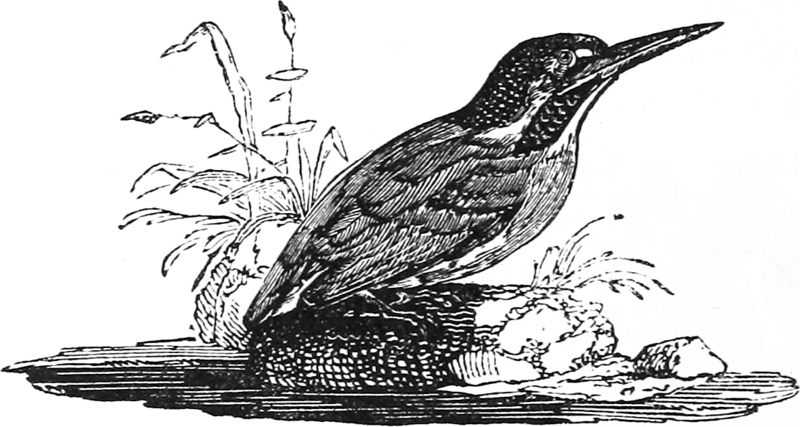
\includegraphics[scale=0.35]{images/Alycon.png}
        \end{figure}
        \vspace{0.5cm}
        \Huge
        \textbf{\textsc{Matematyka Dyskretna}}
        
        \vspace{0.5cm}
        \Large
        \textsc{Wybrane Dowody}
        
        \normalsize
        
        
        \line(1,0){330}
        
        \vspace{1cm}
        \textit{,,Myślę, że 7 punktów na 20 to nie jest zły wynik''}
        \vspace{1cm}

        \textit{\textsc{Popełnione przez}}\\
        \vspace{5mm}

        \textbf{\textsc{Dziurawy Ponton \\ Załatany Ponton \\ Puchaty Pompon \\ Zatopiony Ponton \\ Tonący Ponton \\ Notnop}}

        \vfill

        Kraków \\
        Anno Domini 2023
        
    \end{center}
    
\end{titlepage}


\tableofcontents
\section*{Licencja}
    \begin{figure}[h]
    	\begin{minipage}[c]{0.25\textwidth}
    		
\includegraphics[width=0.7\textwidth]{images/licencja.png}
    	\end{minipage}\hfill
    	\begin{minipage}[c]{0.75\textwidth}
    		\caption*{
    			Ten utwór jest dostępny na 
    			\href{https://creativecommons.org/licenses/by-sa/4.0/}{licencji Creative Commons Uznanie autorstwa
    			na tych samych warunkach 4.0 Międzynarodowe.}
    		}
    	\end{minipage}
    \end{figure}

% Actual content
\mainmatter

\chapter{Kombinatoryka}
 % Żeby nie było syfu to kolejne sekcje dodajemy do chapters/
% A potem includujemy za pomocą \input{chapters/...}

% Używamy \( \) i \[ \] zamiast dolarów -- tak jak się robi w LaTeXu


\documentclass[12pt, a4paper, polish, openany]{book}

% Please, let's familiarize ourselves with notatki.sty and tcs.sty so that we don't reinvent the wheel
\usepackage{notatki}

\fancyhead[L]{\textbf{\textit{MD}}}
\author{
}
\title{TCS and shitposting}


\begin{document}

% Front page and table of contents
\frontmatter

\begin{titlepage} 

    \begin{center}
         \begin{figure}[h]
            \centering
            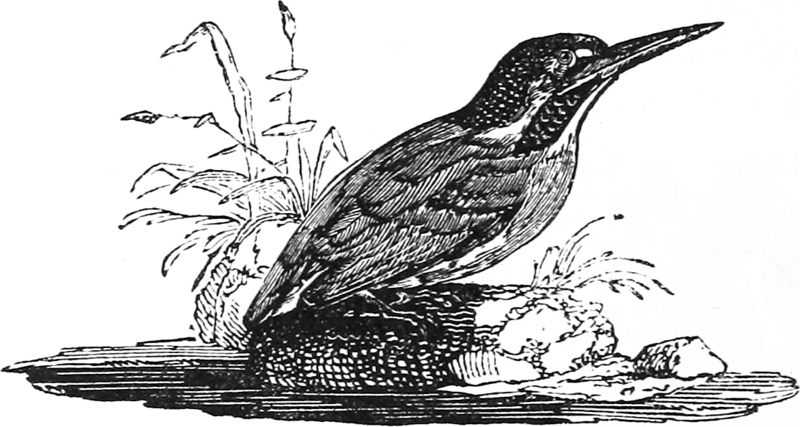
\includegraphics[scale=0.35]{images/Alycon.png}
        \end{figure}
        \vspace{0.5cm}
        \Huge
        \textbf{\textsc{Matematyka Dyskretna}}
        
        \vspace{0.5cm}
        \Large
        \textsc{Wybrane Dowody}
        
        \normalsize
        
        
        \line(1,0){330}
        
        \vspace{1cm}
        \textit{,,Myślę, że 7 punktów na 20 to nie jest zły wynik''}
        \vspace{1cm}

        \textit{\textsc{Popełnione przez}}\\
        \vspace{5mm}

        \textbf{\textsc{Dziurawy Ponton \\ Załatany Ponton \\ Puchaty Pompon \\ Zatopiony Ponton \\ Tonący Ponton \\ Notnop}}

        \vfill

        Kraków \\
        Anno Domini 2023
        
    \end{center}
    
\end{titlepage}


\tableofcontents
\section*{Licencja}
    \begin{figure}[h]
    	\begin{minipage}[c]{0.25\textwidth}
    		
\includegraphics[width=0.7\textwidth]{images/licencja.png}
    	\end{minipage}\hfill
    	\begin{minipage}[c]{0.75\textwidth}
    		\caption*{
    			Ten utwór jest dostępny na 
    			\href{https://creativecommons.org/licenses/by-sa/4.0/}{licencji Creative Commons Uznanie autorstwa
    			na tych samych warunkach 4.0 Międzynarodowe.}
    		}
    	\end{minipage}
    \end{figure}

% Actual content
\mainmatter

\chapter{Kombinatoryka}
 % Żeby nie było syfu to kolejne sekcje dodajemy do chapters/
% A potem includujemy za pomocą \input{chapters/...}

% Używamy \( \) i \[ \] zamiast dolarów -- tak jak się robi w LaTeXu


\documentclass[12pt, a4paper, polish, openany]{book}

% Please, let's familiarize ourselves with notatki.sty and tcs.sty so that we don't reinvent the wheel
\usepackage{notatki}

\fancyhead[L]{\textbf{\textit{MD}}}
\author{
}
\title{TCS and shitposting}


\begin{document}

% Front page and table of contents
\frontmatter

\input{titlepage}

\tableofcontents
\input{license}

% Actual content
\mainmatter

\chapter{Kombinatoryka}
\input{chapters/combinatorics/main}

\chapter{Zasada włączeń i wyłączeń}
\input{chapters/exclusion-inclusion/main}

\chapter{Posety}
\input{chapters/posets/main}

\chapter{Twierdzenie Ramseya}
\input{chapters/ramsey/main}

\chapter{Funkcje tworzące}
\input{chapters/generating_functions/main}

\chapter{Przepływy}
\input{chapters/flows/main}

\chapter{Skojarzenia}
\input{chapters/matchings/main}

\chapter{Kolorowanie grafów}
\input{chapters/graph-coloring/main}

\chapter{Grafy, ale nie kolorowanie}
\input{chapters/graph-misc/main}

\end{document}

\chapter{Zasada włączeń i wyłączeń}
 % Żeby nie było syfu to kolejne sekcje dodajemy do chapters/
% A potem includujemy za pomocą \input{chapters/...}

% Używamy \( \) i \[ \] zamiast dolarów -- tak jak się robi w LaTeXu


\documentclass[12pt, a4paper, polish, openany]{book}

% Please, let's familiarize ourselves with notatki.sty and tcs.sty so that we don't reinvent the wheel
\usepackage{notatki}

\fancyhead[L]{\textbf{\textit{MD}}}
\author{
}
\title{TCS and shitposting}


\begin{document}

% Front page and table of contents
\frontmatter

\input{titlepage}

\tableofcontents
\input{license}

% Actual content
\mainmatter

\chapter{Kombinatoryka}
\input{chapters/combinatorics/main}

\chapter{Zasada włączeń i wyłączeń}
\input{chapters/exclusion-inclusion/main}

\chapter{Posety}
\input{chapters/posets/main}

\chapter{Twierdzenie Ramseya}
\input{chapters/ramsey/main}

\chapter{Funkcje tworzące}
\input{chapters/generating_functions/main}

\chapter{Przepływy}
\input{chapters/flows/main}

\chapter{Skojarzenia}
\input{chapters/matchings/main}

\chapter{Kolorowanie grafów}
\input{chapters/graph-coloring/main}

\chapter{Grafy, ale nie kolorowanie}
\input{chapters/graph-misc/main}

\end{document}

\chapter{Posety}
 % Żeby nie było syfu to kolejne sekcje dodajemy do chapters/
% A potem includujemy za pomocą \input{chapters/...}

% Używamy \( \) i \[ \] zamiast dolarów -- tak jak się robi w LaTeXu


\documentclass[12pt, a4paper, polish, openany]{book}

% Please, let's familiarize ourselves with notatki.sty and tcs.sty so that we don't reinvent the wheel
\usepackage{notatki}

\fancyhead[L]{\textbf{\textit{MD}}}
\author{
}
\title{TCS and shitposting}


\begin{document}

% Front page and table of contents
\frontmatter

\input{titlepage}

\tableofcontents
\input{license}

% Actual content
\mainmatter

\chapter{Kombinatoryka}
\input{chapters/combinatorics/main}

\chapter{Zasada włączeń i wyłączeń}
\input{chapters/exclusion-inclusion/main}

\chapter{Posety}
\input{chapters/posets/main}

\chapter{Twierdzenie Ramseya}
\input{chapters/ramsey/main}

\chapter{Funkcje tworzące}
\input{chapters/generating_functions/main}

\chapter{Przepływy}
\input{chapters/flows/main}

\chapter{Skojarzenia}
\input{chapters/matchings/main}

\chapter{Kolorowanie grafów}
\input{chapters/graph-coloring/main}

\chapter{Grafy, ale nie kolorowanie}
\input{chapters/graph-misc/main}

\end{document}

\chapter{Twierdzenie Ramseya}
 % Żeby nie było syfu to kolejne sekcje dodajemy do chapters/
% A potem includujemy za pomocą \input{chapters/...}

% Używamy \( \) i \[ \] zamiast dolarów -- tak jak się robi w LaTeXu


\documentclass[12pt, a4paper, polish, openany]{book}

% Please, let's familiarize ourselves with notatki.sty and tcs.sty so that we don't reinvent the wheel
\usepackage{notatki}

\fancyhead[L]{\textbf{\textit{MD}}}
\author{
}
\title{TCS and shitposting}


\begin{document}

% Front page and table of contents
\frontmatter

\input{titlepage}

\tableofcontents
\input{license}

% Actual content
\mainmatter

\chapter{Kombinatoryka}
\input{chapters/combinatorics/main}

\chapter{Zasada włączeń i wyłączeń}
\input{chapters/exclusion-inclusion/main}

\chapter{Posety}
\input{chapters/posets/main}

\chapter{Twierdzenie Ramseya}
\input{chapters/ramsey/main}

\chapter{Funkcje tworzące}
\input{chapters/generating_functions/main}

\chapter{Przepływy}
\input{chapters/flows/main}

\chapter{Skojarzenia}
\input{chapters/matchings/main}

\chapter{Kolorowanie grafów}
\input{chapters/graph-coloring/main}

\chapter{Grafy, ale nie kolorowanie}
\input{chapters/graph-misc/main}

\end{document}

\chapter{Funkcje tworzące}
 % Żeby nie było syfu to kolejne sekcje dodajemy do chapters/
% A potem includujemy za pomocą \input{chapters/...}

% Używamy \( \) i \[ \] zamiast dolarów -- tak jak się robi w LaTeXu


\documentclass[12pt, a4paper, polish, openany]{book}

% Please, let's familiarize ourselves with notatki.sty and tcs.sty so that we don't reinvent the wheel
\usepackage{notatki}

\fancyhead[L]{\textbf{\textit{MD}}}
\author{
}
\title{TCS and shitposting}


\begin{document}

% Front page and table of contents
\frontmatter

\input{titlepage}

\tableofcontents
\input{license}

% Actual content
\mainmatter

\chapter{Kombinatoryka}
\input{chapters/combinatorics/main}

\chapter{Zasada włączeń i wyłączeń}
\input{chapters/exclusion-inclusion/main}

\chapter{Posety}
\input{chapters/posets/main}

\chapter{Twierdzenie Ramseya}
\input{chapters/ramsey/main}

\chapter{Funkcje tworzące}
\input{chapters/generating_functions/main}

\chapter{Przepływy}
\input{chapters/flows/main}

\chapter{Skojarzenia}
\input{chapters/matchings/main}

\chapter{Kolorowanie grafów}
\input{chapters/graph-coloring/main}

\chapter{Grafy, ale nie kolorowanie}
\input{chapters/graph-misc/main}

\end{document}

\chapter{Przepływy}
 % Żeby nie było syfu to kolejne sekcje dodajemy do chapters/
% A potem includujemy za pomocą \input{chapters/...}

% Używamy \( \) i \[ \] zamiast dolarów -- tak jak się robi w LaTeXu


\documentclass[12pt, a4paper, polish, openany]{book}

% Please, let's familiarize ourselves with notatki.sty and tcs.sty so that we don't reinvent the wheel
\usepackage{notatki}

\fancyhead[L]{\textbf{\textit{MD}}}
\author{
}
\title{TCS and shitposting}


\begin{document}

% Front page and table of contents
\frontmatter

\input{titlepage}

\tableofcontents
\input{license}

% Actual content
\mainmatter

\chapter{Kombinatoryka}
\input{chapters/combinatorics/main}

\chapter{Zasada włączeń i wyłączeń}
\input{chapters/exclusion-inclusion/main}

\chapter{Posety}
\input{chapters/posets/main}

\chapter{Twierdzenie Ramseya}
\input{chapters/ramsey/main}

\chapter{Funkcje tworzące}
\input{chapters/generating_functions/main}

\chapter{Przepływy}
\input{chapters/flows/main}

\chapter{Skojarzenia}
\input{chapters/matchings/main}

\chapter{Kolorowanie grafów}
\input{chapters/graph-coloring/main}

\chapter{Grafy, ale nie kolorowanie}
\input{chapters/graph-misc/main}

\end{document}

\chapter{Skojarzenia}
 % Żeby nie było syfu to kolejne sekcje dodajemy do chapters/
% A potem includujemy za pomocą \input{chapters/...}

% Używamy \( \) i \[ \] zamiast dolarów -- tak jak się robi w LaTeXu


\documentclass[12pt, a4paper, polish, openany]{book}

% Please, let's familiarize ourselves with notatki.sty and tcs.sty so that we don't reinvent the wheel
\usepackage{notatki}

\fancyhead[L]{\textbf{\textit{MD}}}
\author{
}
\title{TCS and shitposting}


\begin{document}

% Front page and table of contents
\frontmatter

\input{titlepage}

\tableofcontents
\input{license}

% Actual content
\mainmatter

\chapter{Kombinatoryka}
\input{chapters/combinatorics/main}

\chapter{Zasada włączeń i wyłączeń}
\input{chapters/exclusion-inclusion/main}

\chapter{Posety}
\input{chapters/posets/main}

\chapter{Twierdzenie Ramseya}
\input{chapters/ramsey/main}

\chapter{Funkcje tworzące}
\input{chapters/generating_functions/main}

\chapter{Przepływy}
\input{chapters/flows/main}

\chapter{Skojarzenia}
\input{chapters/matchings/main}

\chapter{Kolorowanie grafów}
\input{chapters/graph-coloring/main}

\chapter{Grafy, ale nie kolorowanie}
\input{chapters/graph-misc/main}

\end{document}

\chapter{Kolorowanie grafów}
 % Żeby nie było syfu to kolejne sekcje dodajemy do chapters/
% A potem includujemy za pomocą \input{chapters/...}

% Używamy \( \) i \[ \] zamiast dolarów -- tak jak się robi w LaTeXu


\documentclass[12pt, a4paper, polish, openany]{book}

% Please, let's familiarize ourselves with notatki.sty and tcs.sty so that we don't reinvent the wheel
\usepackage{notatki}

\fancyhead[L]{\textbf{\textit{MD}}}
\author{
}
\title{TCS and shitposting}


\begin{document}

% Front page and table of contents
\frontmatter

\input{titlepage}

\tableofcontents
\input{license}

% Actual content
\mainmatter

\chapter{Kombinatoryka}
\input{chapters/combinatorics/main}

\chapter{Zasada włączeń i wyłączeń}
\input{chapters/exclusion-inclusion/main}

\chapter{Posety}
\input{chapters/posets/main}

\chapter{Twierdzenie Ramseya}
\input{chapters/ramsey/main}

\chapter{Funkcje tworzące}
\input{chapters/generating_functions/main}

\chapter{Przepływy}
\input{chapters/flows/main}

\chapter{Skojarzenia}
\input{chapters/matchings/main}

\chapter{Kolorowanie grafów}
\input{chapters/graph-coloring/main}

\chapter{Grafy, ale nie kolorowanie}
\input{chapters/graph-misc/main}

\end{document}

\chapter{Grafy, ale nie kolorowanie}
 % Żeby nie było syfu to kolejne sekcje dodajemy do chapters/
% A potem includujemy za pomocą \input{chapters/...}

% Używamy \( \) i \[ \] zamiast dolarów -- tak jak się robi w LaTeXu


\documentclass[12pt, a4paper, polish, openany]{book}

% Please, let's familiarize ourselves with notatki.sty and tcs.sty so that we don't reinvent the wheel
\usepackage{notatki}

\fancyhead[L]{\textbf{\textit{MD}}}
\author{
}
\title{TCS and shitposting}


\begin{document}

% Front page and table of contents
\frontmatter

\input{titlepage}

\tableofcontents
\input{license}

% Actual content
\mainmatter

\chapter{Kombinatoryka}
\input{chapters/combinatorics/main}

\chapter{Zasada włączeń i wyłączeń}
\input{chapters/exclusion-inclusion/main}

\chapter{Posety}
\input{chapters/posets/main}

\chapter{Twierdzenie Ramseya}
\input{chapters/ramsey/main}

\chapter{Funkcje tworzące}
\input{chapters/generating_functions/main}

\chapter{Przepływy}
\input{chapters/flows/main}

\chapter{Skojarzenia}
\input{chapters/matchings/main}

\chapter{Kolorowanie grafów}
\input{chapters/graph-coloring/main}

\chapter{Grafy, ale nie kolorowanie}
\input{chapters/graph-misc/main}

\end{document}

\end{document}

\chapter{Zasada włączeń i wyłączeń}
 % Żeby nie było syfu to kolejne sekcje dodajemy do chapters/
% A potem includujemy za pomocą \input{chapters/...}

% Używamy \( \) i \[ \] zamiast dolarów -- tak jak się robi w LaTeXu


\documentclass[12pt, a4paper, polish, openany]{book}

% Please, let's familiarize ourselves with notatki.sty and tcs.sty so that we don't reinvent the wheel
\usepackage{notatki}

\fancyhead[L]{\textbf{\textit{MD}}}
\author{
}
\title{TCS and shitposting}


\begin{document}

% Front page and table of contents
\frontmatter

\begin{titlepage} 

    \begin{center}
         \begin{figure}[h]
            \centering
            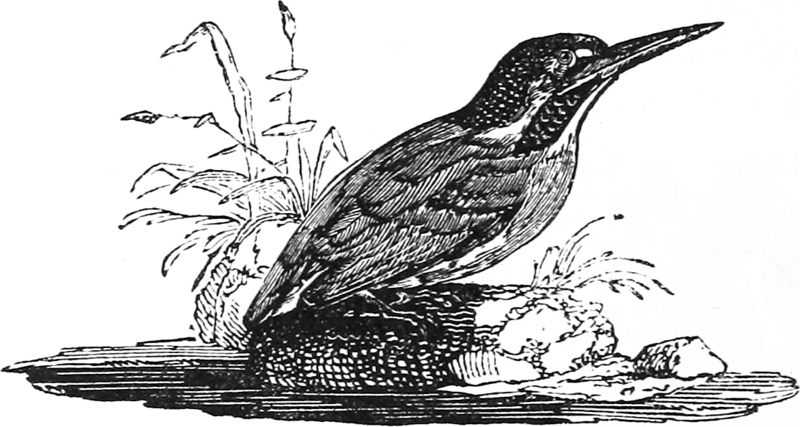
\includegraphics[scale=0.35]{images/Alycon.png}
        \end{figure}
        \vspace{0.5cm}
        \Huge
        \textbf{\textsc{Matematyka Dyskretna}}
        
        \vspace{0.5cm}
        \Large
        \textsc{Wybrane Dowody}
        
        \normalsize
        
        
        \line(1,0){330}
        
        \vspace{1cm}
        \textit{,,Myślę, że 7 punktów na 20 to nie jest zły wynik''}
        \vspace{1cm}

        \textit{\textsc{Popełnione przez}}\\
        \vspace{5mm}

        \textbf{\textsc{Dziurawy Ponton \\ Załatany Ponton \\ Puchaty Pompon \\ Zatopiony Ponton \\ Tonący Ponton \\ Notnop}}

        \vfill

        Kraków \\
        Anno Domini 2023
        
    \end{center}
    
\end{titlepage}


\tableofcontents
\section*{Licencja}
    \begin{figure}[h]
    	\begin{minipage}[c]{0.25\textwidth}
    		
\includegraphics[width=0.7\textwidth]{images/licencja.png}
    	\end{minipage}\hfill
    	\begin{minipage}[c]{0.75\textwidth}
    		\caption*{
    			Ten utwór jest dostępny na 
    			\href{https://creativecommons.org/licenses/by-sa/4.0/}{licencji Creative Commons Uznanie autorstwa
    			na tych samych warunkach 4.0 Międzynarodowe.}
    		}
    	\end{minipage}
    \end{figure}

% Actual content
\mainmatter

\chapter{Kombinatoryka}
 % Żeby nie było syfu to kolejne sekcje dodajemy do chapters/
% A potem includujemy za pomocą \input{chapters/...}

% Używamy \( \) i \[ \] zamiast dolarów -- tak jak się robi w LaTeXu


\documentclass[12pt, a4paper, polish, openany]{book}

% Please, let's familiarize ourselves with notatki.sty and tcs.sty so that we don't reinvent the wheel
\usepackage{notatki}

\fancyhead[L]{\textbf{\textit{MD}}}
\author{
}
\title{TCS and shitposting}


\begin{document}

% Front page and table of contents
\frontmatter

\input{titlepage}

\tableofcontents
\input{license}

% Actual content
\mainmatter

\chapter{Kombinatoryka}
\input{chapters/combinatorics/main}

\chapter{Zasada włączeń i wyłączeń}
\input{chapters/exclusion-inclusion/main}

\chapter{Posety}
\input{chapters/posets/main}

\chapter{Twierdzenie Ramseya}
\input{chapters/ramsey/main}

\chapter{Funkcje tworzące}
\input{chapters/generating_functions/main}

\chapter{Przepływy}
\input{chapters/flows/main}

\chapter{Skojarzenia}
\input{chapters/matchings/main}

\chapter{Kolorowanie grafów}
\input{chapters/graph-coloring/main}

\chapter{Grafy, ale nie kolorowanie}
\input{chapters/graph-misc/main}

\end{document}

\chapter{Zasada włączeń i wyłączeń}
 % Żeby nie było syfu to kolejne sekcje dodajemy do chapters/
% A potem includujemy za pomocą \input{chapters/...}

% Używamy \( \) i \[ \] zamiast dolarów -- tak jak się robi w LaTeXu


\documentclass[12pt, a4paper, polish, openany]{book}

% Please, let's familiarize ourselves with notatki.sty and tcs.sty so that we don't reinvent the wheel
\usepackage{notatki}

\fancyhead[L]{\textbf{\textit{MD}}}
\author{
}
\title{TCS and shitposting}


\begin{document}

% Front page and table of contents
\frontmatter

\input{titlepage}

\tableofcontents
\input{license}

% Actual content
\mainmatter

\chapter{Kombinatoryka}
\input{chapters/combinatorics/main}

\chapter{Zasada włączeń i wyłączeń}
\input{chapters/exclusion-inclusion/main}

\chapter{Posety}
\input{chapters/posets/main}

\chapter{Twierdzenie Ramseya}
\input{chapters/ramsey/main}

\chapter{Funkcje tworzące}
\input{chapters/generating_functions/main}

\chapter{Przepływy}
\input{chapters/flows/main}

\chapter{Skojarzenia}
\input{chapters/matchings/main}

\chapter{Kolorowanie grafów}
\input{chapters/graph-coloring/main}

\chapter{Grafy, ale nie kolorowanie}
\input{chapters/graph-misc/main}

\end{document}

\chapter{Posety}
 % Żeby nie było syfu to kolejne sekcje dodajemy do chapters/
% A potem includujemy za pomocą \input{chapters/...}

% Używamy \( \) i \[ \] zamiast dolarów -- tak jak się robi w LaTeXu


\documentclass[12pt, a4paper, polish, openany]{book}

% Please, let's familiarize ourselves with notatki.sty and tcs.sty so that we don't reinvent the wheel
\usepackage{notatki}

\fancyhead[L]{\textbf{\textit{MD}}}
\author{
}
\title{TCS and shitposting}


\begin{document}

% Front page and table of contents
\frontmatter

\input{titlepage}

\tableofcontents
\input{license}

% Actual content
\mainmatter

\chapter{Kombinatoryka}
\input{chapters/combinatorics/main}

\chapter{Zasada włączeń i wyłączeń}
\input{chapters/exclusion-inclusion/main}

\chapter{Posety}
\input{chapters/posets/main}

\chapter{Twierdzenie Ramseya}
\input{chapters/ramsey/main}

\chapter{Funkcje tworzące}
\input{chapters/generating_functions/main}

\chapter{Przepływy}
\input{chapters/flows/main}

\chapter{Skojarzenia}
\input{chapters/matchings/main}

\chapter{Kolorowanie grafów}
\input{chapters/graph-coloring/main}

\chapter{Grafy, ale nie kolorowanie}
\input{chapters/graph-misc/main}

\end{document}

\chapter{Twierdzenie Ramseya}
 % Żeby nie było syfu to kolejne sekcje dodajemy do chapters/
% A potem includujemy za pomocą \input{chapters/...}

% Używamy \( \) i \[ \] zamiast dolarów -- tak jak się robi w LaTeXu


\documentclass[12pt, a4paper, polish, openany]{book}

% Please, let's familiarize ourselves with notatki.sty and tcs.sty so that we don't reinvent the wheel
\usepackage{notatki}

\fancyhead[L]{\textbf{\textit{MD}}}
\author{
}
\title{TCS and shitposting}


\begin{document}

% Front page and table of contents
\frontmatter

\input{titlepage}

\tableofcontents
\input{license}

% Actual content
\mainmatter

\chapter{Kombinatoryka}
\input{chapters/combinatorics/main}

\chapter{Zasada włączeń i wyłączeń}
\input{chapters/exclusion-inclusion/main}

\chapter{Posety}
\input{chapters/posets/main}

\chapter{Twierdzenie Ramseya}
\input{chapters/ramsey/main}

\chapter{Funkcje tworzące}
\input{chapters/generating_functions/main}

\chapter{Przepływy}
\input{chapters/flows/main}

\chapter{Skojarzenia}
\input{chapters/matchings/main}

\chapter{Kolorowanie grafów}
\input{chapters/graph-coloring/main}

\chapter{Grafy, ale nie kolorowanie}
\input{chapters/graph-misc/main}

\end{document}

\chapter{Funkcje tworzące}
 % Żeby nie było syfu to kolejne sekcje dodajemy do chapters/
% A potem includujemy za pomocą \input{chapters/...}

% Używamy \( \) i \[ \] zamiast dolarów -- tak jak się robi w LaTeXu


\documentclass[12pt, a4paper, polish, openany]{book}

% Please, let's familiarize ourselves with notatki.sty and tcs.sty so that we don't reinvent the wheel
\usepackage{notatki}

\fancyhead[L]{\textbf{\textit{MD}}}
\author{
}
\title{TCS and shitposting}


\begin{document}

% Front page and table of contents
\frontmatter

\input{titlepage}

\tableofcontents
\input{license}

% Actual content
\mainmatter

\chapter{Kombinatoryka}
\input{chapters/combinatorics/main}

\chapter{Zasada włączeń i wyłączeń}
\input{chapters/exclusion-inclusion/main}

\chapter{Posety}
\input{chapters/posets/main}

\chapter{Twierdzenie Ramseya}
\input{chapters/ramsey/main}

\chapter{Funkcje tworzące}
\input{chapters/generating_functions/main}

\chapter{Przepływy}
\input{chapters/flows/main}

\chapter{Skojarzenia}
\input{chapters/matchings/main}

\chapter{Kolorowanie grafów}
\input{chapters/graph-coloring/main}

\chapter{Grafy, ale nie kolorowanie}
\input{chapters/graph-misc/main}

\end{document}

\chapter{Przepływy}
 % Żeby nie było syfu to kolejne sekcje dodajemy do chapters/
% A potem includujemy za pomocą \input{chapters/...}

% Używamy \( \) i \[ \] zamiast dolarów -- tak jak się robi w LaTeXu


\documentclass[12pt, a4paper, polish, openany]{book}

% Please, let's familiarize ourselves with notatki.sty and tcs.sty so that we don't reinvent the wheel
\usepackage{notatki}

\fancyhead[L]{\textbf{\textit{MD}}}
\author{
}
\title{TCS and shitposting}


\begin{document}

% Front page and table of contents
\frontmatter

\input{titlepage}

\tableofcontents
\input{license}

% Actual content
\mainmatter

\chapter{Kombinatoryka}
\input{chapters/combinatorics/main}

\chapter{Zasada włączeń i wyłączeń}
\input{chapters/exclusion-inclusion/main}

\chapter{Posety}
\input{chapters/posets/main}

\chapter{Twierdzenie Ramseya}
\input{chapters/ramsey/main}

\chapter{Funkcje tworzące}
\input{chapters/generating_functions/main}

\chapter{Przepływy}
\input{chapters/flows/main}

\chapter{Skojarzenia}
\input{chapters/matchings/main}

\chapter{Kolorowanie grafów}
\input{chapters/graph-coloring/main}

\chapter{Grafy, ale nie kolorowanie}
\input{chapters/graph-misc/main}

\end{document}

\chapter{Skojarzenia}
 % Żeby nie było syfu to kolejne sekcje dodajemy do chapters/
% A potem includujemy za pomocą \input{chapters/...}

% Używamy \( \) i \[ \] zamiast dolarów -- tak jak się robi w LaTeXu


\documentclass[12pt, a4paper, polish, openany]{book}

% Please, let's familiarize ourselves with notatki.sty and tcs.sty so that we don't reinvent the wheel
\usepackage{notatki}

\fancyhead[L]{\textbf{\textit{MD}}}
\author{
}
\title{TCS and shitposting}


\begin{document}

% Front page and table of contents
\frontmatter

\input{titlepage}

\tableofcontents
\input{license}

% Actual content
\mainmatter

\chapter{Kombinatoryka}
\input{chapters/combinatorics/main}

\chapter{Zasada włączeń i wyłączeń}
\input{chapters/exclusion-inclusion/main}

\chapter{Posety}
\input{chapters/posets/main}

\chapter{Twierdzenie Ramseya}
\input{chapters/ramsey/main}

\chapter{Funkcje tworzące}
\input{chapters/generating_functions/main}

\chapter{Przepływy}
\input{chapters/flows/main}

\chapter{Skojarzenia}
\input{chapters/matchings/main}

\chapter{Kolorowanie grafów}
\input{chapters/graph-coloring/main}

\chapter{Grafy, ale nie kolorowanie}
\input{chapters/graph-misc/main}

\end{document}

\chapter{Kolorowanie grafów}
 % Żeby nie było syfu to kolejne sekcje dodajemy do chapters/
% A potem includujemy za pomocą \input{chapters/...}

% Używamy \( \) i \[ \] zamiast dolarów -- tak jak się robi w LaTeXu


\documentclass[12pt, a4paper, polish, openany]{book}

% Please, let's familiarize ourselves with notatki.sty and tcs.sty so that we don't reinvent the wheel
\usepackage{notatki}

\fancyhead[L]{\textbf{\textit{MD}}}
\author{
}
\title{TCS and shitposting}


\begin{document}

% Front page and table of contents
\frontmatter

\input{titlepage}

\tableofcontents
\input{license}

% Actual content
\mainmatter

\chapter{Kombinatoryka}
\input{chapters/combinatorics/main}

\chapter{Zasada włączeń i wyłączeń}
\input{chapters/exclusion-inclusion/main}

\chapter{Posety}
\input{chapters/posets/main}

\chapter{Twierdzenie Ramseya}
\input{chapters/ramsey/main}

\chapter{Funkcje tworzące}
\input{chapters/generating_functions/main}

\chapter{Przepływy}
\input{chapters/flows/main}

\chapter{Skojarzenia}
\input{chapters/matchings/main}

\chapter{Kolorowanie grafów}
\input{chapters/graph-coloring/main}

\chapter{Grafy, ale nie kolorowanie}
\input{chapters/graph-misc/main}

\end{document}

\chapter{Grafy, ale nie kolorowanie}
 % Żeby nie było syfu to kolejne sekcje dodajemy do chapters/
% A potem includujemy za pomocą \input{chapters/...}

% Używamy \( \) i \[ \] zamiast dolarów -- tak jak się robi w LaTeXu


\documentclass[12pt, a4paper, polish, openany]{book}

% Please, let's familiarize ourselves with notatki.sty and tcs.sty so that we don't reinvent the wheel
\usepackage{notatki}

\fancyhead[L]{\textbf{\textit{MD}}}
\author{
}
\title{TCS and shitposting}


\begin{document}

% Front page and table of contents
\frontmatter

\input{titlepage}

\tableofcontents
\input{license}

% Actual content
\mainmatter

\chapter{Kombinatoryka}
\input{chapters/combinatorics/main}

\chapter{Zasada włączeń i wyłączeń}
\input{chapters/exclusion-inclusion/main}

\chapter{Posety}
\input{chapters/posets/main}

\chapter{Twierdzenie Ramseya}
\input{chapters/ramsey/main}

\chapter{Funkcje tworzące}
\input{chapters/generating_functions/main}

\chapter{Przepływy}
\input{chapters/flows/main}

\chapter{Skojarzenia}
\input{chapters/matchings/main}

\chapter{Kolorowanie grafów}
\input{chapters/graph-coloring/main}

\chapter{Grafy, ale nie kolorowanie}
\input{chapters/graph-misc/main}

\end{document}

\end{document}

\chapter{Posety}
 % Żeby nie było syfu to kolejne sekcje dodajemy do chapters/
% A potem includujemy za pomocą \input{chapters/...}

% Używamy \( \) i \[ \] zamiast dolarów -- tak jak się robi w LaTeXu


\documentclass[12pt, a4paper, polish, openany]{book}

% Please, let's familiarize ourselves with notatki.sty and tcs.sty so that we don't reinvent the wheel
\usepackage{notatki}

\fancyhead[L]{\textbf{\textit{MD}}}
\author{
}
\title{TCS and shitposting}


\begin{document}

% Front page and table of contents
\frontmatter

\begin{titlepage} 

    \begin{center}
         \begin{figure}[h]
            \centering
            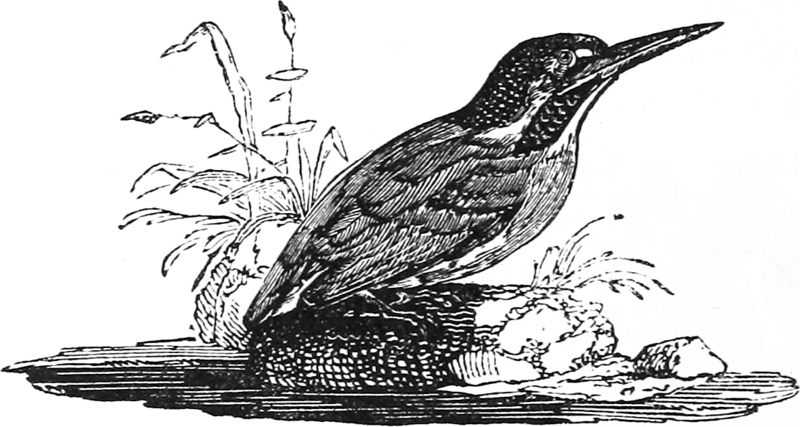
\includegraphics[scale=0.35]{images/Alycon.png}
        \end{figure}
        \vspace{0.5cm}
        \Huge
        \textbf{\textsc{Matematyka Dyskretna}}
        
        \vspace{0.5cm}
        \Large
        \textsc{Wybrane Dowody}
        
        \normalsize
        
        
        \line(1,0){330}
        
        \vspace{1cm}
        \textit{,,Myślę, że 7 punktów na 20 to nie jest zły wynik''}
        \vspace{1cm}

        \textit{\textsc{Popełnione przez}}\\
        \vspace{5mm}

        \textbf{\textsc{Dziurawy Ponton \\ Załatany Ponton \\ Puchaty Pompon \\ Zatopiony Ponton \\ Tonący Ponton \\ Notnop}}

        \vfill

        Kraków \\
        Anno Domini 2023
        
    \end{center}
    
\end{titlepage}


\tableofcontents
\section*{Licencja}
    \begin{figure}[h]
    	\begin{minipage}[c]{0.25\textwidth}
    		
\includegraphics[width=0.7\textwidth]{images/licencja.png}
    	\end{minipage}\hfill
    	\begin{minipage}[c]{0.75\textwidth}
    		\caption*{
    			Ten utwór jest dostępny na 
    			\href{https://creativecommons.org/licenses/by-sa/4.0/}{licencji Creative Commons Uznanie autorstwa
    			na tych samych warunkach 4.0 Międzynarodowe.}
    		}
    	\end{minipage}
    \end{figure}

% Actual content
\mainmatter

\chapter{Kombinatoryka}
 % Żeby nie było syfu to kolejne sekcje dodajemy do chapters/
% A potem includujemy za pomocą \input{chapters/...}

% Używamy \( \) i \[ \] zamiast dolarów -- tak jak się robi w LaTeXu


\documentclass[12pt, a4paper, polish, openany]{book}

% Please, let's familiarize ourselves with notatki.sty and tcs.sty so that we don't reinvent the wheel
\usepackage{notatki}

\fancyhead[L]{\textbf{\textit{MD}}}
\author{
}
\title{TCS and shitposting}


\begin{document}

% Front page and table of contents
\frontmatter

\input{titlepage}

\tableofcontents
\input{license}

% Actual content
\mainmatter

\chapter{Kombinatoryka}
\input{chapters/combinatorics/main}

\chapter{Zasada włączeń i wyłączeń}
\input{chapters/exclusion-inclusion/main}

\chapter{Posety}
\input{chapters/posets/main}

\chapter{Twierdzenie Ramseya}
\input{chapters/ramsey/main}

\chapter{Funkcje tworzące}
\input{chapters/generating_functions/main}

\chapter{Przepływy}
\input{chapters/flows/main}

\chapter{Skojarzenia}
\input{chapters/matchings/main}

\chapter{Kolorowanie grafów}
\input{chapters/graph-coloring/main}

\chapter{Grafy, ale nie kolorowanie}
\input{chapters/graph-misc/main}

\end{document}

\chapter{Zasada włączeń i wyłączeń}
 % Żeby nie było syfu to kolejne sekcje dodajemy do chapters/
% A potem includujemy za pomocą \input{chapters/...}

% Używamy \( \) i \[ \] zamiast dolarów -- tak jak się robi w LaTeXu


\documentclass[12pt, a4paper, polish, openany]{book}

% Please, let's familiarize ourselves with notatki.sty and tcs.sty so that we don't reinvent the wheel
\usepackage{notatki}

\fancyhead[L]{\textbf{\textit{MD}}}
\author{
}
\title{TCS and shitposting}


\begin{document}

% Front page and table of contents
\frontmatter

\input{titlepage}

\tableofcontents
\input{license}

% Actual content
\mainmatter

\chapter{Kombinatoryka}
\input{chapters/combinatorics/main}

\chapter{Zasada włączeń i wyłączeń}
\input{chapters/exclusion-inclusion/main}

\chapter{Posety}
\input{chapters/posets/main}

\chapter{Twierdzenie Ramseya}
\input{chapters/ramsey/main}

\chapter{Funkcje tworzące}
\input{chapters/generating_functions/main}

\chapter{Przepływy}
\input{chapters/flows/main}

\chapter{Skojarzenia}
\input{chapters/matchings/main}

\chapter{Kolorowanie grafów}
\input{chapters/graph-coloring/main}

\chapter{Grafy, ale nie kolorowanie}
\input{chapters/graph-misc/main}

\end{document}

\chapter{Posety}
 % Żeby nie było syfu to kolejne sekcje dodajemy do chapters/
% A potem includujemy za pomocą \input{chapters/...}

% Używamy \( \) i \[ \] zamiast dolarów -- tak jak się robi w LaTeXu


\documentclass[12pt, a4paper, polish, openany]{book}

% Please, let's familiarize ourselves with notatki.sty and tcs.sty so that we don't reinvent the wheel
\usepackage{notatki}

\fancyhead[L]{\textbf{\textit{MD}}}
\author{
}
\title{TCS and shitposting}


\begin{document}

% Front page and table of contents
\frontmatter

\input{titlepage}

\tableofcontents
\input{license}

% Actual content
\mainmatter

\chapter{Kombinatoryka}
\input{chapters/combinatorics/main}

\chapter{Zasada włączeń i wyłączeń}
\input{chapters/exclusion-inclusion/main}

\chapter{Posety}
\input{chapters/posets/main}

\chapter{Twierdzenie Ramseya}
\input{chapters/ramsey/main}

\chapter{Funkcje tworzące}
\input{chapters/generating_functions/main}

\chapter{Przepływy}
\input{chapters/flows/main}

\chapter{Skojarzenia}
\input{chapters/matchings/main}

\chapter{Kolorowanie grafów}
\input{chapters/graph-coloring/main}

\chapter{Grafy, ale nie kolorowanie}
\input{chapters/graph-misc/main}

\end{document}

\chapter{Twierdzenie Ramseya}
 % Żeby nie było syfu to kolejne sekcje dodajemy do chapters/
% A potem includujemy za pomocą \input{chapters/...}

% Używamy \( \) i \[ \] zamiast dolarów -- tak jak się robi w LaTeXu


\documentclass[12pt, a4paper, polish, openany]{book}

% Please, let's familiarize ourselves with notatki.sty and tcs.sty so that we don't reinvent the wheel
\usepackage{notatki}

\fancyhead[L]{\textbf{\textit{MD}}}
\author{
}
\title{TCS and shitposting}


\begin{document}

% Front page and table of contents
\frontmatter

\input{titlepage}

\tableofcontents
\input{license}

% Actual content
\mainmatter

\chapter{Kombinatoryka}
\input{chapters/combinatorics/main}

\chapter{Zasada włączeń i wyłączeń}
\input{chapters/exclusion-inclusion/main}

\chapter{Posety}
\input{chapters/posets/main}

\chapter{Twierdzenie Ramseya}
\input{chapters/ramsey/main}

\chapter{Funkcje tworzące}
\input{chapters/generating_functions/main}

\chapter{Przepływy}
\input{chapters/flows/main}

\chapter{Skojarzenia}
\input{chapters/matchings/main}

\chapter{Kolorowanie grafów}
\input{chapters/graph-coloring/main}

\chapter{Grafy, ale nie kolorowanie}
\input{chapters/graph-misc/main}

\end{document}

\chapter{Funkcje tworzące}
 % Żeby nie było syfu to kolejne sekcje dodajemy do chapters/
% A potem includujemy za pomocą \input{chapters/...}

% Używamy \( \) i \[ \] zamiast dolarów -- tak jak się robi w LaTeXu


\documentclass[12pt, a4paper, polish, openany]{book}

% Please, let's familiarize ourselves with notatki.sty and tcs.sty so that we don't reinvent the wheel
\usepackage{notatki}

\fancyhead[L]{\textbf{\textit{MD}}}
\author{
}
\title{TCS and shitposting}


\begin{document}

% Front page and table of contents
\frontmatter

\input{titlepage}

\tableofcontents
\input{license}

% Actual content
\mainmatter

\chapter{Kombinatoryka}
\input{chapters/combinatorics/main}

\chapter{Zasada włączeń i wyłączeń}
\input{chapters/exclusion-inclusion/main}

\chapter{Posety}
\input{chapters/posets/main}

\chapter{Twierdzenie Ramseya}
\input{chapters/ramsey/main}

\chapter{Funkcje tworzące}
\input{chapters/generating_functions/main}

\chapter{Przepływy}
\input{chapters/flows/main}

\chapter{Skojarzenia}
\input{chapters/matchings/main}

\chapter{Kolorowanie grafów}
\input{chapters/graph-coloring/main}

\chapter{Grafy, ale nie kolorowanie}
\input{chapters/graph-misc/main}

\end{document}

\chapter{Przepływy}
 % Żeby nie było syfu to kolejne sekcje dodajemy do chapters/
% A potem includujemy za pomocą \input{chapters/...}

% Używamy \( \) i \[ \] zamiast dolarów -- tak jak się robi w LaTeXu


\documentclass[12pt, a4paper, polish, openany]{book}

% Please, let's familiarize ourselves with notatki.sty and tcs.sty so that we don't reinvent the wheel
\usepackage{notatki}

\fancyhead[L]{\textbf{\textit{MD}}}
\author{
}
\title{TCS and shitposting}


\begin{document}

% Front page and table of contents
\frontmatter

\input{titlepage}

\tableofcontents
\input{license}

% Actual content
\mainmatter

\chapter{Kombinatoryka}
\input{chapters/combinatorics/main}

\chapter{Zasada włączeń i wyłączeń}
\input{chapters/exclusion-inclusion/main}

\chapter{Posety}
\input{chapters/posets/main}

\chapter{Twierdzenie Ramseya}
\input{chapters/ramsey/main}

\chapter{Funkcje tworzące}
\input{chapters/generating_functions/main}

\chapter{Przepływy}
\input{chapters/flows/main}

\chapter{Skojarzenia}
\input{chapters/matchings/main}

\chapter{Kolorowanie grafów}
\input{chapters/graph-coloring/main}

\chapter{Grafy, ale nie kolorowanie}
\input{chapters/graph-misc/main}

\end{document}

\chapter{Skojarzenia}
 % Żeby nie było syfu to kolejne sekcje dodajemy do chapters/
% A potem includujemy za pomocą \input{chapters/...}

% Używamy \( \) i \[ \] zamiast dolarów -- tak jak się robi w LaTeXu


\documentclass[12pt, a4paper, polish, openany]{book}

% Please, let's familiarize ourselves with notatki.sty and tcs.sty so that we don't reinvent the wheel
\usepackage{notatki}

\fancyhead[L]{\textbf{\textit{MD}}}
\author{
}
\title{TCS and shitposting}


\begin{document}

% Front page and table of contents
\frontmatter

\input{titlepage}

\tableofcontents
\input{license}

% Actual content
\mainmatter

\chapter{Kombinatoryka}
\input{chapters/combinatorics/main}

\chapter{Zasada włączeń i wyłączeń}
\input{chapters/exclusion-inclusion/main}

\chapter{Posety}
\input{chapters/posets/main}

\chapter{Twierdzenie Ramseya}
\input{chapters/ramsey/main}

\chapter{Funkcje tworzące}
\input{chapters/generating_functions/main}

\chapter{Przepływy}
\input{chapters/flows/main}

\chapter{Skojarzenia}
\input{chapters/matchings/main}

\chapter{Kolorowanie grafów}
\input{chapters/graph-coloring/main}

\chapter{Grafy, ale nie kolorowanie}
\input{chapters/graph-misc/main}

\end{document}

\chapter{Kolorowanie grafów}
 % Żeby nie było syfu to kolejne sekcje dodajemy do chapters/
% A potem includujemy za pomocą \input{chapters/...}

% Używamy \( \) i \[ \] zamiast dolarów -- tak jak się robi w LaTeXu


\documentclass[12pt, a4paper, polish, openany]{book}

% Please, let's familiarize ourselves with notatki.sty and tcs.sty so that we don't reinvent the wheel
\usepackage{notatki}

\fancyhead[L]{\textbf{\textit{MD}}}
\author{
}
\title{TCS and shitposting}


\begin{document}

% Front page and table of contents
\frontmatter

\input{titlepage}

\tableofcontents
\input{license}

% Actual content
\mainmatter

\chapter{Kombinatoryka}
\input{chapters/combinatorics/main}

\chapter{Zasada włączeń i wyłączeń}
\input{chapters/exclusion-inclusion/main}

\chapter{Posety}
\input{chapters/posets/main}

\chapter{Twierdzenie Ramseya}
\input{chapters/ramsey/main}

\chapter{Funkcje tworzące}
\input{chapters/generating_functions/main}

\chapter{Przepływy}
\input{chapters/flows/main}

\chapter{Skojarzenia}
\input{chapters/matchings/main}

\chapter{Kolorowanie grafów}
\input{chapters/graph-coloring/main}

\chapter{Grafy, ale nie kolorowanie}
\input{chapters/graph-misc/main}

\end{document}

\chapter{Grafy, ale nie kolorowanie}
 % Żeby nie było syfu to kolejne sekcje dodajemy do chapters/
% A potem includujemy za pomocą \input{chapters/...}

% Używamy \( \) i \[ \] zamiast dolarów -- tak jak się robi w LaTeXu


\documentclass[12pt, a4paper, polish, openany]{book}

% Please, let's familiarize ourselves with notatki.sty and tcs.sty so that we don't reinvent the wheel
\usepackage{notatki}

\fancyhead[L]{\textbf{\textit{MD}}}
\author{
}
\title{TCS and shitposting}


\begin{document}

% Front page and table of contents
\frontmatter

\input{titlepage}

\tableofcontents
\input{license}

% Actual content
\mainmatter

\chapter{Kombinatoryka}
\input{chapters/combinatorics/main}

\chapter{Zasada włączeń i wyłączeń}
\input{chapters/exclusion-inclusion/main}

\chapter{Posety}
\input{chapters/posets/main}

\chapter{Twierdzenie Ramseya}
\input{chapters/ramsey/main}

\chapter{Funkcje tworzące}
\input{chapters/generating_functions/main}

\chapter{Przepływy}
\input{chapters/flows/main}

\chapter{Skojarzenia}
\input{chapters/matchings/main}

\chapter{Kolorowanie grafów}
\input{chapters/graph-coloring/main}

\chapter{Grafy, ale nie kolorowanie}
\input{chapters/graph-misc/main}

\end{document}

\end{document}

\chapter{Twierdzenie Ramseya}
 % Żeby nie było syfu to kolejne sekcje dodajemy do chapters/
% A potem includujemy za pomocą \input{chapters/...}

% Używamy \( \) i \[ \] zamiast dolarów -- tak jak się robi w LaTeXu


\documentclass[12pt, a4paper, polish, openany]{book}

% Please, let's familiarize ourselves with notatki.sty and tcs.sty so that we don't reinvent the wheel
\usepackage{notatki}

\fancyhead[L]{\textbf{\textit{MD}}}
\author{
}
\title{TCS and shitposting}


\begin{document}

% Front page and table of contents
\frontmatter

\begin{titlepage} 

    \begin{center}
         \begin{figure}[h]
            \centering
            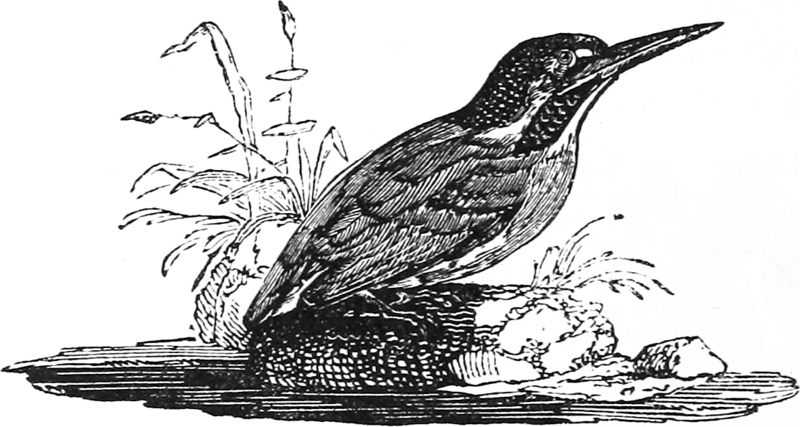
\includegraphics[scale=0.35]{images/Alycon.png}
        \end{figure}
        \vspace{0.5cm}
        \Huge
        \textbf{\textsc{Matematyka Dyskretna}}
        
        \vspace{0.5cm}
        \Large
        \textsc{Wybrane Dowody}
        
        \normalsize
        
        
        \line(1,0){330}
        
        \vspace{1cm}
        \textit{,,Myślę, że 7 punktów na 20 to nie jest zły wynik''}
        \vspace{1cm}

        \textit{\textsc{Popełnione przez}}\\
        \vspace{5mm}

        \textbf{\textsc{Dziurawy Ponton \\ Załatany Ponton \\ Puchaty Pompon \\ Zatopiony Ponton \\ Tonący Ponton \\ Notnop}}

        \vfill

        Kraków \\
        Anno Domini 2023
        
    \end{center}
    
\end{titlepage}


\tableofcontents
\section*{Licencja}
    \begin{figure}[h]
    	\begin{minipage}[c]{0.25\textwidth}
    		
\includegraphics[width=0.7\textwidth]{images/licencja.png}
    	\end{minipage}\hfill
    	\begin{minipage}[c]{0.75\textwidth}
    		\caption*{
    			Ten utwór jest dostępny na 
    			\href{https://creativecommons.org/licenses/by-sa/4.0/}{licencji Creative Commons Uznanie autorstwa
    			na tych samych warunkach 4.0 Międzynarodowe.}
    		}
    	\end{minipage}
    \end{figure}

% Actual content
\mainmatter

\chapter{Kombinatoryka}
 % Żeby nie było syfu to kolejne sekcje dodajemy do chapters/
% A potem includujemy za pomocą \input{chapters/...}

% Używamy \( \) i \[ \] zamiast dolarów -- tak jak się robi w LaTeXu


\documentclass[12pt, a4paper, polish, openany]{book}

% Please, let's familiarize ourselves with notatki.sty and tcs.sty so that we don't reinvent the wheel
\usepackage{notatki}

\fancyhead[L]{\textbf{\textit{MD}}}
\author{
}
\title{TCS and shitposting}


\begin{document}

% Front page and table of contents
\frontmatter

\input{titlepage}

\tableofcontents
\input{license}

% Actual content
\mainmatter

\chapter{Kombinatoryka}
\input{chapters/combinatorics/main}

\chapter{Zasada włączeń i wyłączeń}
\input{chapters/exclusion-inclusion/main}

\chapter{Posety}
\input{chapters/posets/main}

\chapter{Twierdzenie Ramseya}
\input{chapters/ramsey/main}

\chapter{Funkcje tworzące}
\input{chapters/generating_functions/main}

\chapter{Przepływy}
\input{chapters/flows/main}

\chapter{Skojarzenia}
\input{chapters/matchings/main}

\chapter{Kolorowanie grafów}
\input{chapters/graph-coloring/main}

\chapter{Grafy, ale nie kolorowanie}
\input{chapters/graph-misc/main}

\end{document}

\chapter{Zasada włączeń i wyłączeń}
 % Żeby nie było syfu to kolejne sekcje dodajemy do chapters/
% A potem includujemy za pomocą \input{chapters/...}

% Używamy \( \) i \[ \] zamiast dolarów -- tak jak się robi w LaTeXu


\documentclass[12pt, a4paper, polish, openany]{book}

% Please, let's familiarize ourselves with notatki.sty and tcs.sty so that we don't reinvent the wheel
\usepackage{notatki}

\fancyhead[L]{\textbf{\textit{MD}}}
\author{
}
\title{TCS and shitposting}


\begin{document}

% Front page and table of contents
\frontmatter

\input{titlepage}

\tableofcontents
\input{license}

% Actual content
\mainmatter

\chapter{Kombinatoryka}
\input{chapters/combinatorics/main}

\chapter{Zasada włączeń i wyłączeń}
\input{chapters/exclusion-inclusion/main}

\chapter{Posety}
\input{chapters/posets/main}

\chapter{Twierdzenie Ramseya}
\input{chapters/ramsey/main}

\chapter{Funkcje tworzące}
\input{chapters/generating_functions/main}

\chapter{Przepływy}
\input{chapters/flows/main}

\chapter{Skojarzenia}
\input{chapters/matchings/main}

\chapter{Kolorowanie grafów}
\input{chapters/graph-coloring/main}

\chapter{Grafy, ale nie kolorowanie}
\input{chapters/graph-misc/main}

\end{document}

\chapter{Posety}
 % Żeby nie było syfu to kolejne sekcje dodajemy do chapters/
% A potem includujemy za pomocą \input{chapters/...}

% Używamy \( \) i \[ \] zamiast dolarów -- tak jak się robi w LaTeXu


\documentclass[12pt, a4paper, polish, openany]{book}

% Please, let's familiarize ourselves with notatki.sty and tcs.sty so that we don't reinvent the wheel
\usepackage{notatki}

\fancyhead[L]{\textbf{\textit{MD}}}
\author{
}
\title{TCS and shitposting}


\begin{document}

% Front page and table of contents
\frontmatter

\input{titlepage}

\tableofcontents
\input{license}

% Actual content
\mainmatter

\chapter{Kombinatoryka}
\input{chapters/combinatorics/main}

\chapter{Zasada włączeń i wyłączeń}
\input{chapters/exclusion-inclusion/main}

\chapter{Posety}
\input{chapters/posets/main}

\chapter{Twierdzenie Ramseya}
\input{chapters/ramsey/main}

\chapter{Funkcje tworzące}
\input{chapters/generating_functions/main}

\chapter{Przepływy}
\input{chapters/flows/main}

\chapter{Skojarzenia}
\input{chapters/matchings/main}

\chapter{Kolorowanie grafów}
\input{chapters/graph-coloring/main}

\chapter{Grafy, ale nie kolorowanie}
\input{chapters/graph-misc/main}

\end{document}

\chapter{Twierdzenie Ramseya}
 % Żeby nie było syfu to kolejne sekcje dodajemy do chapters/
% A potem includujemy za pomocą \input{chapters/...}

% Używamy \( \) i \[ \] zamiast dolarów -- tak jak się robi w LaTeXu


\documentclass[12pt, a4paper, polish, openany]{book}

% Please, let's familiarize ourselves with notatki.sty and tcs.sty so that we don't reinvent the wheel
\usepackage{notatki}

\fancyhead[L]{\textbf{\textit{MD}}}
\author{
}
\title{TCS and shitposting}


\begin{document}

% Front page and table of contents
\frontmatter

\input{titlepage}

\tableofcontents
\input{license}

% Actual content
\mainmatter

\chapter{Kombinatoryka}
\input{chapters/combinatorics/main}

\chapter{Zasada włączeń i wyłączeń}
\input{chapters/exclusion-inclusion/main}

\chapter{Posety}
\input{chapters/posets/main}

\chapter{Twierdzenie Ramseya}
\input{chapters/ramsey/main}

\chapter{Funkcje tworzące}
\input{chapters/generating_functions/main}

\chapter{Przepływy}
\input{chapters/flows/main}

\chapter{Skojarzenia}
\input{chapters/matchings/main}

\chapter{Kolorowanie grafów}
\input{chapters/graph-coloring/main}

\chapter{Grafy, ale nie kolorowanie}
\input{chapters/graph-misc/main}

\end{document}

\chapter{Funkcje tworzące}
 % Żeby nie było syfu to kolejne sekcje dodajemy do chapters/
% A potem includujemy za pomocą \input{chapters/...}

% Używamy \( \) i \[ \] zamiast dolarów -- tak jak się robi w LaTeXu


\documentclass[12pt, a4paper, polish, openany]{book}

% Please, let's familiarize ourselves with notatki.sty and tcs.sty so that we don't reinvent the wheel
\usepackage{notatki}

\fancyhead[L]{\textbf{\textit{MD}}}
\author{
}
\title{TCS and shitposting}


\begin{document}

% Front page and table of contents
\frontmatter

\input{titlepage}

\tableofcontents
\input{license}

% Actual content
\mainmatter

\chapter{Kombinatoryka}
\input{chapters/combinatorics/main}

\chapter{Zasada włączeń i wyłączeń}
\input{chapters/exclusion-inclusion/main}

\chapter{Posety}
\input{chapters/posets/main}

\chapter{Twierdzenie Ramseya}
\input{chapters/ramsey/main}

\chapter{Funkcje tworzące}
\input{chapters/generating_functions/main}

\chapter{Przepływy}
\input{chapters/flows/main}

\chapter{Skojarzenia}
\input{chapters/matchings/main}

\chapter{Kolorowanie grafów}
\input{chapters/graph-coloring/main}

\chapter{Grafy, ale nie kolorowanie}
\input{chapters/graph-misc/main}

\end{document}

\chapter{Przepływy}
 % Żeby nie było syfu to kolejne sekcje dodajemy do chapters/
% A potem includujemy za pomocą \input{chapters/...}

% Używamy \( \) i \[ \] zamiast dolarów -- tak jak się robi w LaTeXu


\documentclass[12pt, a4paper, polish, openany]{book}

% Please, let's familiarize ourselves with notatki.sty and tcs.sty so that we don't reinvent the wheel
\usepackage{notatki}

\fancyhead[L]{\textbf{\textit{MD}}}
\author{
}
\title{TCS and shitposting}


\begin{document}

% Front page and table of contents
\frontmatter

\input{titlepage}

\tableofcontents
\input{license}

% Actual content
\mainmatter

\chapter{Kombinatoryka}
\input{chapters/combinatorics/main}

\chapter{Zasada włączeń i wyłączeń}
\input{chapters/exclusion-inclusion/main}

\chapter{Posety}
\input{chapters/posets/main}

\chapter{Twierdzenie Ramseya}
\input{chapters/ramsey/main}

\chapter{Funkcje tworzące}
\input{chapters/generating_functions/main}

\chapter{Przepływy}
\input{chapters/flows/main}

\chapter{Skojarzenia}
\input{chapters/matchings/main}

\chapter{Kolorowanie grafów}
\input{chapters/graph-coloring/main}

\chapter{Grafy, ale nie kolorowanie}
\input{chapters/graph-misc/main}

\end{document}

\chapter{Skojarzenia}
 % Żeby nie było syfu to kolejne sekcje dodajemy do chapters/
% A potem includujemy za pomocą \input{chapters/...}

% Używamy \( \) i \[ \] zamiast dolarów -- tak jak się robi w LaTeXu


\documentclass[12pt, a4paper, polish, openany]{book}

% Please, let's familiarize ourselves with notatki.sty and tcs.sty so that we don't reinvent the wheel
\usepackage{notatki}

\fancyhead[L]{\textbf{\textit{MD}}}
\author{
}
\title{TCS and shitposting}


\begin{document}

% Front page and table of contents
\frontmatter

\input{titlepage}

\tableofcontents
\input{license}

% Actual content
\mainmatter

\chapter{Kombinatoryka}
\input{chapters/combinatorics/main}

\chapter{Zasada włączeń i wyłączeń}
\input{chapters/exclusion-inclusion/main}

\chapter{Posety}
\input{chapters/posets/main}

\chapter{Twierdzenie Ramseya}
\input{chapters/ramsey/main}

\chapter{Funkcje tworzące}
\input{chapters/generating_functions/main}

\chapter{Przepływy}
\input{chapters/flows/main}

\chapter{Skojarzenia}
\input{chapters/matchings/main}

\chapter{Kolorowanie grafów}
\input{chapters/graph-coloring/main}

\chapter{Grafy, ale nie kolorowanie}
\input{chapters/graph-misc/main}

\end{document}

\chapter{Kolorowanie grafów}
 % Żeby nie było syfu to kolejne sekcje dodajemy do chapters/
% A potem includujemy za pomocą \input{chapters/...}

% Używamy \( \) i \[ \] zamiast dolarów -- tak jak się robi w LaTeXu


\documentclass[12pt, a4paper, polish, openany]{book}

% Please, let's familiarize ourselves with notatki.sty and tcs.sty so that we don't reinvent the wheel
\usepackage{notatki}

\fancyhead[L]{\textbf{\textit{MD}}}
\author{
}
\title{TCS and shitposting}


\begin{document}

% Front page and table of contents
\frontmatter

\input{titlepage}

\tableofcontents
\input{license}

% Actual content
\mainmatter

\chapter{Kombinatoryka}
\input{chapters/combinatorics/main}

\chapter{Zasada włączeń i wyłączeń}
\input{chapters/exclusion-inclusion/main}

\chapter{Posety}
\input{chapters/posets/main}

\chapter{Twierdzenie Ramseya}
\input{chapters/ramsey/main}

\chapter{Funkcje tworzące}
\input{chapters/generating_functions/main}

\chapter{Przepływy}
\input{chapters/flows/main}

\chapter{Skojarzenia}
\input{chapters/matchings/main}

\chapter{Kolorowanie grafów}
\input{chapters/graph-coloring/main}

\chapter{Grafy, ale nie kolorowanie}
\input{chapters/graph-misc/main}

\end{document}

\chapter{Grafy, ale nie kolorowanie}
 % Żeby nie było syfu to kolejne sekcje dodajemy do chapters/
% A potem includujemy za pomocą \input{chapters/...}

% Używamy \( \) i \[ \] zamiast dolarów -- tak jak się robi w LaTeXu


\documentclass[12pt, a4paper, polish, openany]{book}

% Please, let's familiarize ourselves with notatki.sty and tcs.sty so that we don't reinvent the wheel
\usepackage{notatki}

\fancyhead[L]{\textbf{\textit{MD}}}
\author{
}
\title{TCS and shitposting}


\begin{document}

% Front page and table of contents
\frontmatter

\input{titlepage}

\tableofcontents
\input{license}

% Actual content
\mainmatter

\chapter{Kombinatoryka}
\input{chapters/combinatorics/main}

\chapter{Zasada włączeń i wyłączeń}
\input{chapters/exclusion-inclusion/main}

\chapter{Posety}
\input{chapters/posets/main}

\chapter{Twierdzenie Ramseya}
\input{chapters/ramsey/main}

\chapter{Funkcje tworzące}
\input{chapters/generating_functions/main}

\chapter{Przepływy}
\input{chapters/flows/main}

\chapter{Skojarzenia}
\input{chapters/matchings/main}

\chapter{Kolorowanie grafów}
\input{chapters/graph-coloring/main}

\chapter{Grafy, ale nie kolorowanie}
\input{chapters/graph-misc/main}

\end{document}

\end{document}

\chapter{Funkcje tworzące}
 % Żeby nie było syfu to kolejne sekcje dodajemy do chapters/
% A potem includujemy za pomocą \input{chapters/...}

% Używamy \( \) i \[ \] zamiast dolarów -- tak jak się robi w LaTeXu


\documentclass[12pt, a4paper, polish, openany]{book}

% Please, let's familiarize ourselves with notatki.sty and tcs.sty so that we don't reinvent the wheel
\usepackage{notatki}

\fancyhead[L]{\textbf{\textit{MD}}}
\author{
}
\title{TCS and shitposting}


\begin{document}

% Front page and table of contents
\frontmatter

\begin{titlepage} 

    \begin{center}
         \begin{figure}[h]
            \centering
            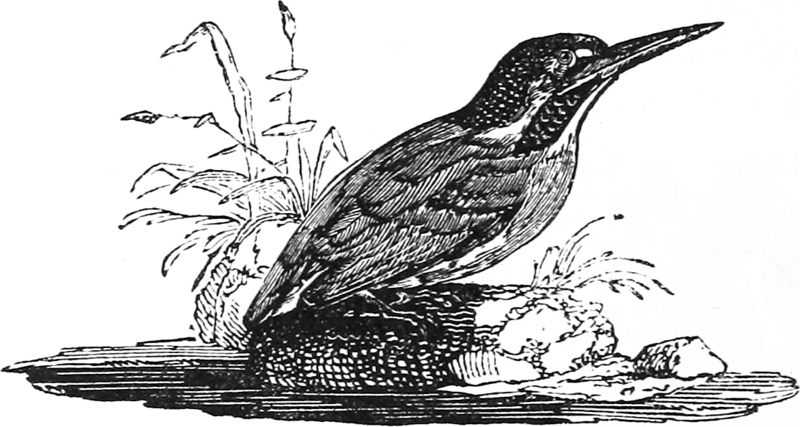
\includegraphics[scale=0.35]{images/Alycon.png}
        \end{figure}
        \vspace{0.5cm}
        \Huge
        \textbf{\textsc{Matematyka Dyskretna}}
        
        \vspace{0.5cm}
        \Large
        \textsc{Wybrane Dowody}
        
        \normalsize
        
        
        \line(1,0){330}
        
        \vspace{1cm}
        \textit{,,Myślę, że 7 punktów na 20 to nie jest zły wynik''}
        \vspace{1cm}

        \textit{\textsc{Popełnione przez}}\\
        \vspace{5mm}

        \textbf{\textsc{Dziurawy Ponton \\ Załatany Ponton \\ Puchaty Pompon \\ Zatopiony Ponton \\ Tonący Ponton \\ Notnop}}

        \vfill

        Kraków \\
        Anno Domini 2023
        
    \end{center}
    
\end{titlepage}


\tableofcontents
\section*{Licencja}
    \begin{figure}[h]
    	\begin{minipage}[c]{0.25\textwidth}
    		
\includegraphics[width=0.7\textwidth]{images/licencja.png}
    	\end{minipage}\hfill
    	\begin{minipage}[c]{0.75\textwidth}
    		\caption*{
    			Ten utwór jest dostępny na 
    			\href{https://creativecommons.org/licenses/by-sa/4.0/}{licencji Creative Commons Uznanie autorstwa
    			na tych samych warunkach 4.0 Międzynarodowe.}
    		}
    	\end{minipage}
    \end{figure}

% Actual content
\mainmatter

\chapter{Kombinatoryka}
 % Żeby nie było syfu to kolejne sekcje dodajemy do chapters/
% A potem includujemy za pomocą \input{chapters/...}

% Używamy \( \) i \[ \] zamiast dolarów -- tak jak się robi w LaTeXu


\documentclass[12pt, a4paper, polish, openany]{book}

% Please, let's familiarize ourselves with notatki.sty and tcs.sty so that we don't reinvent the wheel
\usepackage{notatki}

\fancyhead[L]{\textbf{\textit{MD}}}
\author{
}
\title{TCS and shitposting}


\begin{document}

% Front page and table of contents
\frontmatter

\input{titlepage}

\tableofcontents
\input{license}

% Actual content
\mainmatter

\chapter{Kombinatoryka}
\input{chapters/combinatorics/main}

\chapter{Zasada włączeń i wyłączeń}
\input{chapters/exclusion-inclusion/main}

\chapter{Posety}
\input{chapters/posets/main}

\chapter{Twierdzenie Ramseya}
\input{chapters/ramsey/main}

\chapter{Funkcje tworzące}
\input{chapters/generating_functions/main}

\chapter{Przepływy}
\input{chapters/flows/main}

\chapter{Skojarzenia}
\input{chapters/matchings/main}

\chapter{Kolorowanie grafów}
\input{chapters/graph-coloring/main}

\chapter{Grafy, ale nie kolorowanie}
\input{chapters/graph-misc/main}

\end{document}

\chapter{Zasada włączeń i wyłączeń}
 % Żeby nie było syfu to kolejne sekcje dodajemy do chapters/
% A potem includujemy za pomocą \input{chapters/...}

% Używamy \( \) i \[ \] zamiast dolarów -- tak jak się robi w LaTeXu


\documentclass[12pt, a4paper, polish, openany]{book}

% Please, let's familiarize ourselves with notatki.sty and tcs.sty so that we don't reinvent the wheel
\usepackage{notatki}

\fancyhead[L]{\textbf{\textit{MD}}}
\author{
}
\title{TCS and shitposting}


\begin{document}

% Front page and table of contents
\frontmatter

\input{titlepage}

\tableofcontents
\input{license}

% Actual content
\mainmatter

\chapter{Kombinatoryka}
\input{chapters/combinatorics/main}

\chapter{Zasada włączeń i wyłączeń}
\input{chapters/exclusion-inclusion/main}

\chapter{Posety}
\input{chapters/posets/main}

\chapter{Twierdzenie Ramseya}
\input{chapters/ramsey/main}

\chapter{Funkcje tworzące}
\input{chapters/generating_functions/main}

\chapter{Przepływy}
\input{chapters/flows/main}

\chapter{Skojarzenia}
\input{chapters/matchings/main}

\chapter{Kolorowanie grafów}
\input{chapters/graph-coloring/main}

\chapter{Grafy, ale nie kolorowanie}
\input{chapters/graph-misc/main}

\end{document}

\chapter{Posety}
 % Żeby nie było syfu to kolejne sekcje dodajemy do chapters/
% A potem includujemy za pomocą \input{chapters/...}

% Używamy \( \) i \[ \] zamiast dolarów -- tak jak się robi w LaTeXu


\documentclass[12pt, a4paper, polish, openany]{book}

% Please, let's familiarize ourselves with notatki.sty and tcs.sty so that we don't reinvent the wheel
\usepackage{notatki}

\fancyhead[L]{\textbf{\textit{MD}}}
\author{
}
\title{TCS and shitposting}


\begin{document}

% Front page and table of contents
\frontmatter

\input{titlepage}

\tableofcontents
\input{license}

% Actual content
\mainmatter

\chapter{Kombinatoryka}
\input{chapters/combinatorics/main}

\chapter{Zasada włączeń i wyłączeń}
\input{chapters/exclusion-inclusion/main}

\chapter{Posety}
\input{chapters/posets/main}

\chapter{Twierdzenie Ramseya}
\input{chapters/ramsey/main}

\chapter{Funkcje tworzące}
\input{chapters/generating_functions/main}

\chapter{Przepływy}
\input{chapters/flows/main}

\chapter{Skojarzenia}
\input{chapters/matchings/main}

\chapter{Kolorowanie grafów}
\input{chapters/graph-coloring/main}

\chapter{Grafy, ale nie kolorowanie}
\input{chapters/graph-misc/main}

\end{document}

\chapter{Twierdzenie Ramseya}
 % Żeby nie było syfu to kolejne sekcje dodajemy do chapters/
% A potem includujemy za pomocą \input{chapters/...}

% Używamy \( \) i \[ \] zamiast dolarów -- tak jak się robi w LaTeXu


\documentclass[12pt, a4paper, polish, openany]{book}

% Please, let's familiarize ourselves with notatki.sty and tcs.sty so that we don't reinvent the wheel
\usepackage{notatki}

\fancyhead[L]{\textbf{\textit{MD}}}
\author{
}
\title{TCS and shitposting}


\begin{document}

% Front page and table of contents
\frontmatter

\input{titlepage}

\tableofcontents
\input{license}

% Actual content
\mainmatter

\chapter{Kombinatoryka}
\input{chapters/combinatorics/main}

\chapter{Zasada włączeń i wyłączeń}
\input{chapters/exclusion-inclusion/main}

\chapter{Posety}
\input{chapters/posets/main}

\chapter{Twierdzenie Ramseya}
\input{chapters/ramsey/main}

\chapter{Funkcje tworzące}
\input{chapters/generating_functions/main}

\chapter{Przepływy}
\input{chapters/flows/main}

\chapter{Skojarzenia}
\input{chapters/matchings/main}

\chapter{Kolorowanie grafów}
\input{chapters/graph-coloring/main}

\chapter{Grafy, ale nie kolorowanie}
\input{chapters/graph-misc/main}

\end{document}

\chapter{Funkcje tworzące}
 % Żeby nie było syfu to kolejne sekcje dodajemy do chapters/
% A potem includujemy za pomocą \input{chapters/...}

% Używamy \( \) i \[ \] zamiast dolarów -- tak jak się robi w LaTeXu


\documentclass[12pt, a4paper, polish, openany]{book}

% Please, let's familiarize ourselves with notatki.sty and tcs.sty so that we don't reinvent the wheel
\usepackage{notatki}

\fancyhead[L]{\textbf{\textit{MD}}}
\author{
}
\title{TCS and shitposting}


\begin{document}

% Front page and table of contents
\frontmatter

\input{titlepage}

\tableofcontents
\input{license}

% Actual content
\mainmatter

\chapter{Kombinatoryka}
\input{chapters/combinatorics/main}

\chapter{Zasada włączeń i wyłączeń}
\input{chapters/exclusion-inclusion/main}

\chapter{Posety}
\input{chapters/posets/main}

\chapter{Twierdzenie Ramseya}
\input{chapters/ramsey/main}

\chapter{Funkcje tworzące}
\input{chapters/generating_functions/main}

\chapter{Przepływy}
\input{chapters/flows/main}

\chapter{Skojarzenia}
\input{chapters/matchings/main}

\chapter{Kolorowanie grafów}
\input{chapters/graph-coloring/main}

\chapter{Grafy, ale nie kolorowanie}
\input{chapters/graph-misc/main}

\end{document}

\chapter{Przepływy}
 % Żeby nie było syfu to kolejne sekcje dodajemy do chapters/
% A potem includujemy za pomocą \input{chapters/...}

% Używamy \( \) i \[ \] zamiast dolarów -- tak jak się robi w LaTeXu


\documentclass[12pt, a4paper, polish, openany]{book}

% Please, let's familiarize ourselves with notatki.sty and tcs.sty so that we don't reinvent the wheel
\usepackage{notatki}

\fancyhead[L]{\textbf{\textit{MD}}}
\author{
}
\title{TCS and shitposting}


\begin{document}

% Front page and table of contents
\frontmatter

\input{titlepage}

\tableofcontents
\input{license}

% Actual content
\mainmatter

\chapter{Kombinatoryka}
\input{chapters/combinatorics/main}

\chapter{Zasada włączeń i wyłączeń}
\input{chapters/exclusion-inclusion/main}

\chapter{Posety}
\input{chapters/posets/main}

\chapter{Twierdzenie Ramseya}
\input{chapters/ramsey/main}

\chapter{Funkcje tworzące}
\input{chapters/generating_functions/main}

\chapter{Przepływy}
\input{chapters/flows/main}

\chapter{Skojarzenia}
\input{chapters/matchings/main}

\chapter{Kolorowanie grafów}
\input{chapters/graph-coloring/main}

\chapter{Grafy, ale nie kolorowanie}
\input{chapters/graph-misc/main}

\end{document}

\chapter{Skojarzenia}
 % Żeby nie było syfu to kolejne sekcje dodajemy do chapters/
% A potem includujemy za pomocą \input{chapters/...}

% Używamy \( \) i \[ \] zamiast dolarów -- tak jak się robi w LaTeXu


\documentclass[12pt, a4paper, polish, openany]{book}

% Please, let's familiarize ourselves with notatki.sty and tcs.sty so that we don't reinvent the wheel
\usepackage{notatki}

\fancyhead[L]{\textbf{\textit{MD}}}
\author{
}
\title{TCS and shitposting}


\begin{document}

% Front page and table of contents
\frontmatter

\input{titlepage}

\tableofcontents
\input{license}

% Actual content
\mainmatter

\chapter{Kombinatoryka}
\input{chapters/combinatorics/main}

\chapter{Zasada włączeń i wyłączeń}
\input{chapters/exclusion-inclusion/main}

\chapter{Posety}
\input{chapters/posets/main}

\chapter{Twierdzenie Ramseya}
\input{chapters/ramsey/main}

\chapter{Funkcje tworzące}
\input{chapters/generating_functions/main}

\chapter{Przepływy}
\input{chapters/flows/main}

\chapter{Skojarzenia}
\input{chapters/matchings/main}

\chapter{Kolorowanie grafów}
\input{chapters/graph-coloring/main}

\chapter{Grafy, ale nie kolorowanie}
\input{chapters/graph-misc/main}

\end{document}

\chapter{Kolorowanie grafów}
 % Żeby nie było syfu to kolejne sekcje dodajemy do chapters/
% A potem includujemy za pomocą \input{chapters/...}

% Używamy \( \) i \[ \] zamiast dolarów -- tak jak się robi w LaTeXu


\documentclass[12pt, a4paper, polish, openany]{book}

% Please, let's familiarize ourselves with notatki.sty and tcs.sty so that we don't reinvent the wheel
\usepackage{notatki}

\fancyhead[L]{\textbf{\textit{MD}}}
\author{
}
\title{TCS and shitposting}


\begin{document}

% Front page and table of contents
\frontmatter

\input{titlepage}

\tableofcontents
\input{license}

% Actual content
\mainmatter

\chapter{Kombinatoryka}
\input{chapters/combinatorics/main}

\chapter{Zasada włączeń i wyłączeń}
\input{chapters/exclusion-inclusion/main}

\chapter{Posety}
\input{chapters/posets/main}

\chapter{Twierdzenie Ramseya}
\input{chapters/ramsey/main}

\chapter{Funkcje tworzące}
\input{chapters/generating_functions/main}

\chapter{Przepływy}
\input{chapters/flows/main}

\chapter{Skojarzenia}
\input{chapters/matchings/main}

\chapter{Kolorowanie grafów}
\input{chapters/graph-coloring/main}

\chapter{Grafy, ale nie kolorowanie}
\input{chapters/graph-misc/main}

\end{document}

\chapter{Grafy, ale nie kolorowanie}
 % Żeby nie było syfu to kolejne sekcje dodajemy do chapters/
% A potem includujemy za pomocą \input{chapters/...}

% Używamy \( \) i \[ \] zamiast dolarów -- tak jak się robi w LaTeXu


\documentclass[12pt, a4paper, polish, openany]{book}

% Please, let's familiarize ourselves with notatki.sty and tcs.sty so that we don't reinvent the wheel
\usepackage{notatki}

\fancyhead[L]{\textbf{\textit{MD}}}
\author{
}
\title{TCS and shitposting}


\begin{document}

% Front page and table of contents
\frontmatter

\input{titlepage}

\tableofcontents
\input{license}

% Actual content
\mainmatter

\chapter{Kombinatoryka}
\input{chapters/combinatorics/main}

\chapter{Zasada włączeń i wyłączeń}
\input{chapters/exclusion-inclusion/main}

\chapter{Posety}
\input{chapters/posets/main}

\chapter{Twierdzenie Ramseya}
\input{chapters/ramsey/main}

\chapter{Funkcje tworzące}
\input{chapters/generating_functions/main}

\chapter{Przepływy}
\input{chapters/flows/main}

\chapter{Skojarzenia}
\input{chapters/matchings/main}

\chapter{Kolorowanie grafów}
\input{chapters/graph-coloring/main}

\chapter{Grafy, ale nie kolorowanie}
\input{chapters/graph-misc/main}

\end{document}

\end{document}

\chapter{Przepływy}
 % Żeby nie było syfu to kolejne sekcje dodajemy do chapters/
% A potem includujemy za pomocą \input{chapters/...}

% Używamy \( \) i \[ \] zamiast dolarów -- tak jak się robi w LaTeXu


\documentclass[12pt, a4paper, polish, openany]{book}

% Please, let's familiarize ourselves with notatki.sty and tcs.sty so that we don't reinvent the wheel
\usepackage{notatki}

\fancyhead[L]{\textbf{\textit{MD}}}
\author{
}
\title{TCS and shitposting}


\begin{document}

% Front page and table of contents
\frontmatter

\begin{titlepage} 

    \begin{center}
         \begin{figure}[h]
            \centering
            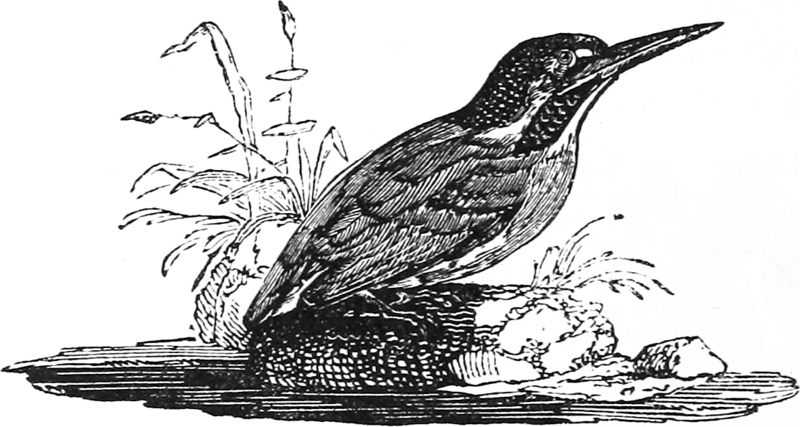
\includegraphics[scale=0.35]{images/Alycon.png}
        \end{figure}
        \vspace{0.5cm}
        \Huge
        \textbf{\textsc{Matematyka Dyskretna}}
        
        \vspace{0.5cm}
        \Large
        \textsc{Wybrane Dowody}
        
        \normalsize
        
        
        \line(1,0){330}
        
        \vspace{1cm}
        \textit{,,Myślę, że 7 punktów na 20 to nie jest zły wynik''}
        \vspace{1cm}

        \textit{\textsc{Popełnione przez}}\\
        \vspace{5mm}

        \textbf{\textsc{Dziurawy Ponton \\ Załatany Ponton \\ Puchaty Pompon \\ Zatopiony Ponton \\ Tonący Ponton \\ Notnop}}

        \vfill

        Kraków \\
        Anno Domini 2023
        
    \end{center}
    
\end{titlepage}


\tableofcontents
\section*{Licencja}
    \begin{figure}[h]
    	\begin{minipage}[c]{0.25\textwidth}
    		
\includegraphics[width=0.7\textwidth]{images/licencja.png}
    	\end{minipage}\hfill
    	\begin{minipage}[c]{0.75\textwidth}
    		\caption*{
    			Ten utwór jest dostępny na 
    			\href{https://creativecommons.org/licenses/by-sa/4.0/}{licencji Creative Commons Uznanie autorstwa
    			na tych samych warunkach 4.0 Międzynarodowe.}
    		}
    	\end{minipage}
    \end{figure}

% Actual content
\mainmatter

\chapter{Kombinatoryka}
 % Żeby nie było syfu to kolejne sekcje dodajemy do chapters/
% A potem includujemy za pomocą \input{chapters/...}

% Używamy \( \) i \[ \] zamiast dolarów -- tak jak się robi w LaTeXu


\documentclass[12pt, a4paper, polish, openany]{book}

% Please, let's familiarize ourselves with notatki.sty and tcs.sty so that we don't reinvent the wheel
\usepackage{notatki}

\fancyhead[L]{\textbf{\textit{MD}}}
\author{
}
\title{TCS and shitposting}


\begin{document}

% Front page and table of contents
\frontmatter

\input{titlepage}

\tableofcontents
\input{license}

% Actual content
\mainmatter

\chapter{Kombinatoryka}
\input{chapters/combinatorics/main}

\chapter{Zasada włączeń i wyłączeń}
\input{chapters/exclusion-inclusion/main}

\chapter{Posety}
\input{chapters/posets/main}

\chapter{Twierdzenie Ramseya}
\input{chapters/ramsey/main}

\chapter{Funkcje tworzące}
\input{chapters/generating_functions/main}

\chapter{Przepływy}
\input{chapters/flows/main}

\chapter{Skojarzenia}
\input{chapters/matchings/main}

\chapter{Kolorowanie grafów}
\input{chapters/graph-coloring/main}

\chapter{Grafy, ale nie kolorowanie}
\input{chapters/graph-misc/main}

\end{document}

\chapter{Zasada włączeń i wyłączeń}
 % Żeby nie było syfu to kolejne sekcje dodajemy do chapters/
% A potem includujemy za pomocą \input{chapters/...}

% Używamy \( \) i \[ \] zamiast dolarów -- tak jak się robi w LaTeXu


\documentclass[12pt, a4paper, polish, openany]{book}

% Please, let's familiarize ourselves with notatki.sty and tcs.sty so that we don't reinvent the wheel
\usepackage{notatki}

\fancyhead[L]{\textbf{\textit{MD}}}
\author{
}
\title{TCS and shitposting}


\begin{document}

% Front page and table of contents
\frontmatter

\input{titlepage}

\tableofcontents
\input{license}

% Actual content
\mainmatter

\chapter{Kombinatoryka}
\input{chapters/combinatorics/main}

\chapter{Zasada włączeń i wyłączeń}
\input{chapters/exclusion-inclusion/main}

\chapter{Posety}
\input{chapters/posets/main}

\chapter{Twierdzenie Ramseya}
\input{chapters/ramsey/main}

\chapter{Funkcje tworzące}
\input{chapters/generating_functions/main}

\chapter{Przepływy}
\input{chapters/flows/main}

\chapter{Skojarzenia}
\input{chapters/matchings/main}

\chapter{Kolorowanie grafów}
\input{chapters/graph-coloring/main}

\chapter{Grafy, ale nie kolorowanie}
\input{chapters/graph-misc/main}

\end{document}

\chapter{Posety}
 % Żeby nie było syfu to kolejne sekcje dodajemy do chapters/
% A potem includujemy za pomocą \input{chapters/...}

% Używamy \( \) i \[ \] zamiast dolarów -- tak jak się robi w LaTeXu


\documentclass[12pt, a4paper, polish, openany]{book}

% Please, let's familiarize ourselves with notatki.sty and tcs.sty so that we don't reinvent the wheel
\usepackage{notatki}

\fancyhead[L]{\textbf{\textit{MD}}}
\author{
}
\title{TCS and shitposting}


\begin{document}

% Front page and table of contents
\frontmatter

\input{titlepage}

\tableofcontents
\input{license}

% Actual content
\mainmatter

\chapter{Kombinatoryka}
\input{chapters/combinatorics/main}

\chapter{Zasada włączeń i wyłączeń}
\input{chapters/exclusion-inclusion/main}

\chapter{Posety}
\input{chapters/posets/main}

\chapter{Twierdzenie Ramseya}
\input{chapters/ramsey/main}

\chapter{Funkcje tworzące}
\input{chapters/generating_functions/main}

\chapter{Przepływy}
\input{chapters/flows/main}

\chapter{Skojarzenia}
\input{chapters/matchings/main}

\chapter{Kolorowanie grafów}
\input{chapters/graph-coloring/main}

\chapter{Grafy, ale nie kolorowanie}
\input{chapters/graph-misc/main}

\end{document}

\chapter{Twierdzenie Ramseya}
 % Żeby nie było syfu to kolejne sekcje dodajemy do chapters/
% A potem includujemy za pomocą \input{chapters/...}

% Używamy \( \) i \[ \] zamiast dolarów -- tak jak się robi w LaTeXu


\documentclass[12pt, a4paper, polish, openany]{book}

% Please, let's familiarize ourselves with notatki.sty and tcs.sty so that we don't reinvent the wheel
\usepackage{notatki}

\fancyhead[L]{\textbf{\textit{MD}}}
\author{
}
\title{TCS and shitposting}


\begin{document}

% Front page and table of contents
\frontmatter

\input{titlepage}

\tableofcontents
\input{license}

% Actual content
\mainmatter

\chapter{Kombinatoryka}
\input{chapters/combinatorics/main}

\chapter{Zasada włączeń i wyłączeń}
\input{chapters/exclusion-inclusion/main}

\chapter{Posety}
\input{chapters/posets/main}

\chapter{Twierdzenie Ramseya}
\input{chapters/ramsey/main}

\chapter{Funkcje tworzące}
\input{chapters/generating_functions/main}

\chapter{Przepływy}
\input{chapters/flows/main}

\chapter{Skojarzenia}
\input{chapters/matchings/main}

\chapter{Kolorowanie grafów}
\input{chapters/graph-coloring/main}

\chapter{Grafy, ale nie kolorowanie}
\input{chapters/graph-misc/main}

\end{document}

\chapter{Funkcje tworzące}
 % Żeby nie było syfu to kolejne sekcje dodajemy do chapters/
% A potem includujemy za pomocą \input{chapters/...}

% Używamy \( \) i \[ \] zamiast dolarów -- tak jak się robi w LaTeXu


\documentclass[12pt, a4paper, polish, openany]{book}

% Please, let's familiarize ourselves with notatki.sty and tcs.sty so that we don't reinvent the wheel
\usepackage{notatki}

\fancyhead[L]{\textbf{\textit{MD}}}
\author{
}
\title{TCS and shitposting}


\begin{document}

% Front page and table of contents
\frontmatter

\input{titlepage}

\tableofcontents
\input{license}

% Actual content
\mainmatter

\chapter{Kombinatoryka}
\input{chapters/combinatorics/main}

\chapter{Zasada włączeń i wyłączeń}
\input{chapters/exclusion-inclusion/main}

\chapter{Posety}
\input{chapters/posets/main}

\chapter{Twierdzenie Ramseya}
\input{chapters/ramsey/main}

\chapter{Funkcje tworzące}
\input{chapters/generating_functions/main}

\chapter{Przepływy}
\input{chapters/flows/main}

\chapter{Skojarzenia}
\input{chapters/matchings/main}

\chapter{Kolorowanie grafów}
\input{chapters/graph-coloring/main}

\chapter{Grafy, ale nie kolorowanie}
\input{chapters/graph-misc/main}

\end{document}

\chapter{Przepływy}
 % Żeby nie było syfu to kolejne sekcje dodajemy do chapters/
% A potem includujemy za pomocą \input{chapters/...}

% Używamy \( \) i \[ \] zamiast dolarów -- tak jak się robi w LaTeXu


\documentclass[12pt, a4paper, polish, openany]{book}

% Please, let's familiarize ourselves with notatki.sty and tcs.sty so that we don't reinvent the wheel
\usepackage{notatki}

\fancyhead[L]{\textbf{\textit{MD}}}
\author{
}
\title{TCS and shitposting}


\begin{document}

% Front page and table of contents
\frontmatter

\input{titlepage}

\tableofcontents
\input{license}

% Actual content
\mainmatter

\chapter{Kombinatoryka}
\input{chapters/combinatorics/main}

\chapter{Zasada włączeń i wyłączeń}
\input{chapters/exclusion-inclusion/main}

\chapter{Posety}
\input{chapters/posets/main}

\chapter{Twierdzenie Ramseya}
\input{chapters/ramsey/main}

\chapter{Funkcje tworzące}
\input{chapters/generating_functions/main}

\chapter{Przepływy}
\input{chapters/flows/main}

\chapter{Skojarzenia}
\input{chapters/matchings/main}

\chapter{Kolorowanie grafów}
\input{chapters/graph-coloring/main}

\chapter{Grafy, ale nie kolorowanie}
\input{chapters/graph-misc/main}

\end{document}

\chapter{Skojarzenia}
 % Żeby nie było syfu to kolejne sekcje dodajemy do chapters/
% A potem includujemy za pomocą \input{chapters/...}

% Używamy \( \) i \[ \] zamiast dolarów -- tak jak się robi w LaTeXu


\documentclass[12pt, a4paper, polish, openany]{book}

% Please, let's familiarize ourselves with notatki.sty and tcs.sty so that we don't reinvent the wheel
\usepackage{notatki}

\fancyhead[L]{\textbf{\textit{MD}}}
\author{
}
\title{TCS and shitposting}


\begin{document}

% Front page and table of contents
\frontmatter

\input{titlepage}

\tableofcontents
\input{license}

% Actual content
\mainmatter

\chapter{Kombinatoryka}
\input{chapters/combinatorics/main}

\chapter{Zasada włączeń i wyłączeń}
\input{chapters/exclusion-inclusion/main}

\chapter{Posety}
\input{chapters/posets/main}

\chapter{Twierdzenie Ramseya}
\input{chapters/ramsey/main}

\chapter{Funkcje tworzące}
\input{chapters/generating_functions/main}

\chapter{Przepływy}
\input{chapters/flows/main}

\chapter{Skojarzenia}
\input{chapters/matchings/main}

\chapter{Kolorowanie grafów}
\input{chapters/graph-coloring/main}

\chapter{Grafy, ale nie kolorowanie}
\input{chapters/graph-misc/main}

\end{document}

\chapter{Kolorowanie grafów}
 % Żeby nie było syfu to kolejne sekcje dodajemy do chapters/
% A potem includujemy za pomocą \input{chapters/...}

% Używamy \( \) i \[ \] zamiast dolarów -- tak jak się robi w LaTeXu


\documentclass[12pt, a4paper, polish, openany]{book}

% Please, let's familiarize ourselves with notatki.sty and tcs.sty so that we don't reinvent the wheel
\usepackage{notatki}

\fancyhead[L]{\textbf{\textit{MD}}}
\author{
}
\title{TCS and shitposting}


\begin{document}

% Front page and table of contents
\frontmatter

\input{titlepage}

\tableofcontents
\input{license}

% Actual content
\mainmatter

\chapter{Kombinatoryka}
\input{chapters/combinatorics/main}

\chapter{Zasada włączeń i wyłączeń}
\input{chapters/exclusion-inclusion/main}

\chapter{Posety}
\input{chapters/posets/main}

\chapter{Twierdzenie Ramseya}
\input{chapters/ramsey/main}

\chapter{Funkcje tworzące}
\input{chapters/generating_functions/main}

\chapter{Przepływy}
\input{chapters/flows/main}

\chapter{Skojarzenia}
\input{chapters/matchings/main}

\chapter{Kolorowanie grafów}
\input{chapters/graph-coloring/main}

\chapter{Grafy, ale nie kolorowanie}
\input{chapters/graph-misc/main}

\end{document}

\chapter{Grafy, ale nie kolorowanie}
 % Żeby nie było syfu to kolejne sekcje dodajemy do chapters/
% A potem includujemy za pomocą \input{chapters/...}

% Używamy \( \) i \[ \] zamiast dolarów -- tak jak się robi w LaTeXu


\documentclass[12pt, a4paper, polish, openany]{book}

% Please, let's familiarize ourselves with notatki.sty and tcs.sty so that we don't reinvent the wheel
\usepackage{notatki}

\fancyhead[L]{\textbf{\textit{MD}}}
\author{
}
\title{TCS and shitposting}


\begin{document}

% Front page and table of contents
\frontmatter

\input{titlepage}

\tableofcontents
\input{license}

% Actual content
\mainmatter

\chapter{Kombinatoryka}
\input{chapters/combinatorics/main}

\chapter{Zasada włączeń i wyłączeń}
\input{chapters/exclusion-inclusion/main}

\chapter{Posety}
\input{chapters/posets/main}

\chapter{Twierdzenie Ramseya}
\input{chapters/ramsey/main}

\chapter{Funkcje tworzące}
\input{chapters/generating_functions/main}

\chapter{Przepływy}
\input{chapters/flows/main}

\chapter{Skojarzenia}
\input{chapters/matchings/main}

\chapter{Kolorowanie grafów}
\input{chapters/graph-coloring/main}

\chapter{Grafy, ale nie kolorowanie}
\input{chapters/graph-misc/main}

\end{document}

\end{document}

\chapter{Skojarzenia}
 % Żeby nie było syfu to kolejne sekcje dodajemy do chapters/
% A potem includujemy za pomocą \input{chapters/...}

% Używamy \( \) i \[ \] zamiast dolarów -- tak jak się robi w LaTeXu


\documentclass[12pt, a4paper, polish, openany]{book}

% Please, let's familiarize ourselves with notatki.sty and tcs.sty so that we don't reinvent the wheel
\usepackage{notatki}

\fancyhead[L]{\textbf{\textit{MD}}}
\author{
}
\title{TCS and shitposting}


\begin{document}

% Front page and table of contents
\frontmatter

\begin{titlepage} 

    \begin{center}
         \begin{figure}[h]
            \centering
            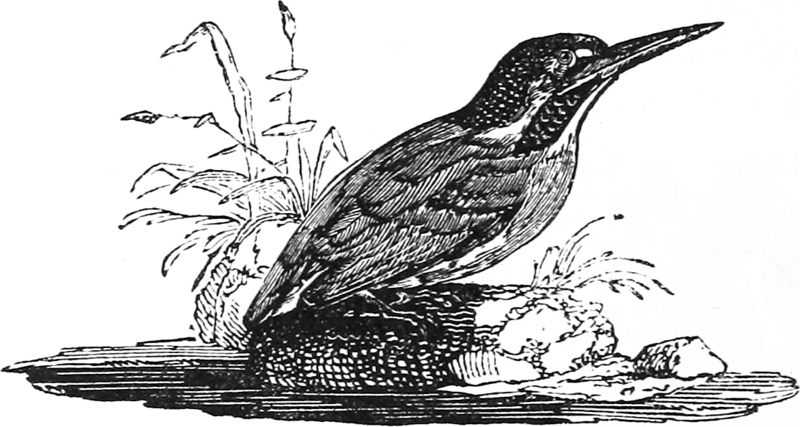
\includegraphics[scale=0.35]{images/Alycon.png}
        \end{figure}
        \vspace{0.5cm}
        \Huge
        \textbf{\textsc{Matematyka Dyskretna}}
        
        \vspace{0.5cm}
        \Large
        \textsc{Wybrane Dowody}
        
        \normalsize
        
        
        \line(1,0){330}
        
        \vspace{1cm}
        \textit{,,Myślę, że 7 punktów na 20 to nie jest zły wynik''}
        \vspace{1cm}

        \textit{\textsc{Popełnione przez}}\\
        \vspace{5mm}

        \textbf{\textsc{Dziurawy Ponton \\ Załatany Ponton \\ Puchaty Pompon \\ Zatopiony Ponton \\ Tonący Ponton \\ Notnop}}

        \vfill

        Kraków \\
        Anno Domini 2023
        
    \end{center}
    
\end{titlepage}


\tableofcontents
\section*{Licencja}
    \begin{figure}[h]
    	\begin{minipage}[c]{0.25\textwidth}
    		
\includegraphics[width=0.7\textwidth]{images/licencja.png}
    	\end{minipage}\hfill
    	\begin{minipage}[c]{0.75\textwidth}
    		\caption*{
    			Ten utwór jest dostępny na 
    			\href{https://creativecommons.org/licenses/by-sa/4.0/}{licencji Creative Commons Uznanie autorstwa
    			na tych samych warunkach 4.0 Międzynarodowe.}
    		}
    	\end{minipage}
    \end{figure}

% Actual content
\mainmatter

\chapter{Kombinatoryka}
 % Żeby nie było syfu to kolejne sekcje dodajemy do chapters/
% A potem includujemy za pomocą \input{chapters/...}

% Używamy \( \) i \[ \] zamiast dolarów -- tak jak się robi w LaTeXu


\documentclass[12pt, a4paper, polish, openany]{book}

% Please, let's familiarize ourselves with notatki.sty and tcs.sty so that we don't reinvent the wheel
\usepackage{notatki}

\fancyhead[L]{\textbf{\textit{MD}}}
\author{
}
\title{TCS and shitposting}


\begin{document}

% Front page and table of contents
\frontmatter

\input{titlepage}

\tableofcontents
\input{license}

% Actual content
\mainmatter

\chapter{Kombinatoryka}
\input{chapters/combinatorics/main}

\chapter{Zasada włączeń i wyłączeń}
\input{chapters/exclusion-inclusion/main}

\chapter{Posety}
\input{chapters/posets/main}

\chapter{Twierdzenie Ramseya}
\input{chapters/ramsey/main}

\chapter{Funkcje tworzące}
\input{chapters/generating_functions/main}

\chapter{Przepływy}
\input{chapters/flows/main}

\chapter{Skojarzenia}
\input{chapters/matchings/main}

\chapter{Kolorowanie grafów}
\input{chapters/graph-coloring/main}

\chapter{Grafy, ale nie kolorowanie}
\input{chapters/graph-misc/main}

\end{document}

\chapter{Zasada włączeń i wyłączeń}
 % Żeby nie było syfu to kolejne sekcje dodajemy do chapters/
% A potem includujemy za pomocą \input{chapters/...}

% Używamy \( \) i \[ \] zamiast dolarów -- tak jak się robi w LaTeXu


\documentclass[12pt, a4paper, polish, openany]{book}

% Please, let's familiarize ourselves with notatki.sty and tcs.sty so that we don't reinvent the wheel
\usepackage{notatki}

\fancyhead[L]{\textbf{\textit{MD}}}
\author{
}
\title{TCS and shitposting}


\begin{document}

% Front page and table of contents
\frontmatter

\input{titlepage}

\tableofcontents
\input{license}

% Actual content
\mainmatter

\chapter{Kombinatoryka}
\input{chapters/combinatorics/main}

\chapter{Zasada włączeń i wyłączeń}
\input{chapters/exclusion-inclusion/main}

\chapter{Posety}
\input{chapters/posets/main}

\chapter{Twierdzenie Ramseya}
\input{chapters/ramsey/main}

\chapter{Funkcje tworzące}
\input{chapters/generating_functions/main}

\chapter{Przepływy}
\input{chapters/flows/main}

\chapter{Skojarzenia}
\input{chapters/matchings/main}

\chapter{Kolorowanie grafów}
\input{chapters/graph-coloring/main}

\chapter{Grafy, ale nie kolorowanie}
\input{chapters/graph-misc/main}

\end{document}

\chapter{Posety}
 % Żeby nie było syfu to kolejne sekcje dodajemy do chapters/
% A potem includujemy za pomocą \input{chapters/...}

% Używamy \( \) i \[ \] zamiast dolarów -- tak jak się robi w LaTeXu


\documentclass[12pt, a4paper, polish, openany]{book}

% Please, let's familiarize ourselves with notatki.sty and tcs.sty so that we don't reinvent the wheel
\usepackage{notatki}

\fancyhead[L]{\textbf{\textit{MD}}}
\author{
}
\title{TCS and shitposting}


\begin{document}

% Front page and table of contents
\frontmatter

\input{titlepage}

\tableofcontents
\input{license}

% Actual content
\mainmatter

\chapter{Kombinatoryka}
\input{chapters/combinatorics/main}

\chapter{Zasada włączeń i wyłączeń}
\input{chapters/exclusion-inclusion/main}

\chapter{Posety}
\input{chapters/posets/main}

\chapter{Twierdzenie Ramseya}
\input{chapters/ramsey/main}

\chapter{Funkcje tworzące}
\input{chapters/generating_functions/main}

\chapter{Przepływy}
\input{chapters/flows/main}

\chapter{Skojarzenia}
\input{chapters/matchings/main}

\chapter{Kolorowanie grafów}
\input{chapters/graph-coloring/main}

\chapter{Grafy, ale nie kolorowanie}
\input{chapters/graph-misc/main}

\end{document}

\chapter{Twierdzenie Ramseya}
 % Żeby nie było syfu to kolejne sekcje dodajemy do chapters/
% A potem includujemy za pomocą \input{chapters/...}

% Używamy \( \) i \[ \] zamiast dolarów -- tak jak się robi w LaTeXu


\documentclass[12pt, a4paper, polish, openany]{book}

% Please, let's familiarize ourselves with notatki.sty and tcs.sty so that we don't reinvent the wheel
\usepackage{notatki}

\fancyhead[L]{\textbf{\textit{MD}}}
\author{
}
\title{TCS and shitposting}


\begin{document}

% Front page and table of contents
\frontmatter

\input{titlepage}

\tableofcontents
\input{license}

% Actual content
\mainmatter

\chapter{Kombinatoryka}
\input{chapters/combinatorics/main}

\chapter{Zasada włączeń i wyłączeń}
\input{chapters/exclusion-inclusion/main}

\chapter{Posety}
\input{chapters/posets/main}

\chapter{Twierdzenie Ramseya}
\input{chapters/ramsey/main}

\chapter{Funkcje tworzące}
\input{chapters/generating_functions/main}

\chapter{Przepływy}
\input{chapters/flows/main}

\chapter{Skojarzenia}
\input{chapters/matchings/main}

\chapter{Kolorowanie grafów}
\input{chapters/graph-coloring/main}

\chapter{Grafy, ale nie kolorowanie}
\input{chapters/graph-misc/main}

\end{document}

\chapter{Funkcje tworzące}
 % Żeby nie było syfu to kolejne sekcje dodajemy do chapters/
% A potem includujemy za pomocą \input{chapters/...}

% Używamy \( \) i \[ \] zamiast dolarów -- tak jak się robi w LaTeXu


\documentclass[12pt, a4paper, polish, openany]{book}

% Please, let's familiarize ourselves with notatki.sty and tcs.sty so that we don't reinvent the wheel
\usepackage{notatki}

\fancyhead[L]{\textbf{\textit{MD}}}
\author{
}
\title{TCS and shitposting}


\begin{document}

% Front page and table of contents
\frontmatter

\input{titlepage}

\tableofcontents
\input{license}

% Actual content
\mainmatter

\chapter{Kombinatoryka}
\input{chapters/combinatorics/main}

\chapter{Zasada włączeń i wyłączeń}
\input{chapters/exclusion-inclusion/main}

\chapter{Posety}
\input{chapters/posets/main}

\chapter{Twierdzenie Ramseya}
\input{chapters/ramsey/main}

\chapter{Funkcje tworzące}
\input{chapters/generating_functions/main}

\chapter{Przepływy}
\input{chapters/flows/main}

\chapter{Skojarzenia}
\input{chapters/matchings/main}

\chapter{Kolorowanie grafów}
\input{chapters/graph-coloring/main}

\chapter{Grafy, ale nie kolorowanie}
\input{chapters/graph-misc/main}

\end{document}

\chapter{Przepływy}
 % Żeby nie było syfu to kolejne sekcje dodajemy do chapters/
% A potem includujemy za pomocą \input{chapters/...}

% Używamy \( \) i \[ \] zamiast dolarów -- tak jak się robi w LaTeXu


\documentclass[12pt, a4paper, polish, openany]{book}

% Please, let's familiarize ourselves with notatki.sty and tcs.sty so that we don't reinvent the wheel
\usepackage{notatki}

\fancyhead[L]{\textbf{\textit{MD}}}
\author{
}
\title{TCS and shitposting}


\begin{document}

% Front page and table of contents
\frontmatter

\input{titlepage}

\tableofcontents
\input{license}

% Actual content
\mainmatter

\chapter{Kombinatoryka}
\input{chapters/combinatorics/main}

\chapter{Zasada włączeń i wyłączeń}
\input{chapters/exclusion-inclusion/main}

\chapter{Posety}
\input{chapters/posets/main}

\chapter{Twierdzenie Ramseya}
\input{chapters/ramsey/main}

\chapter{Funkcje tworzące}
\input{chapters/generating_functions/main}

\chapter{Przepływy}
\input{chapters/flows/main}

\chapter{Skojarzenia}
\input{chapters/matchings/main}

\chapter{Kolorowanie grafów}
\input{chapters/graph-coloring/main}

\chapter{Grafy, ale nie kolorowanie}
\input{chapters/graph-misc/main}

\end{document}

\chapter{Skojarzenia}
 % Żeby nie było syfu to kolejne sekcje dodajemy do chapters/
% A potem includujemy za pomocą \input{chapters/...}

% Używamy \( \) i \[ \] zamiast dolarów -- tak jak się robi w LaTeXu


\documentclass[12pt, a4paper, polish, openany]{book}

% Please, let's familiarize ourselves with notatki.sty and tcs.sty so that we don't reinvent the wheel
\usepackage{notatki}

\fancyhead[L]{\textbf{\textit{MD}}}
\author{
}
\title{TCS and shitposting}


\begin{document}

% Front page and table of contents
\frontmatter

\input{titlepage}

\tableofcontents
\input{license}

% Actual content
\mainmatter

\chapter{Kombinatoryka}
\input{chapters/combinatorics/main}

\chapter{Zasada włączeń i wyłączeń}
\input{chapters/exclusion-inclusion/main}

\chapter{Posety}
\input{chapters/posets/main}

\chapter{Twierdzenie Ramseya}
\input{chapters/ramsey/main}

\chapter{Funkcje tworzące}
\input{chapters/generating_functions/main}

\chapter{Przepływy}
\input{chapters/flows/main}

\chapter{Skojarzenia}
\input{chapters/matchings/main}

\chapter{Kolorowanie grafów}
\input{chapters/graph-coloring/main}

\chapter{Grafy, ale nie kolorowanie}
\input{chapters/graph-misc/main}

\end{document}

\chapter{Kolorowanie grafów}
 % Żeby nie było syfu to kolejne sekcje dodajemy do chapters/
% A potem includujemy za pomocą \input{chapters/...}

% Używamy \( \) i \[ \] zamiast dolarów -- tak jak się robi w LaTeXu


\documentclass[12pt, a4paper, polish, openany]{book}

% Please, let's familiarize ourselves with notatki.sty and tcs.sty so that we don't reinvent the wheel
\usepackage{notatki}

\fancyhead[L]{\textbf{\textit{MD}}}
\author{
}
\title{TCS and shitposting}


\begin{document}

% Front page and table of contents
\frontmatter

\input{titlepage}

\tableofcontents
\input{license}

% Actual content
\mainmatter

\chapter{Kombinatoryka}
\input{chapters/combinatorics/main}

\chapter{Zasada włączeń i wyłączeń}
\input{chapters/exclusion-inclusion/main}

\chapter{Posety}
\input{chapters/posets/main}

\chapter{Twierdzenie Ramseya}
\input{chapters/ramsey/main}

\chapter{Funkcje tworzące}
\input{chapters/generating_functions/main}

\chapter{Przepływy}
\input{chapters/flows/main}

\chapter{Skojarzenia}
\input{chapters/matchings/main}

\chapter{Kolorowanie grafów}
\input{chapters/graph-coloring/main}

\chapter{Grafy, ale nie kolorowanie}
\input{chapters/graph-misc/main}

\end{document}

\chapter{Grafy, ale nie kolorowanie}
 % Żeby nie było syfu to kolejne sekcje dodajemy do chapters/
% A potem includujemy za pomocą \input{chapters/...}

% Używamy \( \) i \[ \] zamiast dolarów -- tak jak się robi w LaTeXu


\documentclass[12pt, a4paper, polish, openany]{book}

% Please, let's familiarize ourselves with notatki.sty and tcs.sty so that we don't reinvent the wheel
\usepackage{notatki}

\fancyhead[L]{\textbf{\textit{MD}}}
\author{
}
\title{TCS and shitposting}


\begin{document}

% Front page and table of contents
\frontmatter

\input{titlepage}

\tableofcontents
\input{license}

% Actual content
\mainmatter

\chapter{Kombinatoryka}
\input{chapters/combinatorics/main}

\chapter{Zasada włączeń i wyłączeń}
\input{chapters/exclusion-inclusion/main}

\chapter{Posety}
\input{chapters/posets/main}

\chapter{Twierdzenie Ramseya}
\input{chapters/ramsey/main}

\chapter{Funkcje tworzące}
\input{chapters/generating_functions/main}

\chapter{Przepływy}
\input{chapters/flows/main}

\chapter{Skojarzenia}
\input{chapters/matchings/main}

\chapter{Kolorowanie grafów}
\input{chapters/graph-coloring/main}

\chapter{Grafy, ale nie kolorowanie}
\input{chapters/graph-misc/main}

\end{document}

\end{document}

\chapter{Kolorowanie grafów}
 % Żeby nie było syfu to kolejne sekcje dodajemy do chapters/
% A potem includujemy za pomocą \input{chapters/...}

% Używamy \( \) i \[ \] zamiast dolarów -- tak jak się robi w LaTeXu


\documentclass[12pt, a4paper, polish, openany]{book}

% Please, let's familiarize ourselves with notatki.sty and tcs.sty so that we don't reinvent the wheel
\usepackage{notatki}

\fancyhead[L]{\textbf{\textit{MD}}}
\author{
}
\title{TCS and shitposting}


\begin{document}

% Front page and table of contents
\frontmatter

\begin{titlepage} 

    \begin{center}
         \begin{figure}[h]
            \centering
            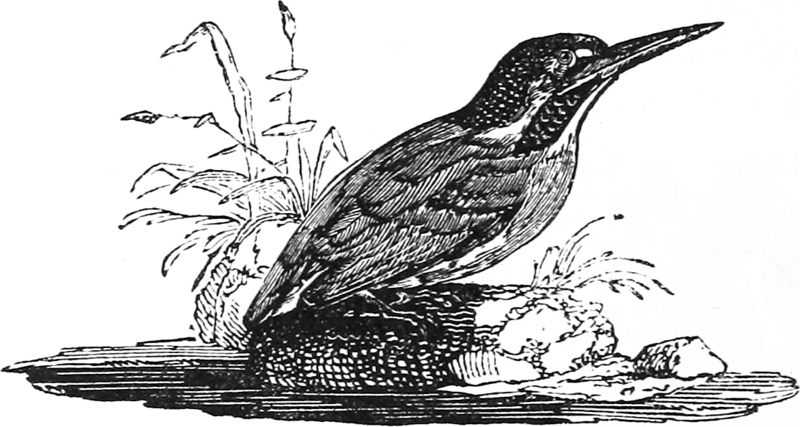
\includegraphics[scale=0.35]{images/Alycon.png}
        \end{figure}
        \vspace{0.5cm}
        \Huge
        \textbf{\textsc{Matematyka Dyskretna}}
        
        \vspace{0.5cm}
        \Large
        \textsc{Wybrane Dowody}
        
        \normalsize
        
        
        \line(1,0){330}
        
        \vspace{1cm}
        \textit{,,Myślę, że 7 punktów na 20 to nie jest zły wynik''}
        \vspace{1cm}

        \textit{\textsc{Popełnione przez}}\\
        \vspace{5mm}

        \textbf{\textsc{Dziurawy Ponton \\ Załatany Ponton \\ Puchaty Pompon \\ Zatopiony Ponton \\ Tonący Ponton \\ Notnop}}

        \vfill

        Kraków \\
        Anno Domini 2023
        
    \end{center}
    
\end{titlepage}


\tableofcontents
\section*{Licencja}
    \begin{figure}[h]
    	\begin{minipage}[c]{0.25\textwidth}
    		
\includegraphics[width=0.7\textwidth]{images/licencja.png}
    	\end{minipage}\hfill
    	\begin{minipage}[c]{0.75\textwidth}
    		\caption*{
    			Ten utwór jest dostępny na 
    			\href{https://creativecommons.org/licenses/by-sa/4.0/}{licencji Creative Commons Uznanie autorstwa
    			na tych samych warunkach 4.0 Międzynarodowe.}
    		}
    	\end{minipage}
    \end{figure}

% Actual content
\mainmatter

\chapter{Kombinatoryka}
 % Żeby nie było syfu to kolejne sekcje dodajemy do chapters/
% A potem includujemy za pomocą \input{chapters/...}

% Używamy \( \) i \[ \] zamiast dolarów -- tak jak się robi w LaTeXu


\documentclass[12pt, a4paper, polish, openany]{book}

% Please, let's familiarize ourselves with notatki.sty and tcs.sty so that we don't reinvent the wheel
\usepackage{notatki}

\fancyhead[L]{\textbf{\textit{MD}}}
\author{
}
\title{TCS and shitposting}


\begin{document}

% Front page and table of contents
\frontmatter

\input{titlepage}

\tableofcontents
\input{license}

% Actual content
\mainmatter

\chapter{Kombinatoryka}
\input{chapters/combinatorics/main}

\chapter{Zasada włączeń i wyłączeń}
\input{chapters/exclusion-inclusion/main}

\chapter{Posety}
\input{chapters/posets/main}

\chapter{Twierdzenie Ramseya}
\input{chapters/ramsey/main}

\chapter{Funkcje tworzące}
\input{chapters/generating_functions/main}

\chapter{Przepływy}
\input{chapters/flows/main}

\chapter{Skojarzenia}
\input{chapters/matchings/main}

\chapter{Kolorowanie grafów}
\input{chapters/graph-coloring/main}

\chapter{Grafy, ale nie kolorowanie}
\input{chapters/graph-misc/main}

\end{document}

\chapter{Zasada włączeń i wyłączeń}
 % Żeby nie było syfu to kolejne sekcje dodajemy do chapters/
% A potem includujemy za pomocą \input{chapters/...}

% Używamy \( \) i \[ \] zamiast dolarów -- tak jak się robi w LaTeXu


\documentclass[12pt, a4paper, polish, openany]{book}

% Please, let's familiarize ourselves with notatki.sty and tcs.sty so that we don't reinvent the wheel
\usepackage{notatki}

\fancyhead[L]{\textbf{\textit{MD}}}
\author{
}
\title{TCS and shitposting}


\begin{document}

% Front page and table of contents
\frontmatter

\input{titlepage}

\tableofcontents
\input{license}

% Actual content
\mainmatter

\chapter{Kombinatoryka}
\input{chapters/combinatorics/main}

\chapter{Zasada włączeń i wyłączeń}
\input{chapters/exclusion-inclusion/main}

\chapter{Posety}
\input{chapters/posets/main}

\chapter{Twierdzenie Ramseya}
\input{chapters/ramsey/main}

\chapter{Funkcje tworzące}
\input{chapters/generating_functions/main}

\chapter{Przepływy}
\input{chapters/flows/main}

\chapter{Skojarzenia}
\input{chapters/matchings/main}

\chapter{Kolorowanie grafów}
\input{chapters/graph-coloring/main}

\chapter{Grafy, ale nie kolorowanie}
\input{chapters/graph-misc/main}

\end{document}

\chapter{Posety}
 % Żeby nie było syfu to kolejne sekcje dodajemy do chapters/
% A potem includujemy za pomocą \input{chapters/...}

% Używamy \( \) i \[ \] zamiast dolarów -- tak jak się robi w LaTeXu


\documentclass[12pt, a4paper, polish, openany]{book}

% Please, let's familiarize ourselves with notatki.sty and tcs.sty so that we don't reinvent the wheel
\usepackage{notatki}

\fancyhead[L]{\textbf{\textit{MD}}}
\author{
}
\title{TCS and shitposting}


\begin{document}

% Front page and table of contents
\frontmatter

\input{titlepage}

\tableofcontents
\input{license}

% Actual content
\mainmatter

\chapter{Kombinatoryka}
\input{chapters/combinatorics/main}

\chapter{Zasada włączeń i wyłączeń}
\input{chapters/exclusion-inclusion/main}

\chapter{Posety}
\input{chapters/posets/main}

\chapter{Twierdzenie Ramseya}
\input{chapters/ramsey/main}

\chapter{Funkcje tworzące}
\input{chapters/generating_functions/main}

\chapter{Przepływy}
\input{chapters/flows/main}

\chapter{Skojarzenia}
\input{chapters/matchings/main}

\chapter{Kolorowanie grafów}
\input{chapters/graph-coloring/main}

\chapter{Grafy, ale nie kolorowanie}
\input{chapters/graph-misc/main}

\end{document}

\chapter{Twierdzenie Ramseya}
 % Żeby nie było syfu to kolejne sekcje dodajemy do chapters/
% A potem includujemy za pomocą \input{chapters/...}

% Używamy \( \) i \[ \] zamiast dolarów -- tak jak się robi w LaTeXu


\documentclass[12pt, a4paper, polish, openany]{book}

% Please, let's familiarize ourselves with notatki.sty and tcs.sty so that we don't reinvent the wheel
\usepackage{notatki}

\fancyhead[L]{\textbf{\textit{MD}}}
\author{
}
\title{TCS and shitposting}


\begin{document}

% Front page and table of contents
\frontmatter

\input{titlepage}

\tableofcontents
\input{license}

% Actual content
\mainmatter

\chapter{Kombinatoryka}
\input{chapters/combinatorics/main}

\chapter{Zasada włączeń i wyłączeń}
\input{chapters/exclusion-inclusion/main}

\chapter{Posety}
\input{chapters/posets/main}

\chapter{Twierdzenie Ramseya}
\input{chapters/ramsey/main}

\chapter{Funkcje tworzące}
\input{chapters/generating_functions/main}

\chapter{Przepływy}
\input{chapters/flows/main}

\chapter{Skojarzenia}
\input{chapters/matchings/main}

\chapter{Kolorowanie grafów}
\input{chapters/graph-coloring/main}

\chapter{Grafy, ale nie kolorowanie}
\input{chapters/graph-misc/main}

\end{document}

\chapter{Funkcje tworzące}
 % Żeby nie było syfu to kolejne sekcje dodajemy do chapters/
% A potem includujemy za pomocą \input{chapters/...}

% Używamy \( \) i \[ \] zamiast dolarów -- tak jak się robi w LaTeXu


\documentclass[12pt, a4paper, polish, openany]{book}

% Please, let's familiarize ourselves with notatki.sty and tcs.sty so that we don't reinvent the wheel
\usepackage{notatki}

\fancyhead[L]{\textbf{\textit{MD}}}
\author{
}
\title{TCS and shitposting}


\begin{document}

% Front page and table of contents
\frontmatter

\input{titlepage}

\tableofcontents
\input{license}

% Actual content
\mainmatter

\chapter{Kombinatoryka}
\input{chapters/combinatorics/main}

\chapter{Zasada włączeń i wyłączeń}
\input{chapters/exclusion-inclusion/main}

\chapter{Posety}
\input{chapters/posets/main}

\chapter{Twierdzenie Ramseya}
\input{chapters/ramsey/main}

\chapter{Funkcje tworzące}
\input{chapters/generating_functions/main}

\chapter{Przepływy}
\input{chapters/flows/main}

\chapter{Skojarzenia}
\input{chapters/matchings/main}

\chapter{Kolorowanie grafów}
\input{chapters/graph-coloring/main}

\chapter{Grafy, ale nie kolorowanie}
\input{chapters/graph-misc/main}

\end{document}

\chapter{Przepływy}
 % Żeby nie było syfu to kolejne sekcje dodajemy do chapters/
% A potem includujemy za pomocą \input{chapters/...}

% Używamy \( \) i \[ \] zamiast dolarów -- tak jak się robi w LaTeXu


\documentclass[12pt, a4paper, polish, openany]{book}

% Please, let's familiarize ourselves with notatki.sty and tcs.sty so that we don't reinvent the wheel
\usepackage{notatki}

\fancyhead[L]{\textbf{\textit{MD}}}
\author{
}
\title{TCS and shitposting}


\begin{document}

% Front page and table of contents
\frontmatter

\input{titlepage}

\tableofcontents
\input{license}

% Actual content
\mainmatter

\chapter{Kombinatoryka}
\input{chapters/combinatorics/main}

\chapter{Zasada włączeń i wyłączeń}
\input{chapters/exclusion-inclusion/main}

\chapter{Posety}
\input{chapters/posets/main}

\chapter{Twierdzenie Ramseya}
\input{chapters/ramsey/main}

\chapter{Funkcje tworzące}
\input{chapters/generating_functions/main}

\chapter{Przepływy}
\input{chapters/flows/main}

\chapter{Skojarzenia}
\input{chapters/matchings/main}

\chapter{Kolorowanie grafów}
\input{chapters/graph-coloring/main}

\chapter{Grafy, ale nie kolorowanie}
\input{chapters/graph-misc/main}

\end{document}

\chapter{Skojarzenia}
 % Żeby nie było syfu to kolejne sekcje dodajemy do chapters/
% A potem includujemy za pomocą \input{chapters/...}

% Używamy \( \) i \[ \] zamiast dolarów -- tak jak się robi w LaTeXu


\documentclass[12pt, a4paper, polish, openany]{book}

% Please, let's familiarize ourselves with notatki.sty and tcs.sty so that we don't reinvent the wheel
\usepackage{notatki}

\fancyhead[L]{\textbf{\textit{MD}}}
\author{
}
\title{TCS and shitposting}


\begin{document}

% Front page and table of contents
\frontmatter

\input{titlepage}

\tableofcontents
\input{license}

% Actual content
\mainmatter

\chapter{Kombinatoryka}
\input{chapters/combinatorics/main}

\chapter{Zasada włączeń i wyłączeń}
\input{chapters/exclusion-inclusion/main}

\chapter{Posety}
\input{chapters/posets/main}

\chapter{Twierdzenie Ramseya}
\input{chapters/ramsey/main}

\chapter{Funkcje tworzące}
\input{chapters/generating_functions/main}

\chapter{Przepływy}
\input{chapters/flows/main}

\chapter{Skojarzenia}
\input{chapters/matchings/main}

\chapter{Kolorowanie grafów}
\input{chapters/graph-coloring/main}

\chapter{Grafy, ale nie kolorowanie}
\input{chapters/graph-misc/main}

\end{document}

\chapter{Kolorowanie grafów}
 % Żeby nie było syfu to kolejne sekcje dodajemy do chapters/
% A potem includujemy za pomocą \input{chapters/...}

% Używamy \( \) i \[ \] zamiast dolarów -- tak jak się robi w LaTeXu


\documentclass[12pt, a4paper, polish, openany]{book}

% Please, let's familiarize ourselves with notatki.sty and tcs.sty so that we don't reinvent the wheel
\usepackage{notatki}

\fancyhead[L]{\textbf{\textit{MD}}}
\author{
}
\title{TCS and shitposting}


\begin{document}

% Front page and table of contents
\frontmatter

\input{titlepage}

\tableofcontents
\input{license}

% Actual content
\mainmatter

\chapter{Kombinatoryka}
\input{chapters/combinatorics/main}

\chapter{Zasada włączeń i wyłączeń}
\input{chapters/exclusion-inclusion/main}

\chapter{Posety}
\input{chapters/posets/main}

\chapter{Twierdzenie Ramseya}
\input{chapters/ramsey/main}

\chapter{Funkcje tworzące}
\input{chapters/generating_functions/main}

\chapter{Przepływy}
\input{chapters/flows/main}

\chapter{Skojarzenia}
\input{chapters/matchings/main}

\chapter{Kolorowanie grafów}
\input{chapters/graph-coloring/main}

\chapter{Grafy, ale nie kolorowanie}
\input{chapters/graph-misc/main}

\end{document}

\chapter{Grafy, ale nie kolorowanie}
 % Żeby nie było syfu to kolejne sekcje dodajemy do chapters/
% A potem includujemy za pomocą \input{chapters/...}

% Używamy \( \) i \[ \] zamiast dolarów -- tak jak się robi w LaTeXu


\documentclass[12pt, a4paper, polish, openany]{book}

% Please, let's familiarize ourselves with notatki.sty and tcs.sty so that we don't reinvent the wheel
\usepackage{notatki}

\fancyhead[L]{\textbf{\textit{MD}}}
\author{
}
\title{TCS and shitposting}


\begin{document}

% Front page and table of contents
\frontmatter

\input{titlepage}

\tableofcontents
\input{license}

% Actual content
\mainmatter

\chapter{Kombinatoryka}
\input{chapters/combinatorics/main}

\chapter{Zasada włączeń i wyłączeń}
\input{chapters/exclusion-inclusion/main}

\chapter{Posety}
\input{chapters/posets/main}

\chapter{Twierdzenie Ramseya}
\input{chapters/ramsey/main}

\chapter{Funkcje tworzące}
\input{chapters/generating_functions/main}

\chapter{Przepływy}
\input{chapters/flows/main}

\chapter{Skojarzenia}
\input{chapters/matchings/main}

\chapter{Kolorowanie grafów}
\input{chapters/graph-coloring/main}

\chapter{Grafy, ale nie kolorowanie}
\input{chapters/graph-misc/main}

\end{document}

\end{document}

\chapter{Grafy, ale nie kolorowanie}
 % Żeby nie było syfu to kolejne sekcje dodajemy do chapters/
% A potem includujemy za pomocą \input{chapters/...}

% Używamy \( \) i \[ \] zamiast dolarów -- tak jak się robi w LaTeXu


\documentclass[12pt, a4paper, polish, openany]{book}

% Please, let's familiarize ourselves with notatki.sty and tcs.sty so that we don't reinvent the wheel
\usepackage{notatki}

\fancyhead[L]{\textbf{\textit{MD}}}
\author{
}
\title{TCS and shitposting}


\begin{document}

% Front page and table of contents
\frontmatter

\begin{titlepage} 

    \begin{center}
         \begin{figure}[h]
            \centering
            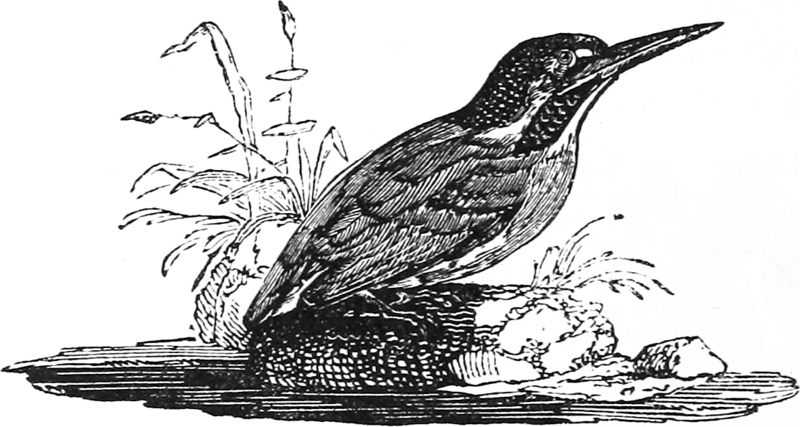
\includegraphics[scale=0.35]{images/Alycon.png}
        \end{figure}
        \vspace{0.5cm}
        \Huge
        \textbf{\textsc{Matematyka Dyskretna}}
        
        \vspace{0.5cm}
        \Large
        \textsc{Wybrane Dowody}
        
        \normalsize
        
        
        \line(1,0){330}
        
        \vspace{1cm}
        \textit{,,Myślę, że 7 punktów na 20 to nie jest zły wynik''}
        \vspace{1cm}

        \textit{\textsc{Popełnione przez}}\\
        \vspace{5mm}

        \textbf{\textsc{Dziurawy Ponton \\ Załatany Ponton \\ Puchaty Pompon \\ Zatopiony Ponton \\ Tonący Ponton \\ Notnop}}

        \vfill

        Kraków \\
        Anno Domini 2023
        
    \end{center}
    
\end{titlepage}


\tableofcontents
\section*{Licencja}
    \begin{figure}[h]
    	\begin{minipage}[c]{0.25\textwidth}
    		
\includegraphics[width=0.7\textwidth]{images/licencja.png}
    	\end{minipage}\hfill
    	\begin{minipage}[c]{0.75\textwidth}
    		\caption*{
    			Ten utwór jest dostępny na 
    			\href{https://creativecommons.org/licenses/by-sa/4.0/}{licencji Creative Commons Uznanie autorstwa
    			na tych samych warunkach 4.0 Międzynarodowe.}
    		}
    	\end{minipage}
    \end{figure}

% Actual content
\mainmatter

\chapter{Kombinatoryka}
 % Żeby nie było syfu to kolejne sekcje dodajemy do chapters/
% A potem includujemy za pomocą \input{chapters/...}

% Używamy \( \) i \[ \] zamiast dolarów -- tak jak się robi w LaTeXu


\documentclass[12pt, a4paper, polish, openany]{book}

% Please, let's familiarize ourselves with notatki.sty and tcs.sty so that we don't reinvent the wheel
\usepackage{notatki}

\fancyhead[L]{\textbf{\textit{MD}}}
\author{
}
\title{TCS and shitposting}


\begin{document}

% Front page and table of contents
\frontmatter

\input{titlepage}

\tableofcontents
\input{license}

% Actual content
\mainmatter

\chapter{Kombinatoryka}
\input{chapters/combinatorics/main}

\chapter{Zasada włączeń i wyłączeń}
\input{chapters/exclusion-inclusion/main}

\chapter{Posety}
\input{chapters/posets/main}

\chapter{Twierdzenie Ramseya}
\input{chapters/ramsey/main}

\chapter{Funkcje tworzące}
\input{chapters/generating_functions/main}

\chapter{Przepływy}
\input{chapters/flows/main}

\chapter{Skojarzenia}
\input{chapters/matchings/main}

\chapter{Kolorowanie grafów}
\input{chapters/graph-coloring/main}

\chapter{Grafy, ale nie kolorowanie}
\input{chapters/graph-misc/main}

\end{document}

\chapter{Zasada włączeń i wyłączeń}
 % Żeby nie było syfu to kolejne sekcje dodajemy do chapters/
% A potem includujemy za pomocą \input{chapters/...}

% Używamy \( \) i \[ \] zamiast dolarów -- tak jak się robi w LaTeXu


\documentclass[12pt, a4paper, polish, openany]{book}

% Please, let's familiarize ourselves with notatki.sty and tcs.sty so that we don't reinvent the wheel
\usepackage{notatki}

\fancyhead[L]{\textbf{\textit{MD}}}
\author{
}
\title{TCS and shitposting}


\begin{document}

% Front page and table of contents
\frontmatter

\input{titlepage}

\tableofcontents
\input{license}

% Actual content
\mainmatter

\chapter{Kombinatoryka}
\input{chapters/combinatorics/main}

\chapter{Zasada włączeń i wyłączeń}
\input{chapters/exclusion-inclusion/main}

\chapter{Posety}
\input{chapters/posets/main}

\chapter{Twierdzenie Ramseya}
\input{chapters/ramsey/main}

\chapter{Funkcje tworzące}
\input{chapters/generating_functions/main}

\chapter{Przepływy}
\input{chapters/flows/main}

\chapter{Skojarzenia}
\input{chapters/matchings/main}

\chapter{Kolorowanie grafów}
\input{chapters/graph-coloring/main}

\chapter{Grafy, ale nie kolorowanie}
\input{chapters/graph-misc/main}

\end{document}

\chapter{Posety}
 % Żeby nie było syfu to kolejne sekcje dodajemy do chapters/
% A potem includujemy za pomocą \input{chapters/...}

% Używamy \( \) i \[ \] zamiast dolarów -- tak jak się robi w LaTeXu


\documentclass[12pt, a4paper, polish, openany]{book}

% Please, let's familiarize ourselves with notatki.sty and tcs.sty so that we don't reinvent the wheel
\usepackage{notatki}

\fancyhead[L]{\textbf{\textit{MD}}}
\author{
}
\title{TCS and shitposting}


\begin{document}

% Front page and table of contents
\frontmatter

\input{titlepage}

\tableofcontents
\input{license}

% Actual content
\mainmatter

\chapter{Kombinatoryka}
\input{chapters/combinatorics/main}

\chapter{Zasada włączeń i wyłączeń}
\input{chapters/exclusion-inclusion/main}

\chapter{Posety}
\input{chapters/posets/main}

\chapter{Twierdzenie Ramseya}
\input{chapters/ramsey/main}

\chapter{Funkcje tworzące}
\input{chapters/generating_functions/main}

\chapter{Przepływy}
\input{chapters/flows/main}

\chapter{Skojarzenia}
\input{chapters/matchings/main}

\chapter{Kolorowanie grafów}
\input{chapters/graph-coloring/main}

\chapter{Grafy, ale nie kolorowanie}
\input{chapters/graph-misc/main}

\end{document}

\chapter{Twierdzenie Ramseya}
 % Żeby nie było syfu to kolejne sekcje dodajemy do chapters/
% A potem includujemy za pomocą \input{chapters/...}

% Używamy \( \) i \[ \] zamiast dolarów -- tak jak się robi w LaTeXu


\documentclass[12pt, a4paper, polish, openany]{book}

% Please, let's familiarize ourselves with notatki.sty and tcs.sty so that we don't reinvent the wheel
\usepackage{notatki}

\fancyhead[L]{\textbf{\textit{MD}}}
\author{
}
\title{TCS and shitposting}


\begin{document}

% Front page and table of contents
\frontmatter

\input{titlepage}

\tableofcontents
\input{license}

% Actual content
\mainmatter

\chapter{Kombinatoryka}
\input{chapters/combinatorics/main}

\chapter{Zasada włączeń i wyłączeń}
\input{chapters/exclusion-inclusion/main}

\chapter{Posety}
\input{chapters/posets/main}

\chapter{Twierdzenie Ramseya}
\input{chapters/ramsey/main}

\chapter{Funkcje tworzące}
\input{chapters/generating_functions/main}

\chapter{Przepływy}
\input{chapters/flows/main}

\chapter{Skojarzenia}
\input{chapters/matchings/main}

\chapter{Kolorowanie grafów}
\input{chapters/graph-coloring/main}

\chapter{Grafy, ale nie kolorowanie}
\input{chapters/graph-misc/main}

\end{document}

\chapter{Funkcje tworzące}
 % Żeby nie było syfu to kolejne sekcje dodajemy do chapters/
% A potem includujemy za pomocą \input{chapters/...}

% Używamy \( \) i \[ \] zamiast dolarów -- tak jak się robi w LaTeXu


\documentclass[12pt, a4paper, polish, openany]{book}

% Please, let's familiarize ourselves with notatki.sty and tcs.sty so that we don't reinvent the wheel
\usepackage{notatki}

\fancyhead[L]{\textbf{\textit{MD}}}
\author{
}
\title{TCS and shitposting}


\begin{document}

% Front page and table of contents
\frontmatter

\input{titlepage}

\tableofcontents
\input{license}

% Actual content
\mainmatter

\chapter{Kombinatoryka}
\input{chapters/combinatorics/main}

\chapter{Zasada włączeń i wyłączeń}
\input{chapters/exclusion-inclusion/main}

\chapter{Posety}
\input{chapters/posets/main}

\chapter{Twierdzenie Ramseya}
\input{chapters/ramsey/main}

\chapter{Funkcje tworzące}
\input{chapters/generating_functions/main}

\chapter{Przepływy}
\input{chapters/flows/main}

\chapter{Skojarzenia}
\input{chapters/matchings/main}

\chapter{Kolorowanie grafów}
\input{chapters/graph-coloring/main}

\chapter{Grafy, ale nie kolorowanie}
\input{chapters/graph-misc/main}

\end{document}

\chapter{Przepływy}
 % Żeby nie było syfu to kolejne sekcje dodajemy do chapters/
% A potem includujemy za pomocą \input{chapters/...}

% Używamy \( \) i \[ \] zamiast dolarów -- tak jak się robi w LaTeXu


\documentclass[12pt, a4paper, polish, openany]{book}

% Please, let's familiarize ourselves with notatki.sty and tcs.sty so that we don't reinvent the wheel
\usepackage{notatki}

\fancyhead[L]{\textbf{\textit{MD}}}
\author{
}
\title{TCS and shitposting}


\begin{document}

% Front page and table of contents
\frontmatter

\input{titlepage}

\tableofcontents
\input{license}

% Actual content
\mainmatter

\chapter{Kombinatoryka}
\input{chapters/combinatorics/main}

\chapter{Zasada włączeń i wyłączeń}
\input{chapters/exclusion-inclusion/main}

\chapter{Posety}
\input{chapters/posets/main}

\chapter{Twierdzenie Ramseya}
\input{chapters/ramsey/main}

\chapter{Funkcje tworzące}
\input{chapters/generating_functions/main}

\chapter{Przepływy}
\input{chapters/flows/main}

\chapter{Skojarzenia}
\input{chapters/matchings/main}

\chapter{Kolorowanie grafów}
\input{chapters/graph-coloring/main}

\chapter{Grafy, ale nie kolorowanie}
\input{chapters/graph-misc/main}

\end{document}

\chapter{Skojarzenia}
 % Żeby nie było syfu to kolejne sekcje dodajemy do chapters/
% A potem includujemy za pomocą \input{chapters/...}

% Używamy \( \) i \[ \] zamiast dolarów -- tak jak się robi w LaTeXu


\documentclass[12pt, a4paper, polish, openany]{book}

% Please, let's familiarize ourselves with notatki.sty and tcs.sty so that we don't reinvent the wheel
\usepackage{notatki}

\fancyhead[L]{\textbf{\textit{MD}}}
\author{
}
\title{TCS and shitposting}


\begin{document}

% Front page and table of contents
\frontmatter

\input{titlepage}

\tableofcontents
\input{license}

% Actual content
\mainmatter

\chapter{Kombinatoryka}
\input{chapters/combinatorics/main}

\chapter{Zasada włączeń i wyłączeń}
\input{chapters/exclusion-inclusion/main}

\chapter{Posety}
\input{chapters/posets/main}

\chapter{Twierdzenie Ramseya}
\input{chapters/ramsey/main}

\chapter{Funkcje tworzące}
\input{chapters/generating_functions/main}

\chapter{Przepływy}
\input{chapters/flows/main}

\chapter{Skojarzenia}
\input{chapters/matchings/main}

\chapter{Kolorowanie grafów}
\input{chapters/graph-coloring/main}

\chapter{Grafy, ale nie kolorowanie}
\input{chapters/graph-misc/main}

\end{document}

\chapter{Kolorowanie grafów}
 % Żeby nie było syfu to kolejne sekcje dodajemy do chapters/
% A potem includujemy za pomocą \input{chapters/...}

% Używamy \( \) i \[ \] zamiast dolarów -- tak jak się robi w LaTeXu


\documentclass[12pt, a4paper, polish, openany]{book}

% Please, let's familiarize ourselves with notatki.sty and tcs.sty so that we don't reinvent the wheel
\usepackage{notatki}

\fancyhead[L]{\textbf{\textit{MD}}}
\author{
}
\title{TCS and shitposting}


\begin{document}

% Front page and table of contents
\frontmatter

\input{titlepage}

\tableofcontents
\input{license}

% Actual content
\mainmatter

\chapter{Kombinatoryka}
\input{chapters/combinatorics/main}

\chapter{Zasada włączeń i wyłączeń}
\input{chapters/exclusion-inclusion/main}

\chapter{Posety}
\input{chapters/posets/main}

\chapter{Twierdzenie Ramseya}
\input{chapters/ramsey/main}

\chapter{Funkcje tworzące}
\input{chapters/generating_functions/main}

\chapter{Przepływy}
\input{chapters/flows/main}

\chapter{Skojarzenia}
\input{chapters/matchings/main}

\chapter{Kolorowanie grafów}
\input{chapters/graph-coloring/main}

\chapter{Grafy, ale nie kolorowanie}
\input{chapters/graph-misc/main}

\end{document}

\chapter{Grafy, ale nie kolorowanie}
 % Żeby nie było syfu to kolejne sekcje dodajemy do chapters/
% A potem includujemy za pomocą \input{chapters/...}

% Używamy \( \) i \[ \] zamiast dolarów -- tak jak się robi w LaTeXu


\documentclass[12pt, a4paper, polish, openany]{book}

% Please, let's familiarize ourselves with notatki.sty and tcs.sty so that we don't reinvent the wheel
\usepackage{notatki}

\fancyhead[L]{\textbf{\textit{MD}}}
\author{
}
\title{TCS and shitposting}


\begin{document}

% Front page and table of contents
\frontmatter

\input{titlepage}

\tableofcontents
\input{license}

% Actual content
\mainmatter

\chapter{Kombinatoryka}
\input{chapters/combinatorics/main}

\chapter{Zasada włączeń i wyłączeń}
\input{chapters/exclusion-inclusion/main}

\chapter{Posety}
\input{chapters/posets/main}

\chapter{Twierdzenie Ramseya}
\input{chapters/ramsey/main}

\chapter{Funkcje tworzące}
\input{chapters/generating_functions/main}

\chapter{Przepływy}
\input{chapters/flows/main}

\chapter{Skojarzenia}
\input{chapters/matchings/main}

\chapter{Kolorowanie grafów}
\input{chapters/graph-coloring/main}

\chapter{Grafy, ale nie kolorowanie}
\input{chapters/graph-misc/main}

\end{document}

\end{document}

\end{document}

\section{Tablice sufiksowe, tworzenie za pomocą algorytmu KMR, definicje funkcji LCP i LCP2, zastosowanie LCP2 do wyszukiwania łańcucha w tekście.}
%  % Żeby nie było syfu to kolejne sekcje dodajemy do chapters/
% A potem includujemy za pomocą \input{chapters/...}

% Używamy \( \) i \[ \] zamiast dolarów -- tak jak się robi w LaTeXu


\documentclass[12pt, a4paper, polish, openany]{book}

% Please, let's familiarize ourselves with notatki.sty and tcs.sty so that we don't reinvent the wheel
\usepackage{notatki}

\fancyhead[L]{\textbf{\textit{MD}}}
\author{
}
\title{TCS and shitposting}


\begin{document}

% Front page and table of contents
\frontmatter

\begin{titlepage} 

    \begin{center}
         \begin{figure}[h]
            \centering
            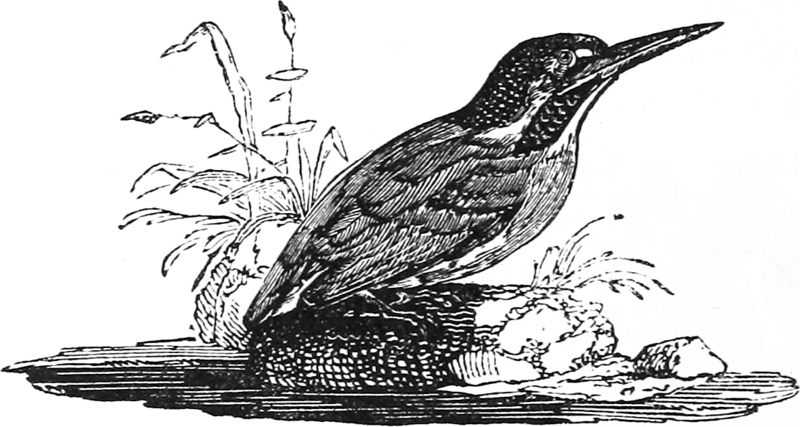
\includegraphics[scale=0.35]{images/Alycon.png}
        \end{figure}
        \vspace{0.5cm}
        \Huge
        \textbf{\textsc{Matematyka Dyskretna}}
        
        \vspace{0.5cm}
        \Large
        \textsc{Wybrane Dowody}
        
        \normalsize
        
        
        \line(1,0){330}
        
        \vspace{1cm}
        \textit{,,Myślę, że 7 punktów na 20 to nie jest zły wynik''}
        \vspace{1cm}

        \textit{\textsc{Popełnione przez}}\\
        \vspace{5mm}

        \textbf{\textsc{Dziurawy Ponton \\ Załatany Ponton \\ Puchaty Pompon \\ Zatopiony Ponton \\ Tonący Ponton \\ Notnop}}

        \vfill

        Kraków \\
        Anno Domini 2023
        
    \end{center}
    
\end{titlepage}


\tableofcontents
\section*{Licencja}
    \begin{figure}[h]
    	\begin{minipage}[c]{0.25\textwidth}
    		
\includegraphics[width=0.7\textwidth]{images/licencja.png}
    	\end{minipage}\hfill
    	\begin{minipage}[c]{0.75\textwidth}
    		\caption*{
    			Ten utwór jest dostępny na 
    			\href{https://creativecommons.org/licenses/by-sa/4.0/}{licencji Creative Commons Uznanie autorstwa
    			na tych samych warunkach 4.0 Międzynarodowe.}
    		}
    	\end{minipage}
    \end{figure}

% Actual content
\mainmatter

\chapter{Kombinatoryka}
 % Żeby nie było syfu to kolejne sekcje dodajemy do chapters/
% A potem includujemy za pomocą \input{chapters/...}

% Używamy \( \) i \[ \] zamiast dolarów -- tak jak się robi w LaTeXu


\documentclass[12pt, a4paper, polish, openany]{book}

% Please, let's familiarize ourselves with notatki.sty and tcs.sty so that we don't reinvent the wheel
\usepackage{notatki}

\fancyhead[L]{\textbf{\textit{MD}}}
\author{
}
\title{TCS and shitposting}


\begin{document}

% Front page and table of contents
\frontmatter

\begin{titlepage} 

    \begin{center}
         \begin{figure}[h]
            \centering
            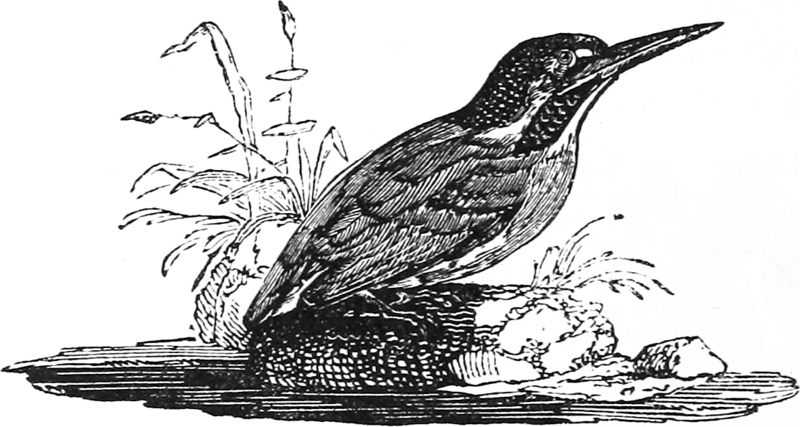
\includegraphics[scale=0.35]{images/Alycon.png}
        \end{figure}
        \vspace{0.5cm}
        \Huge
        \textbf{\textsc{Matematyka Dyskretna}}
        
        \vspace{0.5cm}
        \Large
        \textsc{Wybrane Dowody}
        
        \normalsize
        
        
        \line(1,0){330}
        
        \vspace{1cm}
        \textit{,,Myślę, że 7 punktów na 20 to nie jest zły wynik''}
        \vspace{1cm}

        \textit{\textsc{Popełnione przez}}\\
        \vspace{5mm}

        \textbf{\textsc{Dziurawy Ponton \\ Załatany Ponton \\ Puchaty Pompon \\ Zatopiony Ponton \\ Tonący Ponton \\ Notnop}}

        \vfill

        Kraków \\
        Anno Domini 2023
        
    \end{center}
    
\end{titlepage}


\tableofcontents
\section*{Licencja}
    \begin{figure}[h]
    	\begin{minipage}[c]{0.25\textwidth}
    		
\includegraphics[width=0.7\textwidth]{images/licencja.png}
    	\end{minipage}\hfill
    	\begin{minipage}[c]{0.75\textwidth}
    		\caption*{
    			Ten utwór jest dostępny na 
    			\href{https://creativecommons.org/licenses/by-sa/4.0/}{licencji Creative Commons Uznanie autorstwa
    			na tych samych warunkach 4.0 Międzynarodowe.}
    		}
    	\end{minipage}
    \end{figure}

% Actual content
\mainmatter

\chapter{Kombinatoryka}
 % Żeby nie było syfu to kolejne sekcje dodajemy do chapters/
% A potem includujemy za pomocą \input{chapters/...}

% Używamy \( \) i \[ \] zamiast dolarów -- tak jak się robi w LaTeXu


\documentclass[12pt, a4paper, polish, openany]{book}

% Please, let's familiarize ourselves with notatki.sty and tcs.sty so that we don't reinvent the wheel
\usepackage{notatki}

\fancyhead[L]{\textbf{\textit{MD}}}
\author{
}
\title{TCS and shitposting}


\begin{document}

% Front page and table of contents
\frontmatter

\input{titlepage}

\tableofcontents
\input{license}

% Actual content
\mainmatter

\chapter{Kombinatoryka}
\input{chapters/combinatorics/main}

\chapter{Zasada włączeń i wyłączeń}
\input{chapters/exclusion-inclusion/main}

\chapter{Posety}
\input{chapters/posets/main}

\chapter{Twierdzenie Ramseya}
\input{chapters/ramsey/main}

\chapter{Funkcje tworzące}
\input{chapters/generating_functions/main}

\chapter{Przepływy}
\input{chapters/flows/main}

\chapter{Skojarzenia}
\input{chapters/matchings/main}

\chapter{Kolorowanie grafów}
\input{chapters/graph-coloring/main}

\chapter{Grafy, ale nie kolorowanie}
\input{chapters/graph-misc/main}

\end{document}

\chapter{Zasada włączeń i wyłączeń}
 % Żeby nie było syfu to kolejne sekcje dodajemy do chapters/
% A potem includujemy za pomocą \input{chapters/...}

% Używamy \( \) i \[ \] zamiast dolarów -- tak jak się robi w LaTeXu


\documentclass[12pt, a4paper, polish, openany]{book}

% Please, let's familiarize ourselves with notatki.sty and tcs.sty so that we don't reinvent the wheel
\usepackage{notatki}

\fancyhead[L]{\textbf{\textit{MD}}}
\author{
}
\title{TCS and shitposting}


\begin{document}

% Front page and table of contents
\frontmatter

\input{titlepage}

\tableofcontents
\input{license}

% Actual content
\mainmatter

\chapter{Kombinatoryka}
\input{chapters/combinatorics/main}

\chapter{Zasada włączeń i wyłączeń}
\input{chapters/exclusion-inclusion/main}

\chapter{Posety}
\input{chapters/posets/main}

\chapter{Twierdzenie Ramseya}
\input{chapters/ramsey/main}

\chapter{Funkcje tworzące}
\input{chapters/generating_functions/main}

\chapter{Przepływy}
\input{chapters/flows/main}

\chapter{Skojarzenia}
\input{chapters/matchings/main}

\chapter{Kolorowanie grafów}
\input{chapters/graph-coloring/main}

\chapter{Grafy, ale nie kolorowanie}
\input{chapters/graph-misc/main}

\end{document}

\chapter{Posety}
 % Żeby nie było syfu to kolejne sekcje dodajemy do chapters/
% A potem includujemy za pomocą \input{chapters/...}

% Używamy \( \) i \[ \] zamiast dolarów -- tak jak się robi w LaTeXu


\documentclass[12pt, a4paper, polish, openany]{book}

% Please, let's familiarize ourselves with notatki.sty and tcs.sty so that we don't reinvent the wheel
\usepackage{notatki}

\fancyhead[L]{\textbf{\textit{MD}}}
\author{
}
\title{TCS and shitposting}


\begin{document}

% Front page and table of contents
\frontmatter

\input{titlepage}

\tableofcontents
\input{license}

% Actual content
\mainmatter

\chapter{Kombinatoryka}
\input{chapters/combinatorics/main}

\chapter{Zasada włączeń i wyłączeń}
\input{chapters/exclusion-inclusion/main}

\chapter{Posety}
\input{chapters/posets/main}

\chapter{Twierdzenie Ramseya}
\input{chapters/ramsey/main}

\chapter{Funkcje tworzące}
\input{chapters/generating_functions/main}

\chapter{Przepływy}
\input{chapters/flows/main}

\chapter{Skojarzenia}
\input{chapters/matchings/main}

\chapter{Kolorowanie grafów}
\input{chapters/graph-coloring/main}

\chapter{Grafy, ale nie kolorowanie}
\input{chapters/graph-misc/main}

\end{document}

\chapter{Twierdzenie Ramseya}
 % Żeby nie było syfu to kolejne sekcje dodajemy do chapters/
% A potem includujemy za pomocą \input{chapters/...}

% Używamy \( \) i \[ \] zamiast dolarów -- tak jak się robi w LaTeXu


\documentclass[12pt, a4paper, polish, openany]{book}

% Please, let's familiarize ourselves with notatki.sty and tcs.sty so that we don't reinvent the wheel
\usepackage{notatki}

\fancyhead[L]{\textbf{\textit{MD}}}
\author{
}
\title{TCS and shitposting}


\begin{document}

% Front page and table of contents
\frontmatter

\input{titlepage}

\tableofcontents
\input{license}

% Actual content
\mainmatter

\chapter{Kombinatoryka}
\input{chapters/combinatorics/main}

\chapter{Zasada włączeń i wyłączeń}
\input{chapters/exclusion-inclusion/main}

\chapter{Posety}
\input{chapters/posets/main}

\chapter{Twierdzenie Ramseya}
\input{chapters/ramsey/main}

\chapter{Funkcje tworzące}
\input{chapters/generating_functions/main}

\chapter{Przepływy}
\input{chapters/flows/main}

\chapter{Skojarzenia}
\input{chapters/matchings/main}

\chapter{Kolorowanie grafów}
\input{chapters/graph-coloring/main}

\chapter{Grafy, ale nie kolorowanie}
\input{chapters/graph-misc/main}

\end{document}

\chapter{Funkcje tworzące}
 % Żeby nie było syfu to kolejne sekcje dodajemy do chapters/
% A potem includujemy za pomocą \input{chapters/...}

% Używamy \( \) i \[ \] zamiast dolarów -- tak jak się robi w LaTeXu


\documentclass[12pt, a4paper, polish, openany]{book}

% Please, let's familiarize ourselves with notatki.sty and tcs.sty so that we don't reinvent the wheel
\usepackage{notatki}

\fancyhead[L]{\textbf{\textit{MD}}}
\author{
}
\title{TCS and shitposting}


\begin{document}

% Front page and table of contents
\frontmatter

\input{titlepage}

\tableofcontents
\input{license}

% Actual content
\mainmatter

\chapter{Kombinatoryka}
\input{chapters/combinatorics/main}

\chapter{Zasada włączeń i wyłączeń}
\input{chapters/exclusion-inclusion/main}

\chapter{Posety}
\input{chapters/posets/main}

\chapter{Twierdzenie Ramseya}
\input{chapters/ramsey/main}

\chapter{Funkcje tworzące}
\input{chapters/generating_functions/main}

\chapter{Przepływy}
\input{chapters/flows/main}

\chapter{Skojarzenia}
\input{chapters/matchings/main}

\chapter{Kolorowanie grafów}
\input{chapters/graph-coloring/main}

\chapter{Grafy, ale nie kolorowanie}
\input{chapters/graph-misc/main}

\end{document}

\chapter{Przepływy}
 % Żeby nie było syfu to kolejne sekcje dodajemy do chapters/
% A potem includujemy za pomocą \input{chapters/...}

% Używamy \( \) i \[ \] zamiast dolarów -- tak jak się robi w LaTeXu


\documentclass[12pt, a4paper, polish, openany]{book}

% Please, let's familiarize ourselves with notatki.sty and tcs.sty so that we don't reinvent the wheel
\usepackage{notatki}

\fancyhead[L]{\textbf{\textit{MD}}}
\author{
}
\title{TCS and shitposting}


\begin{document}

% Front page and table of contents
\frontmatter

\input{titlepage}

\tableofcontents
\input{license}

% Actual content
\mainmatter

\chapter{Kombinatoryka}
\input{chapters/combinatorics/main}

\chapter{Zasada włączeń i wyłączeń}
\input{chapters/exclusion-inclusion/main}

\chapter{Posety}
\input{chapters/posets/main}

\chapter{Twierdzenie Ramseya}
\input{chapters/ramsey/main}

\chapter{Funkcje tworzące}
\input{chapters/generating_functions/main}

\chapter{Przepływy}
\input{chapters/flows/main}

\chapter{Skojarzenia}
\input{chapters/matchings/main}

\chapter{Kolorowanie grafów}
\input{chapters/graph-coloring/main}

\chapter{Grafy, ale nie kolorowanie}
\input{chapters/graph-misc/main}

\end{document}

\chapter{Skojarzenia}
 % Żeby nie było syfu to kolejne sekcje dodajemy do chapters/
% A potem includujemy za pomocą \input{chapters/...}

% Używamy \( \) i \[ \] zamiast dolarów -- tak jak się robi w LaTeXu


\documentclass[12pt, a4paper, polish, openany]{book}

% Please, let's familiarize ourselves with notatki.sty and tcs.sty so that we don't reinvent the wheel
\usepackage{notatki}

\fancyhead[L]{\textbf{\textit{MD}}}
\author{
}
\title{TCS and shitposting}


\begin{document}

% Front page and table of contents
\frontmatter

\input{titlepage}

\tableofcontents
\input{license}

% Actual content
\mainmatter

\chapter{Kombinatoryka}
\input{chapters/combinatorics/main}

\chapter{Zasada włączeń i wyłączeń}
\input{chapters/exclusion-inclusion/main}

\chapter{Posety}
\input{chapters/posets/main}

\chapter{Twierdzenie Ramseya}
\input{chapters/ramsey/main}

\chapter{Funkcje tworzące}
\input{chapters/generating_functions/main}

\chapter{Przepływy}
\input{chapters/flows/main}

\chapter{Skojarzenia}
\input{chapters/matchings/main}

\chapter{Kolorowanie grafów}
\input{chapters/graph-coloring/main}

\chapter{Grafy, ale nie kolorowanie}
\input{chapters/graph-misc/main}

\end{document}

\chapter{Kolorowanie grafów}
 % Żeby nie było syfu to kolejne sekcje dodajemy do chapters/
% A potem includujemy za pomocą \input{chapters/...}

% Używamy \( \) i \[ \] zamiast dolarów -- tak jak się robi w LaTeXu


\documentclass[12pt, a4paper, polish, openany]{book}

% Please, let's familiarize ourselves with notatki.sty and tcs.sty so that we don't reinvent the wheel
\usepackage{notatki}

\fancyhead[L]{\textbf{\textit{MD}}}
\author{
}
\title{TCS and shitposting}


\begin{document}

% Front page and table of contents
\frontmatter

\input{titlepage}

\tableofcontents
\input{license}

% Actual content
\mainmatter

\chapter{Kombinatoryka}
\input{chapters/combinatorics/main}

\chapter{Zasada włączeń i wyłączeń}
\input{chapters/exclusion-inclusion/main}

\chapter{Posety}
\input{chapters/posets/main}

\chapter{Twierdzenie Ramseya}
\input{chapters/ramsey/main}

\chapter{Funkcje tworzące}
\input{chapters/generating_functions/main}

\chapter{Przepływy}
\input{chapters/flows/main}

\chapter{Skojarzenia}
\input{chapters/matchings/main}

\chapter{Kolorowanie grafów}
\input{chapters/graph-coloring/main}

\chapter{Grafy, ale nie kolorowanie}
\input{chapters/graph-misc/main}

\end{document}

\chapter{Grafy, ale nie kolorowanie}
 % Żeby nie było syfu to kolejne sekcje dodajemy do chapters/
% A potem includujemy za pomocą \input{chapters/...}

% Używamy \( \) i \[ \] zamiast dolarów -- tak jak się robi w LaTeXu


\documentclass[12pt, a4paper, polish, openany]{book}

% Please, let's familiarize ourselves with notatki.sty and tcs.sty so that we don't reinvent the wheel
\usepackage{notatki}

\fancyhead[L]{\textbf{\textit{MD}}}
\author{
}
\title{TCS and shitposting}


\begin{document}

% Front page and table of contents
\frontmatter

\input{titlepage}

\tableofcontents
\input{license}

% Actual content
\mainmatter

\chapter{Kombinatoryka}
\input{chapters/combinatorics/main}

\chapter{Zasada włączeń i wyłączeń}
\input{chapters/exclusion-inclusion/main}

\chapter{Posety}
\input{chapters/posets/main}

\chapter{Twierdzenie Ramseya}
\input{chapters/ramsey/main}

\chapter{Funkcje tworzące}
\input{chapters/generating_functions/main}

\chapter{Przepływy}
\input{chapters/flows/main}

\chapter{Skojarzenia}
\input{chapters/matchings/main}

\chapter{Kolorowanie grafów}
\input{chapters/graph-coloring/main}

\chapter{Grafy, ale nie kolorowanie}
\input{chapters/graph-misc/main}

\end{document}

\end{document}

\chapter{Zasada włączeń i wyłączeń}
 % Żeby nie było syfu to kolejne sekcje dodajemy do chapters/
% A potem includujemy za pomocą \input{chapters/...}

% Używamy \( \) i \[ \] zamiast dolarów -- tak jak się robi w LaTeXu


\documentclass[12pt, a4paper, polish, openany]{book}

% Please, let's familiarize ourselves with notatki.sty and tcs.sty so that we don't reinvent the wheel
\usepackage{notatki}

\fancyhead[L]{\textbf{\textit{MD}}}
\author{
}
\title{TCS and shitposting}


\begin{document}

% Front page and table of contents
\frontmatter

\begin{titlepage} 

    \begin{center}
         \begin{figure}[h]
            \centering
            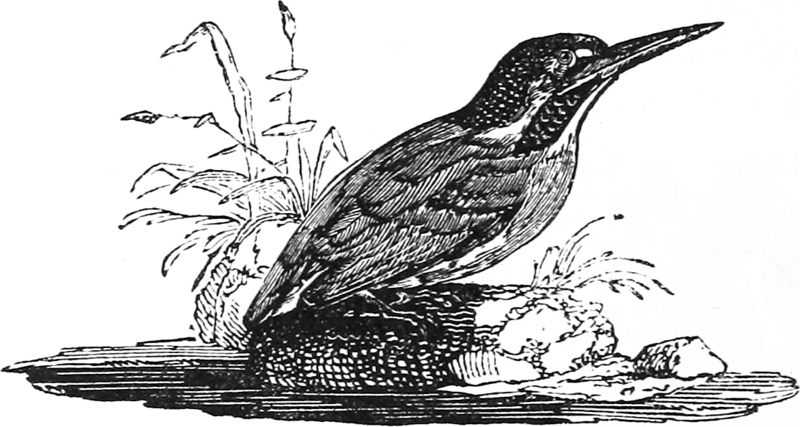
\includegraphics[scale=0.35]{images/Alycon.png}
        \end{figure}
        \vspace{0.5cm}
        \Huge
        \textbf{\textsc{Matematyka Dyskretna}}
        
        \vspace{0.5cm}
        \Large
        \textsc{Wybrane Dowody}
        
        \normalsize
        
        
        \line(1,0){330}
        
        \vspace{1cm}
        \textit{,,Myślę, że 7 punktów na 20 to nie jest zły wynik''}
        \vspace{1cm}

        \textit{\textsc{Popełnione przez}}\\
        \vspace{5mm}

        \textbf{\textsc{Dziurawy Ponton \\ Załatany Ponton \\ Puchaty Pompon \\ Zatopiony Ponton \\ Tonący Ponton \\ Notnop}}

        \vfill

        Kraków \\
        Anno Domini 2023
        
    \end{center}
    
\end{titlepage}


\tableofcontents
\section*{Licencja}
    \begin{figure}[h]
    	\begin{minipage}[c]{0.25\textwidth}
    		
\includegraphics[width=0.7\textwidth]{images/licencja.png}
    	\end{minipage}\hfill
    	\begin{minipage}[c]{0.75\textwidth}
    		\caption*{
    			Ten utwór jest dostępny na 
    			\href{https://creativecommons.org/licenses/by-sa/4.0/}{licencji Creative Commons Uznanie autorstwa
    			na tych samych warunkach 4.0 Międzynarodowe.}
    		}
    	\end{minipage}
    \end{figure}

% Actual content
\mainmatter

\chapter{Kombinatoryka}
 % Żeby nie było syfu to kolejne sekcje dodajemy do chapters/
% A potem includujemy za pomocą \input{chapters/...}

% Używamy \( \) i \[ \] zamiast dolarów -- tak jak się robi w LaTeXu


\documentclass[12pt, a4paper, polish, openany]{book}

% Please, let's familiarize ourselves with notatki.sty and tcs.sty so that we don't reinvent the wheel
\usepackage{notatki}

\fancyhead[L]{\textbf{\textit{MD}}}
\author{
}
\title{TCS and shitposting}


\begin{document}

% Front page and table of contents
\frontmatter

\input{titlepage}

\tableofcontents
\input{license}

% Actual content
\mainmatter

\chapter{Kombinatoryka}
\input{chapters/combinatorics/main}

\chapter{Zasada włączeń i wyłączeń}
\input{chapters/exclusion-inclusion/main}

\chapter{Posety}
\input{chapters/posets/main}

\chapter{Twierdzenie Ramseya}
\input{chapters/ramsey/main}

\chapter{Funkcje tworzące}
\input{chapters/generating_functions/main}

\chapter{Przepływy}
\input{chapters/flows/main}

\chapter{Skojarzenia}
\input{chapters/matchings/main}

\chapter{Kolorowanie grafów}
\input{chapters/graph-coloring/main}

\chapter{Grafy, ale nie kolorowanie}
\input{chapters/graph-misc/main}

\end{document}

\chapter{Zasada włączeń i wyłączeń}
 % Żeby nie było syfu to kolejne sekcje dodajemy do chapters/
% A potem includujemy za pomocą \input{chapters/...}

% Używamy \( \) i \[ \] zamiast dolarów -- tak jak się robi w LaTeXu


\documentclass[12pt, a4paper, polish, openany]{book}

% Please, let's familiarize ourselves with notatki.sty and tcs.sty so that we don't reinvent the wheel
\usepackage{notatki}

\fancyhead[L]{\textbf{\textit{MD}}}
\author{
}
\title{TCS and shitposting}


\begin{document}

% Front page and table of contents
\frontmatter

\input{titlepage}

\tableofcontents
\input{license}

% Actual content
\mainmatter

\chapter{Kombinatoryka}
\input{chapters/combinatorics/main}

\chapter{Zasada włączeń i wyłączeń}
\input{chapters/exclusion-inclusion/main}

\chapter{Posety}
\input{chapters/posets/main}

\chapter{Twierdzenie Ramseya}
\input{chapters/ramsey/main}

\chapter{Funkcje tworzące}
\input{chapters/generating_functions/main}

\chapter{Przepływy}
\input{chapters/flows/main}

\chapter{Skojarzenia}
\input{chapters/matchings/main}

\chapter{Kolorowanie grafów}
\input{chapters/graph-coloring/main}

\chapter{Grafy, ale nie kolorowanie}
\input{chapters/graph-misc/main}

\end{document}

\chapter{Posety}
 % Żeby nie było syfu to kolejne sekcje dodajemy do chapters/
% A potem includujemy za pomocą \input{chapters/...}

% Używamy \( \) i \[ \] zamiast dolarów -- tak jak się robi w LaTeXu


\documentclass[12pt, a4paper, polish, openany]{book}

% Please, let's familiarize ourselves with notatki.sty and tcs.sty so that we don't reinvent the wheel
\usepackage{notatki}

\fancyhead[L]{\textbf{\textit{MD}}}
\author{
}
\title{TCS and shitposting}


\begin{document}

% Front page and table of contents
\frontmatter

\input{titlepage}

\tableofcontents
\input{license}

% Actual content
\mainmatter

\chapter{Kombinatoryka}
\input{chapters/combinatorics/main}

\chapter{Zasada włączeń i wyłączeń}
\input{chapters/exclusion-inclusion/main}

\chapter{Posety}
\input{chapters/posets/main}

\chapter{Twierdzenie Ramseya}
\input{chapters/ramsey/main}

\chapter{Funkcje tworzące}
\input{chapters/generating_functions/main}

\chapter{Przepływy}
\input{chapters/flows/main}

\chapter{Skojarzenia}
\input{chapters/matchings/main}

\chapter{Kolorowanie grafów}
\input{chapters/graph-coloring/main}

\chapter{Grafy, ale nie kolorowanie}
\input{chapters/graph-misc/main}

\end{document}

\chapter{Twierdzenie Ramseya}
 % Żeby nie było syfu to kolejne sekcje dodajemy do chapters/
% A potem includujemy za pomocą \input{chapters/...}

% Używamy \( \) i \[ \] zamiast dolarów -- tak jak się robi w LaTeXu


\documentclass[12pt, a4paper, polish, openany]{book}

% Please, let's familiarize ourselves with notatki.sty and tcs.sty so that we don't reinvent the wheel
\usepackage{notatki}

\fancyhead[L]{\textbf{\textit{MD}}}
\author{
}
\title{TCS and shitposting}


\begin{document}

% Front page and table of contents
\frontmatter

\input{titlepage}

\tableofcontents
\input{license}

% Actual content
\mainmatter

\chapter{Kombinatoryka}
\input{chapters/combinatorics/main}

\chapter{Zasada włączeń i wyłączeń}
\input{chapters/exclusion-inclusion/main}

\chapter{Posety}
\input{chapters/posets/main}

\chapter{Twierdzenie Ramseya}
\input{chapters/ramsey/main}

\chapter{Funkcje tworzące}
\input{chapters/generating_functions/main}

\chapter{Przepływy}
\input{chapters/flows/main}

\chapter{Skojarzenia}
\input{chapters/matchings/main}

\chapter{Kolorowanie grafów}
\input{chapters/graph-coloring/main}

\chapter{Grafy, ale nie kolorowanie}
\input{chapters/graph-misc/main}

\end{document}

\chapter{Funkcje tworzące}
 % Żeby nie było syfu to kolejne sekcje dodajemy do chapters/
% A potem includujemy za pomocą \input{chapters/...}

% Używamy \( \) i \[ \] zamiast dolarów -- tak jak się robi w LaTeXu


\documentclass[12pt, a4paper, polish, openany]{book}

% Please, let's familiarize ourselves with notatki.sty and tcs.sty so that we don't reinvent the wheel
\usepackage{notatki}

\fancyhead[L]{\textbf{\textit{MD}}}
\author{
}
\title{TCS and shitposting}


\begin{document}

% Front page and table of contents
\frontmatter

\input{titlepage}

\tableofcontents
\input{license}

% Actual content
\mainmatter

\chapter{Kombinatoryka}
\input{chapters/combinatorics/main}

\chapter{Zasada włączeń i wyłączeń}
\input{chapters/exclusion-inclusion/main}

\chapter{Posety}
\input{chapters/posets/main}

\chapter{Twierdzenie Ramseya}
\input{chapters/ramsey/main}

\chapter{Funkcje tworzące}
\input{chapters/generating_functions/main}

\chapter{Przepływy}
\input{chapters/flows/main}

\chapter{Skojarzenia}
\input{chapters/matchings/main}

\chapter{Kolorowanie grafów}
\input{chapters/graph-coloring/main}

\chapter{Grafy, ale nie kolorowanie}
\input{chapters/graph-misc/main}

\end{document}

\chapter{Przepływy}
 % Żeby nie było syfu to kolejne sekcje dodajemy do chapters/
% A potem includujemy za pomocą \input{chapters/...}

% Używamy \( \) i \[ \] zamiast dolarów -- tak jak się robi w LaTeXu


\documentclass[12pt, a4paper, polish, openany]{book}

% Please, let's familiarize ourselves with notatki.sty and tcs.sty so that we don't reinvent the wheel
\usepackage{notatki}

\fancyhead[L]{\textbf{\textit{MD}}}
\author{
}
\title{TCS and shitposting}


\begin{document}

% Front page and table of contents
\frontmatter

\input{titlepage}

\tableofcontents
\input{license}

% Actual content
\mainmatter

\chapter{Kombinatoryka}
\input{chapters/combinatorics/main}

\chapter{Zasada włączeń i wyłączeń}
\input{chapters/exclusion-inclusion/main}

\chapter{Posety}
\input{chapters/posets/main}

\chapter{Twierdzenie Ramseya}
\input{chapters/ramsey/main}

\chapter{Funkcje tworzące}
\input{chapters/generating_functions/main}

\chapter{Przepływy}
\input{chapters/flows/main}

\chapter{Skojarzenia}
\input{chapters/matchings/main}

\chapter{Kolorowanie grafów}
\input{chapters/graph-coloring/main}

\chapter{Grafy, ale nie kolorowanie}
\input{chapters/graph-misc/main}

\end{document}

\chapter{Skojarzenia}
 % Żeby nie było syfu to kolejne sekcje dodajemy do chapters/
% A potem includujemy za pomocą \input{chapters/...}

% Używamy \( \) i \[ \] zamiast dolarów -- tak jak się robi w LaTeXu


\documentclass[12pt, a4paper, polish, openany]{book}

% Please, let's familiarize ourselves with notatki.sty and tcs.sty so that we don't reinvent the wheel
\usepackage{notatki}

\fancyhead[L]{\textbf{\textit{MD}}}
\author{
}
\title{TCS and shitposting}


\begin{document}

% Front page and table of contents
\frontmatter

\input{titlepage}

\tableofcontents
\input{license}

% Actual content
\mainmatter

\chapter{Kombinatoryka}
\input{chapters/combinatorics/main}

\chapter{Zasada włączeń i wyłączeń}
\input{chapters/exclusion-inclusion/main}

\chapter{Posety}
\input{chapters/posets/main}

\chapter{Twierdzenie Ramseya}
\input{chapters/ramsey/main}

\chapter{Funkcje tworzące}
\input{chapters/generating_functions/main}

\chapter{Przepływy}
\input{chapters/flows/main}

\chapter{Skojarzenia}
\input{chapters/matchings/main}

\chapter{Kolorowanie grafów}
\input{chapters/graph-coloring/main}

\chapter{Grafy, ale nie kolorowanie}
\input{chapters/graph-misc/main}

\end{document}

\chapter{Kolorowanie grafów}
 % Żeby nie było syfu to kolejne sekcje dodajemy do chapters/
% A potem includujemy za pomocą \input{chapters/...}

% Używamy \( \) i \[ \] zamiast dolarów -- tak jak się robi w LaTeXu


\documentclass[12pt, a4paper, polish, openany]{book}

% Please, let's familiarize ourselves with notatki.sty and tcs.sty so that we don't reinvent the wheel
\usepackage{notatki}

\fancyhead[L]{\textbf{\textit{MD}}}
\author{
}
\title{TCS and shitposting}


\begin{document}

% Front page and table of contents
\frontmatter

\input{titlepage}

\tableofcontents
\input{license}

% Actual content
\mainmatter

\chapter{Kombinatoryka}
\input{chapters/combinatorics/main}

\chapter{Zasada włączeń i wyłączeń}
\input{chapters/exclusion-inclusion/main}

\chapter{Posety}
\input{chapters/posets/main}

\chapter{Twierdzenie Ramseya}
\input{chapters/ramsey/main}

\chapter{Funkcje tworzące}
\input{chapters/generating_functions/main}

\chapter{Przepływy}
\input{chapters/flows/main}

\chapter{Skojarzenia}
\input{chapters/matchings/main}

\chapter{Kolorowanie grafów}
\input{chapters/graph-coloring/main}

\chapter{Grafy, ale nie kolorowanie}
\input{chapters/graph-misc/main}

\end{document}

\chapter{Grafy, ale nie kolorowanie}
 % Żeby nie było syfu to kolejne sekcje dodajemy do chapters/
% A potem includujemy za pomocą \input{chapters/...}

% Używamy \( \) i \[ \] zamiast dolarów -- tak jak się robi w LaTeXu


\documentclass[12pt, a4paper, polish, openany]{book}

% Please, let's familiarize ourselves with notatki.sty and tcs.sty so that we don't reinvent the wheel
\usepackage{notatki}

\fancyhead[L]{\textbf{\textit{MD}}}
\author{
}
\title{TCS and shitposting}


\begin{document}

% Front page and table of contents
\frontmatter

\input{titlepage}

\tableofcontents
\input{license}

% Actual content
\mainmatter

\chapter{Kombinatoryka}
\input{chapters/combinatorics/main}

\chapter{Zasada włączeń i wyłączeń}
\input{chapters/exclusion-inclusion/main}

\chapter{Posety}
\input{chapters/posets/main}

\chapter{Twierdzenie Ramseya}
\input{chapters/ramsey/main}

\chapter{Funkcje tworzące}
\input{chapters/generating_functions/main}

\chapter{Przepływy}
\input{chapters/flows/main}

\chapter{Skojarzenia}
\input{chapters/matchings/main}

\chapter{Kolorowanie grafów}
\input{chapters/graph-coloring/main}

\chapter{Grafy, ale nie kolorowanie}
\input{chapters/graph-misc/main}

\end{document}

\end{document}

\chapter{Posety}
 % Żeby nie było syfu to kolejne sekcje dodajemy do chapters/
% A potem includujemy za pomocą \input{chapters/...}

% Używamy \( \) i \[ \] zamiast dolarów -- tak jak się robi w LaTeXu


\documentclass[12pt, a4paper, polish, openany]{book}

% Please, let's familiarize ourselves with notatki.sty and tcs.sty so that we don't reinvent the wheel
\usepackage{notatki}

\fancyhead[L]{\textbf{\textit{MD}}}
\author{
}
\title{TCS and shitposting}


\begin{document}

% Front page and table of contents
\frontmatter

\begin{titlepage} 

    \begin{center}
         \begin{figure}[h]
            \centering
            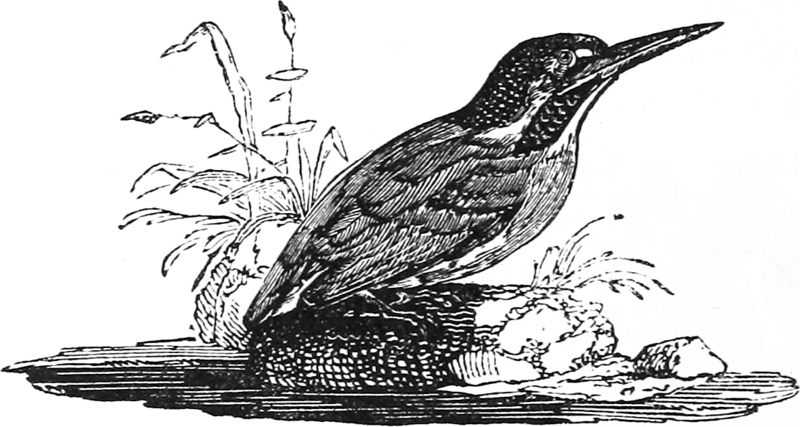
\includegraphics[scale=0.35]{images/Alycon.png}
        \end{figure}
        \vspace{0.5cm}
        \Huge
        \textbf{\textsc{Matematyka Dyskretna}}
        
        \vspace{0.5cm}
        \Large
        \textsc{Wybrane Dowody}
        
        \normalsize
        
        
        \line(1,0){330}
        
        \vspace{1cm}
        \textit{,,Myślę, że 7 punktów na 20 to nie jest zły wynik''}
        \vspace{1cm}

        \textit{\textsc{Popełnione przez}}\\
        \vspace{5mm}

        \textbf{\textsc{Dziurawy Ponton \\ Załatany Ponton \\ Puchaty Pompon \\ Zatopiony Ponton \\ Tonący Ponton \\ Notnop}}

        \vfill

        Kraków \\
        Anno Domini 2023
        
    \end{center}
    
\end{titlepage}


\tableofcontents
\section*{Licencja}
    \begin{figure}[h]
    	\begin{minipage}[c]{0.25\textwidth}
    		
\includegraphics[width=0.7\textwidth]{images/licencja.png}
    	\end{minipage}\hfill
    	\begin{minipage}[c]{0.75\textwidth}
    		\caption*{
    			Ten utwór jest dostępny na 
    			\href{https://creativecommons.org/licenses/by-sa/4.0/}{licencji Creative Commons Uznanie autorstwa
    			na tych samych warunkach 4.0 Międzynarodowe.}
    		}
    	\end{minipage}
    \end{figure}

% Actual content
\mainmatter

\chapter{Kombinatoryka}
 % Żeby nie było syfu to kolejne sekcje dodajemy do chapters/
% A potem includujemy za pomocą \input{chapters/...}

% Używamy \( \) i \[ \] zamiast dolarów -- tak jak się robi w LaTeXu


\documentclass[12pt, a4paper, polish, openany]{book}

% Please, let's familiarize ourselves with notatki.sty and tcs.sty so that we don't reinvent the wheel
\usepackage{notatki}

\fancyhead[L]{\textbf{\textit{MD}}}
\author{
}
\title{TCS and shitposting}


\begin{document}

% Front page and table of contents
\frontmatter

\input{titlepage}

\tableofcontents
\input{license}

% Actual content
\mainmatter

\chapter{Kombinatoryka}
\input{chapters/combinatorics/main}

\chapter{Zasada włączeń i wyłączeń}
\input{chapters/exclusion-inclusion/main}

\chapter{Posety}
\input{chapters/posets/main}

\chapter{Twierdzenie Ramseya}
\input{chapters/ramsey/main}

\chapter{Funkcje tworzące}
\input{chapters/generating_functions/main}

\chapter{Przepływy}
\input{chapters/flows/main}

\chapter{Skojarzenia}
\input{chapters/matchings/main}

\chapter{Kolorowanie grafów}
\input{chapters/graph-coloring/main}

\chapter{Grafy, ale nie kolorowanie}
\input{chapters/graph-misc/main}

\end{document}

\chapter{Zasada włączeń i wyłączeń}
 % Żeby nie było syfu to kolejne sekcje dodajemy do chapters/
% A potem includujemy za pomocą \input{chapters/...}

% Używamy \( \) i \[ \] zamiast dolarów -- tak jak się robi w LaTeXu


\documentclass[12pt, a4paper, polish, openany]{book}

% Please, let's familiarize ourselves with notatki.sty and tcs.sty so that we don't reinvent the wheel
\usepackage{notatki}

\fancyhead[L]{\textbf{\textit{MD}}}
\author{
}
\title{TCS and shitposting}


\begin{document}

% Front page and table of contents
\frontmatter

\input{titlepage}

\tableofcontents
\input{license}

% Actual content
\mainmatter

\chapter{Kombinatoryka}
\input{chapters/combinatorics/main}

\chapter{Zasada włączeń i wyłączeń}
\input{chapters/exclusion-inclusion/main}

\chapter{Posety}
\input{chapters/posets/main}

\chapter{Twierdzenie Ramseya}
\input{chapters/ramsey/main}

\chapter{Funkcje tworzące}
\input{chapters/generating_functions/main}

\chapter{Przepływy}
\input{chapters/flows/main}

\chapter{Skojarzenia}
\input{chapters/matchings/main}

\chapter{Kolorowanie grafów}
\input{chapters/graph-coloring/main}

\chapter{Grafy, ale nie kolorowanie}
\input{chapters/graph-misc/main}

\end{document}

\chapter{Posety}
 % Żeby nie było syfu to kolejne sekcje dodajemy do chapters/
% A potem includujemy za pomocą \input{chapters/...}

% Używamy \( \) i \[ \] zamiast dolarów -- tak jak się robi w LaTeXu


\documentclass[12pt, a4paper, polish, openany]{book}

% Please, let's familiarize ourselves with notatki.sty and tcs.sty so that we don't reinvent the wheel
\usepackage{notatki}

\fancyhead[L]{\textbf{\textit{MD}}}
\author{
}
\title{TCS and shitposting}


\begin{document}

% Front page and table of contents
\frontmatter

\input{titlepage}

\tableofcontents
\input{license}

% Actual content
\mainmatter

\chapter{Kombinatoryka}
\input{chapters/combinatorics/main}

\chapter{Zasada włączeń i wyłączeń}
\input{chapters/exclusion-inclusion/main}

\chapter{Posety}
\input{chapters/posets/main}

\chapter{Twierdzenie Ramseya}
\input{chapters/ramsey/main}

\chapter{Funkcje tworzące}
\input{chapters/generating_functions/main}

\chapter{Przepływy}
\input{chapters/flows/main}

\chapter{Skojarzenia}
\input{chapters/matchings/main}

\chapter{Kolorowanie grafów}
\input{chapters/graph-coloring/main}

\chapter{Grafy, ale nie kolorowanie}
\input{chapters/graph-misc/main}

\end{document}

\chapter{Twierdzenie Ramseya}
 % Żeby nie było syfu to kolejne sekcje dodajemy do chapters/
% A potem includujemy za pomocą \input{chapters/...}

% Używamy \( \) i \[ \] zamiast dolarów -- tak jak się robi w LaTeXu


\documentclass[12pt, a4paper, polish, openany]{book}

% Please, let's familiarize ourselves with notatki.sty and tcs.sty so that we don't reinvent the wheel
\usepackage{notatki}

\fancyhead[L]{\textbf{\textit{MD}}}
\author{
}
\title{TCS and shitposting}


\begin{document}

% Front page and table of contents
\frontmatter

\input{titlepage}

\tableofcontents
\input{license}

% Actual content
\mainmatter

\chapter{Kombinatoryka}
\input{chapters/combinatorics/main}

\chapter{Zasada włączeń i wyłączeń}
\input{chapters/exclusion-inclusion/main}

\chapter{Posety}
\input{chapters/posets/main}

\chapter{Twierdzenie Ramseya}
\input{chapters/ramsey/main}

\chapter{Funkcje tworzące}
\input{chapters/generating_functions/main}

\chapter{Przepływy}
\input{chapters/flows/main}

\chapter{Skojarzenia}
\input{chapters/matchings/main}

\chapter{Kolorowanie grafów}
\input{chapters/graph-coloring/main}

\chapter{Grafy, ale nie kolorowanie}
\input{chapters/graph-misc/main}

\end{document}

\chapter{Funkcje tworzące}
 % Żeby nie było syfu to kolejne sekcje dodajemy do chapters/
% A potem includujemy za pomocą \input{chapters/...}

% Używamy \( \) i \[ \] zamiast dolarów -- tak jak się robi w LaTeXu


\documentclass[12pt, a4paper, polish, openany]{book}

% Please, let's familiarize ourselves with notatki.sty and tcs.sty so that we don't reinvent the wheel
\usepackage{notatki}

\fancyhead[L]{\textbf{\textit{MD}}}
\author{
}
\title{TCS and shitposting}


\begin{document}

% Front page and table of contents
\frontmatter

\input{titlepage}

\tableofcontents
\input{license}

% Actual content
\mainmatter

\chapter{Kombinatoryka}
\input{chapters/combinatorics/main}

\chapter{Zasada włączeń i wyłączeń}
\input{chapters/exclusion-inclusion/main}

\chapter{Posety}
\input{chapters/posets/main}

\chapter{Twierdzenie Ramseya}
\input{chapters/ramsey/main}

\chapter{Funkcje tworzące}
\input{chapters/generating_functions/main}

\chapter{Przepływy}
\input{chapters/flows/main}

\chapter{Skojarzenia}
\input{chapters/matchings/main}

\chapter{Kolorowanie grafów}
\input{chapters/graph-coloring/main}

\chapter{Grafy, ale nie kolorowanie}
\input{chapters/graph-misc/main}

\end{document}

\chapter{Przepływy}
 % Żeby nie było syfu to kolejne sekcje dodajemy do chapters/
% A potem includujemy za pomocą \input{chapters/...}

% Używamy \( \) i \[ \] zamiast dolarów -- tak jak się robi w LaTeXu


\documentclass[12pt, a4paper, polish, openany]{book}

% Please, let's familiarize ourselves with notatki.sty and tcs.sty so that we don't reinvent the wheel
\usepackage{notatki}

\fancyhead[L]{\textbf{\textit{MD}}}
\author{
}
\title{TCS and shitposting}


\begin{document}

% Front page and table of contents
\frontmatter

\input{titlepage}

\tableofcontents
\input{license}

% Actual content
\mainmatter

\chapter{Kombinatoryka}
\input{chapters/combinatorics/main}

\chapter{Zasada włączeń i wyłączeń}
\input{chapters/exclusion-inclusion/main}

\chapter{Posety}
\input{chapters/posets/main}

\chapter{Twierdzenie Ramseya}
\input{chapters/ramsey/main}

\chapter{Funkcje tworzące}
\input{chapters/generating_functions/main}

\chapter{Przepływy}
\input{chapters/flows/main}

\chapter{Skojarzenia}
\input{chapters/matchings/main}

\chapter{Kolorowanie grafów}
\input{chapters/graph-coloring/main}

\chapter{Grafy, ale nie kolorowanie}
\input{chapters/graph-misc/main}

\end{document}

\chapter{Skojarzenia}
 % Żeby nie było syfu to kolejne sekcje dodajemy do chapters/
% A potem includujemy za pomocą \input{chapters/...}

% Używamy \( \) i \[ \] zamiast dolarów -- tak jak się robi w LaTeXu


\documentclass[12pt, a4paper, polish, openany]{book}

% Please, let's familiarize ourselves with notatki.sty and tcs.sty so that we don't reinvent the wheel
\usepackage{notatki}

\fancyhead[L]{\textbf{\textit{MD}}}
\author{
}
\title{TCS and shitposting}


\begin{document}

% Front page and table of contents
\frontmatter

\input{titlepage}

\tableofcontents
\input{license}

% Actual content
\mainmatter

\chapter{Kombinatoryka}
\input{chapters/combinatorics/main}

\chapter{Zasada włączeń i wyłączeń}
\input{chapters/exclusion-inclusion/main}

\chapter{Posety}
\input{chapters/posets/main}

\chapter{Twierdzenie Ramseya}
\input{chapters/ramsey/main}

\chapter{Funkcje tworzące}
\input{chapters/generating_functions/main}

\chapter{Przepływy}
\input{chapters/flows/main}

\chapter{Skojarzenia}
\input{chapters/matchings/main}

\chapter{Kolorowanie grafów}
\input{chapters/graph-coloring/main}

\chapter{Grafy, ale nie kolorowanie}
\input{chapters/graph-misc/main}

\end{document}

\chapter{Kolorowanie grafów}
 % Żeby nie było syfu to kolejne sekcje dodajemy do chapters/
% A potem includujemy za pomocą \input{chapters/...}

% Używamy \( \) i \[ \] zamiast dolarów -- tak jak się robi w LaTeXu


\documentclass[12pt, a4paper, polish, openany]{book}

% Please, let's familiarize ourselves with notatki.sty and tcs.sty so that we don't reinvent the wheel
\usepackage{notatki}

\fancyhead[L]{\textbf{\textit{MD}}}
\author{
}
\title{TCS and shitposting}


\begin{document}

% Front page and table of contents
\frontmatter

\input{titlepage}

\tableofcontents
\input{license}

% Actual content
\mainmatter

\chapter{Kombinatoryka}
\input{chapters/combinatorics/main}

\chapter{Zasada włączeń i wyłączeń}
\input{chapters/exclusion-inclusion/main}

\chapter{Posety}
\input{chapters/posets/main}

\chapter{Twierdzenie Ramseya}
\input{chapters/ramsey/main}

\chapter{Funkcje tworzące}
\input{chapters/generating_functions/main}

\chapter{Przepływy}
\input{chapters/flows/main}

\chapter{Skojarzenia}
\input{chapters/matchings/main}

\chapter{Kolorowanie grafów}
\input{chapters/graph-coloring/main}

\chapter{Grafy, ale nie kolorowanie}
\input{chapters/graph-misc/main}

\end{document}

\chapter{Grafy, ale nie kolorowanie}
 % Żeby nie było syfu to kolejne sekcje dodajemy do chapters/
% A potem includujemy za pomocą \input{chapters/...}

% Używamy \( \) i \[ \] zamiast dolarów -- tak jak się robi w LaTeXu


\documentclass[12pt, a4paper, polish, openany]{book}

% Please, let's familiarize ourselves with notatki.sty and tcs.sty so that we don't reinvent the wheel
\usepackage{notatki}

\fancyhead[L]{\textbf{\textit{MD}}}
\author{
}
\title{TCS and shitposting}


\begin{document}

% Front page and table of contents
\frontmatter

\input{titlepage}

\tableofcontents
\input{license}

% Actual content
\mainmatter

\chapter{Kombinatoryka}
\input{chapters/combinatorics/main}

\chapter{Zasada włączeń i wyłączeń}
\input{chapters/exclusion-inclusion/main}

\chapter{Posety}
\input{chapters/posets/main}

\chapter{Twierdzenie Ramseya}
\input{chapters/ramsey/main}

\chapter{Funkcje tworzące}
\input{chapters/generating_functions/main}

\chapter{Przepływy}
\input{chapters/flows/main}

\chapter{Skojarzenia}
\input{chapters/matchings/main}

\chapter{Kolorowanie grafów}
\input{chapters/graph-coloring/main}

\chapter{Grafy, ale nie kolorowanie}
\input{chapters/graph-misc/main}

\end{document}

\end{document}

\chapter{Twierdzenie Ramseya}
 % Żeby nie było syfu to kolejne sekcje dodajemy do chapters/
% A potem includujemy za pomocą \input{chapters/...}

% Używamy \( \) i \[ \] zamiast dolarów -- tak jak się robi w LaTeXu


\documentclass[12pt, a4paper, polish, openany]{book}

% Please, let's familiarize ourselves with notatki.sty and tcs.sty so that we don't reinvent the wheel
\usepackage{notatki}

\fancyhead[L]{\textbf{\textit{MD}}}
\author{
}
\title{TCS and shitposting}


\begin{document}

% Front page and table of contents
\frontmatter

\begin{titlepage} 

    \begin{center}
         \begin{figure}[h]
            \centering
            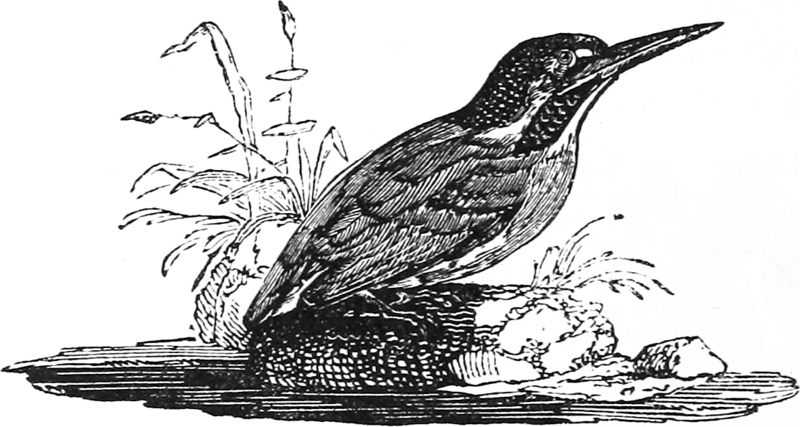
\includegraphics[scale=0.35]{images/Alycon.png}
        \end{figure}
        \vspace{0.5cm}
        \Huge
        \textbf{\textsc{Matematyka Dyskretna}}
        
        \vspace{0.5cm}
        \Large
        \textsc{Wybrane Dowody}
        
        \normalsize
        
        
        \line(1,0){330}
        
        \vspace{1cm}
        \textit{,,Myślę, że 7 punktów na 20 to nie jest zły wynik''}
        \vspace{1cm}

        \textit{\textsc{Popełnione przez}}\\
        \vspace{5mm}

        \textbf{\textsc{Dziurawy Ponton \\ Załatany Ponton \\ Puchaty Pompon \\ Zatopiony Ponton \\ Tonący Ponton \\ Notnop}}

        \vfill

        Kraków \\
        Anno Domini 2023
        
    \end{center}
    
\end{titlepage}


\tableofcontents
\section*{Licencja}
    \begin{figure}[h]
    	\begin{minipage}[c]{0.25\textwidth}
    		
\includegraphics[width=0.7\textwidth]{images/licencja.png}
    	\end{minipage}\hfill
    	\begin{minipage}[c]{0.75\textwidth}
    		\caption*{
    			Ten utwór jest dostępny na 
    			\href{https://creativecommons.org/licenses/by-sa/4.0/}{licencji Creative Commons Uznanie autorstwa
    			na tych samych warunkach 4.0 Międzynarodowe.}
    		}
    	\end{minipage}
    \end{figure}

% Actual content
\mainmatter

\chapter{Kombinatoryka}
 % Żeby nie było syfu to kolejne sekcje dodajemy do chapters/
% A potem includujemy za pomocą \input{chapters/...}

% Używamy \( \) i \[ \] zamiast dolarów -- tak jak się robi w LaTeXu


\documentclass[12pt, a4paper, polish, openany]{book}

% Please, let's familiarize ourselves with notatki.sty and tcs.sty so that we don't reinvent the wheel
\usepackage{notatki}

\fancyhead[L]{\textbf{\textit{MD}}}
\author{
}
\title{TCS and shitposting}


\begin{document}

% Front page and table of contents
\frontmatter

\input{titlepage}

\tableofcontents
\input{license}

% Actual content
\mainmatter

\chapter{Kombinatoryka}
\input{chapters/combinatorics/main}

\chapter{Zasada włączeń i wyłączeń}
\input{chapters/exclusion-inclusion/main}

\chapter{Posety}
\input{chapters/posets/main}

\chapter{Twierdzenie Ramseya}
\input{chapters/ramsey/main}

\chapter{Funkcje tworzące}
\input{chapters/generating_functions/main}

\chapter{Przepływy}
\input{chapters/flows/main}

\chapter{Skojarzenia}
\input{chapters/matchings/main}

\chapter{Kolorowanie grafów}
\input{chapters/graph-coloring/main}

\chapter{Grafy, ale nie kolorowanie}
\input{chapters/graph-misc/main}

\end{document}

\chapter{Zasada włączeń i wyłączeń}
 % Żeby nie było syfu to kolejne sekcje dodajemy do chapters/
% A potem includujemy za pomocą \input{chapters/...}

% Używamy \( \) i \[ \] zamiast dolarów -- tak jak się robi w LaTeXu


\documentclass[12pt, a4paper, polish, openany]{book}

% Please, let's familiarize ourselves with notatki.sty and tcs.sty so that we don't reinvent the wheel
\usepackage{notatki}

\fancyhead[L]{\textbf{\textit{MD}}}
\author{
}
\title{TCS and shitposting}


\begin{document}

% Front page and table of contents
\frontmatter

\input{titlepage}

\tableofcontents
\input{license}

% Actual content
\mainmatter

\chapter{Kombinatoryka}
\input{chapters/combinatorics/main}

\chapter{Zasada włączeń i wyłączeń}
\input{chapters/exclusion-inclusion/main}

\chapter{Posety}
\input{chapters/posets/main}

\chapter{Twierdzenie Ramseya}
\input{chapters/ramsey/main}

\chapter{Funkcje tworzące}
\input{chapters/generating_functions/main}

\chapter{Przepływy}
\input{chapters/flows/main}

\chapter{Skojarzenia}
\input{chapters/matchings/main}

\chapter{Kolorowanie grafów}
\input{chapters/graph-coloring/main}

\chapter{Grafy, ale nie kolorowanie}
\input{chapters/graph-misc/main}

\end{document}

\chapter{Posety}
 % Żeby nie było syfu to kolejne sekcje dodajemy do chapters/
% A potem includujemy za pomocą \input{chapters/...}

% Używamy \( \) i \[ \] zamiast dolarów -- tak jak się robi w LaTeXu


\documentclass[12pt, a4paper, polish, openany]{book}

% Please, let's familiarize ourselves with notatki.sty and tcs.sty so that we don't reinvent the wheel
\usepackage{notatki}

\fancyhead[L]{\textbf{\textit{MD}}}
\author{
}
\title{TCS and shitposting}


\begin{document}

% Front page and table of contents
\frontmatter

\input{titlepage}

\tableofcontents
\input{license}

% Actual content
\mainmatter

\chapter{Kombinatoryka}
\input{chapters/combinatorics/main}

\chapter{Zasada włączeń i wyłączeń}
\input{chapters/exclusion-inclusion/main}

\chapter{Posety}
\input{chapters/posets/main}

\chapter{Twierdzenie Ramseya}
\input{chapters/ramsey/main}

\chapter{Funkcje tworzące}
\input{chapters/generating_functions/main}

\chapter{Przepływy}
\input{chapters/flows/main}

\chapter{Skojarzenia}
\input{chapters/matchings/main}

\chapter{Kolorowanie grafów}
\input{chapters/graph-coloring/main}

\chapter{Grafy, ale nie kolorowanie}
\input{chapters/graph-misc/main}

\end{document}

\chapter{Twierdzenie Ramseya}
 % Żeby nie było syfu to kolejne sekcje dodajemy do chapters/
% A potem includujemy za pomocą \input{chapters/...}

% Używamy \( \) i \[ \] zamiast dolarów -- tak jak się robi w LaTeXu


\documentclass[12pt, a4paper, polish, openany]{book}

% Please, let's familiarize ourselves with notatki.sty and tcs.sty so that we don't reinvent the wheel
\usepackage{notatki}

\fancyhead[L]{\textbf{\textit{MD}}}
\author{
}
\title{TCS and shitposting}


\begin{document}

% Front page and table of contents
\frontmatter

\input{titlepage}

\tableofcontents
\input{license}

% Actual content
\mainmatter

\chapter{Kombinatoryka}
\input{chapters/combinatorics/main}

\chapter{Zasada włączeń i wyłączeń}
\input{chapters/exclusion-inclusion/main}

\chapter{Posety}
\input{chapters/posets/main}

\chapter{Twierdzenie Ramseya}
\input{chapters/ramsey/main}

\chapter{Funkcje tworzące}
\input{chapters/generating_functions/main}

\chapter{Przepływy}
\input{chapters/flows/main}

\chapter{Skojarzenia}
\input{chapters/matchings/main}

\chapter{Kolorowanie grafów}
\input{chapters/graph-coloring/main}

\chapter{Grafy, ale nie kolorowanie}
\input{chapters/graph-misc/main}

\end{document}

\chapter{Funkcje tworzące}
 % Żeby nie było syfu to kolejne sekcje dodajemy do chapters/
% A potem includujemy za pomocą \input{chapters/...}

% Używamy \( \) i \[ \] zamiast dolarów -- tak jak się robi w LaTeXu


\documentclass[12pt, a4paper, polish, openany]{book}

% Please, let's familiarize ourselves with notatki.sty and tcs.sty so that we don't reinvent the wheel
\usepackage{notatki}

\fancyhead[L]{\textbf{\textit{MD}}}
\author{
}
\title{TCS and shitposting}


\begin{document}

% Front page and table of contents
\frontmatter

\input{titlepage}

\tableofcontents
\input{license}

% Actual content
\mainmatter

\chapter{Kombinatoryka}
\input{chapters/combinatorics/main}

\chapter{Zasada włączeń i wyłączeń}
\input{chapters/exclusion-inclusion/main}

\chapter{Posety}
\input{chapters/posets/main}

\chapter{Twierdzenie Ramseya}
\input{chapters/ramsey/main}

\chapter{Funkcje tworzące}
\input{chapters/generating_functions/main}

\chapter{Przepływy}
\input{chapters/flows/main}

\chapter{Skojarzenia}
\input{chapters/matchings/main}

\chapter{Kolorowanie grafów}
\input{chapters/graph-coloring/main}

\chapter{Grafy, ale nie kolorowanie}
\input{chapters/graph-misc/main}

\end{document}

\chapter{Przepływy}
 % Żeby nie było syfu to kolejne sekcje dodajemy do chapters/
% A potem includujemy za pomocą \input{chapters/...}

% Używamy \( \) i \[ \] zamiast dolarów -- tak jak się robi w LaTeXu


\documentclass[12pt, a4paper, polish, openany]{book}

% Please, let's familiarize ourselves with notatki.sty and tcs.sty so that we don't reinvent the wheel
\usepackage{notatki}

\fancyhead[L]{\textbf{\textit{MD}}}
\author{
}
\title{TCS and shitposting}


\begin{document}

% Front page and table of contents
\frontmatter

\input{titlepage}

\tableofcontents
\input{license}

% Actual content
\mainmatter

\chapter{Kombinatoryka}
\input{chapters/combinatorics/main}

\chapter{Zasada włączeń i wyłączeń}
\input{chapters/exclusion-inclusion/main}

\chapter{Posety}
\input{chapters/posets/main}

\chapter{Twierdzenie Ramseya}
\input{chapters/ramsey/main}

\chapter{Funkcje tworzące}
\input{chapters/generating_functions/main}

\chapter{Przepływy}
\input{chapters/flows/main}

\chapter{Skojarzenia}
\input{chapters/matchings/main}

\chapter{Kolorowanie grafów}
\input{chapters/graph-coloring/main}

\chapter{Grafy, ale nie kolorowanie}
\input{chapters/graph-misc/main}

\end{document}

\chapter{Skojarzenia}
 % Żeby nie było syfu to kolejne sekcje dodajemy do chapters/
% A potem includujemy za pomocą \input{chapters/...}

% Używamy \( \) i \[ \] zamiast dolarów -- tak jak się robi w LaTeXu


\documentclass[12pt, a4paper, polish, openany]{book}

% Please, let's familiarize ourselves with notatki.sty and tcs.sty so that we don't reinvent the wheel
\usepackage{notatki}

\fancyhead[L]{\textbf{\textit{MD}}}
\author{
}
\title{TCS and shitposting}


\begin{document}

% Front page and table of contents
\frontmatter

\input{titlepage}

\tableofcontents
\input{license}

% Actual content
\mainmatter

\chapter{Kombinatoryka}
\input{chapters/combinatorics/main}

\chapter{Zasada włączeń i wyłączeń}
\input{chapters/exclusion-inclusion/main}

\chapter{Posety}
\input{chapters/posets/main}

\chapter{Twierdzenie Ramseya}
\input{chapters/ramsey/main}

\chapter{Funkcje tworzące}
\input{chapters/generating_functions/main}

\chapter{Przepływy}
\input{chapters/flows/main}

\chapter{Skojarzenia}
\input{chapters/matchings/main}

\chapter{Kolorowanie grafów}
\input{chapters/graph-coloring/main}

\chapter{Grafy, ale nie kolorowanie}
\input{chapters/graph-misc/main}

\end{document}

\chapter{Kolorowanie grafów}
 % Żeby nie było syfu to kolejne sekcje dodajemy do chapters/
% A potem includujemy za pomocą \input{chapters/...}

% Używamy \( \) i \[ \] zamiast dolarów -- tak jak się robi w LaTeXu


\documentclass[12pt, a4paper, polish, openany]{book}

% Please, let's familiarize ourselves with notatki.sty and tcs.sty so that we don't reinvent the wheel
\usepackage{notatki}

\fancyhead[L]{\textbf{\textit{MD}}}
\author{
}
\title{TCS and shitposting}


\begin{document}

% Front page and table of contents
\frontmatter

\input{titlepage}

\tableofcontents
\input{license}

% Actual content
\mainmatter

\chapter{Kombinatoryka}
\input{chapters/combinatorics/main}

\chapter{Zasada włączeń i wyłączeń}
\input{chapters/exclusion-inclusion/main}

\chapter{Posety}
\input{chapters/posets/main}

\chapter{Twierdzenie Ramseya}
\input{chapters/ramsey/main}

\chapter{Funkcje tworzące}
\input{chapters/generating_functions/main}

\chapter{Przepływy}
\input{chapters/flows/main}

\chapter{Skojarzenia}
\input{chapters/matchings/main}

\chapter{Kolorowanie grafów}
\input{chapters/graph-coloring/main}

\chapter{Grafy, ale nie kolorowanie}
\input{chapters/graph-misc/main}

\end{document}

\chapter{Grafy, ale nie kolorowanie}
 % Żeby nie było syfu to kolejne sekcje dodajemy do chapters/
% A potem includujemy za pomocą \input{chapters/...}

% Używamy \( \) i \[ \] zamiast dolarów -- tak jak się robi w LaTeXu


\documentclass[12pt, a4paper, polish, openany]{book}

% Please, let's familiarize ourselves with notatki.sty and tcs.sty so that we don't reinvent the wheel
\usepackage{notatki}

\fancyhead[L]{\textbf{\textit{MD}}}
\author{
}
\title{TCS and shitposting}


\begin{document}

% Front page and table of contents
\frontmatter

\input{titlepage}

\tableofcontents
\input{license}

% Actual content
\mainmatter

\chapter{Kombinatoryka}
\input{chapters/combinatorics/main}

\chapter{Zasada włączeń i wyłączeń}
\input{chapters/exclusion-inclusion/main}

\chapter{Posety}
\input{chapters/posets/main}

\chapter{Twierdzenie Ramseya}
\input{chapters/ramsey/main}

\chapter{Funkcje tworzące}
\input{chapters/generating_functions/main}

\chapter{Przepływy}
\input{chapters/flows/main}

\chapter{Skojarzenia}
\input{chapters/matchings/main}

\chapter{Kolorowanie grafów}
\input{chapters/graph-coloring/main}

\chapter{Grafy, ale nie kolorowanie}
\input{chapters/graph-misc/main}

\end{document}

\end{document}

\chapter{Funkcje tworzące}
 % Żeby nie było syfu to kolejne sekcje dodajemy do chapters/
% A potem includujemy za pomocą \input{chapters/...}

% Używamy \( \) i \[ \] zamiast dolarów -- tak jak się robi w LaTeXu


\documentclass[12pt, a4paper, polish, openany]{book}

% Please, let's familiarize ourselves with notatki.sty and tcs.sty so that we don't reinvent the wheel
\usepackage{notatki}

\fancyhead[L]{\textbf{\textit{MD}}}
\author{
}
\title{TCS and shitposting}


\begin{document}

% Front page and table of contents
\frontmatter

\begin{titlepage} 

    \begin{center}
         \begin{figure}[h]
            \centering
            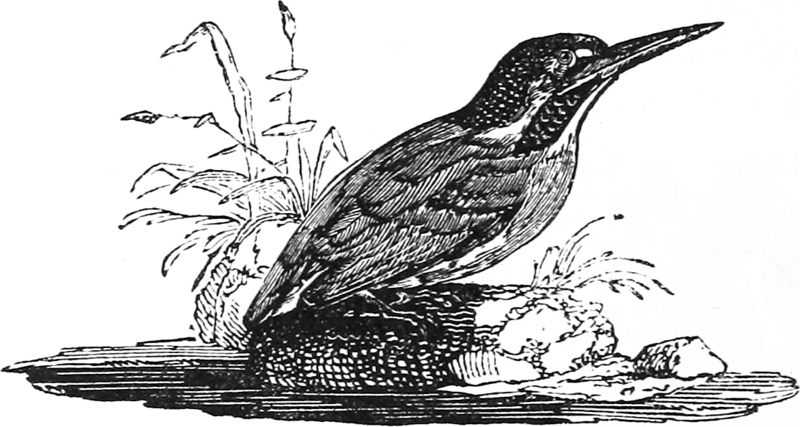
\includegraphics[scale=0.35]{images/Alycon.png}
        \end{figure}
        \vspace{0.5cm}
        \Huge
        \textbf{\textsc{Matematyka Dyskretna}}
        
        \vspace{0.5cm}
        \Large
        \textsc{Wybrane Dowody}
        
        \normalsize
        
        
        \line(1,0){330}
        
        \vspace{1cm}
        \textit{,,Myślę, że 7 punktów na 20 to nie jest zły wynik''}
        \vspace{1cm}

        \textit{\textsc{Popełnione przez}}\\
        \vspace{5mm}

        \textbf{\textsc{Dziurawy Ponton \\ Załatany Ponton \\ Puchaty Pompon \\ Zatopiony Ponton \\ Tonący Ponton \\ Notnop}}

        \vfill

        Kraków \\
        Anno Domini 2023
        
    \end{center}
    
\end{titlepage}


\tableofcontents
\section*{Licencja}
    \begin{figure}[h]
    	\begin{minipage}[c]{0.25\textwidth}
    		
\includegraphics[width=0.7\textwidth]{images/licencja.png}
    	\end{minipage}\hfill
    	\begin{minipage}[c]{0.75\textwidth}
    		\caption*{
    			Ten utwór jest dostępny na 
    			\href{https://creativecommons.org/licenses/by-sa/4.0/}{licencji Creative Commons Uznanie autorstwa
    			na tych samych warunkach 4.0 Międzynarodowe.}
    		}
    	\end{minipage}
    \end{figure}

% Actual content
\mainmatter

\chapter{Kombinatoryka}
 % Żeby nie było syfu to kolejne sekcje dodajemy do chapters/
% A potem includujemy za pomocą \input{chapters/...}

% Używamy \( \) i \[ \] zamiast dolarów -- tak jak się robi w LaTeXu


\documentclass[12pt, a4paper, polish, openany]{book}

% Please, let's familiarize ourselves with notatki.sty and tcs.sty so that we don't reinvent the wheel
\usepackage{notatki}

\fancyhead[L]{\textbf{\textit{MD}}}
\author{
}
\title{TCS and shitposting}


\begin{document}

% Front page and table of contents
\frontmatter

\input{titlepage}

\tableofcontents
\input{license}

% Actual content
\mainmatter

\chapter{Kombinatoryka}
\input{chapters/combinatorics/main}

\chapter{Zasada włączeń i wyłączeń}
\input{chapters/exclusion-inclusion/main}

\chapter{Posety}
\input{chapters/posets/main}

\chapter{Twierdzenie Ramseya}
\input{chapters/ramsey/main}

\chapter{Funkcje tworzące}
\input{chapters/generating_functions/main}

\chapter{Przepływy}
\input{chapters/flows/main}

\chapter{Skojarzenia}
\input{chapters/matchings/main}

\chapter{Kolorowanie grafów}
\input{chapters/graph-coloring/main}

\chapter{Grafy, ale nie kolorowanie}
\input{chapters/graph-misc/main}

\end{document}

\chapter{Zasada włączeń i wyłączeń}
 % Żeby nie było syfu to kolejne sekcje dodajemy do chapters/
% A potem includujemy za pomocą \input{chapters/...}

% Używamy \( \) i \[ \] zamiast dolarów -- tak jak się robi w LaTeXu


\documentclass[12pt, a4paper, polish, openany]{book}

% Please, let's familiarize ourselves with notatki.sty and tcs.sty so that we don't reinvent the wheel
\usepackage{notatki}

\fancyhead[L]{\textbf{\textit{MD}}}
\author{
}
\title{TCS and shitposting}


\begin{document}

% Front page and table of contents
\frontmatter

\input{titlepage}

\tableofcontents
\input{license}

% Actual content
\mainmatter

\chapter{Kombinatoryka}
\input{chapters/combinatorics/main}

\chapter{Zasada włączeń i wyłączeń}
\input{chapters/exclusion-inclusion/main}

\chapter{Posety}
\input{chapters/posets/main}

\chapter{Twierdzenie Ramseya}
\input{chapters/ramsey/main}

\chapter{Funkcje tworzące}
\input{chapters/generating_functions/main}

\chapter{Przepływy}
\input{chapters/flows/main}

\chapter{Skojarzenia}
\input{chapters/matchings/main}

\chapter{Kolorowanie grafów}
\input{chapters/graph-coloring/main}

\chapter{Grafy, ale nie kolorowanie}
\input{chapters/graph-misc/main}

\end{document}

\chapter{Posety}
 % Żeby nie było syfu to kolejne sekcje dodajemy do chapters/
% A potem includujemy za pomocą \input{chapters/...}

% Używamy \( \) i \[ \] zamiast dolarów -- tak jak się robi w LaTeXu


\documentclass[12pt, a4paper, polish, openany]{book}

% Please, let's familiarize ourselves with notatki.sty and tcs.sty so that we don't reinvent the wheel
\usepackage{notatki}

\fancyhead[L]{\textbf{\textit{MD}}}
\author{
}
\title{TCS and shitposting}


\begin{document}

% Front page and table of contents
\frontmatter

\input{titlepage}

\tableofcontents
\input{license}

% Actual content
\mainmatter

\chapter{Kombinatoryka}
\input{chapters/combinatorics/main}

\chapter{Zasada włączeń i wyłączeń}
\input{chapters/exclusion-inclusion/main}

\chapter{Posety}
\input{chapters/posets/main}

\chapter{Twierdzenie Ramseya}
\input{chapters/ramsey/main}

\chapter{Funkcje tworzące}
\input{chapters/generating_functions/main}

\chapter{Przepływy}
\input{chapters/flows/main}

\chapter{Skojarzenia}
\input{chapters/matchings/main}

\chapter{Kolorowanie grafów}
\input{chapters/graph-coloring/main}

\chapter{Grafy, ale nie kolorowanie}
\input{chapters/graph-misc/main}

\end{document}

\chapter{Twierdzenie Ramseya}
 % Żeby nie było syfu to kolejne sekcje dodajemy do chapters/
% A potem includujemy za pomocą \input{chapters/...}

% Używamy \( \) i \[ \] zamiast dolarów -- tak jak się robi w LaTeXu


\documentclass[12pt, a4paper, polish, openany]{book}

% Please, let's familiarize ourselves with notatki.sty and tcs.sty so that we don't reinvent the wheel
\usepackage{notatki}

\fancyhead[L]{\textbf{\textit{MD}}}
\author{
}
\title{TCS and shitposting}


\begin{document}

% Front page and table of contents
\frontmatter

\input{titlepage}

\tableofcontents
\input{license}

% Actual content
\mainmatter

\chapter{Kombinatoryka}
\input{chapters/combinatorics/main}

\chapter{Zasada włączeń i wyłączeń}
\input{chapters/exclusion-inclusion/main}

\chapter{Posety}
\input{chapters/posets/main}

\chapter{Twierdzenie Ramseya}
\input{chapters/ramsey/main}

\chapter{Funkcje tworzące}
\input{chapters/generating_functions/main}

\chapter{Przepływy}
\input{chapters/flows/main}

\chapter{Skojarzenia}
\input{chapters/matchings/main}

\chapter{Kolorowanie grafów}
\input{chapters/graph-coloring/main}

\chapter{Grafy, ale nie kolorowanie}
\input{chapters/graph-misc/main}

\end{document}

\chapter{Funkcje tworzące}
 % Żeby nie było syfu to kolejne sekcje dodajemy do chapters/
% A potem includujemy za pomocą \input{chapters/...}

% Używamy \( \) i \[ \] zamiast dolarów -- tak jak się robi w LaTeXu


\documentclass[12pt, a4paper, polish, openany]{book}

% Please, let's familiarize ourselves with notatki.sty and tcs.sty so that we don't reinvent the wheel
\usepackage{notatki}

\fancyhead[L]{\textbf{\textit{MD}}}
\author{
}
\title{TCS and shitposting}


\begin{document}

% Front page and table of contents
\frontmatter

\input{titlepage}

\tableofcontents
\input{license}

% Actual content
\mainmatter

\chapter{Kombinatoryka}
\input{chapters/combinatorics/main}

\chapter{Zasada włączeń i wyłączeń}
\input{chapters/exclusion-inclusion/main}

\chapter{Posety}
\input{chapters/posets/main}

\chapter{Twierdzenie Ramseya}
\input{chapters/ramsey/main}

\chapter{Funkcje tworzące}
\input{chapters/generating_functions/main}

\chapter{Przepływy}
\input{chapters/flows/main}

\chapter{Skojarzenia}
\input{chapters/matchings/main}

\chapter{Kolorowanie grafów}
\input{chapters/graph-coloring/main}

\chapter{Grafy, ale nie kolorowanie}
\input{chapters/graph-misc/main}

\end{document}

\chapter{Przepływy}
 % Żeby nie było syfu to kolejne sekcje dodajemy do chapters/
% A potem includujemy za pomocą \input{chapters/...}

% Używamy \( \) i \[ \] zamiast dolarów -- tak jak się robi w LaTeXu


\documentclass[12pt, a4paper, polish, openany]{book}

% Please, let's familiarize ourselves with notatki.sty and tcs.sty so that we don't reinvent the wheel
\usepackage{notatki}

\fancyhead[L]{\textbf{\textit{MD}}}
\author{
}
\title{TCS and shitposting}


\begin{document}

% Front page and table of contents
\frontmatter

\input{titlepage}

\tableofcontents
\input{license}

% Actual content
\mainmatter

\chapter{Kombinatoryka}
\input{chapters/combinatorics/main}

\chapter{Zasada włączeń i wyłączeń}
\input{chapters/exclusion-inclusion/main}

\chapter{Posety}
\input{chapters/posets/main}

\chapter{Twierdzenie Ramseya}
\input{chapters/ramsey/main}

\chapter{Funkcje tworzące}
\input{chapters/generating_functions/main}

\chapter{Przepływy}
\input{chapters/flows/main}

\chapter{Skojarzenia}
\input{chapters/matchings/main}

\chapter{Kolorowanie grafów}
\input{chapters/graph-coloring/main}

\chapter{Grafy, ale nie kolorowanie}
\input{chapters/graph-misc/main}

\end{document}

\chapter{Skojarzenia}
 % Żeby nie było syfu to kolejne sekcje dodajemy do chapters/
% A potem includujemy za pomocą \input{chapters/...}

% Używamy \( \) i \[ \] zamiast dolarów -- tak jak się robi w LaTeXu


\documentclass[12pt, a4paper, polish, openany]{book}

% Please, let's familiarize ourselves with notatki.sty and tcs.sty so that we don't reinvent the wheel
\usepackage{notatki}

\fancyhead[L]{\textbf{\textit{MD}}}
\author{
}
\title{TCS and shitposting}


\begin{document}

% Front page and table of contents
\frontmatter

\input{titlepage}

\tableofcontents
\input{license}

% Actual content
\mainmatter

\chapter{Kombinatoryka}
\input{chapters/combinatorics/main}

\chapter{Zasada włączeń i wyłączeń}
\input{chapters/exclusion-inclusion/main}

\chapter{Posety}
\input{chapters/posets/main}

\chapter{Twierdzenie Ramseya}
\input{chapters/ramsey/main}

\chapter{Funkcje tworzące}
\input{chapters/generating_functions/main}

\chapter{Przepływy}
\input{chapters/flows/main}

\chapter{Skojarzenia}
\input{chapters/matchings/main}

\chapter{Kolorowanie grafów}
\input{chapters/graph-coloring/main}

\chapter{Grafy, ale nie kolorowanie}
\input{chapters/graph-misc/main}

\end{document}

\chapter{Kolorowanie grafów}
 % Żeby nie było syfu to kolejne sekcje dodajemy do chapters/
% A potem includujemy za pomocą \input{chapters/...}

% Używamy \( \) i \[ \] zamiast dolarów -- tak jak się robi w LaTeXu


\documentclass[12pt, a4paper, polish, openany]{book}

% Please, let's familiarize ourselves with notatki.sty and tcs.sty so that we don't reinvent the wheel
\usepackage{notatki}

\fancyhead[L]{\textbf{\textit{MD}}}
\author{
}
\title{TCS and shitposting}


\begin{document}

% Front page and table of contents
\frontmatter

\input{titlepage}

\tableofcontents
\input{license}

% Actual content
\mainmatter

\chapter{Kombinatoryka}
\input{chapters/combinatorics/main}

\chapter{Zasada włączeń i wyłączeń}
\input{chapters/exclusion-inclusion/main}

\chapter{Posety}
\input{chapters/posets/main}

\chapter{Twierdzenie Ramseya}
\input{chapters/ramsey/main}

\chapter{Funkcje tworzące}
\input{chapters/generating_functions/main}

\chapter{Przepływy}
\input{chapters/flows/main}

\chapter{Skojarzenia}
\input{chapters/matchings/main}

\chapter{Kolorowanie grafów}
\input{chapters/graph-coloring/main}

\chapter{Grafy, ale nie kolorowanie}
\input{chapters/graph-misc/main}

\end{document}

\chapter{Grafy, ale nie kolorowanie}
 % Żeby nie było syfu to kolejne sekcje dodajemy do chapters/
% A potem includujemy za pomocą \input{chapters/...}

% Używamy \( \) i \[ \] zamiast dolarów -- tak jak się robi w LaTeXu


\documentclass[12pt, a4paper, polish, openany]{book}

% Please, let's familiarize ourselves with notatki.sty and tcs.sty so that we don't reinvent the wheel
\usepackage{notatki}

\fancyhead[L]{\textbf{\textit{MD}}}
\author{
}
\title{TCS and shitposting}


\begin{document}

% Front page and table of contents
\frontmatter

\input{titlepage}

\tableofcontents
\input{license}

% Actual content
\mainmatter

\chapter{Kombinatoryka}
\input{chapters/combinatorics/main}

\chapter{Zasada włączeń i wyłączeń}
\input{chapters/exclusion-inclusion/main}

\chapter{Posety}
\input{chapters/posets/main}

\chapter{Twierdzenie Ramseya}
\input{chapters/ramsey/main}

\chapter{Funkcje tworzące}
\input{chapters/generating_functions/main}

\chapter{Przepływy}
\input{chapters/flows/main}

\chapter{Skojarzenia}
\input{chapters/matchings/main}

\chapter{Kolorowanie grafów}
\input{chapters/graph-coloring/main}

\chapter{Grafy, ale nie kolorowanie}
\input{chapters/graph-misc/main}

\end{document}

\end{document}

\chapter{Przepływy}
 % Żeby nie było syfu to kolejne sekcje dodajemy do chapters/
% A potem includujemy za pomocą \input{chapters/...}

% Używamy \( \) i \[ \] zamiast dolarów -- tak jak się robi w LaTeXu


\documentclass[12pt, a4paper, polish, openany]{book}

% Please, let's familiarize ourselves with notatki.sty and tcs.sty so that we don't reinvent the wheel
\usepackage{notatki}

\fancyhead[L]{\textbf{\textit{MD}}}
\author{
}
\title{TCS and shitposting}


\begin{document}

% Front page and table of contents
\frontmatter

\begin{titlepage} 

    \begin{center}
         \begin{figure}[h]
            \centering
            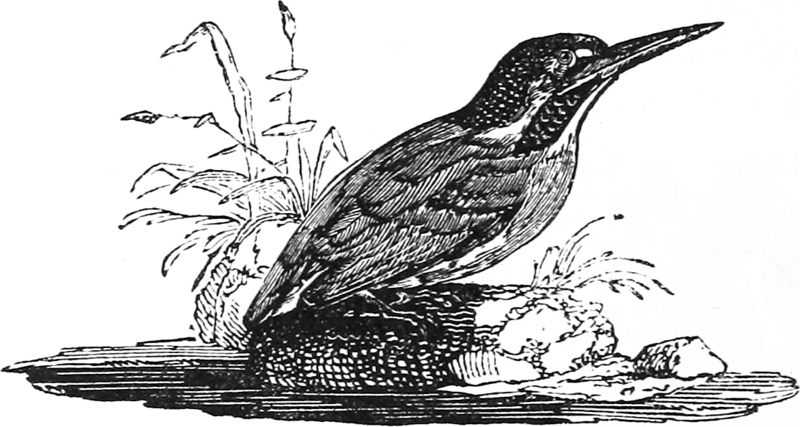
\includegraphics[scale=0.35]{images/Alycon.png}
        \end{figure}
        \vspace{0.5cm}
        \Huge
        \textbf{\textsc{Matematyka Dyskretna}}
        
        \vspace{0.5cm}
        \Large
        \textsc{Wybrane Dowody}
        
        \normalsize
        
        
        \line(1,0){330}
        
        \vspace{1cm}
        \textit{,,Myślę, że 7 punktów na 20 to nie jest zły wynik''}
        \vspace{1cm}

        \textit{\textsc{Popełnione przez}}\\
        \vspace{5mm}

        \textbf{\textsc{Dziurawy Ponton \\ Załatany Ponton \\ Puchaty Pompon \\ Zatopiony Ponton \\ Tonący Ponton \\ Notnop}}

        \vfill

        Kraków \\
        Anno Domini 2023
        
    \end{center}
    
\end{titlepage}


\tableofcontents
\section*{Licencja}
    \begin{figure}[h]
    	\begin{minipage}[c]{0.25\textwidth}
    		
\includegraphics[width=0.7\textwidth]{images/licencja.png}
    	\end{minipage}\hfill
    	\begin{minipage}[c]{0.75\textwidth}
    		\caption*{
    			Ten utwór jest dostępny na 
    			\href{https://creativecommons.org/licenses/by-sa/4.0/}{licencji Creative Commons Uznanie autorstwa
    			na tych samych warunkach 4.0 Międzynarodowe.}
    		}
    	\end{minipage}
    \end{figure}

% Actual content
\mainmatter

\chapter{Kombinatoryka}
 % Żeby nie było syfu to kolejne sekcje dodajemy do chapters/
% A potem includujemy za pomocą \input{chapters/...}

% Używamy \( \) i \[ \] zamiast dolarów -- tak jak się robi w LaTeXu


\documentclass[12pt, a4paper, polish, openany]{book}

% Please, let's familiarize ourselves with notatki.sty and tcs.sty so that we don't reinvent the wheel
\usepackage{notatki}

\fancyhead[L]{\textbf{\textit{MD}}}
\author{
}
\title{TCS and shitposting}


\begin{document}

% Front page and table of contents
\frontmatter

\input{titlepage}

\tableofcontents
\input{license}

% Actual content
\mainmatter

\chapter{Kombinatoryka}
\input{chapters/combinatorics/main}

\chapter{Zasada włączeń i wyłączeń}
\input{chapters/exclusion-inclusion/main}

\chapter{Posety}
\input{chapters/posets/main}

\chapter{Twierdzenie Ramseya}
\input{chapters/ramsey/main}

\chapter{Funkcje tworzące}
\input{chapters/generating_functions/main}

\chapter{Przepływy}
\input{chapters/flows/main}

\chapter{Skojarzenia}
\input{chapters/matchings/main}

\chapter{Kolorowanie grafów}
\input{chapters/graph-coloring/main}

\chapter{Grafy, ale nie kolorowanie}
\input{chapters/graph-misc/main}

\end{document}

\chapter{Zasada włączeń i wyłączeń}
 % Żeby nie było syfu to kolejne sekcje dodajemy do chapters/
% A potem includujemy za pomocą \input{chapters/...}

% Używamy \( \) i \[ \] zamiast dolarów -- tak jak się robi w LaTeXu


\documentclass[12pt, a4paper, polish, openany]{book}

% Please, let's familiarize ourselves with notatki.sty and tcs.sty so that we don't reinvent the wheel
\usepackage{notatki}

\fancyhead[L]{\textbf{\textit{MD}}}
\author{
}
\title{TCS and shitposting}


\begin{document}

% Front page and table of contents
\frontmatter

\input{titlepage}

\tableofcontents
\input{license}

% Actual content
\mainmatter

\chapter{Kombinatoryka}
\input{chapters/combinatorics/main}

\chapter{Zasada włączeń i wyłączeń}
\input{chapters/exclusion-inclusion/main}

\chapter{Posety}
\input{chapters/posets/main}

\chapter{Twierdzenie Ramseya}
\input{chapters/ramsey/main}

\chapter{Funkcje tworzące}
\input{chapters/generating_functions/main}

\chapter{Przepływy}
\input{chapters/flows/main}

\chapter{Skojarzenia}
\input{chapters/matchings/main}

\chapter{Kolorowanie grafów}
\input{chapters/graph-coloring/main}

\chapter{Grafy, ale nie kolorowanie}
\input{chapters/graph-misc/main}

\end{document}

\chapter{Posety}
 % Żeby nie było syfu to kolejne sekcje dodajemy do chapters/
% A potem includujemy za pomocą \input{chapters/...}

% Używamy \( \) i \[ \] zamiast dolarów -- tak jak się robi w LaTeXu


\documentclass[12pt, a4paper, polish, openany]{book}

% Please, let's familiarize ourselves with notatki.sty and tcs.sty so that we don't reinvent the wheel
\usepackage{notatki}

\fancyhead[L]{\textbf{\textit{MD}}}
\author{
}
\title{TCS and shitposting}


\begin{document}

% Front page and table of contents
\frontmatter

\input{titlepage}

\tableofcontents
\input{license}

% Actual content
\mainmatter

\chapter{Kombinatoryka}
\input{chapters/combinatorics/main}

\chapter{Zasada włączeń i wyłączeń}
\input{chapters/exclusion-inclusion/main}

\chapter{Posety}
\input{chapters/posets/main}

\chapter{Twierdzenie Ramseya}
\input{chapters/ramsey/main}

\chapter{Funkcje tworzące}
\input{chapters/generating_functions/main}

\chapter{Przepływy}
\input{chapters/flows/main}

\chapter{Skojarzenia}
\input{chapters/matchings/main}

\chapter{Kolorowanie grafów}
\input{chapters/graph-coloring/main}

\chapter{Grafy, ale nie kolorowanie}
\input{chapters/graph-misc/main}

\end{document}

\chapter{Twierdzenie Ramseya}
 % Żeby nie było syfu to kolejne sekcje dodajemy do chapters/
% A potem includujemy za pomocą \input{chapters/...}

% Używamy \( \) i \[ \] zamiast dolarów -- tak jak się robi w LaTeXu


\documentclass[12pt, a4paper, polish, openany]{book}

% Please, let's familiarize ourselves with notatki.sty and tcs.sty so that we don't reinvent the wheel
\usepackage{notatki}

\fancyhead[L]{\textbf{\textit{MD}}}
\author{
}
\title{TCS and shitposting}


\begin{document}

% Front page and table of contents
\frontmatter

\input{titlepage}

\tableofcontents
\input{license}

% Actual content
\mainmatter

\chapter{Kombinatoryka}
\input{chapters/combinatorics/main}

\chapter{Zasada włączeń i wyłączeń}
\input{chapters/exclusion-inclusion/main}

\chapter{Posety}
\input{chapters/posets/main}

\chapter{Twierdzenie Ramseya}
\input{chapters/ramsey/main}

\chapter{Funkcje tworzące}
\input{chapters/generating_functions/main}

\chapter{Przepływy}
\input{chapters/flows/main}

\chapter{Skojarzenia}
\input{chapters/matchings/main}

\chapter{Kolorowanie grafów}
\input{chapters/graph-coloring/main}

\chapter{Grafy, ale nie kolorowanie}
\input{chapters/graph-misc/main}

\end{document}

\chapter{Funkcje tworzące}
 % Żeby nie było syfu to kolejne sekcje dodajemy do chapters/
% A potem includujemy za pomocą \input{chapters/...}

% Używamy \( \) i \[ \] zamiast dolarów -- tak jak się robi w LaTeXu


\documentclass[12pt, a4paper, polish, openany]{book}

% Please, let's familiarize ourselves with notatki.sty and tcs.sty so that we don't reinvent the wheel
\usepackage{notatki}

\fancyhead[L]{\textbf{\textit{MD}}}
\author{
}
\title{TCS and shitposting}


\begin{document}

% Front page and table of contents
\frontmatter

\input{titlepage}

\tableofcontents
\input{license}

% Actual content
\mainmatter

\chapter{Kombinatoryka}
\input{chapters/combinatorics/main}

\chapter{Zasada włączeń i wyłączeń}
\input{chapters/exclusion-inclusion/main}

\chapter{Posety}
\input{chapters/posets/main}

\chapter{Twierdzenie Ramseya}
\input{chapters/ramsey/main}

\chapter{Funkcje tworzące}
\input{chapters/generating_functions/main}

\chapter{Przepływy}
\input{chapters/flows/main}

\chapter{Skojarzenia}
\input{chapters/matchings/main}

\chapter{Kolorowanie grafów}
\input{chapters/graph-coloring/main}

\chapter{Grafy, ale nie kolorowanie}
\input{chapters/graph-misc/main}

\end{document}

\chapter{Przepływy}
 % Żeby nie było syfu to kolejne sekcje dodajemy do chapters/
% A potem includujemy za pomocą \input{chapters/...}

% Używamy \( \) i \[ \] zamiast dolarów -- tak jak się robi w LaTeXu


\documentclass[12pt, a4paper, polish, openany]{book}

% Please, let's familiarize ourselves with notatki.sty and tcs.sty so that we don't reinvent the wheel
\usepackage{notatki}

\fancyhead[L]{\textbf{\textit{MD}}}
\author{
}
\title{TCS and shitposting}


\begin{document}

% Front page and table of contents
\frontmatter

\input{titlepage}

\tableofcontents
\input{license}

% Actual content
\mainmatter

\chapter{Kombinatoryka}
\input{chapters/combinatorics/main}

\chapter{Zasada włączeń i wyłączeń}
\input{chapters/exclusion-inclusion/main}

\chapter{Posety}
\input{chapters/posets/main}

\chapter{Twierdzenie Ramseya}
\input{chapters/ramsey/main}

\chapter{Funkcje tworzące}
\input{chapters/generating_functions/main}

\chapter{Przepływy}
\input{chapters/flows/main}

\chapter{Skojarzenia}
\input{chapters/matchings/main}

\chapter{Kolorowanie grafów}
\input{chapters/graph-coloring/main}

\chapter{Grafy, ale nie kolorowanie}
\input{chapters/graph-misc/main}

\end{document}

\chapter{Skojarzenia}
 % Żeby nie było syfu to kolejne sekcje dodajemy do chapters/
% A potem includujemy za pomocą \input{chapters/...}

% Używamy \( \) i \[ \] zamiast dolarów -- tak jak się robi w LaTeXu


\documentclass[12pt, a4paper, polish, openany]{book}

% Please, let's familiarize ourselves with notatki.sty and tcs.sty so that we don't reinvent the wheel
\usepackage{notatki}

\fancyhead[L]{\textbf{\textit{MD}}}
\author{
}
\title{TCS and shitposting}


\begin{document}

% Front page and table of contents
\frontmatter

\input{titlepage}

\tableofcontents
\input{license}

% Actual content
\mainmatter

\chapter{Kombinatoryka}
\input{chapters/combinatorics/main}

\chapter{Zasada włączeń i wyłączeń}
\input{chapters/exclusion-inclusion/main}

\chapter{Posety}
\input{chapters/posets/main}

\chapter{Twierdzenie Ramseya}
\input{chapters/ramsey/main}

\chapter{Funkcje tworzące}
\input{chapters/generating_functions/main}

\chapter{Przepływy}
\input{chapters/flows/main}

\chapter{Skojarzenia}
\input{chapters/matchings/main}

\chapter{Kolorowanie grafów}
\input{chapters/graph-coloring/main}

\chapter{Grafy, ale nie kolorowanie}
\input{chapters/graph-misc/main}

\end{document}

\chapter{Kolorowanie grafów}
 % Żeby nie było syfu to kolejne sekcje dodajemy do chapters/
% A potem includujemy za pomocą \input{chapters/...}

% Używamy \( \) i \[ \] zamiast dolarów -- tak jak się robi w LaTeXu


\documentclass[12pt, a4paper, polish, openany]{book}

% Please, let's familiarize ourselves with notatki.sty and tcs.sty so that we don't reinvent the wheel
\usepackage{notatki}

\fancyhead[L]{\textbf{\textit{MD}}}
\author{
}
\title{TCS and shitposting}


\begin{document}

% Front page and table of contents
\frontmatter

\input{titlepage}

\tableofcontents
\input{license}

% Actual content
\mainmatter

\chapter{Kombinatoryka}
\input{chapters/combinatorics/main}

\chapter{Zasada włączeń i wyłączeń}
\input{chapters/exclusion-inclusion/main}

\chapter{Posety}
\input{chapters/posets/main}

\chapter{Twierdzenie Ramseya}
\input{chapters/ramsey/main}

\chapter{Funkcje tworzące}
\input{chapters/generating_functions/main}

\chapter{Przepływy}
\input{chapters/flows/main}

\chapter{Skojarzenia}
\input{chapters/matchings/main}

\chapter{Kolorowanie grafów}
\input{chapters/graph-coloring/main}

\chapter{Grafy, ale nie kolorowanie}
\input{chapters/graph-misc/main}

\end{document}

\chapter{Grafy, ale nie kolorowanie}
 % Żeby nie było syfu to kolejne sekcje dodajemy do chapters/
% A potem includujemy za pomocą \input{chapters/...}

% Używamy \( \) i \[ \] zamiast dolarów -- tak jak się robi w LaTeXu


\documentclass[12pt, a4paper, polish, openany]{book}

% Please, let's familiarize ourselves with notatki.sty and tcs.sty so that we don't reinvent the wheel
\usepackage{notatki}

\fancyhead[L]{\textbf{\textit{MD}}}
\author{
}
\title{TCS and shitposting}


\begin{document}

% Front page and table of contents
\frontmatter

\input{titlepage}

\tableofcontents
\input{license}

% Actual content
\mainmatter

\chapter{Kombinatoryka}
\input{chapters/combinatorics/main}

\chapter{Zasada włączeń i wyłączeń}
\input{chapters/exclusion-inclusion/main}

\chapter{Posety}
\input{chapters/posets/main}

\chapter{Twierdzenie Ramseya}
\input{chapters/ramsey/main}

\chapter{Funkcje tworzące}
\input{chapters/generating_functions/main}

\chapter{Przepływy}
\input{chapters/flows/main}

\chapter{Skojarzenia}
\input{chapters/matchings/main}

\chapter{Kolorowanie grafów}
\input{chapters/graph-coloring/main}

\chapter{Grafy, ale nie kolorowanie}
\input{chapters/graph-misc/main}

\end{document}

\end{document}

\chapter{Skojarzenia}
 % Żeby nie było syfu to kolejne sekcje dodajemy do chapters/
% A potem includujemy za pomocą \input{chapters/...}

% Używamy \( \) i \[ \] zamiast dolarów -- tak jak się robi w LaTeXu


\documentclass[12pt, a4paper, polish, openany]{book}

% Please, let's familiarize ourselves with notatki.sty and tcs.sty so that we don't reinvent the wheel
\usepackage{notatki}

\fancyhead[L]{\textbf{\textit{MD}}}
\author{
}
\title{TCS and shitposting}


\begin{document}

% Front page and table of contents
\frontmatter

\begin{titlepage} 

    \begin{center}
         \begin{figure}[h]
            \centering
            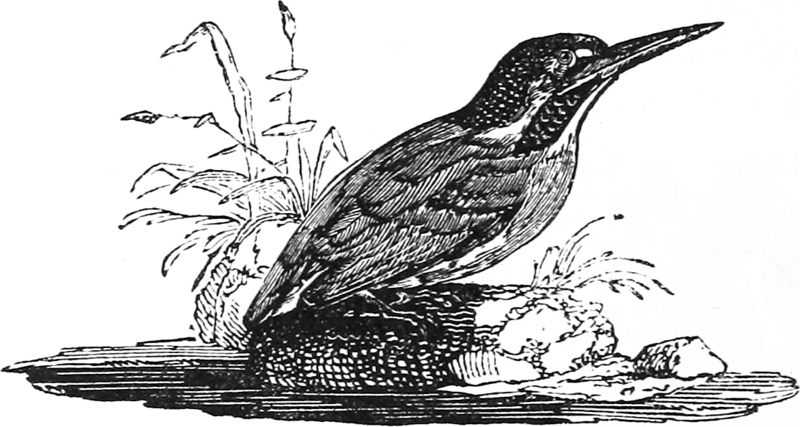
\includegraphics[scale=0.35]{images/Alycon.png}
        \end{figure}
        \vspace{0.5cm}
        \Huge
        \textbf{\textsc{Matematyka Dyskretna}}
        
        \vspace{0.5cm}
        \Large
        \textsc{Wybrane Dowody}
        
        \normalsize
        
        
        \line(1,0){330}
        
        \vspace{1cm}
        \textit{,,Myślę, że 7 punktów na 20 to nie jest zły wynik''}
        \vspace{1cm}

        \textit{\textsc{Popełnione przez}}\\
        \vspace{5mm}

        \textbf{\textsc{Dziurawy Ponton \\ Załatany Ponton \\ Puchaty Pompon \\ Zatopiony Ponton \\ Tonący Ponton \\ Notnop}}

        \vfill

        Kraków \\
        Anno Domini 2023
        
    \end{center}
    
\end{titlepage}


\tableofcontents
\section*{Licencja}
    \begin{figure}[h]
    	\begin{minipage}[c]{0.25\textwidth}
    		
\includegraphics[width=0.7\textwidth]{images/licencja.png}
    	\end{minipage}\hfill
    	\begin{minipage}[c]{0.75\textwidth}
    		\caption*{
    			Ten utwór jest dostępny na 
    			\href{https://creativecommons.org/licenses/by-sa/4.0/}{licencji Creative Commons Uznanie autorstwa
    			na tych samych warunkach 4.0 Międzynarodowe.}
    		}
    	\end{minipage}
    \end{figure}

% Actual content
\mainmatter

\chapter{Kombinatoryka}
 % Żeby nie było syfu to kolejne sekcje dodajemy do chapters/
% A potem includujemy za pomocą \input{chapters/...}

% Używamy \( \) i \[ \] zamiast dolarów -- tak jak się robi w LaTeXu


\documentclass[12pt, a4paper, polish, openany]{book}

% Please, let's familiarize ourselves with notatki.sty and tcs.sty so that we don't reinvent the wheel
\usepackage{notatki}

\fancyhead[L]{\textbf{\textit{MD}}}
\author{
}
\title{TCS and shitposting}


\begin{document}

% Front page and table of contents
\frontmatter

\input{titlepage}

\tableofcontents
\input{license}

% Actual content
\mainmatter

\chapter{Kombinatoryka}
\input{chapters/combinatorics/main}

\chapter{Zasada włączeń i wyłączeń}
\input{chapters/exclusion-inclusion/main}

\chapter{Posety}
\input{chapters/posets/main}

\chapter{Twierdzenie Ramseya}
\input{chapters/ramsey/main}

\chapter{Funkcje tworzące}
\input{chapters/generating_functions/main}

\chapter{Przepływy}
\input{chapters/flows/main}

\chapter{Skojarzenia}
\input{chapters/matchings/main}

\chapter{Kolorowanie grafów}
\input{chapters/graph-coloring/main}

\chapter{Grafy, ale nie kolorowanie}
\input{chapters/graph-misc/main}

\end{document}

\chapter{Zasada włączeń i wyłączeń}
 % Żeby nie było syfu to kolejne sekcje dodajemy do chapters/
% A potem includujemy za pomocą \input{chapters/...}

% Używamy \( \) i \[ \] zamiast dolarów -- tak jak się robi w LaTeXu


\documentclass[12pt, a4paper, polish, openany]{book}

% Please, let's familiarize ourselves with notatki.sty and tcs.sty so that we don't reinvent the wheel
\usepackage{notatki}

\fancyhead[L]{\textbf{\textit{MD}}}
\author{
}
\title{TCS and shitposting}


\begin{document}

% Front page and table of contents
\frontmatter

\input{titlepage}

\tableofcontents
\input{license}

% Actual content
\mainmatter

\chapter{Kombinatoryka}
\input{chapters/combinatorics/main}

\chapter{Zasada włączeń i wyłączeń}
\input{chapters/exclusion-inclusion/main}

\chapter{Posety}
\input{chapters/posets/main}

\chapter{Twierdzenie Ramseya}
\input{chapters/ramsey/main}

\chapter{Funkcje tworzące}
\input{chapters/generating_functions/main}

\chapter{Przepływy}
\input{chapters/flows/main}

\chapter{Skojarzenia}
\input{chapters/matchings/main}

\chapter{Kolorowanie grafów}
\input{chapters/graph-coloring/main}

\chapter{Grafy, ale nie kolorowanie}
\input{chapters/graph-misc/main}

\end{document}

\chapter{Posety}
 % Żeby nie było syfu to kolejne sekcje dodajemy do chapters/
% A potem includujemy za pomocą \input{chapters/...}

% Używamy \( \) i \[ \] zamiast dolarów -- tak jak się robi w LaTeXu


\documentclass[12pt, a4paper, polish, openany]{book}

% Please, let's familiarize ourselves with notatki.sty and tcs.sty so that we don't reinvent the wheel
\usepackage{notatki}

\fancyhead[L]{\textbf{\textit{MD}}}
\author{
}
\title{TCS and shitposting}


\begin{document}

% Front page and table of contents
\frontmatter

\input{titlepage}

\tableofcontents
\input{license}

% Actual content
\mainmatter

\chapter{Kombinatoryka}
\input{chapters/combinatorics/main}

\chapter{Zasada włączeń i wyłączeń}
\input{chapters/exclusion-inclusion/main}

\chapter{Posety}
\input{chapters/posets/main}

\chapter{Twierdzenie Ramseya}
\input{chapters/ramsey/main}

\chapter{Funkcje tworzące}
\input{chapters/generating_functions/main}

\chapter{Przepływy}
\input{chapters/flows/main}

\chapter{Skojarzenia}
\input{chapters/matchings/main}

\chapter{Kolorowanie grafów}
\input{chapters/graph-coloring/main}

\chapter{Grafy, ale nie kolorowanie}
\input{chapters/graph-misc/main}

\end{document}

\chapter{Twierdzenie Ramseya}
 % Żeby nie było syfu to kolejne sekcje dodajemy do chapters/
% A potem includujemy za pomocą \input{chapters/...}

% Używamy \( \) i \[ \] zamiast dolarów -- tak jak się robi w LaTeXu


\documentclass[12pt, a4paper, polish, openany]{book}

% Please, let's familiarize ourselves with notatki.sty and tcs.sty so that we don't reinvent the wheel
\usepackage{notatki}

\fancyhead[L]{\textbf{\textit{MD}}}
\author{
}
\title{TCS and shitposting}


\begin{document}

% Front page and table of contents
\frontmatter

\input{titlepage}

\tableofcontents
\input{license}

% Actual content
\mainmatter

\chapter{Kombinatoryka}
\input{chapters/combinatorics/main}

\chapter{Zasada włączeń i wyłączeń}
\input{chapters/exclusion-inclusion/main}

\chapter{Posety}
\input{chapters/posets/main}

\chapter{Twierdzenie Ramseya}
\input{chapters/ramsey/main}

\chapter{Funkcje tworzące}
\input{chapters/generating_functions/main}

\chapter{Przepływy}
\input{chapters/flows/main}

\chapter{Skojarzenia}
\input{chapters/matchings/main}

\chapter{Kolorowanie grafów}
\input{chapters/graph-coloring/main}

\chapter{Grafy, ale nie kolorowanie}
\input{chapters/graph-misc/main}

\end{document}

\chapter{Funkcje tworzące}
 % Żeby nie było syfu to kolejne sekcje dodajemy do chapters/
% A potem includujemy za pomocą \input{chapters/...}

% Używamy \( \) i \[ \] zamiast dolarów -- tak jak się robi w LaTeXu


\documentclass[12pt, a4paper, polish, openany]{book}

% Please, let's familiarize ourselves with notatki.sty and tcs.sty so that we don't reinvent the wheel
\usepackage{notatki}

\fancyhead[L]{\textbf{\textit{MD}}}
\author{
}
\title{TCS and shitposting}


\begin{document}

% Front page and table of contents
\frontmatter

\input{titlepage}

\tableofcontents
\input{license}

% Actual content
\mainmatter

\chapter{Kombinatoryka}
\input{chapters/combinatorics/main}

\chapter{Zasada włączeń i wyłączeń}
\input{chapters/exclusion-inclusion/main}

\chapter{Posety}
\input{chapters/posets/main}

\chapter{Twierdzenie Ramseya}
\input{chapters/ramsey/main}

\chapter{Funkcje tworzące}
\input{chapters/generating_functions/main}

\chapter{Przepływy}
\input{chapters/flows/main}

\chapter{Skojarzenia}
\input{chapters/matchings/main}

\chapter{Kolorowanie grafów}
\input{chapters/graph-coloring/main}

\chapter{Grafy, ale nie kolorowanie}
\input{chapters/graph-misc/main}

\end{document}

\chapter{Przepływy}
 % Żeby nie było syfu to kolejne sekcje dodajemy do chapters/
% A potem includujemy za pomocą \input{chapters/...}

% Używamy \( \) i \[ \] zamiast dolarów -- tak jak się robi w LaTeXu


\documentclass[12pt, a4paper, polish, openany]{book}

% Please, let's familiarize ourselves with notatki.sty and tcs.sty so that we don't reinvent the wheel
\usepackage{notatki}

\fancyhead[L]{\textbf{\textit{MD}}}
\author{
}
\title{TCS and shitposting}


\begin{document}

% Front page and table of contents
\frontmatter

\input{titlepage}

\tableofcontents
\input{license}

% Actual content
\mainmatter

\chapter{Kombinatoryka}
\input{chapters/combinatorics/main}

\chapter{Zasada włączeń i wyłączeń}
\input{chapters/exclusion-inclusion/main}

\chapter{Posety}
\input{chapters/posets/main}

\chapter{Twierdzenie Ramseya}
\input{chapters/ramsey/main}

\chapter{Funkcje tworzące}
\input{chapters/generating_functions/main}

\chapter{Przepływy}
\input{chapters/flows/main}

\chapter{Skojarzenia}
\input{chapters/matchings/main}

\chapter{Kolorowanie grafów}
\input{chapters/graph-coloring/main}

\chapter{Grafy, ale nie kolorowanie}
\input{chapters/graph-misc/main}

\end{document}

\chapter{Skojarzenia}
 % Żeby nie było syfu to kolejne sekcje dodajemy do chapters/
% A potem includujemy za pomocą \input{chapters/...}

% Używamy \( \) i \[ \] zamiast dolarów -- tak jak się robi w LaTeXu


\documentclass[12pt, a4paper, polish, openany]{book}

% Please, let's familiarize ourselves with notatki.sty and tcs.sty so that we don't reinvent the wheel
\usepackage{notatki}

\fancyhead[L]{\textbf{\textit{MD}}}
\author{
}
\title{TCS and shitposting}


\begin{document}

% Front page and table of contents
\frontmatter

\input{titlepage}

\tableofcontents
\input{license}

% Actual content
\mainmatter

\chapter{Kombinatoryka}
\input{chapters/combinatorics/main}

\chapter{Zasada włączeń i wyłączeń}
\input{chapters/exclusion-inclusion/main}

\chapter{Posety}
\input{chapters/posets/main}

\chapter{Twierdzenie Ramseya}
\input{chapters/ramsey/main}

\chapter{Funkcje tworzące}
\input{chapters/generating_functions/main}

\chapter{Przepływy}
\input{chapters/flows/main}

\chapter{Skojarzenia}
\input{chapters/matchings/main}

\chapter{Kolorowanie grafów}
\input{chapters/graph-coloring/main}

\chapter{Grafy, ale nie kolorowanie}
\input{chapters/graph-misc/main}

\end{document}

\chapter{Kolorowanie grafów}
 % Żeby nie było syfu to kolejne sekcje dodajemy do chapters/
% A potem includujemy za pomocą \input{chapters/...}

% Używamy \( \) i \[ \] zamiast dolarów -- tak jak się robi w LaTeXu


\documentclass[12pt, a4paper, polish, openany]{book}

% Please, let's familiarize ourselves with notatki.sty and tcs.sty so that we don't reinvent the wheel
\usepackage{notatki}

\fancyhead[L]{\textbf{\textit{MD}}}
\author{
}
\title{TCS and shitposting}


\begin{document}

% Front page and table of contents
\frontmatter

\input{titlepage}

\tableofcontents
\input{license}

% Actual content
\mainmatter

\chapter{Kombinatoryka}
\input{chapters/combinatorics/main}

\chapter{Zasada włączeń i wyłączeń}
\input{chapters/exclusion-inclusion/main}

\chapter{Posety}
\input{chapters/posets/main}

\chapter{Twierdzenie Ramseya}
\input{chapters/ramsey/main}

\chapter{Funkcje tworzące}
\input{chapters/generating_functions/main}

\chapter{Przepływy}
\input{chapters/flows/main}

\chapter{Skojarzenia}
\input{chapters/matchings/main}

\chapter{Kolorowanie grafów}
\input{chapters/graph-coloring/main}

\chapter{Grafy, ale nie kolorowanie}
\input{chapters/graph-misc/main}

\end{document}

\chapter{Grafy, ale nie kolorowanie}
 % Żeby nie było syfu to kolejne sekcje dodajemy do chapters/
% A potem includujemy za pomocą \input{chapters/...}

% Używamy \( \) i \[ \] zamiast dolarów -- tak jak się robi w LaTeXu


\documentclass[12pt, a4paper, polish, openany]{book}

% Please, let's familiarize ourselves with notatki.sty and tcs.sty so that we don't reinvent the wheel
\usepackage{notatki}

\fancyhead[L]{\textbf{\textit{MD}}}
\author{
}
\title{TCS and shitposting}


\begin{document}

% Front page and table of contents
\frontmatter

\input{titlepage}

\tableofcontents
\input{license}

% Actual content
\mainmatter

\chapter{Kombinatoryka}
\input{chapters/combinatorics/main}

\chapter{Zasada włączeń i wyłączeń}
\input{chapters/exclusion-inclusion/main}

\chapter{Posety}
\input{chapters/posets/main}

\chapter{Twierdzenie Ramseya}
\input{chapters/ramsey/main}

\chapter{Funkcje tworzące}
\input{chapters/generating_functions/main}

\chapter{Przepływy}
\input{chapters/flows/main}

\chapter{Skojarzenia}
\input{chapters/matchings/main}

\chapter{Kolorowanie grafów}
\input{chapters/graph-coloring/main}

\chapter{Grafy, ale nie kolorowanie}
\input{chapters/graph-misc/main}

\end{document}

\end{document}

\chapter{Kolorowanie grafów}
 % Żeby nie było syfu to kolejne sekcje dodajemy do chapters/
% A potem includujemy za pomocą \input{chapters/...}

% Używamy \( \) i \[ \] zamiast dolarów -- tak jak się robi w LaTeXu


\documentclass[12pt, a4paper, polish, openany]{book}

% Please, let's familiarize ourselves with notatki.sty and tcs.sty so that we don't reinvent the wheel
\usepackage{notatki}

\fancyhead[L]{\textbf{\textit{MD}}}
\author{
}
\title{TCS and shitposting}


\begin{document}

% Front page and table of contents
\frontmatter

\begin{titlepage} 

    \begin{center}
         \begin{figure}[h]
            \centering
            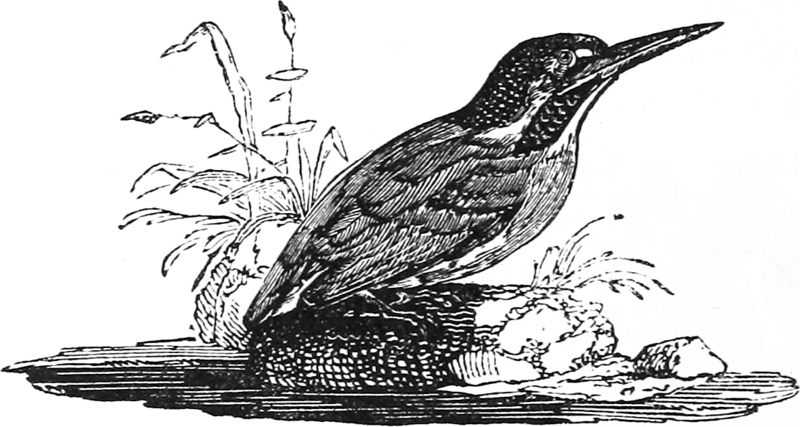
\includegraphics[scale=0.35]{images/Alycon.png}
        \end{figure}
        \vspace{0.5cm}
        \Huge
        \textbf{\textsc{Matematyka Dyskretna}}
        
        \vspace{0.5cm}
        \Large
        \textsc{Wybrane Dowody}
        
        \normalsize
        
        
        \line(1,0){330}
        
        \vspace{1cm}
        \textit{,,Myślę, że 7 punktów na 20 to nie jest zły wynik''}
        \vspace{1cm}

        \textit{\textsc{Popełnione przez}}\\
        \vspace{5mm}

        \textbf{\textsc{Dziurawy Ponton \\ Załatany Ponton \\ Puchaty Pompon \\ Zatopiony Ponton \\ Tonący Ponton \\ Notnop}}

        \vfill

        Kraków \\
        Anno Domini 2023
        
    \end{center}
    
\end{titlepage}


\tableofcontents
\section*{Licencja}
    \begin{figure}[h]
    	\begin{minipage}[c]{0.25\textwidth}
    		
\includegraphics[width=0.7\textwidth]{images/licencja.png}
    	\end{minipage}\hfill
    	\begin{minipage}[c]{0.75\textwidth}
    		\caption*{
    			Ten utwór jest dostępny na 
    			\href{https://creativecommons.org/licenses/by-sa/4.0/}{licencji Creative Commons Uznanie autorstwa
    			na tych samych warunkach 4.0 Międzynarodowe.}
    		}
    	\end{minipage}
    \end{figure}

% Actual content
\mainmatter

\chapter{Kombinatoryka}
 % Żeby nie było syfu to kolejne sekcje dodajemy do chapters/
% A potem includujemy za pomocą \input{chapters/...}

% Używamy \( \) i \[ \] zamiast dolarów -- tak jak się robi w LaTeXu


\documentclass[12pt, a4paper, polish, openany]{book}

% Please, let's familiarize ourselves with notatki.sty and tcs.sty so that we don't reinvent the wheel
\usepackage{notatki}

\fancyhead[L]{\textbf{\textit{MD}}}
\author{
}
\title{TCS and shitposting}


\begin{document}

% Front page and table of contents
\frontmatter

\input{titlepage}

\tableofcontents
\input{license}

% Actual content
\mainmatter

\chapter{Kombinatoryka}
\input{chapters/combinatorics/main}

\chapter{Zasada włączeń i wyłączeń}
\input{chapters/exclusion-inclusion/main}

\chapter{Posety}
\input{chapters/posets/main}

\chapter{Twierdzenie Ramseya}
\input{chapters/ramsey/main}

\chapter{Funkcje tworzące}
\input{chapters/generating_functions/main}

\chapter{Przepływy}
\input{chapters/flows/main}

\chapter{Skojarzenia}
\input{chapters/matchings/main}

\chapter{Kolorowanie grafów}
\input{chapters/graph-coloring/main}

\chapter{Grafy, ale nie kolorowanie}
\input{chapters/graph-misc/main}

\end{document}

\chapter{Zasada włączeń i wyłączeń}
 % Żeby nie było syfu to kolejne sekcje dodajemy do chapters/
% A potem includujemy za pomocą \input{chapters/...}

% Używamy \( \) i \[ \] zamiast dolarów -- tak jak się robi w LaTeXu


\documentclass[12pt, a4paper, polish, openany]{book}

% Please, let's familiarize ourselves with notatki.sty and tcs.sty so that we don't reinvent the wheel
\usepackage{notatki}

\fancyhead[L]{\textbf{\textit{MD}}}
\author{
}
\title{TCS and shitposting}


\begin{document}

% Front page and table of contents
\frontmatter

\input{titlepage}

\tableofcontents
\input{license}

% Actual content
\mainmatter

\chapter{Kombinatoryka}
\input{chapters/combinatorics/main}

\chapter{Zasada włączeń i wyłączeń}
\input{chapters/exclusion-inclusion/main}

\chapter{Posety}
\input{chapters/posets/main}

\chapter{Twierdzenie Ramseya}
\input{chapters/ramsey/main}

\chapter{Funkcje tworzące}
\input{chapters/generating_functions/main}

\chapter{Przepływy}
\input{chapters/flows/main}

\chapter{Skojarzenia}
\input{chapters/matchings/main}

\chapter{Kolorowanie grafów}
\input{chapters/graph-coloring/main}

\chapter{Grafy, ale nie kolorowanie}
\input{chapters/graph-misc/main}

\end{document}

\chapter{Posety}
 % Żeby nie było syfu to kolejne sekcje dodajemy do chapters/
% A potem includujemy za pomocą \input{chapters/...}

% Używamy \( \) i \[ \] zamiast dolarów -- tak jak się robi w LaTeXu


\documentclass[12pt, a4paper, polish, openany]{book}

% Please, let's familiarize ourselves with notatki.sty and tcs.sty so that we don't reinvent the wheel
\usepackage{notatki}

\fancyhead[L]{\textbf{\textit{MD}}}
\author{
}
\title{TCS and shitposting}


\begin{document}

% Front page and table of contents
\frontmatter

\input{titlepage}

\tableofcontents
\input{license}

% Actual content
\mainmatter

\chapter{Kombinatoryka}
\input{chapters/combinatorics/main}

\chapter{Zasada włączeń i wyłączeń}
\input{chapters/exclusion-inclusion/main}

\chapter{Posety}
\input{chapters/posets/main}

\chapter{Twierdzenie Ramseya}
\input{chapters/ramsey/main}

\chapter{Funkcje tworzące}
\input{chapters/generating_functions/main}

\chapter{Przepływy}
\input{chapters/flows/main}

\chapter{Skojarzenia}
\input{chapters/matchings/main}

\chapter{Kolorowanie grafów}
\input{chapters/graph-coloring/main}

\chapter{Grafy, ale nie kolorowanie}
\input{chapters/graph-misc/main}

\end{document}

\chapter{Twierdzenie Ramseya}
 % Żeby nie było syfu to kolejne sekcje dodajemy do chapters/
% A potem includujemy za pomocą \input{chapters/...}

% Używamy \( \) i \[ \] zamiast dolarów -- tak jak się robi w LaTeXu


\documentclass[12pt, a4paper, polish, openany]{book}

% Please, let's familiarize ourselves with notatki.sty and tcs.sty so that we don't reinvent the wheel
\usepackage{notatki}

\fancyhead[L]{\textbf{\textit{MD}}}
\author{
}
\title{TCS and shitposting}


\begin{document}

% Front page and table of contents
\frontmatter

\input{titlepage}

\tableofcontents
\input{license}

% Actual content
\mainmatter

\chapter{Kombinatoryka}
\input{chapters/combinatorics/main}

\chapter{Zasada włączeń i wyłączeń}
\input{chapters/exclusion-inclusion/main}

\chapter{Posety}
\input{chapters/posets/main}

\chapter{Twierdzenie Ramseya}
\input{chapters/ramsey/main}

\chapter{Funkcje tworzące}
\input{chapters/generating_functions/main}

\chapter{Przepływy}
\input{chapters/flows/main}

\chapter{Skojarzenia}
\input{chapters/matchings/main}

\chapter{Kolorowanie grafów}
\input{chapters/graph-coloring/main}

\chapter{Grafy, ale nie kolorowanie}
\input{chapters/graph-misc/main}

\end{document}

\chapter{Funkcje tworzące}
 % Żeby nie było syfu to kolejne sekcje dodajemy do chapters/
% A potem includujemy za pomocą \input{chapters/...}

% Używamy \( \) i \[ \] zamiast dolarów -- tak jak się robi w LaTeXu


\documentclass[12pt, a4paper, polish, openany]{book}

% Please, let's familiarize ourselves with notatki.sty and tcs.sty so that we don't reinvent the wheel
\usepackage{notatki}

\fancyhead[L]{\textbf{\textit{MD}}}
\author{
}
\title{TCS and shitposting}


\begin{document}

% Front page and table of contents
\frontmatter

\input{titlepage}

\tableofcontents
\input{license}

% Actual content
\mainmatter

\chapter{Kombinatoryka}
\input{chapters/combinatorics/main}

\chapter{Zasada włączeń i wyłączeń}
\input{chapters/exclusion-inclusion/main}

\chapter{Posety}
\input{chapters/posets/main}

\chapter{Twierdzenie Ramseya}
\input{chapters/ramsey/main}

\chapter{Funkcje tworzące}
\input{chapters/generating_functions/main}

\chapter{Przepływy}
\input{chapters/flows/main}

\chapter{Skojarzenia}
\input{chapters/matchings/main}

\chapter{Kolorowanie grafów}
\input{chapters/graph-coloring/main}

\chapter{Grafy, ale nie kolorowanie}
\input{chapters/graph-misc/main}

\end{document}

\chapter{Przepływy}
 % Żeby nie było syfu to kolejne sekcje dodajemy do chapters/
% A potem includujemy za pomocą \input{chapters/...}

% Używamy \( \) i \[ \] zamiast dolarów -- tak jak się robi w LaTeXu


\documentclass[12pt, a4paper, polish, openany]{book}

% Please, let's familiarize ourselves with notatki.sty and tcs.sty so that we don't reinvent the wheel
\usepackage{notatki}

\fancyhead[L]{\textbf{\textit{MD}}}
\author{
}
\title{TCS and shitposting}


\begin{document}

% Front page and table of contents
\frontmatter

\input{titlepage}

\tableofcontents
\input{license}

% Actual content
\mainmatter

\chapter{Kombinatoryka}
\input{chapters/combinatorics/main}

\chapter{Zasada włączeń i wyłączeń}
\input{chapters/exclusion-inclusion/main}

\chapter{Posety}
\input{chapters/posets/main}

\chapter{Twierdzenie Ramseya}
\input{chapters/ramsey/main}

\chapter{Funkcje tworzące}
\input{chapters/generating_functions/main}

\chapter{Przepływy}
\input{chapters/flows/main}

\chapter{Skojarzenia}
\input{chapters/matchings/main}

\chapter{Kolorowanie grafów}
\input{chapters/graph-coloring/main}

\chapter{Grafy, ale nie kolorowanie}
\input{chapters/graph-misc/main}

\end{document}

\chapter{Skojarzenia}
 % Żeby nie było syfu to kolejne sekcje dodajemy do chapters/
% A potem includujemy za pomocą \input{chapters/...}

% Używamy \( \) i \[ \] zamiast dolarów -- tak jak się robi w LaTeXu


\documentclass[12pt, a4paper, polish, openany]{book}

% Please, let's familiarize ourselves with notatki.sty and tcs.sty so that we don't reinvent the wheel
\usepackage{notatki}

\fancyhead[L]{\textbf{\textit{MD}}}
\author{
}
\title{TCS and shitposting}


\begin{document}

% Front page and table of contents
\frontmatter

\input{titlepage}

\tableofcontents
\input{license}

% Actual content
\mainmatter

\chapter{Kombinatoryka}
\input{chapters/combinatorics/main}

\chapter{Zasada włączeń i wyłączeń}
\input{chapters/exclusion-inclusion/main}

\chapter{Posety}
\input{chapters/posets/main}

\chapter{Twierdzenie Ramseya}
\input{chapters/ramsey/main}

\chapter{Funkcje tworzące}
\input{chapters/generating_functions/main}

\chapter{Przepływy}
\input{chapters/flows/main}

\chapter{Skojarzenia}
\input{chapters/matchings/main}

\chapter{Kolorowanie grafów}
\input{chapters/graph-coloring/main}

\chapter{Grafy, ale nie kolorowanie}
\input{chapters/graph-misc/main}

\end{document}

\chapter{Kolorowanie grafów}
 % Żeby nie było syfu to kolejne sekcje dodajemy do chapters/
% A potem includujemy za pomocą \input{chapters/...}

% Używamy \( \) i \[ \] zamiast dolarów -- tak jak się robi w LaTeXu


\documentclass[12pt, a4paper, polish, openany]{book}

% Please, let's familiarize ourselves with notatki.sty and tcs.sty so that we don't reinvent the wheel
\usepackage{notatki}

\fancyhead[L]{\textbf{\textit{MD}}}
\author{
}
\title{TCS and shitposting}


\begin{document}

% Front page and table of contents
\frontmatter

\input{titlepage}

\tableofcontents
\input{license}

% Actual content
\mainmatter

\chapter{Kombinatoryka}
\input{chapters/combinatorics/main}

\chapter{Zasada włączeń i wyłączeń}
\input{chapters/exclusion-inclusion/main}

\chapter{Posety}
\input{chapters/posets/main}

\chapter{Twierdzenie Ramseya}
\input{chapters/ramsey/main}

\chapter{Funkcje tworzące}
\input{chapters/generating_functions/main}

\chapter{Przepływy}
\input{chapters/flows/main}

\chapter{Skojarzenia}
\input{chapters/matchings/main}

\chapter{Kolorowanie grafów}
\input{chapters/graph-coloring/main}

\chapter{Grafy, ale nie kolorowanie}
\input{chapters/graph-misc/main}

\end{document}

\chapter{Grafy, ale nie kolorowanie}
 % Żeby nie było syfu to kolejne sekcje dodajemy do chapters/
% A potem includujemy za pomocą \input{chapters/...}

% Używamy \( \) i \[ \] zamiast dolarów -- tak jak się robi w LaTeXu


\documentclass[12pt, a4paper, polish, openany]{book}

% Please, let's familiarize ourselves with notatki.sty and tcs.sty so that we don't reinvent the wheel
\usepackage{notatki}

\fancyhead[L]{\textbf{\textit{MD}}}
\author{
}
\title{TCS and shitposting}


\begin{document}

% Front page and table of contents
\frontmatter

\input{titlepage}

\tableofcontents
\input{license}

% Actual content
\mainmatter

\chapter{Kombinatoryka}
\input{chapters/combinatorics/main}

\chapter{Zasada włączeń i wyłączeń}
\input{chapters/exclusion-inclusion/main}

\chapter{Posety}
\input{chapters/posets/main}

\chapter{Twierdzenie Ramseya}
\input{chapters/ramsey/main}

\chapter{Funkcje tworzące}
\input{chapters/generating_functions/main}

\chapter{Przepływy}
\input{chapters/flows/main}

\chapter{Skojarzenia}
\input{chapters/matchings/main}

\chapter{Kolorowanie grafów}
\input{chapters/graph-coloring/main}

\chapter{Grafy, ale nie kolorowanie}
\input{chapters/graph-misc/main}

\end{document}

\end{document}

\chapter{Grafy, ale nie kolorowanie}
 % Żeby nie było syfu to kolejne sekcje dodajemy do chapters/
% A potem includujemy za pomocą \input{chapters/...}

% Używamy \( \) i \[ \] zamiast dolarów -- tak jak się robi w LaTeXu


\documentclass[12pt, a4paper, polish, openany]{book}

% Please, let's familiarize ourselves with notatki.sty and tcs.sty so that we don't reinvent the wheel
\usepackage{notatki}

\fancyhead[L]{\textbf{\textit{MD}}}
\author{
}
\title{TCS and shitposting}


\begin{document}

% Front page and table of contents
\frontmatter

\begin{titlepage} 

    \begin{center}
         \begin{figure}[h]
            \centering
            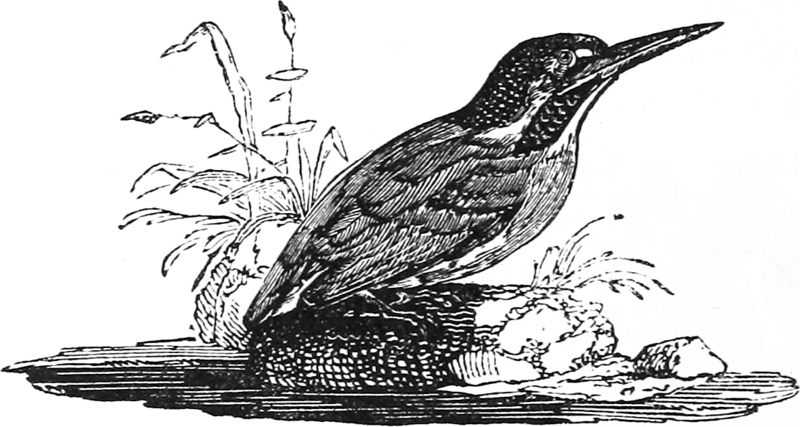
\includegraphics[scale=0.35]{images/Alycon.png}
        \end{figure}
        \vspace{0.5cm}
        \Huge
        \textbf{\textsc{Matematyka Dyskretna}}
        
        \vspace{0.5cm}
        \Large
        \textsc{Wybrane Dowody}
        
        \normalsize
        
        
        \line(1,0){330}
        
        \vspace{1cm}
        \textit{,,Myślę, że 7 punktów na 20 to nie jest zły wynik''}
        \vspace{1cm}

        \textit{\textsc{Popełnione przez}}\\
        \vspace{5mm}

        \textbf{\textsc{Dziurawy Ponton \\ Załatany Ponton \\ Puchaty Pompon \\ Zatopiony Ponton \\ Tonący Ponton \\ Notnop}}

        \vfill

        Kraków \\
        Anno Domini 2023
        
    \end{center}
    
\end{titlepage}


\tableofcontents
\section*{Licencja}
    \begin{figure}[h]
    	\begin{minipage}[c]{0.25\textwidth}
    		
\includegraphics[width=0.7\textwidth]{images/licencja.png}
    	\end{minipage}\hfill
    	\begin{minipage}[c]{0.75\textwidth}
    		\caption*{
    			Ten utwór jest dostępny na 
    			\href{https://creativecommons.org/licenses/by-sa/4.0/}{licencji Creative Commons Uznanie autorstwa
    			na tych samych warunkach 4.0 Międzynarodowe.}
    		}
    	\end{minipage}
    \end{figure}

% Actual content
\mainmatter

\chapter{Kombinatoryka}
 % Żeby nie było syfu to kolejne sekcje dodajemy do chapters/
% A potem includujemy za pomocą \input{chapters/...}

% Używamy \( \) i \[ \] zamiast dolarów -- tak jak się robi w LaTeXu


\documentclass[12pt, a4paper, polish, openany]{book}

% Please, let's familiarize ourselves with notatki.sty and tcs.sty so that we don't reinvent the wheel
\usepackage{notatki}

\fancyhead[L]{\textbf{\textit{MD}}}
\author{
}
\title{TCS and shitposting}


\begin{document}

% Front page and table of contents
\frontmatter

\input{titlepage}

\tableofcontents
\input{license}

% Actual content
\mainmatter

\chapter{Kombinatoryka}
\input{chapters/combinatorics/main}

\chapter{Zasada włączeń i wyłączeń}
\input{chapters/exclusion-inclusion/main}

\chapter{Posety}
\input{chapters/posets/main}

\chapter{Twierdzenie Ramseya}
\input{chapters/ramsey/main}

\chapter{Funkcje tworzące}
\input{chapters/generating_functions/main}

\chapter{Przepływy}
\input{chapters/flows/main}

\chapter{Skojarzenia}
\input{chapters/matchings/main}

\chapter{Kolorowanie grafów}
\input{chapters/graph-coloring/main}

\chapter{Grafy, ale nie kolorowanie}
\input{chapters/graph-misc/main}

\end{document}

\chapter{Zasada włączeń i wyłączeń}
 % Żeby nie było syfu to kolejne sekcje dodajemy do chapters/
% A potem includujemy za pomocą \input{chapters/...}

% Używamy \( \) i \[ \] zamiast dolarów -- tak jak się robi w LaTeXu


\documentclass[12pt, a4paper, polish, openany]{book}

% Please, let's familiarize ourselves with notatki.sty and tcs.sty so that we don't reinvent the wheel
\usepackage{notatki}

\fancyhead[L]{\textbf{\textit{MD}}}
\author{
}
\title{TCS and shitposting}


\begin{document}

% Front page and table of contents
\frontmatter

\input{titlepage}

\tableofcontents
\input{license}

% Actual content
\mainmatter

\chapter{Kombinatoryka}
\input{chapters/combinatorics/main}

\chapter{Zasada włączeń i wyłączeń}
\input{chapters/exclusion-inclusion/main}

\chapter{Posety}
\input{chapters/posets/main}

\chapter{Twierdzenie Ramseya}
\input{chapters/ramsey/main}

\chapter{Funkcje tworzące}
\input{chapters/generating_functions/main}

\chapter{Przepływy}
\input{chapters/flows/main}

\chapter{Skojarzenia}
\input{chapters/matchings/main}

\chapter{Kolorowanie grafów}
\input{chapters/graph-coloring/main}

\chapter{Grafy, ale nie kolorowanie}
\input{chapters/graph-misc/main}

\end{document}

\chapter{Posety}
 % Żeby nie było syfu to kolejne sekcje dodajemy do chapters/
% A potem includujemy za pomocą \input{chapters/...}

% Używamy \( \) i \[ \] zamiast dolarów -- tak jak się robi w LaTeXu


\documentclass[12pt, a4paper, polish, openany]{book}

% Please, let's familiarize ourselves with notatki.sty and tcs.sty so that we don't reinvent the wheel
\usepackage{notatki}

\fancyhead[L]{\textbf{\textit{MD}}}
\author{
}
\title{TCS and shitposting}


\begin{document}

% Front page and table of contents
\frontmatter

\input{titlepage}

\tableofcontents
\input{license}

% Actual content
\mainmatter

\chapter{Kombinatoryka}
\input{chapters/combinatorics/main}

\chapter{Zasada włączeń i wyłączeń}
\input{chapters/exclusion-inclusion/main}

\chapter{Posety}
\input{chapters/posets/main}

\chapter{Twierdzenie Ramseya}
\input{chapters/ramsey/main}

\chapter{Funkcje tworzące}
\input{chapters/generating_functions/main}

\chapter{Przepływy}
\input{chapters/flows/main}

\chapter{Skojarzenia}
\input{chapters/matchings/main}

\chapter{Kolorowanie grafów}
\input{chapters/graph-coloring/main}

\chapter{Grafy, ale nie kolorowanie}
\input{chapters/graph-misc/main}

\end{document}

\chapter{Twierdzenie Ramseya}
 % Żeby nie było syfu to kolejne sekcje dodajemy do chapters/
% A potem includujemy za pomocą \input{chapters/...}

% Używamy \( \) i \[ \] zamiast dolarów -- tak jak się robi w LaTeXu


\documentclass[12pt, a4paper, polish, openany]{book}

% Please, let's familiarize ourselves with notatki.sty and tcs.sty so that we don't reinvent the wheel
\usepackage{notatki}

\fancyhead[L]{\textbf{\textit{MD}}}
\author{
}
\title{TCS and shitposting}


\begin{document}

% Front page and table of contents
\frontmatter

\input{titlepage}

\tableofcontents
\input{license}

% Actual content
\mainmatter

\chapter{Kombinatoryka}
\input{chapters/combinatorics/main}

\chapter{Zasada włączeń i wyłączeń}
\input{chapters/exclusion-inclusion/main}

\chapter{Posety}
\input{chapters/posets/main}

\chapter{Twierdzenie Ramseya}
\input{chapters/ramsey/main}

\chapter{Funkcje tworzące}
\input{chapters/generating_functions/main}

\chapter{Przepływy}
\input{chapters/flows/main}

\chapter{Skojarzenia}
\input{chapters/matchings/main}

\chapter{Kolorowanie grafów}
\input{chapters/graph-coloring/main}

\chapter{Grafy, ale nie kolorowanie}
\input{chapters/graph-misc/main}

\end{document}

\chapter{Funkcje tworzące}
 % Żeby nie było syfu to kolejne sekcje dodajemy do chapters/
% A potem includujemy za pomocą \input{chapters/...}

% Używamy \( \) i \[ \] zamiast dolarów -- tak jak się robi w LaTeXu


\documentclass[12pt, a4paper, polish, openany]{book}

% Please, let's familiarize ourselves with notatki.sty and tcs.sty so that we don't reinvent the wheel
\usepackage{notatki}

\fancyhead[L]{\textbf{\textit{MD}}}
\author{
}
\title{TCS and shitposting}


\begin{document}

% Front page and table of contents
\frontmatter

\input{titlepage}

\tableofcontents
\input{license}

% Actual content
\mainmatter

\chapter{Kombinatoryka}
\input{chapters/combinatorics/main}

\chapter{Zasada włączeń i wyłączeń}
\input{chapters/exclusion-inclusion/main}

\chapter{Posety}
\input{chapters/posets/main}

\chapter{Twierdzenie Ramseya}
\input{chapters/ramsey/main}

\chapter{Funkcje tworzące}
\input{chapters/generating_functions/main}

\chapter{Przepływy}
\input{chapters/flows/main}

\chapter{Skojarzenia}
\input{chapters/matchings/main}

\chapter{Kolorowanie grafów}
\input{chapters/graph-coloring/main}

\chapter{Grafy, ale nie kolorowanie}
\input{chapters/graph-misc/main}

\end{document}

\chapter{Przepływy}
 % Żeby nie było syfu to kolejne sekcje dodajemy do chapters/
% A potem includujemy za pomocą \input{chapters/...}

% Używamy \( \) i \[ \] zamiast dolarów -- tak jak się robi w LaTeXu


\documentclass[12pt, a4paper, polish, openany]{book}

% Please, let's familiarize ourselves with notatki.sty and tcs.sty so that we don't reinvent the wheel
\usepackage{notatki}

\fancyhead[L]{\textbf{\textit{MD}}}
\author{
}
\title{TCS and shitposting}


\begin{document}

% Front page and table of contents
\frontmatter

\input{titlepage}

\tableofcontents
\input{license}

% Actual content
\mainmatter

\chapter{Kombinatoryka}
\input{chapters/combinatorics/main}

\chapter{Zasada włączeń i wyłączeń}
\input{chapters/exclusion-inclusion/main}

\chapter{Posety}
\input{chapters/posets/main}

\chapter{Twierdzenie Ramseya}
\input{chapters/ramsey/main}

\chapter{Funkcje tworzące}
\input{chapters/generating_functions/main}

\chapter{Przepływy}
\input{chapters/flows/main}

\chapter{Skojarzenia}
\input{chapters/matchings/main}

\chapter{Kolorowanie grafów}
\input{chapters/graph-coloring/main}

\chapter{Grafy, ale nie kolorowanie}
\input{chapters/graph-misc/main}

\end{document}

\chapter{Skojarzenia}
 % Żeby nie było syfu to kolejne sekcje dodajemy do chapters/
% A potem includujemy za pomocą \input{chapters/...}

% Używamy \( \) i \[ \] zamiast dolarów -- tak jak się robi w LaTeXu


\documentclass[12pt, a4paper, polish, openany]{book}

% Please, let's familiarize ourselves with notatki.sty and tcs.sty so that we don't reinvent the wheel
\usepackage{notatki}

\fancyhead[L]{\textbf{\textit{MD}}}
\author{
}
\title{TCS and shitposting}


\begin{document}

% Front page and table of contents
\frontmatter

\input{titlepage}

\tableofcontents
\input{license}

% Actual content
\mainmatter

\chapter{Kombinatoryka}
\input{chapters/combinatorics/main}

\chapter{Zasada włączeń i wyłączeń}
\input{chapters/exclusion-inclusion/main}

\chapter{Posety}
\input{chapters/posets/main}

\chapter{Twierdzenie Ramseya}
\input{chapters/ramsey/main}

\chapter{Funkcje tworzące}
\input{chapters/generating_functions/main}

\chapter{Przepływy}
\input{chapters/flows/main}

\chapter{Skojarzenia}
\input{chapters/matchings/main}

\chapter{Kolorowanie grafów}
\input{chapters/graph-coloring/main}

\chapter{Grafy, ale nie kolorowanie}
\input{chapters/graph-misc/main}

\end{document}

\chapter{Kolorowanie grafów}
 % Żeby nie było syfu to kolejne sekcje dodajemy do chapters/
% A potem includujemy za pomocą \input{chapters/...}

% Używamy \( \) i \[ \] zamiast dolarów -- tak jak się robi w LaTeXu


\documentclass[12pt, a4paper, polish, openany]{book}

% Please, let's familiarize ourselves with notatki.sty and tcs.sty so that we don't reinvent the wheel
\usepackage{notatki}

\fancyhead[L]{\textbf{\textit{MD}}}
\author{
}
\title{TCS and shitposting}


\begin{document}

% Front page and table of contents
\frontmatter

\input{titlepage}

\tableofcontents
\input{license}

% Actual content
\mainmatter

\chapter{Kombinatoryka}
\input{chapters/combinatorics/main}

\chapter{Zasada włączeń i wyłączeń}
\input{chapters/exclusion-inclusion/main}

\chapter{Posety}
\input{chapters/posets/main}

\chapter{Twierdzenie Ramseya}
\input{chapters/ramsey/main}

\chapter{Funkcje tworzące}
\input{chapters/generating_functions/main}

\chapter{Przepływy}
\input{chapters/flows/main}

\chapter{Skojarzenia}
\input{chapters/matchings/main}

\chapter{Kolorowanie grafów}
\input{chapters/graph-coloring/main}

\chapter{Grafy, ale nie kolorowanie}
\input{chapters/graph-misc/main}

\end{document}

\chapter{Grafy, ale nie kolorowanie}
 % Żeby nie było syfu to kolejne sekcje dodajemy do chapters/
% A potem includujemy za pomocą \input{chapters/...}

% Używamy \( \) i \[ \] zamiast dolarów -- tak jak się robi w LaTeXu


\documentclass[12pt, a4paper, polish, openany]{book}

% Please, let's familiarize ourselves with notatki.sty and tcs.sty so that we don't reinvent the wheel
\usepackage{notatki}

\fancyhead[L]{\textbf{\textit{MD}}}
\author{
}
\title{TCS and shitposting}


\begin{document}

% Front page and table of contents
\frontmatter

\input{titlepage}

\tableofcontents
\input{license}

% Actual content
\mainmatter

\chapter{Kombinatoryka}
\input{chapters/combinatorics/main}

\chapter{Zasada włączeń i wyłączeń}
\input{chapters/exclusion-inclusion/main}

\chapter{Posety}
\input{chapters/posets/main}

\chapter{Twierdzenie Ramseya}
\input{chapters/ramsey/main}

\chapter{Funkcje tworzące}
\input{chapters/generating_functions/main}

\chapter{Przepływy}
\input{chapters/flows/main}

\chapter{Skojarzenia}
\input{chapters/matchings/main}

\chapter{Kolorowanie grafów}
\input{chapters/graph-coloring/main}

\chapter{Grafy, ale nie kolorowanie}
\input{chapters/graph-misc/main}

\end{document}

\end{document}

\end{document}

\section{Technika zamiatania w geometrii obliczeniowej, zastosowanie do znajdowania wszystkich przecięć odcinków.}
%  % Żeby nie było syfu to kolejne sekcje dodajemy do chapters/
% A potem includujemy za pomocą \input{chapters/...}

% Używamy \( \) i \[ \] zamiast dolarów -- tak jak się robi w LaTeXu


\documentclass[12pt, a4paper, polish, openany]{book}

% Please, let's familiarize ourselves with notatki.sty and tcs.sty so that we don't reinvent the wheel
\usepackage{notatki}

\fancyhead[L]{\textbf{\textit{MD}}}
\author{
}
\title{TCS and shitposting}


\begin{document}

% Front page and table of contents
\frontmatter

\begin{titlepage} 

    \begin{center}
         \begin{figure}[h]
            \centering
            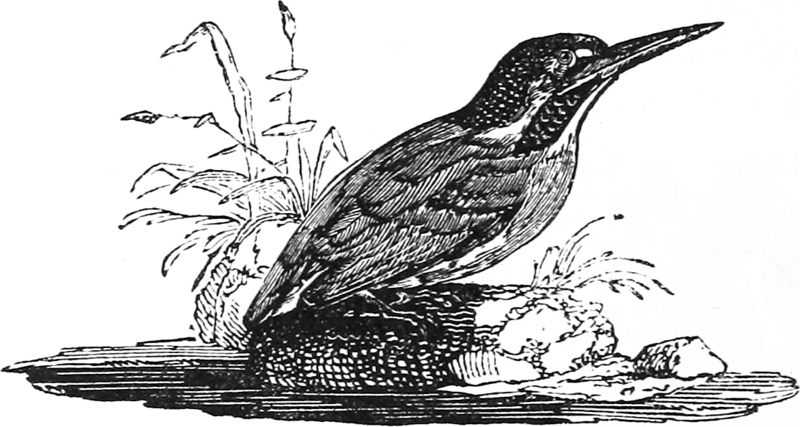
\includegraphics[scale=0.35]{images/Alycon.png}
        \end{figure}
        \vspace{0.5cm}
        \Huge
        \textbf{\textsc{Matematyka Dyskretna}}
        
        \vspace{0.5cm}
        \Large
        \textsc{Wybrane Dowody}
        
        \normalsize
        
        
        \line(1,0){330}
        
        \vspace{1cm}
        \textit{,,Myślę, że 7 punktów na 20 to nie jest zły wynik''}
        \vspace{1cm}

        \textit{\textsc{Popełnione przez}}\\
        \vspace{5mm}

        \textbf{\textsc{Dziurawy Ponton \\ Załatany Ponton \\ Puchaty Pompon \\ Zatopiony Ponton \\ Tonący Ponton \\ Notnop}}

        \vfill

        Kraków \\
        Anno Domini 2023
        
    \end{center}
    
\end{titlepage}


\tableofcontents
\section*{Licencja}
    \begin{figure}[h]
    	\begin{minipage}[c]{0.25\textwidth}
    		
\includegraphics[width=0.7\textwidth]{images/licencja.png}
    	\end{minipage}\hfill
    	\begin{minipage}[c]{0.75\textwidth}
    		\caption*{
    			Ten utwór jest dostępny na 
    			\href{https://creativecommons.org/licenses/by-sa/4.0/}{licencji Creative Commons Uznanie autorstwa
    			na tych samych warunkach 4.0 Międzynarodowe.}
    		}
    	\end{minipage}
    \end{figure}

% Actual content
\mainmatter

\chapter{Kombinatoryka}
 % Żeby nie było syfu to kolejne sekcje dodajemy do chapters/
% A potem includujemy za pomocą \input{chapters/...}

% Używamy \( \) i \[ \] zamiast dolarów -- tak jak się robi w LaTeXu


\documentclass[12pt, a4paper, polish, openany]{book}

% Please, let's familiarize ourselves with notatki.sty and tcs.sty so that we don't reinvent the wheel
\usepackage{notatki}

\fancyhead[L]{\textbf{\textit{MD}}}
\author{
}
\title{TCS and shitposting}


\begin{document}

% Front page and table of contents
\frontmatter

\begin{titlepage} 

    \begin{center}
         \begin{figure}[h]
            \centering
            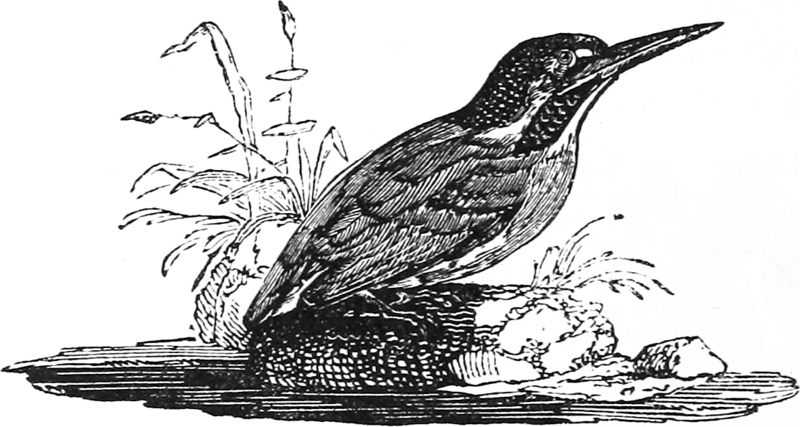
\includegraphics[scale=0.35]{images/Alycon.png}
        \end{figure}
        \vspace{0.5cm}
        \Huge
        \textbf{\textsc{Matematyka Dyskretna}}
        
        \vspace{0.5cm}
        \Large
        \textsc{Wybrane Dowody}
        
        \normalsize
        
        
        \line(1,0){330}
        
        \vspace{1cm}
        \textit{,,Myślę, że 7 punktów na 20 to nie jest zły wynik''}
        \vspace{1cm}

        \textit{\textsc{Popełnione przez}}\\
        \vspace{5mm}

        \textbf{\textsc{Dziurawy Ponton \\ Załatany Ponton \\ Puchaty Pompon \\ Zatopiony Ponton \\ Tonący Ponton \\ Notnop}}

        \vfill

        Kraków \\
        Anno Domini 2023
        
    \end{center}
    
\end{titlepage}


\tableofcontents
\section*{Licencja}
    \begin{figure}[h]
    	\begin{minipage}[c]{0.25\textwidth}
    		
\includegraphics[width=0.7\textwidth]{images/licencja.png}
    	\end{minipage}\hfill
    	\begin{minipage}[c]{0.75\textwidth}
    		\caption*{
    			Ten utwór jest dostępny na 
    			\href{https://creativecommons.org/licenses/by-sa/4.0/}{licencji Creative Commons Uznanie autorstwa
    			na tych samych warunkach 4.0 Międzynarodowe.}
    		}
    	\end{minipage}
    \end{figure}

% Actual content
\mainmatter

\chapter{Kombinatoryka}
 % Żeby nie było syfu to kolejne sekcje dodajemy do chapters/
% A potem includujemy za pomocą \input{chapters/...}

% Używamy \( \) i \[ \] zamiast dolarów -- tak jak się robi w LaTeXu


\documentclass[12pt, a4paper, polish, openany]{book}

% Please, let's familiarize ourselves with notatki.sty and tcs.sty so that we don't reinvent the wheel
\usepackage{notatki}

\fancyhead[L]{\textbf{\textit{MD}}}
\author{
}
\title{TCS and shitposting}


\begin{document}

% Front page and table of contents
\frontmatter

\input{titlepage}

\tableofcontents
\input{license}

% Actual content
\mainmatter

\chapter{Kombinatoryka}
\input{chapters/combinatorics/main}

\chapter{Zasada włączeń i wyłączeń}
\input{chapters/exclusion-inclusion/main}

\chapter{Posety}
\input{chapters/posets/main}

\chapter{Twierdzenie Ramseya}
\input{chapters/ramsey/main}

\chapter{Funkcje tworzące}
\input{chapters/generating_functions/main}

\chapter{Przepływy}
\input{chapters/flows/main}

\chapter{Skojarzenia}
\input{chapters/matchings/main}

\chapter{Kolorowanie grafów}
\input{chapters/graph-coloring/main}

\chapter{Grafy, ale nie kolorowanie}
\input{chapters/graph-misc/main}

\end{document}

\chapter{Zasada włączeń i wyłączeń}
 % Żeby nie było syfu to kolejne sekcje dodajemy do chapters/
% A potem includujemy za pomocą \input{chapters/...}

% Używamy \( \) i \[ \] zamiast dolarów -- tak jak się robi w LaTeXu


\documentclass[12pt, a4paper, polish, openany]{book}

% Please, let's familiarize ourselves with notatki.sty and tcs.sty so that we don't reinvent the wheel
\usepackage{notatki}

\fancyhead[L]{\textbf{\textit{MD}}}
\author{
}
\title{TCS and shitposting}


\begin{document}

% Front page and table of contents
\frontmatter

\input{titlepage}

\tableofcontents
\input{license}

% Actual content
\mainmatter

\chapter{Kombinatoryka}
\input{chapters/combinatorics/main}

\chapter{Zasada włączeń i wyłączeń}
\input{chapters/exclusion-inclusion/main}

\chapter{Posety}
\input{chapters/posets/main}

\chapter{Twierdzenie Ramseya}
\input{chapters/ramsey/main}

\chapter{Funkcje tworzące}
\input{chapters/generating_functions/main}

\chapter{Przepływy}
\input{chapters/flows/main}

\chapter{Skojarzenia}
\input{chapters/matchings/main}

\chapter{Kolorowanie grafów}
\input{chapters/graph-coloring/main}

\chapter{Grafy, ale nie kolorowanie}
\input{chapters/graph-misc/main}

\end{document}

\chapter{Posety}
 % Żeby nie było syfu to kolejne sekcje dodajemy do chapters/
% A potem includujemy za pomocą \input{chapters/...}

% Używamy \( \) i \[ \] zamiast dolarów -- tak jak się robi w LaTeXu


\documentclass[12pt, a4paper, polish, openany]{book}

% Please, let's familiarize ourselves with notatki.sty and tcs.sty so that we don't reinvent the wheel
\usepackage{notatki}

\fancyhead[L]{\textbf{\textit{MD}}}
\author{
}
\title{TCS and shitposting}


\begin{document}

% Front page and table of contents
\frontmatter

\input{titlepage}

\tableofcontents
\input{license}

% Actual content
\mainmatter

\chapter{Kombinatoryka}
\input{chapters/combinatorics/main}

\chapter{Zasada włączeń i wyłączeń}
\input{chapters/exclusion-inclusion/main}

\chapter{Posety}
\input{chapters/posets/main}

\chapter{Twierdzenie Ramseya}
\input{chapters/ramsey/main}

\chapter{Funkcje tworzące}
\input{chapters/generating_functions/main}

\chapter{Przepływy}
\input{chapters/flows/main}

\chapter{Skojarzenia}
\input{chapters/matchings/main}

\chapter{Kolorowanie grafów}
\input{chapters/graph-coloring/main}

\chapter{Grafy, ale nie kolorowanie}
\input{chapters/graph-misc/main}

\end{document}

\chapter{Twierdzenie Ramseya}
 % Żeby nie było syfu to kolejne sekcje dodajemy do chapters/
% A potem includujemy za pomocą \input{chapters/...}

% Używamy \( \) i \[ \] zamiast dolarów -- tak jak się robi w LaTeXu


\documentclass[12pt, a4paper, polish, openany]{book}

% Please, let's familiarize ourselves with notatki.sty and tcs.sty so that we don't reinvent the wheel
\usepackage{notatki}

\fancyhead[L]{\textbf{\textit{MD}}}
\author{
}
\title{TCS and shitposting}


\begin{document}

% Front page and table of contents
\frontmatter

\input{titlepage}

\tableofcontents
\input{license}

% Actual content
\mainmatter

\chapter{Kombinatoryka}
\input{chapters/combinatorics/main}

\chapter{Zasada włączeń i wyłączeń}
\input{chapters/exclusion-inclusion/main}

\chapter{Posety}
\input{chapters/posets/main}

\chapter{Twierdzenie Ramseya}
\input{chapters/ramsey/main}

\chapter{Funkcje tworzące}
\input{chapters/generating_functions/main}

\chapter{Przepływy}
\input{chapters/flows/main}

\chapter{Skojarzenia}
\input{chapters/matchings/main}

\chapter{Kolorowanie grafów}
\input{chapters/graph-coloring/main}

\chapter{Grafy, ale nie kolorowanie}
\input{chapters/graph-misc/main}

\end{document}

\chapter{Funkcje tworzące}
 % Żeby nie było syfu to kolejne sekcje dodajemy do chapters/
% A potem includujemy za pomocą \input{chapters/...}

% Używamy \( \) i \[ \] zamiast dolarów -- tak jak się robi w LaTeXu


\documentclass[12pt, a4paper, polish, openany]{book}

% Please, let's familiarize ourselves with notatki.sty and tcs.sty so that we don't reinvent the wheel
\usepackage{notatki}

\fancyhead[L]{\textbf{\textit{MD}}}
\author{
}
\title{TCS and shitposting}


\begin{document}

% Front page and table of contents
\frontmatter

\input{titlepage}

\tableofcontents
\input{license}

% Actual content
\mainmatter

\chapter{Kombinatoryka}
\input{chapters/combinatorics/main}

\chapter{Zasada włączeń i wyłączeń}
\input{chapters/exclusion-inclusion/main}

\chapter{Posety}
\input{chapters/posets/main}

\chapter{Twierdzenie Ramseya}
\input{chapters/ramsey/main}

\chapter{Funkcje tworzące}
\input{chapters/generating_functions/main}

\chapter{Przepływy}
\input{chapters/flows/main}

\chapter{Skojarzenia}
\input{chapters/matchings/main}

\chapter{Kolorowanie grafów}
\input{chapters/graph-coloring/main}

\chapter{Grafy, ale nie kolorowanie}
\input{chapters/graph-misc/main}

\end{document}

\chapter{Przepływy}
 % Żeby nie było syfu to kolejne sekcje dodajemy do chapters/
% A potem includujemy za pomocą \input{chapters/...}

% Używamy \( \) i \[ \] zamiast dolarów -- tak jak się robi w LaTeXu


\documentclass[12pt, a4paper, polish, openany]{book}

% Please, let's familiarize ourselves with notatki.sty and tcs.sty so that we don't reinvent the wheel
\usepackage{notatki}

\fancyhead[L]{\textbf{\textit{MD}}}
\author{
}
\title{TCS and shitposting}


\begin{document}

% Front page and table of contents
\frontmatter

\input{titlepage}

\tableofcontents
\input{license}

% Actual content
\mainmatter

\chapter{Kombinatoryka}
\input{chapters/combinatorics/main}

\chapter{Zasada włączeń i wyłączeń}
\input{chapters/exclusion-inclusion/main}

\chapter{Posety}
\input{chapters/posets/main}

\chapter{Twierdzenie Ramseya}
\input{chapters/ramsey/main}

\chapter{Funkcje tworzące}
\input{chapters/generating_functions/main}

\chapter{Przepływy}
\input{chapters/flows/main}

\chapter{Skojarzenia}
\input{chapters/matchings/main}

\chapter{Kolorowanie grafów}
\input{chapters/graph-coloring/main}

\chapter{Grafy, ale nie kolorowanie}
\input{chapters/graph-misc/main}

\end{document}

\chapter{Skojarzenia}
 % Żeby nie było syfu to kolejne sekcje dodajemy do chapters/
% A potem includujemy za pomocą \input{chapters/...}

% Używamy \( \) i \[ \] zamiast dolarów -- tak jak się robi w LaTeXu


\documentclass[12pt, a4paper, polish, openany]{book}

% Please, let's familiarize ourselves with notatki.sty and tcs.sty so that we don't reinvent the wheel
\usepackage{notatki}

\fancyhead[L]{\textbf{\textit{MD}}}
\author{
}
\title{TCS and shitposting}


\begin{document}

% Front page and table of contents
\frontmatter

\input{titlepage}

\tableofcontents
\input{license}

% Actual content
\mainmatter

\chapter{Kombinatoryka}
\input{chapters/combinatorics/main}

\chapter{Zasada włączeń i wyłączeń}
\input{chapters/exclusion-inclusion/main}

\chapter{Posety}
\input{chapters/posets/main}

\chapter{Twierdzenie Ramseya}
\input{chapters/ramsey/main}

\chapter{Funkcje tworzące}
\input{chapters/generating_functions/main}

\chapter{Przepływy}
\input{chapters/flows/main}

\chapter{Skojarzenia}
\input{chapters/matchings/main}

\chapter{Kolorowanie grafów}
\input{chapters/graph-coloring/main}

\chapter{Grafy, ale nie kolorowanie}
\input{chapters/graph-misc/main}

\end{document}

\chapter{Kolorowanie grafów}
 % Żeby nie było syfu to kolejne sekcje dodajemy do chapters/
% A potem includujemy za pomocą \input{chapters/...}

% Używamy \( \) i \[ \] zamiast dolarów -- tak jak się robi w LaTeXu


\documentclass[12pt, a4paper, polish, openany]{book}

% Please, let's familiarize ourselves with notatki.sty and tcs.sty so that we don't reinvent the wheel
\usepackage{notatki}

\fancyhead[L]{\textbf{\textit{MD}}}
\author{
}
\title{TCS and shitposting}


\begin{document}

% Front page and table of contents
\frontmatter

\input{titlepage}

\tableofcontents
\input{license}

% Actual content
\mainmatter

\chapter{Kombinatoryka}
\input{chapters/combinatorics/main}

\chapter{Zasada włączeń i wyłączeń}
\input{chapters/exclusion-inclusion/main}

\chapter{Posety}
\input{chapters/posets/main}

\chapter{Twierdzenie Ramseya}
\input{chapters/ramsey/main}

\chapter{Funkcje tworzące}
\input{chapters/generating_functions/main}

\chapter{Przepływy}
\input{chapters/flows/main}

\chapter{Skojarzenia}
\input{chapters/matchings/main}

\chapter{Kolorowanie grafów}
\input{chapters/graph-coloring/main}

\chapter{Grafy, ale nie kolorowanie}
\input{chapters/graph-misc/main}

\end{document}

\chapter{Grafy, ale nie kolorowanie}
 % Żeby nie było syfu to kolejne sekcje dodajemy do chapters/
% A potem includujemy za pomocą \input{chapters/...}

% Używamy \( \) i \[ \] zamiast dolarów -- tak jak się robi w LaTeXu


\documentclass[12pt, a4paper, polish, openany]{book}

% Please, let's familiarize ourselves with notatki.sty and tcs.sty so that we don't reinvent the wheel
\usepackage{notatki}

\fancyhead[L]{\textbf{\textit{MD}}}
\author{
}
\title{TCS and shitposting}


\begin{document}

% Front page and table of contents
\frontmatter

\input{titlepage}

\tableofcontents
\input{license}

% Actual content
\mainmatter

\chapter{Kombinatoryka}
\input{chapters/combinatorics/main}

\chapter{Zasada włączeń i wyłączeń}
\input{chapters/exclusion-inclusion/main}

\chapter{Posety}
\input{chapters/posets/main}

\chapter{Twierdzenie Ramseya}
\input{chapters/ramsey/main}

\chapter{Funkcje tworzące}
\input{chapters/generating_functions/main}

\chapter{Przepływy}
\input{chapters/flows/main}

\chapter{Skojarzenia}
\input{chapters/matchings/main}

\chapter{Kolorowanie grafów}
\input{chapters/graph-coloring/main}

\chapter{Grafy, ale nie kolorowanie}
\input{chapters/graph-misc/main}

\end{document}

\end{document}

\chapter{Zasada włączeń i wyłączeń}
 % Żeby nie było syfu to kolejne sekcje dodajemy do chapters/
% A potem includujemy za pomocą \input{chapters/...}

% Używamy \( \) i \[ \] zamiast dolarów -- tak jak się robi w LaTeXu


\documentclass[12pt, a4paper, polish, openany]{book}

% Please, let's familiarize ourselves with notatki.sty and tcs.sty so that we don't reinvent the wheel
\usepackage{notatki}

\fancyhead[L]{\textbf{\textit{MD}}}
\author{
}
\title{TCS and shitposting}


\begin{document}

% Front page and table of contents
\frontmatter

\begin{titlepage} 

    \begin{center}
         \begin{figure}[h]
            \centering
            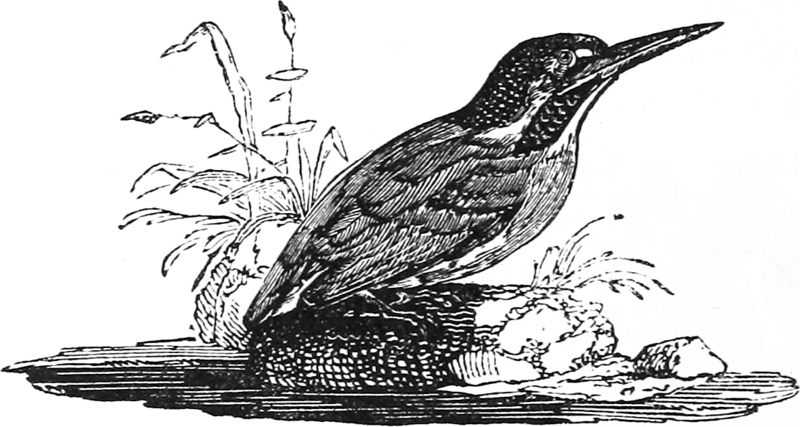
\includegraphics[scale=0.35]{images/Alycon.png}
        \end{figure}
        \vspace{0.5cm}
        \Huge
        \textbf{\textsc{Matematyka Dyskretna}}
        
        \vspace{0.5cm}
        \Large
        \textsc{Wybrane Dowody}
        
        \normalsize
        
        
        \line(1,0){330}
        
        \vspace{1cm}
        \textit{,,Myślę, że 7 punktów na 20 to nie jest zły wynik''}
        \vspace{1cm}

        \textit{\textsc{Popełnione przez}}\\
        \vspace{5mm}

        \textbf{\textsc{Dziurawy Ponton \\ Załatany Ponton \\ Puchaty Pompon \\ Zatopiony Ponton \\ Tonący Ponton \\ Notnop}}

        \vfill

        Kraków \\
        Anno Domini 2023
        
    \end{center}
    
\end{titlepage}


\tableofcontents
\section*{Licencja}
    \begin{figure}[h]
    	\begin{minipage}[c]{0.25\textwidth}
    		
\includegraphics[width=0.7\textwidth]{images/licencja.png}
    	\end{minipage}\hfill
    	\begin{minipage}[c]{0.75\textwidth}
    		\caption*{
    			Ten utwór jest dostępny na 
    			\href{https://creativecommons.org/licenses/by-sa/4.0/}{licencji Creative Commons Uznanie autorstwa
    			na tych samych warunkach 4.0 Międzynarodowe.}
    		}
    	\end{minipage}
    \end{figure}

% Actual content
\mainmatter

\chapter{Kombinatoryka}
 % Żeby nie było syfu to kolejne sekcje dodajemy do chapters/
% A potem includujemy za pomocą \input{chapters/...}

% Używamy \( \) i \[ \] zamiast dolarów -- tak jak się robi w LaTeXu


\documentclass[12pt, a4paper, polish, openany]{book}

% Please, let's familiarize ourselves with notatki.sty and tcs.sty so that we don't reinvent the wheel
\usepackage{notatki}

\fancyhead[L]{\textbf{\textit{MD}}}
\author{
}
\title{TCS and shitposting}


\begin{document}

% Front page and table of contents
\frontmatter

\input{titlepage}

\tableofcontents
\input{license}

% Actual content
\mainmatter

\chapter{Kombinatoryka}
\input{chapters/combinatorics/main}

\chapter{Zasada włączeń i wyłączeń}
\input{chapters/exclusion-inclusion/main}

\chapter{Posety}
\input{chapters/posets/main}

\chapter{Twierdzenie Ramseya}
\input{chapters/ramsey/main}

\chapter{Funkcje tworzące}
\input{chapters/generating_functions/main}

\chapter{Przepływy}
\input{chapters/flows/main}

\chapter{Skojarzenia}
\input{chapters/matchings/main}

\chapter{Kolorowanie grafów}
\input{chapters/graph-coloring/main}

\chapter{Grafy, ale nie kolorowanie}
\input{chapters/graph-misc/main}

\end{document}

\chapter{Zasada włączeń i wyłączeń}
 % Żeby nie było syfu to kolejne sekcje dodajemy do chapters/
% A potem includujemy za pomocą \input{chapters/...}

% Używamy \( \) i \[ \] zamiast dolarów -- tak jak się robi w LaTeXu


\documentclass[12pt, a4paper, polish, openany]{book}

% Please, let's familiarize ourselves with notatki.sty and tcs.sty so that we don't reinvent the wheel
\usepackage{notatki}

\fancyhead[L]{\textbf{\textit{MD}}}
\author{
}
\title{TCS and shitposting}


\begin{document}

% Front page and table of contents
\frontmatter

\input{titlepage}

\tableofcontents
\input{license}

% Actual content
\mainmatter

\chapter{Kombinatoryka}
\input{chapters/combinatorics/main}

\chapter{Zasada włączeń i wyłączeń}
\input{chapters/exclusion-inclusion/main}

\chapter{Posety}
\input{chapters/posets/main}

\chapter{Twierdzenie Ramseya}
\input{chapters/ramsey/main}

\chapter{Funkcje tworzące}
\input{chapters/generating_functions/main}

\chapter{Przepływy}
\input{chapters/flows/main}

\chapter{Skojarzenia}
\input{chapters/matchings/main}

\chapter{Kolorowanie grafów}
\input{chapters/graph-coloring/main}

\chapter{Grafy, ale nie kolorowanie}
\input{chapters/graph-misc/main}

\end{document}

\chapter{Posety}
 % Żeby nie było syfu to kolejne sekcje dodajemy do chapters/
% A potem includujemy za pomocą \input{chapters/...}

% Używamy \( \) i \[ \] zamiast dolarów -- tak jak się robi w LaTeXu


\documentclass[12pt, a4paper, polish, openany]{book}

% Please, let's familiarize ourselves with notatki.sty and tcs.sty so that we don't reinvent the wheel
\usepackage{notatki}

\fancyhead[L]{\textbf{\textit{MD}}}
\author{
}
\title{TCS and shitposting}


\begin{document}

% Front page and table of contents
\frontmatter

\input{titlepage}

\tableofcontents
\input{license}

% Actual content
\mainmatter

\chapter{Kombinatoryka}
\input{chapters/combinatorics/main}

\chapter{Zasada włączeń i wyłączeń}
\input{chapters/exclusion-inclusion/main}

\chapter{Posety}
\input{chapters/posets/main}

\chapter{Twierdzenie Ramseya}
\input{chapters/ramsey/main}

\chapter{Funkcje tworzące}
\input{chapters/generating_functions/main}

\chapter{Przepływy}
\input{chapters/flows/main}

\chapter{Skojarzenia}
\input{chapters/matchings/main}

\chapter{Kolorowanie grafów}
\input{chapters/graph-coloring/main}

\chapter{Grafy, ale nie kolorowanie}
\input{chapters/graph-misc/main}

\end{document}

\chapter{Twierdzenie Ramseya}
 % Żeby nie było syfu to kolejne sekcje dodajemy do chapters/
% A potem includujemy za pomocą \input{chapters/...}

% Używamy \( \) i \[ \] zamiast dolarów -- tak jak się robi w LaTeXu


\documentclass[12pt, a4paper, polish, openany]{book}

% Please, let's familiarize ourselves with notatki.sty and tcs.sty so that we don't reinvent the wheel
\usepackage{notatki}

\fancyhead[L]{\textbf{\textit{MD}}}
\author{
}
\title{TCS and shitposting}


\begin{document}

% Front page and table of contents
\frontmatter

\input{titlepage}

\tableofcontents
\input{license}

% Actual content
\mainmatter

\chapter{Kombinatoryka}
\input{chapters/combinatorics/main}

\chapter{Zasada włączeń i wyłączeń}
\input{chapters/exclusion-inclusion/main}

\chapter{Posety}
\input{chapters/posets/main}

\chapter{Twierdzenie Ramseya}
\input{chapters/ramsey/main}

\chapter{Funkcje tworzące}
\input{chapters/generating_functions/main}

\chapter{Przepływy}
\input{chapters/flows/main}

\chapter{Skojarzenia}
\input{chapters/matchings/main}

\chapter{Kolorowanie grafów}
\input{chapters/graph-coloring/main}

\chapter{Grafy, ale nie kolorowanie}
\input{chapters/graph-misc/main}

\end{document}

\chapter{Funkcje tworzące}
 % Żeby nie było syfu to kolejne sekcje dodajemy do chapters/
% A potem includujemy za pomocą \input{chapters/...}

% Używamy \( \) i \[ \] zamiast dolarów -- tak jak się robi w LaTeXu


\documentclass[12pt, a4paper, polish, openany]{book}

% Please, let's familiarize ourselves with notatki.sty and tcs.sty so that we don't reinvent the wheel
\usepackage{notatki}

\fancyhead[L]{\textbf{\textit{MD}}}
\author{
}
\title{TCS and shitposting}


\begin{document}

% Front page and table of contents
\frontmatter

\input{titlepage}

\tableofcontents
\input{license}

% Actual content
\mainmatter

\chapter{Kombinatoryka}
\input{chapters/combinatorics/main}

\chapter{Zasada włączeń i wyłączeń}
\input{chapters/exclusion-inclusion/main}

\chapter{Posety}
\input{chapters/posets/main}

\chapter{Twierdzenie Ramseya}
\input{chapters/ramsey/main}

\chapter{Funkcje tworzące}
\input{chapters/generating_functions/main}

\chapter{Przepływy}
\input{chapters/flows/main}

\chapter{Skojarzenia}
\input{chapters/matchings/main}

\chapter{Kolorowanie grafów}
\input{chapters/graph-coloring/main}

\chapter{Grafy, ale nie kolorowanie}
\input{chapters/graph-misc/main}

\end{document}

\chapter{Przepływy}
 % Żeby nie było syfu to kolejne sekcje dodajemy do chapters/
% A potem includujemy za pomocą \input{chapters/...}

% Używamy \( \) i \[ \] zamiast dolarów -- tak jak się robi w LaTeXu


\documentclass[12pt, a4paper, polish, openany]{book}

% Please, let's familiarize ourselves with notatki.sty and tcs.sty so that we don't reinvent the wheel
\usepackage{notatki}

\fancyhead[L]{\textbf{\textit{MD}}}
\author{
}
\title{TCS and shitposting}


\begin{document}

% Front page and table of contents
\frontmatter

\input{titlepage}

\tableofcontents
\input{license}

% Actual content
\mainmatter

\chapter{Kombinatoryka}
\input{chapters/combinatorics/main}

\chapter{Zasada włączeń i wyłączeń}
\input{chapters/exclusion-inclusion/main}

\chapter{Posety}
\input{chapters/posets/main}

\chapter{Twierdzenie Ramseya}
\input{chapters/ramsey/main}

\chapter{Funkcje tworzące}
\input{chapters/generating_functions/main}

\chapter{Przepływy}
\input{chapters/flows/main}

\chapter{Skojarzenia}
\input{chapters/matchings/main}

\chapter{Kolorowanie grafów}
\input{chapters/graph-coloring/main}

\chapter{Grafy, ale nie kolorowanie}
\input{chapters/graph-misc/main}

\end{document}

\chapter{Skojarzenia}
 % Żeby nie było syfu to kolejne sekcje dodajemy do chapters/
% A potem includujemy za pomocą \input{chapters/...}

% Używamy \( \) i \[ \] zamiast dolarów -- tak jak się robi w LaTeXu


\documentclass[12pt, a4paper, polish, openany]{book}

% Please, let's familiarize ourselves with notatki.sty and tcs.sty so that we don't reinvent the wheel
\usepackage{notatki}

\fancyhead[L]{\textbf{\textit{MD}}}
\author{
}
\title{TCS and shitposting}


\begin{document}

% Front page and table of contents
\frontmatter

\input{titlepage}

\tableofcontents
\input{license}

% Actual content
\mainmatter

\chapter{Kombinatoryka}
\input{chapters/combinatorics/main}

\chapter{Zasada włączeń i wyłączeń}
\input{chapters/exclusion-inclusion/main}

\chapter{Posety}
\input{chapters/posets/main}

\chapter{Twierdzenie Ramseya}
\input{chapters/ramsey/main}

\chapter{Funkcje tworzące}
\input{chapters/generating_functions/main}

\chapter{Przepływy}
\input{chapters/flows/main}

\chapter{Skojarzenia}
\input{chapters/matchings/main}

\chapter{Kolorowanie grafów}
\input{chapters/graph-coloring/main}

\chapter{Grafy, ale nie kolorowanie}
\input{chapters/graph-misc/main}

\end{document}

\chapter{Kolorowanie grafów}
 % Żeby nie było syfu to kolejne sekcje dodajemy do chapters/
% A potem includujemy za pomocą \input{chapters/...}

% Używamy \( \) i \[ \] zamiast dolarów -- tak jak się robi w LaTeXu


\documentclass[12pt, a4paper, polish, openany]{book}

% Please, let's familiarize ourselves with notatki.sty and tcs.sty so that we don't reinvent the wheel
\usepackage{notatki}

\fancyhead[L]{\textbf{\textit{MD}}}
\author{
}
\title{TCS and shitposting}


\begin{document}

% Front page and table of contents
\frontmatter

\input{titlepage}

\tableofcontents
\input{license}

% Actual content
\mainmatter

\chapter{Kombinatoryka}
\input{chapters/combinatorics/main}

\chapter{Zasada włączeń i wyłączeń}
\input{chapters/exclusion-inclusion/main}

\chapter{Posety}
\input{chapters/posets/main}

\chapter{Twierdzenie Ramseya}
\input{chapters/ramsey/main}

\chapter{Funkcje tworzące}
\input{chapters/generating_functions/main}

\chapter{Przepływy}
\input{chapters/flows/main}

\chapter{Skojarzenia}
\input{chapters/matchings/main}

\chapter{Kolorowanie grafów}
\input{chapters/graph-coloring/main}

\chapter{Grafy, ale nie kolorowanie}
\input{chapters/graph-misc/main}

\end{document}

\chapter{Grafy, ale nie kolorowanie}
 % Żeby nie było syfu to kolejne sekcje dodajemy do chapters/
% A potem includujemy za pomocą \input{chapters/...}

% Używamy \( \) i \[ \] zamiast dolarów -- tak jak się robi w LaTeXu


\documentclass[12pt, a4paper, polish, openany]{book}

% Please, let's familiarize ourselves with notatki.sty and tcs.sty so that we don't reinvent the wheel
\usepackage{notatki}

\fancyhead[L]{\textbf{\textit{MD}}}
\author{
}
\title{TCS and shitposting}


\begin{document}

% Front page and table of contents
\frontmatter

\input{titlepage}

\tableofcontents
\input{license}

% Actual content
\mainmatter

\chapter{Kombinatoryka}
\input{chapters/combinatorics/main}

\chapter{Zasada włączeń i wyłączeń}
\input{chapters/exclusion-inclusion/main}

\chapter{Posety}
\input{chapters/posets/main}

\chapter{Twierdzenie Ramseya}
\input{chapters/ramsey/main}

\chapter{Funkcje tworzące}
\input{chapters/generating_functions/main}

\chapter{Przepływy}
\input{chapters/flows/main}

\chapter{Skojarzenia}
\input{chapters/matchings/main}

\chapter{Kolorowanie grafów}
\input{chapters/graph-coloring/main}

\chapter{Grafy, ale nie kolorowanie}
\input{chapters/graph-misc/main}

\end{document}

\end{document}

\chapter{Posety}
 % Żeby nie było syfu to kolejne sekcje dodajemy do chapters/
% A potem includujemy za pomocą \input{chapters/...}

% Używamy \( \) i \[ \] zamiast dolarów -- tak jak się robi w LaTeXu


\documentclass[12pt, a4paper, polish, openany]{book}

% Please, let's familiarize ourselves with notatki.sty and tcs.sty so that we don't reinvent the wheel
\usepackage{notatki}

\fancyhead[L]{\textbf{\textit{MD}}}
\author{
}
\title{TCS and shitposting}


\begin{document}

% Front page and table of contents
\frontmatter

\begin{titlepage} 

    \begin{center}
         \begin{figure}[h]
            \centering
            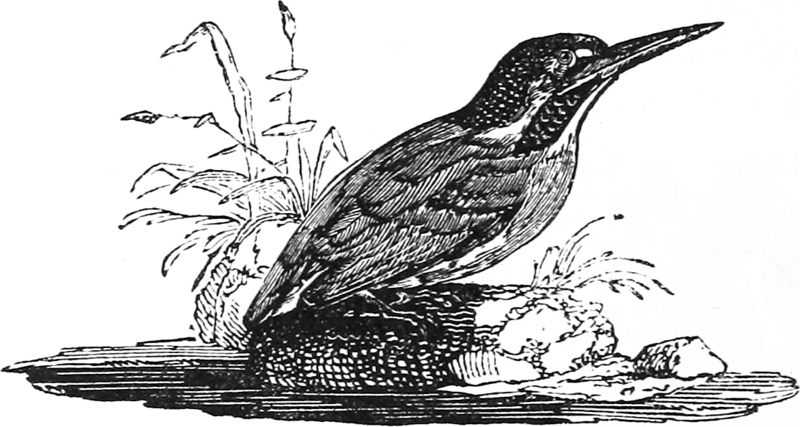
\includegraphics[scale=0.35]{images/Alycon.png}
        \end{figure}
        \vspace{0.5cm}
        \Huge
        \textbf{\textsc{Matematyka Dyskretna}}
        
        \vspace{0.5cm}
        \Large
        \textsc{Wybrane Dowody}
        
        \normalsize
        
        
        \line(1,0){330}
        
        \vspace{1cm}
        \textit{,,Myślę, że 7 punktów na 20 to nie jest zły wynik''}
        \vspace{1cm}

        \textit{\textsc{Popełnione przez}}\\
        \vspace{5mm}

        \textbf{\textsc{Dziurawy Ponton \\ Załatany Ponton \\ Puchaty Pompon \\ Zatopiony Ponton \\ Tonący Ponton \\ Notnop}}

        \vfill

        Kraków \\
        Anno Domini 2023
        
    \end{center}
    
\end{titlepage}


\tableofcontents
\section*{Licencja}
    \begin{figure}[h]
    	\begin{minipage}[c]{0.25\textwidth}
    		
\includegraphics[width=0.7\textwidth]{images/licencja.png}
    	\end{minipage}\hfill
    	\begin{minipage}[c]{0.75\textwidth}
    		\caption*{
    			Ten utwór jest dostępny na 
    			\href{https://creativecommons.org/licenses/by-sa/4.0/}{licencji Creative Commons Uznanie autorstwa
    			na tych samych warunkach 4.0 Międzynarodowe.}
    		}
    	\end{minipage}
    \end{figure}

% Actual content
\mainmatter

\chapter{Kombinatoryka}
 % Żeby nie było syfu to kolejne sekcje dodajemy do chapters/
% A potem includujemy za pomocą \input{chapters/...}

% Używamy \( \) i \[ \] zamiast dolarów -- tak jak się robi w LaTeXu


\documentclass[12pt, a4paper, polish, openany]{book}

% Please, let's familiarize ourselves with notatki.sty and tcs.sty so that we don't reinvent the wheel
\usepackage{notatki}

\fancyhead[L]{\textbf{\textit{MD}}}
\author{
}
\title{TCS and shitposting}


\begin{document}

% Front page and table of contents
\frontmatter

\input{titlepage}

\tableofcontents
\input{license}

% Actual content
\mainmatter

\chapter{Kombinatoryka}
\input{chapters/combinatorics/main}

\chapter{Zasada włączeń i wyłączeń}
\input{chapters/exclusion-inclusion/main}

\chapter{Posety}
\input{chapters/posets/main}

\chapter{Twierdzenie Ramseya}
\input{chapters/ramsey/main}

\chapter{Funkcje tworzące}
\input{chapters/generating_functions/main}

\chapter{Przepływy}
\input{chapters/flows/main}

\chapter{Skojarzenia}
\input{chapters/matchings/main}

\chapter{Kolorowanie grafów}
\input{chapters/graph-coloring/main}

\chapter{Grafy, ale nie kolorowanie}
\input{chapters/graph-misc/main}

\end{document}

\chapter{Zasada włączeń i wyłączeń}
 % Żeby nie było syfu to kolejne sekcje dodajemy do chapters/
% A potem includujemy za pomocą \input{chapters/...}

% Używamy \( \) i \[ \] zamiast dolarów -- tak jak się robi w LaTeXu


\documentclass[12pt, a4paper, polish, openany]{book}

% Please, let's familiarize ourselves with notatki.sty and tcs.sty so that we don't reinvent the wheel
\usepackage{notatki}

\fancyhead[L]{\textbf{\textit{MD}}}
\author{
}
\title{TCS and shitposting}


\begin{document}

% Front page and table of contents
\frontmatter

\input{titlepage}

\tableofcontents
\input{license}

% Actual content
\mainmatter

\chapter{Kombinatoryka}
\input{chapters/combinatorics/main}

\chapter{Zasada włączeń i wyłączeń}
\input{chapters/exclusion-inclusion/main}

\chapter{Posety}
\input{chapters/posets/main}

\chapter{Twierdzenie Ramseya}
\input{chapters/ramsey/main}

\chapter{Funkcje tworzące}
\input{chapters/generating_functions/main}

\chapter{Przepływy}
\input{chapters/flows/main}

\chapter{Skojarzenia}
\input{chapters/matchings/main}

\chapter{Kolorowanie grafów}
\input{chapters/graph-coloring/main}

\chapter{Grafy, ale nie kolorowanie}
\input{chapters/graph-misc/main}

\end{document}

\chapter{Posety}
 % Żeby nie było syfu to kolejne sekcje dodajemy do chapters/
% A potem includujemy za pomocą \input{chapters/...}

% Używamy \( \) i \[ \] zamiast dolarów -- tak jak się robi w LaTeXu


\documentclass[12pt, a4paper, polish, openany]{book}

% Please, let's familiarize ourselves with notatki.sty and tcs.sty so that we don't reinvent the wheel
\usepackage{notatki}

\fancyhead[L]{\textbf{\textit{MD}}}
\author{
}
\title{TCS and shitposting}


\begin{document}

% Front page and table of contents
\frontmatter

\input{titlepage}

\tableofcontents
\input{license}

% Actual content
\mainmatter

\chapter{Kombinatoryka}
\input{chapters/combinatorics/main}

\chapter{Zasada włączeń i wyłączeń}
\input{chapters/exclusion-inclusion/main}

\chapter{Posety}
\input{chapters/posets/main}

\chapter{Twierdzenie Ramseya}
\input{chapters/ramsey/main}

\chapter{Funkcje tworzące}
\input{chapters/generating_functions/main}

\chapter{Przepływy}
\input{chapters/flows/main}

\chapter{Skojarzenia}
\input{chapters/matchings/main}

\chapter{Kolorowanie grafów}
\input{chapters/graph-coloring/main}

\chapter{Grafy, ale nie kolorowanie}
\input{chapters/graph-misc/main}

\end{document}

\chapter{Twierdzenie Ramseya}
 % Żeby nie było syfu to kolejne sekcje dodajemy do chapters/
% A potem includujemy za pomocą \input{chapters/...}

% Używamy \( \) i \[ \] zamiast dolarów -- tak jak się robi w LaTeXu


\documentclass[12pt, a4paper, polish, openany]{book}

% Please, let's familiarize ourselves with notatki.sty and tcs.sty so that we don't reinvent the wheel
\usepackage{notatki}

\fancyhead[L]{\textbf{\textit{MD}}}
\author{
}
\title{TCS and shitposting}


\begin{document}

% Front page and table of contents
\frontmatter

\input{titlepage}

\tableofcontents
\input{license}

% Actual content
\mainmatter

\chapter{Kombinatoryka}
\input{chapters/combinatorics/main}

\chapter{Zasada włączeń i wyłączeń}
\input{chapters/exclusion-inclusion/main}

\chapter{Posety}
\input{chapters/posets/main}

\chapter{Twierdzenie Ramseya}
\input{chapters/ramsey/main}

\chapter{Funkcje tworzące}
\input{chapters/generating_functions/main}

\chapter{Przepływy}
\input{chapters/flows/main}

\chapter{Skojarzenia}
\input{chapters/matchings/main}

\chapter{Kolorowanie grafów}
\input{chapters/graph-coloring/main}

\chapter{Grafy, ale nie kolorowanie}
\input{chapters/graph-misc/main}

\end{document}

\chapter{Funkcje tworzące}
 % Żeby nie było syfu to kolejne sekcje dodajemy do chapters/
% A potem includujemy za pomocą \input{chapters/...}

% Używamy \( \) i \[ \] zamiast dolarów -- tak jak się robi w LaTeXu


\documentclass[12pt, a4paper, polish, openany]{book}

% Please, let's familiarize ourselves with notatki.sty and tcs.sty so that we don't reinvent the wheel
\usepackage{notatki}

\fancyhead[L]{\textbf{\textit{MD}}}
\author{
}
\title{TCS and shitposting}


\begin{document}

% Front page and table of contents
\frontmatter

\input{titlepage}

\tableofcontents
\input{license}

% Actual content
\mainmatter

\chapter{Kombinatoryka}
\input{chapters/combinatorics/main}

\chapter{Zasada włączeń i wyłączeń}
\input{chapters/exclusion-inclusion/main}

\chapter{Posety}
\input{chapters/posets/main}

\chapter{Twierdzenie Ramseya}
\input{chapters/ramsey/main}

\chapter{Funkcje tworzące}
\input{chapters/generating_functions/main}

\chapter{Przepływy}
\input{chapters/flows/main}

\chapter{Skojarzenia}
\input{chapters/matchings/main}

\chapter{Kolorowanie grafów}
\input{chapters/graph-coloring/main}

\chapter{Grafy, ale nie kolorowanie}
\input{chapters/graph-misc/main}

\end{document}

\chapter{Przepływy}
 % Żeby nie było syfu to kolejne sekcje dodajemy do chapters/
% A potem includujemy za pomocą \input{chapters/...}

% Używamy \( \) i \[ \] zamiast dolarów -- tak jak się robi w LaTeXu


\documentclass[12pt, a4paper, polish, openany]{book}

% Please, let's familiarize ourselves with notatki.sty and tcs.sty so that we don't reinvent the wheel
\usepackage{notatki}

\fancyhead[L]{\textbf{\textit{MD}}}
\author{
}
\title{TCS and shitposting}


\begin{document}

% Front page and table of contents
\frontmatter

\input{titlepage}

\tableofcontents
\input{license}

% Actual content
\mainmatter

\chapter{Kombinatoryka}
\input{chapters/combinatorics/main}

\chapter{Zasada włączeń i wyłączeń}
\input{chapters/exclusion-inclusion/main}

\chapter{Posety}
\input{chapters/posets/main}

\chapter{Twierdzenie Ramseya}
\input{chapters/ramsey/main}

\chapter{Funkcje tworzące}
\input{chapters/generating_functions/main}

\chapter{Przepływy}
\input{chapters/flows/main}

\chapter{Skojarzenia}
\input{chapters/matchings/main}

\chapter{Kolorowanie grafów}
\input{chapters/graph-coloring/main}

\chapter{Grafy, ale nie kolorowanie}
\input{chapters/graph-misc/main}

\end{document}

\chapter{Skojarzenia}
 % Żeby nie było syfu to kolejne sekcje dodajemy do chapters/
% A potem includujemy za pomocą \input{chapters/...}

% Używamy \( \) i \[ \] zamiast dolarów -- tak jak się robi w LaTeXu


\documentclass[12pt, a4paper, polish, openany]{book}

% Please, let's familiarize ourselves with notatki.sty and tcs.sty so that we don't reinvent the wheel
\usepackage{notatki}

\fancyhead[L]{\textbf{\textit{MD}}}
\author{
}
\title{TCS and shitposting}


\begin{document}

% Front page and table of contents
\frontmatter

\input{titlepage}

\tableofcontents
\input{license}

% Actual content
\mainmatter

\chapter{Kombinatoryka}
\input{chapters/combinatorics/main}

\chapter{Zasada włączeń i wyłączeń}
\input{chapters/exclusion-inclusion/main}

\chapter{Posety}
\input{chapters/posets/main}

\chapter{Twierdzenie Ramseya}
\input{chapters/ramsey/main}

\chapter{Funkcje tworzące}
\input{chapters/generating_functions/main}

\chapter{Przepływy}
\input{chapters/flows/main}

\chapter{Skojarzenia}
\input{chapters/matchings/main}

\chapter{Kolorowanie grafów}
\input{chapters/graph-coloring/main}

\chapter{Grafy, ale nie kolorowanie}
\input{chapters/graph-misc/main}

\end{document}

\chapter{Kolorowanie grafów}
 % Żeby nie było syfu to kolejne sekcje dodajemy do chapters/
% A potem includujemy za pomocą \input{chapters/...}

% Używamy \( \) i \[ \] zamiast dolarów -- tak jak się robi w LaTeXu


\documentclass[12pt, a4paper, polish, openany]{book}

% Please, let's familiarize ourselves with notatki.sty and tcs.sty so that we don't reinvent the wheel
\usepackage{notatki}

\fancyhead[L]{\textbf{\textit{MD}}}
\author{
}
\title{TCS and shitposting}


\begin{document}

% Front page and table of contents
\frontmatter

\input{titlepage}

\tableofcontents
\input{license}

% Actual content
\mainmatter

\chapter{Kombinatoryka}
\input{chapters/combinatorics/main}

\chapter{Zasada włączeń i wyłączeń}
\input{chapters/exclusion-inclusion/main}

\chapter{Posety}
\input{chapters/posets/main}

\chapter{Twierdzenie Ramseya}
\input{chapters/ramsey/main}

\chapter{Funkcje tworzące}
\input{chapters/generating_functions/main}

\chapter{Przepływy}
\input{chapters/flows/main}

\chapter{Skojarzenia}
\input{chapters/matchings/main}

\chapter{Kolorowanie grafów}
\input{chapters/graph-coloring/main}

\chapter{Grafy, ale nie kolorowanie}
\input{chapters/graph-misc/main}

\end{document}

\chapter{Grafy, ale nie kolorowanie}
 % Żeby nie było syfu to kolejne sekcje dodajemy do chapters/
% A potem includujemy za pomocą \input{chapters/...}

% Używamy \( \) i \[ \] zamiast dolarów -- tak jak się robi w LaTeXu


\documentclass[12pt, a4paper, polish, openany]{book}

% Please, let's familiarize ourselves with notatki.sty and tcs.sty so that we don't reinvent the wheel
\usepackage{notatki}

\fancyhead[L]{\textbf{\textit{MD}}}
\author{
}
\title{TCS and shitposting}


\begin{document}

% Front page and table of contents
\frontmatter

\input{titlepage}

\tableofcontents
\input{license}

% Actual content
\mainmatter

\chapter{Kombinatoryka}
\input{chapters/combinatorics/main}

\chapter{Zasada włączeń i wyłączeń}
\input{chapters/exclusion-inclusion/main}

\chapter{Posety}
\input{chapters/posets/main}

\chapter{Twierdzenie Ramseya}
\input{chapters/ramsey/main}

\chapter{Funkcje tworzące}
\input{chapters/generating_functions/main}

\chapter{Przepływy}
\input{chapters/flows/main}

\chapter{Skojarzenia}
\input{chapters/matchings/main}

\chapter{Kolorowanie grafów}
\input{chapters/graph-coloring/main}

\chapter{Grafy, ale nie kolorowanie}
\input{chapters/graph-misc/main}

\end{document}

\end{document}

\chapter{Twierdzenie Ramseya}
 % Żeby nie było syfu to kolejne sekcje dodajemy do chapters/
% A potem includujemy za pomocą \input{chapters/...}

% Używamy \( \) i \[ \] zamiast dolarów -- tak jak się robi w LaTeXu


\documentclass[12pt, a4paper, polish, openany]{book}

% Please, let's familiarize ourselves with notatki.sty and tcs.sty so that we don't reinvent the wheel
\usepackage{notatki}

\fancyhead[L]{\textbf{\textit{MD}}}
\author{
}
\title{TCS and shitposting}


\begin{document}

% Front page and table of contents
\frontmatter

\begin{titlepage} 

    \begin{center}
         \begin{figure}[h]
            \centering
            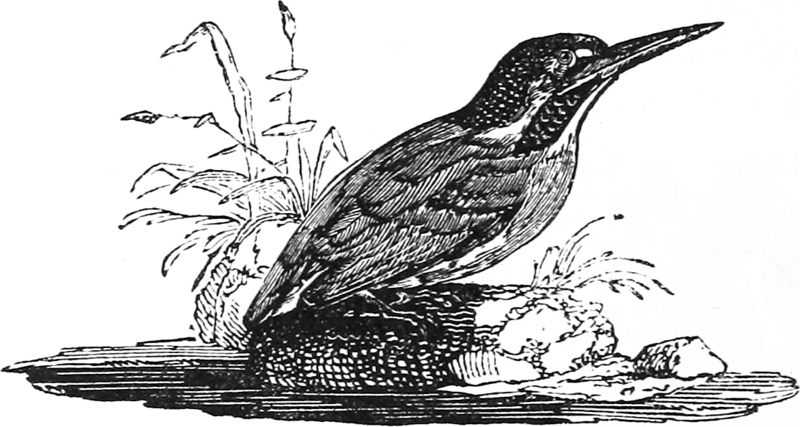
\includegraphics[scale=0.35]{images/Alycon.png}
        \end{figure}
        \vspace{0.5cm}
        \Huge
        \textbf{\textsc{Matematyka Dyskretna}}
        
        \vspace{0.5cm}
        \Large
        \textsc{Wybrane Dowody}
        
        \normalsize
        
        
        \line(1,0){330}
        
        \vspace{1cm}
        \textit{,,Myślę, że 7 punktów na 20 to nie jest zły wynik''}
        \vspace{1cm}

        \textit{\textsc{Popełnione przez}}\\
        \vspace{5mm}

        \textbf{\textsc{Dziurawy Ponton \\ Załatany Ponton \\ Puchaty Pompon \\ Zatopiony Ponton \\ Tonący Ponton \\ Notnop}}

        \vfill

        Kraków \\
        Anno Domini 2023
        
    \end{center}
    
\end{titlepage}


\tableofcontents
\section*{Licencja}
    \begin{figure}[h]
    	\begin{minipage}[c]{0.25\textwidth}
    		
\includegraphics[width=0.7\textwidth]{images/licencja.png}
    	\end{minipage}\hfill
    	\begin{minipage}[c]{0.75\textwidth}
    		\caption*{
    			Ten utwór jest dostępny na 
    			\href{https://creativecommons.org/licenses/by-sa/4.0/}{licencji Creative Commons Uznanie autorstwa
    			na tych samych warunkach 4.0 Międzynarodowe.}
    		}
    	\end{minipage}
    \end{figure}

% Actual content
\mainmatter

\chapter{Kombinatoryka}
 % Żeby nie było syfu to kolejne sekcje dodajemy do chapters/
% A potem includujemy za pomocą \input{chapters/...}

% Używamy \( \) i \[ \] zamiast dolarów -- tak jak się robi w LaTeXu


\documentclass[12pt, a4paper, polish, openany]{book}

% Please, let's familiarize ourselves with notatki.sty and tcs.sty so that we don't reinvent the wheel
\usepackage{notatki}

\fancyhead[L]{\textbf{\textit{MD}}}
\author{
}
\title{TCS and shitposting}


\begin{document}

% Front page and table of contents
\frontmatter

\input{titlepage}

\tableofcontents
\input{license}

% Actual content
\mainmatter

\chapter{Kombinatoryka}
\input{chapters/combinatorics/main}

\chapter{Zasada włączeń i wyłączeń}
\input{chapters/exclusion-inclusion/main}

\chapter{Posety}
\input{chapters/posets/main}

\chapter{Twierdzenie Ramseya}
\input{chapters/ramsey/main}

\chapter{Funkcje tworzące}
\input{chapters/generating_functions/main}

\chapter{Przepływy}
\input{chapters/flows/main}

\chapter{Skojarzenia}
\input{chapters/matchings/main}

\chapter{Kolorowanie grafów}
\input{chapters/graph-coloring/main}

\chapter{Grafy, ale nie kolorowanie}
\input{chapters/graph-misc/main}

\end{document}

\chapter{Zasada włączeń i wyłączeń}
 % Żeby nie było syfu to kolejne sekcje dodajemy do chapters/
% A potem includujemy za pomocą \input{chapters/...}

% Używamy \( \) i \[ \] zamiast dolarów -- tak jak się robi w LaTeXu


\documentclass[12pt, a4paper, polish, openany]{book}

% Please, let's familiarize ourselves with notatki.sty and tcs.sty so that we don't reinvent the wheel
\usepackage{notatki}

\fancyhead[L]{\textbf{\textit{MD}}}
\author{
}
\title{TCS and shitposting}


\begin{document}

% Front page and table of contents
\frontmatter

\input{titlepage}

\tableofcontents
\input{license}

% Actual content
\mainmatter

\chapter{Kombinatoryka}
\input{chapters/combinatorics/main}

\chapter{Zasada włączeń i wyłączeń}
\input{chapters/exclusion-inclusion/main}

\chapter{Posety}
\input{chapters/posets/main}

\chapter{Twierdzenie Ramseya}
\input{chapters/ramsey/main}

\chapter{Funkcje tworzące}
\input{chapters/generating_functions/main}

\chapter{Przepływy}
\input{chapters/flows/main}

\chapter{Skojarzenia}
\input{chapters/matchings/main}

\chapter{Kolorowanie grafów}
\input{chapters/graph-coloring/main}

\chapter{Grafy, ale nie kolorowanie}
\input{chapters/graph-misc/main}

\end{document}

\chapter{Posety}
 % Żeby nie było syfu to kolejne sekcje dodajemy do chapters/
% A potem includujemy za pomocą \input{chapters/...}

% Używamy \( \) i \[ \] zamiast dolarów -- tak jak się robi w LaTeXu


\documentclass[12pt, a4paper, polish, openany]{book}

% Please, let's familiarize ourselves with notatki.sty and tcs.sty so that we don't reinvent the wheel
\usepackage{notatki}

\fancyhead[L]{\textbf{\textit{MD}}}
\author{
}
\title{TCS and shitposting}


\begin{document}

% Front page and table of contents
\frontmatter

\input{titlepage}

\tableofcontents
\input{license}

% Actual content
\mainmatter

\chapter{Kombinatoryka}
\input{chapters/combinatorics/main}

\chapter{Zasada włączeń i wyłączeń}
\input{chapters/exclusion-inclusion/main}

\chapter{Posety}
\input{chapters/posets/main}

\chapter{Twierdzenie Ramseya}
\input{chapters/ramsey/main}

\chapter{Funkcje tworzące}
\input{chapters/generating_functions/main}

\chapter{Przepływy}
\input{chapters/flows/main}

\chapter{Skojarzenia}
\input{chapters/matchings/main}

\chapter{Kolorowanie grafów}
\input{chapters/graph-coloring/main}

\chapter{Grafy, ale nie kolorowanie}
\input{chapters/graph-misc/main}

\end{document}

\chapter{Twierdzenie Ramseya}
 % Żeby nie było syfu to kolejne sekcje dodajemy do chapters/
% A potem includujemy za pomocą \input{chapters/...}

% Używamy \( \) i \[ \] zamiast dolarów -- tak jak się robi w LaTeXu


\documentclass[12pt, a4paper, polish, openany]{book}

% Please, let's familiarize ourselves with notatki.sty and tcs.sty so that we don't reinvent the wheel
\usepackage{notatki}

\fancyhead[L]{\textbf{\textit{MD}}}
\author{
}
\title{TCS and shitposting}


\begin{document}

% Front page and table of contents
\frontmatter

\input{titlepage}

\tableofcontents
\input{license}

% Actual content
\mainmatter

\chapter{Kombinatoryka}
\input{chapters/combinatorics/main}

\chapter{Zasada włączeń i wyłączeń}
\input{chapters/exclusion-inclusion/main}

\chapter{Posety}
\input{chapters/posets/main}

\chapter{Twierdzenie Ramseya}
\input{chapters/ramsey/main}

\chapter{Funkcje tworzące}
\input{chapters/generating_functions/main}

\chapter{Przepływy}
\input{chapters/flows/main}

\chapter{Skojarzenia}
\input{chapters/matchings/main}

\chapter{Kolorowanie grafów}
\input{chapters/graph-coloring/main}

\chapter{Grafy, ale nie kolorowanie}
\input{chapters/graph-misc/main}

\end{document}

\chapter{Funkcje tworzące}
 % Żeby nie było syfu to kolejne sekcje dodajemy do chapters/
% A potem includujemy za pomocą \input{chapters/...}

% Używamy \( \) i \[ \] zamiast dolarów -- tak jak się robi w LaTeXu


\documentclass[12pt, a4paper, polish, openany]{book}

% Please, let's familiarize ourselves with notatki.sty and tcs.sty so that we don't reinvent the wheel
\usepackage{notatki}

\fancyhead[L]{\textbf{\textit{MD}}}
\author{
}
\title{TCS and shitposting}


\begin{document}

% Front page and table of contents
\frontmatter

\input{titlepage}

\tableofcontents
\input{license}

% Actual content
\mainmatter

\chapter{Kombinatoryka}
\input{chapters/combinatorics/main}

\chapter{Zasada włączeń i wyłączeń}
\input{chapters/exclusion-inclusion/main}

\chapter{Posety}
\input{chapters/posets/main}

\chapter{Twierdzenie Ramseya}
\input{chapters/ramsey/main}

\chapter{Funkcje tworzące}
\input{chapters/generating_functions/main}

\chapter{Przepływy}
\input{chapters/flows/main}

\chapter{Skojarzenia}
\input{chapters/matchings/main}

\chapter{Kolorowanie grafów}
\input{chapters/graph-coloring/main}

\chapter{Grafy, ale nie kolorowanie}
\input{chapters/graph-misc/main}

\end{document}

\chapter{Przepływy}
 % Żeby nie było syfu to kolejne sekcje dodajemy do chapters/
% A potem includujemy za pomocą \input{chapters/...}

% Używamy \( \) i \[ \] zamiast dolarów -- tak jak się robi w LaTeXu


\documentclass[12pt, a4paper, polish, openany]{book}

% Please, let's familiarize ourselves with notatki.sty and tcs.sty so that we don't reinvent the wheel
\usepackage{notatki}

\fancyhead[L]{\textbf{\textit{MD}}}
\author{
}
\title{TCS and shitposting}


\begin{document}

% Front page and table of contents
\frontmatter

\input{titlepage}

\tableofcontents
\input{license}

% Actual content
\mainmatter

\chapter{Kombinatoryka}
\input{chapters/combinatorics/main}

\chapter{Zasada włączeń i wyłączeń}
\input{chapters/exclusion-inclusion/main}

\chapter{Posety}
\input{chapters/posets/main}

\chapter{Twierdzenie Ramseya}
\input{chapters/ramsey/main}

\chapter{Funkcje tworzące}
\input{chapters/generating_functions/main}

\chapter{Przepływy}
\input{chapters/flows/main}

\chapter{Skojarzenia}
\input{chapters/matchings/main}

\chapter{Kolorowanie grafów}
\input{chapters/graph-coloring/main}

\chapter{Grafy, ale nie kolorowanie}
\input{chapters/graph-misc/main}

\end{document}

\chapter{Skojarzenia}
 % Żeby nie było syfu to kolejne sekcje dodajemy do chapters/
% A potem includujemy za pomocą \input{chapters/...}

% Używamy \( \) i \[ \] zamiast dolarów -- tak jak się robi w LaTeXu


\documentclass[12pt, a4paper, polish, openany]{book}

% Please, let's familiarize ourselves with notatki.sty and tcs.sty so that we don't reinvent the wheel
\usepackage{notatki}

\fancyhead[L]{\textbf{\textit{MD}}}
\author{
}
\title{TCS and shitposting}


\begin{document}

% Front page and table of contents
\frontmatter

\input{titlepage}

\tableofcontents
\input{license}

% Actual content
\mainmatter

\chapter{Kombinatoryka}
\input{chapters/combinatorics/main}

\chapter{Zasada włączeń i wyłączeń}
\input{chapters/exclusion-inclusion/main}

\chapter{Posety}
\input{chapters/posets/main}

\chapter{Twierdzenie Ramseya}
\input{chapters/ramsey/main}

\chapter{Funkcje tworzące}
\input{chapters/generating_functions/main}

\chapter{Przepływy}
\input{chapters/flows/main}

\chapter{Skojarzenia}
\input{chapters/matchings/main}

\chapter{Kolorowanie grafów}
\input{chapters/graph-coloring/main}

\chapter{Grafy, ale nie kolorowanie}
\input{chapters/graph-misc/main}

\end{document}

\chapter{Kolorowanie grafów}
 % Żeby nie było syfu to kolejne sekcje dodajemy do chapters/
% A potem includujemy za pomocą \input{chapters/...}

% Używamy \( \) i \[ \] zamiast dolarów -- tak jak się robi w LaTeXu


\documentclass[12pt, a4paper, polish, openany]{book}

% Please, let's familiarize ourselves with notatki.sty and tcs.sty so that we don't reinvent the wheel
\usepackage{notatki}

\fancyhead[L]{\textbf{\textit{MD}}}
\author{
}
\title{TCS and shitposting}


\begin{document}

% Front page and table of contents
\frontmatter

\input{titlepage}

\tableofcontents
\input{license}

% Actual content
\mainmatter

\chapter{Kombinatoryka}
\input{chapters/combinatorics/main}

\chapter{Zasada włączeń i wyłączeń}
\input{chapters/exclusion-inclusion/main}

\chapter{Posety}
\input{chapters/posets/main}

\chapter{Twierdzenie Ramseya}
\input{chapters/ramsey/main}

\chapter{Funkcje tworzące}
\input{chapters/generating_functions/main}

\chapter{Przepływy}
\input{chapters/flows/main}

\chapter{Skojarzenia}
\input{chapters/matchings/main}

\chapter{Kolorowanie grafów}
\input{chapters/graph-coloring/main}

\chapter{Grafy, ale nie kolorowanie}
\input{chapters/graph-misc/main}

\end{document}

\chapter{Grafy, ale nie kolorowanie}
 % Żeby nie było syfu to kolejne sekcje dodajemy do chapters/
% A potem includujemy za pomocą \input{chapters/...}

% Używamy \( \) i \[ \] zamiast dolarów -- tak jak się robi w LaTeXu


\documentclass[12pt, a4paper, polish, openany]{book}

% Please, let's familiarize ourselves with notatki.sty and tcs.sty so that we don't reinvent the wheel
\usepackage{notatki}

\fancyhead[L]{\textbf{\textit{MD}}}
\author{
}
\title{TCS and shitposting}


\begin{document}

% Front page and table of contents
\frontmatter

\input{titlepage}

\tableofcontents
\input{license}

% Actual content
\mainmatter

\chapter{Kombinatoryka}
\input{chapters/combinatorics/main}

\chapter{Zasada włączeń i wyłączeń}
\input{chapters/exclusion-inclusion/main}

\chapter{Posety}
\input{chapters/posets/main}

\chapter{Twierdzenie Ramseya}
\input{chapters/ramsey/main}

\chapter{Funkcje tworzące}
\input{chapters/generating_functions/main}

\chapter{Przepływy}
\input{chapters/flows/main}

\chapter{Skojarzenia}
\input{chapters/matchings/main}

\chapter{Kolorowanie grafów}
\input{chapters/graph-coloring/main}

\chapter{Grafy, ale nie kolorowanie}
\input{chapters/graph-misc/main}

\end{document}

\end{document}

\chapter{Funkcje tworzące}
 % Żeby nie było syfu to kolejne sekcje dodajemy do chapters/
% A potem includujemy za pomocą \input{chapters/...}

% Używamy \( \) i \[ \] zamiast dolarów -- tak jak się robi w LaTeXu


\documentclass[12pt, a4paper, polish, openany]{book}

% Please, let's familiarize ourselves with notatki.sty and tcs.sty so that we don't reinvent the wheel
\usepackage{notatki}

\fancyhead[L]{\textbf{\textit{MD}}}
\author{
}
\title{TCS and shitposting}


\begin{document}

% Front page and table of contents
\frontmatter

\begin{titlepage} 

    \begin{center}
         \begin{figure}[h]
            \centering
            \includegraphics[scale=0.35]{images/Alycon.png}
        \end{figure}
        \vspace{0.5cm}
        \Huge
        \textbf{\textsc{Matematyka Dyskretna}}
        
        \vspace{0.5cm}
        \Large
        \textsc{Wybrane Dowody}
        
        \normalsize
        
        
        \line(1,0){330}
        
        \vspace{1cm}
        \textit{,,Myślę, że 7 punktów na 20 to nie jest zły wynik''}
        \vspace{1cm}

        \textit{\textsc{Popełnione przez}}\\
        \vspace{5mm}

        \textbf{\textsc{Dziurawy Ponton \\ Załatany Ponton \\ Puchaty Pompon \\ Zatopiony Ponton \\ Tonący Ponton \\ Notnop}}

        \vfill

        Kraków \\
        Anno Domini 2023
        
    \end{center}
    
\end{titlepage}


\tableofcontents
\section*{Licencja}
    \begin{figure}[h]
    	\begin{minipage}[c]{0.25\textwidth}
    		\includegraphics[width=0.7\textwidth]{images/licencja.png}
    	\end{minipage}\hfill
    	\begin{minipage}[c]{0.75\textwidth}
    		\caption*{
    			Ten utwór jest dostępny na 
    			\href{https://creativecommons.org/licenses/by-sa/4.0/}{licencji Creative Commons Uznanie autorstwa
    			na tych samych warunkach 4.0 Międzynarodowe.}
    		}
    	\end{minipage}
    \end{figure}

% Actual content
\mainmatter

\chapter{Kombinatoryka}
 % Żeby nie było syfu to kolejne sekcje dodajemy do chapters/
% A potem includujemy za pomocą \input{chapters/...}

% Używamy \( \) i \[ \] zamiast dolarów -- tak jak się robi w LaTeXu


\documentclass[12pt, a4paper, polish, openany]{book}

% Please, let's familiarize ourselves with notatki.sty and tcs.sty so that we don't reinvent the wheel
\usepackage{notatki}

\fancyhead[L]{\textbf{\textit{MD}}}
\author{
}
\title{TCS and shitposting}


\begin{document}

% Front page and table of contents
\frontmatter

\input{titlepage}

\tableofcontents
\input{license}

% Actual content
\mainmatter

\chapter{Kombinatoryka}
\input{chapters/combinatorics/main}

\chapter{Zasada włączeń i wyłączeń}
\input{chapters/exclusion-inclusion/main}

\chapter{Posety}
\input{chapters/posets/main}

\chapter{Twierdzenie Ramseya}
\input{chapters/ramsey/main}

\chapter{Funkcje tworzące}
\input{chapters/generating_functions/main}

\chapter{Przepływy}
\input{chapters/flows/main}

\chapter{Skojarzenia}
\input{chapters/matchings/main}

\chapter{Kolorowanie grafów}
\input{chapters/graph-coloring/main}

\chapter{Grafy, ale nie kolorowanie}
\input{chapters/graph-misc/main}

\end{document}

\chapter{Zasada włączeń i wyłączeń}
 % Żeby nie było syfu to kolejne sekcje dodajemy do chapters/
% A potem includujemy za pomocą \input{chapters/...}

% Używamy \( \) i \[ \] zamiast dolarów -- tak jak się robi w LaTeXu


\documentclass[12pt, a4paper, polish, openany]{book}

% Please, let's familiarize ourselves with notatki.sty and tcs.sty so that we don't reinvent the wheel
\usepackage{notatki}

\fancyhead[L]{\textbf{\textit{MD}}}
\author{
}
\title{TCS and shitposting}


\begin{document}

% Front page and table of contents
\frontmatter

\input{titlepage}

\tableofcontents
\input{license}

% Actual content
\mainmatter

\chapter{Kombinatoryka}
\input{chapters/combinatorics/main}

\chapter{Zasada włączeń i wyłączeń}
\input{chapters/exclusion-inclusion/main}

\chapter{Posety}
\input{chapters/posets/main}

\chapter{Twierdzenie Ramseya}
\input{chapters/ramsey/main}

\chapter{Funkcje tworzące}
\input{chapters/generating_functions/main}

\chapter{Przepływy}
\input{chapters/flows/main}

\chapter{Skojarzenia}
\input{chapters/matchings/main}

\chapter{Kolorowanie grafów}
\input{chapters/graph-coloring/main}

\chapter{Grafy, ale nie kolorowanie}
\input{chapters/graph-misc/main}

\end{document}

\chapter{Posety}
 % Żeby nie było syfu to kolejne sekcje dodajemy do chapters/
% A potem includujemy za pomocą \input{chapters/...}

% Używamy \( \) i \[ \] zamiast dolarów -- tak jak się robi w LaTeXu


\documentclass[12pt, a4paper, polish, openany]{book}

% Please, let's familiarize ourselves with notatki.sty and tcs.sty so that we don't reinvent the wheel
\usepackage{notatki}

\fancyhead[L]{\textbf{\textit{MD}}}
\author{
}
\title{TCS and shitposting}


\begin{document}

% Front page and table of contents
\frontmatter

\input{titlepage}

\tableofcontents
\input{license}

% Actual content
\mainmatter

\chapter{Kombinatoryka}
\input{chapters/combinatorics/main}

\chapter{Zasada włączeń i wyłączeń}
\input{chapters/exclusion-inclusion/main}

\chapter{Posety}
\input{chapters/posets/main}

\chapter{Twierdzenie Ramseya}
\input{chapters/ramsey/main}

\chapter{Funkcje tworzące}
\input{chapters/generating_functions/main}

\chapter{Przepływy}
\input{chapters/flows/main}

\chapter{Skojarzenia}
\input{chapters/matchings/main}

\chapter{Kolorowanie grafów}
\input{chapters/graph-coloring/main}

\chapter{Grafy, ale nie kolorowanie}
\input{chapters/graph-misc/main}

\end{document}

\chapter{Twierdzenie Ramseya}
 % Żeby nie było syfu to kolejne sekcje dodajemy do chapters/
% A potem includujemy za pomocą \input{chapters/...}

% Używamy \( \) i \[ \] zamiast dolarów -- tak jak się robi w LaTeXu


\documentclass[12pt, a4paper, polish, openany]{book}

% Please, let's familiarize ourselves with notatki.sty and tcs.sty so that we don't reinvent the wheel
\usepackage{notatki}

\fancyhead[L]{\textbf{\textit{MD}}}
\author{
}
\title{TCS and shitposting}


\begin{document}

% Front page and table of contents
\frontmatter

\input{titlepage}

\tableofcontents
\input{license}

% Actual content
\mainmatter

\chapter{Kombinatoryka}
\input{chapters/combinatorics/main}

\chapter{Zasada włączeń i wyłączeń}
\input{chapters/exclusion-inclusion/main}

\chapter{Posety}
\input{chapters/posets/main}

\chapter{Twierdzenie Ramseya}
\input{chapters/ramsey/main}

\chapter{Funkcje tworzące}
\input{chapters/generating_functions/main}

\chapter{Przepływy}
\input{chapters/flows/main}

\chapter{Skojarzenia}
\input{chapters/matchings/main}

\chapter{Kolorowanie grafów}
\input{chapters/graph-coloring/main}

\chapter{Grafy, ale nie kolorowanie}
\input{chapters/graph-misc/main}

\end{document}

\chapter{Funkcje tworzące}
 % Żeby nie było syfu to kolejne sekcje dodajemy do chapters/
% A potem includujemy za pomocą \input{chapters/...}

% Używamy \( \) i \[ \] zamiast dolarów -- tak jak się robi w LaTeXu


\documentclass[12pt, a4paper, polish, openany]{book}

% Please, let's familiarize ourselves with notatki.sty and tcs.sty so that we don't reinvent the wheel
\usepackage{notatki}

\fancyhead[L]{\textbf{\textit{MD}}}
\author{
}
\title{TCS and shitposting}


\begin{document}

% Front page and table of contents
\frontmatter

\input{titlepage}

\tableofcontents
\input{license}

% Actual content
\mainmatter

\chapter{Kombinatoryka}
\input{chapters/combinatorics/main}

\chapter{Zasada włączeń i wyłączeń}
\input{chapters/exclusion-inclusion/main}

\chapter{Posety}
\input{chapters/posets/main}

\chapter{Twierdzenie Ramseya}
\input{chapters/ramsey/main}

\chapter{Funkcje tworzące}
\input{chapters/generating_functions/main}

\chapter{Przepływy}
\input{chapters/flows/main}

\chapter{Skojarzenia}
\input{chapters/matchings/main}

\chapter{Kolorowanie grafów}
\input{chapters/graph-coloring/main}

\chapter{Grafy, ale nie kolorowanie}
\input{chapters/graph-misc/main}

\end{document}

\chapter{Przepływy}
 % Żeby nie było syfu to kolejne sekcje dodajemy do chapters/
% A potem includujemy za pomocą \input{chapters/...}

% Używamy \( \) i \[ \] zamiast dolarów -- tak jak się robi w LaTeXu


\documentclass[12pt, a4paper, polish, openany]{book}

% Please, let's familiarize ourselves with notatki.sty and tcs.sty so that we don't reinvent the wheel
\usepackage{notatki}

\fancyhead[L]{\textbf{\textit{MD}}}
\author{
}
\title{TCS and shitposting}


\begin{document}

% Front page and table of contents
\frontmatter

\input{titlepage}

\tableofcontents
\input{license}

% Actual content
\mainmatter

\chapter{Kombinatoryka}
\input{chapters/combinatorics/main}

\chapter{Zasada włączeń i wyłączeń}
\input{chapters/exclusion-inclusion/main}

\chapter{Posety}
\input{chapters/posets/main}

\chapter{Twierdzenie Ramseya}
\input{chapters/ramsey/main}

\chapter{Funkcje tworzące}
\input{chapters/generating_functions/main}

\chapter{Przepływy}
\input{chapters/flows/main}

\chapter{Skojarzenia}
\input{chapters/matchings/main}

\chapter{Kolorowanie grafów}
\input{chapters/graph-coloring/main}

\chapter{Grafy, ale nie kolorowanie}
\input{chapters/graph-misc/main}

\end{document}

\chapter{Skojarzenia}
 % Żeby nie było syfu to kolejne sekcje dodajemy do chapters/
% A potem includujemy za pomocą \input{chapters/...}

% Używamy \( \) i \[ \] zamiast dolarów -- tak jak się robi w LaTeXu


\documentclass[12pt, a4paper, polish, openany]{book}

% Please, let's familiarize ourselves with notatki.sty and tcs.sty so that we don't reinvent the wheel
\usepackage{notatki}

\fancyhead[L]{\textbf{\textit{MD}}}
\author{
}
\title{TCS and shitposting}


\begin{document}

% Front page and table of contents
\frontmatter

\input{titlepage}

\tableofcontents
\input{license}

% Actual content
\mainmatter

\chapter{Kombinatoryka}
\input{chapters/combinatorics/main}

\chapter{Zasada włączeń i wyłączeń}
\input{chapters/exclusion-inclusion/main}

\chapter{Posety}
\input{chapters/posets/main}

\chapter{Twierdzenie Ramseya}
\input{chapters/ramsey/main}

\chapter{Funkcje tworzące}
\input{chapters/generating_functions/main}

\chapter{Przepływy}
\input{chapters/flows/main}

\chapter{Skojarzenia}
\input{chapters/matchings/main}

\chapter{Kolorowanie grafów}
\input{chapters/graph-coloring/main}

\chapter{Grafy, ale nie kolorowanie}
\input{chapters/graph-misc/main}

\end{document}

\chapter{Kolorowanie grafów}
 % Żeby nie było syfu to kolejne sekcje dodajemy do chapters/
% A potem includujemy za pomocą \input{chapters/...}

% Używamy \( \) i \[ \] zamiast dolarów -- tak jak się robi w LaTeXu


\documentclass[12pt, a4paper, polish, openany]{book}

% Please, let's familiarize ourselves with notatki.sty and tcs.sty so that we don't reinvent the wheel
\usepackage{notatki}

\fancyhead[L]{\textbf{\textit{MD}}}
\author{
}
\title{TCS and shitposting}


\begin{document}

% Front page and table of contents
\frontmatter

\input{titlepage}

\tableofcontents
\input{license}

% Actual content
\mainmatter

\chapter{Kombinatoryka}
\input{chapters/combinatorics/main}

\chapter{Zasada włączeń i wyłączeń}
\input{chapters/exclusion-inclusion/main}

\chapter{Posety}
\input{chapters/posets/main}

\chapter{Twierdzenie Ramseya}
\input{chapters/ramsey/main}

\chapter{Funkcje tworzące}
\input{chapters/generating_functions/main}

\chapter{Przepływy}
\input{chapters/flows/main}

\chapter{Skojarzenia}
\input{chapters/matchings/main}

\chapter{Kolorowanie grafów}
\input{chapters/graph-coloring/main}

\chapter{Grafy, ale nie kolorowanie}
\input{chapters/graph-misc/main}

\end{document}

\chapter{Grafy, ale nie kolorowanie}
 % Żeby nie było syfu to kolejne sekcje dodajemy do chapters/
% A potem includujemy za pomocą \input{chapters/...}

% Używamy \( \) i \[ \] zamiast dolarów -- tak jak się robi w LaTeXu


\documentclass[12pt, a4paper, polish, openany]{book}

% Please, let's familiarize ourselves with notatki.sty and tcs.sty so that we don't reinvent the wheel
\usepackage{notatki}

\fancyhead[L]{\textbf{\textit{MD}}}
\author{
}
\title{TCS and shitposting}


\begin{document}

% Front page and table of contents
\frontmatter

\input{titlepage}

\tableofcontents
\input{license}

% Actual content
\mainmatter

\chapter{Kombinatoryka}
\input{chapters/combinatorics/main}

\chapter{Zasada włączeń i wyłączeń}
\input{chapters/exclusion-inclusion/main}

\chapter{Posety}
\input{chapters/posets/main}

\chapter{Twierdzenie Ramseya}
\input{chapters/ramsey/main}

\chapter{Funkcje tworzące}
\input{chapters/generating_functions/main}

\chapter{Przepływy}
\input{chapters/flows/main}

\chapter{Skojarzenia}
\input{chapters/matchings/main}

\chapter{Kolorowanie grafów}
\input{chapters/graph-coloring/main}

\chapter{Grafy, ale nie kolorowanie}
\input{chapters/graph-misc/main}

\end{document}

\end{document}

\chapter{Przepływy}
 % Żeby nie było syfu to kolejne sekcje dodajemy do chapters/
% A potem includujemy za pomocą \input{chapters/...}

% Używamy \( \) i \[ \] zamiast dolarów -- tak jak się robi w LaTeXu


\documentclass[12pt, a4paper, polish, openany]{book}

% Please, let's familiarize ourselves with notatki.sty and tcs.sty so that we don't reinvent the wheel
\usepackage{notatki}

\fancyhead[L]{\textbf{\textit{MD}}}
\author{
}
\title{TCS and shitposting}


\begin{document}

% Front page and table of contents
\frontmatter

\begin{titlepage} 

    \begin{center}
         \begin{figure}[h]
            \centering
            \includegraphics[scale=0.35]{images/Alycon.png}
        \end{figure}
        \vspace{0.5cm}
        \Huge
        \textbf{\textsc{Matematyka Dyskretna}}
        
        \vspace{0.5cm}
        \Large
        \textsc{Wybrane Dowody}
        
        \normalsize
        
        
        \line(1,0){330}
        
        \vspace{1cm}
        \textit{,,Myślę, że 7 punktów na 20 to nie jest zły wynik''}
        \vspace{1cm}

        \textit{\textsc{Popełnione przez}}\\
        \vspace{5mm}

        \textbf{\textsc{Dziurawy Ponton \\ Załatany Ponton \\ Puchaty Pompon \\ Zatopiony Ponton \\ Tonący Ponton \\ Notnop}}

        \vfill

        Kraków \\
        Anno Domini 2023
        
    \end{center}
    
\end{titlepage}


\tableofcontents
\section*{Licencja}
    \begin{figure}[h]
    	\begin{minipage}[c]{0.25\textwidth}
    		\includegraphics[width=0.7\textwidth]{images/licencja.png}
    	\end{minipage}\hfill
    	\begin{minipage}[c]{0.75\textwidth}
    		\caption*{
    			Ten utwór jest dostępny na 
    			\href{https://creativecommons.org/licenses/by-sa/4.0/}{licencji Creative Commons Uznanie autorstwa
    			na tych samych warunkach 4.0 Międzynarodowe.}
    		}
    	\end{minipage}
    \end{figure}

% Actual content
\mainmatter

\chapter{Kombinatoryka}
 % Żeby nie było syfu to kolejne sekcje dodajemy do chapters/
% A potem includujemy za pomocą \input{chapters/...}

% Używamy \( \) i \[ \] zamiast dolarów -- tak jak się robi w LaTeXu


\documentclass[12pt, a4paper, polish, openany]{book}

% Please, let's familiarize ourselves with notatki.sty and tcs.sty so that we don't reinvent the wheel
\usepackage{notatki}

\fancyhead[L]{\textbf{\textit{MD}}}
\author{
}
\title{TCS and shitposting}


\begin{document}

% Front page and table of contents
\frontmatter

\input{titlepage}

\tableofcontents
\input{license}

% Actual content
\mainmatter

\chapter{Kombinatoryka}
\input{chapters/combinatorics/main}

\chapter{Zasada włączeń i wyłączeń}
\input{chapters/exclusion-inclusion/main}

\chapter{Posety}
\input{chapters/posets/main}

\chapter{Twierdzenie Ramseya}
\input{chapters/ramsey/main}

\chapter{Funkcje tworzące}
\input{chapters/generating_functions/main}

\chapter{Przepływy}
\input{chapters/flows/main}

\chapter{Skojarzenia}
\input{chapters/matchings/main}

\chapter{Kolorowanie grafów}
\input{chapters/graph-coloring/main}

\chapter{Grafy, ale nie kolorowanie}
\input{chapters/graph-misc/main}

\end{document}

\chapter{Zasada włączeń i wyłączeń}
 % Żeby nie było syfu to kolejne sekcje dodajemy do chapters/
% A potem includujemy za pomocą \input{chapters/...}

% Używamy \( \) i \[ \] zamiast dolarów -- tak jak się robi w LaTeXu


\documentclass[12pt, a4paper, polish, openany]{book}

% Please, let's familiarize ourselves with notatki.sty and tcs.sty so that we don't reinvent the wheel
\usepackage{notatki}

\fancyhead[L]{\textbf{\textit{MD}}}
\author{
}
\title{TCS and shitposting}


\begin{document}

% Front page and table of contents
\frontmatter

\input{titlepage}

\tableofcontents
\input{license}

% Actual content
\mainmatter

\chapter{Kombinatoryka}
\input{chapters/combinatorics/main}

\chapter{Zasada włączeń i wyłączeń}
\input{chapters/exclusion-inclusion/main}

\chapter{Posety}
\input{chapters/posets/main}

\chapter{Twierdzenie Ramseya}
\input{chapters/ramsey/main}

\chapter{Funkcje tworzące}
\input{chapters/generating_functions/main}

\chapter{Przepływy}
\input{chapters/flows/main}

\chapter{Skojarzenia}
\input{chapters/matchings/main}

\chapter{Kolorowanie grafów}
\input{chapters/graph-coloring/main}

\chapter{Grafy, ale nie kolorowanie}
\input{chapters/graph-misc/main}

\end{document}

\chapter{Posety}
 % Żeby nie było syfu to kolejne sekcje dodajemy do chapters/
% A potem includujemy za pomocą \input{chapters/...}

% Używamy \( \) i \[ \] zamiast dolarów -- tak jak się robi w LaTeXu


\documentclass[12pt, a4paper, polish, openany]{book}

% Please, let's familiarize ourselves with notatki.sty and tcs.sty so that we don't reinvent the wheel
\usepackage{notatki}

\fancyhead[L]{\textbf{\textit{MD}}}
\author{
}
\title{TCS and shitposting}


\begin{document}

% Front page and table of contents
\frontmatter

\input{titlepage}

\tableofcontents
\input{license}

% Actual content
\mainmatter

\chapter{Kombinatoryka}
\input{chapters/combinatorics/main}

\chapter{Zasada włączeń i wyłączeń}
\input{chapters/exclusion-inclusion/main}

\chapter{Posety}
\input{chapters/posets/main}

\chapter{Twierdzenie Ramseya}
\input{chapters/ramsey/main}

\chapter{Funkcje tworzące}
\input{chapters/generating_functions/main}

\chapter{Przepływy}
\input{chapters/flows/main}

\chapter{Skojarzenia}
\input{chapters/matchings/main}

\chapter{Kolorowanie grafów}
\input{chapters/graph-coloring/main}

\chapter{Grafy, ale nie kolorowanie}
\input{chapters/graph-misc/main}

\end{document}

\chapter{Twierdzenie Ramseya}
 % Żeby nie było syfu to kolejne sekcje dodajemy do chapters/
% A potem includujemy za pomocą \input{chapters/...}

% Używamy \( \) i \[ \] zamiast dolarów -- tak jak się robi w LaTeXu


\documentclass[12pt, a4paper, polish, openany]{book}

% Please, let's familiarize ourselves with notatki.sty and tcs.sty so that we don't reinvent the wheel
\usepackage{notatki}

\fancyhead[L]{\textbf{\textit{MD}}}
\author{
}
\title{TCS and shitposting}


\begin{document}

% Front page and table of contents
\frontmatter

\input{titlepage}

\tableofcontents
\input{license}

% Actual content
\mainmatter

\chapter{Kombinatoryka}
\input{chapters/combinatorics/main}

\chapter{Zasada włączeń i wyłączeń}
\input{chapters/exclusion-inclusion/main}

\chapter{Posety}
\input{chapters/posets/main}

\chapter{Twierdzenie Ramseya}
\input{chapters/ramsey/main}

\chapter{Funkcje tworzące}
\input{chapters/generating_functions/main}

\chapter{Przepływy}
\input{chapters/flows/main}

\chapter{Skojarzenia}
\input{chapters/matchings/main}

\chapter{Kolorowanie grafów}
\input{chapters/graph-coloring/main}

\chapter{Grafy, ale nie kolorowanie}
\input{chapters/graph-misc/main}

\end{document}

\chapter{Funkcje tworzące}
 % Żeby nie było syfu to kolejne sekcje dodajemy do chapters/
% A potem includujemy za pomocą \input{chapters/...}

% Używamy \( \) i \[ \] zamiast dolarów -- tak jak się robi w LaTeXu


\documentclass[12pt, a4paper, polish, openany]{book}

% Please, let's familiarize ourselves with notatki.sty and tcs.sty so that we don't reinvent the wheel
\usepackage{notatki}

\fancyhead[L]{\textbf{\textit{MD}}}
\author{
}
\title{TCS and shitposting}


\begin{document}

% Front page and table of contents
\frontmatter

\input{titlepage}

\tableofcontents
\input{license}

% Actual content
\mainmatter

\chapter{Kombinatoryka}
\input{chapters/combinatorics/main}

\chapter{Zasada włączeń i wyłączeń}
\input{chapters/exclusion-inclusion/main}

\chapter{Posety}
\input{chapters/posets/main}

\chapter{Twierdzenie Ramseya}
\input{chapters/ramsey/main}

\chapter{Funkcje tworzące}
\input{chapters/generating_functions/main}

\chapter{Przepływy}
\input{chapters/flows/main}

\chapter{Skojarzenia}
\input{chapters/matchings/main}

\chapter{Kolorowanie grafów}
\input{chapters/graph-coloring/main}

\chapter{Grafy, ale nie kolorowanie}
\input{chapters/graph-misc/main}

\end{document}

\chapter{Przepływy}
 % Żeby nie było syfu to kolejne sekcje dodajemy do chapters/
% A potem includujemy za pomocą \input{chapters/...}

% Używamy \( \) i \[ \] zamiast dolarów -- tak jak się robi w LaTeXu


\documentclass[12pt, a4paper, polish, openany]{book}

% Please, let's familiarize ourselves with notatki.sty and tcs.sty so that we don't reinvent the wheel
\usepackage{notatki}

\fancyhead[L]{\textbf{\textit{MD}}}
\author{
}
\title{TCS and shitposting}


\begin{document}

% Front page and table of contents
\frontmatter

\input{titlepage}

\tableofcontents
\input{license}

% Actual content
\mainmatter

\chapter{Kombinatoryka}
\input{chapters/combinatorics/main}

\chapter{Zasada włączeń i wyłączeń}
\input{chapters/exclusion-inclusion/main}

\chapter{Posety}
\input{chapters/posets/main}

\chapter{Twierdzenie Ramseya}
\input{chapters/ramsey/main}

\chapter{Funkcje tworzące}
\input{chapters/generating_functions/main}

\chapter{Przepływy}
\input{chapters/flows/main}

\chapter{Skojarzenia}
\input{chapters/matchings/main}

\chapter{Kolorowanie grafów}
\input{chapters/graph-coloring/main}

\chapter{Grafy, ale nie kolorowanie}
\input{chapters/graph-misc/main}

\end{document}

\chapter{Skojarzenia}
 % Żeby nie było syfu to kolejne sekcje dodajemy do chapters/
% A potem includujemy za pomocą \input{chapters/...}

% Używamy \( \) i \[ \] zamiast dolarów -- tak jak się robi w LaTeXu


\documentclass[12pt, a4paper, polish, openany]{book}

% Please, let's familiarize ourselves with notatki.sty and tcs.sty so that we don't reinvent the wheel
\usepackage{notatki}

\fancyhead[L]{\textbf{\textit{MD}}}
\author{
}
\title{TCS and shitposting}


\begin{document}

% Front page and table of contents
\frontmatter

\input{titlepage}

\tableofcontents
\input{license}

% Actual content
\mainmatter

\chapter{Kombinatoryka}
\input{chapters/combinatorics/main}

\chapter{Zasada włączeń i wyłączeń}
\input{chapters/exclusion-inclusion/main}

\chapter{Posety}
\input{chapters/posets/main}

\chapter{Twierdzenie Ramseya}
\input{chapters/ramsey/main}

\chapter{Funkcje tworzące}
\input{chapters/generating_functions/main}

\chapter{Przepływy}
\input{chapters/flows/main}

\chapter{Skojarzenia}
\input{chapters/matchings/main}

\chapter{Kolorowanie grafów}
\input{chapters/graph-coloring/main}

\chapter{Grafy, ale nie kolorowanie}
\input{chapters/graph-misc/main}

\end{document}

\chapter{Kolorowanie grafów}
 % Żeby nie było syfu to kolejne sekcje dodajemy do chapters/
% A potem includujemy za pomocą \input{chapters/...}

% Używamy \( \) i \[ \] zamiast dolarów -- tak jak się robi w LaTeXu


\documentclass[12pt, a4paper, polish, openany]{book}

% Please, let's familiarize ourselves with notatki.sty and tcs.sty so that we don't reinvent the wheel
\usepackage{notatki}

\fancyhead[L]{\textbf{\textit{MD}}}
\author{
}
\title{TCS and shitposting}


\begin{document}

% Front page and table of contents
\frontmatter

\input{titlepage}

\tableofcontents
\input{license}

% Actual content
\mainmatter

\chapter{Kombinatoryka}
\input{chapters/combinatorics/main}

\chapter{Zasada włączeń i wyłączeń}
\input{chapters/exclusion-inclusion/main}

\chapter{Posety}
\input{chapters/posets/main}

\chapter{Twierdzenie Ramseya}
\input{chapters/ramsey/main}

\chapter{Funkcje tworzące}
\input{chapters/generating_functions/main}

\chapter{Przepływy}
\input{chapters/flows/main}

\chapter{Skojarzenia}
\input{chapters/matchings/main}

\chapter{Kolorowanie grafów}
\input{chapters/graph-coloring/main}

\chapter{Grafy, ale nie kolorowanie}
\input{chapters/graph-misc/main}

\end{document}

\chapter{Grafy, ale nie kolorowanie}
 % Żeby nie było syfu to kolejne sekcje dodajemy do chapters/
% A potem includujemy za pomocą \input{chapters/...}

% Używamy \( \) i \[ \] zamiast dolarów -- tak jak się robi w LaTeXu


\documentclass[12pt, a4paper, polish, openany]{book}

% Please, let's familiarize ourselves with notatki.sty and tcs.sty so that we don't reinvent the wheel
\usepackage{notatki}

\fancyhead[L]{\textbf{\textit{MD}}}
\author{
}
\title{TCS and shitposting}


\begin{document}

% Front page and table of contents
\frontmatter

\input{titlepage}

\tableofcontents
\input{license}

% Actual content
\mainmatter

\chapter{Kombinatoryka}
\input{chapters/combinatorics/main}

\chapter{Zasada włączeń i wyłączeń}
\input{chapters/exclusion-inclusion/main}

\chapter{Posety}
\input{chapters/posets/main}

\chapter{Twierdzenie Ramseya}
\input{chapters/ramsey/main}

\chapter{Funkcje tworzące}
\input{chapters/generating_functions/main}

\chapter{Przepływy}
\input{chapters/flows/main}

\chapter{Skojarzenia}
\input{chapters/matchings/main}

\chapter{Kolorowanie grafów}
\input{chapters/graph-coloring/main}

\chapter{Grafy, ale nie kolorowanie}
\input{chapters/graph-misc/main}

\end{document}

\end{document}

\chapter{Skojarzenia}
 % Żeby nie było syfu to kolejne sekcje dodajemy do chapters/
% A potem includujemy za pomocą \input{chapters/...}

% Używamy \( \) i \[ \] zamiast dolarów -- tak jak się robi w LaTeXu


\documentclass[12pt, a4paper, polish, openany]{book}

% Please, let's familiarize ourselves with notatki.sty and tcs.sty so that we don't reinvent the wheel
\usepackage{notatki}

\fancyhead[L]{\textbf{\textit{MD}}}
\author{
}
\title{TCS and shitposting}


\begin{document}

% Front page and table of contents
\frontmatter

\begin{titlepage} 

    \begin{center}
         \begin{figure}[h]
            \centering
            \includegraphics[scale=0.35]{images/Alycon.png}
        \end{figure}
        \vspace{0.5cm}
        \Huge
        \textbf{\textsc{Matematyka Dyskretna}}
        
        \vspace{0.5cm}
        \Large
        \textsc{Wybrane Dowody}
        
        \normalsize
        
        
        \line(1,0){330}
        
        \vspace{1cm}
        \textit{,,Myślę, że 7 punktów na 20 to nie jest zły wynik''}
        \vspace{1cm}

        \textit{\textsc{Popełnione przez}}\\
        \vspace{5mm}

        \textbf{\textsc{Dziurawy Ponton \\ Załatany Ponton \\ Puchaty Pompon \\ Zatopiony Ponton \\ Tonący Ponton \\ Notnop}}

        \vfill

        Kraków \\
        Anno Domini 2023
        
    \end{center}
    
\end{titlepage}


\tableofcontents
\section*{Licencja}
    \begin{figure}[h]
    	\begin{minipage}[c]{0.25\textwidth}
    		\includegraphics[width=0.7\textwidth]{images/licencja.png}
    	\end{minipage}\hfill
    	\begin{minipage}[c]{0.75\textwidth}
    		\caption*{
    			Ten utwór jest dostępny na 
    			\href{https://creativecommons.org/licenses/by-sa/4.0/}{licencji Creative Commons Uznanie autorstwa
    			na tych samych warunkach 4.0 Międzynarodowe.}
    		}
    	\end{minipage}
    \end{figure}

% Actual content
\mainmatter

\chapter{Kombinatoryka}
 % Żeby nie było syfu to kolejne sekcje dodajemy do chapters/
% A potem includujemy za pomocą \input{chapters/...}

% Używamy \( \) i \[ \] zamiast dolarów -- tak jak się robi w LaTeXu


\documentclass[12pt, a4paper, polish, openany]{book}

% Please, let's familiarize ourselves with notatki.sty and tcs.sty so that we don't reinvent the wheel
\usepackage{notatki}

\fancyhead[L]{\textbf{\textit{MD}}}
\author{
}
\title{TCS and shitposting}


\begin{document}

% Front page and table of contents
\frontmatter

\input{titlepage}

\tableofcontents
\input{license}

% Actual content
\mainmatter

\chapter{Kombinatoryka}
\input{chapters/combinatorics/main}

\chapter{Zasada włączeń i wyłączeń}
\input{chapters/exclusion-inclusion/main}

\chapter{Posety}
\input{chapters/posets/main}

\chapter{Twierdzenie Ramseya}
\input{chapters/ramsey/main}

\chapter{Funkcje tworzące}
\input{chapters/generating_functions/main}

\chapter{Przepływy}
\input{chapters/flows/main}

\chapter{Skojarzenia}
\input{chapters/matchings/main}

\chapter{Kolorowanie grafów}
\input{chapters/graph-coloring/main}

\chapter{Grafy, ale nie kolorowanie}
\input{chapters/graph-misc/main}

\end{document}

\chapter{Zasada włączeń i wyłączeń}
 % Żeby nie było syfu to kolejne sekcje dodajemy do chapters/
% A potem includujemy za pomocą \input{chapters/...}

% Używamy \( \) i \[ \] zamiast dolarów -- tak jak się robi w LaTeXu


\documentclass[12pt, a4paper, polish, openany]{book}

% Please, let's familiarize ourselves with notatki.sty and tcs.sty so that we don't reinvent the wheel
\usepackage{notatki}

\fancyhead[L]{\textbf{\textit{MD}}}
\author{
}
\title{TCS and shitposting}


\begin{document}

% Front page and table of contents
\frontmatter

\input{titlepage}

\tableofcontents
\input{license}

% Actual content
\mainmatter

\chapter{Kombinatoryka}
\input{chapters/combinatorics/main}

\chapter{Zasada włączeń i wyłączeń}
\input{chapters/exclusion-inclusion/main}

\chapter{Posety}
\input{chapters/posets/main}

\chapter{Twierdzenie Ramseya}
\input{chapters/ramsey/main}

\chapter{Funkcje tworzące}
\input{chapters/generating_functions/main}

\chapter{Przepływy}
\input{chapters/flows/main}

\chapter{Skojarzenia}
\input{chapters/matchings/main}

\chapter{Kolorowanie grafów}
\input{chapters/graph-coloring/main}

\chapter{Grafy, ale nie kolorowanie}
\input{chapters/graph-misc/main}

\end{document}

\chapter{Posety}
 % Żeby nie było syfu to kolejne sekcje dodajemy do chapters/
% A potem includujemy za pomocą \input{chapters/...}

% Używamy \( \) i \[ \] zamiast dolarów -- tak jak się robi w LaTeXu


\documentclass[12pt, a4paper, polish, openany]{book}

% Please, let's familiarize ourselves with notatki.sty and tcs.sty so that we don't reinvent the wheel
\usepackage{notatki}

\fancyhead[L]{\textbf{\textit{MD}}}
\author{
}
\title{TCS and shitposting}


\begin{document}

% Front page and table of contents
\frontmatter

\input{titlepage}

\tableofcontents
\input{license}

% Actual content
\mainmatter

\chapter{Kombinatoryka}
\input{chapters/combinatorics/main}

\chapter{Zasada włączeń i wyłączeń}
\input{chapters/exclusion-inclusion/main}

\chapter{Posety}
\input{chapters/posets/main}

\chapter{Twierdzenie Ramseya}
\input{chapters/ramsey/main}

\chapter{Funkcje tworzące}
\input{chapters/generating_functions/main}

\chapter{Przepływy}
\input{chapters/flows/main}

\chapter{Skojarzenia}
\input{chapters/matchings/main}

\chapter{Kolorowanie grafów}
\input{chapters/graph-coloring/main}

\chapter{Grafy, ale nie kolorowanie}
\input{chapters/graph-misc/main}

\end{document}

\chapter{Twierdzenie Ramseya}
 % Żeby nie było syfu to kolejne sekcje dodajemy do chapters/
% A potem includujemy za pomocą \input{chapters/...}

% Używamy \( \) i \[ \] zamiast dolarów -- tak jak się robi w LaTeXu


\documentclass[12pt, a4paper, polish, openany]{book}

% Please, let's familiarize ourselves with notatki.sty and tcs.sty so that we don't reinvent the wheel
\usepackage{notatki}

\fancyhead[L]{\textbf{\textit{MD}}}
\author{
}
\title{TCS and shitposting}


\begin{document}

% Front page and table of contents
\frontmatter

\input{titlepage}

\tableofcontents
\input{license}

% Actual content
\mainmatter

\chapter{Kombinatoryka}
\input{chapters/combinatorics/main}

\chapter{Zasada włączeń i wyłączeń}
\input{chapters/exclusion-inclusion/main}

\chapter{Posety}
\input{chapters/posets/main}

\chapter{Twierdzenie Ramseya}
\input{chapters/ramsey/main}

\chapter{Funkcje tworzące}
\input{chapters/generating_functions/main}

\chapter{Przepływy}
\input{chapters/flows/main}

\chapter{Skojarzenia}
\input{chapters/matchings/main}

\chapter{Kolorowanie grafów}
\input{chapters/graph-coloring/main}

\chapter{Grafy, ale nie kolorowanie}
\input{chapters/graph-misc/main}

\end{document}

\chapter{Funkcje tworzące}
 % Żeby nie było syfu to kolejne sekcje dodajemy do chapters/
% A potem includujemy za pomocą \input{chapters/...}

% Używamy \( \) i \[ \] zamiast dolarów -- tak jak się robi w LaTeXu


\documentclass[12pt, a4paper, polish, openany]{book}

% Please, let's familiarize ourselves with notatki.sty and tcs.sty so that we don't reinvent the wheel
\usepackage{notatki}

\fancyhead[L]{\textbf{\textit{MD}}}
\author{
}
\title{TCS and shitposting}


\begin{document}

% Front page and table of contents
\frontmatter

\input{titlepage}

\tableofcontents
\input{license}

% Actual content
\mainmatter

\chapter{Kombinatoryka}
\input{chapters/combinatorics/main}

\chapter{Zasada włączeń i wyłączeń}
\input{chapters/exclusion-inclusion/main}

\chapter{Posety}
\input{chapters/posets/main}

\chapter{Twierdzenie Ramseya}
\input{chapters/ramsey/main}

\chapter{Funkcje tworzące}
\input{chapters/generating_functions/main}

\chapter{Przepływy}
\input{chapters/flows/main}

\chapter{Skojarzenia}
\input{chapters/matchings/main}

\chapter{Kolorowanie grafów}
\input{chapters/graph-coloring/main}

\chapter{Grafy, ale nie kolorowanie}
\input{chapters/graph-misc/main}

\end{document}

\chapter{Przepływy}
 % Żeby nie było syfu to kolejne sekcje dodajemy do chapters/
% A potem includujemy za pomocą \input{chapters/...}

% Używamy \( \) i \[ \] zamiast dolarów -- tak jak się robi w LaTeXu


\documentclass[12pt, a4paper, polish, openany]{book}

% Please, let's familiarize ourselves with notatki.sty and tcs.sty so that we don't reinvent the wheel
\usepackage{notatki}

\fancyhead[L]{\textbf{\textit{MD}}}
\author{
}
\title{TCS and shitposting}


\begin{document}

% Front page and table of contents
\frontmatter

\input{titlepage}

\tableofcontents
\input{license}

% Actual content
\mainmatter

\chapter{Kombinatoryka}
\input{chapters/combinatorics/main}

\chapter{Zasada włączeń i wyłączeń}
\input{chapters/exclusion-inclusion/main}

\chapter{Posety}
\input{chapters/posets/main}

\chapter{Twierdzenie Ramseya}
\input{chapters/ramsey/main}

\chapter{Funkcje tworzące}
\input{chapters/generating_functions/main}

\chapter{Przepływy}
\input{chapters/flows/main}

\chapter{Skojarzenia}
\input{chapters/matchings/main}

\chapter{Kolorowanie grafów}
\input{chapters/graph-coloring/main}

\chapter{Grafy, ale nie kolorowanie}
\input{chapters/graph-misc/main}

\end{document}

\chapter{Skojarzenia}
 % Żeby nie było syfu to kolejne sekcje dodajemy do chapters/
% A potem includujemy za pomocą \input{chapters/...}

% Używamy \( \) i \[ \] zamiast dolarów -- tak jak się robi w LaTeXu


\documentclass[12pt, a4paper, polish, openany]{book}

% Please, let's familiarize ourselves with notatki.sty and tcs.sty so that we don't reinvent the wheel
\usepackage{notatki}

\fancyhead[L]{\textbf{\textit{MD}}}
\author{
}
\title{TCS and shitposting}


\begin{document}

% Front page and table of contents
\frontmatter

\input{titlepage}

\tableofcontents
\input{license}

% Actual content
\mainmatter

\chapter{Kombinatoryka}
\input{chapters/combinatorics/main}

\chapter{Zasada włączeń i wyłączeń}
\input{chapters/exclusion-inclusion/main}

\chapter{Posety}
\input{chapters/posets/main}

\chapter{Twierdzenie Ramseya}
\input{chapters/ramsey/main}

\chapter{Funkcje tworzące}
\input{chapters/generating_functions/main}

\chapter{Przepływy}
\input{chapters/flows/main}

\chapter{Skojarzenia}
\input{chapters/matchings/main}

\chapter{Kolorowanie grafów}
\input{chapters/graph-coloring/main}

\chapter{Grafy, ale nie kolorowanie}
\input{chapters/graph-misc/main}

\end{document}

\chapter{Kolorowanie grafów}
 % Żeby nie było syfu to kolejne sekcje dodajemy do chapters/
% A potem includujemy za pomocą \input{chapters/...}

% Używamy \( \) i \[ \] zamiast dolarów -- tak jak się robi w LaTeXu


\documentclass[12pt, a4paper, polish, openany]{book}

% Please, let's familiarize ourselves with notatki.sty and tcs.sty so that we don't reinvent the wheel
\usepackage{notatki}

\fancyhead[L]{\textbf{\textit{MD}}}
\author{
}
\title{TCS and shitposting}


\begin{document}

% Front page and table of contents
\frontmatter

\input{titlepage}

\tableofcontents
\input{license}

% Actual content
\mainmatter

\chapter{Kombinatoryka}
\input{chapters/combinatorics/main}

\chapter{Zasada włączeń i wyłączeń}
\input{chapters/exclusion-inclusion/main}

\chapter{Posety}
\input{chapters/posets/main}

\chapter{Twierdzenie Ramseya}
\input{chapters/ramsey/main}

\chapter{Funkcje tworzące}
\input{chapters/generating_functions/main}

\chapter{Przepływy}
\input{chapters/flows/main}

\chapter{Skojarzenia}
\input{chapters/matchings/main}

\chapter{Kolorowanie grafów}
\input{chapters/graph-coloring/main}

\chapter{Grafy, ale nie kolorowanie}
\input{chapters/graph-misc/main}

\end{document}

\chapter{Grafy, ale nie kolorowanie}
 % Żeby nie było syfu to kolejne sekcje dodajemy do chapters/
% A potem includujemy za pomocą \input{chapters/...}

% Używamy \( \) i \[ \] zamiast dolarów -- tak jak się robi w LaTeXu


\documentclass[12pt, a4paper, polish, openany]{book}

% Please, let's familiarize ourselves with notatki.sty and tcs.sty so that we don't reinvent the wheel
\usepackage{notatki}

\fancyhead[L]{\textbf{\textit{MD}}}
\author{
}
\title{TCS and shitposting}


\begin{document}

% Front page and table of contents
\frontmatter

\input{titlepage}

\tableofcontents
\input{license}

% Actual content
\mainmatter

\chapter{Kombinatoryka}
\input{chapters/combinatorics/main}

\chapter{Zasada włączeń i wyłączeń}
\input{chapters/exclusion-inclusion/main}

\chapter{Posety}
\input{chapters/posets/main}

\chapter{Twierdzenie Ramseya}
\input{chapters/ramsey/main}

\chapter{Funkcje tworzące}
\input{chapters/generating_functions/main}

\chapter{Przepływy}
\input{chapters/flows/main}

\chapter{Skojarzenia}
\input{chapters/matchings/main}

\chapter{Kolorowanie grafów}
\input{chapters/graph-coloring/main}

\chapter{Grafy, ale nie kolorowanie}
\input{chapters/graph-misc/main}

\end{document}

\end{document}

\chapter{Kolorowanie grafów}
 % Żeby nie było syfu to kolejne sekcje dodajemy do chapters/
% A potem includujemy za pomocą \input{chapters/...}

% Używamy \( \) i \[ \] zamiast dolarów -- tak jak się robi w LaTeXu


\documentclass[12pt, a4paper, polish, openany]{book}

% Please, let's familiarize ourselves with notatki.sty and tcs.sty so that we don't reinvent the wheel
\usepackage{notatki}

\fancyhead[L]{\textbf{\textit{MD}}}
\author{
}
\title{TCS and shitposting}


\begin{document}

% Front page and table of contents
\frontmatter

\begin{titlepage} 

    \begin{center}
         \begin{figure}[h]
            \centering
            \includegraphics[scale=0.35]{images/Alycon.png}
        \end{figure}
        \vspace{0.5cm}
        \Huge
        \textbf{\textsc{Matematyka Dyskretna}}
        
        \vspace{0.5cm}
        \Large
        \textsc{Wybrane Dowody}
        
        \normalsize
        
        
        \line(1,0){330}
        
        \vspace{1cm}
        \textit{,,Myślę, że 7 punktów na 20 to nie jest zły wynik''}
        \vspace{1cm}

        \textit{\textsc{Popełnione przez}}\\
        \vspace{5mm}

        \textbf{\textsc{Dziurawy Ponton \\ Załatany Ponton \\ Puchaty Pompon \\ Zatopiony Ponton \\ Tonący Ponton \\ Notnop}}

        \vfill

        Kraków \\
        Anno Domini 2023
        
    \end{center}
    
\end{titlepage}


\tableofcontents
\section*{Licencja}
    \begin{figure}[h]
    	\begin{minipage}[c]{0.25\textwidth}
    		\includegraphics[width=0.7\textwidth]{images/licencja.png}
    	\end{minipage}\hfill
    	\begin{minipage}[c]{0.75\textwidth}
    		\caption*{
    			Ten utwór jest dostępny na 
    			\href{https://creativecommons.org/licenses/by-sa/4.0/}{licencji Creative Commons Uznanie autorstwa
    			na tych samych warunkach 4.0 Międzynarodowe.}
    		}
    	\end{minipage}
    \end{figure}

% Actual content
\mainmatter

\chapter{Kombinatoryka}
 % Żeby nie było syfu to kolejne sekcje dodajemy do chapters/
% A potem includujemy za pomocą \input{chapters/...}

% Używamy \( \) i \[ \] zamiast dolarów -- tak jak się robi w LaTeXu


\documentclass[12pt, a4paper, polish, openany]{book}

% Please, let's familiarize ourselves with notatki.sty and tcs.sty so that we don't reinvent the wheel
\usepackage{notatki}

\fancyhead[L]{\textbf{\textit{MD}}}
\author{
}
\title{TCS and shitposting}


\begin{document}

% Front page and table of contents
\frontmatter

\input{titlepage}

\tableofcontents
\input{license}

% Actual content
\mainmatter

\chapter{Kombinatoryka}
\input{chapters/combinatorics/main}

\chapter{Zasada włączeń i wyłączeń}
\input{chapters/exclusion-inclusion/main}

\chapter{Posety}
\input{chapters/posets/main}

\chapter{Twierdzenie Ramseya}
\input{chapters/ramsey/main}

\chapter{Funkcje tworzące}
\input{chapters/generating_functions/main}

\chapter{Przepływy}
\input{chapters/flows/main}

\chapter{Skojarzenia}
\input{chapters/matchings/main}

\chapter{Kolorowanie grafów}
\input{chapters/graph-coloring/main}

\chapter{Grafy, ale nie kolorowanie}
\input{chapters/graph-misc/main}

\end{document}

\chapter{Zasada włączeń i wyłączeń}
 % Żeby nie było syfu to kolejne sekcje dodajemy do chapters/
% A potem includujemy za pomocą \input{chapters/...}

% Używamy \( \) i \[ \] zamiast dolarów -- tak jak się robi w LaTeXu


\documentclass[12pt, a4paper, polish, openany]{book}

% Please, let's familiarize ourselves with notatki.sty and tcs.sty so that we don't reinvent the wheel
\usepackage{notatki}

\fancyhead[L]{\textbf{\textit{MD}}}
\author{
}
\title{TCS and shitposting}


\begin{document}

% Front page and table of contents
\frontmatter

\input{titlepage}

\tableofcontents
\input{license}

% Actual content
\mainmatter

\chapter{Kombinatoryka}
\input{chapters/combinatorics/main}

\chapter{Zasada włączeń i wyłączeń}
\input{chapters/exclusion-inclusion/main}

\chapter{Posety}
\input{chapters/posets/main}

\chapter{Twierdzenie Ramseya}
\input{chapters/ramsey/main}

\chapter{Funkcje tworzące}
\input{chapters/generating_functions/main}

\chapter{Przepływy}
\input{chapters/flows/main}

\chapter{Skojarzenia}
\input{chapters/matchings/main}

\chapter{Kolorowanie grafów}
\input{chapters/graph-coloring/main}

\chapter{Grafy, ale nie kolorowanie}
\input{chapters/graph-misc/main}

\end{document}

\chapter{Posety}
 % Żeby nie było syfu to kolejne sekcje dodajemy do chapters/
% A potem includujemy za pomocą \input{chapters/...}

% Używamy \( \) i \[ \] zamiast dolarów -- tak jak się robi w LaTeXu


\documentclass[12pt, a4paper, polish, openany]{book}

% Please, let's familiarize ourselves with notatki.sty and tcs.sty so that we don't reinvent the wheel
\usepackage{notatki}

\fancyhead[L]{\textbf{\textit{MD}}}
\author{
}
\title{TCS and shitposting}


\begin{document}

% Front page and table of contents
\frontmatter

\input{titlepage}

\tableofcontents
\input{license}

% Actual content
\mainmatter

\chapter{Kombinatoryka}
\input{chapters/combinatorics/main}

\chapter{Zasada włączeń i wyłączeń}
\input{chapters/exclusion-inclusion/main}

\chapter{Posety}
\input{chapters/posets/main}

\chapter{Twierdzenie Ramseya}
\input{chapters/ramsey/main}

\chapter{Funkcje tworzące}
\input{chapters/generating_functions/main}

\chapter{Przepływy}
\input{chapters/flows/main}

\chapter{Skojarzenia}
\input{chapters/matchings/main}

\chapter{Kolorowanie grafów}
\input{chapters/graph-coloring/main}

\chapter{Grafy, ale nie kolorowanie}
\input{chapters/graph-misc/main}

\end{document}

\chapter{Twierdzenie Ramseya}
 % Żeby nie było syfu to kolejne sekcje dodajemy do chapters/
% A potem includujemy za pomocą \input{chapters/...}

% Używamy \( \) i \[ \] zamiast dolarów -- tak jak się robi w LaTeXu


\documentclass[12pt, a4paper, polish, openany]{book}

% Please, let's familiarize ourselves with notatki.sty and tcs.sty so that we don't reinvent the wheel
\usepackage{notatki}

\fancyhead[L]{\textbf{\textit{MD}}}
\author{
}
\title{TCS and shitposting}


\begin{document}

% Front page and table of contents
\frontmatter

\input{titlepage}

\tableofcontents
\input{license}

% Actual content
\mainmatter

\chapter{Kombinatoryka}
\input{chapters/combinatorics/main}

\chapter{Zasada włączeń i wyłączeń}
\input{chapters/exclusion-inclusion/main}

\chapter{Posety}
\input{chapters/posets/main}

\chapter{Twierdzenie Ramseya}
\input{chapters/ramsey/main}

\chapter{Funkcje tworzące}
\input{chapters/generating_functions/main}

\chapter{Przepływy}
\input{chapters/flows/main}

\chapter{Skojarzenia}
\input{chapters/matchings/main}

\chapter{Kolorowanie grafów}
\input{chapters/graph-coloring/main}

\chapter{Grafy, ale nie kolorowanie}
\input{chapters/graph-misc/main}

\end{document}

\chapter{Funkcje tworzące}
 % Żeby nie było syfu to kolejne sekcje dodajemy do chapters/
% A potem includujemy za pomocą \input{chapters/...}

% Używamy \( \) i \[ \] zamiast dolarów -- tak jak się robi w LaTeXu


\documentclass[12pt, a4paper, polish, openany]{book}

% Please, let's familiarize ourselves with notatki.sty and tcs.sty so that we don't reinvent the wheel
\usepackage{notatki}

\fancyhead[L]{\textbf{\textit{MD}}}
\author{
}
\title{TCS and shitposting}


\begin{document}

% Front page and table of contents
\frontmatter

\input{titlepage}

\tableofcontents
\input{license}

% Actual content
\mainmatter

\chapter{Kombinatoryka}
\input{chapters/combinatorics/main}

\chapter{Zasada włączeń i wyłączeń}
\input{chapters/exclusion-inclusion/main}

\chapter{Posety}
\input{chapters/posets/main}

\chapter{Twierdzenie Ramseya}
\input{chapters/ramsey/main}

\chapter{Funkcje tworzące}
\input{chapters/generating_functions/main}

\chapter{Przepływy}
\input{chapters/flows/main}

\chapter{Skojarzenia}
\input{chapters/matchings/main}

\chapter{Kolorowanie grafów}
\input{chapters/graph-coloring/main}

\chapter{Grafy, ale nie kolorowanie}
\input{chapters/graph-misc/main}

\end{document}

\chapter{Przepływy}
 % Żeby nie było syfu to kolejne sekcje dodajemy do chapters/
% A potem includujemy za pomocą \input{chapters/...}

% Używamy \( \) i \[ \] zamiast dolarów -- tak jak się robi w LaTeXu


\documentclass[12pt, a4paper, polish, openany]{book}

% Please, let's familiarize ourselves with notatki.sty and tcs.sty so that we don't reinvent the wheel
\usepackage{notatki}

\fancyhead[L]{\textbf{\textit{MD}}}
\author{
}
\title{TCS and shitposting}


\begin{document}

% Front page and table of contents
\frontmatter

\input{titlepage}

\tableofcontents
\input{license}

% Actual content
\mainmatter

\chapter{Kombinatoryka}
\input{chapters/combinatorics/main}

\chapter{Zasada włączeń i wyłączeń}
\input{chapters/exclusion-inclusion/main}

\chapter{Posety}
\input{chapters/posets/main}

\chapter{Twierdzenie Ramseya}
\input{chapters/ramsey/main}

\chapter{Funkcje tworzące}
\input{chapters/generating_functions/main}

\chapter{Przepływy}
\input{chapters/flows/main}

\chapter{Skojarzenia}
\input{chapters/matchings/main}

\chapter{Kolorowanie grafów}
\input{chapters/graph-coloring/main}

\chapter{Grafy, ale nie kolorowanie}
\input{chapters/graph-misc/main}

\end{document}

\chapter{Skojarzenia}
 % Żeby nie było syfu to kolejne sekcje dodajemy do chapters/
% A potem includujemy za pomocą \input{chapters/...}

% Używamy \( \) i \[ \] zamiast dolarów -- tak jak się robi w LaTeXu


\documentclass[12pt, a4paper, polish, openany]{book}

% Please, let's familiarize ourselves with notatki.sty and tcs.sty so that we don't reinvent the wheel
\usepackage{notatki}

\fancyhead[L]{\textbf{\textit{MD}}}
\author{
}
\title{TCS and shitposting}


\begin{document}

% Front page and table of contents
\frontmatter

\input{titlepage}

\tableofcontents
\input{license}

% Actual content
\mainmatter

\chapter{Kombinatoryka}
\input{chapters/combinatorics/main}

\chapter{Zasada włączeń i wyłączeń}
\input{chapters/exclusion-inclusion/main}

\chapter{Posety}
\input{chapters/posets/main}

\chapter{Twierdzenie Ramseya}
\input{chapters/ramsey/main}

\chapter{Funkcje tworzące}
\input{chapters/generating_functions/main}

\chapter{Przepływy}
\input{chapters/flows/main}

\chapter{Skojarzenia}
\input{chapters/matchings/main}

\chapter{Kolorowanie grafów}
\input{chapters/graph-coloring/main}

\chapter{Grafy, ale nie kolorowanie}
\input{chapters/graph-misc/main}

\end{document}

\chapter{Kolorowanie grafów}
 % Żeby nie było syfu to kolejne sekcje dodajemy do chapters/
% A potem includujemy za pomocą \input{chapters/...}

% Używamy \( \) i \[ \] zamiast dolarów -- tak jak się robi w LaTeXu


\documentclass[12pt, a4paper, polish, openany]{book}

% Please, let's familiarize ourselves with notatki.sty and tcs.sty so that we don't reinvent the wheel
\usepackage{notatki}

\fancyhead[L]{\textbf{\textit{MD}}}
\author{
}
\title{TCS and shitposting}


\begin{document}

% Front page and table of contents
\frontmatter

\input{titlepage}

\tableofcontents
\input{license}

% Actual content
\mainmatter

\chapter{Kombinatoryka}
\input{chapters/combinatorics/main}

\chapter{Zasada włączeń i wyłączeń}
\input{chapters/exclusion-inclusion/main}

\chapter{Posety}
\input{chapters/posets/main}

\chapter{Twierdzenie Ramseya}
\input{chapters/ramsey/main}

\chapter{Funkcje tworzące}
\input{chapters/generating_functions/main}

\chapter{Przepływy}
\input{chapters/flows/main}

\chapter{Skojarzenia}
\input{chapters/matchings/main}

\chapter{Kolorowanie grafów}
\input{chapters/graph-coloring/main}

\chapter{Grafy, ale nie kolorowanie}
\input{chapters/graph-misc/main}

\end{document}

\chapter{Grafy, ale nie kolorowanie}
 % Żeby nie było syfu to kolejne sekcje dodajemy do chapters/
% A potem includujemy za pomocą \input{chapters/...}

% Używamy \( \) i \[ \] zamiast dolarów -- tak jak się robi w LaTeXu


\documentclass[12pt, a4paper, polish, openany]{book}

% Please, let's familiarize ourselves with notatki.sty and tcs.sty so that we don't reinvent the wheel
\usepackage{notatki}

\fancyhead[L]{\textbf{\textit{MD}}}
\author{
}
\title{TCS and shitposting}


\begin{document}

% Front page and table of contents
\frontmatter

\input{titlepage}

\tableofcontents
\input{license}

% Actual content
\mainmatter

\chapter{Kombinatoryka}
\input{chapters/combinatorics/main}

\chapter{Zasada włączeń i wyłączeń}
\input{chapters/exclusion-inclusion/main}

\chapter{Posety}
\input{chapters/posets/main}

\chapter{Twierdzenie Ramseya}
\input{chapters/ramsey/main}

\chapter{Funkcje tworzące}
\input{chapters/generating_functions/main}

\chapter{Przepływy}
\input{chapters/flows/main}

\chapter{Skojarzenia}
\input{chapters/matchings/main}

\chapter{Kolorowanie grafów}
\input{chapters/graph-coloring/main}

\chapter{Grafy, ale nie kolorowanie}
\input{chapters/graph-misc/main}

\end{document}

\end{document}

\chapter{Grafy, ale nie kolorowanie}
 % Żeby nie było syfu to kolejne sekcje dodajemy do chapters/
% A potem includujemy za pomocą \input{chapters/...}

% Używamy \( \) i \[ \] zamiast dolarów -- tak jak się robi w LaTeXu


\documentclass[12pt, a4paper, polish, openany]{book}

% Please, let's familiarize ourselves with notatki.sty and tcs.sty so that we don't reinvent the wheel
\usepackage{notatki}

\fancyhead[L]{\textbf{\textit{MD}}}
\author{
}
\title{TCS and shitposting}


\begin{document}

% Front page and table of contents
\frontmatter

\begin{titlepage} 

    \begin{center}
         \begin{figure}[h]
            \centering
            \includegraphics[scale=0.35]{images/Alycon.png}
        \end{figure}
        \vspace{0.5cm}
        \Huge
        \textbf{\textsc{Matematyka Dyskretna}}
        
        \vspace{0.5cm}
        \Large
        \textsc{Wybrane Dowody}
        
        \normalsize
        
        
        \line(1,0){330}
        
        \vspace{1cm}
        \textit{,,Myślę, że 7 punktów na 20 to nie jest zły wynik''}
        \vspace{1cm}

        \textit{\textsc{Popełnione przez}}\\
        \vspace{5mm}

        \textbf{\textsc{Dziurawy Ponton \\ Załatany Ponton \\ Puchaty Pompon \\ Zatopiony Ponton \\ Tonący Ponton \\ Notnop}}

        \vfill

        Kraków \\
        Anno Domini 2023
        
    \end{center}
    
\end{titlepage}


\tableofcontents
\section*{Licencja}
    \begin{figure}[h]
    	\begin{minipage}[c]{0.25\textwidth}
    		\includegraphics[width=0.7\textwidth]{images/licencja.png}
    	\end{minipage}\hfill
    	\begin{minipage}[c]{0.75\textwidth}
    		\caption*{
    			Ten utwór jest dostępny na 
    			\href{https://creativecommons.org/licenses/by-sa/4.0/}{licencji Creative Commons Uznanie autorstwa
    			na tych samych warunkach 4.0 Międzynarodowe.}
    		}
    	\end{minipage}
    \end{figure}

% Actual content
\mainmatter

\chapter{Kombinatoryka}
 % Żeby nie było syfu to kolejne sekcje dodajemy do chapters/
% A potem includujemy za pomocą \input{chapters/...}

% Używamy \( \) i \[ \] zamiast dolarów -- tak jak się robi w LaTeXu


\documentclass[12pt, a4paper, polish, openany]{book}

% Please, let's familiarize ourselves with notatki.sty and tcs.sty so that we don't reinvent the wheel
\usepackage{notatki}

\fancyhead[L]{\textbf{\textit{MD}}}
\author{
}
\title{TCS and shitposting}


\begin{document}

% Front page and table of contents
\frontmatter

\input{titlepage}

\tableofcontents
\input{license}

% Actual content
\mainmatter

\chapter{Kombinatoryka}
\input{chapters/combinatorics/main}

\chapter{Zasada włączeń i wyłączeń}
\input{chapters/exclusion-inclusion/main}

\chapter{Posety}
\input{chapters/posets/main}

\chapter{Twierdzenie Ramseya}
\input{chapters/ramsey/main}

\chapter{Funkcje tworzące}
\input{chapters/generating_functions/main}

\chapter{Przepływy}
\input{chapters/flows/main}

\chapter{Skojarzenia}
\input{chapters/matchings/main}

\chapter{Kolorowanie grafów}
\input{chapters/graph-coloring/main}

\chapter{Grafy, ale nie kolorowanie}
\input{chapters/graph-misc/main}

\end{document}

\chapter{Zasada włączeń i wyłączeń}
 % Żeby nie było syfu to kolejne sekcje dodajemy do chapters/
% A potem includujemy za pomocą \input{chapters/...}

% Używamy \( \) i \[ \] zamiast dolarów -- tak jak się robi w LaTeXu


\documentclass[12pt, a4paper, polish, openany]{book}

% Please, let's familiarize ourselves with notatki.sty and tcs.sty so that we don't reinvent the wheel
\usepackage{notatki}

\fancyhead[L]{\textbf{\textit{MD}}}
\author{
}
\title{TCS and shitposting}


\begin{document}

% Front page and table of contents
\frontmatter

\input{titlepage}

\tableofcontents
\input{license}

% Actual content
\mainmatter

\chapter{Kombinatoryka}
\input{chapters/combinatorics/main}

\chapter{Zasada włączeń i wyłączeń}
\input{chapters/exclusion-inclusion/main}

\chapter{Posety}
\input{chapters/posets/main}

\chapter{Twierdzenie Ramseya}
\input{chapters/ramsey/main}

\chapter{Funkcje tworzące}
\input{chapters/generating_functions/main}

\chapter{Przepływy}
\input{chapters/flows/main}

\chapter{Skojarzenia}
\input{chapters/matchings/main}

\chapter{Kolorowanie grafów}
\input{chapters/graph-coloring/main}

\chapter{Grafy, ale nie kolorowanie}
\input{chapters/graph-misc/main}

\end{document}

\chapter{Posety}
 % Żeby nie było syfu to kolejne sekcje dodajemy do chapters/
% A potem includujemy za pomocą \input{chapters/...}

% Używamy \( \) i \[ \] zamiast dolarów -- tak jak się robi w LaTeXu


\documentclass[12pt, a4paper, polish, openany]{book}

% Please, let's familiarize ourselves with notatki.sty and tcs.sty so that we don't reinvent the wheel
\usepackage{notatki}

\fancyhead[L]{\textbf{\textit{MD}}}
\author{
}
\title{TCS and shitposting}


\begin{document}

% Front page and table of contents
\frontmatter

\input{titlepage}

\tableofcontents
\input{license}

% Actual content
\mainmatter

\chapter{Kombinatoryka}
\input{chapters/combinatorics/main}

\chapter{Zasada włączeń i wyłączeń}
\input{chapters/exclusion-inclusion/main}

\chapter{Posety}
\input{chapters/posets/main}

\chapter{Twierdzenie Ramseya}
\input{chapters/ramsey/main}

\chapter{Funkcje tworzące}
\input{chapters/generating_functions/main}

\chapter{Przepływy}
\input{chapters/flows/main}

\chapter{Skojarzenia}
\input{chapters/matchings/main}

\chapter{Kolorowanie grafów}
\input{chapters/graph-coloring/main}

\chapter{Grafy, ale nie kolorowanie}
\input{chapters/graph-misc/main}

\end{document}

\chapter{Twierdzenie Ramseya}
 % Żeby nie było syfu to kolejne sekcje dodajemy do chapters/
% A potem includujemy za pomocą \input{chapters/...}

% Używamy \( \) i \[ \] zamiast dolarów -- tak jak się robi w LaTeXu


\documentclass[12pt, a4paper, polish, openany]{book}

% Please, let's familiarize ourselves with notatki.sty and tcs.sty so that we don't reinvent the wheel
\usepackage{notatki}

\fancyhead[L]{\textbf{\textit{MD}}}
\author{
}
\title{TCS and shitposting}


\begin{document}

% Front page and table of contents
\frontmatter

\input{titlepage}

\tableofcontents
\input{license}

% Actual content
\mainmatter

\chapter{Kombinatoryka}
\input{chapters/combinatorics/main}

\chapter{Zasada włączeń i wyłączeń}
\input{chapters/exclusion-inclusion/main}

\chapter{Posety}
\input{chapters/posets/main}

\chapter{Twierdzenie Ramseya}
\input{chapters/ramsey/main}

\chapter{Funkcje tworzące}
\input{chapters/generating_functions/main}

\chapter{Przepływy}
\input{chapters/flows/main}

\chapter{Skojarzenia}
\input{chapters/matchings/main}

\chapter{Kolorowanie grafów}
\input{chapters/graph-coloring/main}

\chapter{Grafy, ale nie kolorowanie}
\input{chapters/graph-misc/main}

\end{document}

\chapter{Funkcje tworzące}
 % Żeby nie było syfu to kolejne sekcje dodajemy do chapters/
% A potem includujemy za pomocą \input{chapters/...}

% Używamy \( \) i \[ \] zamiast dolarów -- tak jak się robi w LaTeXu


\documentclass[12pt, a4paper, polish, openany]{book}

% Please, let's familiarize ourselves with notatki.sty and tcs.sty so that we don't reinvent the wheel
\usepackage{notatki}

\fancyhead[L]{\textbf{\textit{MD}}}
\author{
}
\title{TCS and shitposting}


\begin{document}

% Front page and table of contents
\frontmatter

\input{titlepage}

\tableofcontents
\input{license}

% Actual content
\mainmatter

\chapter{Kombinatoryka}
\input{chapters/combinatorics/main}

\chapter{Zasada włączeń i wyłączeń}
\input{chapters/exclusion-inclusion/main}

\chapter{Posety}
\input{chapters/posets/main}

\chapter{Twierdzenie Ramseya}
\input{chapters/ramsey/main}

\chapter{Funkcje tworzące}
\input{chapters/generating_functions/main}

\chapter{Przepływy}
\input{chapters/flows/main}

\chapter{Skojarzenia}
\input{chapters/matchings/main}

\chapter{Kolorowanie grafów}
\input{chapters/graph-coloring/main}

\chapter{Grafy, ale nie kolorowanie}
\input{chapters/graph-misc/main}

\end{document}

\chapter{Przepływy}
 % Żeby nie było syfu to kolejne sekcje dodajemy do chapters/
% A potem includujemy za pomocą \input{chapters/...}

% Używamy \( \) i \[ \] zamiast dolarów -- tak jak się robi w LaTeXu


\documentclass[12pt, a4paper, polish, openany]{book}

% Please, let's familiarize ourselves with notatki.sty and tcs.sty so that we don't reinvent the wheel
\usepackage{notatki}

\fancyhead[L]{\textbf{\textit{MD}}}
\author{
}
\title{TCS and shitposting}


\begin{document}

% Front page and table of contents
\frontmatter

\input{titlepage}

\tableofcontents
\input{license}

% Actual content
\mainmatter

\chapter{Kombinatoryka}
\input{chapters/combinatorics/main}

\chapter{Zasada włączeń i wyłączeń}
\input{chapters/exclusion-inclusion/main}

\chapter{Posety}
\input{chapters/posets/main}

\chapter{Twierdzenie Ramseya}
\input{chapters/ramsey/main}

\chapter{Funkcje tworzące}
\input{chapters/generating_functions/main}

\chapter{Przepływy}
\input{chapters/flows/main}

\chapter{Skojarzenia}
\input{chapters/matchings/main}

\chapter{Kolorowanie grafów}
\input{chapters/graph-coloring/main}

\chapter{Grafy, ale nie kolorowanie}
\input{chapters/graph-misc/main}

\end{document}

\chapter{Skojarzenia}
 % Żeby nie było syfu to kolejne sekcje dodajemy do chapters/
% A potem includujemy za pomocą \input{chapters/...}

% Używamy \( \) i \[ \] zamiast dolarów -- tak jak się robi w LaTeXu


\documentclass[12pt, a4paper, polish, openany]{book}

% Please, let's familiarize ourselves with notatki.sty and tcs.sty so that we don't reinvent the wheel
\usepackage{notatki}

\fancyhead[L]{\textbf{\textit{MD}}}
\author{
}
\title{TCS and shitposting}


\begin{document}

% Front page and table of contents
\frontmatter

\input{titlepage}

\tableofcontents
\input{license}

% Actual content
\mainmatter

\chapter{Kombinatoryka}
\input{chapters/combinatorics/main}

\chapter{Zasada włączeń i wyłączeń}
\input{chapters/exclusion-inclusion/main}

\chapter{Posety}
\input{chapters/posets/main}

\chapter{Twierdzenie Ramseya}
\input{chapters/ramsey/main}

\chapter{Funkcje tworzące}
\input{chapters/generating_functions/main}

\chapter{Przepływy}
\input{chapters/flows/main}

\chapter{Skojarzenia}
\input{chapters/matchings/main}

\chapter{Kolorowanie grafów}
\input{chapters/graph-coloring/main}

\chapter{Grafy, ale nie kolorowanie}
\input{chapters/graph-misc/main}

\end{document}

\chapter{Kolorowanie grafów}
 % Żeby nie było syfu to kolejne sekcje dodajemy do chapters/
% A potem includujemy za pomocą \input{chapters/...}

% Używamy \( \) i \[ \] zamiast dolarów -- tak jak się robi w LaTeXu


\documentclass[12pt, a4paper, polish, openany]{book}

% Please, let's familiarize ourselves with notatki.sty and tcs.sty so that we don't reinvent the wheel
\usepackage{notatki}

\fancyhead[L]{\textbf{\textit{MD}}}
\author{
}
\title{TCS and shitposting}


\begin{document}

% Front page and table of contents
\frontmatter

\input{titlepage}

\tableofcontents
\input{license}

% Actual content
\mainmatter

\chapter{Kombinatoryka}
\input{chapters/combinatorics/main}

\chapter{Zasada włączeń i wyłączeń}
\input{chapters/exclusion-inclusion/main}

\chapter{Posety}
\input{chapters/posets/main}

\chapter{Twierdzenie Ramseya}
\input{chapters/ramsey/main}

\chapter{Funkcje tworzące}
\input{chapters/generating_functions/main}

\chapter{Przepływy}
\input{chapters/flows/main}

\chapter{Skojarzenia}
\input{chapters/matchings/main}

\chapter{Kolorowanie grafów}
\input{chapters/graph-coloring/main}

\chapter{Grafy, ale nie kolorowanie}
\input{chapters/graph-misc/main}

\end{document}

\chapter{Grafy, ale nie kolorowanie}
 % Żeby nie było syfu to kolejne sekcje dodajemy do chapters/
% A potem includujemy za pomocą \input{chapters/...}

% Używamy \( \) i \[ \] zamiast dolarów -- tak jak się robi w LaTeXu


\documentclass[12pt, a4paper, polish, openany]{book}

% Please, let's familiarize ourselves with notatki.sty and tcs.sty so that we don't reinvent the wheel
\usepackage{notatki}

\fancyhead[L]{\textbf{\textit{MD}}}
\author{
}
\title{TCS and shitposting}


\begin{document}

% Front page and table of contents
\frontmatter

\input{titlepage}

\tableofcontents
\input{license}

% Actual content
\mainmatter

\chapter{Kombinatoryka}
\input{chapters/combinatorics/main}

\chapter{Zasada włączeń i wyłączeń}
\input{chapters/exclusion-inclusion/main}

\chapter{Posety}
\input{chapters/posets/main}

\chapter{Twierdzenie Ramseya}
\input{chapters/ramsey/main}

\chapter{Funkcje tworzące}
\input{chapters/generating_functions/main}

\chapter{Przepływy}
\input{chapters/flows/main}

\chapter{Skojarzenia}
\input{chapters/matchings/main}

\chapter{Kolorowanie grafów}
\input{chapters/graph-coloring/main}

\chapter{Grafy, ale nie kolorowanie}
\input{chapters/graph-misc/main}

\end{document}

\end{document}

\end{document}

\section{Algorytmy Jarvisa i Grahama znajdowania wypukłej otoczki.}
%  % Żeby nie było syfu to kolejne sekcje dodajemy do chapters/
% A potem includujemy za pomocą \input{chapters/...}

% Używamy \( \) i \[ \] zamiast dolarów -- tak jak się robi w LaTeXu


\documentclass[12pt, a4paper, polish, openany]{book}

% Please, let's familiarize ourselves with notatki.sty and tcs.sty so that we don't reinvent the wheel
\usepackage{notatki}

\fancyhead[L]{\textbf{\textit{MD}}}
\author{
}
\title{TCS and shitposting}


\begin{document}

% Front page and table of contents
\frontmatter

\begin{titlepage} 

    \begin{center}
         \begin{figure}[h]
            \centering
            \includegraphics[scale=0.35]{images/Alycon.png}
        \end{figure}
        \vspace{0.5cm}
        \Huge
        \textbf{\textsc{Matematyka Dyskretna}}
        
        \vspace{0.5cm}
        \Large
        \textsc{Wybrane Dowody}
        
        \normalsize
        
        
        \line(1,0){330}
        
        \vspace{1cm}
        \textit{,,Myślę, że 7 punktów na 20 to nie jest zły wynik''}
        \vspace{1cm}

        \textit{\textsc{Popełnione przez}}\\
        \vspace{5mm}

        \textbf{\textsc{Dziurawy Ponton \\ Załatany Ponton \\ Puchaty Pompon \\ Zatopiony Ponton \\ Tonący Ponton \\ Notnop}}

        \vfill

        Kraków \\
        Anno Domini 2023
        
    \end{center}
    
\end{titlepage}


\tableofcontents
\section*{Licencja}
    \begin{figure}[h]
    	\begin{minipage}[c]{0.25\textwidth}
    		\includegraphics[width=0.7\textwidth]{images/licencja.png}
    	\end{minipage}\hfill
    	\begin{minipage}[c]{0.75\textwidth}
    		\caption*{
    			Ten utwór jest dostępny na 
    			\href{https://creativecommons.org/licenses/by-sa/4.0/}{licencji Creative Commons Uznanie autorstwa
    			na tych samych warunkach 4.0 Międzynarodowe.}
    		}
    	\end{minipage}
    \end{figure}

% Actual content
\mainmatter

\chapter{Kombinatoryka}
 % Żeby nie było syfu to kolejne sekcje dodajemy do chapters/
% A potem includujemy za pomocą \input{chapters/...}

% Używamy \( \) i \[ \] zamiast dolarów -- tak jak się robi w LaTeXu


\documentclass[12pt, a4paper, polish, openany]{book}

% Please, let's familiarize ourselves with notatki.sty and tcs.sty so that we don't reinvent the wheel
\usepackage{notatki}

\fancyhead[L]{\textbf{\textit{MD}}}
\author{
}
\title{TCS and shitposting}


\begin{document}

% Front page and table of contents
\frontmatter

\begin{titlepage} 

    \begin{center}
         \begin{figure}[h]
            \centering
            \includegraphics[scale=0.35]{images/Alycon.png}
        \end{figure}
        \vspace{0.5cm}
        \Huge
        \textbf{\textsc{Matematyka Dyskretna}}
        
        \vspace{0.5cm}
        \Large
        \textsc{Wybrane Dowody}
        
        \normalsize
        
        
        \line(1,0){330}
        
        \vspace{1cm}
        \textit{,,Myślę, że 7 punktów na 20 to nie jest zły wynik''}
        \vspace{1cm}

        \textit{\textsc{Popełnione przez}}\\
        \vspace{5mm}

        \textbf{\textsc{Dziurawy Ponton \\ Załatany Ponton \\ Puchaty Pompon \\ Zatopiony Ponton \\ Tonący Ponton \\ Notnop}}

        \vfill

        Kraków \\
        Anno Domini 2023
        
    \end{center}
    
\end{titlepage}


\tableofcontents
\section*{Licencja}
    \begin{figure}[h]
    	\begin{minipage}[c]{0.25\textwidth}
    		\includegraphics[width=0.7\textwidth]{images/licencja.png}
    	\end{minipage}\hfill
    	\begin{minipage}[c]{0.75\textwidth}
    		\caption*{
    			Ten utwór jest dostępny na 
    			\href{https://creativecommons.org/licenses/by-sa/4.0/}{licencji Creative Commons Uznanie autorstwa
    			na tych samych warunkach 4.0 Międzynarodowe.}
    		}
    	\end{minipage}
    \end{figure}

% Actual content
\mainmatter

\chapter{Kombinatoryka}
 % Żeby nie było syfu to kolejne sekcje dodajemy do chapters/
% A potem includujemy za pomocą \input{chapters/...}

% Używamy \( \) i \[ \] zamiast dolarów -- tak jak się robi w LaTeXu


\documentclass[12pt, a4paper, polish, openany]{book}

% Please, let's familiarize ourselves with notatki.sty and tcs.sty so that we don't reinvent the wheel
\usepackage{notatki}

\fancyhead[L]{\textbf{\textit{MD}}}
\author{
}
\title{TCS and shitposting}


\begin{document}

% Front page and table of contents
\frontmatter

\input{titlepage}

\tableofcontents
\input{license}

% Actual content
\mainmatter

\chapter{Kombinatoryka}
\input{chapters/combinatorics/main}

\chapter{Zasada włączeń i wyłączeń}
\input{chapters/exclusion-inclusion/main}

\chapter{Posety}
\input{chapters/posets/main}

\chapter{Twierdzenie Ramseya}
\input{chapters/ramsey/main}

\chapter{Funkcje tworzące}
\input{chapters/generating_functions/main}

\chapter{Przepływy}
\input{chapters/flows/main}

\chapter{Skojarzenia}
\input{chapters/matchings/main}

\chapter{Kolorowanie grafów}
\input{chapters/graph-coloring/main}

\chapter{Grafy, ale nie kolorowanie}
\input{chapters/graph-misc/main}

\end{document}

\chapter{Zasada włączeń i wyłączeń}
 % Żeby nie było syfu to kolejne sekcje dodajemy do chapters/
% A potem includujemy za pomocą \input{chapters/...}

% Używamy \( \) i \[ \] zamiast dolarów -- tak jak się robi w LaTeXu


\documentclass[12pt, a4paper, polish, openany]{book}

% Please, let's familiarize ourselves with notatki.sty and tcs.sty so that we don't reinvent the wheel
\usepackage{notatki}

\fancyhead[L]{\textbf{\textit{MD}}}
\author{
}
\title{TCS and shitposting}


\begin{document}

% Front page and table of contents
\frontmatter

\input{titlepage}

\tableofcontents
\input{license}

% Actual content
\mainmatter

\chapter{Kombinatoryka}
\input{chapters/combinatorics/main}

\chapter{Zasada włączeń i wyłączeń}
\input{chapters/exclusion-inclusion/main}

\chapter{Posety}
\input{chapters/posets/main}

\chapter{Twierdzenie Ramseya}
\input{chapters/ramsey/main}

\chapter{Funkcje tworzące}
\input{chapters/generating_functions/main}

\chapter{Przepływy}
\input{chapters/flows/main}

\chapter{Skojarzenia}
\input{chapters/matchings/main}

\chapter{Kolorowanie grafów}
\input{chapters/graph-coloring/main}

\chapter{Grafy, ale nie kolorowanie}
\input{chapters/graph-misc/main}

\end{document}

\chapter{Posety}
 % Żeby nie było syfu to kolejne sekcje dodajemy do chapters/
% A potem includujemy za pomocą \input{chapters/...}

% Używamy \( \) i \[ \] zamiast dolarów -- tak jak się robi w LaTeXu


\documentclass[12pt, a4paper, polish, openany]{book}

% Please, let's familiarize ourselves with notatki.sty and tcs.sty so that we don't reinvent the wheel
\usepackage{notatki}

\fancyhead[L]{\textbf{\textit{MD}}}
\author{
}
\title{TCS and shitposting}


\begin{document}

% Front page and table of contents
\frontmatter

\input{titlepage}

\tableofcontents
\input{license}

% Actual content
\mainmatter

\chapter{Kombinatoryka}
\input{chapters/combinatorics/main}

\chapter{Zasada włączeń i wyłączeń}
\input{chapters/exclusion-inclusion/main}

\chapter{Posety}
\input{chapters/posets/main}

\chapter{Twierdzenie Ramseya}
\input{chapters/ramsey/main}

\chapter{Funkcje tworzące}
\input{chapters/generating_functions/main}

\chapter{Przepływy}
\input{chapters/flows/main}

\chapter{Skojarzenia}
\input{chapters/matchings/main}

\chapter{Kolorowanie grafów}
\input{chapters/graph-coloring/main}

\chapter{Grafy, ale nie kolorowanie}
\input{chapters/graph-misc/main}

\end{document}

\chapter{Twierdzenie Ramseya}
 % Żeby nie było syfu to kolejne sekcje dodajemy do chapters/
% A potem includujemy za pomocą \input{chapters/...}

% Używamy \( \) i \[ \] zamiast dolarów -- tak jak się robi w LaTeXu


\documentclass[12pt, a4paper, polish, openany]{book}

% Please, let's familiarize ourselves with notatki.sty and tcs.sty so that we don't reinvent the wheel
\usepackage{notatki}

\fancyhead[L]{\textbf{\textit{MD}}}
\author{
}
\title{TCS and shitposting}


\begin{document}

% Front page and table of contents
\frontmatter

\input{titlepage}

\tableofcontents
\input{license}

% Actual content
\mainmatter

\chapter{Kombinatoryka}
\input{chapters/combinatorics/main}

\chapter{Zasada włączeń i wyłączeń}
\input{chapters/exclusion-inclusion/main}

\chapter{Posety}
\input{chapters/posets/main}

\chapter{Twierdzenie Ramseya}
\input{chapters/ramsey/main}

\chapter{Funkcje tworzące}
\input{chapters/generating_functions/main}

\chapter{Przepływy}
\input{chapters/flows/main}

\chapter{Skojarzenia}
\input{chapters/matchings/main}

\chapter{Kolorowanie grafów}
\input{chapters/graph-coloring/main}

\chapter{Grafy, ale nie kolorowanie}
\input{chapters/graph-misc/main}

\end{document}

\chapter{Funkcje tworzące}
 % Żeby nie było syfu to kolejne sekcje dodajemy do chapters/
% A potem includujemy za pomocą \input{chapters/...}

% Używamy \( \) i \[ \] zamiast dolarów -- tak jak się robi w LaTeXu


\documentclass[12pt, a4paper, polish, openany]{book}

% Please, let's familiarize ourselves with notatki.sty and tcs.sty so that we don't reinvent the wheel
\usepackage{notatki}

\fancyhead[L]{\textbf{\textit{MD}}}
\author{
}
\title{TCS and shitposting}


\begin{document}

% Front page and table of contents
\frontmatter

\input{titlepage}

\tableofcontents
\input{license}

% Actual content
\mainmatter

\chapter{Kombinatoryka}
\input{chapters/combinatorics/main}

\chapter{Zasada włączeń i wyłączeń}
\input{chapters/exclusion-inclusion/main}

\chapter{Posety}
\input{chapters/posets/main}

\chapter{Twierdzenie Ramseya}
\input{chapters/ramsey/main}

\chapter{Funkcje tworzące}
\input{chapters/generating_functions/main}

\chapter{Przepływy}
\input{chapters/flows/main}

\chapter{Skojarzenia}
\input{chapters/matchings/main}

\chapter{Kolorowanie grafów}
\input{chapters/graph-coloring/main}

\chapter{Grafy, ale nie kolorowanie}
\input{chapters/graph-misc/main}

\end{document}

\chapter{Przepływy}
 % Żeby nie było syfu to kolejne sekcje dodajemy do chapters/
% A potem includujemy za pomocą \input{chapters/...}

% Używamy \( \) i \[ \] zamiast dolarów -- tak jak się robi w LaTeXu


\documentclass[12pt, a4paper, polish, openany]{book}

% Please, let's familiarize ourselves with notatki.sty and tcs.sty so that we don't reinvent the wheel
\usepackage{notatki}

\fancyhead[L]{\textbf{\textit{MD}}}
\author{
}
\title{TCS and shitposting}


\begin{document}

% Front page and table of contents
\frontmatter

\input{titlepage}

\tableofcontents
\input{license}

% Actual content
\mainmatter

\chapter{Kombinatoryka}
\input{chapters/combinatorics/main}

\chapter{Zasada włączeń i wyłączeń}
\input{chapters/exclusion-inclusion/main}

\chapter{Posety}
\input{chapters/posets/main}

\chapter{Twierdzenie Ramseya}
\input{chapters/ramsey/main}

\chapter{Funkcje tworzące}
\input{chapters/generating_functions/main}

\chapter{Przepływy}
\input{chapters/flows/main}

\chapter{Skojarzenia}
\input{chapters/matchings/main}

\chapter{Kolorowanie grafów}
\input{chapters/graph-coloring/main}

\chapter{Grafy, ale nie kolorowanie}
\input{chapters/graph-misc/main}

\end{document}

\chapter{Skojarzenia}
 % Żeby nie było syfu to kolejne sekcje dodajemy do chapters/
% A potem includujemy za pomocą \input{chapters/...}

% Używamy \( \) i \[ \] zamiast dolarów -- tak jak się robi w LaTeXu


\documentclass[12pt, a4paper, polish, openany]{book}

% Please, let's familiarize ourselves with notatki.sty and tcs.sty so that we don't reinvent the wheel
\usepackage{notatki}

\fancyhead[L]{\textbf{\textit{MD}}}
\author{
}
\title{TCS and shitposting}


\begin{document}

% Front page and table of contents
\frontmatter

\input{titlepage}

\tableofcontents
\input{license}

% Actual content
\mainmatter

\chapter{Kombinatoryka}
\input{chapters/combinatorics/main}

\chapter{Zasada włączeń i wyłączeń}
\input{chapters/exclusion-inclusion/main}

\chapter{Posety}
\input{chapters/posets/main}

\chapter{Twierdzenie Ramseya}
\input{chapters/ramsey/main}

\chapter{Funkcje tworzące}
\input{chapters/generating_functions/main}

\chapter{Przepływy}
\input{chapters/flows/main}

\chapter{Skojarzenia}
\input{chapters/matchings/main}

\chapter{Kolorowanie grafów}
\input{chapters/graph-coloring/main}

\chapter{Grafy, ale nie kolorowanie}
\input{chapters/graph-misc/main}

\end{document}

\chapter{Kolorowanie grafów}
 % Żeby nie było syfu to kolejne sekcje dodajemy do chapters/
% A potem includujemy za pomocą \input{chapters/...}

% Używamy \( \) i \[ \] zamiast dolarów -- tak jak się robi w LaTeXu


\documentclass[12pt, a4paper, polish, openany]{book}

% Please, let's familiarize ourselves with notatki.sty and tcs.sty so that we don't reinvent the wheel
\usepackage{notatki}

\fancyhead[L]{\textbf{\textit{MD}}}
\author{
}
\title{TCS and shitposting}


\begin{document}

% Front page and table of contents
\frontmatter

\input{titlepage}

\tableofcontents
\input{license}

% Actual content
\mainmatter

\chapter{Kombinatoryka}
\input{chapters/combinatorics/main}

\chapter{Zasada włączeń i wyłączeń}
\input{chapters/exclusion-inclusion/main}

\chapter{Posety}
\input{chapters/posets/main}

\chapter{Twierdzenie Ramseya}
\input{chapters/ramsey/main}

\chapter{Funkcje tworzące}
\input{chapters/generating_functions/main}

\chapter{Przepływy}
\input{chapters/flows/main}

\chapter{Skojarzenia}
\input{chapters/matchings/main}

\chapter{Kolorowanie grafów}
\input{chapters/graph-coloring/main}

\chapter{Grafy, ale nie kolorowanie}
\input{chapters/graph-misc/main}

\end{document}

\chapter{Grafy, ale nie kolorowanie}
 % Żeby nie było syfu to kolejne sekcje dodajemy do chapters/
% A potem includujemy za pomocą \input{chapters/...}

% Używamy \( \) i \[ \] zamiast dolarów -- tak jak się robi w LaTeXu


\documentclass[12pt, a4paper, polish, openany]{book}

% Please, let's familiarize ourselves with notatki.sty and tcs.sty so that we don't reinvent the wheel
\usepackage{notatki}

\fancyhead[L]{\textbf{\textit{MD}}}
\author{
}
\title{TCS and shitposting}


\begin{document}

% Front page and table of contents
\frontmatter

\input{titlepage}

\tableofcontents
\input{license}

% Actual content
\mainmatter

\chapter{Kombinatoryka}
\input{chapters/combinatorics/main}

\chapter{Zasada włączeń i wyłączeń}
\input{chapters/exclusion-inclusion/main}

\chapter{Posety}
\input{chapters/posets/main}

\chapter{Twierdzenie Ramseya}
\input{chapters/ramsey/main}

\chapter{Funkcje tworzące}
\input{chapters/generating_functions/main}

\chapter{Przepływy}
\input{chapters/flows/main}

\chapter{Skojarzenia}
\input{chapters/matchings/main}

\chapter{Kolorowanie grafów}
\input{chapters/graph-coloring/main}

\chapter{Grafy, ale nie kolorowanie}
\input{chapters/graph-misc/main}

\end{document}

\end{document}

\chapter{Zasada włączeń i wyłączeń}
 % Żeby nie było syfu to kolejne sekcje dodajemy do chapters/
% A potem includujemy za pomocą \input{chapters/...}

% Używamy \( \) i \[ \] zamiast dolarów -- tak jak się robi w LaTeXu


\documentclass[12pt, a4paper, polish, openany]{book}

% Please, let's familiarize ourselves with notatki.sty and tcs.sty so that we don't reinvent the wheel
\usepackage{notatki}

\fancyhead[L]{\textbf{\textit{MD}}}
\author{
}
\title{TCS and shitposting}


\begin{document}

% Front page and table of contents
\frontmatter

\begin{titlepage} 

    \begin{center}
         \begin{figure}[h]
            \centering
            \includegraphics[scale=0.35]{images/Alycon.png}
        \end{figure}
        \vspace{0.5cm}
        \Huge
        \textbf{\textsc{Matematyka Dyskretna}}
        
        \vspace{0.5cm}
        \Large
        \textsc{Wybrane Dowody}
        
        \normalsize
        
        
        \line(1,0){330}
        
        \vspace{1cm}
        \textit{,,Myślę, że 7 punktów na 20 to nie jest zły wynik''}
        \vspace{1cm}

        \textit{\textsc{Popełnione przez}}\\
        \vspace{5mm}

        \textbf{\textsc{Dziurawy Ponton \\ Załatany Ponton \\ Puchaty Pompon \\ Zatopiony Ponton \\ Tonący Ponton \\ Notnop}}

        \vfill

        Kraków \\
        Anno Domini 2023
        
    \end{center}
    
\end{titlepage}


\tableofcontents
\section*{Licencja}
    \begin{figure}[h]
    	\begin{minipage}[c]{0.25\textwidth}
    		\includegraphics[width=0.7\textwidth]{images/licencja.png}
    	\end{minipage}\hfill
    	\begin{minipage}[c]{0.75\textwidth}
    		\caption*{
    			Ten utwór jest dostępny na 
    			\href{https://creativecommons.org/licenses/by-sa/4.0/}{licencji Creative Commons Uznanie autorstwa
    			na tych samych warunkach 4.0 Międzynarodowe.}
    		}
    	\end{minipage}
    \end{figure}

% Actual content
\mainmatter

\chapter{Kombinatoryka}
 % Żeby nie było syfu to kolejne sekcje dodajemy do chapters/
% A potem includujemy za pomocą \input{chapters/...}

% Używamy \( \) i \[ \] zamiast dolarów -- tak jak się robi w LaTeXu


\documentclass[12pt, a4paper, polish, openany]{book}

% Please, let's familiarize ourselves with notatki.sty and tcs.sty so that we don't reinvent the wheel
\usepackage{notatki}

\fancyhead[L]{\textbf{\textit{MD}}}
\author{
}
\title{TCS and shitposting}


\begin{document}

% Front page and table of contents
\frontmatter

\input{titlepage}

\tableofcontents
\input{license}

% Actual content
\mainmatter

\chapter{Kombinatoryka}
\input{chapters/combinatorics/main}

\chapter{Zasada włączeń i wyłączeń}
\input{chapters/exclusion-inclusion/main}

\chapter{Posety}
\input{chapters/posets/main}

\chapter{Twierdzenie Ramseya}
\input{chapters/ramsey/main}

\chapter{Funkcje tworzące}
\input{chapters/generating_functions/main}

\chapter{Przepływy}
\input{chapters/flows/main}

\chapter{Skojarzenia}
\input{chapters/matchings/main}

\chapter{Kolorowanie grafów}
\input{chapters/graph-coloring/main}

\chapter{Grafy, ale nie kolorowanie}
\input{chapters/graph-misc/main}

\end{document}

\chapter{Zasada włączeń i wyłączeń}
 % Żeby nie było syfu to kolejne sekcje dodajemy do chapters/
% A potem includujemy za pomocą \input{chapters/...}

% Używamy \( \) i \[ \] zamiast dolarów -- tak jak się robi w LaTeXu


\documentclass[12pt, a4paper, polish, openany]{book}

% Please, let's familiarize ourselves with notatki.sty and tcs.sty so that we don't reinvent the wheel
\usepackage{notatki}

\fancyhead[L]{\textbf{\textit{MD}}}
\author{
}
\title{TCS and shitposting}


\begin{document}

% Front page and table of contents
\frontmatter

\input{titlepage}

\tableofcontents
\input{license}

% Actual content
\mainmatter

\chapter{Kombinatoryka}
\input{chapters/combinatorics/main}

\chapter{Zasada włączeń i wyłączeń}
\input{chapters/exclusion-inclusion/main}

\chapter{Posety}
\input{chapters/posets/main}

\chapter{Twierdzenie Ramseya}
\input{chapters/ramsey/main}

\chapter{Funkcje tworzące}
\input{chapters/generating_functions/main}

\chapter{Przepływy}
\input{chapters/flows/main}

\chapter{Skojarzenia}
\input{chapters/matchings/main}

\chapter{Kolorowanie grafów}
\input{chapters/graph-coloring/main}

\chapter{Grafy, ale nie kolorowanie}
\input{chapters/graph-misc/main}

\end{document}

\chapter{Posety}
 % Żeby nie było syfu to kolejne sekcje dodajemy do chapters/
% A potem includujemy za pomocą \input{chapters/...}

% Używamy \( \) i \[ \] zamiast dolarów -- tak jak się robi w LaTeXu


\documentclass[12pt, a4paper, polish, openany]{book}

% Please, let's familiarize ourselves with notatki.sty and tcs.sty so that we don't reinvent the wheel
\usepackage{notatki}

\fancyhead[L]{\textbf{\textit{MD}}}
\author{
}
\title{TCS and shitposting}


\begin{document}

% Front page and table of contents
\frontmatter

\input{titlepage}

\tableofcontents
\input{license}

% Actual content
\mainmatter

\chapter{Kombinatoryka}
\input{chapters/combinatorics/main}

\chapter{Zasada włączeń i wyłączeń}
\input{chapters/exclusion-inclusion/main}

\chapter{Posety}
\input{chapters/posets/main}

\chapter{Twierdzenie Ramseya}
\input{chapters/ramsey/main}

\chapter{Funkcje tworzące}
\input{chapters/generating_functions/main}

\chapter{Przepływy}
\input{chapters/flows/main}

\chapter{Skojarzenia}
\input{chapters/matchings/main}

\chapter{Kolorowanie grafów}
\input{chapters/graph-coloring/main}

\chapter{Grafy, ale nie kolorowanie}
\input{chapters/graph-misc/main}

\end{document}

\chapter{Twierdzenie Ramseya}
 % Żeby nie było syfu to kolejne sekcje dodajemy do chapters/
% A potem includujemy za pomocą \input{chapters/...}

% Używamy \( \) i \[ \] zamiast dolarów -- tak jak się robi w LaTeXu


\documentclass[12pt, a4paper, polish, openany]{book}

% Please, let's familiarize ourselves with notatki.sty and tcs.sty so that we don't reinvent the wheel
\usepackage{notatki}

\fancyhead[L]{\textbf{\textit{MD}}}
\author{
}
\title{TCS and shitposting}


\begin{document}

% Front page and table of contents
\frontmatter

\input{titlepage}

\tableofcontents
\input{license}

% Actual content
\mainmatter

\chapter{Kombinatoryka}
\input{chapters/combinatorics/main}

\chapter{Zasada włączeń i wyłączeń}
\input{chapters/exclusion-inclusion/main}

\chapter{Posety}
\input{chapters/posets/main}

\chapter{Twierdzenie Ramseya}
\input{chapters/ramsey/main}

\chapter{Funkcje tworzące}
\input{chapters/generating_functions/main}

\chapter{Przepływy}
\input{chapters/flows/main}

\chapter{Skojarzenia}
\input{chapters/matchings/main}

\chapter{Kolorowanie grafów}
\input{chapters/graph-coloring/main}

\chapter{Grafy, ale nie kolorowanie}
\input{chapters/graph-misc/main}

\end{document}

\chapter{Funkcje tworzące}
 % Żeby nie było syfu to kolejne sekcje dodajemy do chapters/
% A potem includujemy za pomocą \input{chapters/...}

% Używamy \( \) i \[ \] zamiast dolarów -- tak jak się robi w LaTeXu


\documentclass[12pt, a4paper, polish, openany]{book}

% Please, let's familiarize ourselves with notatki.sty and tcs.sty so that we don't reinvent the wheel
\usepackage{notatki}

\fancyhead[L]{\textbf{\textit{MD}}}
\author{
}
\title{TCS and shitposting}


\begin{document}

% Front page and table of contents
\frontmatter

\input{titlepage}

\tableofcontents
\input{license}

% Actual content
\mainmatter

\chapter{Kombinatoryka}
\input{chapters/combinatorics/main}

\chapter{Zasada włączeń i wyłączeń}
\input{chapters/exclusion-inclusion/main}

\chapter{Posety}
\input{chapters/posets/main}

\chapter{Twierdzenie Ramseya}
\input{chapters/ramsey/main}

\chapter{Funkcje tworzące}
\input{chapters/generating_functions/main}

\chapter{Przepływy}
\input{chapters/flows/main}

\chapter{Skojarzenia}
\input{chapters/matchings/main}

\chapter{Kolorowanie grafów}
\input{chapters/graph-coloring/main}

\chapter{Grafy, ale nie kolorowanie}
\input{chapters/graph-misc/main}

\end{document}

\chapter{Przepływy}
 % Żeby nie było syfu to kolejne sekcje dodajemy do chapters/
% A potem includujemy za pomocą \input{chapters/...}

% Używamy \( \) i \[ \] zamiast dolarów -- tak jak się robi w LaTeXu


\documentclass[12pt, a4paper, polish, openany]{book}

% Please, let's familiarize ourselves with notatki.sty and tcs.sty so that we don't reinvent the wheel
\usepackage{notatki}

\fancyhead[L]{\textbf{\textit{MD}}}
\author{
}
\title{TCS and shitposting}


\begin{document}

% Front page and table of contents
\frontmatter

\input{titlepage}

\tableofcontents
\input{license}

% Actual content
\mainmatter

\chapter{Kombinatoryka}
\input{chapters/combinatorics/main}

\chapter{Zasada włączeń i wyłączeń}
\input{chapters/exclusion-inclusion/main}

\chapter{Posety}
\input{chapters/posets/main}

\chapter{Twierdzenie Ramseya}
\input{chapters/ramsey/main}

\chapter{Funkcje tworzące}
\input{chapters/generating_functions/main}

\chapter{Przepływy}
\input{chapters/flows/main}

\chapter{Skojarzenia}
\input{chapters/matchings/main}

\chapter{Kolorowanie grafów}
\input{chapters/graph-coloring/main}

\chapter{Grafy, ale nie kolorowanie}
\input{chapters/graph-misc/main}

\end{document}

\chapter{Skojarzenia}
 % Żeby nie było syfu to kolejne sekcje dodajemy do chapters/
% A potem includujemy za pomocą \input{chapters/...}

% Używamy \( \) i \[ \] zamiast dolarów -- tak jak się robi w LaTeXu


\documentclass[12pt, a4paper, polish, openany]{book}

% Please, let's familiarize ourselves with notatki.sty and tcs.sty so that we don't reinvent the wheel
\usepackage{notatki}

\fancyhead[L]{\textbf{\textit{MD}}}
\author{
}
\title{TCS and shitposting}


\begin{document}

% Front page and table of contents
\frontmatter

\input{titlepage}

\tableofcontents
\input{license}

% Actual content
\mainmatter

\chapter{Kombinatoryka}
\input{chapters/combinatorics/main}

\chapter{Zasada włączeń i wyłączeń}
\input{chapters/exclusion-inclusion/main}

\chapter{Posety}
\input{chapters/posets/main}

\chapter{Twierdzenie Ramseya}
\input{chapters/ramsey/main}

\chapter{Funkcje tworzące}
\input{chapters/generating_functions/main}

\chapter{Przepływy}
\input{chapters/flows/main}

\chapter{Skojarzenia}
\input{chapters/matchings/main}

\chapter{Kolorowanie grafów}
\input{chapters/graph-coloring/main}

\chapter{Grafy, ale nie kolorowanie}
\input{chapters/graph-misc/main}

\end{document}

\chapter{Kolorowanie grafów}
 % Żeby nie było syfu to kolejne sekcje dodajemy do chapters/
% A potem includujemy za pomocą \input{chapters/...}

% Używamy \( \) i \[ \] zamiast dolarów -- tak jak się robi w LaTeXu


\documentclass[12pt, a4paper, polish, openany]{book}

% Please, let's familiarize ourselves with notatki.sty and tcs.sty so that we don't reinvent the wheel
\usepackage{notatki}

\fancyhead[L]{\textbf{\textit{MD}}}
\author{
}
\title{TCS and shitposting}


\begin{document}

% Front page and table of contents
\frontmatter

\input{titlepage}

\tableofcontents
\input{license}

% Actual content
\mainmatter

\chapter{Kombinatoryka}
\input{chapters/combinatorics/main}

\chapter{Zasada włączeń i wyłączeń}
\input{chapters/exclusion-inclusion/main}

\chapter{Posety}
\input{chapters/posets/main}

\chapter{Twierdzenie Ramseya}
\input{chapters/ramsey/main}

\chapter{Funkcje tworzące}
\input{chapters/generating_functions/main}

\chapter{Przepływy}
\input{chapters/flows/main}

\chapter{Skojarzenia}
\input{chapters/matchings/main}

\chapter{Kolorowanie grafów}
\input{chapters/graph-coloring/main}

\chapter{Grafy, ale nie kolorowanie}
\input{chapters/graph-misc/main}

\end{document}

\chapter{Grafy, ale nie kolorowanie}
 % Żeby nie było syfu to kolejne sekcje dodajemy do chapters/
% A potem includujemy za pomocą \input{chapters/...}

% Używamy \( \) i \[ \] zamiast dolarów -- tak jak się robi w LaTeXu


\documentclass[12pt, a4paper, polish, openany]{book}

% Please, let's familiarize ourselves with notatki.sty and tcs.sty so that we don't reinvent the wheel
\usepackage{notatki}

\fancyhead[L]{\textbf{\textit{MD}}}
\author{
}
\title{TCS and shitposting}


\begin{document}

% Front page and table of contents
\frontmatter

\input{titlepage}

\tableofcontents
\input{license}

% Actual content
\mainmatter

\chapter{Kombinatoryka}
\input{chapters/combinatorics/main}

\chapter{Zasada włączeń i wyłączeń}
\input{chapters/exclusion-inclusion/main}

\chapter{Posety}
\input{chapters/posets/main}

\chapter{Twierdzenie Ramseya}
\input{chapters/ramsey/main}

\chapter{Funkcje tworzące}
\input{chapters/generating_functions/main}

\chapter{Przepływy}
\input{chapters/flows/main}

\chapter{Skojarzenia}
\input{chapters/matchings/main}

\chapter{Kolorowanie grafów}
\input{chapters/graph-coloring/main}

\chapter{Grafy, ale nie kolorowanie}
\input{chapters/graph-misc/main}

\end{document}

\end{document}

\chapter{Posety}
 % Żeby nie było syfu to kolejne sekcje dodajemy do chapters/
% A potem includujemy za pomocą \input{chapters/...}

% Używamy \( \) i \[ \] zamiast dolarów -- tak jak się robi w LaTeXu


\documentclass[12pt, a4paper, polish, openany]{book}

% Please, let's familiarize ourselves with notatki.sty and tcs.sty so that we don't reinvent the wheel
\usepackage{notatki}

\fancyhead[L]{\textbf{\textit{MD}}}
\author{
}
\title{TCS and shitposting}


\begin{document}

% Front page and table of contents
\frontmatter

\begin{titlepage} 

    \begin{center}
         \begin{figure}[h]
            \centering
            \includegraphics[scale=0.35]{images/Alycon.png}
        \end{figure}
        \vspace{0.5cm}
        \Huge
        \textbf{\textsc{Matematyka Dyskretna}}
        
        \vspace{0.5cm}
        \Large
        \textsc{Wybrane Dowody}
        
        \normalsize
        
        
        \line(1,0){330}
        
        \vspace{1cm}
        \textit{,,Myślę, że 7 punktów na 20 to nie jest zły wynik''}
        \vspace{1cm}

        \textit{\textsc{Popełnione przez}}\\
        \vspace{5mm}

        \textbf{\textsc{Dziurawy Ponton \\ Załatany Ponton \\ Puchaty Pompon \\ Zatopiony Ponton \\ Tonący Ponton \\ Notnop}}

        \vfill

        Kraków \\
        Anno Domini 2023
        
    \end{center}
    
\end{titlepage}


\tableofcontents
\section*{Licencja}
    \begin{figure}[h]
    	\begin{minipage}[c]{0.25\textwidth}
    		\includegraphics[width=0.7\textwidth]{images/licencja.png}
    	\end{minipage}\hfill
    	\begin{minipage}[c]{0.75\textwidth}
    		\caption*{
    			Ten utwór jest dostępny na 
    			\href{https://creativecommons.org/licenses/by-sa/4.0/}{licencji Creative Commons Uznanie autorstwa
    			na tych samych warunkach 4.0 Międzynarodowe.}
    		}
    	\end{minipage}
    \end{figure}

% Actual content
\mainmatter

\chapter{Kombinatoryka}
 % Żeby nie było syfu to kolejne sekcje dodajemy do chapters/
% A potem includujemy za pomocą \input{chapters/...}

% Używamy \( \) i \[ \] zamiast dolarów -- tak jak się robi w LaTeXu


\documentclass[12pt, a4paper, polish, openany]{book}

% Please, let's familiarize ourselves with notatki.sty and tcs.sty so that we don't reinvent the wheel
\usepackage{notatki}

\fancyhead[L]{\textbf{\textit{MD}}}
\author{
}
\title{TCS and shitposting}


\begin{document}

% Front page and table of contents
\frontmatter

\input{titlepage}

\tableofcontents
\input{license}

% Actual content
\mainmatter

\chapter{Kombinatoryka}
\input{chapters/combinatorics/main}

\chapter{Zasada włączeń i wyłączeń}
\input{chapters/exclusion-inclusion/main}

\chapter{Posety}
\input{chapters/posets/main}

\chapter{Twierdzenie Ramseya}
\input{chapters/ramsey/main}

\chapter{Funkcje tworzące}
\input{chapters/generating_functions/main}

\chapter{Przepływy}
\input{chapters/flows/main}

\chapter{Skojarzenia}
\input{chapters/matchings/main}

\chapter{Kolorowanie grafów}
\input{chapters/graph-coloring/main}

\chapter{Grafy, ale nie kolorowanie}
\input{chapters/graph-misc/main}

\end{document}

\chapter{Zasada włączeń i wyłączeń}
 % Żeby nie było syfu to kolejne sekcje dodajemy do chapters/
% A potem includujemy za pomocą \input{chapters/...}

% Używamy \( \) i \[ \] zamiast dolarów -- tak jak się robi w LaTeXu


\documentclass[12pt, a4paper, polish, openany]{book}

% Please, let's familiarize ourselves with notatki.sty and tcs.sty so that we don't reinvent the wheel
\usepackage{notatki}

\fancyhead[L]{\textbf{\textit{MD}}}
\author{
}
\title{TCS and shitposting}


\begin{document}

% Front page and table of contents
\frontmatter

\input{titlepage}

\tableofcontents
\input{license}

% Actual content
\mainmatter

\chapter{Kombinatoryka}
\input{chapters/combinatorics/main}

\chapter{Zasada włączeń i wyłączeń}
\input{chapters/exclusion-inclusion/main}

\chapter{Posety}
\input{chapters/posets/main}

\chapter{Twierdzenie Ramseya}
\input{chapters/ramsey/main}

\chapter{Funkcje tworzące}
\input{chapters/generating_functions/main}

\chapter{Przepływy}
\input{chapters/flows/main}

\chapter{Skojarzenia}
\input{chapters/matchings/main}

\chapter{Kolorowanie grafów}
\input{chapters/graph-coloring/main}

\chapter{Grafy, ale nie kolorowanie}
\input{chapters/graph-misc/main}

\end{document}

\chapter{Posety}
 % Żeby nie było syfu to kolejne sekcje dodajemy do chapters/
% A potem includujemy za pomocą \input{chapters/...}

% Używamy \( \) i \[ \] zamiast dolarów -- tak jak się robi w LaTeXu


\documentclass[12pt, a4paper, polish, openany]{book}

% Please, let's familiarize ourselves with notatki.sty and tcs.sty so that we don't reinvent the wheel
\usepackage{notatki}

\fancyhead[L]{\textbf{\textit{MD}}}
\author{
}
\title{TCS and shitposting}


\begin{document}

% Front page and table of contents
\frontmatter

\input{titlepage}

\tableofcontents
\input{license}

% Actual content
\mainmatter

\chapter{Kombinatoryka}
\input{chapters/combinatorics/main}

\chapter{Zasada włączeń i wyłączeń}
\input{chapters/exclusion-inclusion/main}

\chapter{Posety}
\input{chapters/posets/main}

\chapter{Twierdzenie Ramseya}
\input{chapters/ramsey/main}

\chapter{Funkcje tworzące}
\input{chapters/generating_functions/main}

\chapter{Przepływy}
\input{chapters/flows/main}

\chapter{Skojarzenia}
\input{chapters/matchings/main}

\chapter{Kolorowanie grafów}
\input{chapters/graph-coloring/main}

\chapter{Grafy, ale nie kolorowanie}
\input{chapters/graph-misc/main}

\end{document}

\chapter{Twierdzenie Ramseya}
 % Żeby nie było syfu to kolejne sekcje dodajemy do chapters/
% A potem includujemy za pomocą \input{chapters/...}

% Używamy \( \) i \[ \] zamiast dolarów -- tak jak się robi w LaTeXu


\documentclass[12pt, a4paper, polish, openany]{book}

% Please, let's familiarize ourselves with notatki.sty and tcs.sty so that we don't reinvent the wheel
\usepackage{notatki}

\fancyhead[L]{\textbf{\textit{MD}}}
\author{
}
\title{TCS and shitposting}


\begin{document}

% Front page and table of contents
\frontmatter

\input{titlepage}

\tableofcontents
\input{license}

% Actual content
\mainmatter

\chapter{Kombinatoryka}
\input{chapters/combinatorics/main}

\chapter{Zasada włączeń i wyłączeń}
\input{chapters/exclusion-inclusion/main}

\chapter{Posety}
\input{chapters/posets/main}

\chapter{Twierdzenie Ramseya}
\input{chapters/ramsey/main}

\chapter{Funkcje tworzące}
\input{chapters/generating_functions/main}

\chapter{Przepływy}
\input{chapters/flows/main}

\chapter{Skojarzenia}
\input{chapters/matchings/main}

\chapter{Kolorowanie grafów}
\input{chapters/graph-coloring/main}

\chapter{Grafy, ale nie kolorowanie}
\input{chapters/graph-misc/main}

\end{document}

\chapter{Funkcje tworzące}
 % Żeby nie było syfu to kolejne sekcje dodajemy do chapters/
% A potem includujemy za pomocą \input{chapters/...}

% Używamy \( \) i \[ \] zamiast dolarów -- tak jak się robi w LaTeXu


\documentclass[12pt, a4paper, polish, openany]{book}

% Please, let's familiarize ourselves with notatki.sty and tcs.sty so that we don't reinvent the wheel
\usepackage{notatki}

\fancyhead[L]{\textbf{\textit{MD}}}
\author{
}
\title{TCS and shitposting}


\begin{document}

% Front page and table of contents
\frontmatter

\input{titlepage}

\tableofcontents
\input{license}

% Actual content
\mainmatter

\chapter{Kombinatoryka}
\input{chapters/combinatorics/main}

\chapter{Zasada włączeń i wyłączeń}
\input{chapters/exclusion-inclusion/main}

\chapter{Posety}
\input{chapters/posets/main}

\chapter{Twierdzenie Ramseya}
\input{chapters/ramsey/main}

\chapter{Funkcje tworzące}
\input{chapters/generating_functions/main}

\chapter{Przepływy}
\input{chapters/flows/main}

\chapter{Skojarzenia}
\input{chapters/matchings/main}

\chapter{Kolorowanie grafów}
\input{chapters/graph-coloring/main}

\chapter{Grafy, ale nie kolorowanie}
\input{chapters/graph-misc/main}

\end{document}

\chapter{Przepływy}
 % Żeby nie było syfu to kolejne sekcje dodajemy do chapters/
% A potem includujemy za pomocą \input{chapters/...}

% Używamy \( \) i \[ \] zamiast dolarów -- tak jak się robi w LaTeXu


\documentclass[12pt, a4paper, polish, openany]{book}

% Please, let's familiarize ourselves with notatki.sty and tcs.sty so that we don't reinvent the wheel
\usepackage{notatki}

\fancyhead[L]{\textbf{\textit{MD}}}
\author{
}
\title{TCS and shitposting}


\begin{document}

% Front page and table of contents
\frontmatter

\input{titlepage}

\tableofcontents
\input{license}

% Actual content
\mainmatter

\chapter{Kombinatoryka}
\input{chapters/combinatorics/main}

\chapter{Zasada włączeń i wyłączeń}
\input{chapters/exclusion-inclusion/main}

\chapter{Posety}
\input{chapters/posets/main}

\chapter{Twierdzenie Ramseya}
\input{chapters/ramsey/main}

\chapter{Funkcje tworzące}
\input{chapters/generating_functions/main}

\chapter{Przepływy}
\input{chapters/flows/main}

\chapter{Skojarzenia}
\input{chapters/matchings/main}

\chapter{Kolorowanie grafów}
\input{chapters/graph-coloring/main}

\chapter{Grafy, ale nie kolorowanie}
\input{chapters/graph-misc/main}

\end{document}

\chapter{Skojarzenia}
 % Żeby nie było syfu to kolejne sekcje dodajemy do chapters/
% A potem includujemy za pomocą \input{chapters/...}

% Używamy \( \) i \[ \] zamiast dolarów -- tak jak się robi w LaTeXu


\documentclass[12pt, a4paper, polish, openany]{book}

% Please, let's familiarize ourselves with notatki.sty and tcs.sty so that we don't reinvent the wheel
\usepackage{notatki}

\fancyhead[L]{\textbf{\textit{MD}}}
\author{
}
\title{TCS and shitposting}


\begin{document}

% Front page and table of contents
\frontmatter

\input{titlepage}

\tableofcontents
\input{license}

% Actual content
\mainmatter

\chapter{Kombinatoryka}
\input{chapters/combinatorics/main}

\chapter{Zasada włączeń i wyłączeń}
\input{chapters/exclusion-inclusion/main}

\chapter{Posety}
\input{chapters/posets/main}

\chapter{Twierdzenie Ramseya}
\input{chapters/ramsey/main}

\chapter{Funkcje tworzące}
\input{chapters/generating_functions/main}

\chapter{Przepływy}
\input{chapters/flows/main}

\chapter{Skojarzenia}
\input{chapters/matchings/main}

\chapter{Kolorowanie grafów}
\input{chapters/graph-coloring/main}

\chapter{Grafy, ale nie kolorowanie}
\input{chapters/graph-misc/main}

\end{document}

\chapter{Kolorowanie grafów}
 % Żeby nie było syfu to kolejne sekcje dodajemy do chapters/
% A potem includujemy za pomocą \input{chapters/...}

% Używamy \( \) i \[ \] zamiast dolarów -- tak jak się robi w LaTeXu


\documentclass[12pt, a4paper, polish, openany]{book}

% Please, let's familiarize ourselves with notatki.sty and tcs.sty so that we don't reinvent the wheel
\usepackage{notatki}

\fancyhead[L]{\textbf{\textit{MD}}}
\author{
}
\title{TCS and shitposting}


\begin{document}

% Front page and table of contents
\frontmatter

\input{titlepage}

\tableofcontents
\input{license}

% Actual content
\mainmatter

\chapter{Kombinatoryka}
\input{chapters/combinatorics/main}

\chapter{Zasada włączeń i wyłączeń}
\input{chapters/exclusion-inclusion/main}

\chapter{Posety}
\input{chapters/posets/main}

\chapter{Twierdzenie Ramseya}
\input{chapters/ramsey/main}

\chapter{Funkcje tworzące}
\input{chapters/generating_functions/main}

\chapter{Przepływy}
\input{chapters/flows/main}

\chapter{Skojarzenia}
\input{chapters/matchings/main}

\chapter{Kolorowanie grafów}
\input{chapters/graph-coloring/main}

\chapter{Grafy, ale nie kolorowanie}
\input{chapters/graph-misc/main}

\end{document}

\chapter{Grafy, ale nie kolorowanie}
 % Żeby nie było syfu to kolejne sekcje dodajemy do chapters/
% A potem includujemy za pomocą \input{chapters/...}

% Używamy \( \) i \[ \] zamiast dolarów -- tak jak się robi w LaTeXu


\documentclass[12pt, a4paper, polish, openany]{book}

% Please, let's familiarize ourselves with notatki.sty and tcs.sty so that we don't reinvent the wheel
\usepackage{notatki}

\fancyhead[L]{\textbf{\textit{MD}}}
\author{
}
\title{TCS and shitposting}


\begin{document}

% Front page and table of contents
\frontmatter

\input{titlepage}

\tableofcontents
\input{license}

% Actual content
\mainmatter

\chapter{Kombinatoryka}
\input{chapters/combinatorics/main}

\chapter{Zasada włączeń i wyłączeń}
\input{chapters/exclusion-inclusion/main}

\chapter{Posety}
\input{chapters/posets/main}

\chapter{Twierdzenie Ramseya}
\input{chapters/ramsey/main}

\chapter{Funkcje tworzące}
\input{chapters/generating_functions/main}

\chapter{Przepływy}
\input{chapters/flows/main}

\chapter{Skojarzenia}
\input{chapters/matchings/main}

\chapter{Kolorowanie grafów}
\input{chapters/graph-coloring/main}

\chapter{Grafy, ale nie kolorowanie}
\input{chapters/graph-misc/main}

\end{document}

\end{document}

\chapter{Twierdzenie Ramseya}
 % Żeby nie było syfu to kolejne sekcje dodajemy do chapters/
% A potem includujemy za pomocą \input{chapters/...}

% Używamy \( \) i \[ \] zamiast dolarów -- tak jak się robi w LaTeXu


\documentclass[12pt, a4paper, polish, openany]{book}

% Please, let's familiarize ourselves with notatki.sty and tcs.sty so that we don't reinvent the wheel
\usepackage{notatki}

\fancyhead[L]{\textbf{\textit{MD}}}
\author{
}
\title{TCS and shitposting}


\begin{document}

% Front page and table of contents
\frontmatter

\begin{titlepage} 

    \begin{center}
         \begin{figure}[h]
            \centering
            \includegraphics[scale=0.35]{images/Alycon.png}
        \end{figure}
        \vspace{0.5cm}
        \Huge
        \textbf{\textsc{Matematyka Dyskretna}}
        
        \vspace{0.5cm}
        \Large
        \textsc{Wybrane Dowody}
        
        \normalsize
        
        
        \line(1,0){330}
        
        \vspace{1cm}
        \textit{,,Myślę, że 7 punktów na 20 to nie jest zły wynik''}
        \vspace{1cm}

        \textit{\textsc{Popełnione przez}}\\
        \vspace{5mm}

        \textbf{\textsc{Dziurawy Ponton \\ Załatany Ponton \\ Puchaty Pompon \\ Zatopiony Ponton \\ Tonący Ponton \\ Notnop}}

        \vfill

        Kraków \\
        Anno Domini 2023
        
    \end{center}
    
\end{titlepage}


\tableofcontents
\section*{Licencja}
    \begin{figure}[h]
    	\begin{minipage}[c]{0.25\textwidth}
    		\includegraphics[width=0.7\textwidth]{images/licencja.png}
    	\end{minipage}\hfill
    	\begin{minipage}[c]{0.75\textwidth}
    		\caption*{
    			Ten utwór jest dostępny na 
    			\href{https://creativecommons.org/licenses/by-sa/4.0/}{licencji Creative Commons Uznanie autorstwa
    			na tych samych warunkach 4.0 Międzynarodowe.}
    		}
    	\end{minipage}
    \end{figure}

% Actual content
\mainmatter

\chapter{Kombinatoryka}
 % Żeby nie było syfu to kolejne sekcje dodajemy do chapters/
% A potem includujemy za pomocą \input{chapters/...}

% Używamy \( \) i \[ \] zamiast dolarów -- tak jak się robi w LaTeXu


\documentclass[12pt, a4paper, polish, openany]{book}

% Please, let's familiarize ourselves with notatki.sty and tcs.sty so that we don't reinvent the wheel
\usepackage{notatki}

\fancyhead[L]{\textbf{\textit{MD}}}
\author{
}
\title{TCS and shitposting}


\begin{document}

% Front page and table of contents
\frontmatter

\input{titlepage}

\tableofcontents
\input{license}

% Actual content
\mainmatter

\chapter{Kombinatoryka}
\input{chapters/combinatorics/main}

\chapter{Zasada włączeń i wyłączeń}
\input{chapters/exclusion-inclusion/main}

\chapter{Posety}
\input{chapters/posets/main}

\chapter{Twierdzenie Ramseya}
\input{chapters/ramsey/main}

\chapter{Funkcje tworzące}
\input{chapters/generating_functions/main}

\chapter{Przepływy}
\input{chapters/flows/main}

\chapter{Skojarzenia}
\input{chapters/matchings/main}

\chapter{Kolorowanie grafów}
\input{chapters/graph-coloring/main}

\chapter{Grafy, ale nie kolorowanie}
\input{chapters/graph-misc/main}

\end{document}

\chapter{Zasada włączeń i wyłączeń}
 % Żeby nie było syfu to kolejne sekcje dodajemy do chapters/
% A potem includujemy za pomocą \input{chapters/...}

% Używamy \( \) i \[ \] zamiast dolarów -- tak jak się robi w LaTeXu


\documentclass[12pt, a4paper, polish, openany]{book}

% Please, let's familiarize ourselves with notatki.sty and tcs.sty so that we don't reinvent the wheel
\usepackage{notatki}

\fancyhead[L]{\textbf{\textit{MD}}}
\author{
}
\title{TCS and shitposting}


\begin{document}

% Front page and table of contents
\frontmatter

\input{titlepage}

\tableofcontents
\input{license}

% Actual content
\mainmatter

\chapter{Kombinatoryka}
\input{chapters/combinatorics/main}

\chapter{Zasada włączeń i wyłączeń}
\input{chapters/exclusion-inclusion/main}

\chapter{Posety}
\input{chapters/posets/main}

\chapter{Twierdzenie Ramseya}
\input{chapters/ramsey/main}

\chapter{Funkcje tworzące}
\input{chapters/generating_functions/main}

\chapter{Przepływy}
\input{chapters/flows/main}

\chapter{Skojarzenia}
\input{chapters/matchings/main}

\chapter{Kolorowanie grafów}
\input{chapters/graph-coloring/main}

\chapter{Grafy, ale nie kolorowanie}
\input{chapters/graph-misc/main}

\end{document}

\chapter{Posety}
 % Żeby nie było syfu to kolejne sekcje dodajemy do chapters/
% A potem includujemy za pomocą \input{chapters/...}

% Używamy \( \) i \[ \] zamiast dolarów -- tak jak się robi w LaTeXu


\documentclass[12pt, a4paper, polish, openany]{book}

% Please, let's familiarize ourselves with notatki.sty and tcs.sty so that we don't reinvent the wheel
\usepackage{notatki}

\fancyhead[L]{\textbf{\textit{MD}}}
\author{
}
\title{TCS and shitposting}


\begin{document}

% Front page and table of contents
\frontmatter

\input{titlepage}

\tableofcontents
\input{license}

% Actual content
\mainmatter

\chapter{Kombinatoryka}
\input{chapters/combinatorics/main}

\chapter{Zasada włączeń i wyłączeń}
\input{chapters/exclusion-inclusion/main}

\chapter{Posety}
\input{chapters/posets/main}

\chapter{Twierdzenie Ramseya}
\input{chapters/ramsey/main}

\chapter{Funkcje tworzące}
\input{chapters/generating_functions/main}

\chapter{Przepływy}
\input{chapters/flows/main}

\chapter{Skojarzenia}
\input{chapters/matchings/main}

\chapter{Kolorowanie grafów}
\input{chapters/graph-coloring/main}

\chapter{Grafy, ale nie kolorowanie}
\input{chapters/graph-misc/main}

\end{document}

\chapter{Twierdzenie Ramseya}
 % Żeby nie było syfu to kolejne sekcje dodajemy do chapters/
% A potem includujemy za pomocą \input{chapters/...}

% Używamy \( \) i \[ \] zamiast dolarów -- tak jak się robi w LaTeXu


\documentclass[12pt, a4paper, polish, openany]{book}

% Please, let's familiarize ourselves with notatki.sty and tcs.sty so that we don't reinvent the wheel
\usepackage{notatki}

\fancyhead[L]{\textbf{\textit{MD}}}
\author{
}
\title{TCS and shitposting}


\begin{document}

% Front page and table of contents
\frontmatter

\input{titlepage}

\tableofcontents
\input{license}

% Actual content
\mainmatter

\chapter{Kombinatoryka}
\input{chapters/combinatorics/main}

\chapter{Zasada włączeń i wyłączeń}
\input{chapters/exclusion-inclusion/main}

\chapter{Posety}
\input{chapters/posets/main}

\chapter{Twierdzenie Ramseya}
\input{chapters/ramsey/main}

\chapter{Funkcje tworzące}
\input{chapters/generating_functions/main}

\chapter{Przepływy}
\input{chapters/flows/main}

\chapter{Skojarzenia}
\input{chapters/matchings/main}

\chapter{Kolorowanie grafów}
\input{chapters/graph-coloring/main}

\chapter{Grafy, ale nie kolorowanie}
\input{chapters/graph-misc/main}

\end{document}

\chapter{Funkcje tworzące}
 % Żeby nie było syfu to kolejne sekcje dodajemy do chapters/
% A potem includujemy za pomocą \input{chapters/...}

% Używamy \( \) i \[ \] zamiast dolarów -- tak jak się robi w LaTeXu


\documentclass[12pt, a4paper, polish, openany]{book}

% Please, let's familiarize ourselves with notatki.sty and tcs.sty so that we don't reinvent the wheel
\usepackage{notatki}

\fancyhead[L]{\textbf{\textit{MD}}}
\author{
}
\title{TCS and shitposting}


\begin{document}

% Front page and table of contents
\frontmatter

\input{titlepage}

\tableofcontents
\input{license}

% Actual content
\mainmatter

\chapter{Kombinatoryka}
\input{chapters/combinatorics/main}

\chapter{Zasada włączeń i wyłączeń}
\input{chapters/exclusion-inclusion/main}

\chapter{Posety}
\input{chapters/posets/main}

\chapter{Twierdzenie Ramseya}
\input{chapters/ramsey/main}

\chapter{Funkcje tworzące}
\input{chapters/generating_functions/main}

\chapter{Przepływy}
\input{chapters/flows/main}

\chapter{Skojarzenia}
\input{chapters/matchings/main}

\chapter{Kolorowanie grafów}
\input{chapters/graph-coloring/main}

\chapter{Grafy, ale nie kolorowanie}
\input{chapters/graph-misc/main}

\end{document}

\chapter{Przepływy}
 % Żeby nie było syfu to kolejne sekcje dodajemy do chapters/
% A potem includujemy za pomocą \input{chapters/...}

% Używamy \( \) i \[ \] zamiast dolarów -- tak jak się robi w LaTeXu


\documentclass[12pt, a4paper, polish, openany]{book}

% Please, let's familiarize ourselves with notatki.sty and tcs.sty so that we don't reinvent the wheel
\usepackage{notatki}

\fancyhead[L]{\textbf{\textit{MD}}}
\author{
}
\title{TCS and shitposting}


\begin{document}

% Front page and table of contents
\frontmatter

\input{titlepage}

\tableofcontents
\input{license}

% Actual content
\mainmatter

\chapter{Kombinatoryka}
\input{chapters/combinatorics/main}

\chapter{Zasada włączeń i wyłączeń}
\input{chapters/exclusion-inclusion/main}

\chapter{Posety}
\input{chapters/posets/main}

\chapter{Twierdzenie Ramseya}
\input{chapters/ramsey/main}

\chapter{Funkcje tworzące}
\input{chapters/generating_functions/main}

\chapter{Przepływy}
\input{chapters/flows/main}

\chapter{Skojarzenia}
\input{chapters/matchings/main}

\chapter{Kolorowanie grafów}
\input{chapters/graph-coloring/main}

\chapter{Grafy, ale nie kolorowanie}
\input{chapters/graph-misc/main}

\end{document}

\chapter{Skojarzenia}
 % Żeby nie było syfu to kolejne sekcje dodajemy do chapters/
% A potem includujemy za pomocą \input{chapters/...}

% Używamy \( \) i \[ \] zamiast dolarów -- tak jak się robi w LaTeXu


\documentclass[12pt, a4paper, polish, openany]{book}

% Please, let's familiarize ourselves with notatki.sty and tcs.sty so that we don't reinvent the wheel
\usepackage{notatki}

\fancyhead[L]{\textbf{\textit{MD}}}
\author{
}
\title{TCS and shitposting}


\begin{document}

% Front page and table of contents
\frontmatter

\input{titlepage}

\tableofcontents
\input{license}

% Actual content
\mainmatter

\chapter{Kombinatoryka}
\input{chapters/combinatorics/main}

\chapter{Zasada włączeń i wyłączeń}
\input{chapters/exclusion-inclusion/main}

\chapter{Posety}
\input{chapters/posets/main}

\chapter{Twierdzenie Ramseya}
\input{chapters/ramsey/main}

\chapter{Funkcje tworzące}
\input{chapters/generating_functions/main}

\chapter{Przepływy}
\input{chapters/flows/main}

\chapter{Skojarzenia}
\input{chapters/matchings/main}

\chapter{Kolorowanie grafów}
\input{chapters/graph-coloring/main}

\chapter{Grafy, ale nie kolorowanie}
\input{chapters/graph-misc/main}

\end{document}

\chapter{Kolorowanie grafów}
 % Żeby nie było syfu to kolejne sekcje dodajemy do chapters/
% A potem includujemy za pomocą \input{chapters/...}

% Używamy \( \) i \[ \] zamiast dolarów -- tak jak się robi w LaTeXu


\documentclass[12pt, a4paper, polish, openany]{book}

% Please, let's familiarize ourselves with notatki.sty and tcs.sty so that we don't reinvent the wheel
\usepackage{notatki}

\fancyhead[L]{\textbf{\textit{MD}}}
\author{
}
\title{TCS and shitposting}


\begin{document}

% Front page and table of contents
\frontmatter

\input{titlepage}

\tableofcontents
\input{license}

% Actual content
\mainmatter

\chapter{Kombinatoryka}
\input{chapters/combinatorics/main}

\chapter{Zasada włączeń i wyłączeń}
\input{chapters/exclusion-inclusion/main}

\chapter{Posety}
\input{chapters/posets/main}

\chapter{Twierdzenie Ramseya}
\input{chapters/ramsey/main}

\chapter{Funkcje tworzące}
\input{chapters/generating_functions/main}

\chapter{Przepływy}
\input{chapters/flows/main}

\chapter{Skojarzenia}
\input{chapters/matchings/main}

\chapter{Kolorowanie grafów}
\input{chapters/graph-coloring/main}

\chapter{Grafy, ale nie kolorowanie}
\input{chapters/graph-misc/main}

\end{document}

\chapter{Grafy, ale nie kolorowanie}
 % Żeby nie było syfu to kolejne sekcje dodajemy do chapters/
% A potem includujemy za pomocą \input{chapters/...}

% Używamy \( \) i \[ \] zamiast dolarów -- tak jak się robi w LaTeXu


\documentclass[12pt, a4paper, polish, openany]{book}

% Please, let's familiarize ourselves with notatki.sty and tcs.sty so that we don't reinvent the wheel
\usepackage{notatki}

\fancyhead[L]{\textbf{\textit{MD}}}
\author{
}
\title{TCS and shitposting}


\begin{document}

% Front page and table of contents
\frontmatter

\input{titlepage}

\tableofcontents
\input{license}

% Actual content
\mainmatter

\chapter{Kombinatoryka}
\input{chapters/combinatorics/main}

\chapter{Zasada włączeń i wyłączeń}
\input{chapters/exclusion-inclusion/main}

\chapter{Posety}
\input{chapters/posets/main}

\chapter{Twierdzenie Ramseya}
\input{chapters/ramsey/main}

\chapter{Funkcje tworzące}
\input{chapters/generating_functions/main}

\chapter{Przepływy}
\input{chapters/flows/main}

\chapter{Skojarzenia}
\input{chapters/matchings/main}

\chapter{Kolorowanie grafów}
\input{chapters/graph-coloring/main}

\chapter{Grafy, ale nie kolorowanie}
\input{chapters/graph-misc/main}

\end{document}

\end{document}

\chapter{Funkcje tworzące}
 % Żeby nie było syfu to kolejne sekcje dodajemy do chapters/
% A potem includujemy za pomocą \input{chapters/...}

% Używamy \( \) i \[ \] zamiast dolarów -- tak jak się robi w LaTeXu


\documentclass[12pt, a4paper, polish, openany]{book}

% Please, let's familiarize ourselves with notatki.sty and tcs.sty so that we don't reinvent the wheel
\usepackage{notatki}

\fancyhead[L]{\textbf{\textit{MD}}}
\author{
}
\title{TCS and shitposting}


\begin{document}

% Front page and table of contents
\frontmatter

\begin{titlepage} 

    \begin{center}
         \begin{figure}[h]
            \centering
            \includegraphics[scale=0.35]{images/Alycon.png}
        \end{figure}
        \vspace{0.5cm}
        \Huge
        \textbf{\textsc{Matematyka Dyskretna}}
        
        \vspace{0.5cm}
        \Large
        \textsc{Wybrane Dowody}
        
        \normalsize
        
        
        \line(1,0){330}
        
        \vspace{1cm}
        \textit{,,Myślę, że 7 punktów na 20 to nie jest zły wynik''}
        \vspace{1cm}

        \textit{\textsc{Popełnione przez}}\\
        \vspace{5mm}

        \textbf{\textsc{Dziurawy Ponton \\ Załatany Ponton \\ Puchaty Pompon \\ Zatopiony Ponton \\ Tonący Ponton \\ Notnop}}

        \vfill

        Kraków \\
        Anno Domini 2023
        
    \end{center}
    
\end{titlepage}


\tableofcontents
\section*{Licencja}
    \begin{figure}[h]
    	\begin{minipage}[c]{0.25\textwidth}
    		\includegraphics[width=0.7\textwidth]{images/licencja.png}
    	\end{minipage}\hfill
    	\begin{minipage}[c]{0.75\textwidth}
    		\caption*{
    			Ten utwór jest dostępny na 
    			\href{https://creativecommons.org/licenses/by-sa/4.0/}{licencji Creative Commons Uznanie autorstwa
    			na tych samych warunkach 4.0 Międzynarodowe.}
    		}
    	\end{minipage}
    \end{figure}

% Actual content
\mainmatter

\chapter{Kombinatoryka}
 % Żeby nie było syfu to kolejne sekcje dodajemy do chapters/
% A potem includujemy za pomocą \input{chapters/...}

% Używamy \( \) i \[ \] zamiast dolarów -- tak jak się robi w LaTeXu


\documentclass[12pt, a4paper, polish, openany]{book}

% Please, let's familiarize ourselves with notatki.sty and tcs.sty so that we don't reinvent the wheel
\usepackage{notatki}

\fancyhead[L]{\textbf{\textit{MD}}}
\author{
}
\title{TCS and shitposting}


\begin{document}

% Front page and table of contents
\frontmatter

\input{titlepage}

\tableofcontents
\input{license}

% Actual content
\mainmatter

\chapter{Kombinatoryka}
\input{chapters/combinatorics/main}

\chapter{Zasada włączeń i wyłączeń}
\input{chapters/exclusion-inclusion/main}

\chapter{Posety}
\input{chapters/posets/main}

\chapter{Twierdzenie Ramseya}
\input{chapters/ramsey/main}

\chapter{Funkcje tworzące}
\input{chapters/generating_functions/main}

\chapter{Przepływy}
\input{chapters/flows/main}

\chapter{Skojarzenia}
\input{chapters/matchings/main}

\chapter{Kolorowanie grafów}
\input{chapters/graph-coloring/main}

\chapter{Grafy, ale nie kolorowanie}
\input{chapters/graph-misc/main}

\end{document}

\chapter{Zasada włączeń i wyłączeń}
 % Żeby nie było syfu to kolejne sekcje dodajemy do chapters/
% A potem includujemy za pomocą \input{chapters/...}

% Używamy \( \) i \[ \] zamiast dolarów -- tak jak się robi w LaTeXu


\documentclass[12pt, a4paper, polish, openany]{book}

% Please, let's familiarize ourselves with notatki.sty and tcs.sty so that we don't reinvent the wheel
\usepackage{notatki}

\fancyhead[L]{\textbf{\textit{MD}}}
\author{
}
\title{TCS and shitposting}


\begin{document}

% Front page and table of contents
\frontmatter

\input{titlepage}

\tableofcontents
\input{license}

% Actual content
\mainmatter

\chapter{Kombinatoryka}
\input{chapters/combinatorics/main}

\chapter{Zasada włączeń i wyłączeń}
\input{chapters/exclusion-inclusion/main}

\chapter{Posety}
\input{chapters/posets/main}

\chapter{Twierdzenie Ramseya}
\input{chapters/ramsey/main}

\chapter{Funkcje tworzące}
\input{chapters/generating_functions/main}

\chapter{Przepływy}
\input{chapters/flows/main}

\chapter{Skojarzenia}
\input{chapters/matchings/main}

\chapter{Kolorowanie grafów}
\input{chapters/graph-coloring/main}

\chapter{Grafy, ale nie kolorowanie}
\input{chapters/graph-misc/main}

\end{document}

\chapter{Posety}
 % Żeby nie było syfu to kolejne sekcje dodajemy do chapters/
% A potem includujemy za pomocą \input{chapters/...}

% Używamy \( \) i \[ \] zamiast dolarów -- tak jak się robi w LaTeXu


\documentclass[12pt, a4paper, polish, openany]{book}

% Please, let's familiarize ourselves with notatki.sty and tcs.sty so that we don't reinvent the wheel
\usepackage{notatki}

\fancyhead[L]{\textbf{\textit{MD}}}
\author{
}
\title{TCS and shitposting}


\begin{document}

% Front page and table of contents
\frontmatter

\input{titlepage}

\tableofcontents
\input{license}

% Actual content
\mainmatter

\chapter{Kombinatoryka}
\input{chapters/combinatorics/main}

\chapter{Zasada włączeń i wyłączeń}
\input{chapters/exclusion-inclusion/main}

\chapter{Posety}
\input{chapters/posets/main}

\chapter{Twierdzenie Ramseya}
\input{chapters/ramsey/main}

\chapter{Funkcje tworzące}
\input{chapters/generating_functions/main}

\chapter{Przepływy}
\input{chapters/flows/main}

\chapter{Skojarzenia}
\input{chapters/matchings/main}

\chapter{Kolorowanie grafów}
\input{chapters/graph-coloring/main}

\chapter{Grafy, ale nie kolorowanie}
\input{chapters/graph-misc/main}

\end{document}

\chapter{Twierdzenie Ramseya}
 % Żeby nie było syfu to kolejne sekcje dodajemy do chapters/
% A potem includujemy za pomocą \input{chapters/...}

% Używamy \( \) i \[ \] zamiast dolarów -- tak jak się robi w LaTeXu


\documentclass[12pt, a4paper, polish, openany]{book}

% Please, let's familiarize ourselves with notatki.sty and tcs.sty so that we don't reinvent the wheel
\usepackage{notatki}

\fancyhead[L]{\textbf{\textit{MD}}}
\author{
}
\title{TCS and shitposting}


\begin{document}

% Front page and table of contents
\frontmatter

\input{titlepage}

\tableofcontents
\input{license}

% Actual content
\mainmatter

\chapter{Kombinatoryka}
\input{chapters/combinatorics/main}

\chapter{Zasada włączeń i wyłączeń}
\input{chapters/exclusion-inclusion/main}

\chapter{Posety}
\input{chapters/posets/main}

\chapter{Twierdzenie Ramseya}
\input{chapters/ramsey/main}

\chapter{Funkcje tworzące}
\input{chapters/generating_functions/main}

\chapter{Przepływy}
\input{chapters/flows/main}

\chapter{Skojarzenia}
\input{chapters/matchings/main}

\chapter{Kolorowanie grafów}
\input{chapters/graph-coloring/main}

\chapter{Grafy, ale nie kolorowanie}
\input{chapters/graph-misc/main}

\end{document}

\chapter{Funkcje tworzące}
 % Żeby nie było syfu to kolejne sekcje dodajemy do chapters/
% A potem includujemy za pomocą \input{chapters/...}

% Używamy \( \) i \[ \] zamiast dolarów -- tak jak się robi w LaTeXu


\documentclass[12pt, a4paper, polish, openany]{book}

% Please, let's familiarize ourselves with notatki.sty and tcs.sty so that we don't reinvent the wheel
\usepackage{notatki}

\fancyhead[L]{\textbf{\textit{MD}}}
\author{
}
\title{TCS and shitposting}


\begin{document}

% Front page and table of contents
\frontmatter

\input{titlepage}

\tableofcontents
\input{license}

% Actual content
\mainmatter

\chapter{Kombinatoryka}
\input{chapters/combinatorics/main}

\chapter{Zasada włączeń i wyłączeń}
\input{chapters/exclusion-inclusion/main}

\chapter{Posety}
\input{chapters/posets/main}

\chapter{Twierdzenie Ramseya}
\input{chapters/ramsey/main}

\chapter{Funkcje tworzące}
\input{chapters/generating_functions/main}

\chapter{Przepływy}
\input{chapters/flows/main}

\chapter{Skojarzenia}
\input{chapters/matchings/main}

\chapter{Kolorowanie grafów}
\input{chapters/graph-coloring/main}

\chapter{Grafy, ale nie kolorowanie}
\input{chapters/graph-misc/main}

\end{document}

\chapter{Przepływy}
 % Żeby nie było syfu to kolejne sekcje dodajemy do chapters/
% A potem includujemy za pomocą \input{chapters/...}

% Używamy \( \) i \[ \] zamiast dolarów -- tak jak się robi w LaTeXu


\documentclass[12pt, a4paper, polish, openany]{book}

% Please, let's familiarize ourselves with notatki.sty and tcs.sty so that we don't reinvent the wheel
\usepackage{notatki}

\fancyhead[L]{\textbf{\textit{MD}}}
\author{
}
\title{TCS and shitposting}


\begin{document}

% Front page and table of contents
\frontmatter

\input{titlepage}

\tableofcontents
\input{license}

% Actual content
\mainmatter

\chapter{Kombinatoryka}
\input{chapters/combinatorics/main}

\chapter{Zasada włączeń i wyłączeń}
\input{chapters/exclusion-inclusion/main}

\chapter{Posety}
\input{chapters/posets/main}

\chapter{Twierdzenie Ramseya}
\input{chapters/ramsey/main}

\chapter{Funkcje tworzące}
\input{chapters/generating_functions/main}

\chapter{Przepływy}
\input{chapters/flows/main}

\chapter{Skojarzenia}
\input{chapters/matchings/main}

\chapter{Kolorowanie grafów}
\input{chapters/graph-coloring/main}

\chapter{Grafy, ale nie kolorowanie}
\input{chapters/graph-misc/main}

\end{document}

\chapter{Skojarzenia}
 % Żeby nie było syfu to kolejne sekcje dodajemy do chapters/
% A potem includujemy za pomocą \input{chapters/...}

% Używamy \( \) i \[ \] zamiast dolarów -- tak jak się robi w LaTeXu


\documentclass[12pt, a4paper, polish, openany]{book}

% Please, let's familiarize ourselves with notatki.sty and tcs.sty so that we don't reinvent the wheel
\usepackage{notatki}

\fancyhead[L]{\textbf{\textit{MD}}}
\author{
}
\title{TCS and shitposting}


\begin{document}

% Front page and table of contents
\frontmatter

\input{titlepage}

\tableofcontents
\input{license}

% Actual content
\mainmatter

\chapter{Kombinatoryka}
\input{chapters/combinatorics/main}

\chapter{Zasada włączeń i wyłączeń}
\input{chapters/exclusion-inclusion/main}

\chapter{Posety}
\input{chapters/posets/main}

\chapter{Twierdzenie Ramseya}
\input{chapters/ramsey/main}

\chapter{Funkcje tworzące}
\input{chapters/generating_functions/main}

\chapter{Przepływy}
\input{chapters/flows/main}

\chapter{Skojarzenia}
\input{chapters/matchings/main}

\chapter{Kolorowanie grafów}
\input{chapters/graph-coloring/main}

\chapter{Grafy, ale nie kolorowanie}
\input{chapters/graph-misc/main}

\end{document}

\chapter{Kolorowanie grafów}
 % Żeby nie było syfu to kolejne sekcje dodajemy do chapters/
% A potem includujemy za pomocą \input{chapters/...}

% Używamy \( \) i \[ \] zamiast dolarów -- tak jak się robi w LaTeXu


\documentclass[12pt, a4paper, polish, openany]{book}

% Please, let's familiarize ourselves with notatki.sty and tcs.sty so that we don't reinvent the wheel
\usepackage{notatki}

\fancyhead[L]{\textbf{\textit{MD}}}
\author{
}
\title{TCS and shitposting}


\begin{document}

% Front page and table of contents
\frontmatter

\input{titlepage}

\tableofcontents
\input{license}

% Actual content
\mainmatter

\chapter{Kombinatoryka}
\input{chapters/combinatorics/main}

\chapter{Zasada włączeń i wyłączeń}
\input{chapters/exclusion-inclusion/main}

\chapter{Posety}
\input{chapters/posets/main}

\chapter{Twierdzenie Ramseya}
\input{chapters/ramsey/main}

\chapter{Funkcje tworzące}
\input{chapters/generating_functions/main}

\chapter{Przepływy}
\input{chapters/flows/main}

\chapter{Skojarzenia}
\input{chapters/matchings/main}

\chapter{Kolorowanie grafów}
\input{chapters/graph-coloring/main}

\chapter{Grafy, ale nie kolorowanie}
\input{chapters/graph-misc/main}

\end{document}

\chapter{Grafy, ale nie kolorowanie}
 % Żeby nie było syfu to kolejne sekcje dodajemy do chapters/
% A potem includujemy za pomocą \input{chapters/...}

% Używamy \( \) i \[ \] zamiast dolarów -- tak jak się robi w LaTeXu


\documentclass[12pt, a4paper, polish, openany]{book}

% Please, let's familiarize ourselves with notatki.sty and tcs.sty so that we don't reinvent the wheel
\usepackage{notatki}

\fancyhead[L]{\textbf{\textit{MD}}}
\author{
}
\title{TCS and shitposting}


\begin{document}

% Front page and table of contents
\frontmatter

\input{titlepage}

\tableofcontents
\input{license}

% Actual content
\mainmatter

\chapter{Kombinatoryka}
\input{chapters/combinatorics/main}

\chapter{Zasada włączeń i wyłączeń}
\input{chapters/exclusion-inclusion/main}

\chapter{Posety}
\input{chapters/posets/main}

\chapter{Twierdzenie Ramseya}
\input{chapters/ramsey/main}

\chapter{Funkcje tworzące}
\input{chapters/generating_functions/main}

\chapter{Przepływy}
\input{chapters/flows/main}

\chapter{Skojarzenia}
\input{chapters/matchings/main}

\chapter{Kolorowanie grafów}
\input{chapters/graph-coloring/main}

\chapter{Grafy, ale nie kolorowanie}
\input{chapters/graph-misc/main}

\end{document}

\end{document}

\chapter{Przepływy}
 % Żeby nie było syfu to kolejne sekcje dodajemy do chapters/
% A potem includujemy za pomocą \input{chapters/...}

% Używamy \( \) i \[ \] zamiast dolarów -- tak jak się robi w LaTeXu


\documentclass[12pt, a4paper, polish, openany]{book}

% Please, let's familiarize ourselves with notatki.sty and tcs.sty so that we don't reinvent the wheel
\usepackage{notatki}

\fancyhead[L]{\textbf{\textit{MD}}}
\author{
}
\title{TCS and shitposting}


\begin{document}

% Front page and table of contents
\frontmatter

\begin{titlepage} 

    \begin{center}
         \begin{figure}[h]
            \centering
            \includegraphics[scale=0.35]{images/Alycon.png}
        \end{figure}
        \vspace{0.5cm}
        \Huge
        \textbf{\textsc{Matematyka Dyskretna}}
        
        \vspace{0.5cm}
        \Large
        \textsc{Wybrane Dowody}
        
        \normalsize
        
        
        \line(1,0){330}
        
        \vspace{1cm}
        \textit{,,Myślę, że 7 punktów na 20 to nie jest zły wynik''}
        \vspace{1cm}

        \textit{\textsc{Popełnione przez}}\\
        \vspace{5mm}

        \textbf{\textsc{Dziurawy Ponton \\ Załatany Ponton \\ Puchaty Pompon \\ Zatopiony Ponton \\ Tonący Ponton \\ Notnop}}

        \vfill

        Kraków \\
        Anno Domini 2023
        
    \end{center}
    
\end{titlepage}


\tableofcontents
\section*{Licencja}
    \begin{figure}[h]
    	\begin{minipage}[c]{0.25\textwidth}
    		\includegraphics[width=0.7\textwidth]{images/licencja.png}
    	\end{minipage}\hfill
    	\begin{minipage}[c]{0.75\textwidth}
    		\caption*{
    			Ten utwór jest dostępny na 
    			\href{https://creativecommons.org/licenses/by-sa/4.0/}{licencji Creative Commons Uznanie autorstwa
    			na tych samych warunkach 4.0 Międzynarodowe.}
    		}
    	\end{minipage}
    \end{figure}

% Actual content
\mainmatter

\chapter{Kombinatoryka}
 % Żeby nie było syfu to kolejne sekcje dodajemy do chapters/
% A potem includujemy za pomocą \input{chapters/...}

% Używamy \( \) i \[ \] zamiast dolarów -- tak jak się robi w LaTeXu


\documentclass[12pt, a4paper, polish, openany]{book}

% Please, let's familiarize ourselves with notatki.sty and tcs.sty so that we don't reinvent the wheel
\usepackage{notatki}

\fancyhead[L]{\textbf{\textit{MD}}}
\author{
}
\title{TCS and shitposting}


\begin{document}

% Front page and table of contents
\frontmatter

\input{titlepage}

\tableofcontents
\input{license}

% Actual content
\mainmatter

\chapter{Kombinatoryka}
\input{chapters/combinatorics/main}

\chapter{Zasada włączeń i wyłączeń}
\input{chapters/exclusion-inclusion/main}

\chapter{Posety}
\input{chapters/posets/main}

\chapter{Twierdzenie Ramseya}
\input{chapters/ramsey/main}

\chapter{Funkcje tworzące}
\input{chapters/generating_functions/main}

\chapter{Przepływy}
\input{chapters/flows/main}

\chapter{Skojarzenia}
\input{chapters/matchings/main}

\chapter{Kolorowanie grafów}
\input{chapters/graph-coloring/main}

\chapter{Grafy, ale nie kolorowanie}
\input{chapters/graph-misc/main}

\end{document}

\chapter{Zasada włączeń i wyłączeń}
 % Żeby nie było syfu to kolejne sekcje dodajemy do chapters/
% A potem includujemy za pomocą \input{chapters/...}

% Używamy \( \) i \[ \] zamiast dolarów -- tak jak się robi w LaTeXu


\documentclass[12pt, a4paper, polish, openany]{book}

% Please, let's familiarize ourselves with notatki.sty and tcs.sty so that we don't reinvent the wheel
\usepackage{notatki}

\fancyhead[L]{\textbf{\textit{MD}}}
\author{
}
\title{TCS and shitposting}


\begin{document}

% Front page and table of contents
\frontmatter

\input{titlepage}

\tableofcontents
\input{license}

% Actual content
\mainmatter

\chapter{Kombinatoryka}
\input{chapters/combinatorics/main}

\chapter{Zasada włączeń i wyłączeń}
\input{chapters/exclusion-inclusion/main}

\chapter{Posety}
\input{chapters/posets/main}

\chapter{Twierdzenie Ramseya}
\input{chapters/ramsey/main}

\chapter{Funkcje tworzące}
\input{chapters/generating_functions/main}

\chapter{Przepływy}
\input{chapters/flows/main}

\chapter{Skojarzenia}
\input{chapters/matchings/main}

\chapter{Kolorowanie grafów}
\input{chapters/graph-coloring/main}

\chapter{Grafy, ale nie kolorowanie}
\input{chapters/graph-misc/main}

\end{document}

\chapter{Posety}
 % Żeby nie było syfu to kolejne sekcje dodajemy do chapters/
% A potem includujemy za pomocą \input{chapters/...}

% Używamy \( \) i \[ \] zamiast dolarów -- tak jak się robi w LaTeXu


\documentclass[12pt, a4paper, polish, openany]{book}

% Please, let's familiarize ourselves with notatki.sty and tcs.sty so that we don't reinvent the wheel
\usepackage{notatki}

\fancyhead[L]{\textbf{\textit{MD}}}
\author{
}
\title{TCS and shitposting}


\begin{document}

% Front page and table of contents
\frontmatter

\input{titlepage}

\tableofcontents
\input{license}

% Actual content
\mainmatter

\chapter{Kombinatoryka}
\input{chapters/combinatorics/main}

\chapter{Zasada włączeń i wyłączeń}
\input{chapters/exclusion-inclusion/main}

\chapter{Posety}
\input{chapters/posets/main}

\chapter{Twierdzenie Ramseya}
\input{chapters/ramsey/main}

\chapter{Funkcje tworzące}
\input{chapters/generating_functions/main}

\chapter{Przepływy}
\input{chapters/flows/main}

\chapter{Skojarzenia}
\input{chapters/matchings/main}

\chapter{Kolorowanie grafów}
\input{chapters/graph-coloring/main}

\chapter{Grafy, ale nie kolorowanie}
\input{chapters/graph-misc/main}

\end{document}

\chapter{Twierdzenie Ramseya}
 % Żeby nie było syfu to kolejne sekcje dodajemy do chapters/
% A potem includujemy za pomocą \input{chapters/...}

% Używamy \( \) i \[ \] zamiast dolarów -- tak jak się robi w LaTeXu


\documentclass[12pt, a4paper, polish, openany]{book}

% Please, let's familiarize ourselves with notatki.sty and tcs.sty so that we don't reinvent the wheel
\usepackage{notatki}

\fancyhead[L]{\textbf{\textit{MD}}}
\author{
}
\title{TCS and shitposting}


\begin{document}

% Front page and table of contents
\frontmatter

\input{titlepage}

\tableofcontents
\input{license}

% Actual content
\mainmatter

\chapter{Kombinatoryka}
\input{chapters/combinatorics/main}

\chapter{Zasada włączeń i wyłączeń}
\input{chapters/exclusion-inclusion/main}

\chapter{Posety}
\input{chapters/posets/main}

\chapter{Twierdzenie Ramseya}
\input{chapters/ramsey/main}

\chapter{Funkcje tworzące}
\input{chapters/generating_functions/main}

\chapter{Przepływy}
\input{chapters/flows/main}

\chapter{Skojarzenia}
\input{chapters/matchings/main}

\chapter{Kolorowanie grafów}
\input{chapters/graph-coloring/main}

\chapter{Grafy, ale nie kolorowanie}
\input{chapters/graph-misc/main}

\end{document}

\chapter{Funkcje tworzące}
 % Żeby nie było syfu to kolejne sekcje dodajemy do chapters/
% A potem includujemy za pomocą \input{chapters/...}

% Używamy \( \) i \[ \] zamiast dolarów -- tak jak się robi w LaTeXu


\documentclass[12pt, a4paper, polish, openany]{book}

% Please, let's familiarize ourselves with notatki.sty and tcs.sty so that we don't reinvent the wheel
\usepackage{notatki}

\fancyhead[L]{\textbf{\textit{MD}}}
\author{
}
\title{TCS and shitposting}


\begin{document}

% Front page and table of contents
\frontmatter

\input{titlepage}

\tableofcontents
\input{license}

% Actual content
\mainmatter

\chapter{Kombinatoryka}
\input{chapters/combinatorics/main}

\chapter{Zasada włączeń i wyłączeń}
\input{chapters/exclusion-inclusion/main}

\chapter{Posety}
\input{chapters/posets/main}

\chapter{Twierdzenie Ramseya}
\input{chapters/ramsey/main}

\chapter{Funkcje tworzące}
\input{chapters/generating_functions/main}

\chapter{Przepływy}
\input{chapters/flows/main}

\chapter{Skojarzenia}
\input{chapters/matchings/main}

\chapter{Kolorowanie grafów}
\input{chapters/graph-coloring/main}

\chapter{Grafy, ale nie kolorowanie}
\input{chapters/graph-misc/main}

\end{document}

\chapter{Przepływy}
 % Żeby nie było syfu to kolejne sekcje dodajemy do chapters/
% A potem includujemy za pomocą \input{chapters/...}

% Używamy \( \) i \[ \] zamiast dolarów -- tak jak się robi w LaTeXu


\documentclass[12pt, a4paper, polish, openany]{book}

% Please, let's familiarize ourselves with notatki.sty and tcs.sty so that we don't reinvent the wheel
\usepackage{notatki}

\fancyhead[L]{\textbf{\textit{MD}}}
\author{
}
\title{TCS and shitposting}


\begin{document}

% Front page and table of contents
\frontmatter

\input{titlepage}

\tableofcontents
\input{license}

% Actual content
\mainmatter

\chapter{Kombinatoryka}
\input{chapters/combinatorics/main}

\chapter{Zasada włączeń i wyłączeń}
\input{chapters/exclusion-inclusion/main}

\chapter{Posety}
\input{chapters/posets/main}

\chapter{Twierdzenie Ramseya}
\input{chapters/ramsey/main}

\chapter{Funkcje tworzące}
\input{chapters/generating_functions/main}

\chapter{Przepływy}
\input{chapters/flows/main}

\chapter{Skojarzenia}
\input{chapters/matchings/main}

\chapter{Kolorowanie grafów}
\input{chapters/graph-coloring/main}

\chapter{Grafy, ale nie kolorowanie}
\input{chapters/graph-misc/main}

\end{document}

\chapter{Skojarzenia}
 % Żeby nie było syfu to kolejne sekcje dodajemy do chapters/
% A potem includujemy za pomocą \input{chapters/...}

% Używamy \( \) i \[ \] zamiast dolarów -- tak jak się robi w LaTeXu


\documentclass[12pt, a4paper, polish, openany]{book}

% Please, let's familiarize ourselves with notatki.sty and tcs.sty so that we don't reinvent the wheel
\usepackage{notatki}

\fancyhead[L]{\textbf{\textit{MD}}}
\author{
}
\title{TCS and shitposting}


\begin{document}

% Front page and table of contents
\frontmatter

\input{titlepage}

\tableofcontents
\input{license}

% Actual content
\mainmatter

\chapter{Kombinatoryka}
\input{chapters/combinatorics/main}

\chapter{Zasada włączeń i wyłączeń}
\input{chapters/exclusion-inclusion/main}

\chapter{Posety}
\input{chapters/posets/main}

\chapter{Twierdzenie Ramseya}
\input{chapters/ramsey/main}

\chapter{Funkcje tworzące}
\input{chapters/generating_functions/main}

\chapter{Przepływy}
\input{chapters/flows/main}

\chapter{Skojarzenia}
\input{chapters/matchings/main}

\chapter{Kolorowanie grafów}
\input{chapters/graph-coloring/main}

\chapter{Grafy, ale nie kolorowanie}
\input{chapters/graph-misc/main}

\end{document}

\chapter{Kolorowanie grafów}
 % Żeby nie było syfu to kolejne sekcje dodajemy do chapters/
% A potem includujemy za pomocą \input{chapters/...}

% Używamy \( \) i \[ \] zamiast dolarów -- tak jak się robi w LaTeXu


\documentclass[12pt, a4paper, polish, openany]{book}

% Please, let's familiarize ourselves with notatki.sty and tcs.sty so that we don't reinvent the wheel
\usepackage{notatki}

\fancyhead[L]{\textbf{\textit{MD}}}
\author{
}
\title{TCS and shitposting}


\begin{document}

% Front page and table of contents
\frontmatter

\input{titlepage}

\tableofcontents
\input{license}

% Actual content
\mainmatter

\chapter{Kombinatoryka}
\input{chapters/combinatorics/main}

\chapter{Zasada włączeń i wyłączeń}
\input{chapters/exclusion-inclusion/main}

\chapter{Posety}
\input{chapters/posets/main}

\chapter{Twierdzenie Ramseya}
\input{chapters/ramsey/main}

\chapter{Funkcje tworzące}
\input{chapters/generating_functions/main}

\chapter{Przepływy}
\input{chapters/flows/main}

\chapter{Skojarzenia}
\input{chapters/matchings/main}

\chapter{Kolorowanie grafów}
\input{chapters/graph-coloring/main}

\chapter{Grafy, ale nie kolorowanie}
\input{chapters/graph-misc/main}

\end{document}

\chapter{Grafy, ale nie kolorowanie}
 % Żeby nie było syfu to kolejne sekcje dodajemy do chapters/
% A potem includujemy za pomocą \input{chapters/...}

% Używamy \( \) i \[ \] zamiast dolarów -- tak jak się robi w LaTeXu


\documentclass[12pt, a4paper, polish, openany]{book}

% Please, let's familiarize ourselves with notatki.sty and tcs.sty so that we don't reinvent the wheel
\usepackage{notatki}

\fancyhead[L]{\textbf{\textit{MD}}}
\author{
}
\title{TCS and shitposting}


\begin{document}

% Front page and table of contents
\frontmatter

\input{titlepage}

\tableofcontents
\input{license}

% Actual content
\mainmatter

\chapter{Kombinatoryka}
\input{chapters/combinatorics/main}

\chapter{Zasada włączeń i wyłączeń}
\input{chapters/exclusion-inclusion/main}

\chapter{Posety}
\input{chapters/posets/main}

\chapter{Twierdzenie Ramseya}
\input{chapters/ramsey/main}

\chapter{Funkcje tworzące}
\input{chapters/generating_functions/main}

\chapter{Przepływy}
\input{chapters/flows/main}

\chapter{Skojarzenia}
\input{chapters/matchings/main}

\chapter{Kolorowanie grafów}
\input{chapters/graph-coloring/main}

\chapter{Grafy, ale nie kolorowanie}
\input{chapters/graph-misc/main}

\end{document}

\end{document}

\chapter{Skojarzenia}
 % Żeby nie było syfu to kolejne sekcje dodajemy do chapters/
% A potem includujemy za pomocą \input{chapters/...}

% Używamy \( \) i \[ \] zamiast dolarów -- tak jak się robi w LaTeXu


\documentclass[12pt, a4paper, polish, openany]{book}

% Please, let's familiarize ourselves with notatki.sty and tcs.sty so that we don't reinvent the wheel
\usepackage{notatki}

\fancyhead[L]{\textbf{\textit{MD}}}
\author{
}
\title{TCS and shitposting}


\begin{document}

% Front page and table of contents
\frontmatter

\begin{titlepage} 

    \begin{center}
         \begin{figure}[h]
            \centering
            \includegraphics[scale=0.35]{images/Alycon.png}
        \end{figure}
        \vspace{0.5cm}
        \Huge
        \textbf{\textsc{Matematyka Dyskretna}}
        
        \vspace{0.5cm}
        \Large
        \textsc{Wybrane Dowody}
        
        \normalsize
        
        
        \line(1,0){330}
        
        \vspace{1cm}
        \textit{,,Myślę, że 7 punktów na 20 to nie jest zły wynik''}
        \vspace{1cm}

        \textit{\textsc{Popełnione przez}}\\
        \vspace{5mm}

        \textbf{\textsc{Dziurawy Ponton \\ Załatany Ponton \\ Puchaty Pompon \\ Zatopiony Ponton \\ Tonący Ponton \\ Notnop}}

        \vfill

        Kraków \\
        Anno Domini 2023
        
    \end{center}
    
\end{titlepage}


\tableofcontents
\section*{Licencja}
    \begin{figure}[h]
    	\begin{minipage}[c]{0.25\textwidth}
    		\includegraphics[width=0.7\textwidth]{images/licencja.png}
    	\end{minipage}\hfill
    	\begin{minipage}[c]{0.75\textwidth}
    		\caption*{
    			Ten utwór jest dostępny na 
    			\href{https://creativecommons.org/licenses/by-sa/4.0/}{licencji Creative Commons Uznanie autorstwa
    			na tych samych warunkach 4.0 Międzynarodowe.}
    		}
    	\end{minipage}
    \end{figure}

% Actual content
\mainmatter

\chapter{Kombinatoryka}
 % Żeby nie było syfu to kolejne sekcje dodajemy do chapters/
% A potem includujemy za pomocą \input{chapters/...}

% Używamy \( \) i \[ \] zamiast dolarów -- tak jak się robi w LaTeXu


\documentclass[12pt, a4paper, polish, openany]{book}

% Please, let's familiarize ourselves with notatki.sty and tcs.sty so that we don't reinvent the wheel
\usepackage{notatki}

\fancyhead[L]{\textbf{\textit{MD}}}
\author{
}
\title{TCS and shitposting}


\begin{document}

% Front page and table of contents
\frontmatter

\input{titlepage}

\tableofcontents
\input{license}

% Actual content
\mainmatter

\chapter{Kombinatoryka}
\input{chapters/combinatorics/main}

\chapter{Zasada włączeń i wyłączeń}
\input{chapters/exclusion-inclusion/main}

\chapter{Posety}
\input{chapters/posets/main}

\chapter{Twierdzenie Ramseya}
\input{chapters/ramsey/main}

\chapter{Funkcje tworzące}
\input{chapters/generating_functions/main}

\chapter{Przepływy}
\input{chapters/flows/main}

\chapter{Skojarzenia}
\input{chapters/matchings/main}

\chapter{Kolorowanie grafów}
\input{chapters/graph-coloring/main}

\chapter{Grafy, ale nie kolorowanie}
\input{chapters/graph-misc/main}

\end{document}

\chapter{Zasada włączeń i wyłączeń}
 % Żeby nie było syfu to kolejne sekcje dodajemy do chapters/
% A potem includujemy za pomocą \input{chapters/...}

% Używamy \( \) i \[ \] zamiast dolarów -- tak jak się robi w LaTeXu


\documentclass[12pt, a4paper, polish, openany]{book}

% Please, let's familiarize ourselves with notatki.sty and tcs.sty so that we don't reinvent the wheel
\usepackage{notatki}

\fancyhead[L]{\textbf{\textit{MD}}}
\author{
}
\title{TCS and shitposting}


\begin{document}

% Front page and table of contents
\frontmatter

\input{titlepage}

\tableofcontents
\input{license}

% Actual content
\mainmatter

\chapter{Kombinatoryka}
\input{chapters/combinatorics/main}

\chapter{Zasada włączeń i wyłączeń}
\input{chapters/exclusion-inclusion/main}

\chapter{Posety}
\input{chapters/posets/main}

\chapter{Twierdzenie Ramseya}
\input{chapters/ramsey/main}

\chapter{Funkcje tworzące}
\input{chapters/generating_functions/main}

\chapter{Przepływy}
\input{chapters/flows/main}

\chapter{Skojarzenia}
\input{chapters/matchings/main}

\chapter{Kolorowanie grafów}
\input{chapters/graph-coloring/main}

\chapter{Grafy, ale nie kolorowanie}
\input{chapters/graph-misc/main}

\end{document}

\chapter{Posety}
 % Żeby nie było syfu to kolejne sekcje dodajemy do chapters/
% A potem includujemy za pomocą \input{chapters/...}

% Używamy \( \) i \[ \] zamiast dolarów -- tak jak się robi w LaTeXu


\documentclass[12pt, a4paper, polish, openany]{book}

% Please, let's familiarize ourselves with notatki.sty and tcs.sty so that we don't reinvent the wheel
\usepackage{notatki}

\fancyhead[L]{\textbf{\textit{MD}}}
\author{
}
\title{TCS and shitposting}


\begin{document}

% Front page and table of contents
\frontmatter

\input{titlepage}

\tableofcontents
\input{license}

% Actual content
\mainmatter

\chapter{Kombinatoryka}
\input{chapters/combinatorics/main}

\chapter{Zasada włączeń i wyłączeń}
\input{chapters/exclusion-inclusion/main}

\chapter{Posety}
\input{chapters/posets/main}

\chapter{Twierdzenie Ramseya}
\input{chapters/ramsey/main}

\chapter{Funkcje tworzące}
\input{chapters/generating_functions/main}

\chapter{Przepływy}
\input{chapters/flows/main}

\chapter{Skojarzenia}
\input{chapters/matchings/main}

\chapter{Kolorowanie grafów}
\input{chapters/graph-coloring/main}

\chapter{Grafy, ale nie kolorowanie}
\input{chapters/graph-misc/main}

\end{document}

\chapter{Twierdzenie Ramseya}
 % Żeby nie było syfu to kolejne sekcje dodajemy do chapters/
% A potem includujemy za pomocą \input{chapters/...}

% Używamy \( \) i \[ \] zamiast dolarów -- tak jak się robi w LaTeXu


\documentclass[12pt, a4paper, polish, openany]{book}

% Please, let's familiarize ourselves with notatki.sty and tcs.sty so that we don't reinvent the wheel
\usepackage{notatki}

\fancyhead[L]{\textbf{\textit{MD}}}
\author{
}
\title{TCS and shitposting}


\begin{document}

% Front page and table of contents
\frontmatter

\input{titlepage}

\tableofcontents
\input{license}

% Actual content
\mainmatter

\chapter{Kombinatoryka}
\input{chapters/combinatorics/main}

\chapter{Zasada włączeń i wyłączeń}
\input{chapters/exclusion-inclusion/main}

\chapter{Posety}
\input{chapters/posets/main}

\chapter{Twierdzenie Ramseya}
\input{chapters/ramsey/main}

\chapter{Funkcje tworzące}
\input{chapters/generating_functions/main}

\chapter{Przepływy}
\input{chapters/flows/main}

\chapter{Skojarzenia}
\input{chapters/matchings/main}

\chapter{Kolorowanie grafów}
\input{chapters/graph-coloring/main}

\chapter{Grafy, ale nie kolorowanie}
\input{chapters/graph-misc/main}

\end{document}

\chapter{Funkcje tworzące}
 % Żeby nie było syfu to kolejne sekcje dodajemy do chapters/
% A potem includujemy za pomocą \input{chapters/...}

% Używamy \( \) i \[ \] zamiast dolarów -- tak jak się robi w LaTeXu


\documentclass[12pt, a4paper, polish, openany]{book}

% Please, let's familiarize ourselves with notatki.sty and tcs.sty so that we don't reinvent the wheel
\usepackage{notatki}

\fancyhead[L]{\textbf{\textit{MD}}}
\author{
}
\title{TCS and shitposting}


\begin{document}

% Front page and table of contents
\frontmatter

\input{titlepage}

\tableofcontents
\input{license}

% Actual content
\mainmatter

\chapter{Kombinatoryka}
\input{chapters/combinatorics/main}

\chapter{Zasada włączeń i wyłączeń}
\input{chapters/exclusion-inclusion/main}

\chapter{Posety}
\input{chapters/posets/main}

\chapter{Twierdzenie Ramseya}
\input{chapters/ramsey/main}

\chapter{Funkcje tworzące}
\input{chapters/generating_functions/main}

\chapter{Przepływy}
\input{chapters/flows/main}

\chapter{Skojarzenia}
\input{chapters/matchings/main}

\chapter{Kolorowanie grafów}
\input{chapters/graph-coloring/main}

\chapter{Grafy, ale nie kolorowanie}
\input{chapters/graph-misc/main}

\end{document}

\chapter{Przepływy}
 % Żeby nie było syfu to kolejne sekcje dodajemy do chapters/
% A potem includujemy za pomocą \input{chapters/...}

% Używamy \( \) i \[ \] zamiast dolarów -- tak jak się robi w LaTeXu


\documentclass[12pt, a4paper, polish, openany]{book}

% Please, let's familiarize ourselves with notatki.sty and tcs.sty so that we don't reinvent the wheel
\usepackage{notatki}

\fancyhead[L]{\textbf{\textit{MD}}}
\author{
}
\title{TCS and shitposting}


\begin{document}

% Front page and table of contents
\frontmatter

\input{titlepage}

\tableofcontents
\input{license}

% Actual content
\mainmatter

\chapter{Kombinatoryka}
\input{chapters/combinatorics/main}

\chapter{Zasada włączeń i wyłączeń}
\input{chapters/exclusion-inclusion/main}

\chapter{Posety}
\input{chapters/posets/main}

\chapter{Twierdzenie Ramseya}
\input{chapters/ramsey/main}

\chapter{Funkcje tworzące}
\input{chapters/generating_functions/main}

\chapter{Przepływy}
\input{chapters/flows/main}

\chapter{Skojarzenia}
\input{chapters/matchings/main}

\chapter{Kolorowanie grafów}
\input{chapters/graph-coloring/main}

\chapter{Grafy, ale nie kolorowanie}
\input{chapters/graph-misc/main}

\end{document}

\chapter{Skojarzenia}
 % Żeby nie było syfu to kolejne sekcje dodajemy do chapters/
% A potem includujemy za pomocą \input{chapters/...}

% Używamy \( \) i \[ \] zamiast dolarów -- tak jak się robi w LaTeXu


\documentclass[12pt, a4paper, polish, openany]{book}

% Please, let's familiarize ourselves with notatki.sty and tcs.sty so that we don't reinvent the wheel
\usepackage{notatki}

\fancyhead[L]{\textbf{\textit{MD}}}
\author{
}
\title{TCS and shitposting}


\begin{document}

% Front page and table of contents
\frontmatter

\input{titlepage}

\tableofcontents
\input{license}

% Actual content
\mainmatter

\chapter{Kombinatoryka}
\input{chapters/combinatorics/main}

\chapter{Zasada włączeń i wyłączeń}
\input{chapters/exclusion-inclusion/main}

\chapter{Posety}
\input{chapters/posets/main}

\chapter{Twierdzenie Ramseya}
\input{chapters/ramsey/main}

\chapter{Funkcje tworzące}
\input{chapters/generating_functions/main}

\chapter{Przepływy}
\input{chapters/flows/main}

\chapter{Skojarzenia}
\input{chapters/matchings/main}

\chapter{Kolorowanie grafów}
\input{chapters/graph-coloring/main}

\chapter{Grafy, ale nie kolorowanie}
\input{chapters/graph-misc/main}

\end{document}

\chapter{Kolorowanie grafów}
 % Żeby nie było syfu to kolejne sekcje dodajemy do chapters/
% A potem includujemy za pomocą \input{chapters/...}

% Używamy \( \) i \[ \] zamiast dolarów -- tak jak się robi w LaTeXu


\documentclass[12pt, a4paper, polish, openany]{book}

% Please, let's familiarize ourselves with notatki.sty and tcs.sty so that we don't reinvent the wheel
\usepackage{notatki}

\fancyhead[L]{\textbf{\textit{MD}}}
\author{
}
\title{TCS and shitposting}


\begin{document}

% Front page and table of contents
\frontmatter

\input{titlepage}

\tableofcontents
\input{license}

% Actual content
\mainmatter

\chapter{Kombinatoryka}
\input{chapters/combinatorics/main}

\chapter{Zasada włączeń i wyłączeń}
\input{chapters/exclusion-inclusion/main}

\chapter{Posety}
\input{chapters/posets/main}

\chapter{Twierdzenie Ramseya}
\input{chapters/ramsey/main}

\chapter{Funkcje tworzące}
\input{chapters/generating_functions/main}

\chapter{Przepływy}
\input{chapters/flows/main}

\chapter{Skojarzenia}
\input{chapters/matchings/main}

\chapter{Kolorowanie grafów}
\input{chapters/graph-coloring/main}

\chapter{Grafy, ale nie kolorowanie}
\input{chapters/graph-misc/main}

\end{document}

\chapter{Grafy, ale nie kolorowanie}
 % Żeby nie było syfu to kolejne sekcje dodajemy do chapters/
% A potem includujemy za pomocą \input{chapters/...}

% Używamy \( \) i \[ \] zamiast dolarów -- tak jak się robi w LaTeXu


\documentclass[12pt, a4paper, polish, openany]{book}

% Please, let's familiarize ourselves with notatki.sty and tcs.sty so that we don't reinvent the wheel
\usepackage{notatki}

\fancyhead[L]{\textbf{\textit{MD}}}
\author{
}
\title{TCS and shitposting}


\begin{document}

% Front page and table of contents
\frontmatter

\input{titlepage}

\tableofcontents
\input{license}

% Actual content
\mainmatter

\chapter{Kombinatoryka}
\input{chapters/combinatorics/main}

\chapter{Zasada włączeń i wyłączeń}
\input{chapters/exclusion-inclusion/main}

\chapter{Posety}
\input{chapters/posets/main}

\chapter{Twierdzenie Ramseya}
\input{chapters/ramsey/main}

\chapter{Funkcje tworzące}
\input{chapters/generating_functions/main}

\chapter{Przepływy}
\input{chapters/flows/main}

\chapter{Skojarzenia}
\input{chapters/matchings/main}

\chapter{Kolorowanie grafów}
\input{chapters/graph-coloring/main}

\chapter{Grafy, ale nie kolorowanie}
\input{chapters/graph-misc/main}

\end{document}

\end{document}

\chapter{Kolorowanie grafów}
 % Żeby nie było syfu to kolejne sekcje dodajemy do chapters/
% A potem includujemy za pomocą \input{chapters/...}

% Używamy \( \) i \[ \] zamiast dolarów -- tak jak się robi w LaTeXu


\documentclass[12pt, a4paper, polish, openany]{book}

% Please, let's familiarize ourselves with notatki.sty and tcs.sty so that we don't reinvent the wheel
\usepackage{notatki}

\fancyhead[L]{\textbf{\textit{MD}}}
\author{
}
\title{TCS and shitposting}


\begin{document}

% Front page and table of contents
\frontmatter

\begin{titlepage} 

    \begin{center}
         \begin{figure}[h]
            \centering
            \includegraphics[scale=0.35]{images/Alycon.png}
        \end{figure}
        \vspace{0.5cm}
        \Huge
        \textbf{\textsc{Matematyka Dyskretna}}
        
        \vspace{0.5cm}
        \Large
        \textsc{Wybrane Dowody}
        
        \normalsize
        
        
        \line(1,0){330}
        
        \vspace{1cm}
        \textit{,,Myślę, że 7 punktów na 20 to nie jest zły wynik''}
        \vspace{1cm}

        \textit{\textsc{Popełnione przez}}\\
        \vspace{5mm}

        \textbf{\textsc{Dziurawy Ponton \\ Załatany Ponton \\ Puchaty Pompon \\ Zatopiony Ponton \\ Tonący Ponton \\ Notnop}}

        \vfill

        Kraków \\
        Anno Domini 2023
        
    \end{center}
    
\end{titlepage}


\tableofcontents
\section*{Licencja}
    \begin{figure}[h]
    	\begin{minipage}[c]{0.25\textwidth}
    		\includegraphics[width=0.7\textwidth]{images/licencja.png}
    	\end{minipage}\hfill
    	\begin{minipage}[c]{0.75\textwidth}
    		\caption*{
    			Ten utwór jest dostępny na 
    			\href{https://creativecommons.org/licenses/by-sa/4.0/}{licencji Creative Commons Uznanie autorstwa
    			na tych samych warunkach 4.0 Międzynarodowe.}
    		}
    	\end{minipage}
    \end{figure}

% Actual content
\mainmatter

\chapter{Kombinatoryka}
 % Żeby nie było syfu to kolejne sekcje dodajemy do chapters/
% A potem includujemy za pomocą \input{chapters/...}

% Używamy \( \) i \[ \] zamiast dolarów -- tak jak się robi w LaTeXu


\documentclass[12pt, a4paper, polish, openany]{book}

% Please, let's familiarize ourselves with notatki.sty and tcs.sty so that we don't reinvent the wheel
\usepackage{notatki}

\fancyhead[L]{\textbf{\textit{MD}}}
\author{
}
\title{TCS and shitposting}


\begin{document}

% Front page and table of contents
\frontmatter

\input{titlepage}

\tableofcontents
\input{license}

% Actual content
\mainmatter

\chapter{Kombinatoryka}
\input{chapters/combinatorics/main}

\chapter{Zasada włączeń i wyłączeń}
\input{chapters/exclusion-inclusion/main}

\chapter{Posety}
\input{chapters/posets/main}

\chapter{Twierdzenie Ramseya}
\input{chapters/ramsey/main}

\chapter{Funkcje tworzące}
\input{chapters/generating_functions/main}

\chapter{Przepływy}
\input{chapters/flows/main}

\chapter{Skojarzenia}
\input{chapters/matchings/main}

\chapter{Kolorowanie grafów}
\input{chapters/graph-coloring/main}

\chapter{Grafy, ale nie kolorowanie}
\input{chapters/graph-misc/main}

\end{document}

\chapter{Zasada włączeń i wyłączeń}
 % Żeby nie było syfu to kolejne sekcje dodajemy do chapters/
% A potem includujemy za pomocą \input{chapters/...}

% Używamy \( \) i \[ \] zamiast dolarów -- tak jak się robi w LaTeXu


\documentclass[12pt, a4paper, polish, openany]{book}

% Please, let's familiarize ourselves with notatki.sty and tcs.sty so that we don't reinvent the wheel
\usepackage{notatki}

\fancyhead[L]{\textbf{\textit{MD}}}
\author{
}
\title{TCS and shitposting}


\begin{document}

% Front page and table of contents
\frontmatter

\input{titlepage}

\tableofcontents
\input{license}

% Actual content
\mainmatter

\chapter{Kombinatoryka}
\input{chapters/combinatorics/main}

\chapter{Zasada włączeń i wyłączeń}
\input{chapters/exclusion-inclusion/main}

\chapter{Posety}
\input{chapters/posets/main}

\chapter{Twierdzenie Ramseya}
\input{chapters/ramsey/main}

\chapter{Funkcje tworzące}
\input{chapters/generating_functions/main}

\chapter{Przepływy}
\input{chapters/flows/main}

\chapter{Skojarzenia}
\input{chapters/matchings/main}

\chapter{Kolorowanie grafów}
\input{chapters/graph-coloring/main}

\chapter{Grafy, ale nie kolorowanie}
\input{chapters/graph-misc/main}

\end{document}

\chapter{Posety}
 % Żeby nie było syfu to kolejne sekcje dodajemy do chapters/
% A potem includujemy za pomocą \input{chapters/...}

% Używamy \( \) i \[ \] zamiast dolarów -- tak jak się robi w LaTeXu


\documentclass[12pt, a4paper, polish, openany]{book}

% Please, let's familiarize ourselves with notatki.sty and tcs.sty so that we don't reinvent the wheel
\usepackage{notatki}

\fancyhead[L]{\textbf{\textit{MD}}}
\author{
}
\title{TCS and shitposting}


\begin{document}

% Front page and table of contents
\frontmatter

\input{titlepage}

\tableofcontents
\input{license}

% Actual content
\mainmatter

\chapter{Kombinatoryka}
\input{chapters/combinatorics/main}

\chapter{Zasada włączeń i wyłączeń}
\input{chapters/exclusion-inclusion/main}

\chapter{Posety}
\input{chapters/posets/main}

\chapter{Twierdzenie Ramseya}
\input{chapters/ramsey/main}

\chapter{Funkcje tworzące}
\input{chapters/generating_functions/main}

\chapter{Przepływy}
\input{chapters/flows/main}

\chapter{Skojarzenia}
\input{chapters/matchings/main}

\chapter{Kolorowanie grafów}
\input{chapters/graph-coloring/main}

\chapter{Grafy, ale nie kolorowanie}
\input{chapters/graph-misc/main}

\end{document}

\chapter{Twierdzenie Ramseya}
 % Żeby nie było syfu to kolejne sekcje dodajemy do chapters/
% A potem includujemy za pomocą \input{chapters/...}

% Używamy \( \) i \[ \] zamiast dolarów -- tak jak się robi w LaTeXu


\documentclass[12pt, a4paper, polish, openany]{book}

% Please, let's familiarize ourselves with notatki.sty and tcs.sty so that we don't reinvent the wheel
\usepackage{notatki}

\fancyhead[L]{\textbf{\textit{MD}}}
\author{
}
\title{TCS and shitposting}


\begin{document}

% Front page and table of contents
\frontmatter

\input{titlepage}

\tableofcontents
\input{license}

% Actual content
\mainmatter

\chapter{Kombinatoryka}
\input{chapters/combinatorics/main}

\chapter{Zasada włączeń i wyłączeń}
\input{chapters/exclusion-inclusion/main}

\chapter{Posety}
\input{chapters/posets/main}

\chapter{Twierdzenie Ramseya}
\input{chapters/ramsey/main}

\chapter{Funkcje tworzące}
\input{chapters/generating_functions/main}

\chapter{Przepływy}
\input{chapters/flows/main}

\chapter{Skojarzenia}
\input{chapters/matchings/main}

\chapter{Kolorowanie grafów}
\input{chapters/graph-coloring/main}

\chapter{Grafy, ale nie kolorowanie}
\input{chapters/graph-misc/main}

\end{document}

\chapter{Funkcje tworzące}
 % Żeby nie było syfu to kolejne sekcje dodajemy do chapters/
% A potem includujemy za pomocą \input{chapters/...}

% Używamy \( \) i \[ \] zamiast dolarów -- tak jak się robi w LaTeXu


\documentclass[12pt, a4paper, polish, openany]{book}

% Please, let's familiarize ourselves with notatki.sty and tcs.sty so that we don't reinvent the wheel
\usepackage{notatki}

\fancyhead[L]{\textbf{\textit{MD}}}
\author{
}
\title{TCS and shitposting}


\begin{document}

% Front page and table of contents
\frontmatter

\input{titlepage}

\tableofcontents
\input{license}

% Actual content
\mainmatter

\chapter{Kombinatoryka}
\input{chapters/combinatorics/main}

\chapter{Zasada włączeń i wyłączeń}
\input{chapters/exclusion-inclusion/main}

\chapter{Posety}
\input{chapters/posets/main}

\chapter{Twierdzenie Ramseya}
\input{chapters/ramsey/main}

\chapter{Funkcje tworzące}
\input{chapters/generating_functions/main}

\chapter{Przepływy}
\input{chapters/flows/main}

\chapter{Skojarzenia}
\input{chapters/matchings/main}

\chapter{Kolorowanie grafów}
\input{chapters/graph-coloring/main}

\chapter{Grafy, ale nie kolorowanie}
\input{chapters/graph-misc/main}

\end{document}

\chapter{Przepływy}
 % Żeby nie było syfu to kolejne sekcje dodajemy do chapters/
% A potem includujemy za pomocą \input{chapters/...}

% Używamy \( \) i \[ \] zamiast dolarów -- tak jak się robi w LaTeXu


\documentclass[12pt, a4paper, polish, openany]{book}

% Please, let's familiarize ourselves with notatki.sty and tcs.sty so that we don't reinvent the wheel
\usepackage{notatki}

\fancyhead[L]{\textbf{\textit{MD}}}
\author{
}
\title{TCS and shitposting}


\begin{document}

% Front page and table of contents
\frontmatter

\input{titlepage}

\tableofcontents
\input{license}

% Actual content
\mainmatter

\chapter{Kombinatoryka}
\input{chapters/combinatorics/main}

\chapter{Zasada włączeń i wyłączeń}
\input{chapters/exclusion-inclusion/main}

\chapter{Posety}
\input{chapters/posets/main}

\chapter{Twierdzenie Ramseya}
\input{chapters/ramsey/main}

\chapter{Funkcje tworzące}
\input{chapters/generating_functions/main}

\chapter{Przepływy}
\input{chapters/flows/main}

\chapter{Skojarzenia}
\input{chapters/matchings/main}

\chapter{Kolorowanie grafów}
\input{chapters/graph-coloring/main}

\chapter{Grafy, ale nie kolorowanie}
\input{chapters/graph-misc/main}

\end{document}

\chapter{Skojarzenia}
 % Żeby nie było syfu to kolejne sekcje dodajemy do chapters/
% A potem includujemy za pomocą \input{chapters/...}

% Używamy \( \) i \[ \] zamiast dolarów -- tak jak się robi w LaTeXu


\documentclass[12pt, a4paper, polish, openany]{book}

% Please, let's familiarize ourselves with notatki.sty and tcs.sty so that we don't reinvent the wheel
\usepackage{notatki}

\fancyhead[L]{\textbf{\textit{MD}}}
\author{
}
\title{TCS and shitposting}


\begin{document}

% Front page and table of contents
\frontmatter

\input{titlepage}

\tableofcontents
\input{license}

% Actual content
\mainmatter

\chapter{Kombinatoryka}
\input{chapters/combinatorics/main}

\chapter{Zasada włączeń i wyłączeń}
\input{chapters/exclusion-inclusion/main}

\chapter{Posety}
\input{chapters/posets/main}

\chapter{Twierdzenie Ramseya}
\input{chapters/ramsey/main}

\chapter{Funkcje tworzące}
\input{chapters/generating_functions/main}

\chapter{Przepływy}
\input{chapters/flows/main}

\chapter{Skojarzenia}
\input{chapters/matchings/main}

\chapter{Kolorowanie grafów}
\input{chapters/graph-coloring/main}

\chapter{Grafy, ale nie kolorowanie}
\input{chapters/graph-misc/main}

\end{document}

\chapter{Kolorowanie grafów}
 % Żeby nie było syfu to kolejne sekcje dodajemy do chapters/
% A potem includujemy za pomocą \input{chapters/...}

% Używamy \( \) i \[ \] zamiast dolarów -- tak jak się robi w LaTeXu


\documentclass[12pt, a4paper, polish, openany]{book}

% Please, let's familiarize ourselves with notatki.sty and tcs.sty so that we don't reinvent the wheel
\usepackage{notatki}

\fancyhead[L]{\textbf{\textit{MD}}}
\author{
}
\title{TCS and shitposting}


\begin{document}

% Front page and table of contents
\frontmatter

\input{titlepage}

\tableofcontents
\input{license}

% Actual content
\mainmatter

\chapter{Kombinatoryka}
\input{chapters/combinatorics/main}

\chapter{Zasada włączeń i wyłączeń}
\input{chapters/exclusion-inclusion/main}

\chapter{Posety}
\input{chapters/posets/main}

\chapter{Twierdzenie Ramseya}
\input{chapters/ramsey/main}

\chapter{Funkcje tworzące}
\input{chapters/generating_functions/main}

\chapter{Przepływy}
\input{chapters/flows/main}

\chapter{Skojarzenia}
\input{chapters/matchings/main}

\chapter{Kolorowanie grafów}
\input{chapters/graph-coloring/main}

\chapter{Grafy, ale nie kolorowanie}
\input{chapters/graph-misc/main}

\end{document}

\chapter{Grafy, ale nie kolorowanie}
 % Żeby nie było syfu to kolejne sekcje dodajemy do chapters/
% A potem includujemy za pomocą \input{chapters/...}

% Używamy \( \) i \[ \] zamiast dolarów -- tak jak się robi w LaTeXu


\documentclass[12pt, a4paper, polish, openany]{book}

% Please, let's familiarize ourselves with notatki.sty and tcs.sty so that we don't reinvent the wheel
\usepackage{notatki}

\fancyhead[L]{\textbf{\textit{MD}}}
\author{
}
\title{TCS and shitposting}


\begin{document}

% Front page and table of contents
\frontmatter

\input{titlepage}

\tableofcontents
\input{license}

% Actual content
\mainmatter

\chapter{Kombinatoryka}
\input{chapters/combinatorics/main}

\chapter{Zasada włączeń i wyłączeń}
\input{chapters/exclusion-inclusion/main}

\chapter{Posety}
\input{chapters/posets/main}

\chapter{Twierdzenie Ramseya}
\input{chapters/ramsey/main}

\chapter{Funkcje tworzące}
\input{chapters/generating_functions/main}

\chapter{Przepływy}
\input{chapters/flows/main}

\chapter{Skojarzenia}
\input{chapters/matchings/main}

\chapter{Kolorowanie grafów}
\input{chapters/graph-coloring/main}

\chapter{Grafy, ale nie kolorowanie}
\input{chapters/graph-misc/main}

\end{document}

\end{document}

\chapter{Grafy, ale nie kolorowanie}
 % Żeby nie było syfu to kolejne sekcje dodajemy do chapters/
% A potem includujemy za pomocą \input{chapters/...}

% Używamy \( \) i \[ \] zamiast dolarów -- tak jak się robi w LaTeXu


\documentclass[12pt, a4paper, polish, openany]{book}

% Please, let's familiarize ourselves with notatki.sty and tcs.sty so that we don't reinvent the wheel
\usepackage{notatki}

\fancyhead[L]{\textbf{\textit{MD}}}
\author{
}
\title{TCS and shitposting}


\begin{document}

% Front page and table of contents
\frontmatter

\begin{titlepage} 

    \begin{center}
         \begin{figure}[h]
            \centering
            \includegraphics[scale=0.35]{images/Alycon.png}
        \end{figure}
        \vspace{0.5cm}
        \Huge
        \textbf{\textsc{Matematyka Dyskretna}}
        
        \vspace{0.5cm}
        \Large
        \textsc{Wybrane Dowody}
        
        \normalsize
        
        
        \line(1,0){330}
        
        \vspace{1cm}
        \textit{,,Myślę, że 7 punktów na 20 to nie jest zły wynik''}
        \vspace{1cm}

        \textit{\textsc{Popełnione przez}}\\
        \vspace{5mm}

        \textbf{\textsc{Dziurawy Ponton \\ Załatany Ponton \\ Puchaty Pompon \\ Zatopiony Ponton \\ Tonący Ponton \\ Notnop}}

        \vfill

        Kraków \\
        Anno Domini 2023
        
    \end{center}
    
\end{titlepage}


\tableofcontents
\section*{Licencja}
    \begin{figure}[h]
    	\begin{minipage}[c]{0.25\textwidth}
    		\includegraphics[width=0.7\textwidth]{images/licencja.png}
    	\end{minipage}\hfill
    	\begin{minipage}[c]{0.75\textwidth}
    		\caption*{
    			Ten utwór jest dostępny na 
    			\href{https://creativecommons.org/licenses/by-sa/4.0/}{licencji Creative Commons Uznanie autorstwa
    			na tych samych warunkach 4.0 Międzynarodowe.}
    		}
    	\end{minipage}
    \end{figure}

% Actual content
\mainmatter

\chapter{Kombinatoryka}
 % Żeby nie było syfu to kolejne sekcje dodajemy do chapters/
% A potem includujemy za pomocą \input{chapters/...}

% Używamy \( \) i \[ \] zamiast dolarów -- tak jak się robi w LaTeXu


\documentclass[12pt, a4paper, polish, openany]{book}

% Please, let's familiarize ourselves with notatki.sty and tcs.sty so that we don't reinvent the wheel
\usepackage{notatki}

\fancyhead[L]{\textbf{\textit{MD}}}
\author{
}
\title{TCS and shitposting}


\begin{document}

% Front page and table of contents
\frontmatter

\input{titlepage}

\tableofcontents
\input{license}

% Actual content
\mainmatter

\chapter{Kombinatoryka}
\input{chapters/combinatorics/main}

\chapter{Zasada włączeń i wyłączeń}
\input{chapters/exclusion-inclusion/main}

\chapter{Posety}
\input{chapters/posets/main}

\chapter{Twierdzenie Ramseya}
\input{chapters/ramsey/main}

\chapter{Funkcje tworzące}
\input{chapters/generating_functions/main}

\chapter{Przepływy}
\input{chapters/flows/main}

\chapter{Skojarzenia}
\input{chapters/matchings/main}

\chapter{Kolorowanie grafów}
\input{chapters/graph-coloring/main}

\chapter{Grafy, ale nie kolorowanie}
\input{chapters/graph-misc/main}

\end{document}

\chapter{Zasada włączeń i wyłączeń}
 % Żeby nie było syfu to kolejne sekcje dodajemy do chapters/
% A potem includujemy za pomocą \input{chapters/...}

% Używamy \( \) i \[ \] zamiast dolarów -- tak jak się robi w LaTeXu


\documentclass[12pt, a4paper, polish, openany]{book}

% Please, let's familiarize ourselves with notatki.sty and tcs.sty so that we don't reinvent the wheel
\usepackage{notatki}

\fancyhead[L]{\textbf{\textit{MD}}}
\author{
}
\title{TCS and shitposting}


\begin{document}

% Front page and table of contents
\frontmatter

\input{titlepage}

\tableofcontents
\input{license}

% Actual content
\mainmatter

\chapter{Kombinatoryka}
\input{chapters/combinatorics/main}

\chapter{Zasada włączeń i wyłączeń}
\input{chapters/exclusion-inclusion/main}

\chapter{Posety}
\input{chapters/posets/main}

\chapter{Twierdzenie Ramseya}
\input{chapters/ramsey/main}

\chapter{Funkcje tworzące}
\input{chapters/generating_functions/main}

\chapter{Przepływy}
\input{chapters/flows/main}

\chapter{Skojarzenia}
\input{chapters/matchings/main}

\chapter{Kolorowanie grafów}
\input{chapters/graph-coloring/main}

\chapter{Grafy, ale nie kolorowanie}
\input{chapters/graph-misc/main}

\end{document}

\chapter{Posety}
 % Żeby nie było syfu to kolejne sekcje dodajemy do chapters/
% A potem includujemy za pomocą \input{chapters/...}

% Używamy \( \) i \[ \] zamiast dolarów -- tak jak się robi w LaTeXu


\documentclass[12pt, a4paper, polish, openany]{book}

% Please, let's familiarize ourselves with notatki.sty and tcs.sty so that we don't reinvent the wheel
\usepackage{notatki}

\fancyhead[L]{\textbf{\textit{MD}}}
\author{
}
\title{TCS and shitposting}


\begin{document}

% Front page and table of contents
\frontmatter

\input{titlepage}

\tableofcontents
\input{license}

% Actual content
\mainmatter

\chapter{Kombinatoryka}
\input{chapters/combinatorics/main}

\chapter{Zasada włączeń i wyłączeń}
\input{chapters/exclusion-inclusion/main}

\chapter{Posety}
\input{chapters/posets/main}

\chapter{Twierdzenie Ramseya}
\input{chapters/ramsey/main}

\chapter{Funkcje tworzące}
\input{chapters/generating_functions/main}

\chapter{Przepływy}
\input{chapters/flows/main}

\chapter{Skojarzenia}
\input{chapters/matchings/main}

\chapter{Kolorowanie grafów}
\input{chapters/graph-coloring/main}

\chapter{Grafy, ale nie kolorowanie}
\input{chapters/graph-misc/main}

\end{document}

\chapter{Twierdzenie Ramseya}
 % Żeby nie było syfu to kolejne sekcje dodajemy do chapters/
% A potem includujemy za pomocą \input{chapters/...}

% Używamy \( \) i \[ \] zamiast dolarów -- tak jak się robi w LaTeXu


\documentclass[12pt, a4paper, polish, openany]{book}

% Please, let's familiarize ourselves with notatki.sty and tcs.sty so that we don't reinvent the wheel
\usepackage{notatki}

\fancyhead[L]{\textbf{\textit{MD}}}
\author{
}
\title{TCS and shitposting}


\begin{document}

% Front page and table of contents
\frontmatter

\input{titlepage}

\tableofcontents
\input{license}

% Actual content
\mainmatter

\chapter{Kombinatoryka}
\input{chapters/combinatorics/main}

\chapter{Zasada włączeń i wyłączeń}
\input{chapters/exclusion-inclusion/main}

\chapter{Posety}
\input{chapters/posets/main}

\chapter{Twierdzenie Ramseya}
\input{chapters/ramsey/main}

\chapter{Funkcje tworzące}
\input{chapters/generating_functions/main}

\chapter{Przepływy}
\input{chapters/flows/main}

\chapter{Skojarzenia}
\input{chapters/matchings/main}

\chapter{Kolorowanie grafów}
\input{chapters/graph-coloring/main}

\chapter{Grafy, ale nie kolorowanie}
\input{chapters/graph-misc/main}

\end{document}

\chapter{Funkcje tworzące}
 % Żeby nie było syfu to kolejne sekcje dodajemy do chapters/
% A potem includujemy za pomocą \input{chapters/...}

% Używamy \( \) i \[ \] zamiast dolarów -- tak jak się robi w LaTeXu


\documentclass[12pt, a4paper, polish, openany]{book}

% Please, let's familiarize ourselves with notatki.sty and tcs.sty so that we don't reinvent the wheel
\usepackage{notatki}

\fancyhead[L]{\textbf{\textit{MD}}}
\author{
}
\title{TCS and shitposting}


\begin{document}

% Front page and table of contents
\frontmatter

\input{titlepage}

\tableofcontents
\input{license}

% Actual content
\mainmatter

\chapter{Kombinatoryka}
\input{chapters/combinatorics/main}

\chapter{Zasada włączeń i wyłączeń}
\input{chapters/exclusion-inclusion/main}

\chapter{Posety}
\input{chapters/posets/main}

\chapter{Twierdzenie Ramseya}
\input{chapters/ramsey/main}

\chapter{Funkcje tworzące}
\input{chapters/generating_functions/main}

\chapter{Przepływy}
\input{chapters/flows/main}

\chapter{Skojarzenia}
\input{chapters/matchings/main}

\chapter{Kolorowanie grafów}
\input{chapters/graph-coloring/main}

\chapter{Grafy, ale nie kolorowanie}
\input{chapters/graph-misc/main}

\end{document}

\chapter{Przepływy}
 % Żeby nie było syfu to kolejne sekcje dodajemy do chapters/
% A potem includujemy za pomocą \input{chapters/...}

% Używamy \( \) i \[ \] zamiast dolarów -- tak jak się robi w LaTeXu


\documentclass[12pt, a4paper, polish, openany]{book}

% Please, let's familiarize ourselves with notatki.sty and tcs.sty so that we don't reinvent the wheel
\usepackage{notatki}

\fancyhead[L]{\textbf{\textit{MD}}}
\author{
}
\title{TCS and shitposting}


\begin{document}

% Front page and table of contents
\frontmatter

\input{titlepage}

\tableofcontents
\input{license}

% Actual content
\mainmatter

\chapter{Kombinatoryka}
\input{chapters/combinatorics/main}

\chapter{Zasada włączeń i wyłączeń}
\input{chapters/exclusion-inclusion/main}

\chapter{Posety}
\input{chapters/posets/main}

\chapter{Twierdzenie Ramseya}
\input{chapters/ramsey/main}

\chapter{Funkcje tworzące}
\input{chapters/generating_functions/main}

\chapter{Przepływy}
\input{chapters/flows/main}

\chapter{Skojarzenia}
\input{chapters/matchings/main}

\chapter{Kolorowanie grafów}
\input{chapters/graph-coloring/main}

\chapter{Grafy, ale nie kolorowanie}
\input{chapters/graph-misc/main}

\end{document}

\chapter{Skojarzenia}
 % Żeby nie było syfu to kolejne sekcje dodajemy do chapters/
% A potem includujemy za pomocą \input{chapters/...}

% Używamy \( \) i \[ \] zamiast dolarów -- tak jak się robi w LaTeXu


\documentclass[12pt, a4paper, polish, openany]{book}

% Please, let's familiarize ourselves with notatki.sty and tcs.sty so that we don't reinvent the wheel
\usepackage{notatki}

\fancyhead[L]{\textbf{\textit{MD}}}
\author{
}
\title{TCS and shitposting}


\begin{document}

% Front page and table of contents
\frontmatter

\input{titlepage}

\tableofcontents
\input{license}

% Actual content
\mainmatter

\chapter{Kombinatoryka}
\input{chapters/combinatorics/main}

\chapter{Zasada włączeń i wyłączeń}
\input{chapters/exclusion-inclusion/main}

\chapter{Posety}
\input{chapters/posets/main}

\chapter{Twierdzenie Ramseya}
\input{chapters/ramsey/main}

\chapter{Funkcje tworzące}
\input{chapters/generating_functions/main}

\chapter{Przepływy}
\input{chapters/flows/main}

\chapter{Skojarzenia}
\input{chapters/matchings/main}

\chapter{Kolorowanie grafów}
\input{chapters/graph-coloring/main}

\chapter{Grafy, ale nie kolorowanie}
\input{chapters/graph-misc/main}

\end{document}

\chapter{Kolorowanie grafów}
 % Żeby nie było syfu to kolejne sekcje dodajemy do chapters/
% A potem includujemy za pomocą \input{chapters/...}

% Używamy \( \) i \[ \] zamiast dolarów -- tak jak się robi w LaTeXu


\documentclass[12pt, a4paper, polish, openany]{book}

% Please, let's familiarize ourselves with notatki.sty and tcs.sty so that we don't reinvent the wheel
\usepackage{notatki}

\fancyhead[L]{\textbf{\textit{MD}}}
\author{
}
\title{TCS and shitposting}


\begin{document}

% Front page and table of contents
\frontmatter

\input{titlepage}

\tableofcontents
\input{license}

% Actual content
\mainmatter

\chapter{Kombinatoryka}
\input{chapters/combinatorics/main}

\chapter{Zasada włączeń i wyłączeń}
\input{chapters/exclusion-inclusion/main}

\chapter{Posety}
\input{chapters/posets/main}

\chapter{Twierdzenie Ramseya}
\input{chapters/ramsey/main}

\chapter{Funkcje tworzące}
\input{chapters/generating_functions/main}

\chapter{Przepływy}
\input{chapters/flows/main}

\chapter{Skojarzenia}
\input{chapters/matchings/main}

\chapter{Kolorowanie grafów}
\input{chapters/graph-coloring/main}

\chapter{Grafy, ale nie kolorowanie}
\input{chapters/graph-misc/main}

\end{document}

\chapter{Grafy, ale nie kolorowanie}
 % Żeby nie było syfu to kolejne sekcje dodajemy do chapters/
% A potem includujemy za pomocą \input{chapters/...}

% Używamy \( \) i \[ \] zamiast dolarów -- tak jak się robi w LaTeXu


\documentclass[12pt, a4paper, polish, openany]{book}

% Please, let's familiarize ourselves with notatki.sty and tcs.sty so that we don't reinvent the wheel
\usepackage{notatki}

\fancyhead[L]{\textbf{\textit{MD}}}
\author{
}
\title{TCS and shitposting}


\begin{document}

% Front page and table of contents
\frontmatter

\input{titlepage}

\tableofcontents
\input{license}

% Actual content
\mainmatter

\chapter{Kombinatoryka}
\input{chapters/combinatorics/main}

\chapter{Zasada włączeń i wyłączeń}
\input{chapters/exclusion-inclusion/main}

\chapter{Posety}
\input{chapters/posets/main}

\chapter{Twierdzenie Ramseya}
\input{chapters/ramsey/main}

\chapter{Funkcje tworzące}
\input{chapters/generating_functions/main}

\chapter{Przepływy}
\input{chapters/flows/main}

\chapter{Skojarzenia}
\input{chapters/matchings/main}

\chapter{Kolorowanie grafów}
\input{chapters/graph-coloring/main}

\chapter{Grafy, ale nie kolorowanie}
\input{chapters/graph-misc/main}

\end{document}

\end{document}

\end{document}

\section{Liczby pierwsze, algorytm Millera-Rabina, liczba świadków (bez dowodu), złożoność.}
%  % Żeby nie było syfu to kolejne sekcje dodajemy do chapters/
% A potem includujemy za pomocą \input{chapters/...}

% Używamy \( \) i \[ \] zamiast dolarów -- tak jak się robi w LaTeXu


\documentclass[12pt, a4paper, polish, openany]{book}

% Please, let's familiarize ourselves with notatki.sty and tcs.sty so that we don't reinvent the wheel
\usepackage{notatki}

\fancyhead[L]{\textbf{\textit{MD}}}
\author{
}
\title{TCS and shitposting}


\begin{document}

% Front page and table of contents
\frontmatter

\begin{titlepage} 

    \begin{center}
         \begin{figure}[h]
            \centering
            \includegraphics[scale=0.35]{images/Alycon.png}
        \end{figure}
        \vspace{0.5cm}
        \Huge
        \textbf{\textsc{Matematyka Dyskretna}}
        
        \vspace{0.5cm}
        \Large
        \textsc{Wybrane Dowody}
        
        \normalsize
        
        
        \line(1,0){330}
        
        \vspace{1cm}
        \textit{,,Myślę, że 7 punktów na 20 to nie jest zły wynik''}
        \vspace{1cm}

        \textit{\textsc{Popełnione przez}}\\
        \vspace{5mm}

        \textbf{\textsc{Dziurawy Ponton \\ Załatany Ponton \\ Puchaty Pompon \\ Zatopiony Ponton \\ Tonący Ponton \\ Notnop}}

        \vfill

        Kraków \\
        Anno Domini 2023
        
    \end{center}
    
\end{titlepage}


\tableofcontents
\section*{Licencja}
    \begin{figure}[h]
    	\begin{minipage}[c]{0.25\textwidth}
    		\includegraphics[width=0.7\textwidth]{images/licencja.png}
    	\end{minipage}\hfill
    	\begin{minipage}[c]{0.75\textwidth}
    		\caption*{
    			Ten utwór jest dostępny na 
    			\href{https://creativecommons.org/licenses/by-sa/4.0/}{licencji Creative Commons Uznanie autorstwa
    			na tych samych warunkach 4.0 Międzynarodowe.}
    		}
    	\end{minipage}
    \end{figure}

% Actual content
\mainmatter

\chapter{Kombinatoryka}
 % Żeby nie było syfu to kolejne sekcje dodajemy do chapters/
% A potem includujemy za pomocą \input{chapters/...}

% Używamy \( \) i \[ \] zamiast dolarów -- tak jak się robi w LaTeXu


\documentclass[12pt, a4paper, polish, openany]{book}

% Please, let's familiarize ourselves with notatki.sty and tcs.sty so that we don't reinvent the wheel
\usepackage{notatki}

\fancyhead[L]{\textbf{\textit{MD}}}
\author{
}
\title{TCS and shitposting}


\begin{document}

% Front page and table of contents
\frontmatter

\begin{titlepage} 

    \begin{center}
         \begin{figure}[h]
            \centering
            \includegraphics[scale=0.35]{images/Alycon.png}
        \end{figure}
        \vspace{0.5cm}
        \Huge
        \textbf{\textsc{Matematyka Dyskretna}}
        
        \vspace{0.5cm}
        \Large
        \textsc{Wybrane Dowody}
        
        \normalsize
        
        
        \line(1,0){330}
        
        \vspace{1cm}
        \textit{,,Myślę, że 7 punktów na 20 to nie jest zły wynik''}
        \vspace{1cm}

        \textit{\textsc{Popełnione przez}}\\
        \vspace{5mm}

        \textbf{\textsc{Dziurawy Ponton \\ Załatany Ponton \\ Puchaty Pompon \\ Zatopiony Ponton \\ Tonący Ponton \\ Notnop}}

        \vfill

        Kraków \\
        Anno Domini 2023
        
    \end{center}
    
\end{titlepage}


\tableofcontents
\section*{Licencja}
    \begin{figure}[h]
    	\begin{minipage}[c]{0.25\textwidth}
    		\includegraphics[width=0.7\textwidth]{images/licencja.png}
    	\end{minipage}\hfill
    	\begin{minipage}[c]{0.75\textwidth}
    		\caption*{
    			Ten utwór jest dostępny na 
    			\href{https://creativecommons.org/licenses/by-sa/4.0/}{licencji Creative Commons Uznanie autorstwa
    			na tych samych warunkach 4.0 Międzynarodowe.}
    		}
    	\end{minipage}
    \end{figure}

% Actual content
\mainmatter

\chapter{Kombinatoryka}
 % Żeby nie było syfu to kolejne sekcje dodajemy do chapters/
% A potem includujemy za pomocą \input{chapters/...}

% Używamy \( \) i \[ \] zamiast dolarów -- tak jak się robi w LaTeXu


\documentclass[12pt, a4paper, polish, openany]{book}

% Please, let's familiarize ourselves with notatki.sty and tcs.sty so that we don't reinvent the wheel
\usepackage{notatki}

\fancyhead[L]{\textbf{\textit{MD}}}
\author{
}
\title{TCS and shitposting}


\begin{document}

% Front page and table of contents
\frontmatter

\input{titlepage}

\tableofcontents
\input{license}

% Actual content
\mainmatter

\chapter{Kombinatoryka}
\input{chapters/combinatorics/main}

\chapter{Zasada włączeń i wyłączeń}
\input{chapters/exclusion-inclusion/main}

\chapter{Posety}
\input{chapters/posets/main}

\chapter{Twierdzenie Ramseya}
\input{chapters/ramsey/main}

\chapter{Funkcje tworzące}
\input{chapters/generating_functions/main}

\chapter{Przepływy}
\input{chapters/flows/main}

\chapter{Skojarzenia}
\input{chapters/matchings/main}

\chapter{Kolorowanie grafów}
\input{chapters/graph-coloring/main}

\chapter{Grafy, ale nie kolorowanie}
\input{chapters/graph-misc/main}

\end{document}

\chapter{Zasada włączeń i wyłączeń}
 % Żeby nie było syfu to kolejne sekcje dodajemy do chapters/
% A potem includujemy za pomocą \input{chapters/...}

% Używamy \( \) i \[ \] zamiast dolarów -- tak jak się robi w LaTeXu


\documentclass[12pt, a4paper, polish, openany]{book}

% Please, let's familiarize ourselves with notatki.sty and tcs.sty so that we don't reinvent the wheel
\usepackage{notatki}

\fancyhead[L]{\textbf{\textit{MD}}}
\author{
}
\title{TCS and shitposting}


\begin{document}

% Front page and table of contents
\frontmatter

\input{titlepage}

\tableofcontents
\input{license}

% Actual content
\mainmatter

\chapter{Kombinatoryka}
\input{chapters/combinatorics/main}

\chapter{Zasada włączeń i wyłączeń}
\input{chapters/exclusion-inclusion/main}

\chapter{Posety}
\input{chapters/posets/main}

\chapter{Twierdzenie Ramseya}
\input{chapters/ramsey/main}

\chapter{Funkcje tworzące}
\input{chapters/generating_functions/main}

\chapter{Przepływy}
\input{chapters/flows/main}

\chapter{Skojarzenia}
\input{chapters/matchings/main}

\chapter{Kolorowanie grafów}
\input{chapters/graph-coloring/main}

\chapter{Grafy, ale nie kolorowanie}
\input{chapters/graph-misc/main}

\end{document}

\chapter{Posety}
 % Żeby nie było syfu to kolejne sekcje dodajemy do chapters/
% A potem includujemy za pomocą \input{chapters/...}

% Używamy \( \) i \[ \] zamiast dolarów -- tak jak się robi w LaTeXu


\documentclass[12pt, a4paper, polish, openany]{book}

% Please, let's familiarize ourselves with notatki.sty and tcs.sty so that we don't reinvent the wheel
\usepackage{notatki}

\fancyhead[L]{\textbf{\textit{MD}}}
\author{
}
\title{TCS and shitposting}


\begin{document}

% Front page and table of contents
\frontmatter

\input{titlepage}

\tableofcontents
\input{license}

% Actual content
\mainmatter

\chapter{Kombinatoryka}
\input{chapters/combinatorics/main}

\chapter{Zasada włączeń i wyłączeń}
\input{chapters/exclusion-inclusion/main}

\chapter{Posety}
\input{chapters/posets/main}

\chapter{Twierdzenie Ramseya}
\input{chapters/ramsey/main}

\chapter{Funkcje tworzące}
\input{chapters/generating_functions/main}

\chapter{Przepływy}
\input{chapters/flows/main}

\chapter{Skojarzenia}
\input{chapters/matchings/main}

\chapter{Kolorowanie grafów}
\input{chapters/graph-coloring/main}

\chapter{Grafy, ale nie kolorowanie}
\input{chapters/graph-misc/main}

\end{document}

\chapter{Twierdzenie Ramseya}
 % Żeby nie było syfu to kolejne sekcje dodajemy do chapters/
% A potem includujemy za pomocą \input{chapters/...}

% Używamy \( \) i \[ \] zamiast dolarów -- tak jak się robi w LaTeXu


\documentclass[12pt, a4paper, polish, openany]{book}

% Please, let's familiarize ourselves with notatki.sty and tcs.sty so that we don't reinvent the wheel
\usepackage{notatki}

\fancyhead[L]{\textbf{\textit{MD}}}
\author{
}
\title{TCS and shitposting}


\begin{document}

% Front page and table of contents
\frontmatter

\input{titlepage}

\tableofcontents
\input{license}

% Actual content
\mainmatter

\chapter{Kombinatoryka}
\input{chapters/combinatorics/main}

\chapter{Zasada włączeń i wyłączeń}
\input{chapters/exclusion-inclusion/main}

\chapter{Posety}
\input{chapters/posets/main}

\chapter{Twierdzenie Ramseya}
\input{chapters/ramsey/main}

\chapter{Funkcje tworzące}
\input{chapters/generating_functions/main}

\chapter{Przepływy}
\input{chapters/flows/main}

\chapter{Skojarzenia}
\input{chapters/matchings/main}

\chapter{Kolorowanie grafów}
\input{chapters/graph-coloring/main}

\chapter{Grafy, ale nie kolorowanie}
\input{chapters/graph-misc/main}

\end{document}

\chapter{Funkcje tworzące}
 % Żeby nie było syfu to kolejne sekcje dodajemy do chapters/
% A potem includujemy za pomocą \input{chapters/...}

% Używamy \( \) i \[ \] zamiast dolarów -- tak jak się robi w LaTeXu


\documentclass[12pt, a4paper, polish, openany]{book}

% Please, let's familiarize ourselves with notatki.sty and tcs.sty so that we don't reinvent the wheel
\usepackage{notatki}

\fancyhead[L]{\textbf{\textit{MD}}}
\author{
}
\title{TCS and shitposting}


\begin{document}

% Front page and table of contents
\frontmatter

\input{titlepage}

\tableofcontents
\input{license}

% Actual content
\mainmatter

\chapter{Kombinatoryka}
\input{chapters/combinatorics/main}

\chapter{Zasada włączeń i wyłączeń}
\input{chapters/exclusion-inclusion/main}

\chapter{Posety}
\input{chapters/posets/main}

\chapter{Twierdzenie Ramseya}
\input{chapters/ramsey/main}

\chapter{Funkcje tworzące}
\input{chapters/generating_functions/main}

\chapter{Przepływy}
\input{chapters/flows/main}

\chapter{Skojarzenia}
\input{chapters/matchings/main}

\chapter{Kolorowanie grafów}
\input{chapters/graph-coloring/main}

\chapter{Grafy, ale nie kolorowanie}
\input{chapters/graph-misc/main}

\end{document}

\chapter{Przepływy}
 % Żeby nie było syfu to kolejne sekcje dodajemy do chapters/
% A potem includujemy za pomocą \input{chapters/...}

% Używamy \( \) i \[ \] zamiast dolarów -- tak jak się robi w LaTeXu


\documentclass[12pt, a4paper, polish, openany]{book}

% Please, let's familiarize ourselves with notatki.sty and tcs.sty so that we don't reinvent the wheel
\usepackage{notatki}

\fancyhead[L]{\textbf{\textit{MD}}}
\author{
}
\title{TCS and shitposting}


\begin{document}

% Front page and table of contents
\frontmatter

\input{titlepage}

\tableofcontents
\input{license}

% Actual content
\mainmatter

\chapter{Kombinatoryka}
\input{chapters/combinatorics/main}

\chapter{Zasada włączeń i wyłączeń}
\input{chapters/exclusion-inclusion/main}

\chapter{Posety}
\input{chapters/posets/main}

\chapter{Twierdzenie Ramseya}
\input{chapters/ramsey/main}

\chapter{Funkcje tworzące}
\input{chapters/generating_functions/main}

\chapter{Przepływy}
\input{chapters/flows/main}

\chapter{Skojarzenia}
\input{chapters/matchings/main}

\chapter{Kolorowanie grafów}
\input{chapters/graph-coloring/main}

\chapter{Grafy, ale nie kolorowanie}
\input{chapters/graph-misc/main}

\end{document}

\chapter{Skojarzenia}
 % Żeby nie było syfu to kolejne sekcje dodajemy do chapters/
% A potem includujemy za pomocą \input{chapters/...}

% Używamy \( \) i \[ \] zamiast dolarów -- tak jak się robi w LaTeXu


\documentclass[12pt, a4paper, polish, openany]{book}

% Please, let's familiarize ourselves with notatki.sty and tcs.sty so that we don't reinvent the wheel
\usepackage{notatki}

\fancyhead[L]{\textbf{\textit{MD}}}
\author{
}
\title{TCS and shitposting}


\begin{document}

% Front page and table of contents
\frontmatter

\input{titlepage}

\tableofcontents
\input{license}

% Actual content
\mainmatter

\chapter{Kombinatoryka}
\input{chapters/combinatorics/main}

\chapter{Zasada włączeń i wyłączeń}
\input{chapters/exclusion-inclusion/main}

\chapter{Posety}
\input{chapters/posets/main}

\chapter{Twierdzenie Ramseya}
\input{chapters/ramsey/main}

\chapter{Funkcje tworzące}
\input{chapters/generating_functions/main}

\chapter{Przepływy}
\input{chapters/flows/main}

\chapter{Skojarzenia}
\input{chapters/matchings/main}

\chapter{Kolorowanie grafów}
\input{chapters/graph-coloring/main}

\chapter{Grafy, ale nie kolorowanie}
\input{chapters/graph-misc/main}

\end{document}

\chapter{Kolorowanie grafów}
 % Żeby nie było syfu to kolejne sekcje dodajemy do chapters/
% A potem includujemy za pomocą \input{chapters/...}

% Używamy \( \) i \[ \] zamiast dolarów -- tak jak się robi w LaTeXu


\documentclass[12pt, a4paper, polish, openany]{book}

% Please, let's familiarize ourselves with notatki.sty and tcs.sty so that we don't reinvent the wheel
\usepackage{notatki}

\fancyhead[L]{\textbf{\textit{MD}}}
\author{
}
\title{TCS and shitposting}


\begin{document}

% Front page and table of contents
\frontmatter

\input{titlepage}

\tableofcontents
\input{license}

% Actual content
\mainmatter

\chapter{Kombinatoryka}
\input{chapters/combinatorics/main}

\chapter{Zasada włączeń i wyłączeń}
\input{chapters/exclusion-inclusion/main}

\chapter{Posety}
\input{chapters/posets/main}

\chapter{Twierdzenie Ramseya}
\input{chapters/ramsey/main}

\chapter{Funkcje tworzące}
\input{chapters/generating_functions/main}

\chapter{Przepływy}
\input{chapters/flows/main}

\chapter{Skojarzenia}
\input{chapters/matchings/main}

\chapter{Kolorowanie grafów}
\input{chapters/graph-coloring/main}

\chapter{Grafy, ale nie kolorowanie}
\input{chapters/graph-misc/main}

\end{document}

\chapter{Grafy, ale nie kolorowanie}
 % Żeby nie było syfu to kolejne sekcje dodajemy do chapters/
% A potem includujemy za pomocą \input{chapters/...}

% Używamy \( \) i \[ \] zamiast dolarów -- tak jak się robi w LaTeXu


\documentclass[12pt, a4paper, polish, openany]{book}

% Please, let's familiarize ourselves with notatki.sty and tcs.sty so that we don't reinvent the wheel
\usepackage{notatki}

\fancyhead[L]{\textbf{\textit{MD}}}
\author{
}
\title{TCS and shitposting}


\begin{document}

% Front page and table of contents
\frontmatter

\input{titlepage}

\tableofcontents
\input{license}

% Actual content
\mainmatter

\chapter{Kombinatoryka}
\input{chapters/combinatorics/main}

\chapter{Zasada włączeń i wyłączeń}
\input{chapters/exclusion-inclusion/main}

\chapter{Posety}
\input{chapters/posets/main}

\chapter{Twierdzenie Ramseya}
\input{chapters/ramsey/main}

\chapter{Funkcje tworzące}
\input{chapters/generating_functions/main}

\chapter{Przepływy}
\input{chapters/flows/main}

\chapter{Skojarzenia}
\input{chapters/matchings/main}

\chapter{Kolorowanie grafów}
\input{chapters/graph-coloring/main}

\chapter{Grafy, ale nie kolorowanie}
\input{chapters/graph-misc/main}

\end{document}

\end{document}

\chapter{Zasada włączeń i wyłączeń}
 % Żeby nie było syfu to kolejne sekcje dodajemy do chapters/
% A potem includujemy za pomocą \input{chapters/...}

% Używamy \( \) i \[ \] zamiast dolarów -- tak jak się robi w LaTeXu


\documentclass[12pt, a4paper, polish, openany]{book}

% Please, let's familiarize ourselves with notatki.sty and tcs.sty so that we don't reinvent the wheel
\usepackage{notatki}

\fancyhead[L]{\textbf{\textit{MD}}}
\author{
}
\title{TCS and shitposting}


\begin{document}

% Front page and table of contents
\frontmatter

\begin{titlepage} 

    \begin{center}
         \begin{figure}[h]
            \centering
            \includegraphics[scale=0.35]{images/Alycon.png}
        \end{figure}
        \vspace{0.5cm}
        \Huge
        \textbf{\textsc{Matematyka Dyskretna}}
        
        \vspace{0.5cm}
        \Large
        \textsc{Wybrane Dowody}
        
        \normalsize
        
        
        \line(1,0){330}
        
        \vspace{1cm}
        \textit{,,Myślę, że 7 punktów na 20 to nie jest zły wynik''}
        \vspace{1cm}

        \textit{\textsc{Popełnione przez}}\\
        \vspace{5mm}

        \textbf{\textsc{Dziurawy Ponton \\ Załatany Ponton \\ Puchaty Pompon \\ Zatopiony Ponton \\ Tonący Ponton \\ Notnop}}

        \vfill

        Kraków \\
        Anno Domini 2023
        
    \end{center}
    
\end{titlepage}


\tableofcontents
\section*{Licencja}
    \begin{figure}[h]
    	\begin{minipage}[c]{0.25\textwidth}
    		\includegraphics[width=0.7\textwidth]{images/licencja.png}
    	\end{minipage}\hfill
    	\begin{minipage}[c]{0.75\textwidth}
    		\caption*{
    			Ten utwór jest dostępny na 
    			\href{https://creativecommons.org/licenses/by-sa/4.0/}{licencji Creative Commons Uznanie autorstwa
    			na tych samych warunkach 4.0 Międzynarodowe.}
    		}
    	\end{minipage}
    \end{figure}

% Actual content
\mainmatter

\chapter{Kombinatoryka}
 % Żeby nie było syfu to kolejne sekcje dodajemy do chapters/
% A potem includujemy za pomocą \input{chapters/...}

% Używamy \( \) i \[ \] zamiast dolarów -- tak jak się robi w LaTeXu


\documentclass[12pt, a4paper, polish, openany]{book}

% Please, let's familiarize ourselves with notatki.sty and tcs.sty so that we don't reinvent the wheel
\usepackage{notatki}

\fancyhead[L]{\textbf{\textit{MD}}}
\author{
}
\title{TCS and shitposting}


\begin{document}

% Front page and table of contents
\frontmatter

\input{titlepage}

\tableofcontents
\input{license}

% Actual content
\mainmatter

\chapter{Kombinatoryka}
\input{chapters/combinatorics/main}

\chapter{Zasada włączeń i wyłączeń}
\input{chapters/exclusion-inclusion/main}

\chapter{Posety}
\input{chapters/posets/main}

\chapter{Twierdzenie Ramseya}
\input{chapters/ramsey/main}

\chapter{Funkcje tworzące}
\input{chapters/generating_functions/main}

\chapter{Przepływy}
\input{chapters/flows/main}

\chapter{Skojarzenia}
\input{chapters/matchings/main}

\chapter{Kolorowanie grafów}
\input{chapters/graph-coloring/main}

\chapter{Grafy, ale nie kolorowanie}
\input{chapters/graph-misc/main}

\end{document}

\chapter{Zasada włączeń i wyłączeń}
 % Żeby nie było syfu to kolejne sekcje dodajemy do chapters/
% A potem includujemy za pomocą \input{chapters/...}

% Używamy \( \) i \[ \] zamiast dolarów -- tak jak się robi w LaTeXu


\documentclass[12pt, a4paper, polish, openany]{book}

% Please, let's familiarize ourselves with notatki.sty and tcs.sty so that we don't reinvent the wheel
\usepackage{notatki}

\fancyhead[L]{\textbf{\textit{MD}}}
\author{
}
\title{TCS and shitposting}


\begin{document}

% Front page and table of contents
\frontmatter

\input{titlepage}

\tableofcontents
\input{license}

% Actual content
\mainmatter

\chapter{Kombinatoryka}
\input{chapters/combinatorics/main}

\chapter{Zasada włączeń i wyłączeń}
\input{chapters/exclusion-inclusion/main}

\chapter{Posety}
\input{chapters/posets/main}

\chapter{Twierdzenie Ramseya}
\input{chapters/ramsey/main}

\chapter{Funkcje tworzące}
\input{chapters/generating_functions/main}

\chapter{Przepływy}
\input{chapters/flows/main}

\chapter{Skojarzenia}
\input{chapters/matchings/main}

\chapter{Kolorowanie grafów}
\input{chapters/graph-coloring/main}

\chapter{Grafy, ale nie kolorowanie}
\input{chapters/graph-misc/main}

\end{document}

\chapter{Posety}
 % Żeby nie było syfu to kolejne sekcje dodajemy do chapters/
% A potem includujemy za pomocą \input{chapters/...}

% Używamy \( \) i \[ \] zamiast dolarów -- tak jak się robi w LaTeXu


\documentclass[12pt, a4paper, polish, openany]{book}

% Please, let's familiarize ourselves with notatki.sty and tcs.sty so that we don't reinvent the wheel
\usepackage{notatki}

\fancyhead[L]{\textbf{\textit{MD}}}
\author{
}
\title{TCS and shitposting}


\begin{document}

% Front page and table of contents
\frontmatter

\input{titlepage}

\tableofcontents
\input{license}

% Actual content
\mainmatter

\chapter{Kombinatoryka}
\input{chapters/combinatorics/main}

\chapter{Zasada włączeń i wyłączeń}
\input{chapters/exclusion-inclusion/main}

\chapter{Posety}
\input{chapters/posets/main}

\chapter{Twierdzenie Ramseya}
\input{chapters/ramsey/main}

\chapter{Funkcje tworzące}
\input{chapters/generating_functions/main}

\chapter{Przepływy}
\input{chapters/flows/main}

\chapter{Skojarzenia}
\input{chapters/matchings/main}

\chapter{Kolorowanie grafów}
\input{chapters/graph-coloring/main}

\chapter{Grafy, ale nie kolorowanie}
\input{chapters/graph-misc/main}

\end{document}

\chapter{Twierdzenie Ramseya}
 % Żeby nie było syfu to kolejne sekcje dodajemy do chapters/
% A potem includujemy za pomocą \input{chapters/...}

% Używamy \( \) i \[ \] zamiast dolarów -- tak jak się robi w LaTeXu


\documentclass[12pt, a4paper, polish, openany]{book}

% Please, let's familiarize ourselves with notatki.sty and tcs.sty so that we don't reinvent the wheel
\usepackage{notatki}

\fancyhead[L]{\textbf{\textit{MD}}}
\author{
}
\title{TCS and shitposting}


\begin{document}

% Front page and table of contents
\frontmatter

\input{titlepage}

\tableofcontents
\input{license}

% Actual content
\mainmatter

\chapter{Kombinatoryka}
\input{chapters/combinatorics/main}

\chapter{Zasada włączeń i wyłączeń}
\input{chapters/exclusion-inclusion/main}

\chapter{Posety}
\input{chapters/posets/main}

\chapter{Twierdzenie Ramseya}
\input{chapters/ramsey/main}

\chapter{Funkcje tworzące}
\input{chapters/generating_functions/main}

\chapter{Przepływy}
\input{chapters/flows/main}

\chapter{Skojarzenia}
\input{chapters/matchings/main}

\chapter{Kolorowanie grafów}
\input{chapters/graph-coloring/main}

\chapter{Grafy, ale nie kolorowanie}
\input{chapters/graph-misc/main}

\end{document}

\chapter{Funkcje tworzące}
 % Żeby nie było syfu to kolejne sekcje dodajemy do chapters/
% A potem includujemy za pomocą \input{chapters/...}

% Używamy \( \) i \[ \] zamiast dolarów -- tak jak się robi w LaTeXu


\documentclass[12pt, a4paper, polish, openany]{book}

% Please, let's familiarize ourselves with notatki.sty and tcs.sty so that we don't reinvent the wheel
\usepackage{notatki}

\fancyhead[L]{\textbf{\textit{MD}}}
\author{
}
\title{TCS and shitposting}


\begin{document}

% Front page and table of contents
\frontmatter

\input{titlepage}

\tableofcontents
\input{license}

% Actual content
\mainmatter

\chapter{Kombinatoryka}
\input{chapters/combinatorics/main}

\chapter{Zasada włączeń i wyłączeń}
\input{chapters/exclusion-inclusion/main}

\chapter{Posety}
\input{chapters/posets/main}

\chapter{Twierdzenie Ramseya}
\input{chapters/ramsey/main}

\chapter{Funkcje tworzące}
\input{chapters/generating_functions/main}

\chapter{Przepływy}
\input{chapters/flows/main}

\chapter{Skojarzenia}
\input{chapters/matchings/main}

\chapter{Kolorowanie grafów}
\input{chapters/graph-coloring/main}

\chapter{Grafy, ale nie kolorowanie}
\input{chapters/graph-misc/main}

\end{document}

\chapter{Przepływy}
 % Żeby nie było syfu to kolejne sekcje dodajemy do chapters/
% A potem includujemy za pomocą \input{chapters/...}

% Używamy \( \) i \[ \] zamiast dolarów -- tak jak się robi w LaTeXu


\documentclass[12pt, a4paper, polish, openany]{book}

% Please, let's familiarize ourselves with notatki.sty and tcs.sty so that we don't reinvent the wheel
\usepackage{notatki}

\fancyhead[L]{\textbf{\textit{MD}}}
\author{
}
\title{TCS and shitposting}


\begin{document}

% Front page and table of contents
\frontmatter

\input{titlepage}

\tableofcontents
\input{license}

% Actual content
\mainmatter

\chapter{Kombinatoryka}
\input{chapters/combinatorics/main}

\chapter{Zasada włączeń i wyłączeń}
\input{chapters/exclusion-inclusion/main}

\chapter{Posety}
\input{chapters/posets/main}

\chapter{Twierdzenie Ramseya}
\input{chapters/ramsey/main}

\chapter{Funkcje tworzące}
\input{chapters/generating_functions/main}

\chapter{Przepływy}
\input{chapters/flows/main}

\chapter{Skojarzenia}
\input{chapters/matchings/main}

\chapter{Kolorowanie grafów}
\input{chapters/graph-coloring/main}

\chapter{Grafy, ale nie kolorowanie}
\input{chapters/graph-misc/main}

\end{document}

\chapter{Skojarzenia}
 % Żeby nie było syfu to kolejne sekcje dodajemy do chapters/
% A potem includujemy za pomocą \input{chapters/...}

% Używamy \( \) i \[ \] zamiast dolarów -- tak jak się robi w LaTeXu


\documentclass[12pt, a4paper, polish, openany]{book}

% Please, let's familiarize ourselves with notatki.sty and tcs.sty so that we don't reinvent the wheel
\usepackage{notatki}

\fancyhead[L]{\textbf{\textit{MD}}}
\author{
}
\title{TCS and shitposting}


\begin{document}

% Front page and table of contents
\frontmatter

\input{titlepage}

\tableofcontents
\input{license}

% Actual content
\mainmatter

\chapter{Kombinatoryka}
\input{chapters/combinatorics/main}

\chapter{Zasada włączeń i wyłączeń}
\input{chapters/exclusion-inclusion/main}

\chapter{Posety}
\input{chapters/posets/main}

\chapter{Twierdzenie Ramseya}
\input{chapters/ramsey/main}

\chapter{Funkcje tworzące}
\input{chapters/generating_functions/main}

\chapter{Przepływy}
\input{chapters/flows/main}

\chapter{Skojarzenia}
\input{chapters/matchings/main}

\chapter{Kolorowanie grafów}
\input{chapters/graph-coloring/main}

\chapter{Grafy, ale nie kolorowanie}
\input{chapters/graph-misc/main}

\end{document}

\chapter{Kolorowanie grafów}
 % Żeby nie było syfu to kolejne sekcje dodajemy do chapters/
% A potem includujemy za pomocą \input{chapters/...}

% Używamy \( \) i \[ \] zamiast dolarów -- tak jak się robi w LaTeXu


\documentclass[12pt, a4paper, polish, openany]{book}

% Please, let's familiarize ourselves with notatki.sty and tcs.sty so that we don't reinvent the wheel
\usepackage{notatki}

\fancyhead[L]{\textbf{\textit{MD}}}
\author{
}
\title{TCS and shitposting}


\begin{document}

% Front page and table of contents
\frontmatter

\input{titlepage}

\tableofcontents
\input{license}

% Actual content
\mainmatter

\chapter{Kombinatoryka}
\input{chapters/combinatorics/main}

\chapter{Zasada włączeń i wyłączeń}
\input{chapters/exclusion-inclusion/main}

\chapter{Posety}
\input{chapters/posets/main}

\chapter{Twierdzenie Ramseya}
\input{chapters/ramsey/main}

\chapter{Funkcje tworzące}
\input{chapters/generating_functions/main}

\chapter{Przepływy}
\input{chapters/flows/main}

\chapter{Skojarzenia}
\input{chapters/matchings/main}

\chapter{Kolorowanie grafów}
\input{chapters/graph-coloring/main}

\chapter{Grafy, ale nie kolorowanie}
\input{chapters/graph-misc/main}

\end{document}

\chapter{Grafy, ale nie kolorowanie}
 % Żeby nie było syfu to kolejne sekcje dodajemy do chapters/
% A potem includujemy za pomocą \input{chapters/...}

% Używamy \( \) i \[ \] zamiast dolarów -- tak jak się robi w LaTeXu


\documentclass[12pt, a4paper, polish, openany]{book}

% Please, let's familiarize ourselves with notatki.sty and tcs.sty so that we don't reinvent the wheel
\usepackage{notatki}

\fancyhead[L]{\textbf{\textit{MD}}}
\author{
}
\title{TCS and shitposting}


\begin{document}

% Front page and table of contents
\frontmatter

\input{titlepage}

\tableofcontents
\input{license}

% Actual content
\mainmatter

\chapter{Kombinatoryka}
\input{chapters/combinatorics/main}

\chapter{Zasada włączeń i wyłączeń}
\input{chapters/exclusion-inclusion/main}

\chapter{Posety}
\input{chapters/posets/main}

\chapter{Twierdzenie Ramseya}
\input{chapters/ramsey/main}

\chapter{Funkcje tworzące}
\input{chapters/generating_functions/main}

\chapter{Przepływy}
\input{chapters/flows/main}

\chapter{Skojarzenia}
\input{chapters/matchings/main}

\chapter{Kolorowanie grafów}
\input{chapters/graph-coloring/main}

\chapter{Grafy, ale nie kolorowanie}
\input{chapters/graph-misc/main}

\end{document}

\end{document}

\chapter{Posety}
 % Żeby nie było syfu to kolejne sekcje dodajemy do chapters/
% A potem includujemy za pomocą \input{chapters/...}

% Używamy \( \) i \[ \] zamiast dolarów -- tak jak się robi w LaTeXu


\documentclass[12pt, a4paper, polish, openany]{book}

% Please, let's familiarize ourselves with notatki.sty and tcs.sty so that we don't reinvent the wheel
\usepackage{notatki}

\fancyhead[L]{\textbf{\textit{MD}}}
\author{
}
\title{TCS and shitposting}


\begin{document}

% Front page and table of contents
\frontmatter

\begin{titlepage} 

    \begin{center}
         \begin{figure}[h]
            \centering
            \includegraphics[scale=0.35]{images/Alycon.png}
        \end{figure}
        \vspace{0.5cm}
        \Huge
        \textbf{\textsc{Matematyka Dyskretna}}
        
        \vspace{0.5cm}
        \Large
        \textsc{Wybrane Dowody}
        
        \normalsize
        
        
        \line(1,0){330}
        
        \vspace{1cm}
        \textit{,,Myślę, że 7 punktów na 20 to nie jest zły wynik''}
        \vspace{1cm}

        \textit{\textsc{Popełnione przez}}\\
        \vspace{5mm}

        \textbf{\textsc{Dziurawy Ponton \\ Załatany Ponton \\ Puchaty Pompon \\ Zatopiony Ponton \\ Tonący Ponton \\ Notnop}}

        \vfill

        Kraków \\
        Anno Domini 2023
        
    \end{center}
    
\end{titlepage}


\tableofcontents
\section*{Licencja}
    \begin{figure}[h]
    	\begin{minipage}[c]{0.25\textwidth}
    		\includegraphics[width=0.7\textwidth]{images/licencja.png}
    	\end{minipage}\hfill
    	\begin{minipage}[c]{0.75\textwidth}
    		\caption*{
    			Ten utwór jest dostępny na 
    			\href{https://creativecommons.org/licenses/by-sa/4.0/}{licencji Creative Commons Uznanie autorstwa
    			na tych samych warunkach 4.0 Międzynarodowe.}
    		}
    	\end{minipage}
    \end{figure}

% Actual content
\mainmatter

\chapter{Kombinatoryka}
 % Żeby nie było syfu to kolejne sekcje dodajemy do chapters/
% A potem includujemy za pomocą \input{chapters/...}

% Używamy \( \) i \[ \] zamiast dolarów -- tak jak się robi w LaTeXu


\documentclass[12pt, a4paper, polish, openany]{book}

% Please, let's familiarize ourselves with notatki.sty and tcs.sty so that we don't reinvent the wheel
\usepackage{notatki}

\fancyhead[L]{\textbf{\textit{MD}}}
\author{
}
\title{TCS and shitposting}


\begin{document}

% Front page and table of contents
\frontmatter

\input{titlepage}

\tableofcontents
\input{license}

% Actual content
\mainmatter

\chapter{Kombinatoryka}
\input{chapters/combinatorics/main}

\chapter{Zasada włączeń i wyłączeń}
\input{chapters/exclusion-inclusion/main}

\chapter{Posety}
\input{chapters/posets/main}

\chapter{Twierdzenie Ramseya}
\input{chapters/ramsey/main}

\chapter{Funkcje tworzące}
\input{chapters/generating_functions/main}

\chapter{Przepływy}
\input{chapters/flows/main}

\chapter{Skojarzenia}
\input{chapters/matchings/main}

\chapter{Kolorowanie grafów}
\input{chapters/graph-coloring/main}

\chapter{Grafy, ale nie kolorowanie}
\input{chapters/graph-misc/main}

\end{document}

\chapter{Zasada włączeń i wyłączeń}
 % Żeby nie było syfu to kolejne sekcje dodajemy do chapters/
% A potem includujemy za pomocą \input{chapters/...}

% Używamy \( \) i \[ \] zamiast dolarów -- tak jak się robi w LaTeXu


\documentclass[12pt, a4paper, polish, openany]{book}

% Please, let's familiarize ourselves with notatki.sty and tcs.sty so that we don't reinvent the wheel
\usepackage{notatki}

\fancyhead[L]{\textbf{\textit{MD}}}
\author{
}
\title{TCS and shitposting}


\begin{document}

% Front page and table of contents
\frontmatter

\input{titlepage}

\tableofcontents
\input{license}

% Actual content
\mainmatter

\chapter{Kombinatoryka}
\input{chapters/combinatorics/main}

\chapter{Zasada włączeń i wyłączeń}
\input{chapters/exclusion-inclusion/main}

\chapter{Posety}
\input{chapters/posets/main}

\chapter{Twierdzenie Ramseya}
\input{chapters/ramsey/main}

\chapter{Funkcje tworzące}
\input{chapters/generating_functions/main}

\chapter{Przepływy}
\input{chapters/flows/main}

\chapter{Skojarzenia}
\input{chapters/matchings/main}

\chapter{Kolorowanie grafów}
\input{chapters/graph-coloring/main}

\chapter{Grafy, ale nie kolorowanie}
\input{chapters/graph-misc/main}

\end{document}

\chapter{Posety}
 % Żeby nie było syfu to kolejne sekcje dodajemy do chapters/
% A potem includujemy za pomocą \input{chapters/...}

% Używamy \( \) i \[ \] zamiast dolarów -- tak jak się robi w LaTeXu


\documentclass[12pt, a4paper, polish, openany]{book}

% Please, let's familiarize ourselves with notatki.sty and tcs.sty so that we don't reinvent the wheel
\usepackage{notatki}

\fancyhead[L]{\textbf{\textit{MD}}}
\author{
}
\title{TCS and shitposting}


\begin{document}

% Front page and table of contents
\frontmatter

\input{titlepage}

\tableofcontents
\input{license}

% Actual content
\mainmatter

\chapter{Kombinatoryka}
\input{chapters/combinatorics/main}

\chapter{Zasada włączeń i wyłączeń}
\input{chapters/exclusion-inclusion/main}

\chapter{Posety}
\input{chapters/posets/main}

\chapter{Twierdzenie Ramseya}
\input{chapters/ramsey/main}

\chapter{Funkcje tworzące}
\input{chapters/generating_functions/main}

\chapter{Przepływy}
\input{chapters/flows/main}

\chapter{Skojarzenia}
\input{chapters/matchings/main}

\chapter{Kolorowanie grafów}
\input{chapters/graph-coloring/main}

\chapter{Grafy, ale nie kolorowanie}
\input{chapters/graph-misc/main}

\end{document}

\chapter{Twierdzenie Ramseya}
 % Żeby nie było syfu to kolejne sekcje dodajemy do chapters/
% A potem includujemy za pomocą \input{chapters/...}

% Używamy \( \) i \[ \] zamiast dolarów -- tak jak się robi w LaTeXu


\documentclass[12pt, a4paper, polish, openany]{book}

% Please, let's familiarize ourselves with notatki.sty and tcs.sty so that we don't reinvent the wheel
\usepackage{notatki}

\fancyhead[L]{\textbf{\textit{MD}}}
\author{
}
\title{TCS and shitposting}


\begin{document}

% Front page and table of contents
\frontmatter

\input{titlepage}

\tableofcontents
\input{license}

% Actual content
\mainmatter

\chapter{Kombinatoryka}
\input{chapters/combinatorics/main}

\chapter{Zasada włączeń i wyłączeń}
\input{chapters/exclusion-inclusion/main}

\chapter{Posety}
\input{chapters/posets/main}

\chapter{Twierdzenie Ramseya}
\input{chapters/ramsey/main}

\chapter{Funkcje tworzące}
\input{chapters/generating_functions/main}

\chapter{Przepływy}
\input{chapters/flows/main}

\chapter{Skojarzenia}
\input{chapters/matchings/main}

\chapter{Kolorowanie grafów}
\input{chapters/graph-coloring/main}

\chapter{Grafy, ale nie kolorowanie}
\input{chapters/graph-misc/main}

\end{document}

\chapter{Funkcje tworzące}
 % Żeby nie było syfu to kolejne sekcje dodajemy do chapters/
% A potem includujemy za pomocą \input{chapters/...}

% Używamy \( \) i \[ \] zamiast dolarów -- tak jak się robi w LaTeXu


\documentclass[12pt, a4paper, polish, openany]{book}

% Please, let's familiarize ourselves with notatki.sty and tcs.sty so that we don't reinvent the wheel
\usepackage{notatki}

\fancyhead[L]{\textbf{\textit{MD}}}
\author{
}
\title{TCS and shitposting}


\begin{document}

% Front page and table of contents
\frontmatter

\input{titlepage}

\tableofcontents
\input{license}

% Actual content
\mainmatter

\chapter{Kombinatoryka}
\input{chapters/combinatorics/main}

\chapter{Zasada włączeń i wyłączeń}
\input{chapters/exclusion-inclusion/main}

\chapter{Posety}
\input{chapters/posets/main}

\chapter{Twierdzenie Ramseya}
\input{chapters/ramsey/main}

\chapter{Funkcje tworzące}
\input{chapters/generating_functions/main}

\chapter{Przepływy}
\input{chapters/flows/main}

\chapter{Skojarzenia}
\input{chapters/matchings/main}

\chapter{Kolorowanie grafów}
\input{chapters/graph-coloring/main}

\chapter{Grafy, ale nie kolorowanie}
\input{chapters/graph-misc/main}

\end{document}

\chapter{Przepływy}
 % Żeby nie było syfu to kolejne sekcje dodajemy do chapters/
% A potem includujemy za pomocą \input{chapters/...}

% Używamy \( \) i \[ \] zamiast dolarów -- tak jak się robi w LaTeXu


\documentclass[12pt, a4paper, polish, openany]{book}

% Please, let's familiarize ourselves with notatki.sty and tcs.sty so that we don't reinvent the wheel
\usepackage{notatki}

\fancyhead[L]{\textbf{\textit{MD}}}
\author{
}
\title{TCS and shitposting}


\begin{document}

% Front page and table of contents
\frontmatter

\input{titlepage}

\tableofcontents
\input{license}

% Actual content
\mainmatter

\chapter{Kombinatoryka}
\input{chapters/combinatorics/main}

\chapter{Zasada włączeń i wyłączeń}
\input{chapters/exclusion-inclusion/main}

\chapter{Posety}
\input{chapters/posets/main}

\chapter{Twierdzenie Ramseya}
\input{chapters/ramsey/main}

\chapter{Funkcje tworzące}
\input{chapters/generating_functions/main}

\chapter{Przepływy}
\input{chapters/flows/main}

\chapter{Skojarzenia}
\input{chapters/matchings/main}

\chapter{Kolorowanie grafów}
\input{chapters/graph-coloring/main}

\chapter{Grafy, ale nie kolorowanie}
\input{chapters/graph-misc/main}

\end{document}

\chapter{Skojarzenia}
 % Żeby nie było syfu to kolejne sekcje dodajemy do chapters/
% A potem includujemy za pomocą \input{chapters/...}

% Używamy \( \) i \[ \] zamiast dolarów -- tak jak się robi w LaTeXu


\documentclass[12pt, a4paper, polish, openany]{book}

% Please, let's familiarize ourselves with notatki.sty and tcs.sty so that we don't reinvent the wheel
\usepackage{notatki}

\fancyhead[L]{\textbf{\textit{MD}}}
\author{
}
\title{TCS and shitposting}


\begin{document}

% Front page and table of contents
\frontmatter

\input{titlepage}

\tableofcontents
\input{license}

% Actual content
\mainmatter

\chapter{Kombinatoryka}
\input{chapters/combinatorics/main}

\chapter{Zasada włączeń i wyłączeń}
\input{chapters/exclusion-inclusion/main}

\chapter{Posety}
\input{chapters/posets/main}

\chapter{Twierdzenie Ramseya}
\input{chapters/ramsey/main}

\chapter{Funkcje tworzące}
\input{chapters/generating_functions/main}

\chapter{Przepływy}
\input{chapters/flows/main}

\chapter{Skojarzenia}
\input{chapters/matchings/main}

\chapter{Kolorowanie grafów}
\input{chapters/graph-coloring/main}

\chapter{Grafy, ale nie kolorowanie}
\input{chapters/graph-misc/main}

\end{document}

\chapter{Kolorowanie grafów}
 % Żeby nie było syfu to kolejne sekcje dodajemy do chapters/
% A potem includujemy za pomocą \input{chapters/...}

% Używamy \( \) i \[ \] zamiast dolarów -- tak jak się robi w LaTeXu


\documentclass[12pt, a4paper, polish, openany]{book}

% Please, let's familiarize ourselves with notatki.sty and tcs.sty so that we don't reinvent the wheel
\usepackage{notatki}

\fancyhead[L]{\textbf{\textit{MD}}}
\author{
}
\title{TCS and shitposting}


\begin{document}

% Front page and table of contents
\frontmatter

\input{titlepage}

\tableofcontents
\input{license}

% Actual content
\mainmatter

\chapter{Kombinatoryka}
\input{chapters/combinatorics/main}

\chapter{Zasada włączeń i wyłączeń}
\input{chapters/exclusion-inclusion/main}

\chapter{Posety}
\input{chapters/posets/main}

\chapter{Twierdzenie Ramseya}
\input{chapters/ramsey/main}

\chapter{Funkcje tworzące}
\input{chapters/generating_functions/main}

\chapter{Przepływy}
\input{chapters/flows/main}

\chapter{Skojarzenia}
\input{chapters/matchings/main}

\chapter{Kolorowanie grafów}
\input{chapters/graph-coloring/main}

\chapter{Grafy, ale nie kolorowanie}
\input{chapters/graph-misc/main}

\end{document}

\chapter{Grafy, ale nie kolorowanie}
 % Żeby nie było syfu to kolejne sekcje dodajemy do chapters/
% A potem includujemy za pomocą \input{chapters/...}

% Używamy \( \) i \[ \] zamiast dolarów -- tak jak się robi w LaTeXu


\documentclass[12pt, a4paper, polish, openany]{book}

% Please, let's familiarize ourselves with notatki.sty and tcs.sty so that we don't reinvent the wheel
\usepackage{notatki}

\fancyhead[L]{\textbf{\textit{MD}}}
\author{
}
\title{TCS and shitposting}


\begin{document}

% Front page and table of contents
\frontmatter

\input{titlepage}

\tableofcontents
\input{license}

% Actual content
\mainmatter

\chapter{Kombinatoryka}
\input{chapters/combinatorics/main}

\chapter{Zasada włączeń i wyłączeń}
\input{chapters/exclusion-inclusion/main}

\chapter{Posety}
\input{chapters/posets/main}

\chapter{Twierdzenie Ramseya}
\input{chapters/ramsey/main}

\chapter{Funkcje tworzące}
\input{chapters/generating_functions/main}

\chapter{Przepływy}
\input{chapters/flows/main}

\chapter{Skojarzenia}
\input{chapters/matchings/main}

\chapter{Kolorowanie grafów}
\input{chapters/graph-coloring/main}

\chapter{Grafy, ale nie kolorowanie}
\input{chapters/graph-misc/main}

\end{document}

\end{document}

\chapter{Twierdzenie Ramseya}
 % Żeby nie było syfu to kolejne sekcje dodajemy do chapters/
% A potem includujemy za pomocą \input{chapters/...}

% Używamy \( \) i \[ \] zamiast dolarów -- tak jak się robi w LaTeXu


\documentclass[12pt, a4paper, polish, openany]{book}

% Please, let's familiarize ourselves with notatki.sty and tcs.sty so that we don't reinvent the wheel
\usepackage{notatki}

\fancyhead[L]{\textbf{\textit{MD}}}
\author{
}
\title{TCS and shitposting}


\begin{document}

% Front page and table of contents
\frontmatter

\begin{titlepage} 

    \begin{center}
         \begin{figure}[h]
            \centering
            \includegraphics[scale=0.35]{images/Alycon.png}
        \end{figure}
        \vspace{0.5cm}
        \Huge
        \textbf{\textsc{Matematyka Dyskretna}}
        
        \vspace{0.5cm}
        \Large
        \textsc{Wybrane Dowody}
        
        \normalsize
        
        
        \line(1,0){330}
        
        \vspace{1cm}
        \textit{,,Myślę, że 7 punktów na 20 to nie jest zły wynik''}
        \vspace{1cm}

        \textit{\textsc{Popełnione przez}}\\
        \vspace{5mm}

        \textbf{\textsc{Dziurawy Ponton \\ Załatany Ponton \\ Puchaty Pompon \\ Zatopiony Ponton \\ Tonący Ponton \\ Notnop}}

        \vfill

        Kraków \\
        Anno Domini 2023
        
    \end{center}
    
\end{titlepage}


\tableofcontents
\section*{Licencja}
    \begin{figure}[h]
    	\begin{minipage}[c]{0.25\textwidth}
    		\includegraphics[width=0.7\textwidth]{images/licencja.png}
    	\end{minipage}\hfill
    	\begin{minipage}[c]{0.75\textwidth}
    		\caption*{
    			Ten utwór jest dostępny na 
    			\href{https://creativecommons.org/licenses/by-sa/4.0/}{licencji Creative Commons Uznanie autorstwa
    			na tych samych warunkach 4.0 Międzynarodowe.}
    		}
    	\end{minipage}
    \end{figure}

% Actual content
\mainmatter

\chapter{Kombinatoryka}
 % Żeby nie było syfu to kolejne sekcje dodajemy do chapters/
% A potem includujemy za pomocą \input{chapters/...}

% Używamy \( \) i \[ \] zamiast dolarów -- tak jak się robi w LaTeXu


\documentclass[12pt, a4paper, polish, openany]{book}

% Please, let's familiarize ourselves with notatki.sty and tcs.sty so that we don't reinvent the wheel
\usepackage{notatki}

\fancyhead[L]{\textbf{\textit{MD}}}
\author{
}
\title{TCS and shitposting}


\begin{document}

% Front page and table of contents
\frontmatter

\input{titlepage}

\tableofcontents
\input{license}

% Actual content
\mainmatter

\chapter{Kombinatoryka}
\input{chapters/combinatorics/main}

\chapter{Zasada włączeń i wyłączeń}
\input{chapters/exclusion-inclusion/main}

\chapter{Posety}
\input{chapters/posets/main}

\chapter{Twierdzenie Ramseya}
\input{chapters/ramsey/main}

\chapter{Funkcje tworzące}
\input{chapters/generating_functions/main}

\chapter{Przepływy}
\input{chapters/flows/main}

\chapter{Skojarzenia}
\input{chapters/matchings/main}

\chapter{Kolorowanie grafów}
\input{chapters/graph-coloring/main}

\chapter{Grafy, ale nie kolorowanie}
\input{chapters/graph-misc/main}

\end{document}

\chapter{Zasada włączeń i wyłączeń}
 % Żeby nie było syfu to kolejne sekcje dodajemy do chapters/
% A potem includujemy za pomocą \input{chapters/...}

% Używamy \( \) i \[ \] zamiast dolarów -- tak jak się robi w LaTeXu


\documentclass[12pt, a4paper, polish, openany]{book}

% Please, let's familiarize ourselves with notatki.sty and tcs.sty so that we don't reinvent the wheel
\usepackage{notatki}

\fancyhead[L]{\textbf{\textit{MD}}}
\author{
}
\title{TCS and shitposting}


\begin{document}

% Front page and table of contents
\frontmatter

\input{titlepage}

\tableofcontents
\input{license}

% Actual content
\mainmatter

\chapter{Kombinatoryka}
\input{chapters/combinatorics/main}

\chapter{Zasada włączeń i wyłączeń}
\input{chapters/exclusion-inclusion/main}

\chapter{Posety}
\input{chapters/posets/main}

\chapter{Twierdzenie Ramseya}
\input{chapters/ramsey/main}

\chapter{Funkcje tworzące}
\input{chapters/generating_functions/main}

\chapter{Przepływy}
\input{chapters/flows/main}

\chapter{Skojarzenia}
\input{chapters/matchings/main}

\chapter{Kolorowanie grafów}
\input{chapters/graph-coloring/main}

\chapter{Grafy, ale nie kolorowanie}
\input{chapters/graph-misc/main}

\end{document}

\chapter{Posety}
 % Żeby nie było syfu to kolejne sekcje dodajemy do chapters/
% A potem includujemy za pomocą \input{chapters/...}

% Używamy \( \) i \[ \] zamiast dolarów -- tak jak się robi w LaTeXu


\documentclass[12pt, a4paper, polish, openany]{book}

% Please, let's familiarize ourselves with notatki.sty and tcs.sty so that we don't reinvent the wheel
\usepackage{notatki}

\fancyhead[L]{\textbf{\textit{MD}}}
\author{
}
\title{TCS and shitposting}


\begin{document}

% Front page and table of contents
\frontmatter

\input{titlepage}

\tableofcontents
\input{license}

% Actual content
\mainmatter

\chapter{Kombinatoryka}
\input{chapters/combinatorics/main}

\chapter{Zasada włączeń i wyłączeń}
\input{chapters/exclusion-inclusion/main}

\chapter{Posety}
\input{chapters/posets/main}

\chapter{Twierdzenie Ramseya}
\input{chapters/ramsey/main}

\chapter{Funkcje tworzące}
\input{chapters/generating_functions/main}

\chapter{Przepływy}
\input{chapters/flows/main}

\chapter{Skojarzenia}
\input{chapters/matchings/main}

\chapter{Kolorowanie grafów}
\input{chapters/graph-coloring/main}

\chapter{Grafy, ale nie kolorowanie}
\input{chapters/graph-misc/main}

\end{document}

\chapter{Twierdzenie Ramseya}
 % Żeby nie było syfu to kolejne sekcje dodajemy do chapters/
% A potem includujemy za pomocą \input{chapters/...}

% Używamy \( \) i \[ \] zamiast dolarów -- tak jak się robi w LaTeXu


\documentclass[12pt, a4paper, polish, openany]{book}

% Please, let's familiarize ourselves with notatki.sty and tcs.sty so that we don't reinvent the wheel
\usepackage{notatki}

\fancyhead[L]{\textbf{\textit{MD}}}
\author{
}
\title{TCS and shitposting}


\begin{document}

% Front page and table of contents
\frontmatter

\input{titlepage}

\tableofcontents
\input{license}

% Actual content
\mainmatter

\chapter{Kombinatoryka}
\input{chapters/combinatorics/main}

\chapter{Zasada włączeń i wyłączeń}
\input{chapters/exclusion-inclusion/main}

\chapter{Posety}
\input{chapters/posets/main}

\chapter{Twierdzenie Ramseya}
\input{chapters/ramsey/main}

\chapter{Funkcje tworzące}
\input{chapters/generating_functions/main}

\chapter{Przepływy}
\input{chapters/flows/main}

\chapter{Skojarzenia}
\input{chapters/matchings/main}

\chapter{Kolorowanie grafów}
\input{chapters/graph-coloring/main}

\chapter{Grafy, ale nie kolorowanie}
\input{chapters/graph-misc/main}

\end{document}

\chapter{Funkcje tworzące}
 % Żeby nie było syfu to kolejne sekcje dodajemy do chapters/
% A potem includujemy za pomocą \input{chapters/...}

% Używamy \( \) i \[ \] zamiast dolarów -- tak jak się robi w LaTeXu


\documentclass[12pt, a4paper, polish, openany]{book}

% Please, let's familiarize ourselves with notatki.sty and tcs.sty so that we don't reinvent the wheel
\usepackage{notatki}

\fancyhead[L]{\textbf{\textit{MD}}}
\author{
}
\title{TCS and shitposting}


\begin{document}

% Front page and table of contents
\frontmatter

\input{titlepage}

\tableofcontents
\input{license}

% Actual content
\mainmatter

\chapter{Kombinatoryka}
\input{chapters/combinatorics/main}

\chapter{Zasada włączeń i wyłączeń}
\input{chapters/exclusion-inclusion/main}

\chapter{Posety}
\input{chapters/posets/main}

\chapter{Twierdzenie Ramseya}
\input{chapters/ramsey/main}

\chapter{Funkcje tworzące}
\input{chapters/generating_functions/main}

\chapter{Przepływy}
\input{chapters/flows/main}

\chapter{Skojarzenia}
\input{chapters/matchings/main}

\chapter{Kolorowanie grafów}
\input{chapters/graph-coloring/main}

\chapter{Grafy, ale nie kolorowanie}
\input{chapters/graph-misc/main}

\end{document}

\chapter{Przepływy}
 % Żeby nie było syfu to kolejne sekcje dodajemy do chapters/
% A potem includujemy za pomocą \input{chapters/...}

% Używamy \( \) i \[ \] zamiast dolarów -- tak jak się robi w LaTeXu


\documentclass[12pt, a4paper, polish, openany]{book}

% Please, let's familiarize ourselves with notatki.sty and tcs.sty so that we don't reinvent the wheel
\usepackage{notatki}

\fancyhead[L]{\textbf{\textit{MD}}}
\author{
}
\title{TCS and shitposting}


\begin{document}

% Front page and table of contents
\frontmatter

\input{titlepage}

\tableofcontents
\input{license}

% Actual content
\mainmatter

\chapter{Kombinatoryka}
\input{chapters/combinatorics/main}

\chapter{Zasada włączeń i wyłączeń}
\input{chapters/exclusion-inclusion/main}

\chapter{Posety}
\input{chapters/posets/main}

\chapter{Twierdzenie Ramseya}
\input{chapters/ramsey/main}

\chapter{Funkcje tworzące}
\input{chapters/generating_functions/main}

\chapter{Przepływy}
\input{chapters/flows/main}

\chapter{Skojarzenia}
\input{chapters/matchings/main}

\chapter{Kolorowanie grafów}
\input{chapters/graph-coloring/main}

\chapter{Grafy, ale nie kolorowanie}
\input{chapters/graph-misc/main}

\end{document}

\chapter{Skojarzenia}
 % Żeby nie było syfu to kolejne sekcje dodajemy do chapters/
% A potem includujemy za pomocą \input{chapters/...}

% Używamy \( \) i \[ \] zamiast dolarów -- tak jak się robi w LaTeXu


\documentclass[12pt, a4paper, polish, openany]{book}

% Please, let's familiarize ourselves with notatki.sty and tcs.sty so that we don't reinvent the wheel
\usepackage{notatki}

\fancyhead[L]{\textbf{\textit{MD}}}
\author{
}
\title{TCS and shitposting}


\begin{document}

% Front page and table of contents
\frontmatter

\input{titlepage}

\tableofcontents
\input{license}

% Actual content
\mainmatter

\chapter{Kombinatoryka}
\input{chapters/combinatorics/main}

\chapter{Zasada włączeń i wyłączeń}
\input{chapters/exclusion-inclusion/main}

\chapter{Posety}
\input{chapters/posets/main}

\chapter{Twierdzenie Ramseya}
\input{chapters/ramsey/main}

\chapter{Funkcje tworzące}
\input{chapters/generating_functions/main}

\chapter{Przepływy}
\input{chapters/flows/main}

\chapter{Skojarzenia}
\input{chapters/matchings/main}

\chapter{Kolorowanie grafów}
\input{chapters/graph-coloring/main}

\chapter{Grafy, ale nie kolorowanie}
\input{chapters/graph-misc/main}

\end{document}

\chapter{Kolorowanie grafów}
 % Żeby nie było syfu to kolejne sekcje dodajemy do chapters/
% A potem includujemy za pomocą \input{chapters/...}

% Używamy \( \) i \[ \] zamiast dolarów -- tak jak się robi w LaTeXu


\documentclass[12pt, a4paper, polish, openany]{book}

% Please, let's familiarize ourselves with notatki.sty and tcs.sty so that we don't reinvent the wheel
\usepackage{notatki}

\fancyhead[L]{\textbf{\textit{MD}}}
\author{
}
\title{TCS and shitposting}


\begin{document}

% Front page and table of contents
\frontmatter

\input{titlepage}

\tableofcontents
\input{license}

% Actual content
\mainmatter

\chapter{Kombinatoryka}
\input{chapters/combinatorics/main}

\chapter{Zasada włączeń i wyłączeń}
\input{chapters/exclusion-inclusion/main}

\chapter{Posety}
\input{chapters/posets/main}

\chapter{Twierdzenie Ramseya}
\input{chapters/ramsey/main}

\chapter{Funkcje tworzące}
\input{chapters/generating_functions/main}

\chapter{Przepływy}
\input{chapters/flows/main}

\chapter{Skojarzenia}
\input{chapters/matchings/main}

\chapter{Kolorowanie grafów}
\input{chapters/graph-coloring/main}

\chapter{Grafy, ale nie kolorowanie}
\input{chapters/graph-misc/main}

\end{document}

\chapter{Grafy, ale nie kolorowanie}
 % Żeby nie było syfu to kolejne sekcje dodajemy do chapters/
% A potem includujemy za pomocą \input{chapters/...}

% Używamy \( \) i \[ \] zamiast dolarów -- tak jak się robi w LaTeXu


\documentclass[12pt, a4paper, polish, openany]{book}

% Please, let's familiarize ourselves with notatki.sty and tcs.sty so that we don't reinvent the wheel
\usepackage{notatki}

\fancyhead[L]{\textbf{\textit{MD}}}
\author{
}
\title{TCS and shitposting}


\begin{document}

% Front page and table of contents
\frontmatter

\input{titlepage}

\tableofcontents
\input{license}

% Actual content
\mainmatter

\chapter{Kombinatoryka}
\input{chapters/combinatorics/main}

\chapter{Zasada włączeń i wyłączeń}
\input{chapters/exclusion-inclusion/main}

\chapter{Posety}
\input{chapters/posets/main}

\chapter{Twierdzenie Ramseya}
\input{chapters/ramsey/main}

\chapter{Funkcje tworzące}
\input{chapters/generating_functions/main}

\chapter{Przepływy}
\input{chapters/flows/main}

\chapter{Skojarzenia}
\input{chapters/matchings/main}

\chapter{Kolorowanie grafów}
\input{chapters/graph-coloring/main}

\chapter{Grafy, ale nie kolorowanie}
\input{chapters/graph-misc/main}

\end{document}

\end{document}

\chapter{Funkcje tworzące}
 % Żeby nie było syfu to kolejne sekcje dodajemy do chapters/
% A potem includujemy za pomocą \input{chapters/...}

% Używamy \( \) i \[ \] zamiast dolarów -- tak jak się robi w LaTeXu


\documentclass[12pt, a4paper, polish, openany]{book}

% Please, let's familiarize ourselves with notatki.sty and tcs.sty so that we don't reinvent the wheel
\usepackage{notatki}

\fancyhead[L]{\textbf{\textit{MD}}}
\author{
}
\title{TCS and shitposting}


\begin{document}

% Front page and table of contents
\frontmatter

\begin{titlepage} 

    \begin{center}
         \begin{figure}[h]
            \centering
            \includegraphics[scale=0.35]{images/Alycon.png}
        \end{figure}
        \vspace{0.5cm}
        \Huge
        \textbf{\textsc{Matematyka Dyskretna}}
        
        \vspace{0.5cm}
        \Large
        \textsc{Wybrane Dowody}
        
        \normalsize
        
        
        \line(1,0){330}
        
        \vspace{1cm}
        \textit{,,Myślę, że 7 punktów na 20 to nie jest zły wynik''}
        \vspace{1cm}

        \textit{\textsc{Popełnione przez}}\\
        \vspace{5mm}

        \textbf{\textsc{Dziurawy Ponton \\ Załatany Ponton \\ Puchaty Pompon \\ Zatopiony Ponton \\ Tonący Ponton \\ Notnop}}

        \vfill

        Kraków \\
        Anno Domini 2023
        
    \end{center}
    
\end{titlepage}


\tableofcontents
\section*{Licencja}
    \begin{figure}[h]
    	\begin{minipage}[c]{0.25\textwidth}
    		\includegraphics[width=0.7\textwidth]{images/licencja.png}
    	\end{minipage}\hfill
    	\begin{minipage}[c]{0.75\textwidth}
    		\caption*{
    			Ten utwór jest dostępny na 
    			\href{https://creativecommons.org/licenses/by-sa/4.0/}{licencji Creative Commons Uznanie autorstwa
    			na tych samych warunkach 4.0 Międzynarodowe.}
    		}
    	\end{minipage}
    \end{figure}

% Actual content
\mainmatter

\chapter{Kombinatoryka}
 % Żeby nie było syfu to kolejne sekcje dodajemy do chapters/
% A potem includujemy za pomocą \input{chapters/...}

% Używamy \( \) i \[ \] zamiast dolarów -- tak jak się robi w LaTeXu


\documentclass[12pt, a4paper, polish, openany]{book}

% Please, let's familiarize ourselves with notatki.sty and tcs.sty so that we don't reinvent the wheel
\usepackage{notatki}

\fancyhead[L]{\textbf{\textit{MD}}}
\author{
}
\title{TCS and shitposting}


\begin{document}

% Front page and table of contents
\frontmatter

\input{titlepage}

\tableofcontents
\input{license}

% Actual content
\mainmatter

\chapter{Kombinatoryka}
\input{chapters/combinatorics/main}

\chapter{Zasada włączeń i wyłączeń}
\input{chapters/exclusion-inclusion/main}

\chapter{Posety}
\input{chapters/posets/main}

\chapter{Twierdzenie Ramseya}
\input{chapters/ramsey/main}

\chapter{Funkcje tworzące}
\input{chapters/generating_functions/main}

\chapter{Przepływy}
\input{chapters/flows/main}

\chapter{Skojarzenia}
\input{chapters/matchings/main}

\chapter{Kolorowanie grafów}
\input{chapters/graph-coloring/main}

\chapter{Grafy, ale nie kolorowanie}
\input{chapters/graph-misc/main}

\end{document}

\chapter{Zasada włączeń i wyłączeń}
 % Żeby nie było syfu to kolejne sekcje dodajemy do chapters/
% A potem includujemy za pomocą \input{chapters/...}

% Używamy \( \) i \[ \] zamiast dolarów -- tak jak się robi w LaTeXu


\documentclass[12pt, a4paper, polish, openany]{book}

% Please, let's familiarize ourselves with notatki.sty and tcs.sty so that we don't reinvent the wheel
\usepackage{notatki}

\fancyhead[L]{\textbf{\textit{MD}}}
\author{
}
\title{TCS and shitposting}


\begin{document}

% Front page and table of contents
\frontmatter

\input{titlepage}

\tableofcontents
\input{license}

% Actual content
\mainmatter

\chapter{Kombinatoryka}
\input{chapters/combinatorics/main}

\chapter{Zasada włączeń i wyłączeń}
\input{chapters/exclusion-inclusion/main}

\chapter{Posety}
\input{chapters/posets/main}

\chapter{Twierdzenie Ramseya}
\input{chapters/ramsey/main}

\chapter{Funkcje tworzące}
\input{chapters/generating_functions/main}

\chapter{Przepływy}
\input{chapters/flows/main}

\chapter{Skojarzenia}
\input{chapters/matchings/main}

\chapter{Kolorowanie grafów}
\input{chapters/graph-coloring/main}

\chapter{Grafy, ale nie kolorowanie}
\input{chapters/graph-misc/main}

\end{document}

\chapter{Posety}
 % Żeby nie było syfu to kolejne sekcje dodajemy do chapters/
% A potem includujemy za pomocą \input{chapters/...}

% Używamy \( \) i \[ \] zamiast dolarów -- tak jak się robi w LaTeXu


\documentclass[12pt, a4paper, polish, openany]{book}

% Please, let's familiarize ourselves with notatki.sty and tcs.sty so that we don't reinvent the wheel
\usepackage{notatki}

\fancyhead[L]{\textbf{\textit{MD}}}
\author{
}
\title{TCS and shitposting}


\begin{document}

% Front page and table of contents
\frontmatter

\input{titlepage}

\tableofcontents
\input{license}

% Actual content
\mainmatter

\chapter{Kombinatoryka}
\input{chapters/combinatorics/main}

\chapter{Zasada włączeń i wyłączeń}
\input{chapters/exclusion-inclusion/main}

\chapter{Posety}
\input{chapters/posets/main}

\chapter{Twierdzenie Ramseya}
\input{chapters/ramsey/main}

\chapter{Funkcje tworzące}
\input{chapters/generating_functions/main}

\chapter{Przepływy}
\input{chapters/flows/main}

\chapter{Skojarzenia}
\input{chapters/matchings/main}

\chapter{Kolorowanie grafów}
\input{chapters/graph-coloring/main}

\chapter{Grafy, ale nie kolorowanie}
\input{chapters/graph-misc/main}

\end{document}

\chapter{Twierdzenie Ramseya}
 % Żeby nie było syfu to kolejne sekcje dodajemy do chapters/
% A potem includujemy za pomocą \input{chapters/...}

% Używamy \( \) i \[ \] zamiast dolarów -- tak jak się robi w LaTeXu


\documentclass[12pt, a4paper, polish, openany]{book}

% Please, let's familiarize ourselves with notatki.sty and tcs.sty so that we don't reinvent the wheel
\usepackage{notatki}

\fancyhead[L]{\textbf{\textit{MD}}}
\author{
}
\title{TCS and shitposting}


\begin{document}

% Front page and table of contents
\frontmatter

\input{titlepage}

\tableofcontents
\input{license}

% Actual content
\mainmatter

\chapter{Kombinatoryka}
\input{chapters/combinatorics/main}

\chapter{Zasada włączeń i wyłączeń}
\input{chapters/exclusion-inclusion/main}

\chapter{Posety}
\input{chapters/posets/main}

\chapter{Twierdzenie Ramseya}
\input{chapters/ramsey/main}

\chapter{Funkcje tworzące}
\input{chapters/generating_functions/main}

\chapter{Przepływy}
\input{chapters/flows/main}

\chapter{Skojarzenia}
\input{chapters/matchings/main}

\chapter{Kolorowanie grafów}
\input{chapters/graph-coloring/main}

\chapter{Grafy, ale nie kolorowanie}
\input{chapters/graph-misc/main}

\end{document}

\chapter{Funkcje tworzące}
 % Żeby nie było syfu to kolejne sekcje dodajemy do chapters/
% A potem includujemy za pomocą \input{chapters/...}

% Używamy \( \) i \[ \] zamiast dolarów -- tak jak się robi w LaTeXu


\documentclass[12pt, a4paper, polish, openany]{book}

% Please, let's familiarize ourselves with notatki.sty and tcs.sty so that we don't reinvent the wheel
\usepackage{notatki}

\fancyhead[L]{\textbf{\textit{MD}}}
\author{
}
\title{TCS and shitposting}


\begin{document}

% Front page and table of contents
\frontmatter

\input{titlepage}

\tableofcontents
\input{license}

% Actual content
\mainmatter

\chapter{Kombinatoryka}
\input{chapters/combinatorics/main}

\chapter{Zasada włączeń i wyłączeń}
\input{chapters/exclusion-inclusion/main}

\chapter{Posety}
\input{chapters/posets/main}

\chapter{Twierdzenie Ramseya}
\input{chapters/ramsey/main}

\chapter{Funkcje tworzące}
\input{chapters/generating_functions/main}

\chapter{Przepływy}
\input{chapters/flows/main}

\chapter{Skojarzenia}
\input{chapters/matchings/main}

\chapter{Kolorowanie grafów}
\input{chapters/graph-coloring/main}

\chapter{Grafy, ale nie kolorowanie}
\input{chapters/graph-misc/main}

\end{document}

\chapter{Przepływy}
 % Żeby nie było syfu to kolejne sekcje dodajemy do chapters/
% A potem includujemy za pomocą \input{chapters/...}

% Używamy \( \) i \[ \] zamiast dolarów -- tak jak się robi w LaTeXu


\documentclass[12pt, a4paper, polish, openany]{book}

% Please, let's familiarize ourselves with notatki.sty and tcs.sty so that we don't reinvent the wheel
\usepackage{notatki}

\fancyhead[L]{\textbf{\textit{MD}}}
\author{
}
\title{TCS and shitposting}


\begin{document}

% Front page and table of contents
\frontmatter

\input{titlepage}

\tableofcontents
\input{license}

% Actual content
\mainmatter

\chapter{Kombinatoryka}
\input{chapters/combinatorics/main}

\chapter{Zasada włączeń i wyłączeń}
\input{chapters/exclusion-inclusion/main}

\chapter{Posety}
\input{chapters/posets/main}

\chapter{Twierdzenie Ramseya}
\input{chapters/ramsey/main}

\chapter{Funkcje tworzące}
\input{chapters/generating_functions/main}

\chapter{Przepływy}
\input{chapters/flows/main}

\chapter{Skojarzenia}
\input{chapters/matchings/main}

\chapter{Kolorowanie grafów}
\input{chapters/graph-coloring/main}

\chapter{Grafy, ale nie kolorowanie}
\input{chapters/graph-misc/main}

\end{document}

\chapter{Skojarzenia}
 % Żeby nie było syfu to kolejne sekcje dodajemy do chapters/
% A potem includujemy za pomocą \input{chapters/...}

% Używamy \( \) i \[ \] zamiast dolarów -- tak jak się robi w LaTeXu


\documentclass[12pt, a4paper, polish, openany]{book}

% Please, let's familiarize ourselves with notatki.sty and tcs.sty so that we don't reinvent the wheel
\usepackage{notatki}

\fancyhead[L]{\textbf{\textit{MD}}}
\author{
}
\title{TCS and shitposting}


\begin{document}

% Front page and table of contents
\frontmatter

\input{titlepage}

\tableofcontents
\input{license}

% Actual content
\mainmatter

\chapter{Kombinatoryka}
\input{chapters/combinatorics/main}

\chapter{Zasada włączeń i wyłączeń}
\input{chapters/exclusion-inclusion/main}

\chapter{Posety}
\input{chapters/posets/main}

\chapter{Twierdzenie Ramseya}
\input{chapters/ramsey/main}

\chapter{Funkcje tworzące}
\input{chapters/generating_functions/main}

\chapter{Przepływy}
\input{chapters/flows/main}

\chapter{Skojarzenia}
\input{chapters/matchings/main}

\chapter{Kolorowanie grafów}
\input{chapters/graph-coloring/main}

\chapter{Grafy, ale nie kolorowanie}
\input{chapters/graph-misc/main}

\end{document}

\chapter{Kolorowanie grafów}
 % Żeby nie było syfu to kolejne sekcje dodajemy do chapters/
% A potem includujemy za pomocą \input{chapters/...}

% Używamy \( \) i \[ \] zamiast dolarów -- tak jak się robi w LaTeXu


\documentclass[12pt, a4paper, polish, openany]{book}

% Please, let's familiarize ourselves with notatki.sty and tcs.sty so that we don't reinvent the wheel
\usepackage{notatki}

\fancyhead[L]{\textbf{\textit{MD}}}
\author{
}
\title{TCS and shitposting}


\begin{document}

% Front page and table of contents
\frontmatter

\input{titlepage}

\tableofcontents
\input{license}

% Actual content
\mainmatter

\chapter{Kombinatoryka}
\input{chapters/combinatorics/main}

\chapter{Zasada włączeń i wyłączeń}
\input{chapters/exclusion-inclusion/main}

\chapter{Posety}
\input{chapters/posets/main}

\chapter{Twierdzenie Ramseya}
\input{chapters/ramsey/main}

\chapter{Funkcje tworzące}
\input{chapters/generating_functions/main}

\chapter{Przepływy}
\input{chapters/flows/main}

\chapter{Skojarzenia}
\input{chapters/matchings/main}

\chapter{Kolorowanie grafów}
\input{chapters/graph-coloring/main}

\chapter{Grafy, ale nie kolorowanie}
\input{chapters/graph-misc/main}

\end{document}

\chapter{Grafy, ale nie kolorowanie}
 % Żeby nie było syfu to kolejne sekcje dodajemy do chapters/
% A potem includujemy za pomocą \input{chapters/...}

% Używamy \( \) i \[ \] zamiast dolarów -- tak jak się robi w LaTeXu


\documentclass[12pt, a4paper, polish, openany]{book}

% Please, let's familiarize ourselves with notatki.sty and tcs.sty so that we don't reinvent the wheel
\usepackage{notatki}

\fancyhead[L]{\textbf{\textit{MD}}}
\author{
}
\title{TCS and shitposting}


\begin{document}

% Front page and table of contents
\frontmatter

\input{titlepage}

\tableofcontents
\input{license}

% Actual content
\mainmatter

\chapter{Kombinatoryka}
\input{chapters/combinatorics/main}

\chapter{Zasada włączeń i wyłączeń}
\input{chapters/exclusion-inclusion/main}

\chapter{Posety}
\input{chapters/posets/main}

\chapter{Twierdzenie Ramseya}
\input{chapters/ramsey/main}

\chapter{Funkcje tworzące}
\input{chapters/generating_functions/main}

\chapter{Przepływy}
\input{chapters/flows/main}

\chapter{Skojarzenia}
\input{chapters/matchings/main}

\chapter{Kolorowanie grafów}
\input{chapters/graph-coloring/main}

\chapter{Grafy, ale nie kolorowanie}
\input{chapters/graph-misc/main}

\end{document}

\end{document}

\chapter{Przepływy}
 % Żeby nie było syfu to kolejne sekcje dodajemy do chapters/
% A potem includujemy za pomocą \input{chapters/...}

% Używamy \( \) i \[ \] zamiast dolarów -- tak jak się robi w LaTeXu


\documentclass[12pt, a4paper, polish, openany]{book}

% Please, let's familiarize ourselves with notatki.sty and tcs.sty so that we don't reinvent the wheel
\usepackage{notatki}

\fancyhead[L]{\textbf{\textit{MD}}}
\author{
}
\title{TCS and shitposting}


\begin{document}

% Front page and table of contents
\frontmatter

\begin{titlepage} 

    \begin{center}
         \begin{figure}[h]
            \centering
            \includegraphics[scale=0.35]{images/Alycon.png}
        \end{figure}
        \vspace{0.5cm}
        \Huge
        \textbf{\textsc{Matematyka Dyskretna}}
        
        \vspace{0.5cm}
        \Large
        \textsc{Wybrane Dowody}
        
        \normalsize
        
        
        \line(1,0){330}
        
        \vspace{1cm}
        \textit{,,Myślę, że 7 punktów na 20 to nie jest zły wynik''}
        \vspace{1cm}

        \textit{\textsc{Popełnione przez}}\\
        \vspace{5mm}

        \textbf{\textsc{Dziurawy Ponton \\ Załatany Ponton \\ Puchaty Pompon \\ Zatopiony Ponton \\ Tonący Ponton \\ Notnop}}

        \vfill

        Kraków \\
        Anno Domini 2023
        
    \end{center}
    
\end{titlepage}


\tableofcontents
\section*{Licencja}
    \begin{figure}[h]
    	\begin{minipage}[c]{0.25\textwidth}
    		\includegraphics[width=0.7\textwidth]{images/licencja.png}
    	\end{minipage}\hfill
    	\begin{minipage}[c]{0.75\textwidth}
    		\caption*{
    			Ten utwór jest dostępny na 
    			\href{https://creativecommons.org/licenses/by-sa/4.0/}{licencji Creative Commons Uznanie autorstwa
    			na tych samych warunkach 4.0 Międzynarodowe.}
    		}
    	\end{minipage}
    \end{figure}

% Actual content
\mainmatter

\chapter{Kombinatoryka}
 % Żeby nie było syfu to kolejne sekcje dodajemy do chapters/
% A potem includujemy za pomocą \input{chapters/...}

% Używamy \( \) i \[ \] zamiast dolarów -- tak jak się robi w LaTeXu


\documentclass[12pt, a4paper, polish, openany]{book}

% Please, let's familiarize ourselves with notatki.sty and tcs.sty so that we don't reinvent the wheel
\usepackage{notatki}

\fancyhead[L]{\textbf{\textit{MD}}}
\author{
}
\title{TCS and shitposting}


\begin{document}

% Front page and table of contents
\frontmatter

\input{titlepage}

\tableofcontents
\input{license}

% Actual content
\mainmatter

\chapter{Kombinatoryka}
\input{chapters/combinatorics/main}

\chapter{Zasada włączeń i wyłączeń}
\input{chapters/exclusion-inclusion/main}

\chapter{Posety}
\input{chapters/posets/main}

\chapter{Twierdzenie Ramseya}
\input{chapters/ramsey/main}

\chapter{Funkcje tworzące}
\input{chapters/generating_functions/main}

\chapter{Przepływy}
\input{chapters/flows/main}

\chapter{Skojarzenia}
\input{chapters/matchings/main}

\chapter{Kolorowanie grafów}
\input{chapters/graph-coloring/main}

\chapter{Grafy, ale nie kolorowanie}
\input{chapters/graph-misc/main}

\end{document}

\chapter{Zasada włączeń i wyłączeń}
 % Żeby nie było syfu to kolejne sekcje dodajemy do chapters/
% A potem includujemy za pomocą \input{chapters/...}

% Używamy \( \) i \[ \] zamiast dolarów -- tak jak się robi w LaTeXu


\documentclass[12pt, a4paper, polish, openany]{book}

% Please, let's familiarize ourselves with notatki.sty and tcs.sty so that we don't reinvent the wheel
\usepackage{notatki}

\fancyhead[L]{\textbf{\textit{MD}}}
\author{
}
\title{TCS and shitposting}


\begin{document}

% Front page and table of contents
\frontmatter

\input{titlepage}

\tableofcontents
\input{license}

% Actual content
\mainmatter

\chapter{Kombinatoryka}
\input{chapters/combinatorics/main}

\chapter{Zasada włączeń i wyłączeń}
\input{chapters/exclusion-inclusion/main}

\chapter{Posety}
\input{chapters/posets/main}

\chapter{Twierdzenie Ramseya}
\input{chapters/ramsey/main}

\chapter{Funkcje tworzące}
\input{chapters/generating_functions/main}

\chapter{Przepływy}
\input{chapters/flows/main}

\chapter{Skojarzenia}
\input{chapters/matchings/main}

\chapter{Kolorowanie grafów}
\input{chapters/graph-coloring/main}

\chapter{Grafy, ale nie kolorowanie}
\input{chapters/graph-misc/main}

\end{document}

\chapter{Posety}
 % Żeby nie było syfu to kolejne sekcje dodajemy do chapters/
% A potem includujemy za pomocą \input{chapters/...}

% Używamy \( \) i \[ \] zamiast dolarów -- tak jak się robi w LaTeXu


\documentclass[12pt, a4paper, polish, openany]{book}

% Please, let's familiarize ourselves with notatki.sty and tcs.sty so that we don't reinvent the wheel
\usepackage{notatki}

\fancyhead[L]{\textbf{\textit{MD}}}
\author{
}
\title{TCS and shitposting}


\begin{document}

% Front page and table of contents
\frontmatter

\input{titlepage}

\tableofcontents
\input{license}

% Actual content
\mainmatter

\chapter{Kombinatoryka}
\input{chapters/combinatorics/main}

\chapter{Zasada włączeń i wyłączeń}
\input{chapters/exclusion-inclusion/main}

\chapter{Posety}
\input{chapters/posets/main}

\chapter{Twierdzenie Ramseya}
\input{chapters/ramsey/main}

\chapter{Funkcje tworzące}
\input{chapters/generating_functions/main}

\chapter{Przepływy}
\input{chapters/flows/main}

\chapter{Skojarzenia}
\input{chapters/matchings/main}

\chapter{Kolorowanie grafów}
\input{chapters/graph-coloring/main}

\chapter{Grafy, ale nie kolorowanie}
\input{chapters/graph-misc/main}

\end{document}

\chapter{Twierdzenie Ramseya}
 % Żeby nie było syfu to kolejne sekcje dodajemy do chapters/
% A potem includujemy za pomocą \input{chapters/...}

% Używamy \( \) i \[ \] zamiast dolarów -- tak jak się robi w LaTeXu


\documentclass[12pt, a4paper, polish, openany]{book}

% Please, let's familiarize ourselves with notatki.sty and tcs.sty so that we don't reinvent the wheel
\usepackage{notatki}

\fancyhead[L]{\textbf{\textit{MD}}}
\author{
}
\title{TCS and shitposting}


\begin{document}

% Front page and table of contents
\frontmatter

\input{titlepage}

\tableofcontents
\input{license}

% Actual content
\mainmatter

\chapter{Kombinatoryka}
\input{chapters/combinatorics/main}

\chapter{Zasada włączeń i wyłączeń}
\input{chapters/exclusion-inclusion/main}

\chapter{Posety}
\input{chapters/posets/main}

\chapter{Twierdzenie Ramseya}
\input{chapters/ramsey/main}

\chapter{Funkcje tworzące}
\input{chapters/generating_functions/main}

\chapter{Przepływy}
\input{chapters/flows/main}

\chapter{Skojarzenia}
\input{chapters/matchings/main}

\chapter{Kolorowanie grafów}
\input{chapters/graph-coloring/main}

\chapter{Grafy, ale nie kolorowanie}
\input{chapters/graph-misc/main}

\end{document}

\chapter{Funkcje tworzące}
 % Żeby nie było syfu to kolejne sekcje dodajemy do chapters/
% A potem includujemy za pomocą \input{chapters/...}

% Używamy \( \) i \[ \] zamiast dolarów -- tak jak się robi w LaTeXu


\documentclass[12pt, a4paper, polish, openany]{book}

% Please, let's familiarize ourselves with notatki.sty and tcs.sty so that we don't reinvent the wheel
\usepackage{notatki}

\fancyhead[L]{\textbf{\textit{MD}}}
\author{
}
\title{TCS and shitposting}


\begin{document}

% Front page and table of contents
\frontmatter

\input{titlepage}

\tableofcontents
\input{license}

% Actual content
\mainmatter

\chapter{Kombinatoryka}
\input{chapters/combinatorics/main}

\chapter{Zasada włączeń i wyłączeń}
\input{chapters/exclusion-inclusion/main}

\chapter{Posety}
\input{chapters/posets/main}

\chapter{Twierdzenie Ramseya}
\input{chapters/ramsey/main}

\chapter{Funkcje tworzące}
\input{chapters/generating_functions/main}

\chapter{Przepływy}
\input{chapters/flows/main}

\chapter{Skojarzenia}
\input{chapters/matchings/main}

\chapter{Kolorowanie grafów}
\input{chapters/graph-coloring/main}

\chapter{Grafy, ale nie kolorowanie}
\input{chapters/graph-misc/main}

\end{document}

\chapter{Przepływy}
 % Żeby nie było syfu to kolejne sekcje dodajemy do chapters/
% A potem includujemy za pomocą \input{chapters/...}

% Używamy \( \) i \[ \] zamiast dolarów -- tak jak się robi w LaTeXu


\documentclass[12pt, a4paper, polish, openany]{book}

% Please, let's familiarize ourselves with notatki.sty and tcs.sty so that we don't reinvent the wheel
\usepackage{notatki}

\fancyhead[L]{\textbf{\textit{MD}}}
\author{
}
\title{TCS and shitposting}


\begin{document}

% Front page and table of contents
\frontmatter

\input{titlepage}

\tableofcontents
\input{license}

% Actual content
\mainmatter

\chapter{Kombinatoryka}
\input{chapters/combinatorics/main}

\chapter{Zasada włączeń i wyłączeń}
\input{chapters/exclusion-inclusion/main}

\chapter{Posety}
\input{chapters/posets/main}

\chapter{Twierdzenie Ramseya}
\input{chapters/ramsey/main}

\chapter{Funkcje tworzące}
\input{chapters/generating_functions/main}

\chapter{Przepływy}
\input{chapters/flows/main}

\chapter{Skojarzenia}
\input{chapters/matchings/main}

\chapter{Kolorowanie grafów}
\input{chapters/graph-coloring/main}

\chapter{Grafy, ale nie kolorowanie}
\input{chapters/graph-misc/main}

\end{document}

\chapter{Skojarzenia}
 % Żeby nie było syfu to kolejne sekcje dodajemy do chapters/
% A potem includujemy za pomocą \input{chapters/...}

% Używamy \( \) i \[ \] zamiast dolarów -- tak jak się robi w LaTeXu


\documentclass[12pt, a4paper, polish, openany]{book}

% Please, let's familiarize ourselves with notatki.sty and tcs.sty so that we don't reinvent the wheel
\usepackage{notatki}

\fancyhead[L]{\textbf{\textit{MD}}}
\author{
}
\title{TCS and shitposting}


\begin{document}

% Front page and table of contents
\frontmatter

\input{titlepage}

\tableofcontents
\input{license}

% Actual content
\mainmatter

\chapter{Kombinatoryka}
\input{chapters/combinatorics/main}

\chapter{Zasada włączeń i wyłączeń}
\input{chapters/exclusion-inclusion/main}

\chapter{Posety}
\input{chapters/posets/main}

\chapter{Twierdzenie Ramseya}
\input{chapters/ramsey/main}

\chapter{Funkcje tworzące}
\input{chapters/generating_functions/main}

\chapter{Przepływy}
\input{chapters/flows/main}

\chapter{Skojarzenia}
\input{chapters/matchings/main}

\chapter{Kolorowanie grafów}
\input{chapters/graph-coloring/main}

\chapter{Grafy, ale nie kolorowanie}
\input{chapters/graph-misc/main}

\end{document}

\chapter{Kolorowanie grafów}
 % Żeby nie było syfu to kolejne sekcje dodajemy do chapters/
% A potem includujemy za pomocą \input{chapters/...}

% Używamy \( \) i \[ \] zamiast dolarów -- tak jak się robi w LaTeXu


\documentclass[12pt, a4paper, polish, openany]{book}

% Please, let's familiarize ourselves with notatki.sty and tcs.sty so that we don't reinvent the wheel
\usepackage{notatki}

\fancyhead[L]{\textbf{\textit{MD}}}
\author{
}
\title{TCS and shitposting}


\begin{document}

% Front page and table of contents
\frontmatter

\input{titlepage}

\tableofcontents
\input{license}

% Actual content
\mainmatter

\chapter{Kombinatoryka}
\input{chapters/combinatorics/main}

\chapter{Zasada włączeń i wyłączeń}
\input{chapters/exclusion-inclusion/main}

\chapter{Posety}
\input{chapters/posets/main}

\chapter{Twierdzenie Ramseya}
\input{chapters/ramsey/main}

\chapter{Funkcje tworzące}
\input{chapters/generating_functions/main}

\chapter{Przepływy}
\input{chapters/flows/main}

\chapter{Skojarzenia}
\input{chapters/matchings/main}

\chapter{Kolorowanie grafów}
\input{chapters/graph-coloring/main}

\chapter{Grafy, ale nie kolorowanie}
\input{chapters/graph-misc/main}

\end{document}

\chapter{Grafy, ale nie kolorowanie}
 % Żeby nie było syfu to kolejne sekcje dodajemy do chapters/
% A potem includujemy za pomocą \input{chapters/...}

% Używamy \( \) i \[ \] zamiast dolarów -- tak jak się robi w LaTeXu


\documentclass[12pt, a4paper, polish, openany]{book}

% Please, let's familiarize ourselves with notatki.sty and tcs.sty so that we don't reinvent the wheel
\usepackage{notatki}

\fancyhead[L]{\textbf{\textit{MD}}}
\author{
}
\title{TCS and shitposting}


\begin{document}

% Front page and table of contents
\frontmatter

\input{titlepage}

\tableofcontents
\input{license}

% Actual content
\mainmatter

\chapter{Kombinatoryka}
\input{chapters/combinatorics/main}

\chapter{Zasada włączeń i wyłączeń}
\input{chapters/exclusion-inclusion/main}

\chapter{Posety}
\input{chapters/posets/main}

\chapter{Twierdzenie Ramseya}
\input{chapters/ramsey/main}

\chapter{Funkcje tworzące}
\input{chapters/generating_functions/main}

\chapter{Przepływy}
\input{chapters/flows/main}

\chapter{Skojarzenia}
\input{chapters/matchings/main}

\chapter{Kolorowanie grafów}
\input{chapters/graph-coloring/main}

\chapter{Grafy, ale nie kolorowanie}
\input{chapters/graph-misc/main}

\end{document}

\end{document}

\chapter{Skojarzenia}
 % Żeby nie było syfu to kolejne sekcje dodajemy do chapters/
% A potem includujemy za pomocą \input{chapters/...}

% Używamy \( \) i \[ \] zamiast dolarów -- tak jak się robi w LaTeXu


\documentclass[12pt, a4paper, polish, openany]{book}

% Please, let's familiarize ourselves with notatki.sty and tcs.sty so that we don't reinvent the wheel
\usepackage{notatki}

\fancyhead[L]{\textbf{\textit{MD}}}
\author{
}
\title{TCS and shitposting}


\begin{document}

% Front page and table of contents
\frontmatter

\begin{titlepage} 

    \begin{center}
         \begin{figure}[h]
            \centering
            \includegraphics[scale=0.35]{images/Alycon.png}
        \end{figure}
        \vspace{0.5cm}
        \Huge
        \textbf{\textsc{Matematyka Dyskretna}}
        
        \vspace{0.5cm}
        \Large
        \textsc{Wybrane Dowody}
        
        \normalsize
        
        
        \line(1,0){330}
        
        \vspace{1cm}
        \textit{,,Myślę, że 7 punktów na 20 to nie jest zły wynik''}
        \vspace{1cm}

        \textit{\textsc{Popełnione przez}}\\
        \vspace{5mm}

        \textbf{\textsc{Dziurawy Ponton \\ Załatany Ponton \\ Puchaty Pompon \\ Zatopiony Ponton \\ Tonący Ponton \\ Notnop}}

        \vfill

        Kraków \\
        Anno Domini 2023
        
    \end{center}
    
\end{titlepage}


\tableofcontents
\section*{Licencja}
    \begin{figure}[h]
    	\begin{minipage}[c]{0.25\textwidth}
    		\includegraphics[width=0.7\textwidth]{images/licencja.png}
    	\end{minipage}\hfill
    	\begin{minipage}[c]{0.75\textwidth}
    		\caption*{
    			Ten utwór jest dostępny na 
    			\href{https://creativecommons.org/licenses/by-sa/4.0/}{licencji Creative Commons Uznanie autorstwa
    			na tych samych warunkach 4.0 Międzynarodowe.}
    		}
    	\end{minipage}
    \end{figure}

% Actual content
\mainmatter

\chapter{Kombinatoryka}
 % Żeby nie było syfu to kolejne sekcje dodajemy do chapters/
% A potem includujemy za pomocą \input{chapters/...}

% Używamy \( \) i \[ \] zamiast dolarów -- tak jak się robi w LaTeXu


\documentclass[12pt, a4paper, polish, openany]{book}

% Please, let's familiarize ourselves with notatki.sty and tcs.sty so that we don't reinvent the wheel
\usepackage{notatki}

\fancyhead[L]{\textbf{\textit{MD}}}
\author{
}
\title{TCS and shitposting}


\begin{document}

% Front page and table of contents
\frontmatter

\input{titlepage}

\tableofcontents
\input{license}

% Actual content
\mainmatter

\chapter{Kombinatoryka}
\input{chapters/combinatorics/main}

\chapter{Zasada włączeń i wyłączeń}
\input{chapters/exclusion-inclusion/main}

\chapter{Posety}
\input{chapters/posets/main}

\chapter{Twierdzenie Ramseya}
\input{chapters/ramsey/main}

\chapter{Funkcje tworzące}
\input{chapters/generating_functions/main}

\chapter{Przepływy}
\input{chapters/flows/main}

\chapter{Skojarzenia}
\input{chapters/matchings/main}

\chapter{Kolorowanie grafów}
\input{chapters/graph-coloring/main}

\chapter{Grafy, ale nie kolorowanie}
\input{chapters/graph-misc/main}

\end{document}

\chapter{Zasada włączeń i wyłączeń}
 % Żeby nie było syfu to kolejne sekcje dodajemy do chapters/
% A potem includujemy za pomocą \input{chapters/...}

% Używamy \( \) i \[ \] zamiast dolarów -- tak jak się robi w LaTeXu


\documentclass[12pt, a4paper, polish, openany]{book}

% Please, let's familiarize ourselves with notatki.sty and tcs.sty so that we don't reinvent the wheel
\usepackage{notatki}

\fancyhead[L]{\textbf{\textit{MD}}}
\author{
}
\title{TCS and shitposting}


\begin{document}

% Front page and table of contents
\frontmatter

\input{titlepage}

\tableofcontents
\input{license}

% Actual content
\mainmatter

\chapter{Kombinatoryka}
\input{chapters/combinatorics/main}

\chapter{Zasada włączeń i wyłączeń}
\input{chapters/exclusion-inclusion/main}

\chapter{Posety}
\input{chapters/posets/main}

\chapter{Twierdzenie Ramseya}
\input{chapters/ramsey/main}

\chapter{Funkcje tworzące}
\input{chapters/generating_functions/main}

\chapter{Przepływy}
\input{chapters/flows/main}

\chapter{Skojarzenia}
\input{chapters/matchings/main}

\chapter{Kolorowanie grafów}
\input{chapters/graph-coloring/main}

\chapter{Grafy, ale nie kolorowanie}
\input{chapters/graph-misc/main}

\end{document}

\chapter{Posety}
 % Żeby nie było syfu to kolejne sekcje dodajemy do chapters/
% A potem includujemy za pomocą \input{chapters/...}

% Używamy \( \) i \[ \] zamiast dolarów -- tak jak się robi w LaTeXu


\documentclass[12pt, a4paper, polish, openany]{book}

% Please, let's familiarize ourselves with notatki.sty and tcs.sty so that we don't reinvent the wheel
\usepackage{notatki}

\fancyhead[L]{\textbf{\textit{MD}}}
\author{
}
\title{TCS and shitposting}


\begin{document}

% Front page and table of contents
\frontmatter

\input{titlepage}

\tableofcontents
\input{license}

% Actual content
\mainmatter

\chapter{Kombinatoryka}
\input{chapters/combinatorics/main}

\chapter{Zasada włączeń i wyłączeń}
\input{chapters/exclusion-inclusion/main}

\chapter{Posety}
\input{chapters/posets/main}

\chapter{Twierdzenie Ramseya}
\input{chapters/ramsey/main}

\chapter{Funkcje tworzące}
\input{chapters/generating_functions/main}

\chapter{Przepływy}
\input{chapters/flows/main}

\chapter{Skojarzenia}
\input{chapters/matchings/main}

\chapter{Kolorowanie grafów}
\input{chapters/graph-coloring/main}

\chapter{Grafy, ale nie kolorowanie}
\input{chapters/graph-misc/main}

\end{document}

\chapter{Twierdzenie Ramseya}
 % Żeby nie było syfu to kolejne sekcje dodajemy do chapters/
% A potem includujemy za pomocą \input{chapters/...}

% Używamy \( \) i \[ \] zamiast dolarów -- tak jak się robi w LaTeXu


\documentclass[12pt, a4paper, polish, openany]{book}

% Please, let's familiarize ourselves with notatki.sty and tcs.sty so that we don't reinvent the wheel
\usepackage{notatki}

\fancyhead[L]{\textbf{\textit{MD}}}
\author{
}
\title{TCS and shitposting}


\begin{document}

% Front page and table of contents
\frontmatter

\input{titlepage}

\tableofcontents
\input{license}

% Actual content
\mainmatter

\chapter{Kombinatoryka}
\input{chapters/combinatorics/main}

\chapter{Zasada włączeń i wyłączeń}
\input{chapters/exclusion-inclusion/main}

\chapter{Posety}
\input{chapters/posets/main}

\chapter{Twierdzenie Ramseya}
\input{chapters/ramsey/main}

\chapter{Funkcje tworzące}
\input{chapters/generating_functions/main}

\chapter{Przepływy}
\input{chapters/flows/main}

\chapter{Skojarzenia}
\input{chapters/matchings/main}

\chapter{Kolorowanie grafów}
\input{chapters/graph-coloring/main}

\chapter{Grafy, ale nie kolorowanie}
\input{chapters/graph-misc/main}

\end{document}

\chapter{Funkcje tworzące}
 % Żeby nie było syfu to kolejne sekcje dodajemy do chapters/
% A potem includujemy za pomocą \input{chapters/...}

% Używamy \( \) i \[ \] zamiast dolarów -- tak jak się robi w LaTeXu


\documentclass[12pt, a4paper, polish, openany]{book}

% Please, let's familiarize ourselves with notatki.sty and tcs.sty so that we don't reinvent the wheel
\usepackage{notatki}

\fancyhead[L]{\textbf{\textit{MD}}}
\author{
}
\title{TCS and shitposting}


\begin{document}

% Front page and table of contents
\frontmatter

\input{titlepage}

\tableofcontents
\input{license}

% Actual content
\mainmatter

\chapter{Kombinatoryka}
\input{chapters/combinatorics/main}

\chapter{Zasada włączeń i wyłączeń}
\input{chapters/exclusion-inclusion/main}

\chapter{Posety}
\input{chapters/posets/main}

\chapter{Twierdzenie Ramseya}
\input{chapters/ramsey/main}

\chapter{Funkcje tworzące}
\input{chapters/generating_functions/main}

\chapter{Przepływy}
\input{chapters/flows/main}

\chapter{Skojarzenia}
\input{chapters/matchings/main}

\chapter{Kolorowanie grafów}
\input{chapters/graph-coloring/main}

\chapter{Grafy, ale nie kolorowanie}
\input{chapters/graph-misc/main}

\end{document}

\chapter{Przepływy}
 % Żeby nie było syfu to kolejne sekcje dodajemy do chapters/
% A potem includujemy za pomocą \input{chapters/...}

% Używamy \( \) i \[ \] zamiast dolarów -- tak jak się robi w LaTeXu


\documentclass[12pt, a4paper, polish, openany]{book}

% Please, let's familiarize ourselves with notatki.sty and tcs.sty so that we don't reinvent the wheel
\usepackage{notatki}

\fancyhead[L]{\textbf{\textit{MD}}}
\author{
}
\title{TCS and shitposting}


\begin{document}

% Front page and table of contents
\frontmatter

\input{titlepage}

\tableofcontents
\input{license}

% Actual content
\mainmatter

\chapter{Kombinatoryka}
\input{chapters/combinatorics/main}

\chapter{Zasada włączeń i wyłączeń}
\input{chapters/exclusion-inclusion/main}

\chapter{Posety}
\input{chapters/posets/main}

\chapter{Twierdzenie Ramseya}
\input{chapters/ramsey/main}

\chapter{Funkcje tworzące}
\input{chapters/generating_functions/main}

\chapter{Przepływy}
\input{chapters/flows/main}

\chapter{Skojarzenia}
\input{chapters/matchings/main}

\chapter{Kolorowanie grafów}
\input{chapters/graph-coloring/main}

\chapter{Grafy, ale nie kolorowanie}
\input{chapters/graph-misc/main}

\end{document}

\chapter{Skojarzenia}
 % Żeby nie było syfu to kolejne sekcje dodajemy do chapters/
% A potem includujemy za pomocą \input{chapters/...}

% Używamy \( \) i \[ \] zamiast dolarów -- tak jak się robi w LaTeXu


\documentclass[12pt, a4paper, polish, openany]{book}

% Please, let's familiarize ourselves with notatki.sty and tcs.sty so that we don't reinvent the wheel
\usepackage{notatki}

\fancyhead[L]{\textbf{\textit{MD}}}
\author{
}
\title{TCS and shitposting}


\begin{document}

% Front page and table of contents
\frontmatter

\input{titlepage}

\tableofcontents
\input{license}

% Actual content
\mainmatter

\chapter{Kombinatoryka}
\input{chapters/combinatorics/main}

\chapter{Zasada włączeń i wyłączeń}
\input{chapters/exclusion-inclusion/main}

\chapter{Posety}
\input{chapters/posets/main}

\chapter{Twierdzenie Ramseya}
\input{chapters/ramsey/main}

\chapter{Funkcje tworzące}
\input{chapters/generating_functions/main}

\chapter{Przepływy}
\input{chapters/flows/main}

\chapter{Skojarzenia}
\input{chapters/matchings/main}

\chapter{Kolorowanie grafów}
\input{chapters/graph-coloring/main}

\chapter{Grafy, ale nie kolorowanie}
\input{chapters/graph-misc/main}

\end{document}

\chapter{Kolorowanie grafów}
 % Żeby nie było syfu to kolejne sekcje dodajemy do chapters/
% A potem includujemy za pomocą \input{chapters/...}

% Używamy \( \) i \[ \] zamiast dolarów -- tak jak się robi w LaTeXu


\documentclass[12pt, a4paper, polish, openany]{book}

% Please, let's familiarize ourselves with notatki.sty and tcs.sty so that we don't reinvent the wheel
\usepackage{notatki}

\fancyhead[L]{\textbf{\textit{MD}}}
\author{
}
\title{TCS and shitposting}


\begin{document}

% Front page and table of contents
\frontmatter

\input{titlepage}

\tableofcontents
\input{license}

% Actual content
\mainmatter

\chapter{Kombinatoryka}
\input{chapters/combinatorics/main}

\chapter{Zasada włączeń i wyłączeń}
\input{chapters/exclusion-inclusion/main}

\chapter{Posety}
\input{chapters/posets/main}

\chapter{Twierdzenie Ramseya}
\input{chapters/ramsey/main}

\chapter{Funkcje tworzące}
\input{chapters/generating_functions/main}

\chapter{Przepływy}
\input{chapters/flows/main}

\chapter{Skojarzenia}
\input{chapters/matchings/main}

\chapter{Kolorowanie grafów}
\input{chapters/graph-coloring/main}

\chapter{Grafy, ale nie kolorowanie}
\input{chapters/graph-misc/main}

\end{document}

\chapter{Grafy, ale nie kolorowanie}
 % Żeby nie było syfu to kolejne sekcje dodajemy do chapters/
% A potem includujemy za pomocą \input{chapters/...}

% Używamy \( \) i \[ \] zamiast dolarów -- tak jak się robi w LaTeXu


\documentclass[12pt, a4paper, polish, openany]{book}

% Please, let's familiarize ourselves with notatki.sty and tcs.sty so that we don't reinvent the wheel
\usepackage{notatki}

\fancyhead[L]{\textbf{\textit{MD}}}
\author{
}
\title{TCS and shitposting}


\begin{document}

% Front page and table of contents
\frontmatter

\input{titlepage}

\tableofcontents
\input{license}

% Actual content
\mainmatter

\chapter{Kombinatoryka}
\input{chapters/combinatorics/main}

\chapter{Zasada włączeń i wyłączeń}
\input{chapters/exclusion-inclusion/main}

\chapter{Posety}
\input{chapters/posets/main}

\chapter{Twierdzenie Ramseya}
\input{chapters/ramsey/main}

\chapter{Funkcje tworzące}
\input{chapters/generating_functions/main}

\chapter{Przepływy}
\input{chapters/flows/main}

\chapter{Skojarzenia}
\input{chapters/matchings/main}

\chapter{Kolorowanie grafów}
\input{chapters/graph-coloring/main}

\chapter{Grafy, ale nie kolorowanie}
\input{chapters/graph-misc/main}

\end{document}

\end{document}

\chapter{Kolorowanie grafów}
 % Żeby nie było syfu to kolejne sekcje dodajemy do chapters/
% A potem includujemy za pomocą \input{chapters/...}

% Używamy \( \) i \[ \] zamiast dolarów -- tak jak się robi w LaTeXu


\documentclass[12pt, a4paper, polish, openany]{book}

% Please, let's familiarize ourselves with notatki.sty and tcs.sty so that we don't reinvent the wheel
\usepackage{notatki}

\fancyhead[L]{\textbf{\textit{MD}}}
\author{
}
\title{TCS and shitposting}


\begin{document}

% Front page and table of contents
\frontmatter

\begin{titlepage} 

    \begin{center}
         \begin{figure}[h]
            \centering
            \includegraphics[scale=0.35]{images/Alycon.png}
        \end{figure}
        \vspace{0.5cm}
        \Huge
        \textbf{\textsc{Matematyka Dyskretna}}
        
        \vspace{0.5cm}
        \Large
        \textsc{Wybrane Dowody}
        
        \normalsize
        
        
        \line(1,0){330}
        
        \vspace{1cm}
        \textit{,,Myślę, że 7 punktów na 20 to nie jest zły wynik''}
        \vspace{1cm}

        \textit{\textsc{Popełnione przez}}\\
        \vspace{5mm}

        \textbf{\textsc{Dziurawy Ponton \\ Załatany Ponton \\ Puchaty Pompon \\ Zatopiony Ponton \\ Tonący Ponton \\ Notnop}}

        \vfill

        Kraków \\
        Anno Domini 2023
        
    \end{center}
    
\end{titlepage}


\tableofcontents
\section*{Licencja}
    \begin{figure}[h]
    	\begin{minipage}[c]{0.25\textwidth}
    		\includegraphics[width=0.7\textwidth]{images/licencja.png}
    	\end{minipage}\hfill
    	\begin{minipage}[c]{0.75\textwidth}
    		\caption*{
    			Ten utwór jest dostępny na 
    			\href{https://creativecommons.org/licenses/by-sa/4.0/}{licencji Creative Commons Uznanie autorstwa
    			na tych samych warunkach 4.0 Międzynarodowe.}
    		}
    	\end{minipage}
    \end{figure}

% Actual content
\mainmatter

\chapter{Kombinatoryka}
 % Żeby nie było syfu to kolejne sekcje dodajemy do chapters/
% A potem includujemy za pomocą \input{chapters/...}

% Używamy \( \) i \[ \] zamiast dolarów -- tak jak się robi w LaTeXu


\documentclass[12pt, a4paper, polish, openany]{book}

% Please, let's familiarize ourselves with notatki.sty and tcs.sty so that we don't reinvent the wheel
\usepackage{notatki}

\fancyhead[L]{\textbf{\textit{MD}}}
\author{
}
\title{TCS and shitposting}


\begin{document}

% Front page and table of contents
\frontmatter

\input{titlepage}

\tableofcontents
\input{license}

% Actual content
\mainmatter

\chapter{Kombinatoryka}
\input{chapters/combinatorics/main}

\chapter{Zasada włączeń i wyłączeń}
\input{chapters/exclusion-inclusion/main}

\chapter{Posety}
\input{chapters/posets/main}

\chapter{Twierdzenie Ramseya}
\input{chapters/ramsey/main}

\chapter{Funkcje tworzące}
\input{chapters/generating_functions/main}

\chapter{Przepływy}
\input{chapters/flows/main}

\chapter{Skojarzenia}
\input{chapters/matchings/main}

\chapter{Kolorowanie grafów}
\input{chapters/graph-coloring/main}

\chapter{Grafy, ale nie kolorowanie}
\input{chapters/graph-misc/main}

\end{document}

\chapter{Zasada włączeń i wyłączeń}
 % Żeby nie było syfu to kolejne sekcje dodajemy do chapters/
% A potem includujemy za pomocą \input{chapters/...}

% Używamy \( \) i \[ \] zamiast dolarów -- tak jak się robi w LaTeXu


\documentclass[12pt, a4paper, polish, openany]{book}

% Please, let's familiarize ourselves with notatki.sty and tcs.sty so that we don't reinvent the wheel
\usepackage{notatki}

\fancyhead[L]{\textbf{\textit{MD}}}
\author{
}
\title{TCS and shitposting}


\begin{document}

% Front page and table of contents
\frontmatter

\input{titlepage}

\tableofcontents
\input{license}

% Actual content
\mainmatter

\chapter{Kombinatoryka}
\input{chapters/combinatorics/main}

\chapter{Zasada włączeń i wyłączeń}
\input{chapters/exclusion-inclusion/main}

\chapter{Posety}
\input{chapters/posets/main}

\chapter{Twierdzenie Ramseya}
\input{chapters/ramsey/main}

\chapter{Funkcje tworzące}
\input{chapters/generating_functions/main}

\chapter{Przepływy}
\input{chapters/flows/main}

\chapter{Skojarzenia}
\input{chapters/matchings/main}

\chapter{Kolorowanie grafów}
\input{chapters/graph-coloring/main}

\chapter{Grafy, ale nie kolorowanie}
\input{chapters/graph-misc/main}

\end{document}

\chapter{Posety}
 % Żeby nie było syfu to kolejne sekcje dodajemy do chapters/
% A potem includujemy za pomocą \input{chapters/...}

% Używamy \( \) i \[ \] zamiast dolarów -- tak jak się robi w LaTeXu


\documentclass[12pt, a4paper, polish, openany]{book}

% Please, let's familiarize ourselves with notatki.sty and tcs.sty so that we don't reinvent the wheel
\usepackage{notatki}

\fancyhead[L]{\textbf{\textit{MD}}}
\author{
}
\title{TCS and shitposting}


\begin{document}

% Front page and table of contents
\frontmatter

\input{titlepage}

\tableofcontents
\input{license}

% Actual content
\mainmatter

\chapter{Kombinatoryka}
\input{chapters/combinatorics/main}

\chapter{Zasada włączeń i wyłączeń}
\input{chapters/exclusion-inclusion/main}

\chapter{Posety}
\input{chapters/posets/main}

\chapter{Twierdzenie Ramseya}
\input{chapters/ramsey/main}

\chapter{Funkcje tworzące}
\input{chapters/generating_functions/main}

\chapter{Przepływy}
\input{chapters/flows/main}

\chapter{Skojarzenia}
\input{chapters/matchings/main}

\chapter{Kolorowanie grafów}
\input{chapters/graph-coloring/main}

\chapter{Grafy, ale nie kolorowanie}
\input{chapters/graph-misc/main}

\end{document}

\chapter{Twierdzenie Ramseya}
 % Żeby nie było syfu to kolejne sekcje dodajemy do chapters/
% A potem includujemy za pomocą \input{chapters/...}

% Używamy \( \) i \[ \] zamiast dolarów -- tak jak się robi w LaTeXu


\documentclass[12pt, a4paper, polish, openany]{book}

% Please, let's familiarize ourselves with notatki.sty and tcs.sty so that we don't reinvent the wheel
\usepackage{notatki}

\fancyhead[L]{\textbf{\textit{MD}}}
\author{
}
\title{TCS and shitposting}


\begin{document}

% Front page and table of contents
\frontmatter

\input{titlepage}

\tableofcontents
\input{license}

% Actual content
\mainmatter

\chapter{Kombinatoryka}
\input{chapters/combinatorics/main}

\chapter{Zasada włączeń i wyłączeń}
\input{chapters/exclusion-inclusion/main}

\chapter{Posety}
\input{chapters/posets/main}

\chapter{Twierdzenie Ramseya}
\input{chapters/ramsey/main}

\chapter{Funkcje tworzące}
\input{chapters/generating_functions/main}

\chapter{Przepływy}
\input{chapters/flows/main}

\chapter{Skojarzenia}
\input{chapters/matchings/main}

\chapter{Kolorowanie grafów}
\input{chapters/graph-coloring/main}

\chapter{Grafy, ale nie kolorowanie}
\input{chapters/graph-misc/main}

\end{document}

\chapter{Funkcje tworzące}
 % Żeby nie było syfu to kolejne sekcje dodajemy do chapters/
% A potem includujemy za pomocą \input{chapters/...}

% Używamy \( \) i \[ \] zamiast dolarów -- tak jak się robi w LaTeXu


\documentclass[12pt, a4paper, polish, openany]{book}

% Please, let's familiarize ourselves with notatki.sty and tcs.sty so that we don't reinvent the wheel
\usepackage{notatki}

\fancyhead[L]{\textbf{\textit{MD}}}
\author{
}
\title{TCS and shitposting}


\begin{document}

% Front page and table of contents
\frontmatter

\input{titlepage}

\tableofcontents
\input{license}

% Actual content
\mainmatter

\chapter{Kombinatoryka}
\input{chapters/combinatorics/main}

\chapter{Zasada włączeń i wyłączeń}
\input{chapters/exclusion-inclusion/main}

\chapter{Posety}
\input{chapters/posets/main}

\chapter{Twierdzenie Ramseya}
\input{chapters/ramsey/main}

\chapter{Funkcje tworzące}
\input{chapters/generating_functions/main}

\chapter{Przepływy}
\input{chapters/flows/main}

\chapter{Skojarzenia}
\input{chapters/matchings/main}

\chapter{Kolorowanie grafów}
\input{chapters/graph-coloring/main}

\chapter{Grafy, ale nie kolorowanie}
\input{chapters/graph-misc/main}

\end{document}

\chapter{Przepływy}
 % Żeby nie było syfu to kolejne sekcje dodajemy do chapters/
% A potem includujemy za pomocą \input{chapters/...}

% Używamy \( \) i \[ \] zamiast dolarów -- tak jak się robi w LaTeXu


\documentclass[12pt, a4paper, polish, openany]{book}

% Please, let's familiarize ourselves with notatki.sty and tcs.sty so that we don't reinvent the wheel
\usepackage{notatki}

\fancyhead[L]{\textbf{\textit{MD}}}
\author{
}
\title{TCS and shitposting}


\begin{document}

% Front page and table of contents
\frontmatter

\input{titlepage}

\tableofcontents
\input{license}

% Actual content
\mainmatter

\chapter{Kombinatoryka}
\input{chapters/combinatorics/main}

\chapter{Zasada włączeń i wyłączeń}
\input{chapters/exclusion-inclusion/main}

\chapter{Posety}
\input{chapters/posets/main}

\chapter{Twierdzenie Ramseya}
\input{chapters/ramsey/main}

\chapter{Funkcje tworzące}
\input{chapters/generating_functions/main}

\chapter{Przepływy}
\input{chapters/flows/main}

\chapter{Skojarzenia}
\input{chapters/matchings/main}

\chapter{Kolorowanie grafów}
\input{chapters/graph-coloring/main}

\chapter{Grafy, ale nie kolorowanie}
\input{chapters/graph-misc/main}

\end{document}

\chapter{Skojarzenia}
 % Żeby nie było syfu to kolejne sekcje dodajemy do chapters/
% A potem includujemy za pomocą \input{chapters/...}

% Używamy \( \) i \[ \] zamiast dolarów -- tak jak się robi w LaTeXu


\documentclass[12pt, a4paper, polish, openany]{book}

% Please, let's familiarize ourselves with notatki.sty and tcs.sty so that we don't reinvent the wheel
\usepackage{notatki}

\fancyhead[L]{\textbf{\textit{MD}}}
\author{
}
\title{TCS and shitposting}


\begin{document}

% Front page and table of contents
\frontmatter

\input{titlepage}

\tableofcontents
\input{license}

% Actual content
\mainmatter

\chapter{Kombinatoryka}
\input{chapters/combinatorics/main}

\chapter{Zasada włączeń i wyłączeń}
\input{chapters/exclusion-inclusion/main}

\chapter{Posety}
\input{chapters/posets/main}

\chapter{Twierdzenie Ramseya}
\input{chapters/ramsey/main}

\chapter{Funkcje tworzące}
\input{chapters/generating_functions/main}

\chapter{Przepływy}
\input{chapters/flows/main}

\chapter{Skojarzenia}
\input{chapters/matchings/main}

\chapter{Kolorowanie grafów}
\input{chapters/graph-coloring/main}

\chapter{Grafy, ale nie kolorowanie}
\input{chapters/graph-misc/main}

\end{document}

\chapter{Kolorowanie grafów}
 % Żeby nie było syfu to kolejne sekcje dodajemy do chapters/
% A potem includujemy za pomocą \input{chapters/...}

% Używamy \( \) i \[ \] zamiast dolarów -- tak jak się robi w LaTeXu


\documentclass[12pt, a4paper, polish, openany]{book}

% Please, let's familiarize ourselves with notatki.sty and tcs.sty so that we don't reinvent the wheel
\usepackage{notatki}

\fancyhead[L]{\textbf{\textit{MD}}}
\author{
}
\title{TCS and shitposting}


\begin{document}

% Front page and table of contents
\frontmatter

\input{titlepage}

\tableofcontents
\input{license}

% Actual content
\mainmatter

\chapter{Kombinatoryka}
\input{chapters/combinatorics/main}

\chapter{Zasada włączeń i wyłączeń}
\input{chapters/exclusion-inclusion/main}

\chapter{Posety}
\input{chapters/posets/main}

\chapter{Twierdzenie Ramseya}
\input{chapters/ramsey/main}

\chapter{Funkcje tworzące}
\input{chapters/generating_functions/main}

\chapter{Przepływy}
\input{chapters/flows/main}

\chapter{Skojarzenia}
\input{chapters/matchings/main}

\chapter{Kolorowanie grafów}
\input{chapters/graph-coloring/main}

\chapter{Grafy, ale nie kolorowanie}
\input{chapters/graph-misc/main}

\end{document}

\chapter{Grafy, ale nie kolorowanie}
 % Żeby nie było syfu to kolejne sekcje dodajemy do chapters/
% A potem includujemy za pomocą \input{chapters/...}

% Używamy \( \) i \[ \] zamiast dolarów -- tak jak się robi w LaTeXu


\documentclass[12pt, a4paper, polish, openany]{book}

% Please, let's familiarize ourselves with notatki.sty and tcs.sty so that we don't reinvent the wheel
\usepackage{notatki}

\fancyhead[L]{\textbf{\textit{MD}}}
\author{
}
\title{TCS and shitposting}


\begin{document}

% Front page and table of contents
\frontmatter

\input{titlepage}

\tableofcontents
\input{license}

% Actual content
\mainmatter

\chapter{Kombinatoryka}
\input{chapters/combinatorics/main}

\chapter{Zasada włączeń i wyłączeń}
\input{chapters/exclusion-inclusion/main}

\chapter{Posety}
\input{chapters/posets/main}

\chapter{Twierdzenie Ramseya}
\input{chapters/ramsey/main}

\chapter{Funkcje tworzące}
\input{chapters/generating_functions/main}

\chapter{Przepływy}
\input{chapters/flows/main}

\chapter{Skojarzenia}
\input{chapters/matchings/main}

\chapter{Kolorowanie grafów}
\input{chapters/graph-coloring/main}

\chapter{Grafy, ale nie kolorowanie}
\input{chapters/graph-misc/main}

\end{document}

\end{document}

\chapter{Grafy, ale nie kolorowanie}
 % Żeby nie było syfu to kolejne sekcje dodajemy do chapters/
% A potem includujemy za pomocą \input{chapters/...}

% Używamy \( \) i \[ \] zamiast dolarów -- tak jak się robi w LaTeXu


\documentclass[12pt, a4paper, polish, openany]{book}

% Please, let's familiarize ourselves with notatki.sty and tcs.sty so that we don't reinvent the wheel
\usepackage{notatki}

\fancyhead[L]{\textbf{\textit{MD}}}
\author{
}
\title{TCS and shitposting}


\begin{document}

% Front page and table of contents
\frontmatter

\begin{titlepage} 

    \begin{center}
         \begin{figure}[h]
            \centering
            \includegraphics[scale=0.35]{images/Alycon.png}
        \end{figure}
        \vspace{0.5cm}
        \Huge
        \textbf{\textsc{Matematyka Dyskretna}}
        
        \vspace{0.5cm}
        \Large
        \textsc{Wybrane Dowody}
        
        \normalsize
        
        
        \line(1,0){330}
        
        \vspace{1cm}
        \textit{,,Myślę, że 7 punktów na 20 to nie jest zły wynik''}
        \vspace{1cm}

        \textit{\textsc{Popełnione przez}}\\
        \vspace{5mm}

        \textbf{\textsc{Dziurawy Ponton \\ Załatany Ponton \\ Puchaty Pompon \\ Zatopiony Ponton \\ Tonący Ponton \\ Notnop}}

        \vfill

        Kraków \\
        Anno Domini 2023
        
    \end{center}
    
\end{titlepage}


\tableofcontents
\section*{Licencja}
    \begin{figure}[h]
    	\begin{minipage}[c]{0.25\textwidth}
    		\includegraphics[width=0.7\textwidth]{images/licencja.png}
    	\end{minipage}\hfill
    	\begin{minipage}[c]{0.75\textwidth}
    		\caption*{
    			Ten utwór jest dostępny na 
    			\href{https://creativecommons.org/licenses/by-sa/4.0/}{licencji Creative Commons Uznanie autorstwa
    			na tych samych warunkach 4.0 Międzynarodowe.}
    		}
    	\end{minipage}
    \end{figure}

% Actual content
\mainmatter

\chapter{Kombinatoryka}
 % Żeby nie było syfu to kolejne sekcje dodajemy do chapters/
% A potem includujemy za pomocą \input{chapters/...}

% Używamy \( \) i \[ \] zamiast dolarów -- tak jak się robi w LaTeXu


\documentclass[12pt, a4paper, polish, openany]{book}

% Please, let's familiarize ourselves with notatki.sty and tcs.sty so that we don't reinvent the wheel
\usepackage{notatki}

\fancyhead[L]{\textbf{\textit{MD}}}
\author{
}
\title{TCS and shitposting}


\begin{document}

% Front page and table of contents
\frontmatter

\input{titlepage}

\tableofcontents
\input{license}

% Actual content
\mainmatter

\chapter{Kombinatoryka}
\input{chapters/combinatorics/main}

\chapter{Zasada włączeń i wyłączeń}
\input{chapters/exclusion-inclusion/main}

\chapter{Posety}
\input{chapters/posets/main}

\chapter{Twierdzenie Ramseya}
\input{chapters/ramsey/main}

\chapter{Funkcje tworzące}
\input{chapters/generating_functions/main}

\chapter{Przepływy}
\input{chapters/flows/main}

\chapter{Skojarzenia}
\input{chapters/matchings/main}

\chapter{Kolorowanie grafów}
\input{chapters/graph-coloring/main}

\chapter{Grafy, ale nie kolorowanie}
\input{chapters/graph-misc/main}

\end{document}

\chapter{Zasada włączeń i wyłączeń}
 % Żeby nie było syfu to kolejne sekcje dodajemy do chapters/
% A potem includujemy za pomocą \input{chapters/...}

% Używamy \( \) i \[ \] zamiast dolarów -- tak jak się robi w LaTeXu


\documentclass[12pt, a4paper, polish, openany]{book}

% Please, let's familiarize ourselves with notatki.sty and tcs.sty so that we don't reinvent the wheel
\usepackage{notatki}

\fancyhead[L]{\textbf{\textit{MD}}}
\author{
}
\title{TCS and shitposting}


\begin{document}

% Front page and table of contents
\frontmatter

\input{titlepage}

\tableofcontents
\input{license}

% Actual content
\mainmatter

\chapter{Kombinatoryka}
\input{chapters/combinatorics/main}

\chapter{Zasada włączeń i wyłączeń}
\input{chapters/exclusion-inclusion/main}

\chapter{Posety}
\input{chapters/posets/main}

\chapter{Twierdzenie Ramseya}
\input{chapters/ramsey/main}

\chapter{Funkcje tworzące}
\input{chapters/generating_functions/main}

\chapter{Przepływy}
\input{chapters/flows/main}

\chapter{Skojarzenia}
\input{chapters/matchings/main}

\chapter{Kolorowanie grafów}
\input{chapters/graph-coloring/main}

\chapter{Grafy, ale nie kolorowanie}
\input{chapters/graph-misc/main}

\end{document}

\chapter{Posety}
 % Żeby nie było syfu to kolejne sekcje dodajemy do chapters/
% A potem includujemy za pomocą \input{chapters/...}

% Używamy \( \) i \[ \] zamiast dolarów -- tak jak się robi w LaTeXu


\documentclass[12pt, a4paper, polish, openany]{book}

% Please, let's familiarize ourselves with notatki.sty and tcs.sty so that we don't reinvent the wheel
\usepackage{notatki}

\fancyhead[L]{\textbf{\textit{MD}}}
\author{
}
\title{TCS and shitposting}


\begin{document}

% Front page and table of contents
\frontmatter

\input{titlepage}

\tableofcontents
\input{license}

% Actual content
\mainmatter

\chapter{Kombinatoryka}
\input{chapters/combinatorics/main}

\chapter{Zasada włączeń i wyłączeń}
\input{chapters/exclusion-inclusion/main}

\chapter{Posety}
\input{chapters/posets/main}

\chapter{Twierdzenie Ramseya}
\input{chapters/ramsey/main}

\chapter{Funkcje tworzące}
\input{chapters/generating_functions/main}

\chapter{Przepływy}
\input{chapters/flows/main}

\chapter{Skojarzenia}
\input{chapters/matchings/main}

\chapter{Kolorowanie grafów}
\input{chapters/graph-coloring/main}

\chapter{Grafy, ale nie kolorowanie}
\input{chapters/graph-misc/main}

\end{document}

\chapter{Twierdzenie Ramseya}
 % Żeby nie było syfu to kolejne sekcje dodajemy do chapters/
% A potem includujemy za pomocą \input{chapters/...}

% Używamy \( \) i \[ \] zamiast dolarów -- tak jak się robi w LaTeXu


\documentclass[12pt, a4paper, polish, openany]{book}

% Please, let's familiarize ourselves with notatki.sty and tcs.sty so that we don't reinvent the wheel
\usepackage{notatki}

\fancyhead[L]{\textbf{\textit{MD}}}
\author{
}
\title{TCS and shitposting}


\begin{document}

% Front page and table of contents
\frontmatter

\input{titlepage}

\tableofcontents
\input{license}

% Actual content
\mainmatter

\chapter{Kombinatoryka}
\input{chapters/combinatorics/main}

\chapter{Zasada włączeń i wyłączeń}
\input{chapters/exclusion-inclusion/main}

\chapter{Posety}
\input{chapters/posets/main}

\chapter{Twierdzenie Ramseya}
\input{chapters/ramsey/main}

\chapter{Funkcje tworzące}
\input{chapters/generating_functions/main}

\chapter{Przepływy}
\input{chapters/flows/main}

\chapter{Skojarzenia}
\input{chapters/matchings/main}

\chapter{Kolorowanie grafów}
\input{chapters/graph-coloring/main}

\chapter{Grafy, ale nie kolorowanie}
\input{chapters/graph-misc/main}

\end{document}

\chapter{Funkcje tworzące}
 % Żeby nie było syfu to kolejne sekcje dodajemy do chapters/
% A potem includujemy za pomocą \input{chapters/...}

% Używamy \( \) i \[ \] zamiast dolarów -- tak jak się robi w LaTeXu


\documentclass[12pt, a4paper, polish, openany]{book}

% Please, let's familiarize ourselves with notatki.sty and tcs.sty so that we don't reinvent the wheel
\usepackage{notatki}

\fancyhead[L]{\textbf{\textit{MD}}}
\author{
}
\title{TCS and shitposting}


\begin{document}

% Front page and table of contents
\frontmatter

\input{titlepage}

\tableofcontents
\input{license}

% Actual content
\mainmatter

\chapter{Kombinatoryka}
\input{chapters/combinatorics/main}

\chapter{Zasada włączeń i wyłączeń}
\input{chapters/exclusion-inclusion/main}

\chapter{Posety}
\input{chapters/posets/main}

\chapter{Twierdzenie Ramseya}
\input{chapters/ramsey/main}

\chapter{Funkcje tworzące}
\input{chapters/generating_functions/main}

\chapter{Przepływy}
\input{chapters/flows/main}

\chapter{Skojarzenia}
\input{chapters/matchings/main}

\chapter{Kolorowanie grafów}
\input{chapters/graph-coloring/main}

\chapter{Grafy, ale nie kolorowanie}
\input{chapters/graph-misc/main}

\end{document}

\chapter{Przepływy}
 % Żeby nie było syfu to kolejne sekcje dodajemy do chapters/
% A potem includujemy za pomocą \input{chapters/...}

% Używamy \( \) i \[ \] zamiast dolarów -- tak jak się robi w LaTeXu


\documentclass[12pt, a4paper, polish, openany]{book}

% Please, let's familiarize ourselves with notatki.sty and tcs.sty so that we don't reinvent the wheel
\usepackage{notatki}

\fancyhead[L]{\textbf{\textit{MD}}}
\author{
}
\title{TCS and shitposting}


\begin{document}

% Front page and table of contents
\frontmatter

\input{titlepage}

\tableofcontents
\input{license}

% Actual content
\mainmatter

\chapter{Kombinatoryka}
\input{chapters/combinatorics/main}

\chapter{Zasada włączeń i wyłączeń}
\input{chapters/exclusion-inclusion/main}

\chapter{Posety}
\input{chapters/posets/main}

\chapter{Twierdzenie Ramseya}
\input{chapters/ramsey/main}

\chapter{Funkcje tworzące}
\input{chapters/generating_functions/main}

\chapter{Przepływy}
\input{chapters/flows/main}

\chapter{Skojarzenia}
\input{chapters/matchings/main}

\chapter{Kolorowanie grafów}
\input{chapters/graph-coloring/main}

\chapter{Grafy, ale nie kolorowanie}
\input{chapters/graph-misc/main}

\end{document}

\chapter{Skojarzenia}
 % Żeby nie było syfu to kolejne sekcje dodajemy do chapters/
% A potem includujemy za pomocą \input{chapters/...}

% Używamy \( \) i \[ \] zamiast dolarów -- tak jak się robi w LaTeXu


\documentclass[12pt, a4paper, polish, openany]{book}

% Please, let's familiarize ourselves with notatki.sty and tcs.sty so that we don't reinvent the wheel
\usepackage{notatki}

\fancyhead[L]{\textbf{\textit{MD}}}
\author{
}
\title{TCS and shitposting}


\begin{document}

% Front page and table of contents
\frontmatter

\input{titlepage}

\tableofcontents
\input{license}

% Actual content
\mainmatter

\chapter{Kombinatoryka}
\input{chapters/combinatorics/main}

\chapter{Zasada włączeń i wyłączeń}
\input{chapters/exclusion-inclusion/main}

\chapter{Posety}
\input{chapters/posets/main}

\chapter{Twierdzenie Ramseya}
\input{chapters/ramsey/main}

\chapter{Funkcje tworzące}
\input{chapters/generating_functions/main}

\chapter{Przepływy}
\input{chapters/flows/main}

\chapter{Skojarzenia}
\input{chapters/matchings/main}

\chapter{Kolorowanie grafów}
\input{chapters/graph-coloring/main}

\chapter{Grafy, ale nie kolorowanie}
\input{chapters/graph-misc/main}

\end{document}

\chapter{Kolorowanie grafów}
 % Żeby nie było syfu to kolejne sekcje dodajemy do chapters/
% A potem includujemy za pomocą \input{chapters/...}

% Używamy \( \) i \[ \] zamiast dolarów -- tak jak się robi w LaTeXu


\documentclass[12pt, a4paper, polish, openany]{book}

% Please, let's familiarize ourselves with notatki.sty and tcs.sty so that we don't reinvent the wheel
\usepackage{notatki}

\fancyhead[L]{\textbf{\textit{MD}}}
\author{
}
\title{TCS and shitposting}


\begin{document}

% Front page and table of contents
\frontmatter

\input{titlepage}

\tableofcontents
\input{license}

% Actual content
\mainmatter

\chapter{Kombinatoryka}
\input{chapters/combinatorics/main}

\chapter{Zasada włączeń i wyłączeń}
\input{chapters/exclusion-inclusion/main}

\chapter{Posety}
\input{chapters/posets/main}

\chapter{Twierdzenie Ramseya}
\input{chapters/ramsey/main}

\chapter{Funkcje tworzące}
\input{chapters/generating_functions/main}

\chapter{Przepływy}
\input{chapters/flows/main}

\chapter{Skojarzenia}
\input{chapters/matchings/main}

\chapter{Kolorowanie grafów}
\input{chapters/graph-coloring/main}

\chapter{Grafy, ale nie kolorowanie}
\input{chapters/graph-misc/main}

\end{document}

\chapter{Grafy, ale nie kolorowanie}
 % Żeby nie było syfu to kolejne sekcje dodajemy do chapters/
% A potem includujemy za pomocą \input{chapters/...}

% Używamy \( \) i \[ \] zamiast dolarów -- tak jak się robi w LaTeXu


\documentclass[12pt, a4paper, polish, openany]{book}

% Please, let's familiarize ourselves with notatki.sty and tcs.sty so that we don't reinvent the wheel
\usepackage{notatki}

\fancyhead[L]{\textbf{\textit{MD}}}
\author{
}
\title{TCS and shitposting}


\begin{document}

% Front page and table of contents
\frontmatter

\input{titlepage}

\tableofcontents
\input{license}

% Actual content
\mainmatter

\chapter{Kombinatoryka}
\input{chapters/combinatorics/main}

\chapter{Zasada włączeń i wyłączeń}
\input{chapters/exclusion-inclusion/main}

\chapter{Posety}
\input{chapters/posets/main}

\chapter{Twierdzenie Ramseya}
\input{chapters/ramsey/main}

\chapter{Funkcje tworzące}
\input{chapters/generating_functions/main}

\chapter{Przepływy}
\input{chapters/flows/main}

\chapter{Skojarzenia}
\input{chapters/matchings/main}

\chapter{Kolorowanie grafów}
\input{chapters/graph-coloring/main}

\chapter{Grafy, ale nie kolorowanie}
\input{chapters/graph-misc/main}

\end{document}

\end{document}

\end{document}

\section{Programowanie liniowe - podstawowe pojęcia, intuicja geometryczna, algorytm sympleks.}
%  % Żeby nie było syfu to kolejne sekcje dodajemy do chapters/
% A potem includujemy za pomocą \input{chapters/...}

% Używamy \( \) i \[ \] zamiast dolarów -- tak jak się robi w LaTeXu


\documentclass[12pt, a4paper, polish, openany]{book}

% Please, let's familiarize ourselves with notatki.sty and tcs.sty so that we don't reinvent the wheel
\usepackage{notatki}

\fancyhead[L]{\textbf{\textit{MD}}}
\author{
}
\title{TCS and shitposting}


\begin{document}

% Front page and table of contents
\frontmatter

\begin{titlepage} 

    \begin{center}
         \begin{figure}[h]
            \centering
            \includegraphics[scale=0.35]{images/Alycon.png}
        \end{figure}
        \vspace{0.5cm}
        \Huge
        \textbf{\textsc{Matematyka Dyskretna}}
        
        \vspace{0.5cm}
        \Large
        \textsc{Wybrane Dowody}
        
        \normalsize
        
        
        \line(1,0){330}
        
        \vspace{1cm}
        \textit{,,Myślę, że 7 punktów na 20 to nie jest zły wynik''}
        \vspace{1cm}

        \textit{\textsc{Popełnione przez}}\\
        \vspace{5mm}

        \textbf{\textsc{Dziurawy Ponton \\ Załatany Ponton \\ Puchaty Pompon \\ Zatopiony Ponton \\ Tonący Ponton \\ Notnop}}

        \vfill

        Kraków \\
        Anno Domini 2023
        
    \end{center}
    
\end{titlepage}


\tableofcontents
\section*{Licencja}
    \begin{figure}[h]
    	\begin{minipage}[c]{0.25\textwidth}
    		\includegraphics[width=0.7\textwidth]{images/licencja.png}
    	\end{minipage}\hfill
    	\begin{minipage}[c]{0.75\textwidth}
    		\caption*{
    			Ten utwór jest dostępny na 
    			\href{https://creativecommons.org/licenses/by-sa/4.0/}{licencji Creative Commons Uznanie autorstwa
    			na tych samych warunkach 4.0 Międzynarodowe.}
    		}
    	\end{minipage}
    \end{figure}

% Actual content
\mainmatter

\chapter{Kombinatoryka}
 % Żeby nie było syfu to kolejne sekcje dodajemy do chapters/
% A potem includujemy za pomocą \input{chapters/...}

% Używamy \( \) i \[ \] zamiast dolarów -- tak jak się robi w LaTeXu


\documentclass[12pt, a4paper, polish, openany]{book}

% Please, let's familiarize ourselves with notatki.sty and tcs.sty so that we don't reinvent the wheel
\usepackage{notatki}

\fancyhead[L]{\textbf{\textit{MD}}}
\author{
}
\title{TCS and shitposting}


\begin{document}

% Front page and table of contents
\frontmatter

\begin{titlepage} 

    \begin{center}
         \begin{figure}[h]
            \centering
            \includegraphics[scale=0.35]{images/Alycon.png}
        \end{figure}
        \vspace{0.5cm}
        \Huge
        \textbf{\textsc{Matematyka Dyskretna}}
        
        \vspace{0.5cm}
        \Large
        \textsc{Wybrane Dowody}
        
        \normalsize
        
        
        \line(1,0){330}
        
        \vspace{1cm}
        \textit{,,Myślę, że 7 punktów na 20 to nie jest zły wynik''}
        \vspace{1cm}

        \textit{\textsc{Popełnione przez}}\\
        \vspace{5mm}

        \textbf{\textsc{Dziurawy Ponton \\ Załatany Ponton \\ Puchaty Pompon \\ Zatopiony Ponton \\ Tonący Ponton \\ Notnop}}

        \vfill

        Kraków \\
        Anno Domini 2023
        
    \end{center}
    
\end{titlepage}


\tableofcontents
\section*{Licencja}
    \begin{figure}[h]
    	\begin{minipage}[c]{0.25\textwidth}
    		\includegraphics[width=0.7\textwidth]{images/licencja.png}
    	\end{minipage}\hfill
    	\begin{minipage}[c]{0.75\textwidth}
    		\caption*{
    			Ten utwór jest dostępny na 
    			\href{https://creativecommons.org/licenses/by-sa/4.0/}{licencji Creative Commons Uznanie autorstwa
    			na tych samych warunkach 4.0 Międzynarodowe.}
    		}
    	\end{minipage}
    \end{figure}

% Actual content
\mainmatter

\chapter{Kombinatoryka}
 % Żeby nie było syfu to kolejne sekcje dodajemy do chapters/
% A potem includujemy za pomocą \input{chapters/...}

% Używamy \( \) i \[ \] zamiast dolarów -- tak jak się robi w LaTeXu


\documentclass[12pt, a4paper, polish, openany]{book}

% Please, let's familiarize ourselves with notatki.sty and tcs.sty so that we don't reinvent the wheel
\usepackage{notatki}

\fancyhead[L]{\textbf{\textit{MD}}}
\author{
}
\title{TCS and shitposting}


\begin{document}

% Front page and table of contents
\frontmatter

\input{titlepage}

\tableofcontents
\input{license}

% Actual content
\mainmatter

\chapter{Kombinatoryka}
\input{chapters/combinatorics/main}

\chapter{Zasada włączeń i wyłączeń}
\input{chapters/exclusion-inclusion/main}

\chapter{Posety}
\input{chapters/posets/main}

\chapter{Twierdzenie Ramseya}
\input{chapters/ramsey/main}

\chapter{Funkcje tworzące}
\input{chapters/generating_functions/main}

\chapter{Przepływy}
\input{chapters/flows/main}

\chapter{Skojarzenia}
\input{chapters/matchings/main}

\chapter{Kolorowanie grafów}
\input{chapters/graph-coloring/main}

\chapter{Grafy, ale nie kolorowanie}
\input{chapters/graph-misc/main}

\end{document}

\chapter{Zasada włączeń i wyłączeń}
 % Żeby nie było syfu to kolejne sekcje dodajemy do chapters/
% A potem includujemy za pomocą \input{chapters/...}

% Używamy \( \) i \[ \] zamiast dolarów -- tak jak się robi w LaTeXu


\documentclass[12pt, a4paper, polish, openany]{book}

% Please, let's familiarize ourselves with notatki.sty and tcs.sty so that we don't reinvent the wheel
\usepackage{notatki}

\fancyhead[L]{\textbf{\textit{MD}}}
\author{
}
\title{TCS and shitposting}


\begin{document}

% Front page and table of contents
\frontmatter

\input{titlepage}

\tableofcontents
\input{license}

% Actual content
\mainmatter

\chapter{Kombinatoryka}
\input{chapters/combinatorics/main}

\chapter{Zasada włączeń i wyłączeń}
\input{chapters/exclusion-inclusion/main}

\chapter{Posety}
\input{chapters/posets/main}

\chapter{Twierdzenie Ramseya}
\input{chapters/ramsey/main}

\chapter{Funkcje tworzące}
\input{chapters/generating_functions/main}

\chapter{Przepływy}
\input{chapters/flows/main}

\chapter{Skojarzenia}
\input{chapters/matchings/main}

\chapter{Kolorowanie grafów}
\input{chapters/graph-coloring/main}

\chapter{Grafy, ale nie kolorowanie}
\input{chapters/graph-misc/main}

\end{document}

\chapter{Posety}
 % Żeby nie było syfu to kolejne sekcje dodajemy do chapters/
% A potem includujemy za pomocą \input{chapters/...}

% Używamy \( \) i \[ \] zamiast dolarów -- tak jak się robi w LaTeXu


\documentclass[12pt, a4paper, polish, openany]{book}

% Please, let's familiarize ourselves with notatki.sty and tcs.sty so that we don't reinvent the wheel
\usepackage{notatki}

\fancyhead[L]{\textbf{\textit{MD}}}
\author{
}
\title{TCS and shitposting}


\begin{document}

% Front page and table of contents
\frontmatter

\input{titlepage}

\tableofcontents
\input{license}

% Actual content
\mainmatter

\chapter{Kombinatoryka}
\input{chapters/combinatorics/main}

\chapter{Zasada włączeń i wyłączeń}
\input{chapters/exclusion-inclusion/main}

\chapter{Posety}
\input{chapters/posets/main}

\chapter{Twierdzenie Ramseya}
\input{chapters/ramsey/main}

\chapter{Funkcje tworzące}
\input{chapters/generating_functions/main}

\chapter{Przepływy}
\input{chapters/flows/main}

\chapter{Skojarzenia}
\input{chapters/matchings/main}

\chapter{Kolorowanie grafów}
\input{chapters/graph-coloring/main}

\chapter{Grafy, ale nie kolorowanie}
\input{chapters/graph-misc/main}

\end{document}

\chapter{Twierdzenie Ramseya}
 % Żeby nie było syfu to kolejne sekcje dodajemy do chapters/
% A potem includujemy za pomocą \input{chapters/...}

% Używamy \( \) i \[ \] zamiast dolarów -- tak jak się robi w LaTeXu


\documentclass[12pt, a4paper, polish, openany]{book}

% Please, let's familiarize ourselves with notatki.sty and tcs.sty so that we don't reinvent the wheel
\usepackage{notatki}

\fancyhead[L]{\textbf{\textit{MD}}}
\author{
}
\title{TCS and shitposting}


\begin{document}

% Front page and table of contents
\frontmatter

\input{titlepage}

\tableofcontents
\input{license}

% Actual content
\mainmatter

\chapter{Kombinatoryka}
\input{chapters/combinatorics/main}

\chapter{Zasada włączeń i wyłączeń}
\input{chapters/exclusion-inclusion/main}

\chapter{Posety}
\input{chapters/posets/main}

\chapter{Twierdzenie Ramseya}
\input{chapters/ramsey/main}

\chapter{Funkcje tworzące}
\input{chapters/generating_functions/main}

\chapter{Przepływy}
\input{chapters/flows/main}

\chapter{Skojarzenia}
\input{chapters/matchings/main}

\chapter{Kolorowanie grafów}
\input{chapters/graph-coloring/main}

\chapter{Grafy, ale nie kolorowanie}
\input{chapters/graph-misc/main}

\end{document}

\chapter{Funkcje tworzące}
 % Żeby nie było syfu to kolejne sekcje dodajemy do chapters/
% A potem includujemy za pomocą \input{chapters/...}

% Używamy \( \) i \[ \] zamiast dolarów -- tak jak się robi w LaTeXu


\documentclass[12pt, a4paper, polish, openany]{book}

% Please, let's familiarize ourselves with notatki.sty and tcs.sty so that we don't reinvent the wheel
\usepackage{notatki}

\fancyhead[L]{\textbf{\textit{MD}}}
\author{
}
\title{TCS and shitposting}


\begin{document}

% Front page and table of contents
\frontmatter

\input{titlepage}

\tableofcontents
\input{license}

% Actual content
\mainmatter

\chapter{Kombinatoryka}
\input{chapters/combinatorics/main}

\chapter{Zasada włączeń i wyłączeń}
\input{chapters/exclusion-inclusion/main}

\chapter{Posety}
\input{chapters/posets/main}

\chapter{Twierdzenie Ramseya}
\input{chapters/ramsey/main}

\chapter{Funkcje tworzące}
\input{chapters/generating_functions/main}

\chapter{Przepływy}
\input{chapters/flows/main}

\chapter{Skojarzenia}
\input{chapters/matchings/main}

\chapter{Kolorowanie grafów}
\input{chapters/graph-coloring/main}

\chapter{Grafy, ale nie kolorowanie}
\input{chapters/graph-misc/main}

\end{document}

\chapter{Przepływy}
 % Żeby nie było syfu to kolejne sekcje dodajemy do chapters/
% A potem includujemy za pomocą \input{chapters/...}

% Używamy \( \) i \[ \] zamiast dolarów -- tak jak się robi w LaTeXu


\documentclass[12pt, a4paper, polish, openany]{book}

% Please, let's familiarize ourselves with notatki.sty and tcs.sty so that we don't reinvent the wheel
\usepackage{notatki}

\fancyhead[L]{\textbf{\textit{MD}}}
\author{
}
\title{TCS and shitposting}


\begin{document}

% Front page and table of contents
\frontmatter

\input{titlepage}

\tableofcontents
\input{license}

% Actual content
\mainmatter

\chapter{Kombinatoryka}
\input{chapters/combinatorics/main}

\chapter{Zasada włączeń i wyłączeń}
\input{chapters/exclusion-inclusion/main}

\chapter{Posety}
\input{chapters/posets/main}

\chapter{Twierdzenie Ramseya}
\input{chapters/ramsey/main}

\chapter{Funkcje tworzące}
\input{chapters/generating_functions/main}

\chapter{Przepływy}
\input{chapters/flows/main}

\chapter{Skojarzenia}
\input{chapters/matchings/main}

\chapter{Kolorowanie grafów}
\input{chapters/graph-coloring/main}

\chapter{Grafy, ale nie kolorowanie}
\input{chapters/graph-misc/main}

\end{document}

\chapter{Skojarzenia}
 % Żeby nie było syfu to kolejne sekcje dodajemy do chapters/
% A potem includujemy za pomocą \input{chapters/...}

% Używamy \( \) i \[ \] zamiast dolarów -- tak jak się robi w LaTeXu


\documentclass[12pt, a4paper, polish, openany]{book}

% Please, let's familiarize ourselves with notatki.sty and tcs.sty so that we don't reinvent the wheel
\usepackage{notatki}

\fancyhead[L]{\textbf{\textit{MD}}}
\author{
}
\title{TCS and shitposting}


\begin{document}

% Front page and table of contents
\frontmatter

\input{titlepage}

\tableofcontents
\input{license}

% Actual content
\mainmatter

\chapter{Kombinatoryka}
\input{chapters/combinatorics/main}

\chapter{Zasada włączeń i wyłączeń}
\input{chapters/exclusion-inclusion/main}

\chapter{Posety}
\input{chapters/posets/main}

\chapter{Twierdzenie Ramseya}
\input{chapters/ramsey/main}

\chapter{Funkcje tworzące}
\input{chapters/generating_functions/main}

\chapter{Przepływy}
\input{chapters/flows/main}

\chapter{Skojarzenia}
\input{chapters/matchings/main}

\chapter{Kolorowanie grafów}
\input{chapters/graph-coloring/main}

\chapter{Grafy, ale nie kolorowanie}
\input{chapters/graph-misc/main}

\end{document}

\chapter{Kolorowanie grafów}
 % Żeby nie było syfu to kolejne sekcje dodajemy do chapters/
% A potem includujemy za pomocą \input{chapters/...}

% Używamy \( \) i \[ \] zamiast dolarów -- tak jak się robi w LaTeXu


\documentclass[12pt, a4paper, polish, openany]{book}

% Please, let's familiarize ourselves with notatki.sty and tcs.sty so that we don't reinvent the wheel
\usepackage{notatki}

\fancyhead[L]{\textbf{\textit{MD}}}
\author{
}
\title{TCS and shitposting}


\begin{document}

% Front page and table of contents
\frontmatter

\input{titlepage}

\tableofcontents
\input{license}

% Actual content
\mainmatter

\chapter{Kombinatoryka}
\input{chapters/combinatorics/main}

\chapter{Zasada włączeń i wyłączeń}
\input{chapters/exclusion-inclusion/main}

\chapter{Posety}
\input{chapters/posets/main}

\chapter{Twierdzenie Ramseya}
\input{chapters/ramsey/main}

\chapter{Funkcje tworzące}
\input{chapters/generating_functions/main}

\chapter{Przepływy}
\input{chapters/flows/main}

\chapter{Skojarzenia}
\input{chapters/matchings/main}

\chapter{Kolorowanie grafów}
\input{chapters/graph-coloring/main}

\chapter{Grafy, ale nie kolorowanie}
\input{chapters/graph-misc/main}

\end{document}

\chapter{Grafy, ale nie kolorowanie}
 % Żeby nie było syfu to kolejne sekcje dodajemy do chapters/
% A potem includujemy za pomocą \input{chapters/...}

% Używamy \( \) i \[ \] zamiast dolarów -- tak jak się robi w LaTeXu


\documentclass[12pt, a4paper, polish, openany]{book}

% Please, let's familiarize ourselves with notatki.sty and tcs.sty so that we don't reinvent the wheel
\usepackage{notatki}

\fancyhead[L]{\textbf{\textit{MD}}}
\author{
}
\title{TCS and shitposting}


\begin{document}

% Front page and table of contents
\frontmatter

\input{titlepage}

\tableofcontents
\input{license}

% Actual content
\mainmatter

\chapter{Kombinatoryka}
\input{chapters/combinatorics/main}

\chapter{Zasada włączeń i wyłączeń}
\input{chapters/exclusion-inclusion/main}

\chapter{Posety}
\input{chapters/posets/main}

\chapter{Twierdzenie Ramseya}
\input{chapters/ramsey/main}

\chapter{Funkcje tworzące}
\input{chapters/generating_functions/main}

\chapter{Przepływy}
\input{chapters/flows/main}

\chapter{Skojarzenia}
\input{chapters/matchings/main}

\chapter{Kolorowanie grafów}
\input{chapters/graph-coloring/main}

\chapter{Grafy, ale nie kolorowanie}
\input{chapters/graph-misc/main}

\end{document}

\end{document}

\chapter{Zasada włączeń i wyłączeń}
 % Żeby nie było syfu to kolejne sekcje dodajemy do chapters/
% A potem includujemy za pomocą \input{chapters/...}

% Używamy \( \) i \[ \] zamiast dolarów -- tak jak się robi w LaTeXu


\documentclass[12pt, a4paper, polish, openany]{book}

% Please, let's familiarize ourselves with notatki.sty and tcs.sty so that we don't reinvent the wheel
\usepackage{notatki}

\fancyhead[L]{\textbf{\textit{MD}}}
\author{
}
\title{TCS and shitposting}


\begin{document}

% Front page and table of contents
\frontmatter

\begin{titlepage} 

    \begin{center}
         \begin{figure}[h]
            \centering
            \includegraphics[scale=0.35]{images/Alycon.png}
        \end{figure}
        \vspace{0.5cm}
        \Huge
        \textbf{\textsc{Matematyka Dyskretna}}
        
        \vspace{0.5cm}
        \Large
        \textsc{Wybrane Dowody}
        
        \normalsize
        
        
        \line(1,0){330}
        
        \vspace{1cm}
        \textit{,,Myślę, że 7 punktów na 20 to nie jest zły wynik''}
        \vspace{1cm}

        \textit{\textsc{Popełnione przez}}\\
        \vspace{5mm}

        \textbf{\textsc{Dziurawy Ponton \\ Załatany Ponton \\ Puchaty Pompon \\ Zatopiony Ponton \\ Tonący Ponton \\ Notnop}}

        \vfill

        Kraków \\
        Anno Domini 2023
        
    \end{center}
    
\end{titlepage}


\tableofcontents
\section*{Licencja}
    \begin{figure}[h]
    	\begin{minipage}[c]{0.25\textwidth}
    		\includegraphics[width=0.7\textwidth]{images/licencja.png}
    	\end{minipage}\hfill
    	\begin{minipage}[c]{0.75\textwidth}
    		\caption*{
    			Ten utwór jest dostępny na 
    			\href{https://creativecommons.org/licenses/by-sa/4.0/}{licencji Creative Commons Uznanie autorstwa
    			na tych samych warunkach 4.0 Międzynarodowe.}
    		}
    	\end{minipage}
    \end{figure}

% Actual content
\mainmatter

\chapter{Kombinatoryka}
 % Żeby nie było syfu to kolejne sekcje dodajemy do chapters/
% A potem includujemy za pomocą \input{chapters/...}

% Używamy \( \) i \[ \] zamiast dolarów -- tak jak się robi w LaTeXu


\documentclass[12pt, a4paper, polish, openany]{book}

% Please, let's familiarize ourselves with notatki.sty and tcs.sty so that we don't reinvent the wheel
\usepackage{notatki}

\fancyhead[L]{\textbf{\textit{MD}}}
\author{
}
\title{TCS and shitposting}


\begin{document}

% Front page and table of contents
\frontmatter

\input{titlepage}

\tableofcontents
\input{license}

% Actual content
\mainmatter

\chapter{Kombinatoryka}
\input{chapters/combinatorics/main}

\chapter{Zasada włączeń i wyłączeń}
\input{chapters/exclusion-inclusion/main}

\chapter{Posety}
\input{chapters/posets/main}

\chapter{Twierdzenie Ramseya}
\input{chapters/ramsey/main}

\chapter{Funkcje tworzące}
\input{chapters/generating_functions/main}

\chapter{Przepływy}
\input{chapters/flows/main}

\chapter{Skojarzenia}
\input{chapters/matchings/main}

\chapter{Kolorowanie grafów}
\input{chapters/graph-coloring/main}

\chapter{Grafy, ale nie kolorowanie}
\input{chapters/graph-misc/main}

\end{document}

\chapter{Zasada włączeń i wyłączeń}
 % Żeby nie było syfu to kolejne sekcje dodajemy do chapters/
% A potem includujemy za pomocą \input{chapters/...}

% Używamy \( \) i \[ \] zamiast dolarów -- tak jak się robi w LaTeXu


\documentclass[12pt, a4paper, polish, openany]{book}

% Please, let's familiarize ourselves with notatki.sty and tcs.sty so that we don't reinvent the wheel
\usepackage{notatki}

\fancyhead[L]{\textbf{\textit{MD}}}
\author{
}
\title{TCS and shitposting}


\begin{document}

% Front page and table of contents
\frontmatter

\input{titlepage}

\tableofcontents
\input{license}

% Actual content
\mainmatter

\chapter{Kombinatoryka}
\input{chapters/combinatorics/main}

\chapter{Zasada włączeń i wyłączeń}
\input{chapters/exclusion-inclusion/main}

\chapter{Posety}
\input{chapters/posets/main}

\chapter{Twierdzenie Ramseya}
\input{chapters/ramsey/main}

\chapter{Funkcje tworzące}
\input{chapters/generating_functions/main}

\chapter{Przepływy}
\input{chapters/flows/main}

\chapter{Skojarzenia}
\input{chapters/matchings/main}

\chapter{Kolorowanie grafów}
\input{chapters/graph-coloring/main}

\chapter{Grafy, ale nie kolorowanie}
\input{chapters/graph-misc/main}

\end{document}

\chapter{Posety}
 % Żeby nie było syfu to kolejne sekcje dodajemy do chapters/
% A potem includujemy za pomocą \input{chapters/...}

% Używamy \( \) i \[ \] zamiast dolarów -- tak jak się robi w LaTeXu


\documentclass[12pt, a4paper, polish, openany]{book}

% Please, let's familiarize ourselves with notatki.sty and tcs.sty so that we don't reinvent the wheel
\usepackage{notatki}

\fancyhead[L]{\textbf{\textit{MD}}}
\author{
}
\title{TCS and shitposting}


\begin{document}

% Front page and table of contents
\frontmatter

\input{titlepage}

\tableofcontents
\input{license}

% Actual content
\mainmatter

\chapter{Kombinatoryka}
\input{chapters/combinatorics/main}

\chapter{Zasada włączeń i wyłączeń}
\input{chapters/exclusion-inclusion/main}

\chapter{Posety}
\input{chapters/posets/main}

\chapter{Twierdzenie Ramseya}
\input{chapters/ramsey/main}

\chapter{Funkcje tworzące}
\input{chapters/generating_functions/main}

\chapter{Przepływy}
\input{chapters/flows/main}

\chapter{Skojarzenia}
\input{chapters/matchings/main}

\chapter{Kolorowanie grafów}
\input{chapters/graph-coloring/main}

\chapter{Grafy, ale nie kolorowanie}
\input{chapters/graph-misc/main}

\end{document}

\chapter{Twierdzenie Ramseya}
 % Żeby nie było syfu to kolejne sekcje dodajemy do chapters/
% A potem includujemy za pomocą \input{chapters/...}

% Używamy \( \) i \[ \] zamiast dolarów -- tak jak się robi w LaTeXu


\documentclass[12pt, a4paper, polish, openany]{book}

% Please, let's familiarize ourselves with notatki.sty and tcs.sty so that we don't reinvent the wheel
\usepackage{notatki}

\fancyhead[L]{\textbf{\textit{MD}}}
\author{
}
\title{TCS and shitposting}


\begin{document}

% Front page and table of contents
\frontmatter

\input{titlepage}

\tableofcontents
\input{license}

% Actual content
\mainmatter

\chapter{Kombinatoryka}
\input{chapters/combinatorics/main}

\chapter{Zasada włączeń i wyłączeń}
\input{chapters/exclusion-inclusion/main}

\chapter{Posety}
\input{chapters/posets/main}

\chapter{Twierdzenie Ramseya}
\input{chapters/ramsey/main}

\chapter{Funkcje tworzące}
\input{chapters/generating_functions/main}

\chapter{Przepływy}
\input{chapters/flows/main}

\chapter{Skojarzenia}
\input{chapters/matchings/main}

\chapter{Kolorowanie grafów}
\input{chapters/graph-coloring/main}

\chapter{Grafy, ale nie kolorowanie}
\input{chapters/graph-misc/main}

\end{document}

\chapter{Funkcje tworzące}
 % Żeby nie było syfu to kolejne sekcje dodajemy do chapters/
% A potem includujemy za pomocą \input{chapters/...}

% Używamy \( \) i \[ \] zamiast dolarów -- tak jak się robi w LaTeXu


\documentclass[12pt, a4paper, polish, openany]{book}

% Please, let's familiarize ourselves with notatki.sty and tcs.sty so that we don't reinvent the wheel
\usepackage{notatki}

\fancyhead[L]{\textbf{\textit{MD}}}
\author{
}
\title{TCS and shitposting}


\begin{document}

% Front page and table of contents
\frontmatter

\input{titlepage}

\tableofcontents
\input{license}

% Actual content
\mainmatter

\chapter{Kombinatoryka}
\input{chapters/combinatorics/main}

\chapter{Zasada włączeń i wyłączeń}
\input{chapters/exclusion-inclusion/main}

\chapter{Posety}
\input{chapters/posets/main}

\chapter{Twierdzenie Ramseya}
\input{chapters/ramsey/main}

\chapter{Funkcje tworzące}
\input{chapters/generating_functions/main}

\chapter{Przepływy}
\input{chapters/flows/main}

\chapter{Skojarzenia}
\input{chapters/matchings/main}

\chapter{Kolorowanie grafów}
\input{chapters/graph-coloring/main}

\chapter{Grafy, ale nie kolorowanie}
\input{chapters/graph-misc/main}

\end{document}

\chapter{Przepływy}
 % Żeby nie było syfu to kolejne sekcje dodajemy do chapters/
% A potem includujemy za pomocą \input{chapters/...}

% Używamy \( \) i \[ \] zamiast dolarów -- tak jak się robi w LaTeXu


\documentclass[12pt, a4paper, polish, openany]{book}

% Please, let's familiarize ourselves with notatki.sty and tcs.sty so that we don't reinvent the wheel
\usepackage{notatki}

\fancyhead[L]{\textbf{\textit{MD}}}
\author{
}
\title{TCS and shitposting}


\begin{document}

% Front page and table of contents
\frontmatter

\input{titlepage}

\tableofcontents
\input{license}

% Actual content
\mainmatter

\chapter{Kombinatoryka}
\input{chapters/combinatorics/main}

\chapter{Zasada włączeń i wyłączeń}
\input{chapters/exclusion-inclusion/main}

\chapter{Posety}
\input{chapters/posets/main}

\chapter{Twierdzenie Ramseya}
\input{chapters/ramsey/main}

\chapter{Funkcje tworzące}
\input{chapters/generating_functions/main}

\chapter{Przepływy}
\input{chapters/flows/main}

\chapter{Skojarzenia}
\input{chapters/matchings/main}

\chapter{Kolorowanie grafów}
\input{chapters/graph-coloring/main}

\chapter{Grafy, ale nie kolorowanie}
\input{chapters/graph-misc/main}

\end{document}

\chapter{Skojarzenia}
 % Żeby nie było syfu to kolejne sekcje dodajemy do chapters/
% A potem includujemy za pomocą \input{chapters/...}

% Używamy \( \) i \[ \] zamiast dolarów -- tak jak się robi w LaTeXu


\documentclass[12pt, a4paper, polish, openany]{book}

% Please, let's familiarize ourselves with notatki.sty and tcs.sty so that we don't reinvent the wheel
\usepackage{notatki}

\fancyhead[L]{\textbf{\textit{MD}}}
\author{
}
\title{TCS and shitposting}


\begin{document}

% Front page and table of contents
\frontmatter

\input{titlepage}

\tableofcontents
\input{license}

% Actual content
\mainmatter

\chapter{Kombinatoryka}
\input{chapters/combinatorics/main}

\chapter{Zasada włączeń i wyłączeń}
\input{chapters/exclusion-inclusion/main}

\chapter{Posety}
\input{chapters/posets/main}

\chapter{Twierdzenie Ramseya}
\input{chapters/ramsey/main}

\chapter{Funkcje tworzące}
\input{chapters/generating_functions/main}

\chapter{Przepływy}
\input{chapters/flows/main}

\chapter{Skojarzenia}
\input{chapters/matchings/main}

\chapter{Kolorowanie grafów}
\input{chapters/graph-coloring/main}

\chapter{Grafy, ale nie kolorowanie}
\input{chapters/graph-misc/main}

\end{document}

\chapter{Kolorowanie grafów}
 % Żeby nie było syfu to kolejne sekcje dodajemy do chapters/
% A potem includujemy za pomocą \input{chapters/...}

% Używamy \( \) i \[ \] zamiast dolarów -- tak jak się robi w LaTeXu


\documentclass[12pt, a4paper, polish, openany]{book}

% Please, let's familiarize ourselves with notatki.sty and tcs.sty so that we don't reinvent the wheel
\usepackage{notatki}

\fancyhead[L]{\textbf{\textit{MD}}}
\author{
}
\title{TCS and shitposting}


\begin{document}

% Front page and table of contents
\frontmatter

\input{titlepage}

\tableofcontents
\input{license}

% Actual content
\mainmatter

\chapter{Kombinatoryka}
\input{chapters/combinatorics/main}

\chapter{Zasada włączeń i wyłączeń}
\input{chapters/exclusion-inclusion/main}

\chapter{Posety}
\input{chapters/posets/main}

\chapter{Twierdzenie Ramseya}
\input{chapters/ramsey/main}

\chapter{Funkcje tworzące}
\input{chapters/generating_functions/main}

\chapter{Przepływy}
\input{chapters/flows/main}

\chapter{Skojarzenia}
\input{chapters/matchings/main}

\chapter{Kolorowanie grafów}
\input{chapters/graph-coloring/main}

\chapter{Grafy, ale nie kolorowanie}
\input{chapters/graph-misc/main}

\end{document}

\chapter{Grafy, ale nie kolorowanie}
 % Żeby nie było syfu to kolejne sekcje dodajemy do chapters/
% A potem includujemy za pomocą \input{chapters/...}

% Używamy \( \) i \[ \] zamiast dolarów -- tak jak się robi w LaTeXu


\documentclass[12pt, a4paper, polish, openany]{book}

% Please, let's familiarize ourselves with notatki.sty and tcs.sty so that we don't reinvent the wheel
\usepackage{notatki}

\fancyhead[L]{\textbf{\textit{MD}}}
\author{
}
\title{TCS and shitposting}


\begin{document}

% Front page and table of contents
\frontmatter

\input{titlepage}

\tableofcontents
\input{license}

% Actual content
\mainmatter

\chapter{Kombinatoryka}
\input{chapters/combinatorics/main}

\chapter{Zasada włączeń i wyłączeń}
\input{chapters/exclusion-inclusion/main}

\chapter{Posety}
\input{chapters/posets/main}

\chapter{Twierdzenie Ramseya}
\input{chapters/ramsey/main}

\chapter{Funkcje tworzące}
\input{chapters/generating_functions/main}

\chapter{Przepływy}
\input{chapters/flows/main}

\chapter{Skojarzenia}
\input{chapters/matchings/main}

\chapter{Kolorowanie grafów}
\input{chapters/graph-coloring/main}

\chapter{Grafy, ale nie kolorowanie}
\input{chapters/graph-misc/main}

\end{document}

\end{document}

\chapter{Posety}
 % Żeby nie było syfu to kolejne sekcje dodajemy do chapters/
% A potem includujemy za pomocą \input{chapters/...}

% Używamy \( \) i \[ \] zamiast dolarów -- tak jak się robi w LaTeXu


\documentclass[12pt, a4paper, polish, openany]{book}

% Please, let's familiarize ourselves with notatki.sty and tcs.sty so that we don't reinvent the wheel
\usepackage{notatki}

\fancyhead[L]{\textbf{\textit{MD}}}
\author{
}
\title{TCS and shitposting}


\begin{document}

% Front page and table of contents
\frontmatter

\begin{titlepage} 

    \begin{center}
         \begin{figure}[h]
            \centering
            \includegraphics[scale=0.35]{images/Alycon.png}
        \end{figure}
        \vspace{0.5cm}
        \Huge
        \textbf{\textsc{Matematyka Dyskretna}}
        
        \vspace{0.5cm}
        \Large
        \textsc{Wybrane Dowody}
        
        \normalsize
        
        
        \line(1,0){330}
        
        \vspace{1cm}
        \textit{,,Myślę, że 7 punktów na 20 to nie jest zły wynik''}
        \vspace{1cm}

        \textit{\textsc{Popełnione przez}}\\
        \vspace{5mm}

        \textbf{\textsc{Dziurawy Ponton \\ Załatany Ponton \\ Puchaty Pompon \\ Zatopiony Ponton \\ Tonący Ponton \\ Notnop}}

        \vfill

        Kraków \\
        Anno Domini 2023
        
    \end{center}
    
\end{titlepage}


\tableofcontents
\section*{Licencja}
    \begin{figure}[h]
    	\begin{minipage}[c]{0.25\textwidth}
    		\includegraphics[width=0.7\textwidth]{images/licencja.png}
    	\end{minipage}\hfill
    	\begin{minipage}[c]{0.75\textwidth}
    		\caption*{
    			Ten utwór jest dostępny na 
    			\href{https://creativecommons.org/licenses/by-sa/4.0/}{licencji Creative Commons Uznanie autorstwa
    			na tych samych warunkach 4.0 Międzynarodowe.}
    		}
    	\end{minipage}
    \end{figure}

% Actual content
\mainmatter

\chapter{Kombinatoryka}
 % Żeby nie było syfu to kolejne sekcje dodajemy do chapters/
% A potem includujemy za pomocą \input{chapters/...}

% Używamy \( \) i \[ \] zamiast dolarów -- tak jak się robi w LaTeXu


\documentclass[12pt, a4paper, polish, openany]{book}

% Please, let's familiarize ourselves with notatki.sty and tcs.sty so that we don't reinvent the wheel
\usepackage{notatki}

\fancyhead[L]{\textbf{\textit{MD}}}
\author{
}
\title{TCS and shitposting}


\begin{document}

% Front page and table of contents
\frontmatter

\input{titlepage}

\tableofcontents
\input{license}

% Actual content
\mainmatter

\chapter{Kombinatoryka}
\input{chapters/combinatorics/main}

\chapter{Zasada włączeń i wyłączeń}
\input{chapters/exclusion-inclusion/main}

\chapter{Posety}
\input{chapters/posets/main}

\chapter{Twierdzenie Ramseya}
\input{chapters/ramsey/main}

\chapter{Funkcje tworzące}
\input{chapters/generating_functions/main}

\chapter{Przepływy}
\input{chapters/flows/main}

\chapter{Skojarzenia}
\input{chapters/matchings/main}

\chapter{Kolorowanie grafów}
\input{chapters/graph-coloring/main}

\chapter{Grafy, ale nie kolorowanie}
\input{chapters/graph-misc/main}

\end{document}

\chapter{Zasada włączeń i wyłączeń}
 % Żeby nie było syfu to kolejne sekcje dodajemy do chapters/
% A potem includujemy za pomocą \input{chapters/...}

% Używamy \( \) i \[ \] zamiast dolarów -- tak jak się robi w LaTeXu


\documentclass[12pt, a4paper, polish, openany]{book}

% Please, let's familiarize ourselves with notatki.sty and tcs.sty so that we don't reinvent the wheel
\usepackage{notatki}

\fancyhead[L]{\textbf{\textit{MD}}}
\author{
}
\title{TCS and shitposting}


\begin{document}

% Front page and table of contents
\frontmatter

\input{titlepage}

\tableofcontents
\input{license}

% Actual content
\mainmatter

\chapter{Kombinatoryka}
\input{chapters/combinatorics/main}

\chapter{Zasada włączeń i wyłączeń}
\input{chapters/exclusion-inclusion/main}

\chapter{Posety}
\input{chapters/posets/main}

\chapter{Twierdzenie Ramseya}
\input{chapters/ramsey/main}

\chapter{Funkcje tworzące}
\input{chapters/generating_functions/main}

\chapter{Przepływy}
\input{chapters/flows/main}

\chapter{Skojarzenia}
\input{chapters/matchings/main}

\chapter{Kolorowanie grafów}
\input{chapters/graph-coloring/main}

\chapter{Grafy, ale nie kolorowanie}
\input{chapters/graph-misc/main}

\end{document}

\chapter{Posety}
 % Żeby nie było syfu to kolejne sekcje dodajemy do chapters/
% A potem includujemy za pomocą \input{chapters/...}

% Używamy \( \) i \[ \] zamiast dolarów -- tak jak się robi w LaTeXu


\documentclass[12pt, a4paper, polish, openany]{book}

% Please, let's familiarize ourselves with notatki.sty and tcs.sty so that we don't reinvent the wheel
\usepackage{notatki}

\fancyhead[L]{\textbf{\textit{MD}}}
\author{
}
\title{TCS and shitposting}


\begin{document}

% Front page and table of contents
\frontmatter

\input{titlepage}

\tableofcontents
\input{license}

% Actual content
\mainmatter

\chapter{Kombinatoryka}
\input{chapters/combinatorics/main}

\chapter{Zasada włączeń i wyłączeń}
\input{chapters/exclusion-inclusion/main}

\chapter{Posety}
\input{chapters/posets/main}

\chapter{Twierdzenie Ramseya}
\input{chapters/ramsey/main}

\chapter{Funkcje tworzące}
\input{chapters/generating_functions/main}

\chapter{Przepływy}
\input{chapters/flows/main}

\chapter{Skojarzenia}
\input{chapters/matchings/main}

\chapter{Kolorowanie grafów}
\input{chapters/graph-coloring/main}

\chapter{Grafy, ale nie kolorowanie}
\input{chapters/graph-misc/main}

\end{document}

\chapter{Twierdzenie Ramseya}
 % Żeby nie było syfu to kolejne sekcje dodajemy do chapters/
% A potem includujemy za pomocą \input{chapters/...}

% Używamy \( \) i \[ \] zamiast dolarów -- tak jak się robi w LaTeXu


\documentclass[12pt, a4paper, polish, openany]{book}

% Please, let's familiarize ourselves with notatki.sty and tcs.sty so that we don't reinvent the wheel
\usepackage{notatki}

\fancyhead[L]{\textbf{\textit{MD}}}
\author{
}
\title{TCS and shitposting}


\begin{document}

% Front page and table of contents
\frontmatter

\input{titlepage}

\tableofcontents
\input{license}

% Actual content
\mainmatter

\chapter{Kombinatoryka}
\input{chapters/combinatorics/main}

\chapter{Zasada włączeń i wyłączeń}
\input{chapters/exclusion-inclusion/main}

\chapter{Posety}
\input{chapters/posets/main}

\chapter{Twierdzenie Ramseya}
\input{chapters/ramsey/main}

\chapter{Funkcje tworzące}
\input{chapters/generating_functions/main}

\chapter{Przepływy}
\input{chapters/flows/main}

\chapter{Skojarzenia}
\input{chapters/matchings/main}

\chapter{Kolorowanie grafów}
\input{chapters/graph-coloring/main}

\chapter{Grafy, ale nie kolorowanie}
\input{chapters/graph-misc/main}

\end{document}

\chapter{Funkcje tworzące}
 % Żeby nie było syfu to kolejne sekcje dodajemy do chapters/
% A potem includujemy za pomocą \input{chapters/...}

% Używamy \( \) i \[ \] zamiast dolarów -- tak jak się robi w LaTeXu


\documentclass[12pt, a4paper, polish, openany]{book}

% Please, let's familiarize ourselves with notatki.sty and tcs.sty so that we don't reinvent the wheel
\usepackage{notatki}

\fancyhead[L]{\textbf{\textit{MD}}}
\author{
}
\title{TCS and shitposting}


\begin{document}

% Front page and table of contents
\frontmatter

\input{titlepage}

\tableofcontents
\input{license}

% Actual content
\mainmatter

\chapter{Kombinatoryka}
\input{chapters/combinatorics/main}

\chapter{Zasada włączeń i wyłączeń}
\input{chapters/exclusion-inclusion/main}

\chapter{Posety}
\input{chapters/posets/main}

\chapter{Twierdzenie Ramseya}
\input{chapters/ramsey/main}

\chapter{Funkcje tworzące}
\input{chapters/generating_functions/main}

\chapter{Przepływy}
\input{chapters/flows/main}

\chapter{Skojarzenia}
\input{chapters/matchings/main}

\chapter{Kolorowanie grafów}
\input{chapters/graph-coloring/main}

\chapter{Grafy, ale nie kolorowanie}
\input{chapters/graph-misc/main}

\end{document}

\chapter{Przepływy}
 % Żeby nie było syfu to kolejne sekcje dodajemy do chapters/
% A potem includujemy za pomocą \input{chapters/...}

% Używamy \( \) i \[ \] zamiast dolarów -- tak jak się robi w LaTeXu


\documentclass[12pt, a4paper, polish, openany]{book}

% Please, let's familiarize ourselves with notatki.sty and tcs.sty so that we don't reinvent the wheel
\usepackage{notatki}

\fancyhead[L]{\textbf{\textit{MD}}}
\author{
}
\title{TCS and shitposting}


\begin{document}

% Front page and table of contents
\frontmatter

\input{titlepage}

\tableofcontents
\input{license}

% Actual content
\mainmatter

\chapter{Kombinatoryka}
\input{chapters/combinatorics/main}

\chapter{Zasada włączeń i wyłączeń}
\input{chapters/exclusion-inclusion/main}

\chapter{Posety}
\input{chapters/posets/main}

\chapter{Twierdzenie Ramseya}
\input{chapters/ramsey/main}

\chapter{Funkcje tworzące}
\input{chapters/generating_functions/main}

\chapter{Przepływy}
\input{chapters/flows/main}

\chapter{Skojarzenia}
\input{chapters/matchings/main}

\chapter{Kolorowanie grafów}
\input{chapters/graph-coloring/main}

\chapter{Grafy, ale nie kolorowanie}
\input{chapters/graph-misc/main}

\end{document}

\chapter{Skojarzenia}
 % Żeby nie było syfu to kolejne sekcje dodajemy do chapters/
% A potem includujemy za pomocą \input{chapters/...}

% Używamy \( \) i \[ \] zamiast dolarów -- tak jak się robi w LaTeXu


\documentclass[12pt, a4paper, polish, openany]{book}

% Please, let's familiarize ourselves with notatki.sty and tcs.sty so that we don't reinvent the wheel
\usepackage{notatki}

\fancyhead[L]{\textbf{\textit{MD}}}
\author{
}
\title{TCS and shitposting}


\begin{document}

% Front page and table of contents
\frontmatter

\input{titlepage}

\tableofcontents
\input{license}

% Actual content
\mainmatter

\chapter{Kombinatoryka}
\input{chapters/combinatorics/main}

\chapter{Zasada włączeń i wyłączeń}
\input{chapters/exclusion-inclusion/main}

\chapter{Posety}
\input{chapters/posets/main}

\chapter{Twierdzenie Ramseya}
\input{chapters/ramsey/main}

\chapter{Funkcje tworzące}
\input{chapters/generating_functions/main}

\chapter{Przepływy}
\input{chapters/flows/main}

\chapter{Skojarzenia}
\input{chapters/matchings/main}

\chapter{Kolorowanie grafów}
\input{chapters/graph-coloring/main}

\chapter{Grafy, ale nie kolorowanie}
\input{chapters/graph-misc/main}

\end{document}

\chapter{Kolorowanie grafów}
 % Żeby nie było syfu to kolejne sekcje dodajemy do chapters/
% A potem includujemy za pomocą \input{chapters/...}

% Używamy \( \) i \[ \] zamiast dolarów -- tak jak się robi w LaTeXu


\documentclass[12pt, a4paper, polish, openany]{book}

% Please, let's familiarize ourselves with notatki.sty and tcs.sty so that we don't reinvent the wheel
\usepackage{notatki}

\fancyhead[L]{\textbf{\textit{MD}}}
\author{
}
\title{TCS and shitposting}


\begin{document}

% Front page and table of contents
\frontmatter

\input{titlepage}

\tableofcontents
\input{license}

% Actual content
\mainmatter

\chapter{Kombinatoryka}
\input{chapters/combinatorics/main}

\chapter{Zasada włączeń i wyłączeń}
\input{chapters/exclusion-inclusion/main}

\chapter{Posety}
\input{chapters/posets/main}

\chapter{Twierdzenie Ramseya}
\input{chapters/ramsey/main}

\chapter{Funkcje tworzące}
\input{chapters/generating_functions/main}

\chapter{Przepływy}
\input{chapters/flows/main}

\chapter{Skojarzenia}
\input{chapters/matchings/main}

\chapter{Kolorowanie grafów}
\input{chapters/graph-coloring/main}

\chapter{Grafy, ale nie kolorowanie}
\input{chapters/graph-misc/main}

\end{document}

\chapter{Grafy, ale nie kolorowanie}
 % Żeby nie było syfu to kolejne sekcje dodajemy do chapters/
% A potem includujemy za pomocą \input{chapters/...}

% Używamy \( \) i \[ \] zamiast dolarów -- tak jak się robi w LaTeXu


\documentclass[12pt, a4paper, polish, openany]{book}

% Please, let's familiarize ourselves with notatki.sty and tcs.sty so that we don't reinvent the wheel
\usepackage{notatki}

\fancyhead[L]{\textbf{\textit{MD}}}
\author{
}
\title{TCS and shitposting}


\begin{document}

% Front page and table of contents
\frontmatter

\input{titlepage}

\tableofcontents
\input{license}

% Actual content
\mainmatter

\chapter{Kombinatoryka}
\input{chapters/combinatorics/main}

\chapter{Zasada włączeń i wyłączeń}
\input{chapters/exclusion-inclusion/main}

\chapter{Posety}
\input{chapters/posets/main}

\chapter{Twierdzenie Ramseya}
\input{chapters/ramsey/main}

\chapter{Funkcje tworzące}
\input{chapters/generating_functions/main}

\chapter{Przepływy}
\input{chapters/flows/main}

\chapter{Skojarzenia}
\input{chapters/matchings/main}

\chapter{Kolorowanie grafów}
\input{chapters/graph-coloring/main}

\chapter{Grafy, ale nie kolorowanie}
\input{chapters/graph-misc/main}

\end{document}

\end{document}

\chapter{Twierdzenie Ramseya}
 % Żeby nie było syfu to kolejne sekcje dodajemy do chapters/
% A potem includujemy za pomocą \input{chapters/...}

% Używamy \( \) i \[ \] zamiast dolarów -- tak jak się robi w LaTeXu


\documentclass[12pt, a4paper, polish, openany]{book}

% Please, let's familiarize ourselves with notatki.sty and tcs.sty so that we don't reinvent the wheel
\usepackage{notatki}

\fancyhead[L]{\textbf{\textit{MD}}}
\author{
}
\title{TCS and shitposting}


\begin{document}

% Front page and table of contents
\frontmatter

\begin{titlepage} 

    \begin{center}
         \begin{figure}[h]
            \centering
            \includegraphics[scale=0.35]{images/Alycon.png}
        \end{figure}
        \vspace{0.5cm}
        \Huge
        \textbf{\textsc{Matematyka Dyskretna}}
        
        \vspace{0.5cm}
        \Large
        \textsc{Wybrane Dowody}
        
        \normalsize
        
        
        \line(1,0){330}
        
        \vspace{1cm}
        \textit{,,Myślę, że 7 punktów na 20 to nie jest zły wynik''}
        \vspace{1cm}

        \textit{\textsc{Popełnione przez}}\\
        \vspace{5mm}

        \textbf{\textsc{Dziurawy Ponton \\ Załatany Ponton \\ Puchaty Pompon \\ Zatopiony Ponton \\ Tonący Ponton \\ Notnop}}

        \vfill

        Kraków \\
        Anno Domini 2023
        
    \end{center}
    
\end{titlepage}


\tableofcontents
\section*{Licencja}
    \begin{figure}[h]
    	\begin{minipage}[c]{0.25\textwidth}
    		\includegraphics[width=0.7\textwidth]{images/licencja.png}
    	\end{minipage}\hfill
    	\begin{minipage}[c]{0.75\textwidth}
    		\caption*{
    			Ten utwór jest dostępny na 
    			\href{https://creativecommons.org/licenses/by-sa/4.0/}{licencji Creative Commons Uznanie autorstwa
    			na tych samych warunkach 4.0 Międzynarodowe.}
    		}
    	\end{minipage}
    \end{figure}

% Actual content
\mainmatter

\chapter{Kombinatoryka}
 % Żeby nie było syfu to kolejne sekcje dodajemy do chapters/
% A potem includujemy za pomocą \input{chapters/...}

% Używamy \( \) i \[ \] zamiast dolarów -- tak jak się robi w LaTeXu


\documentclass[12pt, a4paper, polish, openany]{book}

% Please, let's familiarize ourselves with notatki.sty and tcs.sty so that we don't reinvent the wheel
\usepackage{notatki}

\fancyhead[L]{\textbf{\textit{MD}}}
\author{
}
\title{TCS and shitposting}


\begin{document}

% Front page and table of contents
\frontmatter

\input{titlepage}

\tableofcontents
\input{license}

% Actual content
\mainmatter

\chapter{Kombinatoryka}
\input{chapters/combinatorics/main}

\chapter{Zasada włączeń i wyłączeń}
\input{chapters/exclusion-inclusion/main}

\chapter{Posety}
\input{chapters/posets/main}

\chapter{Twierdzenie Ramseya}
\input{chapters/ramsey/main}

\chapter{Funkcje tworzące}
\input{chapters/generating_functions/main}

\chapter{Przepływy}
\input{chapters/flows/main}

\chapter{Skojarzenia}
\input{chapters/matchings/main}

\chapter{Kolorowanie grafów}
\input{chapters/graph-coloring/main}

\chapter{Grafy, ale nie kolorowanie}
\input{chapters/graph-misc/main}

\end{document}

\chapter{Zasada włączeń i wyłączeń}
 % Żeby nie było syfu to kolejne sekcje dodajemy do chapters/
% A potem includujemy za pomocą \input{chapters/...}

% Używamy \( \) i \[ \] zamiast dolarów -- tak jak się robi w LaTeXu


\documentclass[12pt, a4paper, polish, openany]{book}

% Please, let's familiarize ourselves with notatki.sty and tcs.sty so that we don't reinvent the wheel
\usepackage{notatki}

\fancyhead[L]{\textbf{\textit{MD}}}
\author{
}
\title{TCS and shitposting}


\begin{document}

% Front page and table of contents
\frontmatter

\input{titlepage}

\tableofcontents
\input{license}

% Actual content
\mainmatter

\chapter{Kombinatoryka}
\input{chapters/combinatorics/main}

\chapter{Zasada włączeń i wyłączeń}
\input{chapters/exclusion-inclusion/main}

\chapter{Posety}
\input{chapters/posets/main}

\chapter{Twierdzenie Ramseya}
\input{chapters/ramsey/main}

\chapter{Funkcje tworzące}
\input{chapters/generating_functions/main}

\chapter{Przepływy}
\input{chapters/flows/main}

\chapter{Skojarzenia}
\input{chapters/matchings/main}

\chapter{Kolorowanie grafów}
\input{chapters/graph-coloring/main}

\chapter{Grafy, ale nie kolorowanie}
\input{chapters/graph-misc/main}

\end{document}

\chapter{Posety}
 % Żeby nie było syfu to kolejne sekcje dodajemy do chapters/
% A potem includujemy za pomocą \input{chapters/...}

% Używamy \( \) i \[ \] zamiast dolarów -- tak jak się robi w LaTeXu


\documentclass[12pt, a4paper, polish, openany]{book}

% Please, let's familiarize ourselves with notatki.sty and tcs.sty so that we don't reinvent the wheel
\usepackage{notatki}

\fancyhead[L]{\textbf{\textit{MD}}}
\author{
}
\title{TCS and shitposting}


\begin{document}

% Front page and table of contents
\frontmatter

\input{titlepage}

\tableofcontents
\input{license}

% Actual content
\mainmatter

\chapter{Kombinatoryka}
\input{chapters/combinatorics/main}

\chapter{Zasada włączeń i wyłączeń}
\input{chapters/exclusion-inclusion/main}

\chapter{Posety}
\input{chapters/posets/main}

\chapter{Twierdzenie Ramseya}
\input{chapters/ramsey/main}

\chapter{Funkcje tworzące}
\input{chapters/generating_functions/main}

\chapter{Przepływy}
\input{chapters/flows/main}

\chapter{Skojarzenia}
\input{chapters/matchings/main}

\chapter{Kolorowanie grafów}
\input{chapters/graph-coloring/main}

\chapter{Grafy, ale nie kolorowanie}
\input{chapters/graph-misc/main}

\end{document}

\chapter{Twierdzenie Ramseya}
 % Żeby nie było syfu to kolejne sekcje dodajemy do chapters/
% A potem includujemy za pomocą \input{chapters/...}

% Używamy \( \) i \[ \] zamiast dolarów -- tak jak się robi w LaTeXu


\documentclass[12pt, a4paper, polish, openany]{book}

% Please, let's familiarize ourselves with notatki.sty and tcs.sty so that we don't reinvent the wheel
\usepackage{notatki}

\fancyhead[L]{\textbf{\textit{MD}}}
\author{
}
\title{TCS and shitposting}


\begin{document}

% Front page and table of contents
\frontmatter

\input{titlepage}

\tableofcontents
\input{license}

% Actual content
\mainmatter

\chapter{Kombinatoryka}
\input{chapters/combinatorics/main}

\chapter{Zasada włączeń i wyłączeń}
\input{chapters/exclusion-inclusion/main}

\chapter{Posety}
\input{chapters/posets/main}

\chapter{Twierdzenie Ramseya}
\input{chapters/ramsey/main}

\chapter{Funkcje tworzące}
\input{chapters/generating_functions/main}

\chapter{Przepływy}
\input{chapters/flows/main}

\chapter{Skojarzenia}
\input{chapters/matchings/main}

\chapter{Kolorowanie grafów}
\input{chapters/graph-coloring/main}

\chapter{Grafy, ale nie kolorowanie}
\input{chapters/graph-misc/main}

\end{document}

\chapter{Funkcje tworzące}
 % Żeby nie było syfu to kolejne sekcje dodajemy do chapters/
% A potem includujemy za pomocą \input{chapters/...}

% Używamy \( \) i \[ \] zamiast dolarów -- tak jak się robi w LaTeXu


\documentclass[12pt, a4paper, polish, openany]{book}

% Please, let's familiarize ourselves with notatki.sty and tcs.sty so that we don't reinvent the wheel
\usepackage{notatki}

\fancyhead[L]{\textbf{\textit{MD}}}
\author{
}
\title{TCS and shitposting}


\begin{document}

% Front page and table of contents
\frontmatter

\input{titlepage}

\tableofcontents
\input{license}

% Actual content
\mainmatter

\chapter{Kombinatoryka}
\input{chapters/combinatorics/main}

\chapter{Zasada włączeń i wyłączeń}
\input{chapters/exclusion-inclusion/main}

\chapter{Posety}
\input{chapters/posets/main}

\chapter{Twierdzenie Ramseya}
\input{chapters/ramsey/main}

\chapter{Funkcje tworzące}
\input{chapters/generating_functions/main}

\chapter{Przepływy}
\input{chapters/flows/main}

\chapter{Skojarzenia}
\input{chapters/matchings/main}

\chapter{Kolorowanie grafów}
\input{chapters/graph-coloring/main}

\chapter{Grafy, ale nie kolorowanie}
\input{chapters/graph-misc/main}

\end{document}

\chapter{Przepływy}
 % Żeby nie było syfu to kolejne sekcje dodajemy do chapters/
% A potem includujemy za pomocą \input{chapters/...}

% Używamy \( \) i \[ \] zamiast dolarów -- tak jak się robi w LaTeXu


\documentclass[12pt, a4paper, polish, openany]{book}

% Please, let's familiarize ourselves with notatki.sty and tcs.sty so that we don't reinvent the wheel
\usepackage{notatki}

\fancyhead[L]{\textbf{\textit{MD}}}
\author{
}
\title{TCS and shitposting}


\begin{document}

% Front page and table of contents
\frontmatter

\input{titlepage}

\tableofcontents
\input{license}

% Actual content
\mainmatter

\chapter{Kombinatoryka}
\input{chapters/combinatorics/main}

\chapter{Zasada włączeń i wyłączeń}
\input{chapters/exclusion-inclusion/main}

\chapter{Posety}
\input{chapters/posets/main}

\chapter{Twierdzenie Ramseya}
\input{chapters/ramsey/main}

\chapter{Funkcje tworzące}
\input{chapters/generating_functions/main}

\chapter{Przepływy}
\input{chapters/flows/main}

\chapter{Skojarzenia}
\input{chapters/matchings/main}

\chapter{Kolorowanie grafów}
\input{chapters/graph-coloring/main}

\chapter{Grafy, ale nie kolorowanie}
\input{chapters/graph-misc/main}

\end{document}

\chapter{Skojarzenia}
 % Żeby nie było syfu to kolejne sekcje dodajemy do chapters/
% A potem includujemy za pomocą \input{chapters/...}

% Używamy \( \) i \[ \] zamiast dolarów -- tak jak się robi w LaTeXu


\documentclass[12pt, a4paper, polish, openany]{book}

% Please, let's familiarize ourselves with notatki.sty and tcs.sty so that we don't reinvent the wheel
\usepackage{notatki}

\fancyhead[L]{\textbf{\textit{MD}}}
\author{
}
\title{TCS and shitposting}


\begin{document}

% Front page and table of contents
\frontmatter

\input{titlepage}

\tableofcontents
\input{license}

% Actual content
\mainmatter

\chapter{Kombinatoryka}
\input{chapters/combinatorics/main}

\chapter{Zasada włączeń i wyłączeń}
\input{chapters/exclusion-inclusion/main}

\chapter{Posety}
\input{chapters/posets/main}

\chapter{Twierdzenie Ramseya}
\input{chapters/ramsey/main}

\chapter{Funkcje tworzące}
\input{chapters/generating_functions/main}

\chapter{Przepływy}
\input{chapters/flows/main}

\chapter{Skojarzenia}
\input{chapters/matchings/main}

\chapter{Kolorowanie grafów}
\input{chapters/graph-coloring/main}

\chapter{Grafy, ale nie kolorowanie}
\input{chapters/graph-misc/main}

\end{document}

\chapter{Kolorowanie grafów}
 % Żeby nie było syfu to kolejne sekcje dodajemy do chapters/
% A potem includujemy za pomocą \input{chapters/...}

% Używamy \( \) i \[ \] zamiast dolarów -- tak jak się robi w LaTeXu


\documentclass[12pt, a4paper, polish, openany]{book}

% Please, let's familiarize ourselves with notatki.sty and tcs.sty so that we don't reinvent the wheel
\usepackage{notatki}

\fancyhead[L]{\textbf{\textit{MD}}}
\author{
}
\title{TCS and shitposting}


\begin{document}

% Front page and table of contents
\frontmatter

\input{titlepage}

\tableofcontents
\input{license}

% Actual content
\mainmatter

\chapter{Kombinatoryka}
\input{chapters/combinatorics/main}

\chapter{Zasada włączeń i wyłączeń}
\input{chapters/exclusion-inclusion/main}

\chapter{Posety}
\input{chapters/posets/main}

\chapter{Twierdzenie Ramseya}
\input{chapters/ramsey/main}

\chapter{Funkcje tworzące}
\input{chapters/generating_functions/main}

\chapter{Przepływy}
\input{chapters/flows/main}

\chapter{Skojarzenia}
\input{chapters/matchings/main}

\chapter{Kolorowanie grafów}
\input{chapters/graph-coloring/main}

\chapter{Grafy, ale nie kolorowanie}
\input{chapters/graph-misc/main}

\end{document}

\chapter{Grafy, ale nie kolorowanie}
 % Żeby nie było syfu to kolejne sekcje dodajemy do chapters/
% A potem includujemy za pomocą \input{chapters/...}

% Używamy \( \) i \[ \] zamiast dolarów -- tak jak się robi w LaTeXu


\documentclass[12pt, a4paper, polish, openany]{book}

% Please, let's familiarize ourselves with notatki.sty and tcs.sty so that we don't reinvent the wheel
\usepackage{notatki}

\fancyhead[L]{\textbf{\textit{MD}}}
\author{
}
\title{TCS and shitposting}


\begin{document}

% Front page and table of contents
\frontmatter

\input{titlepage}

\tableofcontents
\input{license}

% Actual content
\mainmatter

\chapter{Kombinatoryka}
\input{chapters/combinatorics/main}

\chapter{Zasada włączeń i wyłączeń}
\input{chapters/exclusion-inclusion/main}

\chapter{Posety}
\input{chapters/posets/main}

\chapter{Twierdzenie Ramseya}
\input{chapters/ramsey/main}

\chapter{Funkcje tworzące}
\input{chapters/generating_functions/main}

\chapter{Przepływy}
\input{chapters/flows/main}

\chapter{Skojarzenia}
\input{chapters/matchings/main}

\chapter{Kolorowanie grafów}
\input{chapters/graph-coloring/main}

\chapter{Grafy, ale nie kolorowanie}
\input{chapters/graph-misc/main}

\end{document}

\end{document}

\chapter{Funkcje tworzące}
 % Żeby nie było syfu to kolejne sekcje dodajemy do chapters/
% A potem includujemy za pomocą \input{chapters/...}

% Używamy \( \) i \[ \] zamiast dolarów -- tak jak się robi w LaTeXu


\documentclass[12pt, a4paper, polish, openany]{book}

% Please, let's familiarize ourselves with notatki.sty and tcs.sty so that we don't reinvent the wheel
\usepackage{notatki}

\fancyhead[L]{\textbf{\textit{MD}}}
\author{
}
\title{TCS and shitposting}


\begin{document}

% Front page and table of contents
\frontmatter

\begin{titlepage} 

    \begin{center}
         \begin{figure}[h]
            \centering
            \includegraphics[scale=0.35]{images/Alycon.png}
        \end{figure}
        \vspace{0.5cm}
        \Huge
        \textbf{\textsc{Matematyka Dyskretna}}
        
        \vspace{0.5cm}
        \Large
        \textsc{Wybrane Dowody}
        
        \normalsize
        
        
        \line(1,0){330}
        
        \vspace{1cm}
        \textit{,,Myślę, że 7 punktów na 20 to nie jest zły wynik''}
        \vspace{1cm}

        \textit{\textsc{Popełnione przez}}\\
        \vspace{5mm}

        \textbf{\textsc{Dziurawy Ponton \\ Załatany Ponton \\ Puchaty Pompon \\ Zatopiony Ponton \\ Tonący Ponton \\ Notnop}}

        \vfill

        Kraków \\
        Anno Domini 2023
        
    \end{center}
    
\end{titlepage}


\tableofcontents
\section*{Licencja}
    \begin{figure}[h]
    	\begin{minipage}[c]{0.25\textwidth}
    		\includegraphics[width=0.7\textwidth]{images/licencja.png}
    	\end{minipage}\hfill
    	\begin{minipage}[c]{0.75\textwidth}
    		\caption*{
    			Ten utwór jest dostępny na 
    			\href{https://creativecommons.org/licenses/by-sa/4.0/}{licencji Creative Commons Uznanie autorstwa
    			na tych samych warunkach 4.0 Międzynarodowe.}
    		}
    	\end{minipage}
    \end{figure}

% Actual content
\mainmatter

\chapter{Kombinatoryka}
 % Żeby nie było syfu to kolejne sekcje dodajemy do chapters/
% A potem includujemy za pomocą \input{chapters/...}

% Używamy \( \) i \[ \] zamiast dolarów -- tak jak się robi w LaTeXu


\documentclass[12pt, a4paper, polish, openany]{book}

% Please, let's familiarize ourselves with notatki.sty and tcs.sty so that we don't reinvent the wheel
\usepackage{notatki}

\fancyhead[L]{\textbf{\textit{MD}}}
\author{
}
\title{TCS and shitposting}


\begin{document}

% Front page and table of contents
\frontmatter

\input{titlepage}

\tableofcontents
\input{license}

% Actual content
\mainmatter

\chapter{Kombinatoryka}
\input{chapters/combinatorics/main}

\chapter{Zasada włączeń i wyłączeń}
\input{chapters/exclusion-inclusion/main}

\chapter{Posety}
\input{chapters/posets/main}

\chapter{Twierdzenie Ramseya}
\input{chapters/ramsey/main}

\chapter{Funkcje tworzące}
\input{chapters/generating_functions/main}

\chapter{Przepływy}
\input{chapters/flows/main}

\chapter{Skojarzenia}
\input{chapters/matchings/main}

\chapter{Kolorowanie grafów}
\input{chapters/graph-coloring/main}

\chapter{Grafy, ale nie kolorowanie}
\input{chapters/graph-misc/main}

\end{document}

\chapter{Zasada włączeń i wyłączeń}
 % Żeby nie było syfu to kolejne sekcje dodajemy do chapters/
% A potem includujemy za pomocą \input{chapters/...}

% Używamy \( \) i \[ \] zamiast dolarów -- tak jak się robi w LaTeXu


\documentclass[12pt, a4paper, polish, openany]{book}

% Please, let's familiarize ourselves with notatki.sty and tcs.sty so that we don't reinvent the wheel
\usepackage{notatki}

\fancyhead[L]{\textbf{\textit{MD}}}
\author{
}
\title{TCS and shitposting}


\begin{document}

% Front page and table of contents
\frontmatter

\input{titlepage}

\tableofcontents
\input{license}

% Actual content
\mainmatter

\chapter{Kombinatoryka}
\input{chapters/combinatorics/main}

\chapter{Zasada włączeń i wyłączeń}
\input{chapters/exclusion-inclusion/main}

\chapter{Posety}
\input{chapters/posets/main}

\chapter{Twierdzenie Ramseya}
\input{chapters/ramsey/main}

\chapter{Funkcje tworzące}
\input{chapters/generating_functions/main}

\chapter{Przepływy}
\input{chapters/flows/main}

\chapter{Skojarzenia}
\input{chapters/matchings/main}

\chapter{Kolorowanie grafów}
\input{chapters/graph-coloring/main}

\chapter{Grafy, ale nie kolorowanie}
\input{chapters/graph-misc/main}

\end{document}

\chapter{Posety}
 % Żeby nie było syfu to kolejne sekcje dodajemy do chapters/
% A potem includujemy za pomocą \input{chapters/...}

% Używamy \( \) i \[ \] zamiast dolarów -- tak jak się robi w LaTeXu


\documentclass[12pt, a4paper, polish, openany]{book}

% Please, let's familiarize ourselves with notatki.sty and tcs.sty so that we don't reinvent the wheel
\usepackage{notatki}

\fancyhead[L]{\textbf{\textit{MD}}}
\author{
}
\title{TCS and shitposting}


\begin{document}

% Front page and table of contents
\frontmatter

\input{titlepage}

\tableofcontents
\input{license}

% Actual content
\mainmatter

\chapter{Kombinatoryka}
\input{chapters/combinatorics/main}

\chapter{Zasada włączeń i wyłączeń}
\input{chapters/exclusion-inclusion/main}

\chapter{Posety}
\input{chapters/posets/main}

\chapter{Twierdzenie Ramseya}
\input{chapters/ramsey/main}

\chapter{Funkcje tworzące}
\input{chapters/generating_functions/main}

\chapter{Przepływy}
\input{chapters/flows/main}

\chapter{Skojarzenia}
\input{chapters/matchings/main}

\chapter{Kolorowanie grafów}
\input{chapters/graph-coloring/main}

\chapter{Grafy, ale nie kolorowanie}
\input{chapters/graph-misc/main}

\end{document}

\chapter{Twierdzenie Ramseya}
 % Żeby nie było syfu to kolejne sekcje dodajemy do chapters/
% A potem includujemy za pomocą \input{chapters/...}

% Używamy \( \) i \[ \] zamiast dolarów -- tak jak się robi w LaTeXu


\documentclass[12pt, a4paper, polish, openany]{book}

% Please, let's familiarize ourselves with notatki.sty and tcs.sty so that we don't reinvent the wheel
\usepackage{notatki}

\fancyhead[L]{\textbf{\textit{MD}}}
\author{
}
\title{TCS and shitposting}


\begin{document}

% Front page and table of contents
\frontmatter

\input{titlepage}

\tableofcontents
\input{license}

% Actual content
\mainmatter

\chapter{Kombinatoryka}
\input{chapters/combinatorics/main}

\chapter{Zasada włączeń i wyłączeń}
\input{chapters/exclusion-inclusion/main}

\chapter{Posety}
\input{chapters/posets/main}

\chapter{Twierdzenie Ramseya}
\input{chapters/ramsey/main}

\chapter{Funkcje tworzące}
\input{chapters/generating_functions/main}

\chapter{Przepływy}
\input{chapters/flows/main}

\chapter{Skojarzenia}
\input{chapters/matchings/main}

\chapter{Kolorowanie grafów}
\input{chapters/graph-coloring/main}

\chapter{Grafy, ale nie kolorowanie}
\input{chapters/graph-misc/main}

\end{document}

\chapter{Funkcje tworzące}
 % Żeby nie było syfu to kolejne sekcje dodajemy do chapters/
% A potem includujemy za pomocą \input{chapters/...}

% Używamy \( \) i \[ \] zamiast dolarów -- tak jak się robi w LaTeXu


\documentclass[12pt, a4paper, polish, openany]{book}

% Please, let's familiarize ourselves with notatki.sty and tcs.sty so that we don't reinvent the wheel
\usepackage{notatki}

\fancyhead[L]{\textbf{\textit{MD}}}
\author{
}
\title{TCS and shitposting}


\begin{document}

% Front page and table of contents
\frontmatter

\input{titlepage}

\tableofcontents
\input{license}

% Actual content
\mainmatter

\chapter{Kombinatoryka}
\input{chapters/combinatorics/main}

\chapter{Zasada włączeń i wyłączeń}
\input{chapters/exclusion-inclusion/main}

\chapter{Posety}
\input{chapters/posets/main}

\chapter{Twierdzenie Ramseya}
\input{chapters/ramsey/main}

\chapter{Funkcje tworzące}
\input{chapters/generating_functions/main}

\chapter{Przepływy}
\input{chapters/flows/main}

\chapter{Skojarzenia}
\input{chapters/matchings/main}

\chapter{Kolorowanie grafów}
\input{chapters/graph-coloring/main}

\chapter{Grafy, ale nie kolorowanie}
\input{chapters/graph-misc/main}

\end{document}

\chapter{Przepływy}
 % Żeby nie było syfu to kolejne sekcje dodajemy do chapters/
% A potem includujemy za pomocą \input{chapters/...}

% Używamy \( \) i \[ \] zamiast dolarów -- tak jak się robi w LaTeXu


\documentclass[12pt, a4paper, polish, openany]{book}

% Please, let's familiarize ourselves with notatki.sty and tcs.sty so that we don't reinvent the wheel
\usepackage{notatki}

\fancyhead[L]{\textbf{\textit{MD}}}
\author{
}
\title{TCS and shitposting}


\begin{document}

% Front page and table of contents
\frontmatter

\input{titlepage}

\tableofcontents
\input{license}

% Actual content
\mainmatter

\chapter{Kombinatoryka}
\input{chapters/combinatorics/main}

\chapter{Zasada włączeń i wyłączeń}
\input{chapters/exclusion-inclusion/main}

\chapter{Posety}
\input{chapters/posets/main}

\chapter{Twierdzenie Ramseya}
\input{chapters/ramsey/main}

\chapter{Funkcje tworzące}
\input{chapters/generating_functions/main}

\chapter{Przepływy}
\input{chapters/flows/main}

\chapter{Skojarzenia}
\input{chapters/matchings/main}

\chapter{Kolorowanie grafów}
\input{chapters/graph-coloring/main}

\chapter{Grafy, ale nie kolorowanie}
\input{chapters/graph-misc/main}

\end{document}

\chapter{Skojarzenia}
 % Żeby nie było syfu to kolejne sekcje dodajemy do chapters/
% A potem includujemy za pomocą \input{chapters/...}

% Używamy \( \) i \[ \] zamiast dolarów -- tak jak się robi w LaTeXu


\documentclass[12pt, a4paper, polish, openany]{book}

% Please, let's familiarize ourselves with notatki.sty and tcs.sty so that we don't reinvent the wheel
\usepackage{notatki}

\fancyhead[L]{\textbf{\textit{MD}}}
\author{
}
\title{TCS and shitposting}


\begin{document}

% Front page and table of contents
\frontmatter

\input{titlepage}

\tableofcontents
\input{license}

% Actual content
\mainmatter

\chapter{Kombinatoryka}
\input{chapters/combinatorics/main}

\chapter{Zasada włączeń i wyłączeń}
\input{chapters/exclusion-inclusion/main}

\chapter{Posety}
\input{chapters/posets/main}

\chapter{Twierdzenie Ramseya}
\input{chapters/ramsey/main}

\chapter{Funkcje tworzące}
\input{chapters/generating_functions/main}

\chapter{Przepływy}
\input{chapters/flows/main}

\chapter{Skojarzenia}
\input{chapters/matchings/main}

\chapter{Kolorowanie grafów}
\input{chapters/graph-coloring/main}

\chapter{Grafy, ale nie kolorowanie}
\input{chapters/graph-misc/main}

\end{document}

\chapter{Kolorowanie grafów}
 % Żeby nie było syfu to kolejne sekcje dodajemy do chapters/
% A potem includujemy za pomocą \input{chapters/...}

% Używamy \( \) i \[ \] zamiast dolarów -- tak jak się robi w LaTeXu


\documentclass[12pt, a4paper, polish, openany]{book}

% Please, let's familiarize ourselves with notatki.sty and tcs.sty so that we don't reinvent the wheel
\usepackage{notatki}

\fancyhead[L]{\textbf{\textit{MD}}}
\author{
}
\title{TCS and shitposting}


\begin{document}

% Front page and table of contents
\frontmatter

\input{titlepage}

\tableofcontents
\input{license}

% Actual content
\mainmatter

\chapter{Kombinatoryka}
\input{chapters/combinatorics/main}

\chapter{Zasada włączeń i wyłączeń}
\input{chapters/exclusion-inclusion/main}

\chapter{Posety}
\input{chapters/posets/main}

\chapter{Twierdzenie Ramseya}
\input{chapters/ramsey/main}

\chapter{Funkcje tworzące}
\input{chapters/generating_functions/main}

\chapter{Przepływy}
\input{chapters/flows/main}

\chapter{Skojarzenia}
\input{chapters/matchings/main}

\chapter{Kolorowanie grafów}
\input{chapters/graph-coloring/main}

\chapter{Grafy, ale nie kolorowanie}
\input{chapters/graph-misc/main}

\end{document}

\chapter{Grafy, ale nie kolorowanie}
 % Żeby nie było syfu to kolejne sekcje dodajemy do chapters/
% A potem includujemy za pomocą \input{chapters/...}

% Używamy \( \) i \[ \] zamiast dolarów -- tak jak się robi w LaTeXu


\documentclass[12pt, a4paper, polish, openany]{book}

% Please, let's familiarize ourselves with notatki.sty and tcs.sty so that we don't reinvent the wheel
\usepackage{notatki}

\fancyhead[L]{\textbf{\textit{MD}}}
\author{
}
\title{TCS and shitposting}


\begin{document}

% Front page and table of contents
\frontmatter

\input{titlepage}

\tableofcontents
\input{license}

% Actual content
\mainmatter

\chapter{Kombinatoryka}
\input{chapters/combinatorics/main}

\chapter{Zasada włączeń i wyłączeń}
\input{chapters/exclusion-inclusion/main}

\chapter{Posety}
\input{chapters/posets/main}

\chapter{Twierdzenie Ramseya}
\input{chapters/ramsey/main}

\chapter{Funkcje tworzące}
\input{chapters/generating_functions/main}

\chapter{Przepływy}
\input{chapters/flows/main}

\chapter{Skojarzenia}
\input{chapters/matchings/main}

\chapter{Kolorowanie grafów}
\input{chapters/graph-coloring/main}

\chapter{Grafy, ale nie kolorowanie}
\input{chapters/graph-misc/main}

\end{document}

\end{document}

\chapter{Przepływy}
 % Żeby nie było syfu to kolejne sekcje dodajemy do chapters/
% A potem includujemy za pomocą \input{chapters/...}

% Używamy \( \) i \[ \] zamiast dolarów -- tak jak się robi w LaTeXu


\documentclass[12pt, a4paper, polish, openany]{book}

% Please, let's familiarize ourselves with notatki.sty and tcs.sty so that we don't reinvent the wheel
\usepackage{notatki}

\fancyhead[L]{\textbf{\textit{MD}}}
\author{
}
\title{TCS and shitposting}


\begin{document}

% Front page and table of contents
\frontmatter

\begin{titlepage} 

    \begin{center}
         \begin{figure}[h]
            \centering
            \includegraphics[scale=0.35]{images/Alycon.png}
        \end{figure}
        \vspace{0.5cm}
        \Huge
        \textbf{\textsc{Matematyka Dyskretna}}
        
        \vspace{0.5cm}
        \Large
        \textsc{Wybrane Dowody}
        
        \normalsize
        
        
        \line(1,0){330}
        
        \vspace{1cm}
        \textit{,,Myślę, że 7 punktów na 20 to nie jest zły wynik''}
        \vspace{1cm}

        \textit{\textsc{Popełnione przez}}\\
        \vspace{5mm}

        \textbf{\textsc{Dziurawy Ponton \\ Załatany Ponton \\ Puchaty Pompon \\ Zatopiony Ponton \\ Tonący Ponton \\ Notnop}}

        \vfill

        Kraków \\
        Anno Domini 2023
        
    \end{center}
    
\end{titlepage}


\tableofcontents
\section*{Licencja}
    \begin{figure}[h]
    	\begin{minipage}[c]{0.25\textwidth}
    		\includegraphics[width=0.7\textwidth]{images/licencja.png}
    	\end{minipage}\hfill
    	\begin{minipage}[c]{0.75\textwidth}
    		\caption*{
    			Ten utwór jest dostępny na 
    			\href{https://creativecommons.org/licenses/by-sa/4.0/}{licencji Creative Commons Uznanie autorstwa
    			na tych samych warunkach 4.0 Międzynarodowe.}
    		}
    	\end{minipage}
    \end{figure}

% Actual content
\mainmatter

\chapter{Kombinatoryka}
 % Żeby nie było syfu to kolejne sekcje dodajemy do chapters/
% A potem includujemy za pomocą \input{chapters/...}

% Używamy \( \) i \[ \] zamiast dolarów -- tak jak się robi w LaTeXu


\documentclass[12pt, a4paper, polish, openany]{book}

% Please, let's familiarize ourselves with notatki.sty and tcs.sty so that we don't reinvent the wheel
\usepackage{notatki}

\fancyhead[L]{\textbf{\textit{MD}}}
\author{
}
\title{TCS and shitposting}


\begin{document}

% Front page and table of contents
\frontmatter

\input{titlepage}

\tableofcontents
\input{license}

% Actual content
\mainmatter

\chapter{Kombinatoryka}
\input{chapters/combinatorics/main}

\chapter{Zasada włączeń i wyłączeń}
\input{chapters/exclusion-inclusion/main}

\chapter{Posety}
\input{chapters/posets/main}

\chapter{Twierdzenie Ramseya}
\input{chapters/ramsey/main}

\chapter{Funkcje tworzące}
\input{chapters/generating_functions/main}

\chapter{Przepływy}
\input{chapters/flows/main}

\chapter{Skojarzenia}
\input{chapters/matchings/main}

\chapter{Kolorowanie grafów}
\input{chapters/graph-coloring/main}

\chapter{Grafy, ale nie kolorowanie}
\input{chapters/graph-misc/main}

\end{document}

\chapter{Zasada włączeń i wyłączeń}
 % Żeby nie było syfu to kolejne sekcje dodajemy do chapters/
% A potem includujemy za pomocą \input{chapters/...}

% Używamy \( \) i \[ \] zamiast dolarów -- tak jak się robi w LaTeXu


\documentclass[12pt, a4paper, polish, openany]{book}

% Please, let's familiarize ourselves with notatki.sty and tcs.sty so that we don't reinvent the wheel
\usepackage{notatki}

\fancyhead[L]{\textbf{\textit{MD}}}
\author{
}
\title{TCS and shitposting}


\begin{document}

% Front page and table of contents
\frontmatter

\input{titlepage}

\tableofcontents
\input{license}

% Actual content
\mainmatter

\chapter{Kombinatoryka}
\input{chapters/combinatorics/main}

\chapter{Zasada włączeń i wyłączeń}
\input{chapters/exclusion-inclusion/main}

\chapter{Posety}
\input{chapters/posets/main}

\chapter{Twierdzenie Ramseya}
\input{chapters/ramsey/main}

\chapter{Funkcje tworzące}
\input{chapters/generating_functions/main}

\chapter{Przepływy}
\input{chapters/flows/main}

\chapter{Skojarzenia}
\input{chapters/matchings/main}

\chapter{Kolorowanie grafów}
\input{chapters/graph-coloring/main}

\chapter{Grafy, ale nie kolorowanie}
\input{chapters/graph-misc/main}

\end{document}

\chapter{Posety}
 % Żeby nie było syfu to kolejne sekcje dodajemy do chapters/
% A potem includujemy za pomocą \input{chapters/...}

% Używamy \( \) i \[ \] zamiast dolarów -- tak jak się robi w LaTeXu


\documentclass[12pt, a4paper, polish, openany]{book}

% Please, let's familiarize ourselves with notatki.sty and tcs.sty so that we don't reinvent the wheel
\usepackage{notatki}

\fancyhead[L]{\textbf{\textit{MD}}}
\author{
}
\title{TCS and shitposting}


\begin{document}

% Front page and table of contents
\frontmatter

\input{titlepage}

\tableofcontents
\input{license}

% Actual content
\mainmatter

\chapter{Kombinatoryka}
\input{chapters/combinatorics/main}

\chapter{Zasada włączeń i wyłączeń}
\input{chapters/exclusion-inclusion/main}

\chapter{Posety}
\input{chapters/posets/main}

\chapter{Twierdzenie Ramseya}
\input{chapters/ramsey/main}

\chapter{Funkcje tworzące}
\input{chapters/generating_functions/main}

\chapter{Przepływy}
\input{chapters/flows/main}

\chapter{Skojarzenia}
\input{chapters/matchings/main}

\chapter{Kolorowanie grafów}
\input{chapters/graph-coloring/main}

\chapter{Grafy, ale nie kolorowanie}
\input{chapters/graph-misc/main}

\end{document}

\chapter{Twierdzenie Ramseya}
 % Żeby nie było syfu to kolejne sekcje dodajemy do chapters/
% A potem includujemy za pomocą \input{chapters/...}

% Używamy \( \) i \[ \] zamiast dolarów -- tak jak się robi w LaTeXu


\documentclass[12pt, a4paper, polish, openany]{book}

% Please, let's familiarize ourselves with notatki.sty and tcs.sty so that we don't reinvent the wheel
\usepackage{notatki}

\fancyhead[L]{\textbf{\textit{MD}}}
\author{
}
\title{TCS and shitposting}


\begin{document}

% Front page and table of contents
\frontmatter

\input{titlepage}

\tableofcontents
\input{license}

% Actual content
\mainmatter

\chapter{Kombinatoryka}
\input{chapters/combinatorics/main}

\chapter{Zasada włączeń i wyłączeń}
\input{chapters/exclusion-inclusion/main}

\chapter{Posety}
\input{chapters/posets/main}

\chapter{Twierdzenie Ramseya}
\input{chapters/ramsey/main}

\chapter{Funkcje tworzące}
\input{chapters/generating_functions/main}

\chapter{Przepływy}
\input{chapters/flows/main}

\chapter{Skojarzenia}
\input{chapters/matchings/main}

\chapter{Kolorowanie grafów}
\input{chapters/graph-coloring/main}

\chapter{Grafy, ale nie kolorowanie}
\input{chapters/graph-misc/main}

\end{document}

\chapter{Funkcje tworzące}
 % Żeby nie było syfu to kolejne sekcje dodajemy do chapters/
% A potem includujemy za pomocą \input{chapters/...}

% Używamy \( \) i \[ \] zamiast dolarów -- tak jak się robi w LaTeXu


\documentclass[12pt, a4paper, polish, openany]{book}

% Please, let's familiarize ourselves with notatki.sty and tcs.sty so that we don't reinvent the wheel
\usepackage{notatki}

\fancyhead[L]{\textbf{\textit{MD}}}
\author{
}
\title{TCS and shitposting}


\begin{document}

% Front page and table of contents
\frontmatter

\input{titlepage}

\tableofcontents
\input{license}

% Actual content
\mainmatter

\chapter{Kombinatoryka}
\input{chapters/combinatorics/main}

\chapter{Zasada włączeń i wyłączeń}
\input{chapters/exclusion-inclusion/main}

\chapter{Posety}
\input{chapters/posets/main}

\chapter{Twierdzenie Ramseya}
\input{chapters/ramsey/main}

\chapter{Funkcje tworzące}
\input{chapters/generating_functions/main}

\chapter{Przepływy}
\input{chapters/flows/main}

\chapter{Skojarzenia}
\input{chapters/matchings/main}

\chapter{Kolorowanie grafów}
\input{chapters/graph-coloring/main}

\chapter{Grafy, ale nie kolorowanie}
\input{chapters/graph-misc/main}

\end{document}

\chapter{Przepływy}
 % Żeby nie było syfu to kolejne sekcje dodajemy do chapters/
% A potem includujemy za pomocą \input{chapters/...}

% Używamy \( \) i \[ \] zamiast dolarów -- tak jak się robi w LaTeXu


\documentclass[12pt, a4paper, polish, openany]{book}

% Please, let's familiarize ourselves with notatki.sty and tcs.sty so that we don't reinvent the wheel
\usepackage{notatki}

\fancyhead[L]{\textbf{\textit{MD}}}
\author{
}
\title{TCS and shitposting}


\begin{document}

% Front page and table of contents
\frontmatter

\input{titlepage}

\tableofcontents
\input{license}

% Actual content
\mainmatter

\chapter{Kombinatoryka}
\input{chapters/combinatorics/main}

\chapter{Zasada włączeń i wyłączeń}
\input{chapters/exclusion-inclusion/main}

\chapter{Posety}
\input{chapters/posets/main}

\chapter{Twierdzenie Ramseya}
\input{chapters/ramsey/main}

\chapter{Funkcje tworzące}
\input{chapters/generating_functions/main}

\chapter{Przepływy}
\input{chapters/flows/main}

\chapter{Skojarzenia}
\input{chapters/matchings/main}

\chapter{Kolorowanie grafów}
\input{chapters/graph-coloring/main}

\chapter{Grafy, ale nie kolorowanie}
\input{chapters/graph-misc/main}

\end{document}

\chapter{Skojarzenia}
 % Żeby nie było syfu to kolejne sekcje dodajemy do chapters/
% A potem includujemy za pomocą \input{chapters/...}

% Używamy \( \) i \[ \] zamiast dolarów -- tak jak się robi w LaTeXu


\documentclass[12pt, a4paper, polish, openany]{book}

% Please, let's familiarize ourselves with notatki.sty and tcs.sty so that we don't reinvent the wheel
\usepackage{notatki}

\fancyhead[L]{\textbf{\textit{MD}}}
\author{
}
\title{TCS and shitposting}


\begin{document}

% Front page and table of contents
\frontmatter

\input{titlepage}

\tableofcontents
\input{license}

% Actual content
\mainmatter

\chapter{Kombinatoryka}
\input{chapters/combinatorics/main}

\chapter{Zasada włączeń i wyłączeń}
\input{chapters/exclusion-inclusion/main}

\chapter{Posety}
\input{chapters/posets/main}

\chapter{Twierdzenie Ramseya}
\input{chapters/ramsey/main}

\chapter{Funkcje tworzące}
\input{chapters/generating_functions/main}

\chapter{Przepływy}
\input{chapters/flows/main}

\chapter{Skojarzenia}
\input{chapters/matchings/main}

\chapter{Kolorowanie grafów}
\input{chapters/graph-coloring/main}

\chapter{Grafy, ale nie kolorowanie}
\input{chapters/graph-misc/main}

\end{document}

\chapter{Kolorowanie grafów}
 % Żeby nie było syfu to kolejne sekcje dodajemy do chapters/
% A potem includujemy za pomocą \input{chapters/...}

% Używamy \( \) i \[ \] zamiast dolarów -- tak jak się robi w LaTeXu


\documentclass[12pt, a4paper, polish, openany]{book}

% Please, let's familiarize ourselves with notatki.sty and tcs.sty so that we don't reinvent the wheel
\usepackage{notatki}

\fancyhead[L]{\textbf{\textit{MD}}}
\author{
}
\title{TCS and shitposting}


\begin{document}

% Front page and table of contents
\frontmatter

\input{titlepage}

\tableofcontents
\input{license}

% Actual content
\mainmatter

\chapter{Kombinatoryka}
\input{chapters/combinatorics/main}

\chapter{Zasada włączeń i wyłączeń}
\input{chapters/exclusion-inclusion/main}

\chapter{Posety}
\input{chapters/posets/main}

\chapter{Twierdzenie Ramseya}
\input{chapters/ramsey/main}

\chapter{Funkcje tworzące}
\input{chapters/generating_functions/main}

\chapter{Przepływy}
\input{chapters/flows/main}

\chapter{Skojarzenia}
\input{chapters/matchings/main}

\chapter{Kolorowanie grafów}
\input{chapters/graph-coloring/main}

\chapter{Grafy, ale nie kolorowanie}
\input{chapters/graph-misc/main}

\end{document}

\chapter{Grafy, ale nie kolorowanie}
 % Żeby nie było syfu to kolejne sekcje dodajemy do chapters/
% A potem includujemy za pomocą \input{chapters/...}

% Używamy \( \) i \[ \] zamiast dolarów -- tak jak się robi w LaTeXu


\documentclass[12pt, a4paper, polish, openany]{book}

% Please, let's familiarize ourselves with notatki.sty and tcs.sty so that we don't reinvent the wheel
\usepackage{notatki}

\fancyhead[L]{\textbf{\textit{MD}}}
\author{
}
\title{TCS and shitposting}


\begin{document}

% Front page and table of contents
\frontmatter

\input{titlepage}

\tableofcontents
\input{license}

% Actual content
\mainmatter

\chapter{Kombinatoryka}
\input{chapters/combinatorics/main}

\chapter{Zasada włączeń i wyłączeń}
\input{chapters/exclusion-inclusion/main}

\chapter{Posety}
\input{chapters/posets/main}

\chapter{Twierdzenie Ramseya}
\input{chapters/ramsey/main}

\chapter{Funkcje tworzące}
\input{chapters/generating_functions/main}

\chapter{Przepływy}
\input{chapters/flows/main}

\chapter{Skojarzenia}
\input{chapters/matchings/main}

\chapter{Kolorowanie grafów}
\input{chapters/graph-coloring/main}

\chapter{Grafy, ale nie kolorowanie}
\input{chapters/graph-misc/main}

\end{document}

\end{document}

\chapter{Skojarzenia}
 % Żeby nie było syfu to kolejne sekcje dodajemy do chapters/
% A potem includujemy za pomocą \input{chapters/...}

% Używamy \( \) i \[ \] zamiast dolarów -- tak jak się robi w LaTeXu


\documentclass[12pt, a4paper, polish, openany]{book}

% Please, let's familiarize ourselves with notatki.sty and tcs.sty so that we don't reinvent the wheel
\usepackage{notatki}

\fancyhead[L]{\textbf{\textit{MD}}}
\author{
}
\title{TCS and shitposting}


\begin{document}

% Front page and table of contents
\frontmatter

\begin{titlepage} 

    \begin{center}
         \begin{figure}[h]
            \centering
            \includegraphics[scale=0.35]{images/Alycon.png}
        \end{figure}
        \vspace{0.5cm}
        \Huge
        \textbf{\textsc{Matematyka Dyskretna}}
        
        \vspace{0.5cm}
        \Large
        \textsc{Wybrane Dowody}
        
        \normalsize
        
        
        \line(1,0){330}
        
        \vspace{1cm}
        \textit{,,Myślę, że 7 punktów na 20 to nie jest zły wynik''}
        \vspace{1cm}

        \textit{\textsc{Popełnione przez}}\\
        \vspace{5mm}

        \textbf{\textsc{Dziurawy Ponton \\ Załatany Ponton \\ Puchaty Pompon \\ Zatopiony Ponton \\ Tonący Ponton \\ Notnop}}

        \vfill

        Kraków \\
        Anno Domini 2023
        
    \end{center}
    
\end{titlepage}


\tableofcontents
\section*{Licencja}
    \begin{figure}[h]
    	\begin{minipage}[c]{0.25\textwidth}
    		\includegraphics[width=0.7\textwidth]{images/licencja.png}
    	\end{minipage}\hfill
    	\begin{minipage}[c]{0.75\textwidth}
    		\caption*{
    			Ten utwór jest dostępny na 
    			\href{https://creativecommons.org/licenses/by-sa/4.0/}{licencji Creative Commons Uznanie autorstwa
    			na tych samych warunkach 4.0 Międzynarodowe.}
    		}
    	\end{minipage}
    \end{figure}

% Actual content
\mainmatter

\chapter{Kombinatoryka}
 % Żeby nie było syfu to kolejne sekcje dodajemy do chapters/
% A potem includujemy za pomocą \input{chapters/...}

% Używamy \( \) i \[ \] zamiast dolarów -- tak jak się robi w LaTeXu


\documentclass[12pt, a4paper, polish, openany]{book}

% Please, let's familiarize ourselves with notatki.sty and tcs.sty so that we don't reinvent the wheel
\usepackage{notatki}

\fancyhead[L]{\textbf{\textit{MD}}}
\author{
}
\title{TCS and shitposting}


\begin{document}

% Front page and table of contents
\frontmatter

\input{titlepage}

\tableofcontents
\input{license}

% Actual content
\mainmatter

\chapter{Kombinatoryka}
\input{chapters/combinatorics/main}

\chapter{Zasada włączeń i wyłączeń}
\input{chapters/exclusion-inclusion/main}

\chapter{Posety}
\input{chapters/posets/main}

\chapter{Twierdzenie Ramseya}
\input{chapters/ramsey/main}

\chapter{Funkcje tworzące}
\input{chapters/generating_functions/main}

\chapter{Przepływy}
\input{chapters/flows/main}

\chapter{Skojarzenia}
\input{chapters/matchings/main}

\chapter{Kolorowanie grafów}
\input{chapters/graph-coloring/main}

\chapter{Grafy, ale nie kolorowanie}
\input{chapters/graph-misc/main}

\end{document}

\chapter{Zasada włączeń i wyłączeń}
 % Żeby nie było syfu to kolejne sekcje dodajemy do chapters/
% A potem includujemy za pomocą \input{chapters/...}

% Używamy \( \) i \[ \] zamiast dolarów -- tak jak się robi w LaTeXu


\documentclass[12pt, a4paper, polish, openany]{book}

% Please, let's familiarize ourselves with notatki.sty and tcs.sty so that we don't reinvent the wheel
\usepackage{notatki}

\fancyhead[L]{\textbf{\textit{MD}}}
\author{
}
\title{TCS and shitposting}


\begin{document}

% Front page and table of contents
\frontmatter

\input{titlepage}

\tableofcontents
\input{license}

% Actual content
\mainmatter

\chapter{Kombinatoryka}
\input{chapters/combinatorics/main}

\chapter{Zasada włączeń i wyłączeń}
\input{chapters/exclusion-inclusion/main}

\chapter{Posety}
\input{chapters/posets/main}

\chapter{Twierdzenie Ramseya}
\input{chapters/ramsey/main}

\chapter{Funkcje tworzące}
\input{chapters/generating_functions/main}

\chapter{Przepływy}
\input{chapters/flows/main}

\chapter{Skojarzenia}
\input{chapters/matchings/main}

\chapter{Kolorowanie grafów}
\input{chapters/graph-coloring/main}

\chapter{Grafy, ale nie kolorowanie}
\input{chapters/graph-misc/main}

\end{document}

\chapter{Posety}
 % Żeby nie było syfu to kolejne sekcje dodajemy do chapters/
% A potem includujemy za pomocą \input{chapters/...}

% Używamy \( \) i \[ \] zamiast dolarów -- tak jak się robi w LaTeXu


\documentclass[12pt, a4paper, polish, openany]{book}

% Please, let's familiarize ourselves with notatki.sty and tcs.sty so that we don't reinvent the wheel
\usepackage{notatki}

\fancyhead[L]{\textbf{\textit{MD}}}
\author{
}
\title{TCS and shitposting}


\begin{document}

% Front page and table of contents
\frontmatter

\input{titlepage}

\tableofcontents
\input{license}

% Actual content
\mainmatter

\chapter{Kombinatoryka}
\input{chapters/combinatorics/main}

\chapter{Zasada włączeń i wyłączeń}
\input{chapters/exclusion-inclusion/main}

\chapter{Posety}
\input{chapters/posets/main}

\chapter{Twierdzenie Ramseya}
\input{chapters/ramsey/main}

\chapter{Funkcje tworzące}
\input{chapters/generating_functions/main}

\chapter{Przepływy}
\input{chapters/flows/main}

\chapter{Skojarzenia}
\input{chapters/matchings/main}

\chapter{Kolorowanie grafów}
\input{chapters/graph-coloring/main}

\chapter{Grafy, ale nie kolorowanie}
\input{chapters/graph-misc/main}

\end{document}

\chapter{Twierdzenie Ramseya}
 % Żeby nie było syfu to kolejne sekcje dodajemy do chapters/
% A potem includujemy za pomocą \input{chapters/...}

% Używamy \( \) i \[ \] zamiast dolarów -- tak jak się robi w LaTeXu


\documentclass[12pt, a4paper, polish, openany]{book}

% Please, let's familiarize ourselves with notatki.sty and tcs.sty so that we don't reinvent the wheel
\usepackage{notatki}

\fancyhead[L]{\textbf{\textit{MD}}}
\author{
}
\title{TCS and shitposting}


\begin{document}

% Front page and table of contents
\frontmatter

\input{titlepage}

\tableofcontents
\input{license}

% Actual content
\mainmatter

\chapter{Kombinatoryka}
\input{chapters/combinatorics/main}

\chapter{Zasada włączeń i wyłączeń}
\input{chapters/exclusion-inclusion/main}

\chapter{Posety}
\input{chapters/posets/main}

\chapter{Twierdzenie Ramseya}
\input{chapters/ramsey/main}

\chapter{Funkcje tworzące}
\input{chapters/generating_functions/main}

\chapter{Przepływy}
\input{chapters/flows/main}

\chapter{Skojarzenia}
\input{chapters/matchings/main}

\chapter{Kolorowanie grafów}
\input{chapters/graph-coloring/main}

\chapter{Grafy, ale nie kolorowanie}
\input{chapters/graph-misc/main}

\end{document}

\chapter{Funkcje tworzące}
 % Żeby nie było syfu to kolejne sekcje dodajemy do chapters/
% A potem includujemy za pomocą \input{chapters/...}

% Używamy \( \) i \[ \] zamiast dolarów -- tak jak się robi w LaTeXu


\documentclass[12pt, a4paper, polish, openany]{book}

% Please, let's familiarize ourselves with notatki.sty and tcs.sty so that we don't reinvent the wheel
\usepackage{notatki}

\fancyhead[L]{\textbf{\textit{MD}}}
\author{
}
\title{TCS and shitposting}


\begin{document}

% Front page and table of contents
\frontmatter

\input{titlepage}

\tableofcontents
\input{license}

% Actual content
\mainmatter

\chapter{Kombinatoryka}
\input{chapters/combinatorics/main}

\chapter{Zasada włączeń i wyłączeń}
\input{chapters/exclusion-inclusion/main}

\chapter{Posety}
\input{chapters/posets/main}

\chapter{Twierdzenie Ramseya}
\input{chapters/ramsey/main}

\chapter{Funkcje tworzące}
\input{chapters/generating_functions/main}

\chapter{Przepływy}
\input{chapters/flows/main}

\chapter{Skojarzenia}
\input{chapters/matchings/main}

\chapter{Kolorowanie grafów}
\input{chapters/graph-coloring/main}

\chapter{Grafy, ale nie kolorowanie}
\input{chapters/graph-misc/main}

\end{document}

\chapter{Przepływy}
 % Żeby nie było syfu to kolejne sekcje dodajemy do chapters/
% A potem includujemy za pomocą \input{chapters/...}

% Używamy \( \) i \[ \] zamiast dolarów -- tak jak się robi w LaTeXu


\documentclass[12pt, a4paper, polish, openany]{book}

% Please, let's familiarize ourselves with notatki.sty and tcs.sty so that we don't reinvent the wheel
\usepackage{notatki}

\fancyhead[L]{\textbf{\textit{MD}}}
\author{
}
\title{TCS and shitposting}


\begin{document}

% Front page and table of contents
\frontmatter

\input{titlepage}

\tableofcontents
\input{license}

% Actual content
\mainmatter

\chapter{Kombinatoryka}
\input{chapters/combinatorics/main}

\chapter{Zasada włączeń i wyłączeń}
\input{chapters/exclusion-inclusion/main}

\chapter{Posety}
\input{chapters/posets/main}

\chapter{Twierdzenie Ramseya}
\input{chapters/ramsey/main}

\chapter{Funkcje tworzące}
\input{chapters/generating_functions/main}

\chapter{Przepływy}
\input{chapters/flows/main}

\chapter{Skojarzenia}
\input{chapters/matchings/main}

\chapter{Kolorowanie grafów}
\input{chapters/graph-coloring/main}

\chapter{Grafy, ale nie kolorowanie}
\input{chapters/graph-misc/main}

\end{document}

\chapter{Skojarzenia}
 % Żeby nie było syfu to kolejne sekcje dodajemy do chapters/
% A potem includujemy za pomocą \input{chapters/...}

% Używamy \( \) i \[ \] zamiast dolarów -- tak jak się robi w LaTeXu


\documentclass[12pt, a4paper, polish, openany]{book}

% Please, let's familiarize ourselves with notatki.sty and tcs.sty so that we don't reinvent the wheel
\usepackage{notatki}

\fancyhead[L]{\textbf{\textit{MD}}}
\author{
}
\title{TCS and shitposting}


\begin{document}

% Front page and table of contents
\frontmatter

\input{titlepage}

\tableofcontents
\input{license}

% Actual content
\mainmatter

\chapter{Kombinatoryka}
\input{chapters/combinatorics/main}

\chapter{Zasada włączeń i wyłączeń}
\input{chapters/exclusion-inclusion/main}

\chapter{Posety}
\input{chapters/posets/main}

\chapter{Twierdzenie Ramseya}
\input{chapters/ramsey/main}

\chapter{Funkcje tworzące}
\input{chapters/generating_functions/main}

\chapter{Przepływy}
\input{chapters/flows/main}

\chapter{Skojarzenia}
\input{chapters/matchings/main}

\chapter{Kolorowanie grafów}
\input{chapters/graph-coloring/main}

\chapter{Grafy, ale nie kolorowanie}
\input{chapters/graph-misc/main}

\end{document}

\chapter{Kolorowanie grafów}
 % Żeby nie było syfu to kolejne sekcje dodajemy do chapters/
% A potem includujemy za pomocą \input{chapters/...}

% Używamy \( \) i \[ \] zamiast dolarów -- tak jak się robi w LaTeXu


\documentclass[12pt, a4paper, polish, openany]{book}

% Please, let's familiarize ourselves with notatki.sty and tcs.sty so that we don't reinvent the wheel
\usepackage{notatki}

\fancyhead[L]{\textbf{\textit{MD}}}
\author{
}
\title{TCS and shitposting}


\begin{document}

% Front page and table of contents
\frontmatter

\input{titlepage}

\tableofcontents
\input{license}

% Actual content
\mainmatter

\chapter{Kombinatoryka}
\input{chapters/combinatorics/main}

\chapter{Zasada włączeń i wyłączeń}
\input{chapters/exclusion-inclusion/main}

\chapter{Posety}
\input{chapters/posets/main}

\chapter{Twierdzenie Ramseya}
\input{chapters/ramsey/main}

\chapter{Funkcje tworzące}
\input{chapters/generating_functions/main}

\chapter{Przepływy}
\input{chapters/flows/main}

\chapter{Skojarzenia}
\input{chapters/matchings/main}

\chapter{Kolorowanie grafów}
\input{chapters/graph-coloring/main}

\chapter{Grafy, ale nie kolorowanie}
\input{chapters/graph-misc/main}

\end{document}

\chapter{Grafy, ale nie kolorowanie}
 % Żeby nie było syfu to kolejne sekcje dodajemy do chapters/
% A potem includujemy za pomocą \input{chapters/...}

% Używamy \( \) i \[ \] zamiast dolarów -- tak jak się robi w LaTeXu


\documentclass[12pt, a4paper, polish, openany]{book}

% Please, let's familiarize ourselves with notatki.sty and tcs.sty so that we don't reinvent the wheel
\usepackage{notatki}

\fancyhead[L]{\textbf{\textit{MD}}}
\author{
}
\title{TCS and shitposting}


\begin{document}

% Front page and table of contents
\frontmatter

\input{titlepage}

\tableofcontents
\input{license}

% Actual content
\mainmatter

\chapter{Kombinatoryka}
\input{chapters/combinatorics/main}

\chapter{Zasada włączeń i wyłączeń}
\input{chapters/exclusion-inclusion/main}

\chapter{Posety}
\input{chapters/posets/main}

\chapter{Twierdzenie Ramseya}
\input{chapters/ramsey/main}

\chapter{Funkcje tworzące}
\input{chapters/generating_functions/main}

\chapter{Przepływy}
\input{chapters/flows/main}

\chapter{Skojarzenia}
\input{chapters/matchings/main}

\chapter{Kolorowanie grafów}
\input{chapters/graph-coloring/main}

\chapter{Grafy, ale nie kolorowanie}
\input{chapters/graph-misc/main}

\end{document}

\end{document}

\chapter{Kolorowanie grafów}
 % Żeby nie było syfu to kolejne sekcje dodajemy do chapters/
% A potem includujemy za pomocą \input{chapters/...}

% Używamy \( \) i \[ \] zamiast dolarów -- tak jak się robi w LaTeXu


\documentclass[12pt, a4paper, polish, openany]{book}

% Please, let's familiarize ourselves with notatki.sty and tcs.sty so that we don't reinvent the wheel
\usepackage{notatki}

\fancyhead[L]{\textbf{\textit{MD}}}
\author{
}
\title{TCS and shitposting}


\begin{document}

% Front page and table of contents
\frontmatter

\begin{titlepage} 

    \begin{center}
         \begin{figure}[h]
            \centering
            \includegraphics[scale=0.35]{images/Alycon.png}
        \end{figure}
        \vspace{0.5cm}
        \Huge
        \textbf{\textsc{Matematyka Dyskretna}}
        
        \vspace{0.5cm}
        \Large
        \textsc{Wybrane Dowody}
        
        \normalsize
        
        
        \line(1,0){330}
        
        \vspace{1cm}
        \textit{,,Myślę, że 7 punktów na 20 to nie jest zły wynik''}
        \vspace{1cm}

        \textit{\textsc{Popełnione przez}}\\
        \vspace{5mm}

        \textbf{\textsc{Dziurawy Ponton \\ Załatany Ponton \\ Puchaty Pompon \\ Zatopiony Ponton \\ Tonący Ponton \\ Notnop}}

        \vfill

        Kraków \\
        Anno Domini 2023
        
    \end{center}
    
\end{titlepage}


\tableofcontents
\section*{Licencja}
    \begin{figure}[h]
    	\begin{minipage}[c]{0.25\textwidth}
    		\includegraphics[width=0.7\textwidth]{images/licencja.png}
    	\end{minipage}\hfill
    	\begin{minipage}[c]{0.75\textwidth}
    		\caption*{
    			Ten utwór jest dostępny na 
    			\href{https://creativecommons.org/licenses/by-sa/4.0/}{licencji Creative Commons Uznanie autorstwa
    			na tych samych warunkach 4.0 Międzynarodowe.}
    		}
    	\end{minipage}
    \end{figure}

% Actual content
\mainmatter

\chapter{Kombinatoryka}
 % Żeby nie było syfu to kolejne sekcje dodajemy do chapters/
% A potem includujemy za pomocą \input{chapters/...}

% Używamy \( \) i \[ \] zamiast dolarów -- tak jak się robi w LaTeXu


\documentclass[12pt, a4paper, polish, openany]{book}

% Please, let's familiarize ourselves with notatki.sty and tcs.sty so that we don't reinvent the wheel
\usepackage{notatki}

\fancyhead[L]{\textbf{\textit{MD}}}
\author{
}
\title{TCS and shitposting}


\begin{document}

% Front page and table of contents
\frontmatter

\input{titlepage}

\tableofcontents
\input{license}

% Actual content
\mainmatter

\chapter{Kombinatoryka}
\input{chapters/combinatorics/main}

\chapter{Zasada włączeń i wyłączeń}
\input{chapters/exclusion-inclusion/main}

\chapter{Posety}
\input{chapters/posets/main}

\chapter{Twierdzenie Ramseya}
\input{chapters/ramsey/main}

\chapter{Funkcje tworzące}
\input{chapters/generating_functions/main}

\chapter{Przepływy}
\input{chapters/flows/main}

\chapter{Skojarzenia}
\input{chapters/matchings/main}

\chapter{Kolorowanie grafów}
\input{chapters/graph-coloring/main}

\chapter{Grafy, ale nie kolorowanie}
\input{chapters/graph-misc/main}

\end{document}

\chapter{Zasada włączeń i wyłączeń}
 % Żeby nie było syfu to kolejne sekcje dodajemy do chapters/
% A potem includujemy za pomocą \input{chapters/...}

% Używamy \( \) i \[ \] zamiast dolarów -- tak jak się robi w LaTeXu


\documentclass[12pt, a4paper, polish, openany]{book}

% Please, let's familiarize ourselves with notatki.sty and tcs.sty so that we don't reinvent the wheel
\usepackage{notatki}

\fancyhead[L]{\textbf{\textit{MD}}}
\author{
}
\title{TCS and shitposting}


\begin{document}

% Front page and table of contents
\frontmatter

\input{titlepage}

\tableofcontents
\input{license}

% Actual content
\mainmatter

\chapter{Kombinatoryka}
\input{chapters/combinatorics/main}

\chapter{Zasada włączeń i wyłączeń}
\input{chapters/exclusion-inclusion/main}

\chapter{Posety}
\input{chapters/posets/main}

\chapter{Twierdzenie Ramseya}
\input{chapters/ramsey/main}

\chapter{Funkcje tworzące}
\input{chapters/generating_functions/main}

\chapter{Przepływy}
\input{chapters/flows/main}

\chapter{Skojarzenia}
\input{chapters/matchings/main}

\chapter{Kolorowanie grafów}
\input{chapters/graph-coloring/main}

\chapter{Grafy, ale nie kolorowanie}
\input{chapters/graph-misc/main}

\end{document}

\chapter{Posety}
 % Żeby nie było syfu to kolejne sekcje dodajemy do chapters/
% A potem includujemy za pomocą \input{chapters/...}

% Używamy \( \) i \[ \] zamiast dolarów -- tak jak się robi w LaTeXu


\documentclass[12pt, a4paper, polish, openany]{book}

% Please, let's familiarize ourselves with notatki.sty and tcs.sty so that we don't reinvent the wheel
\usepackage{notatki}

\fancyhead[L]{\textbf{\textit{MD}}}
\author{
}
\title{TCS and shitposting}


\begin{document}

% Front page and table of contents
\frontmatter

\input{titlepage}

\tableofcontents
\input{license}

% Actual content
\mainmatter

\chapter{Kombinatoryka}
\input{chapters/combinatorics/main}

\chapter{Zasada włączeń i wyłączeń}
\input{chapters/exclusion-inclusion/main}

\chapter{Posety}
\input{chapters/posets/main}

\chapter{Twierdzenie Ramseya}
\input{chapters/ramsey/main}

\chapter{Funkcje tworzące}
\input{chapters/generating_functions/main}

\chapter{Przepływy}
\input{chapters/flows/main}

\chapter{Skojarzenia}
\input{chapters/matchings/main}

\chapter{Kolorowanie grafów}
\input{chapters/graph-coloring/main}

\chapter{Grafy, ale nie kolorowanie}
\input{chapters/graph-misc/main}

\end{document}

\chapter{Twierdzenie Ramseya}
 % Żeby nie było syfu to kolejne sekcje dodajemy do chapters/
% A potem includujemy za pomocą \input{chapters/...}

% Używamy \( \) i \[ \] zamiast dolarów -- tak jak się robi w LaTeXu


\documentclass[12pt, a4paper, polish, openany]{book}

% Please, let's familiarize ourselves with notatki.sty and tcs.sty so that we don't reinvent the wheel
\usepackage{notatki}

\fancyhead[L]{\textbf{\textit{MD}}}
\author{
}
\title{TCS and shitposting}


\begin{document}

% Front page and table of contents
\frontmatter

\input{titlepage}

\tableofcontents
\input{license}

% Actual content
\mainmatter

\chapter{Kombinatoryka}
\input{chapters/combinatorics/main}

\chapter{Zasada włączeń i wyłączeń}
\input{chapters/exclusion-inclusion/main}

\chapter{Posety}
\input{chapters/posets/main}

\chapter{Twierdzenie Ramseya}
\input{chapters/ramsey/main}

\chapter{Funkcje tworzące}
\input{chapters/generating_functions/main}

\chapter{Przepływy}
\input{chapters/flows/main}

\chapter{Skojarzenia}
\input{chapters/matchings/main}

\chapter{Kolorowanie grafów}
\input{chapters/graph-coloring/main}

\chapter{Grafy, ale nie kolorowanie}
\input{chapters/graph-misc/main}

\end{document}

\chapter{Funkcje tworzące}
 % Żeby nie było syfu to kolejne sekcje dodajemy do chapters/
% A potem includujemy za pomocą \input{chapters/...}

% Używamy \( \) i \[ \] zamiast dolarów -- tak jak się robi w LaTeXu


\documentclass[12pt, a4paper, polish, openany]{book}

% Please, let's familiarize ourselves with notatki.sty and tcs.sty so that we don't reinvent the wheel
\usepackage{notatki}

\fancyhead[L]{\textbf{\textit{MD}}}
\author{
}
\title{TCS and shitposting}


\begin{document}

% Front page and table of contents
\frontmatter

\input{titlepage}

\tableofcontents
\input{license}

% Actual content
\mainmatter

\chapter{Kombinatoryka}
\input{chapters/combinatorics/main}

\chapter{Zasada włączeń i wyłączeń}
\input{chapters/exclusion-inclusion/main}

\chapter{Posety}
\input{chapters/posets/main}

\chapter{Twierdzenie Ramseya}
\input{chapters/ramsey/main}

\chapter{Funkcje tworzące}
\input{chapters/generating_functions/main}

\chapter{Przepływy}
\input{chapters/flows/main}

\chapter{Skojarzenia}
\input{chapters/matchings/main}

\chapter{Kolorowanie grafów}
\input{chapters/graph-coloring/main}

\chapter{Grafy, ale nie kolorowanie}
\input{chapters/graph-misc/main}

\end{document}

\chapter{Przepływy}
 % Żeby nie było syfu to kolejne sekcje dodajemy do chapters/
% A potem includujemy za pomocą \input{chapters/...}

% Używamy \( \) i \[ \] zamiast dolarów -- tak jak się robi w LaTeXu


\documentclass[12pt, a4paper, polish, openany]{book}

% Please, let's familiarize ourselves with notatki.sty and tcs.sty so that we don't reinvent the wheel
\usepackage{notatki}

\fancyhead[L]{\textbf{\textit{MD}}}
\author{
}
\title{TCS and shitposting}


\begin{document}

% Front page and table of contents
\frontmatter

\input{titlepage}

\tableofcontents
\input{license}

% Actual content
\mainmatter

\chapter{Kombinatoryka}
\input{chapters/combinatorics/main}

\chapter{Zasada włączeń i wyłączeń}
\input{chapters/exclusion-inclusion/main}

\chapter{Posety}
\input{chapters/posets/main}

\chapter{Twierdzenie Ramseya}
\input{chapters/ramsey/main}

\chapter{Funkcje tworzące}
\input{chapters/generating_functions/main}

\chapter{Przepływy}
\input{chapters/flows/main}

\chapter{Skojarzenia}
\input{chapters/matchings/main}

\chapter{Kolorowanie grafów}
\input{chapters/graph-coloring/main}

\chapter{Grafy, ale nie kolorowanie}
\input{chapters/graph-misc/main}

\end{document}

\chapter{Skojarzenia}
 % Żeby nie było syfu to kolejne sekcje dodajemy do chapters/
% A potem includujemy za pomocą \input{chapters/...}

% Używamy \( \) i \[ \] zamiast dolarów -- tak jak się robi w LaTeXu


\documentclass[12pt, a4paper, polish, openany]{book}

% Please, let's familiarize ourselves with notatki.sty and tcs.sty so that we don't reinvent the wheel
\usepackage{notatki}

\fancyhead[L]{\textbf{\textit{MD}}}
\author{
}
\title{TCS and shitposting}


\begin{document}

% Front page and table of contents
\frontmatter

\input{titlepage}

\tableofcontents
\input{license}

% Actual content
\mainmatter

\chapter{Kombinatoryka}
\input{chapters/combinatorics/main}

\chapter{Zasada włączeń i wyłączeń}
\input{chapters/exclusion-inclusion/main}

\chapter{Posety}
\input{chapters/posets/main}

\chapter{Twierdzenie Ramseya}
\input{chapters/ramsey/main}

\chapter{Funkcje tworzące}
\input{chapters/generating_functions/main}

\chapter{Przepływy}
\input{chapters/flows/main}

\chapter{Skojarzenia}
\input{chapters/matchings/main}

\chapter{Kolorowanie grafów}
\input{chapters/graph-coloring/main}

\chapter{Grafy, ale nie kolorowanie}
\input{chapters/graph-misc/main}

\end{document}

\chapter{Kolorowanie grafów}
 % Żeby nie było syfu to kolejne sekcje dodajemy do chapters/
% A potem includujemy za pomocą \input{chapters/...}

% Używamy \( \) i \[ \] zamiast dolarów -- tak jak się robi w LaTeXu


\documentclass[12pt, a4paper, polish, openany]{book}

% Please, let's familiarize ourselves with notatki.sty and tcs.sty so that we don't reinvent the wheel
\usepackage{notatki}

\fancyhead[L]{\textbf{\textit{MD}}}
\author{
}
\title{TCS and shitposting}


\begin{document}

% Front page and table of contents
\frontmatter

\input{titlepage}

\tableofcontents
\input{license}

% Actual content
\mainmatter

\chapter{Kombinatoryka}
\input{chapters/combinatorics/main}

\chapter{Zasada włączeń i wyłączeń}
\input{chapters/exclusion-inclusion/main}

\chapter{Posety}
\input{chapters/posets/main}

\chapter{Twierdzenie Ramseya}
\input{chapters/ramsey/main}

\chapter{Funkcje tworzące}
\input{chapters/generating_functions/main}

\chapter{Przepływy}
\input{chapters/flows/main}

\chapter{Skojarzenia}
\input{chapters/matchings/main}

\chapter{Kolorowanie grafów}
\input{chapters/graph-coloring/main}

\chapter{Grafy, ale nie kolorowanie}
\input{chapters/graph-misc/main}

\end{document}

\chapter{Grafy, ale nie kolorowanie}
 % Żeby nie było syfu to kolejne sekcje dodajemy do chapters/
% A potem includujemy za pomocą \input{chapters/...}

% Używamy \( \) i \[ \] zamiast dolarów -- tak jak się robi w LaTeXu


\documentclass[12pt, a4paper, polish, openany]{book}

% Please, let's familiarize ourselves with notatki.sty and tcs.sty so that we don't reinvent the wheel
\usepackage{notatki}

\fancyhead[L]{\textbf{\textit{MD}}}
\author{
}
\title{TCS and shitposting}


\begin{document}

% Front page and table of contents
\frontmatter

\input{titlepage}

\tableofcontents
\input{license}

% Actual content
\mainmatter

\chapter{Kombinatoryka}
\input{chapters/combinatorics/main}

\chapter{Zasada włączeń i wyłączeń}
\input{chapters/exclusion-inclusion/main}

\chapter{Posety}
\input{chapters/posets/main}

\chapter{Twierdzenie Ramseya}
\input{chapters/ramsey/main}

\chapter{Funkcje tworzące}
\input{chapters/generating_functions/main}

\chapter{Przepływy}
\input{chapters/flows/main}

\chapter{Skojarzenia}
\input{chapters/matchings/main}

\chapter{Kolorowanie grafów}
\input{chapters/graph-coloring/main}

\chapter{Grafy, ale nie kolorowanie}
\input{chapters/graph-misc/main}

\end{document}

\end{document}

\chapter{Grafy, ale nie kolorowanie}
 % Żeby nie było syfu to kolejne sekcje dodajemy do chapters/
% A potem includujemy za pomocą \input{chapters/...}

% Używamy \( \) i \[ \] zamiast dolarów -- tak jak się robi w LaTeXu


\documentclass[12pt, a4paper, polish, openany]{book}

% Please, let's familiarize ourselves with notatki.sty and tcs.sty so that we don't reinvent the wheel
\usepackage{notatki}

\fancyhead[L]{\textbf{\textit{MD}}}
\author{
}
\title{TCS and shitposting}


\begin{document}

% Front page and table of contents
\frontmatter

\begin{titlepage} 

    \begin{center}
         \begin{figure}[h]
            \centering
            \includegraphics[scale=0.35]{images/Alycon.png}
        \end{figure}
        \vspace{0.5cm}
        \Huge
        \textbf{\textsc{Matematyka Dyskretna}}
        
        \vspace{0.5cm}
        \Large
        \textsc{Wybrane Dowody}
        
        \normalsize
        
        
        \line(1,0){330}
        
        \vspace{1cm}
        \textit{,,Myślę, że 7 punktów na 20 to nie jest zły wynik''}
        \vspace{1cm}

        \textit{\textsc{Popełnione przez}}\\
        \vspace{5mm}

        \textbf{\textsc{Dziurawy Ponton \\ Załatany Ponton \\ Puchaty Pompon \\ Zatopiony Ponton \\ Tonący Ponton \\ Notnop}}

        \vfill

        Kraków \\
        Anno Domini 2023
        
    \end{center}
    
\end{titlepage}


\tableofcontents
\section*{Licencja}
    \begin{figure}[h]
    	\begin{minipage}[c]{0.25\textwidth}
    		\includegraphics[width=0.7\textwidth]{images/licencja.png}
    	\end{minipage}\hfill
    	\begin{minipage}[c]{0.75\textwidth}
    		\caption*{
    			Ten utwór jest dostępny na 
    			\href{https://creativecommons.org/licenses/by-sa/4.0/}{licencji Creative Commons Uznanie autorstwa
    			na tych samych warunkach 4.0 Międzynarodowe.}
    		}
    	\end{minipage}
    \end{figure}

% Actual content
\mainmatter

\chapter{Kombinatoryka}
 % Żeby nie było syfu to kolejne sekcje dodajemy do chapters/
% A potem includujemy za pomocą \input{chapters/...}

% Używamy \( \) i \[ \] zamiast dolarów -- tak jak się robi w LaTeXu


\documentclass[12pt, a4paper, polish, openany]{book}

% Please, let's familiarize ourselves with notatki.sty and tcs.sty so that we don't reinvent the wheel
\usepackage{notatki}

\fancyhead[L]{\textbf{\textit{MD}}}
\author{
}
\title{TCS and shitposting}


\begin{document}

% Front page and table of contents
\frontmatter

\input{titlepage}

\tableofcontents
\input{license}

% Actual content
\mainmatter

\chapter{Kombinatoryka}
\input{chapters/combinatorics/main}

\chapter{Zasada włączeń i wyłączeń}
\input{chapters/exclusion-inclusion/main}

\chapter{Posety}
\input{chapters/posets/main}

\chapter{Twierdzenie Ramseya}
\input{chapters/ramsey/main}

\chapter{Funkcje tworzące}
\input{chapters/generating_functions/main}

\chapter{Przepływy}
\input{chapters/flows/main}

\chapter{Skojarzenia}
\input{chapters/matchings/main}

\chapter{Kolorowanie grafów}
\input{chapters/graph-coloring/main}

\chapter{Grafy, ale nie kolorowanie}
\input{chapters/graph-misc/main}

\end{document}

\chapter{Zasada włączeń i wyłączeń}
 % Żeby nie było syfu to kolejne sekcje dodajemy do chapters/
% A potem includujemy za pomocą \input{chapters/...}

% Używamy \( \) i \[ \] zamiast dolarów -- tak jak się robi w LaTeXu


\documentclass[12pt, a4paper, polish, openany]{book}

% Please, let's familiarize ourselves with notatki.sty and tcs.sty so that we don't reinvent the wheel
\usepackage{notatki}

\fancyhead[L]{\textbf{\textit{MD}}}
\author{
}
\title{TCS and shitposting}


\begin{document}

% Front page and table of contents
\frontmatter

\input{titlepage}

\tableofcontents
\input{license}

% Actual content
\mainmatter

\chapter{Kombinatoryka}
\input{chapters/combinatorics/main}

\chapter{Zasada włączeń i wyłączeń}
\input{chapters/exclusion-inclusion/main}

\chapter{Posety}
\input{chapters/posets/main}

\chapter{Twierdzenie Ramseya}
\input{chapters/ramsey/main}

\chapter{Funkcje tworzące}
\input{chapters/generating_functions/main}

\chapter{Przepływy}
\input{chapters/flows/main}

\chapter{Skojarzenia}
\input{chapters/matchings/main}

\chapter{Kolorowanie grafów}
\input{chapters/graph-coloring/main}

\chapter{Grafy, ale nie kolorowanie}
\input{chapters/graph-misc/main}

\end{document}

\chapter{Posety}
 % Żeby nie było syfu to kolejne sekcje dodajemy do chapters/
% A potem includujemy za pomocą \input{chapters/...}

% Używamy \( \) i \[ \] zamiast dolarów -- tak jak się robi w LaTeXu


\documentclass[12pt, a4paper, polish, openany]{book}

% Please, let's familiarize ourselves with notatki.sty and tcs.sty so that we don't reinvent the wheel
\usepackage{notatki}

\fancyhead[L]{\textbf{\textit{MD}}}
\author{
}
\title{TCS and shitposting}


\begin{document}

% Front page and table of contents
\frontmatter

\input{titlepage}

\tableofcontents
\input{license}

% Actual content
\mainmatter

\chapter{Kombinatoryka}
\input{chapters/combinatorics/main}

\chapter{Zasada włączeń i wyłączeń}
\input{chapters/exclusion-inclusion/main}

\chapter{Posety}
\input{chapters/posets/main}

\chapter{Twierdzenie Ramseya}
\input{chapters/ramsey/main}

\chapter{Funkcje tworzące}
\input{chapters/generating_functions/main}

\chapter{Przepływy}
\input{chapters/flows/main}

\chapter{Skojarzenia}
\input{chapters/matchings/main}

\chapter{Kolorowanie grafów}
\input{chapters/graph-coloring/main}

\chapter{Grafy, ale nie kolorowanie}
\input{chapters/graph-misc/main}

\end{document}

\chapter{Twierdzenie Ramseya}
 % Żeby nie było syfu to kolejne sekcje dodajemy do chapters/
% A potem includujemy za pomocą \input{chapters/...}

% Używamy \( \) i \[ \] zamiast dolarów -- tak jak się robi w LaTeXu


\documentclass[12pt, a4paper, polish, openany]{book}

% Please, let's familiarize ourselves with notatki.sty and tcs.sty so that we don't reinvent the wheel
\usepackage{notatki}

\fancyhead[L]{\textbf{\textit{MD}}}
\author{
}
\title{TCS and shitposting}


\begin{document}

% Front page and table of contents
\frontmatter

\input{titlepage}

\tableofcontents
\input{license}

% Actual content
\mainmatter

\chapter{Kombinatoryka}
\input{chapters/combinatorics/main}

\chapter{Zasada włączeń i wyłączeń}
\input{chapters/exclusion-inclusion/main}

\chapter{Posety}
\input{chapters/posets/main}

\chapter{Twierdzenie Ramseya}
\input{chapters/ramsey/main}

\chapter{Funkcje tworzące}
\input{chapters/generating_functions/main}

\chapter{Przepływy}
\input{chapters/flows/main}

\chapter{Skojarzenia}
\input{chapters/matchings/main}

\chapter{Kolorowanie grafów}
\input{chapters/graph-coloring/main}

\chapter{Grafy, ale nie kolorowanie}
\input{chapters/graph-misc/main}

\end{document}

\chapter{Funkcje tworzące}
 % Żeby nie było syfu to kolejne sekcje dodajemy do chapters/
% A potem includujemy za pomocą \input{chapters/...}

% Używamy \( \) i \[ \] zamiast dolarów -- tak jak się robi w LaTeXu


\documentclass[12pt, a4paper, polish, openany]{book}

% Please, let's familiarize ourselves with notatki.sty and tcs.sty so that we don't reinvent the wheel
\usepackage{notatki}

\fancyhead[L]{\textbf{\textit{MD}}}
\author{
}
\title{TCS and shitposting}


\begin{document}

% Front page and table of contents
\frontmatter

\input{titlepage}

\tableofcontents
\input{license}

% Actual content
\mainmatter

\chapter{Kombinatoryka}
\input{chapters/combinatorics/main}

\chapter{Zasada włączeń i wyłączeń}
\input{chapters/exclusion-inclusion/main}

\chapter{Posety}
\input{chapters/posets/main}

\chapter{Twierdzenie Ramseya}
\input{chapters/ramsey/main}

\chapter{Funkcje tworzące}
\input{chapters/generating_functions/main}

\chapter{Przepływy}
\input{chapters/flows/main}

\chapter{Skojarzenia}
\input{chapters/matchings/main}

\chapter{Kolorowanie grafów}
\input{chapters/graph-coloring/main}

\chapter{Grafy, ale nie kolorowanie}
\input{chapters/graph-misc/main}

\end{document}

\chapter{Przepływy}
 % Żeby nie było syfu to kolejne sekcje dodajemy do chapters/
% A potem includujemy za pomocą \input{chapters/...}

% Używamy \( \) i \[ \] zamiast dolarów -- tak jak się robi w LaTeXu


\documentclass[12pt, a4paper, polish, openany]{book}

% Please, let's familiarize ourselves with notatki.sty and tcs.sty so that we don't reinvent the wheel
\usepackage{notatki}

\fancyhead[L]{\textbf{\textit{MD}}}
\author{
}
\title{TCS and shitposting}


\begin{document}

% Front page and table of contents
\frontmatter

\input{titlepage}

\tableofcontents
\input{license}

% Actual content
\mainmatter

\chapter{Kombinatoryka}
\input{chapters/combinatorics/main}

\chapter{Zasada włączeń i wyłączeń}
\input{chapters/exclusion-inclusion/main}

\chapter{Posety}
\input{chapters/posets/main}

\chapter{Twierdzenie Ramseya}
\input{chapters/ramsey/main}

\chapter{Funkcje tworzące}
\input{chapters/generating_functions/main}

\chapter{Przepływy}
\input{chapters/flows/main}

\chapter{Skojarzenia}
\input{chapters/matchings/main}

\chapter{Kolorowanie grafów}
\input{chapters/graph-coloring/main}

\chapter{Grafy, ale nie kolorowanie}
\input{chapters/graph-misc/main}

\end{document}

\chapter{Skojarzenia}
 % Żeby nie było syfu to kolejne sekcje dodajemy do chapters/
% A potem includujemy za pomocą \input{chapters/...}

% Używamy \( \) i \[ \] zamiast dolarów -- tak jak się robi w LaTeXu


\documentclass[12pt, a4paper, polish, openany]{book}

% Please, let's familiarize ourselves with notatki.sty and tcs.sty so that we don't reinvent the wheel
\usepackage{notatki}

\fancyhead[L]{\textbf{\textit{MD}}}
\author{
}
\title{TCS and shitposting}


\begin{document}

% Front page and table of contents
\frontmatter

\input{titlepage}

\tableofcontents
\input{license}

% Actual content
\mainmatter

\chapter{Kombinatoryka}
\input{chapters/combinatorics/main}

\chapter{Zasada włączeń i wyłączeń}
\input{chapters/exclusion-inclusion/main}

\chapter{Posety}
\input{chapters/posets/main}

\chapter{Twierdzenie Ramseya}
\input{chapters/ramsey/main}

\chapter{Funkcje tworzące}
\input{chapters/generating_functions/main}

\chapter{Przepływy}
\input{chapters/flows/main}

\chapter{Skojarzenia}
\input{chapters/matchings/main}

\chapter{Kolorowanie grafów}
\input{chapters/graph-coloring/main}

\chapter{Grafy, ale nie kolorowanie}
\input{chapters/graph-misc/main}

\end{document}

\chapter{Kolorowanie grafów}
 % Żeby nie było syfu to kolejne sekcje dodajemy do chapters/
% A potem includujemy za pomocą \input{chapters/...}

% Używamy \( \) i \[ \] zamiast dolarów -- tak jak się robi w LaTeXu


\documentclass[12pt, a4paper, polish, openany]{book}

% Please, let's familiarize ourselves with notatki.sty and tcs.sty so that we don't reinvent the wheel
\usepackage{notatki}

\fancyhead[L]{\textbf{\textit{MD}}}
\author{
}
\title{TCS and shitposting}


\begin{document}

% Front page and table of contents
\frontmatter

\input{titlepage}

\tableofcontents
\input{license}

% Actual content
\mainmatter

\chapter{Kombinatoryka}
\input{chapters/combinatorics/main}

\chapter{Zasada włączeń i wyłączeń}
\input{chapters/exclusion-inclusion/main}

\chapter{Posety}
\input{chapters/posets/main}

\chapter{Twierdzenie Ramseya}
\input{chapters/ramsey/main}

\chapter{Funkcje tworzące}
\input{chapters/generating_functions/main}

\chapter{Przepływy}
\input{chapters/flows/main}

\chapter{Skojarzenia}
\input{chapters/matchings/main}

\chapter{Kolorowanie grafów}
\input{chapters/graph-coloring/main}

\chapter{Grafy, ale nie kolorowanie}
\input{chapters/graph-misc/main}

\end{document}

\chapter{Grafy, ale nie kolorowanie}
 % Żeby nie było syfu to kolejne sekcje dodajemy do chapters/
% A potem includujemy za pomocą \input{chapters/...}

% Używamy \( \) i \[ \] zamiast dolarów -- tak jak się robi w LaTeXu


\documentclass[12pt, a4paper, polish, openany]{book}

% Please, let's familiarize ourselves with notatki.sty and tcs.sty so that we don't reinvent the wheel
\usepackage{notatki}

\fancyhead[L]{\textbf{\textit{MD}}}
\author{
}
\title{TCS and shitposting}


\begin{document}

% Front page and table of contents
\frontmatter

\input{titlepage}

\tableofcontents
\input{license}

% Actual content
\mainmatter

\chapter{Kombinatoryka}
\input{chapters/combinatorics/main}

\chapter{Zasada włączeń i wyłączeń}
\input{chapters/exclusion-inclusion/main}

\chapter{Posety}
\input{chapters/posets/main}

\chapter{Twierdzenie Ramseya}
\input{chapters/ramsey/main}

\chapter{Funkcje tworzące}
\input{chapters/generating_functions/main}

\chapter{Przepływy}
\input{chapters/flows/main}

\chapter{Skojarzenia}
\input{chapters/matchings/main}

\chapter{Kolorowanie grafów}
\input{chapters/graph-coloring/main}

\chapter{Grafy, ale nie kolorowanie}
\input{chapters/graph-misc/main}

\end{document}

\end{document}

\end{document}

\section{Klasy P i NP, problemy NP-zupełne, przykłady redukcji: do wyboru 2 spośród SAT<_p3SAT, 3SAT<_pKLIKA, CYKL-HAMILTONA<_pKOMIWOJAŻER.}
%  % Żeby nie było syfu to kolejne sekcje dodajemy do chapters/
% A potem includujemy za pomocą \input{chapters/...}

% Używamy \( \) i \[ \] zamiast dolarów -- tak jak się robi w LaTeXu


\documentclass[12pt, a4paper, polish, openany]{book}

% Please, let's familiarize ourselves with notatki.sty and tcs.sty so that we don't reinvent the wheel
\usepackage{notatki}

\fancyhead[L]{\textbf{\textit{MD}}}
\author{
}
\title{TCS and shitposting}


\begin{document}

% Front page and table of contents
\frontmatter

\begin{titlepage} 

    \begin{center}
         \begin{figure}[h]
            \centering
            \includegraphics[scale=0.35]{images/Alycon.png}
        \end{figure}
        \vspace{0.5cm}
        \Huge
        \textbf{\textsc{Matematyka Dyskretna}}
        
        \vspace{0.5cm}
        \Large
        \textsc{Wybrane Dowody}
        
        \normalsize
        
        
        \line(1,0){330}
        
        \vspace{1cm}
        \textit{,,Myślę, że 7 punktów na 20 to nie jest zły wynik''}
        \vspace{1cm}

        \textit{\textsc{Popełnione przez}}\\
        \vspace{5mm}

        \textbf{\textsc{Dziurawy Ponton \\ Załatany Ponton \\ Puchaty Pompon \\ Zatopiony Ponton \\ Tonący Ponton \\ Notnop}}

        \vfill

        Kraków \\
        Anno Domini 2023
        
    \end{center}
    
\end{titlepage}


\tableofcontents
\section*{Licencja}
    \begin{figure}[h]
    	\begin{minipage}[c]{0.25\textwidth}
    		\includegraphics[width=0.7\textwidth]{images/licencja.png}
    	\end{minipage}\hfill
    	\begin{minipage}[c]{0.75\textwidth}
    		\caption*{
    			Ten utwór jest dostępny na 
    			\href{https://creativecommons.org/licenses/by-sa/4.0/}{licencji Creative Commons Uznanie autorstwa
    			na tych samych warunkach 4.0 Międzynarodowe.}
    		}
    	\end{minipage}
    \end{figure}

% Actual content
\mainmatter

\chapter{Kombinatoryka}
 % Żeby nie było syfu to kolejne sekcje dodajemy do chapters/
% A potem includujemy za pomocą \input{chapters/...}

% Używamy \( \) i \[ \] zamiast dolarów -- tak jak się robi w LaTeXu


\documentclass[12pt, a4paper, polish, openany]{book}

% Please, let's familiarize ourselves with notatki.sty and tcs.sty so that we don't reinvent the wheel
\usepackage{notatki}

\fancyhead[L]{\textbf{\textit{MD}}}
\author{
}
\title{TCS and shitposting}


\begin{document}

% Front page and table of contents
\frontmatter

\begin{titlepage} 

    \begin{center}
         \begin{figure}[h]
            \centering
            \includegraphics[scale=0.35]{images/Alycon.png}
        \end{figure}
        \vspace{0.5cm}
        \Huge
        \textbf{\textsc{Matematyka Dyskretna}}
        
        \vspace{0.5cm}
        \Large
        \textsc{Wybrane Dowody}
        
        \normalsize
        
        
        \line(1,0){330}
        
        \vspace{1cm}
        \textit{,,Myślę, że 7 punktów na 20 to nie jest zły wynik''}
        \vspace{1cm}

        \textit{\textsc{Popełnione przez}}\\
        \vspace{5mm}

        \textbf{\textsc{Dziurawy Ponton \\ Załatany Ponton \\ Puchaty Pompon \\ Zatopiony Ponton \\ Tonący Ponton \\ Notnop}}

        \vfill

        Kraków \\
        Anno Domini 2023
        
    \end{center}
    
\end{titlepage}


\tableofcontents
\section*{Licencja}
    \begin{figure}[h]
    	\begin{minipage}[c]{0.25\textwidth}
    		\includegraphics[width=0.7\textwidth]{images/licencja.png}
    	\end{minipage}\hfill
    	\begin{minipage}[c]{0.75\textwidth}
    		\caption*{
    			Ten utwór jest dostępny na 
    			\href{https://creativecommons.org/licenses/by-sa/4.0/}{licencji Creative Commons Uznanie autorstwa
    			na tych samych warunkach 4.0 Międzynarodowe.}
    		}
    	\end{minipage}
    \end{figure}

% Actual content
\mainmatter

\chapter{Kombinatoryka}
 % Żeby nie było syfu to kolejne sekcje dodajemy do chapters/
% A potem includujemy za pomocą \input{chapters/...}

% Używamy \( \) i \[ \] zamiast dolarów -- tak jak się robi w LaTeXu


\documentclass[12pt, a4paper, polish, openany]{book}

% Please, let's familiarize ourselves with notatki.sty and tcs.sty so that we don't reinvent the wheel
\usepackage{notatki}

\fancyhead[L]{\textbf{\textit{MD}}}
\author{
}
\title{TCS and shitposting}


\begin{document}

% Front page and table of contents
\frontmatter

\input{titlepage}

\tableofcontents
\input{license}

% Actual content
\mainmatter

\chapter{Kombinatoryka}
\input{chapters/combinatorics/main}

\chapter{Zasada włączeń i wyłączeń}
\input{chapters/exclusion-inclusion/main}

\chapter{Posety}
\input{chapters/posets/main}

\chapter{Twierdzenie Ramseya}
\input{chapters/ramsey/main}

\chapter{Funkcje tworzące}
\input{chapters/generating_functions/main}

\chapter{Przepływy}
\input{chapters/flows/main}

\chapter{Skojarzenia}
\input{chapters/matchings/main}

\chapter{Kolorowanie grafów}
\input{chapters/graph-coloring/main}

\chapter{Grafy, ale nie kolorowanie}
\input{chapters/graph-misc/main}

\end{document}

\chapter{Zasada włączeń i wyłączeń}
 % Żeby nie było syfu to kolejne sekcje dodajemy do chapters/
% A potem includujemy za pomocą \input{chapters/...}

% Używamy \( \) i \[ \] zamiast dolarów -- tak jak się robi w LaTeXu


\documentclass[12pt, a4paper, polish, openany]{book}

% Please, let's familiarize ourselves with notatki.sty and tcs.sty so that we don't reinvent the wheel
\usepackage{notatki}

\fancyhead[L]{\textbf{\textit{MD}}}
\author{
}
\title{TCS and shitposting}


\begin{document}

% Front page and table of contents
\frontmatter

\input{titlepage}

\tableofcontents
\input{license}

% Actual content
\mainmatter

\chapter{Kombinatoryka}
\input{chapters/combinatorics/main}

\chapter{Zasada włączeń i wyłączeń}
\input{chapters/exclusion-inclusion/main}

\chapter{Posety}
\input{chapters/posets/main}

\chapter{Twierdzenie Ramseya}
\input{chapters/ramsey/main}

\chapter{Funkcje tworzące}
\input{chapters/generating_functions/main}

\chapter{Przepływy}
\input{chapters/flows/main}

\chapter{Skojarzenia}
\input{chapters/matchings/main}

\chapter{Kolorowanie grafów}
\input{chapters/graph-coloring/main}

\chapter{Grafy, ale nie kolorowanie}
\input{chapters/graph-misc/main}

\end{document}

\chapter{Posety}
 % Żeby nie było syfu to kolejne sekcje dodajemy do chapters/
% A potem includujemy za pomocą \input{chapters/...}

% Używamy \( \) i \[ \] zamiast dolarów -- tak jak się robi w LaTeXu


\documentclass[12pt, a4paper, polish, openany]{book}

% Please, let's familiarize ourselves with notatki.sty and tcs.sty so that we don't reinvent the wheel
\usepackage{notatki}

\fancyhead[L]{\textbf{\textit{MD}}}
\author{
}
\title{TCS and shitposting}


\begin{document}

% Front page and table of contents
\frontmatter

\input{titlepage}

\tableofcontents
\input{license}

% Actual content
\mainmatter

\chapter{Kombinatoryka}
\input{chapters/combinatorics/main}

\chapter{Zasada włączeń i wyłączeń}
\input{chapters/exclusion-inclusion/main}

\chapter{Posety}
\input{chapters/posets/main}

\chapter{Twierdzenie Ramseya}
\input{chapters/ramsey/main}

\chapter{Funkcje tworzące}
\input{chapters/generating_functions/main}

\chapter{Przepływy}
\input{chapters/flows/main}

\chapter{Skojarzenia}
\input{chapters/matchings/main}

\chapter{Kolorowanie grafów}
\input{chapters/graph-coloring/main}

\chapter{Grafy, ale nie kolorowanie}
\input{chapters/graph-misc/main}

\end{document}

\chapter{Twierdzenie Ramseya}
 % Żeby nie było syfu to kolejne sekcje dodajemy do chapters/
% A potem includujemy za pomocą \input{chapters/...}

% Używamy \( \) i \[ \] zamiast dolarów -- tak jak się robi w LaTeXu


\documentclass[12pt, a4paper, polish, openany]{book}

% Please, let's familiarize ourselves with notatki.sty and tcs.sty so that we don't reinvent the wheel
\usepackage{notatki}

\fancyhead[L]{\textbf{\textit{MD}}}
\author{
}
\title{TCS and shitposting}


\begin{document}

% Front page and table of contents
\frontmatter

\input{titlepage}

\tableofcontents
\input{license}

% Actual content
\mainmatter

\chapter{Kombinatoryka}
\input{chapters/combinatorics/main}

\chapter{Zasada włączeń i wyłączeń}
\input{chapters/exclusion-inclusion/main}

\chapter{Posety}
\input{chapters/posets/main}

\chapter{Twierdzenie Ramseya}
\input{chapters/ramsey/main}

\chapter{Funkcje tworzące}
\input{chapters/generating_functions/main}

\chapter{Przepływy}
\input{chapters/flows/main}

\chapter{Skojarzenia}
\input{chapters/matchings/main}

\chapter{Kolorowanie grafów}
\input{chapters/graph-coloring/main}

\chapter{Grafy, ale nie kolorowanie}
\input{chapters/graph-misc/main}

\end{document}

\chapter{Funkcje tworzące}
 % Żeby nie było syfu to kolejne sekcje dodajemy do chapters/
% A potem includujemy za pomocą \input{chapters/...}

% Używamy \( \) i \[ \] zamiast dolarów -- tak jak się robi w LaTeXu


\documentclass[12pt, a4paper, polish, openany]{book}

% Please, let's familiarize ourselves with notatki.sty and tcs.sty so that we don't reinvent the wheel
\usepackage{notatki}

\fancyhead[L]{\textbf{\textit{MD}}}
\author{
}
\title{TCS and shitposting}


\begin{document}

% Front page and table of contents
\frontmatter

\input{titlepage}

\tableofcontents
\input{license}

% Actual content
\mainmatter

\chapter{Kombinatoryka}
\input{chapters/combinatorics/main}

\chapter{Zasada włączeń i wyłączeń}
\input{chapters/exclusion-inclusion/main}

\chapter{Posety}
\input{chapters/posets/main}

\chapter{Twierdzenie Ramseya}
\input{chapters/ramsey/main}

\chapter{Funkcje tworzące}
\input{chapters/generating_functions/main}

\chapter{Przepływy}
\input{chapters/flows/main}

\chapter{Skojarzenia}
\input{chapters/matchings/main}

\chapter{Kolorowanie grafów}
\input{chapters/graph-coloring/main}

\chapter{Grafy, ale nie kolorowanie}
\input{chapters/graph-misc/main}

\end{document}

\chapter{Przepływy}
 % Żeby nie było syfu to kolejne sekcje dodajemy do chapters/
% A potem includujemy za pomocą \input{chapters/...}

% Używamy \( \) i \[ \] zamiast dolarów -- tak jak się robi w LaTeXu


\documentclass[12pt, a4paper, polish, openany]{book}

% Please, let's familiarize ourselves with notatki.sty and tcs.sty so that we don't reinvent the wheel
\usepackage{notatki}

\fancyhead[L]{\textbf{\textit{MD}}}
\author{
}
\title{TCS and shitposting}


\begin{document}

% Front page and table of contents
\frontmatter

\input{titlepage}

\tableofcontents
\input{license}

% Actual content
\mainmatter

\chapter{Kombinatoryka}
\input{chapters/combinatorics/main}

\chapter{Zasada włączeń i wyłączeń}
\input{chapters/exclusion-inclusion/main}

\chapter{Posety}
\input{chapters/posets/main}

\chapter{Twierdzenie Ramseya}
\input{chapters/ramsey/main}

\chapter{Funkcje tworzące}
\input{chapters/generating_functions/main}

\chapter{Przepływy}
\input{chapters/flows/main}

\chapter{Skojarzenia}
\input{chapters/matchings/main}

\chapter{Kolorowanie grafów}
\input{chapters/graph-coloring/main}

\chapter{Grafy, ale nie kolorowanie}
\input{chapters/graph-misc/main}

\end{document}

\chapter{Skojarzenia}
 % Żeby nie było syfu to kolejne sekcje dodajemy do chapters/
% A potem includujemy za pomocą \input{chapters/...}

% Używamy \( \) i \[ \] zamiast dolarów -- tak jak się robi w LaTeXu


\documentclass[12pt, a4paper, polish, openany]{book}

% Please, let's familiarize ourselves with notatki.sty and tcs.sty so that we don't reinvent the wheel
\usepackage{notatki}

\fancyhead[L]{\textbf{\textit{MD}}}
\author{
}
\title{TCS and shitposting}


\begin{document}

% Front page and table of contents
\frontmatter

\input{titlepage}

\tableofcontents
\input{license}

% Actual content
\mainmatter

\chapter{Kombinatoryka}
\input{chapters/combinatorics/main}

\chapter{Zasada włączeń i wyłączeń}
\input{chapters/exclusion-inclusion/main}

\chapter{Posety}
\input{chapters/posets/main}

\chapter{Twierdzenie Ramseya}
\input{chapters/ramsey/main}

\chapter{Funkcje tworzące}
\input{chapters/generating_functions/main}

\chapter{Przepływy}
\input{chapters/flows/main}

\chapter{Skojarzenia}
\input{chapters/matchings/main}

\chapter{Kolorowanie grafów}
\input{chapters/graph-coloring/main}

\chapter{Grafy, ale nie kolorowanie}
\input{chapters/graph-misc/main}

\end{document}

\chapter{Kolorowanie grafów}
 % Żeby nie było syfu to kolejne sekcje dodajemy do chapters/
% A potem includujemy za pomocą \input{chapters/...}

% Używamy \( \) i \[ \] zamiast dolarów -- tak jak się robi w LaTeXu


\documentclass[12pt, a4paper, polish, openany]{book}

% Please, let's familiarize ourselves with notatki.sty and tcs.sty so that we don't reinvent the wheel
\usepackage{notatki}

\fancyhead[L]{\textbf{\textit{MD}}}
\author{
}
\title{TCS and shitposting}


\begin{document}

% Front page and table of contents
\frontmatter

\input{titlepage}

\tableofcontents
\input{license}

% Actual content
\mainmatter

\chapter{Kombinatoryka}
\input{chapters/combinatorics/main}

\chapter{Zasada włączeń i wyłączeń}
\input{chapters/exclusion-inclusion/main}

\chapter{Posety}
\input{chapters/posets/main}

\chapter{Twierdzenie Ramseya}
\input{chapters/ramsey/main}

\chapter{Funkcje tworzące}
\input{chapters/generating_functions/main}

\chapter{Przepływy}
\input{chapters/flows/main}

\chapter{Skojarzenia}
\input{chapters/matchings/main}

\chapter{Kolorowanie grafów}
\input{chapters/graph-coloring/main}

\chapter{Grafy, ale nie kolorowanie}
\input{chapters/graph-misc/main}

\end{document}

\chapter{Grafy, ale nie kolorowanie}
 % Żeby nie było syfu to kolejne sekcje dodajemy do chapters/
% A potem includujemy za pomocą \input{chapters/...}

% Używamy \( \) i \[ \] zamiast dolarów -- tak jak się robi w LaTeXu


\documentclass[12pt, a4paper, polish, openany]{book}

% Please, let's familiarize ourselves with notatki.sty and tcs.sty so that we don't reinvent the wheel
\usepackage{notatki}

\fancyhead[L]{\textbf{\textit{MD}}}
\author{
}
\title{TCS and shitposting}


\begin{document}

% Front page and table of contents
\frontmatter

\input{titlepage}

\tableofcontents
\input{license}

% Actual content
\mainmatter

\chapter{Kombinatoryka}
\input{chapters/combinatorics/main}

\chapter{Zasada włączeń i wyłączeń}
\input{chapters/exclusion-inclusion/main}

\chapter{Posety}
\input{chapters/posets/main}

\chapter{Twierdzenie Ramseya}
\input{chapters/ramsey/main}

\chapter{Funkcje tworzące}
\input{chapters/generating_functions/main}

\chapter{Przepływy}
\input{chapters/flows/main}

\chapter{Skojarzenia}
\input{chapters/matchings/main}

\chapter{Kolorowanie grafów}
\input{chapters/graph-coloring/main}

\chapter{Grafy, ale nie kolorowanie}
\input{chapters/graph-misc/main}

\end{document}

\end{document}

\chapter{Zasada włączeń i wyłączeń}
 % Żeby nie było syfu to kolejne sekcje dodajemy do chapters/
% A potem includujemy za pomocą \input{chapters/...}

% Używamy \( \) i \[ \] zamiast dolarów -- tak jak się robi w LaTeXu


\documentclass[12pt, a4paper, polish, openany]{book}

% Please, let's familiarize ourselves with notatki.sty and tcs.sty so that we don't reinvent the wheel
\usepackage{notatki}

\fancyhead[L]{\textbf{\textit{MD}}}
\author{
}
\title{TCS and shitposting}


\begin{document}

% Front page and table of contents
\frontmatter

\begin{titlepage} 

    \begin{center}
         \begin{figure}[h]
            \centering
            \includegraphics[scale=0.35]{images/Alycon.png}
        \end{figure}
        \vspace{0.5cm}
        \Huge
        \textbf{\textsc{Matematyka Dyskretna}}
        
        \vspace{0.5cm}
        \Large
        \textsc{Wybrane Dowody}
        
        \normalsize
        
        
        \line(1,0){330}
        
        \vspace{1cm}
        \textit{,,Myślę, że 7 punktów na 20 to nie jest zły wynik''}
        \vspace{1cm}

        \textit{\textsc{Popełnione przez}}\\
        \vspace{5mm}

        \textbf{\textsc{Dziurawy Ponton \\ Załatany Ponton \\ Puchaty Pompon \\ Zatopiony Ponton \\ Tonący Ponton \\ Notnop}}

        \vfill

        Kraków \\
        Anno Domini 2023
        
    \end{center}
    
\end{titlepage}


\tableofcontents
\section*{Licencja}
    \begin{figure}[h]
    	\begin{minipage}[c]{0.25\textwidth}
    		\includegraphics[width=0.7\textwidth]{images/licencja.png}
    	\end{minipage}\hfill
    	\begin{minipage}[c]{0.75\textwidth}
    		\caption*{
    			Ten utwór jest dostępny na 
    			\href{https://creativecommons.org/licenses/by-sa/4.0/}{licencji Creative Commons Uznanie autorstwa
    			na tych samych warunkach 4.0 Międzynarodowe.}
    		}
    	\end{minipage}
    \end{figure}

% Actual content
\mainmatter

\chapter{Kombinatoryka}
 % Żeby nie było syfu to kolejne sekcje dodajemy do chapters/
% A potem includujemy za pomocą \input{chapters/...}

% Używamy \( \) i \[ \] zamiast dolarów -- tak jak się robi w LaTeXu


\documentclass[12pt, a4paper, polish, openany]{book}

% Please, let's familiarize ourselves with notatki.sty and tcs.sty so that we don't reinvent the wheel
\usepackage{notatki}

\fancyhead[L]{\textbf{\textit{MD}}}
\author{
}
\title{TCS and shitposting}


\begin{document}

% Front page and table of contents
\frontmatter

\input{titlepage}

\tableofcontents
\input{license}

% Actual content
\mainmatter

\chapter{Kombinatoryka}
\input{chapters/combinatorics/main}

\chapter{Zasada włączeń i wyłączeń}
\input{chapters/exclusion-inclusion/main}

\chapter{Posety}
\input{chapters/posets/main}

\chapter{Twierdzenie Ramseya}
\input{chapters/ramsey/main}

\chapter{Funkcje tworzące}
\input{chapters/generating_functions/main}

\chapter{Przepływy}
\input{chapters/flows/main}

\chapter{Skojarzenia}
\input{chapters/matchings/main}

\chapter{Kolorowanie grafów}
\input{chapters/graph-coloring/main}

\chapter{Grafy, ale nie kolorowanie}
\input{chapters/graph-misc/main}

\end{document}

\chapter{Zasada włączeń i wyłączeń}
 % Żeby nie było syfu to kolejne sekcje dodajemy do chapters/
% A potem includujemy za pomocą \input{chapters/...}

% Używamy \( \) i \[ \] zamiast dolarów -- tak jak się robi w LaTeXu


\documentclass[12pt, a4paper, polish, openany]{book}

% Please, let's familiarize ourselves with notatki.sty and tcs.sty so that we don't reinvent the wheel
\usepackage{notatki}

\fancyhead[L]{\textbf{\textit{MD}}}
\author{
}
\title{TCS and shitposting}


\begin{document}

% Front page and table of contents
\frontmatter

\input{titlepage}

\tableofcontents
\input{license}

% Actual content
\mainmatter

\chapter{Kombinatoryka}
\input{chapters/combinatorics/main}

\chapter{Zasada włączeń i wyłączeń}
\input{chapters/exclusion-inclusion/main}

\chapter{Posety}
\input{chapters/posets/main}

\chapter{Twierdzenie Ramseya}
\input{chapters/ramsey/main}

\chapter{Funkcje tworzące}
\input{chapters/generating_functions/main}

\chapter{Przepływy}
\input{chapters/flows/main}

\chapter{Skojarzenia}
\input{chapters/matchings/main}

\chapter{Kolorowanie grafów}
\input{chapters/graph-coloring/main}

\chapter{Grafy, ale nie kolorowanie}
\input{chapters/graph-misc/main}

\end{document}

\chapter{Posety}
 % Żeby nie było syfu to kolejne sekcje dodajemy do chapters/
% A potem includujemy za pomocą \input{chapters/...}

% Używamy \( \) i \[ \] zamiast dolarów -- tak jak się robi w LaTeXu


\documentclass[12pt, a4paper, polish, openany]{book}

% Please, let's familiarize ourselves with notatki.sty and tcs.sty so that we don't reinvent the wheel
\usepackage{notatki}

\fancyhead[L]{\textbf{\textit{MD}}}
\author{
}
\title{TCS and shitposting}


\begin{document}

% Front page and table of contents
\frontmatter

\input{titlepage}

\tableofcontents
\input{license}

% Actual content
\mainmatter

\chapter{Kombinatoryka}
\input{chapters/combinatorics/main}

\chapter{Zasada włączeń i wyłączeń}
\input{chapters/exclusion-inclusion/main}

\chapter{Posety}
\input{chapters/posets/main}

\chapter{Twierdzenie Ramseya}
\input{chapters/ramsey/main}

\chapter{Funkcje tworzące}
\input{chapters/generating_functions/main}

\chapter{Przepływy}
\input{chapters/flows/main}

\chapter{Skojarzenia}
\input{chapters/matchings/main}

\chapter{Kolorowanie grafów}
\input{chapters/graph-coloring/main}

\chapter{Grafy, ale nie kolorowanie}
\input{chapters/graph-misc/main}

\end{document}

\chapter{Twierdzenie Ramseya}
 % Żeby nie było syfu to kolejne sekcje dodajemy do chapters/
% A potem includujemy za pomocą \input{chapters/...}

% Używamy \( \) i \[ \] zamiast dolarów -- tak jak się robi w LaTeXu


\documentclass[12pt, a4paper, polish, openany]{book}

% Please, let's familiarize ourselves with notatki.sty and tcs.sty so that we don't reinvent the wheel
\usepackage{notatki}

\fancyhead[L]{\textbf{\textit{MD}}}
\author{
}
\title{TCS and shitposting}


\begin{document}

% Front page and table of contents
\frontmatter

\input{titlepage}

\tableofcontents
\input{license}

% Actual content
\mainmatter

\chapter{Kombinatoryka}
\input{chapters/combinatorics/main}

\chapter{Zasada włączeń i wyłączeń}
\input{chapters/exclusion-inclusion/main}

\chapter{Posety}
\input{chapters/posets/main}

\chapter{Twierdzenie Ramseya}
\input{chapters/ramsey/main}

\chapter{Funkcje tworzące}
\input{chapters/generating_functions/main}

\chapter{Przepływy}
\input{chapters/flows/main}

\chapter{Skojarzenia}
\input{chapters/matchings/main}

\chapter{Kolorowanie grafów}
\input{chapters/graph-coloring/main}

\chapter{Grafy, ale nie kolorowanie}
\input{chapters/graph-misc/main}

\end{document}

\chapter{Funkcje tworzące}
 % Żeby nie było syfu to kolejne sekcje dodajemy do chapters/
% A potem includujemy za pomocą \input{chapters/...}

% Używamy \( \) i \[ \] zamiast dolarów -- tak jak się robi w LaTeXu


\documentclass[12pt, a4paper, polish, openany]{book}

% Please, let's familiarize ourselves with notatki.sty and tcs.sty so that we don't reinvent the wheel
\usepackage{notatki}

\fancyhead[L]{\textbf{\textit{MD}}}
\author{
}
\title{TCS and shitposting}


\begin{document}

% Front page and table of contents
\frontmatter

\input{titlepage}

\tableofcontents
\input{license}

% Actual content
\mainmatter

\chapter{Kombinatoryka}
\input{chapters/combinatorics/main}

\chapter{Zasada włączeń i wyłączeń}
\input{chapters/exclusion-inclusion/main}

\chapter{Posety}
\input{chapters/posets/main}

\chapter{Twierdzenie Ramseya}
\input{chapters/ramsey/main}

\chapter{Funkcje tworzące}
\input{chapters/generating_functions/main}

\chapter{Przepływy}
\input{chapters/flows/main}

\chapter{Skojarzenia}
\input{chapters/matchings/main}

\chapter{Kolorowanie grafów}
\input{chapters/graph-coloring/main}

\chapter{Grafy, ale nie kolorowanie}
\input{chapters/graph-misc/main}

\end{document}

\chapter{Przepływy}
 % Żeby nie było syfu to kolejne sekcje dodajemy do chapters/
% A potem includujemy za pomocą \input{chapters/...}

% Używamy \( \) i \[ \] zamiast dolarów -- tak jak się robi w LaTeXu


\documentclass[12pt, a4paper, polish, openany]{book}

% Please, let's familiarize ourselves with notatki.sty and tcs.sty so that we don't reinvent the wheel
\usepackage{notatki}

\fancyhead[L]{\textbf{\textit{MD}}}
\author{
}
\title{TCS and shitposting}


\begin{document}

% Front page and table of contents
\frontmatter

\input{titlepage}

\tableofcontents
\input{license}

% Actual content
\mainmatter

\chapter{Kombinatoryka}
\input{chapters/combinatorics/main}

\chapter{Zasada włączeń i wyłączeń}
\input{chapters/exclusion-inclusion/main}

\chapter{Posety}
\input{chapters/posets/main}

\chapter{Twierdzenie Ramseya}
\input{chapters/ramsey/main}

\chapter{Funkcje tworzące}
\input{chapters/generating_functions/main}

\chapter{Przepływy}
\input{chapters/flows/main}

\chapter{Skojarzenia}
\input{chapters/matchings/main}

\chapter{Kolorowanie grafów}
\input{chapters/graph-coloring/main}

\chapter{Grafy, ale nie kolorowanie}
\input{chapters/graph-misc/main}

\end{document}

\chapter{Skojarzenia}
 % Żeby nie było syfu to kolejne sekcje dodajemy do chapters/
% A potem includujemy za pomocą \input{chapters/...}

% Używamy \( \) i \[ \] zamiast dolarów -- tak jak się robi w LaTeXu


\documentclass[12pt, a4paper, polish, openany]{book}

% Please, let's familiarize ourselves with notatki.sty and tcs.sty so that we don't reinvent the wheel
\usepackage{notatki}

\fancyhead[L]{\textbf{\textit{MD}}}
\author{
}
\title{TCS and shitposting}


\begin{document}

% Front page and table of contents
\frontmatter

\input{titlepage}

\tableofcontents
\input{license}

% Actual content
\mainmatter

\chapter{Kombinatoryka}
\input{chapters/combinatorics/main}

\chapter{Zasada włączeń i wyłączeń}
\input{chapters/exclusion-inclusion/main}

\chapter{Posety}
\input{chapters/posets/main}

\chapter{Twierdzenie Ramseya}
\input{chapters/ramsey/main}

\chapter{Funkcje tworzące}
\input{chapters/generating_functions/main}

\chapter{Przepływy}
\input{chapters/flows/main}

\chapter{Skojarzenia}
\input{chapters/matchings/main}

\chapter{Kolorowanie grafów}
\input{chapters/graph-coloring/main}

\chapter{Grafy, ale nie kolorowanie}
\input{chapters/graph-misc/main}

\end{document}

\chapter{Kolorowanie grafów}
 % Żeby nie było syfu to kolejne sekcje dodajemy do chapters/
% A potem includujemy za pomocą \input{chapters/...}

% Używamy \( \) i \[ \] zamiast dolarów -- tak jak się robi w LaTeXu


\documentclass[12pt, a4paper, polish, openany]{book}

% Please, let's familiarize ourselves with notatki.sty and tcs.sty so that we don't reinvent the wheel
\usepackage{notatki}

\fancyhead[L]{\textbf{\textit{MD}}}
\author{
}
\title{TCS and shitposting}


\begin{document}

% Front page and table of contents
\frontmatter

\input{titlepage}

\tableofcontents
\input{license}

% Actual content
\mainmatter

\chapter{Kombinatoryka}
\input{chapters/combinatorics/main}

\chapter{Zasada włączeń i wyłączeń}
\input{chapters/exclusion-inclusion/main}

\chapter{Posety}
\input{chapters/posets/main}

\chapter{Twierdzenie Ramseya}
\input{chapters/ramsey/main}

\chapter{Funkcje tworzące}
\input{chapters/generating_functions/main}

\chapter{Przepływy}
\input{chapters/flows/main}

\chapter{Skojarzenia}
\input{chapters/matchings/main}

\chapter{Kolorowanie grafów}
\input{chapters/graph-coloring/main}

\chapter{Grafy, ale nie kolorowanie}
\input{chapters/graph-misc/main}

\end{document}

\chapter{Grafy, ale nie kolorowanie}
 % Żeby nie było syfu to kolejne sekcje dodajemy do chapters/
% A potem includujemy za pomocą \input{chapters/...}

% Używamy \( \) i \[ \] zamiast dolarów -- tak jak się robi w LaTeXu


\documentclass[12pt, a4paper, polish, openany]{book}

% Please, let's familiarize ourselves with notatki.sty and tcs.sty so that we don't reinvent the wheel
\usepackage{notatki}

\fancyhead[L]{\textbf{\textit{MD}}}
\author{
}
\title{TCS and shitposting}


\begin{document}

% Front page and table of contents
\frontmatter

\input{titlepage}

\tableofcontents
\input{license}

% Actual content
\mainmatter

\chapter{Kombinatoryka}
\input{chapters/combinatorics/main}

\chapter{Zasada włączeń i wyłączeń}
\input{chapters/exclusion-inclusion/main}

\chapter{Posety}
\input{chapters/posets/main}

\chapter{Twierdzenie Ramseya}
\input{chapters/ramsey/main}

\chapter{Funkcje tworzące}
\input{chapters/generating_functions/main}

\chapter{Przepływy}
\input{chapters/flows/main}

\chapter{Skojarzenia}
\input{chapters/matchings/main}

\chapter{Kolorowanie grafów}
\input{chapters/graph-coloring/main}

\chapter{Grafy, ale nie kolorowanie}
\input{chapters/graph-misc/main}

\end{document}

\end{document}

\chapter{Posety}
 % Żeby nie było syfu to kolejne sekcje dodajemy do chapters/
% A potem includujemy za pomocą \input{chapters/...}

% Używamy \( \) i \[ \] zamiast dolarów -- tak jak się robi w LaTeXu


\documentclass[12pt, a4paper, polish, openany]{book}

% Please, let's familiarize ourselves with notatki.sty and tcs.sty so that we don't reinvent the wheel
\usepackage{notatki}

\fancyhead[L]{\textbf{\textit{MD}}}
\author{
}
\title{TCS and shitposting}


\begin{document}

% Front page and table of contents
\frontmatter

\begin{titlepage} 

    \begin{center}
         \begin{figure}[h]
            \centering
            \includegraphics[scale=0.35]{images/Alycon.png}
        \end{figure}
        \vspace{0.5cm}
        \Huge
        \textbf{\textsc{Matematyka Dyskretna}}
        
        \vspace{0.5cm}
        \Large
        \textsc{Wybrane Dowody}
        
        \normalsize
        
        
        \line(1,0){330}
        
        \vspace{1cm}
        \textit{,,Myślę, że 7 punktów na 20 to nie jest zły wynik''}
        \vspace{1cm}

        \textit{\textsc{Popełnione przez}}\\
        \vspace{5mm}

        \textbf{\textsc{Dziurawy Ponton \\ Załatany Ponton \\ Puchaty Pompon \\ Zatopiony Ponton \\ Tonący Ponton \\ Notnop}}

        \vfill

        Kraków \\
        Anno Domini 2023
        
    \end{center}
    
\end{titlepage}


\tableofcontents
\section*{Licencja}
    \begin{figure}[h]
    	\begin{minipage}[c]{0.25\textwidth}
    		\includegraphics[width=0.7\textwidth]{images/licencja.png}
    	\end{minipage}\hfill
    	\begin{minipage}[c]{0.75\textwidth}
    		\caption*{
    			Ten utwór jest dostępny na 
    			\href{https://creativecommons.org/licenses/by-sa/4.0/}{licencji Creative Commons Uznanie autorstwa
    			na tych samych warunkach 4.0 Międzynarodowe.}
    		}
    	\end{minipage}
    \end{figure}

% Actual content
\mainmatter

\chapter{Kombinatoryka}
 % Żeby nie było syfu to kolejne sekcje dodajemy do chapters/
% A potem includujemy za pomocą \input{chapters/...}

% Używamy \( \) i \[ \] zamiast dolarów -- tak jak się robi w LaTeXu


\documentclass[12pt, a4paper, polish, openany]{book}

% Please, let's familiarize ourselves with notatki.sty and tcs.sty so that we don't reinvent the wheel
\usepackage{notatki}

\fancyhead[L]{\textbf{\textit{MD}}}
\author{
}
\title{TCS and shitposting}


\begin{document}

% Front page and table of contents
\frontmatter

\input{titlepage}

\tableofcontents
\input{license}

% Actual content
\mainmatter

\chapter{Kombinatoryka}
\input{chapters/combinatorics/main}

\chapter{Zasada włączeń i wyłączeń}
\input{chapters/exclusion-inclusion/main}

\chapter{Posety}
\input{chapters/posets/main}

\chapter{Twierdzenie Ramseya}
\input{chapters/ramsey/main}

\chapter{Funkcje tworzące}
\input{chapters/generating_functions/main}

\chapter{Przepływy}
\input{chapters/flows/main}

\chapter{Skojarzenia}
\input{chapters/matchings/main}

\chapter{Kolorowanie grafów}
\input{chapters/graph-coloring/main}

\chapter{Grafy, ale nie kolorowanie}
\input{chapters/graph-misc/main}

\end{document}

\chapter{Zasada włączeń i wyłączeń}
 % Żeby nie było syfu to kolejne sekcje dodajemy do chapters/
% A potem includujemy za pomocą \input{chapters/...}

% Używamy \( \) i \[ \] zamiast dolarów -- tak jak się robi w LaTeXu


\documentclass[12pt, a4paper, polish, openany]{book}

% Please, let's familiarize ourselves with notatki.sty and tcs.sty so that we don't reinvent the wheel
\usepackage{notatki}

\fancyhead[L]{\textbf{\textit{MD}}}
\author{
}
\title{TCS and shitposting}


\begin{document}

% Front page and table of contents
\frontmatter

\input{titlepage}

\tableofcontents
\input{license}

% Actual content
\mainmatter

\chapter{Kombinatoryka}
\input{chapters/combinatorics/main}

\chapter{Zasada włączeń i wyłączeń}
\input{chapters/exclusion-inclusion/main}

\chapter{Posety}
\input{chapters/posets/main}

\chapter{Twierdzenie Ramseya}
\input{chapters/ramsey/main}

\chapter{Funkcje tworzące}
\input{chapters/generating_functions/main}

\chapter{Przepływy}
\input{chapters/flows/main}

\chapter{Skojarzenia}
\input{chapters/matchings/main}

\chapter{Kolorowanie grafów}
\input{chapters/graph-coloring/main}

\chapter{Grafy, ale nie kolorowanie}
\input{chapters/graph-misc/main}

\end{document}

\chapter{Posety}
 % Żeby nie było syfu to kolejne sekcje dodajemy do chapters/
% A potem includujemy za pomocą \input{chapters/...}

% Używamy \( \) i \[ \] zamiast dolarów -- tak jak się robi w LaTeXu


\documentclass[12pt, a4paper, polish, openany]{book}

% Please, let's familiarize ourselves with notatki.sty and tcs.sty so that we don't reinvent the wheel
\usepackage{notatki}

\fancyhead[L]{\textbf{\textit{MD}}}
\author{
}
\title{TCS and shitposting}


\begin{document}

% Front page and table of contents
\frontmatter

\input{titlepage}

\tableofcontents
\input{license}

% Actual content
\mainmatter

\chapter{Kombinatoryka}
\input{chapters/combinatorics/main}

\chapter{Zasada włączeń i wyłączeń}
\input{chapters/exclusion-inclusion/main}

\chapter{Posety}
\input{chapters/posets/main}

\chapter{Twierdzenie Ramseya}
\input{chapters/ramsey/main}

\chapter{Funkcje tworzące}
\input{chapters/generating_functions/main}

\chapter{Przepływy}
\input{chapters/flows/main}

\chapter{Skojarzenia}
\input{chapters/matchings/main}

\chapter{Kolorowanie grafów}
\input{chapters/graph-coloring/main}

\chapter{Grafy, ale nie kolorowanie}
\input{chapters/graph-misc/main}

\end{document}

\chapter{Twierdzenie Ramseya}
 % Żeby nie było syfu to kolejne sekcje dodajemy do chapters/
% A potem includujemy za pomocą \input{chapters/...}

% Używamy \( \) i \[ \] zamiast dolarów -- tak jak się robi w LaTeXu


\documentclass[12pt, a4paper, polish, openany]{book}

% Please, let's familiarize ourselves with notatki.sty and tcs.sty so that we don't reinvent the wheel
\usepackage{notatki}

\fancyhead[L]{\textbf{\textit{MD}}}
\author{
}
\title{TCS and shitposting}


\begin{document}

% Front page and table of contents
\frontmatter

\input{titlepage}

\tableofcontents
\input{license}

% Actual content
\mainmatter

\chapter{Kombinatoryka}
\input{chapters/combinatorics/main}

\chapter{Zasada włączeń i wyłączeń}
\input{chapters/exclusion-inclusion/main}

\chapter{Posety}
\input{chapters/posets/main}

\chapter{Twierdzenie Ramseya}
\input{chapters/ramsey/main}

\chapter{Funkcje tworzące}
\input{chapters/generating_functions/main}

\chapter{Przepływy}
\input{chapters/flows/main}

\chapter{Skojarzenia}
\input{chapters/matchings/main}

\chapter{Kolorowanie grafów}
\input{chapters/graph-coloring/main}

\chapter{Grafy, ale nie kolorowanie}
\input{chapters/graph-misc/main}

\end{document}

\chapter{Funkcje tworzące}
 % Żeby nie było syfu to kolejne sekcje dodajemy do chapters/
% A potem includujemy za pomocą \input{chapters/...}

% Używamy \( \) i \[ \] zamiast dolarów -- tak jak się robi w LaTeXu


\documentclass[12pt, a4paper, polish, openany]{book}

% Please, let's familiarize ourselves with notatki.sty and tcs.sty so that we don't reinvent the wheel
\usepackage{notatki}

\fancyhead[L]{\textbf{\textit{MD}}}
\author{
}
\title{TCS and shitposting}


\begin{document}

% Front page and table of contents
\frontmatter

\input{titlepage}

\tableofcontents
\input{license}

% Actual content
\mainmatter

\chapter{Kombinatoryka}
\input{chapters/combinatorics/main}

\chapter{Zasada włączeń i wyłączeń}
\input{chapters/exclusion-inclusion/main}

\chapter{Posety}
\input{chapters/posets/main}

\chapter{Twierdzenie Ramseya}
\input{chapters/ramsey/main}

\chapter{Funkcje tworzące}
\input{chapters/generating_functions/main}

\chapter{Przepływy}
\input{chapters/flows/main}

\chapter{Skojarzenia}
\input{chapters/matchings/main}

\chapter{Kolorowanie grafów}
\input{chapters/graph-coloring/main}

\chapter{Grafy, ale nie kolorowanie}
\input{chapters/graph-misc/main}

\end{document}

\chapter{Przepływy}
 % Żeby nie było syfu to kolejne sekcje dodajemy do chapters/
% A potem includujemy za pomocą \input{chapters/...}

% Używamy \( \) i \[ \] zamiast dolarów -- tak jak się robi w LaTeXu


\documentclass[12pt, a4paper, polish, openany]{book}

% Please, let's familiarize ourselves with notatki.sty and tcs.sty so that we don't reinvent the wheel
\usepackage{notatki}

\fancyhead[L]{\textbf{\textit{MD}}}
\author{
}
\title{TCS and shitposting}


\begin{document}

% Front page and table of contents
\frontmatter

\input{titlepage}

\tableofcontents
\input{license}

% Actual content
\mainmatter

\chapter{Kombinatoryka}
\input{chapters/combinatorics/main}

\chapter{Zasada włączeń i wyłączeń}
\input{chapters/exclusion-inclusion/main}

\chapter{Posety}
\input{chapters/posets/main}

\chapter{Twierdzenie Ramseya}
\input{chapters/ramsey/main}

\chapter{Funkcje tworzące}
\input{chapters/generating_functions/main}

\chapter{Przepływy}
\input{chapters/flows/main}

\chapter{Skojarzenia}
\input{chapters/matchings/main}

\chapter{Kolorowanie grafów}
\input{chapters/graph-coloring/main}

\chapter{Grafy, ale nie kolorowanie}
\input{chapters/graph-misc/main}

\end{document}

\chapter{Skojarzenia}
 % Żeby nie było syfu to kolejne sekcje dodajemy do chapters/
% A potem includujemy za pomocą \input{chapters/...}

% Używamy \( \) i \[ \] zamiast dolarów -- tak jak się robi w LaTeXu


\documentclass[12pt, a4paper, polish, openany]{book}

% Please, let's familiarize ourselves with notatki.sty and tcs.sty so that we don't reinvent the wheel
\usepackage{notatki}

\fancyhead[L]{\textbf{\textit{MD}}}
\author{
}
\title{TCS and shitposting}


\begin{document}

% Front page and table of contents
\frontmatter

\input{titlepage}

\tableofcontents
\input{license}

% Actual content
\mainmatter

\chapter{Kombinatoryka}
\input{chapters/combinatorics/main}

\chapter{Zasada włączeń i wyłączeń}
\input{chapters/exclusion-inclusion/main}

\chapter{Posety}
\input{chapters/posets/main}

\chapter{Twierdzenie Ramseya}
\input{chapters/ramsey/main}

\chapter{Funkcje tworzące}
\input{chapters/generating_functions/main}

\chapter{Przepływy}
\input{chapters/flows/main}

\chapter{Skojarzenia}
\input{chapters/matchings/main}

\chapter{Kolorowanie grafów}
\input{chapters/graph-coloring/main}

\chapter{Grafy, ale nie kolorowanie}
\input{chapters/graph-misc/main}

\end{document}

\chapter{Kolorowanie grafów}
 % Żeby nie było syfu to kolejne sekcje dodajemy do chapters/
% A potem includujemy za pomocą \input{chapters/...}

% Używamy \( \) i \[ \] zamiast dolarów -- tak jak się robi w LaTeXu


\documentclass[12pt, a4paper, polish, openany]{book}

% Please, let's familiarize ourselves with notatki.sty and tcs.sty so that we don't reinvent the wheel
\usepackage{notatki}

\fancyhead[L]{\textbf{\textit{MD}}}
\author{
}
\title{TCS and shitposting}


\begin{document}

% Front page and table of contents
\frontmatter

\input{titlepage}

\tableofcontents
\input{license}

% Actual content
\mainmatter

\chapter{Kombinatoryka}
\input{chapters/combinatorics/main}

\chapter{Zasada włączeń i wyłączeń}
\input{chapters/exclusion-inclusion/main}

\chapter{Posety}
\input{chapters/posets/main}

\chapter{Twierdzenie Ramseya}
\input{chapters/ramsey/main}

\chapter{Funkcje tworzące}
\input{chapters/generating_functions/main}

\chapter{Przepływy}
\input{chapters/flows/main}

\chapter{Skojarzenia}
\input{chapters/matchings/main}

\chapter{Kolorowanie grafów}
\input{chapters/graph-coloring/main}

\chapter{Grafy, ale nie kolorowanie}
\input{chapters/graph-misc/main}

\end{document}

\chapter{Grafy, ale nie kolorowanie}
 % Żeby nie było syfu to kolejne sekcje dodajemy do chapters/
% A potem includujemy za pomocą \input{chapters/...}

% Używamy \( \) i \[ \] zamiast dolarów -- tak jak się robi w LaTeXu


\documentclass[12pt, a4paper, polish, openany]{book}

% Please, let's familiarize ourselves with notatki.sty and tcs.sty so that we don't reinvent the wheel
\usepackage{notatki}

\fancyhead[L]{\textbf{\textit{MD}}}
\author{
}
\title{TCS and shitposting}


\begin{document}

% Front page and table of contents
\frontmatter

\input{titlepage}

\tableofcontents
\input{license}

% Actual content
\mainmatter

\chapter{Kombinatoryka}
\input{chapters/combinatorics/main}

\chapter{Zasada włączeń i wyłączeń}
\input{chapters/exclusion-inclusion/main}

\chapter{Posety}
\input{chapters/posets/main}

\chapter{Twierdzenie Ramseya}
\input{chapters/ramsey/main}

\chapter{Funkcje tworzące}
\input{chapters/generating_functions/main}

\chapter{Przepływy}
\input{chapters/flows/main}

\chapter{Skojarzenia}
\input{chapters/matchings/main}

\chapter{Kolorowanie grafów}
\input{chapters/graph-coloring/main}

\chapter{Grafy, ale nie kolorowanie}
\input{chapters/graph-misc/main}

\end{document}

\end{document}

\chapter{Twierdzenie Ramseya}
 % Żeby nie było syfu to kolejne sekcje dodajemy do chapters/
% A potem includujemy za pomocą \input{chapters/...}

% Używamy \( \) i \[ \] zamiast dolarów -- tak jak się robi w LaTeXu


\documentclass[12pt, a4paper, polish, openany]{book}

% Please, let's familiarize ourselves with notatki.sty and tcs.sty so that we don't reinvent the wheel
\usepackage{notatki}

\fancyhead[L]{\textbf{\textit{MD}}}
\author{
}
\title{TCS and shitposting}


\begin{document}

% Front page and table of contents
\frontmatter

\begin{titlepage} 

    \begin{center}
         \begin{figure}[h]
            \centering
            \includegraphics[scale=0.35]{images/Alycon.png}
        \end{figure}
        \vspace{0.5cm}
        \Huge
        \textbf{\textsc{Matematyka Dyskretna}}
        
        \vspace{0.5cm}
        \Large
        \textsc{Wybrane Dowody}
        
        \normalsize
        
        
        \line(1,0){330}
        
        \vspace{1cm}
        \textit{,,Myślę, że 7 punktów na 20 to nie jest zły wynik''}
        \vspace{1cm}

        \textit{\textsc{Popełnione przez}}\\
        \vspace{5mm}

        \textbf{\textsc{Dziurawy Ponton \\ Załatany Ponton \\ Puchaty Pompon \\ Zatopiony Ponton \\ Tonący Ponton \\ Notnop}}

        \vfill

        Kraków \\
        Anno Domini 2023
        
    \end{center}
    
\end{titlepage}


\tableofcontents
\section*{Licencja}
    \begin{figure}[h]
    	\begin{minipage}[c]{0.25\textwidth}
    		\includegraphics[width=0.7\textwidth]{images/licencja.png}
    	\end{minipage}\hfill
    	\begin{minipage}[c]{0.75\textwidth}
    		\caption*{
    			Ten utwór jest dostępny na 
    			\href{https://creativecommons.org/licenses/by-sa/4.0/}{licencji Creative Commons Uznanie autorstwa
    			na tych samych warunkach 4.0 Międzynarodowe.}
    		}
    	\end{minipage}
    \end{figure}

% Actual content
\mainmatter

\chapter{Kombinatoryka}
 % Żeby nie było syfu to kolejne sekcje dodajemy do chapters/
% A potem includujemy za pomocą \input{chapters/...}

% Używamy \( \) i \[ \] zamiast dolarów -- tak jak się robi w LaTeXu


\documentclass[12pt, a4paper, polish, openany]{book}

% Please, let's familiarize ourselves with notatki.sty and tcs.sty so that we don't reinvent the wheel
\usepackage{notatki}

\fancyhead[L]{\textbf{\textit{MD}}}
\author{
}
\title{TCS and shitposting}


\begin{document}

% Front page and table of contents
\frontmatter

\input{titlepage}

\tableofcontents
\input{license}

% Actual content
\mainmatter

\chapter{Kombinatoryka}
\input{chapters/combinatorics/main}

\chapter{Zasada włączeń i wyłączeń}
\input{chapters/exclusion-inclusion/main}

\chapter{Posety}
\input{chapters/posets/main}

\chapter{Twierdzenie Ramseya}
\input{chapters/ramsey/main}

\chapter{Funkcje tworzące}
\input{chapters/generating_functions/main}

\chapter{Przepływy}
\input{chapters/flows/main}

\chapter{Skojarzenia}
\input{chapters/matchings/main}

\chapter{Kolorowanie grafów}
\input{chapters/graph-coloring/main}

\chapter{Grafy, ale nie kolorowanie}
\input{chapters/graph-misc/main}

\end{document}

\chapter{Zasada włączeń i wyłączeń}
 % Żeby nie było syfu to kolejne sekcje dodajemy do chapters/
% A potem includujemy za pomocą \input{chapters/...}

% Używamy \( \) i \[ \] zamiast dolarów -- tak jak się robi w LaTeXu


\documentclass[12pt, a4paper, polish, openany]{book}

% Please, let's familiarize ourselves with notatki.sty and tcs.sty so that we don't reinvent the wheel
\usepackage{notatki}

\fancyhead[L]{\textbf{\textit{MD}}}
\author{
}
\title{TCS and shitposting}


\begin{document}

% Front page and table of contents
\frontmatter

\input{titlepage}

\tableofcontents
\input{license}

% Actual content
\mainmatter

\chapter{Kombinatoryka}
\input{chapters/combinatorics/main}

\chapter{Zasada włączeń i wyłączeń}
\input{chapters/exclusion-inclusion/main}

\chapter{Posety}
\input{chapters/posets/main}

\chapter{Twierdzenie Ramseya}
\input{chapters/ramsey/main}

\chapter{Funkcje tworzące}
\input{chapters/generating_functions/main}

\chapter{Przepływy}
\input{chapters/flows/main}

\chapter{Skojarzenia}
\input{chapters/matchings/main}

\chapter{Kolorowanie grafów}
\input{chapters/graph-coloring/main}

\chapter{Grafy, ale nie kolorowanie}
\input{chapters/graph-misc/main}

\end{document}

\chapter{Posety}
 % Żeby nie było syfu to kolejne sekcje dodajemy do chapters/
% A potem includujemy za pomocą \input{chapters/...}

% Używamy \( \) i \[ \] zamiast dolarów -- tak jak się robi w LaTeXu


\documentclass[12pt, a4paper, polish, openany]{book}

% Please, let's familiarize ourselves with notatki.sty and tcs.sty so that we don't reinvent the wheel
\usepackage{notatki}

\fancyhead[L]{\textbf{\textit{MD}}}
\author{
}
\title{TCS and shitposting}


\begin{document}

% Front page and table of contents
\frontmatter

\input{titlepage}

\tableofcontents
\input{license}

% Actual content
\mainmatter

\chapter{Kombinatoryka}
\input{chapters/combinatorics/main}

\chapter{Zasada włączeń i wyłączeń}
\input{chapters/exclusion-inclusion/main}

\chapter{Posety}
\input{chapters/posets/main}

\chapter{Twierdzenie Ramseya}
\input{chapters/ramsey/main}

\chapter{Funkcje tworzące}
\input{chapters/generating_functions/main}

\chapter{Przepływy}
\input{chapters/flows/main}

\chapter{Skojarzenia}
\input{chapters/matchings/main}

\chapter{Kolorowanie grafów}
\input{chapters/graph-coloring/main}

\chapter{Grafy, ale nie kolorowanie}
\input{chapters/graph-misc/main}

\end{document}

\chapter{Twierdzenie Ramseya}
 % Żeby nie było syfu to kolejne sekcje dodajemy do chapters/
% A potem includujemy za pomocą \input{chapters/...}

% Używamy \( \) i \[ \] zamiast dolarów -- tak jak się robi w LaTeXu


\documentclass[12pt, a4paper, polish, openany]{book}

% Please, let's familiarize ourselves with notatki.sty and tcs.sty so that we don't reinvent the wheel
\usepackage{notatki}

\fancyhead[L]{\textbf{\textit{MD}}}
\author{
}
\title{TCS and shitposting}


\begin{document}

% Front page and table of contents
\frontmatter

\input{titlepage}

\tableofcontents
\input{license}

% Actual content
\mainmatter

\chapter{Kombinatoryka}
\input{chapters/combinatorics/main}

\chapter{Zasada włączeń i wyłączeń}
\input{chapters/exclusion-inclusion/main}

\chapter{Posety}
\input{chapters/posets/main}

\chapter{Twierdzenie Ramseya}
\input{chapters/ramsey/main}

\chapter{Funkcje tworzące}
\input{chapters/generating_functions/main}

\chapter{Przepływy}
\input{chapters/flows/main}

\chapter{Skojarzenia}
\input{chapters/matchings/main}

\chapter{Kolorowanie grafów}
\input{chapters/graph-coloring/main}

\chapter{Grafy, ale nie kolorowanie}
\input{chapters/graph-misc/main}

\end{document}

\chapter{Funkcje tworzące}
 % Żeby nie było syfu to kolejne sekcje dodajemy do chapters/
% A potem includujemy za pomocą \input{chapters/...}

% Używamy \( \) i \[ \] zamiast dolarów -- tak jak się robi w LaTeXu


\documentclass[12pt, a4paper, polish, openany]{book}

% Please, let's familiarize ourselves with notatki.sty and tcs.sty so that we don't reinvent the wheel
\usepackage{notatki}

\fancyhead[L]{\textbf{\textit{MD}}}
\author{
}
\title{TCS and shitposting}


\begin{document}

% Front page and table of contents
\frontmatter

\input{titlepage}

\tableofcontents
\input{license}

% Actual content
\mainmatter

\chapter{Kombinatoryka}
\input{chapters/combinatorics/main}

\chapter{Zasada włączeń i wyłączeń}
\input{chapters/exclusion-inclusion/main}

\chapter{Posety}
\input{chapters/posets/main}

\chapter{Twierdzenie Ramseya}
\input{chapters/ramsey/main}

\chapter{Funkcje tworzące}
\input{chapters/generating_functions/main}

\chapter{Przepływy}
\input{chapters/flows/main}

\chapter{Skojarzenia}
\input{chapters/matchings/main}

\chapter{Kolorowanie grafów}
\input{chapters/graph-coloring/main}

\chapter{Grafy, ale nie kolorowanie}
\input{chapters/graph-misc/main}

\end{document}

\chapter{Przepływy}
 % Żeby nie było syfu to kolejne sekcje dodajemy do chapters/
% A potem includujemy za pomocą \input{chapters/...}

% Używamy \( \) i \[ \] zamiast dolarów -- tak jak się robi w LaTeXu


\documentclass[12pt, a4paper, polish, openany]{book}

% Please, let's familiarize ourselves with notatki.sty and tcs.sty so that we don't reinvent the wheel
\usepackage{notatki}

\fancyhead[L]{\textbf{\textit{MD}}}
\author{
}
\title{TCS and shitposting}


\begin{document}

% Front page and table of contents
\frontmatter

\input{titlepage}

\tableofcontents
\input{license}

% Actual content
\mainmatter

\chapter{Kombinatoryka}
\input{chapters/combinatorics/main}

\chapter{Zasada włączeń i wyłączeń}
\input{chapters/exclusion-inclusion/main}

\chapter{Posety}
\input{chapters/posets/main}

\chapter{Twierdzenie Ramseya}
\input{chapters/ramsey/main}

\chapter{Funkcje tworzące}
\input{chapters/generating_functions/main}

\chapter{Przepływy}
\input{chapters/flows/main}

\chapter{Skojarzenia}
\input{chapters/matchings/main}

\chapter{Kolorowanie grafów}
\input{chapters/graph-coloring/main}

\chapter{Grafy, ale nie kolorowanie}
\input{chapters/graph-misc/main}

\end{document}

\chapter{Skojarzenia}
 % Żeby nie było syfu to kolejne sekcje dodajemy do chapters/
% A potem includujemy za pomocą \input{chapters/...}

% Używamy \( \) i \[ \] zamiast dolarów -- tak jak się robi w LaTeXu


\documentclass[12pt, a4paper, polish, openany]{book}

% Please, let's familiarize ourselves with notatki.sty and tcs.sty so that we don't reinvent the wheel
\usepackage{notatki}

\fancyhead[L]{\textbf{\textit{MD}}}
\author{
}
\title{TCS and shitposting}


\begin{document}

% Front page and table of contents
\frontmatter

\input{titlepage}

\tableofcontents
\input{license}

% Actual content
\mainmatter

\chapter{Kombinatoryka}
\input{chapters/combinatorics/main}

\chapter{Zasada włączeń i wyłączeń}
\input{chapters/exclusion-inclusion/main}

\chapter{Posety}
\input{chapters/posets/main}

\chapter{Twierdzenie Ramseya}
\input{chapters/ramsey/main}

\chapter{Funkcje tworzące}
\input{chapters/generating_functions/main}

\chapter{Przepływy}
\input{chapters/flows/main}

\chapter{Skojarzenia}
\input{chapters/matchings/main}

\chapter{Kolorowanie grafów}
\input{chapters/graph-coloring/main}

\chapter{Grafy, ale nie kolorowanie}
\input{chapters/graph-misc/main}

\end{document}

\chapter{Kolorowanie grafów}
 % Żeby nie było syfu to kolejne sekcje dodajemy do chapters/
% A potem includujemy za pomocą \input{chapters/...}

% Używamy \( \) i \[ \] zamiast dolarów -- tak jak się robi w LaTeXu


\documentclass[12pt, a4paper, polish, openany]{book}

% Please, let's familiarize ourselves with notatki.sty and tcs.sty so that we don't reinvent the wheel
\usepackage{notatki}

\fancyhead[L]{\textbf{\textit{MD}}}
\author{
}
\title{TCS and shitposting}


\begin{document}

% Front page and table of contents
\frontmatter

\input{titlepage}

\tableofcontents
\input{license}

% Actual content
\mainmatter

\chapter{Kombinatoryka}
\input{chapters/combinatorics/main}

\chapter{Zasada włączeń i wyłączeń}
\input{chapters/exclusion-inclusion/main}

\chapter{Posety}
\input{chapters/posets/main}

\chapter{Twierdzenie Ramseya}
\input{chapters/ramsey/main}

\chapter{Funkcje tworzące}
\input{chapters/generating_functions/main}

\chapter{Przepływy}
\input{chapters/flows/main}

\chapter{Skojarzenia}
\input{chapters/matchings/main}

\chapter{Kolorowanie grafów}
\input{chapters/graph-coloring/main}

\chapter{Grafy, ale nie kolorowanie}
\input{chapters/graph-misc/main}

\end{document}

\chapter{Grafy, ale nie kolorowanie}
 % Żeby nie było syfu to kolejne sekcje dodajemy do chapters/
% A potem includujemy za pomocą \input{chapters/...}

% Używamy \( \) i \[ \] zamiast dolarów -- tak jak się robi w LaTeXu


\documentclass[12pt, a4paper, polish, openany]{book}

% Please, let's familiarize ourselves with notatki.sty and tcs.sty so that we don't reinvent the wheel
\usepackage{notatki}

\fancyhead[L]{\textbf{\textit{MD}}}
\author{
}
\title{TCS and shitposting}


\begin{document}

% Front page and table of contents
\frontmatter

\input{titlepage}

\tableofcontents
\input{license}

% Actual content
\mainmatter

\chapter{Kombinatoryka}
\input{chapters/combinatorics/main}

\chapter{Zasada włączeń i wyłączeń}
\input{chapters/exclusion-inclusion/main}

\chapter{Posety}
\input{chapters/posets/main}

\chapter{Twierdzenie Ramseya}
\input{chapters/ramsey/main}

\chapter{Funkcje tworzące}
\input{chapters/generating_functions/main}

\chapter{Przepływy}
\input{chapters/flows/main}

\chapter{Skojarzenia}
\input{chapters/matchings/main}

\chapter{Kolorowanie grafów}
\input{chapters/graph-coloring/main}

\chapter{Grafy, ale nie kolorowanie}
\input{chapters/graph-misc/main}

\end{document}

\end{document}

\chapter{Funkcje tworzące}
 % Żeby nie było syfu to kolejne sekcje dodajemy do chapters/
% A potem includujemy za pomocą \input{chapters/...}

% Używamy \( \) i \[ \] zamiast dolarów -- tak jak się robi w LaTeXu


\documentclass[12pt, a4paper, polish, openany]{book}

% Please, let's familiarize ourselves with notatki.sty and tcs.sty so that we don't reinvent the wheel
\usepackage{notatki}

\fancyhead[L]{\textbf{\textit{MD}}}
\author{
}
\title{TCS and shitposting}


\begin{document}

% Front page and table of contents
\frontmatter

\begin{titlepage} 

    \begin{center}
         \begin{figure}[h]
            \centering
            \includegraphics[scale=0.35]{images/Alycon.png}
        \end{figure}
        \vspace{0.5cm}
        \Huge
        \textbf{\textsc{Matematyka Dyskretna}}
        
        \vspace{0.5cm}
        \Large
        \textsc{Wybrane Dowody}
        
        \normalsize
        
        
        \line(1,0){330}
        
        \vspace{1cm}
        \textit{,,Myślę, że 7 punktów na 20 to nie jest zły wynik''}
        \vspace{1cm}

        \textit{\textsc{Popełnione przez}}\\
        \vspace{5mm}

        \textbf{\textsc{Dziurawy Ponton \\ Załatany Ponton \\ Puchaty Pompon \\ Zatopiony Ponton \\ Tonący Ponton \\ Notnop}}

        \vfill

        Kraków \\
        Anno Domini 2023
        
    \end{center}
    
\end{titlepage}


\tableofcontents
\section*{Licencja}
    \begin{figure}[h]
    	\begin{minipage}[c]{0.25\textwidth}
    		\includegraphics[width=0.7\textwidth]{images/licencja.png}
    	\end{minipage}\hfill
    	\begin{minipage}[c]{0.75\textwidth}
    		\caption*{
    			Ten utwór jest dostępny na 
    			\href{https://creativecommons.org/licenses/by-sa/4.0/}{licencji Creative Commons Uznanie autorstwa
    			na tych samych warunkach 4.0 Międzynarodowe.}
    		}
    	\end{minipage}
    \end{figure}

% Actual content
\mainmatter

\chapter{Kombinatoryka}
 % Żeby nie było syfu to kolejne sekcje dodajemy do chapters/
% A potem includujemy za pomocą \input{chapters/...}

% Używamy \( \) i \[ \] zamiast dolarów -- tak jak się robi w LaTeXu


\documentclass[12pt, a4paper, polish, openany]{book}

% Please, let's familiarize ourselves with notatki.sty and tcs.sty so that we don't reinvent the wheel
\usepackage{notatki}

\fancyhead[L]{\textbf{\textit{MD}}}
\author{
}
\title{TCS and shitposting}


\begin{document}

% Front page and table of contents
\frontmatter

\input{titlepage}

\tableofcontents
\input{license}

% Actual content
\mainmatter

\chapter{Kombinatoryka}
\input{chapters/combinatorics/main}

\chapter{Zasada włączeń i wyłączeń}
\input{chapters/exclusion-inclusion/main}

\chapter{Posety}
\input{chapters/posets/main}

\chapter{Twierdzenie Ramseya}
\input{chapters/ramsey/main}

\chapter{Funkcje tworzące}
\input{chapters/generating_functions/main}

\chapter{Przepływy}
\input{chapters/flows/main}

\chapter{Skojarzenia}
\input{chapters/matchings/main}

\chapter{Kolorowanie grafów}
\input{chapters/graph-coloring/main}

\chapter{Grafy, ale nie kolorowanie}
\input{chapters/graph-misc/main}

\end{document}

\chapter{Zasada włączeń i wyłączeń}
 % Żeby nie było syfu to kolejne sekcje dodajemy do chapters/
% A potem includujemy za pomocą \input{chapters/...}

% Używamy \( \) i \[ \] zamiast dolarów -- tak jak się robi w LaTeXu


\documentclass[12pt, a4paper, polish, openany]{book}

% Please, let's familiarize ourselves with notatki.sty and tcs.sty so that we don't reinvent the wheel
\usepackage{notatki}

\fancyhead[L]{\textbf{\textit{MD}}}
\author{
}
\title{TCS and shitposting}


\begin{document}

% Front page and table of contents
\frontmatter

\input{titlepage}

\tableofcontents
\input{license}

% Actual content
\mainmatter

\chapter{Kombinatoryka}
\input{chapters/combinatorics/main}

\chapter{Zasada włączeń i wyłączeń}
\input{chapters/exclusion-inclusion/main}

\chapter{Posety}
\input{chapters/posets/main}

\chapter{Twierdzenie Ramseya}
\input{chapters/ramsey/main}

\chapter{Funkcje tworzące}
\input{chapters/generating_functions/main}

\chapter{Przepływy}
\input{chapters/flows/main}

\chapter{Skojarzenia}
\input{chapters/matchings/main}

\chapter{Kolorowanie grafów}
\input{chapters/graph-coloring/main}

\chapter{Grafy, ale nie kolorowanie}
\input{chapters/graph-misc/main}

\end{document}

\chapter{Posety}
 % Żeby nie było syfu to kolejne sekcje dodajemy do chapters/
% A potem includujemy za pomocą \input{chapters/...}

% Używamy \( \) i \[ \] zamiast dolarów -- tak jak się robi w LaTeXu


\documentclass[12pt, a4paper, polish, openany]{book}

% Please, let's familiarize ourselves with notatki.sty and tcs.sty so that we don't reinvent the wheel
\usepackage{notatki}

\fancyhead[L]{\textbf{\textit{MD}}}
\author{
}
\title{TCS and shitposting}


\begin{document}

% Front page and table of contents
\frontmatter

\input{titlepage}

\tableofcontents
\input{license}

% Actual content
\mainmatter

\chapter{Kombinatoryka}
\input{chapters/combinatorics/main}

\chapter{Zasada włączeń i wyłączeń}
\input{chapters/exclusion-inclusion/main}

\chapter{Posety}
\input{chapters/posets/main}

\chapter{Twierdzenie Ramseya}
\input{chapters/ramsey/main}

\chapter{Funkcje tworzące}
\input{chapters/generating_functions/main}

\chapter{Przepływy}
\input{chapters/flows/main}

\chapter{Skojarzenia}
\input{chapters/matchings/main}

\chapter{Kolorowanie grafów}
\input{chapters/graph-coloring/main}

\chapter{Grafy, ale nie kolorowanie}
\input{chapters/graph-misc/main}

\end{document}

\chapter{Twierdzenie Ramseya}
 % Żeby nie było syfu to kolejne sekcje dodajemy do chapters/
% A potem includujemy za pomocą \input{chapters/...}

% Używamy \( \) i \[ \] zamiast dolarów -- tak jak się robi w LaTeXu


\documentclass[12pt, a4paper, polish, openany]{book}

% Please, let's familiarize ourselves with notatki.sty and tcs.sty so that we don't reinvent the wheel
\usepackage{notatki}

\fancyhead[L]{\textbf{\textit{MD}}}
\author{
}
\title{TCS and shitposting}


\begin{document}

% Front page and table of contents
\frontmatter

\input{titlepage}

\tableofcontents
\input{license}

% Actual content
\mainmatter

\chapter{Kombinatoryka}
\input{chapters/combinatorics/main}

\chapter{Zasada włączeń i wyłączeń}
\input{chapters/exclusion-inclusion/main}

\chapter{Posety}
\input{chapters/posets/main}

\chapter{Twierdzenie Ramseya}
\input{chapters/ramsey/main}

\chapter{Funkcje tworzące}
\input{chapters/generating_functions/main}

\chapter{Przepływy}
\input{chapters/flows/main}

\chapter{Skojarzenia}
\input{chapters/matchings/main}

\chapter{Kolorowanie grafów}
\input{chapters/graph-coloring/main}

\chapter{Grafy, ale nie kolorowanie}
\input{chapters/graph-misc/main}

\end{document}

\chapter{Funkcje tworzące}
 % Żeby nie było syfu to kolejne sekcje dodajemy do chapters/
% A potem includujemy za pomocą \input{chapters/...}

% Używamy \( \) i \[ \] zamiast dolarów -- tak jak się robi w LaTeXu


\documentclass[12pt, a4paper, polish, openany]{book}

% Please, let's familiarize ourselves with notatki.sty and tcs.sty so that we don't reinvent the wheel
\usepackage{notatki}

\fancyhead[L]{\textbf{\textit{MD}}}
\author{
}
\title{TCS and shitposting}


\begin{document}

% Front page and table of contents
\frontmatter

\input{titlepage}

\tableofcontents
\input{license}

% Actual content
\mainmatter

\chapter{Kombinatoryka}
\input{chapters/combinatorics/main}

\chapter{Zasada włączeń i wyłączeń}
\input{chapters/exclusion-inclusion/main}

\chapter{Posety}
\input{chapters/posets/main}

\chapter{Twierdzenie Ramseya}
\input{chapters/ramsey/main}

\chapter{Funkcje tworzące}
\input{chapters/generating_functions/main}

\chapter{Przepływy}
\input{chapters/flows/main}

\chapter{Skojarzenia}
\input{chapters/matchings/main}

\chapter{Kolorowanie grafów}
\input{chapters/graph-coloring/main}

\chapter{Grafy, ale nie kolorowanie}
\input{chapters/graph-misc/main}

\end{document}

\chapter{Przepływy}
 % Żeby nie było syfu to kolejne sekcje dodajemy do chapters/
% A potem includujemy za pomocą \input{chapters/...}

% Używamy \( \) i \[ \] zamiast dolarów -- tak jak się robi w LaTeXu


\documentclass[12pt, a4paper, polish, openany]{book}

% Please, let's familiarize ourselves with notatki.sty and tcs.sty so that we don't reinvent the wheel
\usepackage{notatki}

\fancyhead[L]{\textbf{\textit{MD}}}
\author{
}
\title{TCS and shitposting}


\begin{document}

% Front page and table of contents
\frontmatter

\input{titlepage}

\tableofcontents
\input{license}

% Actual content
\mainmatter

\chapter{Kombinatoryka}
\input{chapters/combinatorics/main}

\chapter{Zasada włączeń i wyłączeń}
\input{chapters/exclusion-inclusion/main}

\chapter{Posety}
\input{chapters/posets/main}

\chapter{Twierdzenie Ramseya}
\input{chapters/ramsey/main}

\chapter{Funkcje tworzące}
\input{chapters/generating_functions/main}

\chapter{Przepływy}
\input{chapters/flows/main}

\chapter{Skojarzenia}
\input{chapters/matchings/main}

\chapter{Kolorowanie grafów}
\input{chapters/graph-coloring/main}

\chapter{Grafy, ale nie kolorowanie}
\input{chapters/graph-misc/main}

\end{document}

\chapter{Skojarzenia}
 % Żeby nie było syfu to kolejne sekcje dodajemy do chapters/
% A potem includujemy za pomocą \input{chapters/...}

% Używamy \( \) i \[ \] zamiast dolarów -- tak jak się robi w LaTeXu


\documentclass[12pt, a4paper, polish, openany]{book}

% Please, let's familiarize ourselves with notatki.sty and tcs.sty so that we don't reinvent the wheel
\usepackage{notatki}

\fancyhead[L]{\textbf{\textit{MD}}}
\author{
}
\title{TCS and shitposting}


\begin{document}

% Front page and table of contents
\frontmatter

\input{titlepage}

\tableofcontents
\input{license}

% Actual content
\mainmatter

\chapter{Kombinatoryka}
\input{chapters/combinatorics/main}

\chapter{Zasada włączeń i wyłączeń}
\input{chapters/exclusion-inclusion/main}

\chapter{Posety}
\input{chapters/posets/main}

\chapter{Twierdzenie Ramseya}
\input{chapters/ramsey/main}

\chapter{Funkcje tworzące}
\input{chapters/generating_functions/main}

\chapter{Przepływy}
\input{chapters/flows/main}

\chapter{Skojarzenia}
\input{chapters/matchings/main}

\chapter{Kolorowanie grafów}
\input{chapters/graph-coloring/main}

\chapter{Grafy, ale nie kolorowanie}
\input{chapters/graph-misc/main}

\end{document}

\chapter{Kolorowanie grafów}
 % Żeby nie było syfu to kolejne sekcje dodajemy do chapters/
% A potem includujemy za pomocą \input{chapters/...}

% Używamy \( \) i \[ \] zamiast dolarów -- tak jak się robi w LaTeXu


\documentclass[12pt, a4paper, polish, openany]{book}

% Please, let's familiarize ourselves with notatki.sty and tcs.sty so that we don't reinvent the wheel
\usepackage{notatki}

\fancyhead[L]{\textbf{\textit{MD}}}
\author{
}
\title{TCS and shitposting}


\begin{document}

% Front page and table of contents
\frontmatter

\input{titlepage}

\tableofcontents
\input{license}

% Actual content
\mainmatter

\chapter{Kombinatoryka}
\input{chapters/combinatorics/main}

\chapter{Zasada włączeń i wyłączeń}
\input{chapters/exclusion-inclusion/main}

\chapter{Posety}
\input{chapters/posets/main}

\chapter{Twierdzenie Ramseya}
\input{chapters/ramsey/main}

\chapter{Funkcje tworzące}
\input{chapters/generating_functions/main}

\chapter{Przepływy}
\input{chapters/flows/main}

\chapter{Skojarzenia}
\input{chapters/matchings/main}

\chapter{Kolorowanie grafów}
\input{chapters/graph-coloring/main}

\chapter{Grafy, ale nie kolorowanie}
\input{chapters/graph-misc/main}

\end{document}

\chapter{Grafy, ale nie kolorowanie}
 % Żeby nie było syfu to kolejne sekcje dodajemy do chapters/
% A potem includujemy za pomocą \input{chapters/...}

% Używamy \( \) i \[ \] zamiast dolarów -- tak jak się robi w LaTeXu


\documentclass[12pt, a4paper, polish, openany]{book}

% Please, let's familiarize ourselves with notatki.sty and tcs.sty so that we don't reinvent the wheel
\usepackage{notatki}

\fancyhead[L]{\textbf{\textit{MD}}}
\author{
}
\title{TCS and shitposting}


\begin{document}

% Front page and table of contents
\frontmatter

\input{titlepage}

\tableofcontents
\input{license}

% Actual content
\mainmatter

\chapter{Kombinatoryka}
\input{chapters/combinatorics/main}

\chapter{Zasada włączeń i wyłączeń}
\input{chapters/exclusion-inclusion/main}

\chapter{Posety}
\input{chapters/posets/main}

\chapter{Twierdzenie Ramseya}
\input{chapters/ramsey/main}

\chapter{Funkcje tworzące}
\input{chapters/generating_functions/main}

\chapter{Przepływy}
\input{chapters/flows/main}

\chapter{Skojarzenia}
\input{chapters/matchings/main}

\chapter{Kolorowanie grafów}
\input{chapters/graph-coloring/main}

\chapter{Grafy, ale nie kolorowanie}
\input{chapters/graph-misc/main}

\end{document}

\end{document}

\chapter{Przepływy}
 % Żeby nie było syfu to kolejne sekcje dodajemy do chapters/
% A potem includujemy za pomocą \input{chapters/...}

% Używamy \( \) i \[ \] zamiast dolarów -- tak jak się robi w LaTeXu


\documentclass[12pt, a4paper, polish, openany]{book}

% Please, let's familiarize ourselves with notatki.sty and tcs.sty so that we don't reinvent the wheel
\usepackage{notatki}

\fancyhead[L]{\textbf{\textit{MD}}}
\author{
}
\title{TCS and shitposting}


\begin{document}

% Front page and table of contents
\frontmatter

\begin{titlepage} 

    \begin{center}
         \begin{figure}[h]
            \centering
            \includegraphics[scale=0.35]{images/Alycon.png}
        \end{figure}
        \vspace{0.5cm}
        \Huge
        \textbf{\textsc{Matematyka Dyskretna}}
        
        \vspace{0.5cm}
        \Large
        \textsc{Wybrane Dowody}
        
        \normalsize
        
        
        \line(1,0){330}
        
        \vspace{1cm}
        \textit{,,Myślę, że 7 punktów na 20 to nie jest zły wynik''}
        \vspace{1cm}

        \textit{\textsc{Popełnione przez}}\\
        \vspace{5mm}

        \textbf{\textsc{Dziurawy Ponton \\ Załatany Ponton \\ Puchaty Pompon \\ Zatopiony Ponton \\ Tonący Ponton \\ Notnop}}

        \vfill

        Kraków \\
        Anno Domini 2023
        
    \end{center}
    
\end{titlepage}


\tableofcontents
\section*{Licencja}
    \begin{figure}[h]
    	\begin{minipage}[c]{0.25\textwidth}
    		\includegraphics[width=0.7\textwidth]{images/licencja.png}
    	\end{minipage}\hfill
    	\begin{minipage}[c]{0.75\textwidth}
    		\caption*{
    			Ten utwór jest dostępny na 
    			\href{https://creativecommons.org/licenses/by-sa/4.0/}{licencji Creative Commons Uznanie autorstwa
    			na tych samych warunkach 4.0 Międzynarodowe.}
    		}
    	\end{minipage}
    \end{figure}

% Actual content
\mainmatter

\chapter{Kombinatoryka}
 % Żeby nie było syfu to kolejne sekcje dodajemy do chapters/
% A potem includujemy za pomocą \input{chapters/...}

% Używamy \( \) i \[ \] zamiast dolarów -- tak jak się robi w LaTeXu


\documentclass[12pt, a4paper, polish, openany]{book}

% Please, let's familiarize ourselves with notatki.sty and tcs.sty so that we don't reinvent the wheel
\usepackage{notatki}

\fancyhead[L]{\textbf{\textit{MD}}}
\author{
}
\title{TCS and shitposting}


\begin{document}

% Front page and table of contents
\frontmatter

\input{titlepage}

\tableofcontents
\input{license}

% Actual content
\mainmatter

\chapter{Kombinatoryka}
\input{chapters/combinatorics/main}

\chapter{Zasada włączeń i wyłączeń}
\input{chapters/exclusion-inclusion/main}

\chapter{Posety}
\input{chapters/posets/main}

\chapter{Twierdzenie Ramseya}
\input{chapters/ramsey/main}

\chapter{Funkcje tworzące}
\input{chapters/generating_functions/main}

\chapter{Przepływy}
\input{chapters/flows/main}

\chapter{Skojarzenia}
\input{chapters/matchings/main}

\chapter{Kolorowanie grafów}
\input{chapters/graph-coloring/main}

\chapter{Grafy, ale nie kolorowanie}
\input{chapters/graph-misc/main}

\end{document}

\chapter{Zasada włączeń i wyłączeń}
 % Żeby nie było syfu to kolejne sekcje dodajemy do chapters/
% A potem includujemy za pomocą \input{chapters/...}

% Używamy \( \) i \[ \] zamiast dolarów -- tak jak się robi w LaTeXu


\documentclass[12pt, a4paper, polish, openany]{book}

% Please, let's familiarize ourselves with notatki.sty and tcs.sty so that we don't reinvent the wheel
\usepackage{notatki}

\fancyhead[L]{\textbf{\textit{MD}}}
\author{
}
\title{TCS and shitposting}


\begin{document}

% Front page and table of contents
\frontmatter

\input{titlepage}

\tableofcontents
\input{license}

% Actual content
\mainmatter

\chapter{Kombinatoryka}
\input{chapters/combinatorics/main}

\chapter{Zasada włączeń i wyłączeń}
\input{chapters/exclusion-inclusion/main}

\chapter{Posety}
\input{chapters/posets/main}

\chapter{Twierdzenie Ramseya}
\input{chapters/ramsey/main}

\chapter{Funkcje tworzące}
\input{chapters/generating_functions/main}

\chapter{Przepływy}
\input{chapters/flows/main}

\chapter{Skojarzenia}
\input{chapters/matchings/main}

\chapter{Kolorowanie grafów}
\input{chapters/graph-coloring/main}

\chapter{Grafy, ale nie kolorowanie}
\input{chapters/graph-misc/main}

\end{document}

\chapter{Posety}
 % Żeby nie było syfu to kolejne sekcje dodajemy do chapters/
% A potem includujemy za pomocą \input{chapters/...}

% Używamy \( \) i \[ \] zamiast dolarów -- tak jak się robi w LaTeXu


\documentclass[12pt, a4paper, polish, openany]{book}

% Please, let's familiarize ourselves with notatki.sty and tcs.sty so that we don't reinvent the wheel
\usepackage{notatki}

\fancyhead[L]{\textbf{\textit{MD}}}
\author{
}
\title{TCS and shitposting}


\begin{document}

% Front page and table of contents
\frontmatter

\input{titlepage}

\tableofcontents
\input{license}

% Actual content
\mainmatter

\chapter{Kombinatoryka}
\input{chapters/combinatorics/main}

\chapter{Zasada włączeń i wyłączeń}
\input{chapters/exclusion-inclusion/main}

\chapter{Posety}
\input{chapters/posets/main}

\chapter{Twierdzenie Ramseya}
\input{chapters/ramsey/main}

\chapter{Funkcje tworzące}
\input{chapters/generating_functions/main}

\chapter{Przepływy}
\input{chapters/flows/main}

\chapter{Skojarzenia}
\input{chapters/matchings/main}

\chapter{Kolorowanie grafów}
\input{chapters/graph-coloring/main}

\chapter{Grafy, ale nie kolorowanie}
\input{chapters/graph-misc/main}

\end{document}

\chapter{Twierdzenie Ramseya}
 % Żeby nie było syfu to kolejne sekcje dodajemy do chapters/
% A potem includujemy za pomocą \input{chapters/...}

% Używamy \( \) i \[ \] zamiast dolarów -- tak jak się robi w LaTeXu


\documentclass[12pt, a4paper, polish, openany]{book}

% Please, let's familiarize ourselves with notatki.sty and tcs.sty so that we don't reinvent the wheel
\usepackage{notatki}

\fancyhead[L]{\textbf{\textit{MD}}}
\author{
}
\title{TCS and shitposting}


\begin{document}

% Front page and table of contents
\frontmatter

\input{titlepage}

\tableofcontents
\input{license}

% Actual content
\mainmatter

\chapter{Kombinatoryka}
\input{chapters/combinatorics/main}

\chapter{Zasada włączeń i wyłączeń}
\input{chapters/exclusion-inclusion/main}

\chapter{Posety}
\input{chapters/posets/main}

\chapter{Twierdzenie Ramseya}
\input{chapters/ramsey/main}

\chapter{Funkcje tworzące}
\input{chapters/generating_functions/main}

\chapter{Przepływy}
\input{chapters/flows/main}

\chapter{Skojarzenia}
\input{chapters/matchings/main}

\chapter{Kolorowanie grafów}
\input{chapters/graph-coloring/main}

\chapter{Grafy, ale nie kolorowanie}
\input{chapters/graph-misc/main}

\end{document}

\chapter{Funkcje tworzące}
 % Żeby nie było syfu to kolejne sekcje dodajemy do chapters/
% A potem includujemy za pomocą \input{chapters/...}

% Używamy \( \) i \[ \] zamiast dolarów -- tak jak się robi w LaTeXu


\documentclass[12pt, a4paper, polish, openany]{book}

% Please, let's familiarize ourselves with notatki.sty and tcs.sty so that we don't reinvent the wheel
\usepackage{notatki}

\fancyhead[L]{\textbf{\textit{MD}}}
\author{
}
\title{TCS and shitposting}


\begin{document}

% Front page and table of contents
\frontmatter

\input{titlepage}

\tableofcontents
\input{license}

% Actual content
\mainmatter

\chapter{Kombinatoryka}
\input{chapters/combinatorics/main}

\chapter{Zasada włączeń i wyłączeń}
\input{chapters/exclusion-inclusion/main}

\chapter{Posety}
\input{chapters/posets/main}

\chapter{Twierdzenie Ramseya}
\input{chapters/ramsey/main}

\chapter{Funkcje tworzące}
\input{chapters/generating_functions/main}

\chapter{Przepływy}
\input{chapters/flows/main}

\chapter{Skojarzenia}
\input{chapters/matchings/main}

\chapter{Kolorowanie grafów}
\input{chapters/graph-coloring/main}

\chapter{Grafy, ale nie kolorowanie}
\input{chapters/graph-misc/main}

\end{document}

\chapter{Przepływy}
 % Żeby nie było syfu to kolejne sekcje dodajemy do chapters/
% A potem includujemy za pomocą \input{chapters/...}

% Używamy \( \) i \[ \] zamiast dolarów -- tak jak się robi w LaTeXu


\documentclass[12pt, a4paper, polish, openany]{book}

% Please, let's familiarize ourselves with notatki.sty and tcs.sty so that we don't reinvent the wheel
\usepackage{notatki}

\fancyhead[L]{\textbf{\textit{MD}}}
\author{
}
\title{TCS and shitposting}


\begin{document}

% Front page and table of contents
\frontmatter

\input{titlepage}

\tableofcontents
\input{license}

% Actual content
\mainmatter

\chapter{Kombinatoryka}
\input{chapters/combinatorics/main}

\chapter{Zasada włączeń i wyłączeń}
\input{chapters/exclusion-inclusion/main}

\chapter{Posety}
\input{chapters/posets/main}

\chapter{Twierdzenie Ramseya}
\input{chapters/ramsey/main}

\chapter{Funkcje tworzące}
\input{chapters/generating_functions/main}

\chapter{Przepływy}
\input{chapters/flows/main}

\chapter{Skojarzenia}
\input{chapters/matchings/main}

\chapter{Kolorowanie grafów}
\input{chapters/graph-coloring/main}

\chapter{Grafy, ale nie kolorowanie}
\input{chapters/graph-misc/main}

\end{document}

\chapter{Skojarzenia}
 % Żeby nie było syfu to kolejne sekcje dodajemy do chapters/
% A potem includujemy za pomocą \input{chapters/...}

% Używamy \( \) i \[ \] zamiast dolarów -- tak jak się robi w LaTeXu


\documentclass[12pt, a4paper, polish, openany]{book}

% Please, let's familiarize ourselves with notatki.sty and tcs.sty so that we don't reinvent the wheel
\usepackage{notatki}

\fancyhead[L]{\textbf{\textit{MD}}}
\author{
}
\title{TCS and shitposting}


\begin{document}

% Front page and table of contents
\frontmatter

\input{titlepage}

\tableofcontents
\input{license}

% Actual content
\mainmatter

\chapter{Kombinatoryka}
\input{chapters/combinatorics/main}

\chapter{Zasada włączeń i wyłączeń}
\input{chapters/exclusion-inclusion/main}

\chapter{Posety}
\input{chapters/posets/main}

\chapter{Twierdzenie Ramseya}
\input{chapters/ramsey/main}

\chapter{Funkcje tworzące}
\input{chapters/generating_functions/main}

\chapter{Przepływy}
\input{chapters/flows/main}

\chapter{Skojarzenia}
\input{chapters/matchings/main}

\chapter{Kolorowanie grafów}
\input{chapters/graph-coloring/main}

\chapter{Grafy, ale nie kolorowanie}
\input{chapters/graph-misc/main}

\end{document}

\chapter{Kolorowanie grafów}
 % Żeby nie było syfu to kolejne sekcje dodajemy do chapters/
% A potem includujemy za pomocą \input{chapters/...}

% Używamy \( \) i \[ \] zamiast dolarów -- tak jak się robi w LaTeXu


\documentclass[12pt, a4paper, polish, openany]{book}

% Please, let's familiarize ourselves with notatki.sty and tcs.sty so that we don't reinvent the wheel
\usepackage{notatki}

\fancyhead[L]{\textbf{\textit{MD}}}
\author{
}
\title{TCS and shitposting}


\begin{document}

% Front page and table of contents
\frontmatter

\input{titlepage}

\tableofcontents
\input{license}

% Actual content
\mainmatter

\chapter{Kombinatoryka}
\input{chapters/combinatorics/main}

\chapter{Zasada włączeń i wyłączeń}
\input{chapters/exclusion-inclusion/main}

\chapter{Posety}
\input{chapters/posets/main}

\chapter{Twierdzenie Ramseya}
\input{chapters/ramsey/main}

\chapter{Funkcje tworzące}
\input{chapters/generating_functions/main}

\chapter{Przepływy}
\input{chapters/flows/main}

\chapter{Skojarzenia}
\input{chapters/matchings/main}

\chapter{Kolorowanie grafów}
\input{chapters/graph-coloring/main}

\chapter{Grafy, ale nie kolorowanie}
\input{chapters/graph-misc/main}

\end{document}

\chapter{Grafy, ale nie kolorowanie}
 % Żeby nie było syfu to kolejne sekcje dodajemy do chapters/
% A potem includujemy za pomocą \input{chapters/...}

% Używamy \( \) i \[ \] zamiast dolarów -- tak jak się robi w LaTeXu


\documentclass[12pt, a4paper, polish, openany]{book}

% Please, let's familiarize ourselves with notatki.sty and tcs.sty so that we don't reinvent the wheel
\usepackage{notatki}

\fancyhead[L]{\textbf{\textit{MD}}}
\author{
}
\title{TCS and shitposting}


\begin{document}

% Front page and table of contents
\frontmatter

\input{titlepage}

\tableofcontents
\input{license}

% Actual content
\mainmatter

\chapter{Kombinatoryka}
\input{chapters/combinatorics/main}

\chapter{Zasada włączeń i wyłączeń}
\input{chapters/exclusion-inclusion/main}

\chapter{Posety}
\input{chapters/posets/main}

\chapter{Twierdzenie Ramseya}
\input{chapters/ramsey/main}

\chapter{Funkcje tworzące}
\input{chapters/generating_functions/main}

\chapter{Przepływy}
\input{chapters/flows/main}

\chapter{Skojarzenia}
\input{chapters/matchings/main}

\chapter{Kolorowanie grafów}
\input{chapters/graph-coloring/main}

\chapter{Grafy, ale nie kolorowanie}
\input{chapters/graph-misc/main}

\end{document}

\end{document}

\chapter{Skojarzenia}
 % Żeby nie było syfu to kolejne sekcje dodajemy do chapters/
% A potem includujemy za pomocą \input{chapters/...}

% Używamy \( \) i \[ \] zamiast dolarów -- tak jak się robi w LaTeXu


\documentclass[12pt, a4paper, polish, openany]{book}

% Please, let's familiarize ourselves with notatki.sty and tcs.sty so that we don't reinvent the wheel
\usepackage{notatki}

\fancyhead[L]{\textbf{\textit{MD}}}
\author{
}
\title{TCS and shitposting}


\begin{document}

% Front page and table of contents
\frontmatter

\begin{titlepage} 

    \begin{center}
         \begin{figure}[h]
            \centering
            \includegraphics[scale=0.35]{images/Alycon.png}
        \end{figure}
        \vspace{0.5cm}
        \Huge
        \textbf{\textsc{Matematyka Dyskretna}}
        
        \vspace{0.5cm}
        \Large
        \textsc{Wybrane Dowody}
        
        \normalsize
        
        
        \line(1,0){330}
        
        \vspace{1cm}
        \textit{,,Myślę, że 7 punktów na 20 to nie jest zły wynik''}
        \vspace{1cm}

        \textit{\textsc{Popełnione przez}}\\
        \vspace{5mm}

        \textbf{\textsc{Dziurawy Ponton \\ Załatany Ponton \\ Puchaty Pompon \\ Zatopiony Ponton \\ Tonący Ponton \\ Notnop}}

        \vfill

        Kraków \\
        Anno Domini 2023
        
    \end{center}
    
\end{titlepage}


\tableofcontents
\section*{Licencja}
    \begin{figure}[h]
    	\begin{minipage}[c]{0.25\textwidth}
    		\includegraphics[width=0.7\textwidth]{images/licencja.png}
    	\end{minipage}\hfill
    	\begin{minipage}[c]{0.75\textwidth}
    		\caption*{
    			Ten utwór jest dostępny na 
    			\href{https://creativecommons.org/licenses/by-sa/4.0/}{licencji Creative Commons Uznanie autorstwa
    			na tych samych warunkach 4.0 Międzynarodowe.}
    		}
    	\end{minipage}
    \end{figure}

% Actual content
\mainmatter

\chapter{Kombinatoryka}
 % Żeby nie było syfu to kolejne sekcje dodajemy do chapters/
% A potem includujemy za pomocą \input{chapters/...}

% Używamy \( \) i \[ \] zamiast dolarów -- tak jak się robi w LaTeXu


\documentclass[12pt, a4paper, polish, openany]{book}

% Please, let's familiarize ourselves with notatki.sty and tcs.sty so that we don't reinvent the wheel
\usepackage{notatki}

\fancyhead[L]{\textbf{\textit{MD}}}
\author{
}
\title{TCS and shitposting}


\begin{document}

% Front page and table of contents
\frontmatter

\input{titlepage}

\tableofcontents
\input{license}

% Actual content
\mainmatter

\chapter{Kombinatoryka}
\input{chapters/combinatorics/main}

\chapter{Zasada włączeń i wyłączeń}
\input{chapters/exclusion-inclusion/main}

\chapter{Posety}
\input{chapters/posets/main}

\chapter{Twierdzenie Ramseya}
\input{chapters/ramsey/main}

\chapter{Funkcje tworzące}
\input{chapters/generating_functions/main}

\chapter{Przepływy}
\input{chapters/flows/main}

\chapter{Skojarzenia}
\input{chapters/matchings/main}

\chapter{Kolorowanie grafów}
\input{chapters/graph-coloring/main}

\chapter{Grafy, ale nie kolorowanie}
\input{chapters/graph-misc/main}

\end{document}

\chapter{Zasada włączeń i wyłączeń}
 % Żeby nie było syfu to kolejne sekcje dodajemy do chapters/
% A potem includujemy za pomocą \input{chapters/...}

% Używamy \( \) i \[ \] zamiast dolarów -- tak jak się robi w LaTeXu


\documentclass[12pt, a4paper, polish, openany]{book}

% Please, let's familiarize ourselves with notatki.sty and tcs.sty so that we don't reinvent the wheel
\usepackage{notatki}

\fancyhead[L]{\textbf{\textit{MD}}}
\author{
}
\title{TCS and shitposting}


\begin{document}

% Front page and table of contents
\frontmatter

\input{titlepage}

\tableofcontents
\input{license}

% Actual content
\mainmatter

\chapter{Kombinatoryka}
\input{chapters/combinatorics/main}

\chapter{Zasada włączeń i wyłączeń}
\input{chapters/exclusion-inclusion/main}

\chapter{Posety}
\input{chapters/posets/main}

\chapter{Twierdzenie Ramseya}
\input{chapters/ramsey/main}

\chapter{Funkcje tworzące}
\input{chapters/generating_functions/main}

\chapter{Przepływy}
\input{chapters/flows/main}

\chapter{Skojarzenia}
\input{chapters/matchings/main}

\chapter{Kolorowanie grafów}
\input{chapters/graph-coloring/main}

\chapter{Grafy, ale nie kolorowanie}
\input{chapters/graph-misc/main}

\end{document}

\chapter{Posety}
 % Żeby nie było syfu to kolejne sekcje dodajemy do chapters/
% A potem includujemy za pomocą \input{chapters/...}

% Używamy \( \) i \[ \] zamiast dolarów -- tak jak się robi w LaTeXu


\documentclass[12pt, a4paper, polish, openany]{book}

% Please, let's familiarize ourselves with notatki.sty and tcs.sty so that we don't reinvent the wheel
\usepackage{notatki}

\fancyhead[L]{\textbf{\textit{MD}}}
\author{
}
\title{TCS and shitposting}


\begin{document}

% Front page and table of contents
\frontmatter

\input{titlepage}

\tableofcontents
\input{license}

% Actual content
\mainmatter

\chapter{Kombinatoryka}
\input{chapters/combinatorics/main}

\chapter{Zasada włączeń i wyłączeń}
\input{chapters/exclusion-inclusion/main}

\chapter{Posety}
\input{chapters/posets/main}

\chapter{Twierdzenie Ramseya}
\input{chapters/ramsey/main}

\chapter{Funkcje tworzące}
\input{chapters/generating_functions/main}

\chapter{Przepływy}
\input{chapters/flows/main}

\chapter{Skojarzenia}
\input{chapters/matchings/main}

\chapter{Kolorowanie grafów}
\input{chapters/graph-coloring/main}

\chapter{Grafy, ale nie kolorowanie}
\input{chapters/graph-misc/main}

\end{document}

\chapter{Twierdzenie Ramseya}
 % Żeby nie było syfu to kolejne sekcje dodajemy do chapters/
% A potem includujemy za pomocą \input{chapters/...}

% Używamy \( \) i \[ \] zamiast dolarów -- tak jak się robi w LaTeXu


\documentclass[12pt, a4paper, polish, openany]{book}

% Please, let's familiarize ourselves with notatki.sty and tcs.sty so that we don't reinvent the wheel
\usepackage{notatki}

\fancyhead[L]{\textbf{\textit{MD}}}
\author{
}
\title{TCS and shitposting}


\begin{document}

% Front page and table of contents
\frontmatter

\input{titlepage}

\tableofcontents
\input{license}

% Actual content
\mainmatter

\chapter{Kombinatoryka}
\input{chapters/combinatorics/main}

\chapter{Zasada włączeń i wyłączeń}
\input{chapters/exclusion-inclusion/main}

\chapter{Posety}
\input{chapters/posets/main}

\chapter{Twierdzenie Ramseya}
\input{chapters/ramsey/main}

\chapter{Funkcje tworzące}
\input{chapters/generating_functions/main}

\chapter{Przepływy}
\input{chapters/flows/main}

\chapter{Skojarzenia}
\input{chapters/matchings/main}

\chapter{Kolorowanie grafów}
\input{chapters/graph-coloring/main}

\chapter{Grafy, ale nie kolorowanie}
\input{chapters/graph-misc/main}

\end{document}

\chapter{Funkcje tworzące}
 % Żeby nie było syfu to kolejne sekcje dodajemy do chapters/
% A potem includujemy za pomocą \input{chapters/...}

% Używamy \( \) i \[ \] zamiast dolarów -- tak jak się robi w LaTeXu


\documentclass[12pt, a4paper, polish, openany]{book}

% Please, let's familiarize ourselves with notatki.sty and tcs.sty so that we don't reinvent the wheel
\usepackage{notatki}

\fancyhead[L]{\textbf{\textit{MD}}}
\author{
}
\title{TCS and shitposting}


\begin{document}

% Front page and table of contents
\frontmatter

\input{titlepage}

\tableofcontents
\input{license}

% Actual content
\mainmatter

\chapter{Kombinatoryka}
\input{chapters/combinatorics/main}

\chapter{Zasada włączeń i wyłączeń}
\input{chapters/exclusion-inclusion/main}

\chapter{Posety}
\input{chapters/posets/main}

\chapter{Twierdzenie Ramseya}
\input{chapters/ramsey/main}

\chapter{Funkcje tworzące}
\input{chapters/generating_functions/main}

\chapter{Przepływy}
\input{chapters/flows/main}

\chapter{Skojarzenia}
\input{chapters/matchings/main}

\chapter{Kolorowanie grafów}
\input{chapters/graph-coloring/main}

\chapter{Grafy, ale nie kolorowanie}
\input{chapters/graph-misc/main}

\end{document}

\chapter{Przepływy}
 % Żeby nie było syfu to kolejne sekcje dodajemy do chapters/
% A potem includujemy za pomocą \input{chapters/...}

% Używamy \( \) i \[ \] zamiast dolarów -- tak jak się robi w LaTeXu


\documentclass[12pt, a4paper, polish, openany]{book}

% Please, let's familiarize ourselves with notatki.sty and tcs.sty so that we don't reinvent the wheel
\usepackage{notatki}

\fancyhead[L]{\textbf{\textit{MD}}}
\author{
}
\title{TCS and shitposting}


\begin{document}

% Front page and table of contents
\frontmatter

\input{titlepage}

\tableofcontents
\input{license}

% Actual content
\mainmatter

\chapter{Kombinatoryka}
\input{chapters/combinatorics/main}

\chapter{Zasada włączeń i wyłączeń}
\input{chapters/exclusion-inclusion/main}

\chapter{Posety}
\input{chapters/posets/main}

\chapter{Twierdzenie Ramseya}
\input{chapters/ramsey/main}

\chapter{Funkcje tworzące}
\input{chapters/generating_functions/main}

\chapter{Przepływy}
\input{chapters/flows/main}

\chapter{Skojarzenia}
\input{chapters/matchings/main}

\chapter{Kolorowanie grafów}
\input{chapters/graph-coloring/main}

\chapter{Grafy, ale nie kolorowanie}
\input{chapters/graph-misc/main}

\end{document}

\chapter{Skojarzenia}
 % Żeby nie było syfu to kolejne sekcje dodajemy do chapters/
% A potem includujemy za pomocą \input{chapters/...}

% Używamy \( \) i \[ \] zamiast dolarów -- tak jak się robi w LaTeXu


\documentclass[12pt, a4paper, polish, openany]{book}

% Please, let's familiarize ourselves with notatki.sty and tcs.sty so that we don't reinvent the wheel
\usepackage{notatki}

\fancyhead[L]{\textbf{\textit{MD}}}
\author{
}
\title{TCS and shitposting}


\begin{document}

% Front page and table of contents
\frontmatter

\input{titlepage}

\tableofcontents
\input{license}

% Actual content
\mainmatter

\chapter{Kombinatoryka}
\input{chapters/combinatorics/main}

\chapter{Zasada włączeń i wyłączeń}
\input{chapters/exclusion-inclusion/main}

\chapter{Posety}
\input{chapters/posets/main}

\chapter{Twierdzenie Ramseya}
\input{chapters/ramsey/main}

\chapter{Funkcje tworzące}
\input{chapters/generating_functions/main}

\chapter{Przepływy}
\input{chapters/flows/main}

\chapter{Skojarzenia}
\input{chapters/matchings/main}

\chapter{Kolorowanie grafów}
\input{chapters/graph-coloring/main}

\chapter{Grafy, ale nie kolorowanie}
\input{chapters/graph-misc/main}

\end{document}

\chapter{Kolorowanie grafów}
 % Żeby nie było syfu to kolejne sekcje dodajemy do chapters/
% A potem includujemy za pomocą \input{chapters/...}

% Używamy \( \) i \[ \] zamiast dolarów -- tak jak się robi w LaTeXu


\documentclass[12pt, a4paper, polish, openany]{book}

% Please, let's familiarize ourselves with notatki.sty and tcs.sty so that we don't reinvent the wheel
\usepackage{notatki}

\fancyhead[L]{\textbf{\textit{MD}}}
\author{
}
\title{TCS and shitposting}


\begin{document}

% Front page and table of contents
\frontmatter

\input{titlepage}

\tableofcontents
\input{license}

% Actual content
\mainmatter

\chapter{Kombinatoryka}
\input{chapters/combinatorics/main}

\chapter{Zasada włączeń i wyłączeń}
\input{chapters/exclusion-inclusion/main}

\chapter{Posety}
\input{chapters/posets/main}

\chapter{Twierdzenie Ramseya}
\input{chapters/ramsey/main}

\chapter{Funkcje tworzące}
\input{chapters/generating_functions/main}

\chapter{Przepływy}
\input{chapters/flows/main}

\chapter{Skojarzenia}
\input{chapters/matchings/main}

\chapter{Kolorowanie grafów}
\input{chapters/graph-coloring/main}

\chapter{Grafy, ale nie kolorowanie}
\input{chapters/graph-misc/main}

\end{document}

\chapter{Grafy, ale nie kolorowanie}
 % Żeby nie było syfu to kolejne sekcje dodajemy do chapters/
% A potem includujemy za pomocą \input{chapters/...}

% Używamy \( \) i \[ \] zamiast dolarów -- tak jak się robi w LaTeXu


\documentclass[12pt, a4paper, polish, openany]{book}

% Please, let's familiarize ourselves with notatki.sty and tcs.sty so that we don't reinvent the wheel
\usepackage{notatki}

\fancyhead[L]{\textbf{\textit{MD}}}
\author{
}
\title{TCS and shitposting}


\begin{document}

% Front page and table of contents
\frontmatter

\input{titlepage}

\tableofcontents
\input{license}

% Actual content
\mainmatter

\chapter{Kombinatoryka}
\input{chapters/combinatorics/main}

\chapter{Zasada włączeń i wyłączeń}
\input{chapters/exclusion-inclusion/main}

\chapter{Posety}
\input{chapters/posets/main}

\chapter{Twierdzenie Ramseya}
\input{chapters/ramsey/main}

\chapter{Funkcje tworzące}
\input{chapters/generating_functions/main}

\chapter{Przepływy}
\input{chapters/flows/main}

\chapter{Skojarzenia}
\input{chapters/matchings/main}

\chapter{Kolorowanie grafów}
\input{chapters/graph-coloring/main}

\chapter{Grafy, ale nie kolorowanie}
\input{chapters/graph-misc/main}

\end{document}

\end{document}

\chapter{Kolorowanie grafów}
 % Żeby nie było syfu to kolejne sekcje dodajemy do chapters/
% A potem includujemy za pomocą \input{chapters/...}

% Używamy \( \) i \[ \] zamiast dolarów -- tak jak się robi w LaTeXu


\documentclass[12pt, a4paper, polish, openany]{book}

% Please, let's familiarize ourselves with notatki.sty and tcs.sty so that we don't reinvent the wheel
\usepackage{notatki}

\fancyhead[L]{\textbf{\textit{MD}}}
\author{
}
\title{TCS and shitposting}


\begin{document}

% Front page and table of contents
\frontmatter

\begin{titlepage} 

    \begin{center}
         \begin{figure}[h]
            \centering
            \includegraphics[scale=0.35]{images/Alycon.png}
        \end{figure}
        \vspace{0.5cm}
        \Huge
        \textbf{\textsc{Matematyka Dyskretna}}
        
        \vspace{0.5cm}
        \Large
        \textsc{Wybrane Dowody}
        
        \normalsize
        
        
        \line(1,0){330}
        
        \vspace{1cm}
        \textit{,,Myślę, że 7 punktów na 20 to nie jest zły wynik''}
        \vspace{1cm}

        \textit{\textsc{Popełnione przez}}\\
        \vspace{5mm}

        \textbf{\textsc{Dziurawy Ponton \\ Załatany Ponton \\ Puchaty Pompon \\ Zatopiony Ponton \\ Tonący Ponton \\ Notnop}}

        \vfill

        Kraków \\
        Anno Domini 2023
        
    \end{center}
    
\end{titlepage}


\tableofcontents
\section*{Licencja}
    \begin{figure}[h]
    	\begin{minipage}[c]{0.25\textwidth}
    		\includegraphics[width=0.7\textwidth]{images/licencja.png}
    	\end{minipage}\hfill
    	\begin{minipage}[c]{0.75\textwidth}
    		\caption*{
    			Ten utwór jest dostępny na 
    			\href{https://creativecommons.org/licenses/by-sa/4.0/}{licencji Creative Commons Uznanie autorstwa
    			na tych samych warunkach 4.0 Międzynarodowe.}
    		}
    	\end{minipage}
    \end{figure}

% Actual content
\mainmatter

\chapter{Kombinatoryka}
 % Żeby nie było syfu to kolejne sekcje dodajemy do chapters/
% A potem includujemy za pomocą \input{chapters/...}

% Używamy \( \) i \[ \] zamiast dolarów -- tak jak się robi w LaTeXu


\documentclass[12pt, a4paper, polish, openany]{book}

% Please, let's familiarize ourselves with notatki.sty and tcs.sty so that we don't reinvent the wheel
\usepackage{notatki}

\fancyhead[L]{\textbf{\textit{MD}}}
\author{
}
\title{TCS and shitposting}


\begin{document}

% Front page and table of contents
\frontmatter

\input{titlepage}

\tableofcontents
\input{license}

% Actual content
\mainmatter

\chapter{Kombinatoryka}
\input{chapters/combinatorics/main}

\chapter{Zasada włączeń i wyłączeń}
\input{chapters/exclusion-inclusion/main}

\chapter{Posety}
\input{chapters/posets/main}

\chapter{Twierdzenie Ramseya}
\input{chapters/ramsey/main}

\chapter{Funkcje tworzące}
\input{chapters/generating_functions/main}

\chapter{Przepływy}
\input{chapters/flows/main}

\chapter{Skojarzenia}
\input{chapters/matchings/main}

\chapter{Kolorowanie grafów}
\input{chapters/graph-coloring/main}

\chapter{Grafy, ale nie kolorowanie}
\input{chapters/graph-misc/main}

\end{document}

\chapter{Zasada włączeń i wyłączeń}
 % Żeby nie było syfu to kolejne sekcje dodajemy do chapters/
% A potem includujemy za pomocą \input{chapters/...}

% Używamy \( \) i \[ \] zamiast dolarów -- tak jak się robi w LaTeXu


\documentclass[12pt, a4paper, polish, openany]{book}

% Please, let's familiarize ourselves with notatki.sty and tcs.sty so that we don't reinvent the wheel
\usepackage{notatki}

\fancyhead[L]{\textbf{\textit{MD}}}
\author{
}
\title{TCS and shitposting}


\begin{document}

% Front page and table of contents
\frontmatter

\input{titlepage}

\tableofcontents
\input{license}

% Actual content
\mainmatter

\chapter{Kombinatoryka}
\input{chapters/combinatorics/main}

\chapter{Zasada włączeń i wyłączeń}
\input{chapters/exclusion-inclusion/main}

\chapter{Posety}
\input{chapters/posets/main}

\chapter{Twierdzenie Ramseya}
\input{chapters/ramsey/main}

\chapter{Funkcje tworzące}
\input{chapters/generating_functions/main}

\chapter{Przepływy}
\input{chapters/flows/main}

\chapter{Skojarzenia}
\input{chapters/matchings/main}

\chapter{Kolorowanie grafów}
\input{chapters/graph-coloring/main}

\chapter{Grafy, ale nie kolorowanie}
\input{chapters/graph-misc/main}

\end{document}

\chapter{Posety}
 % Żeby nie było syfu to kolejne sekcje dodajemy do chapters/
% A potem includujemy za pomocą \input{chapters/...}

% Używamy \( \) i \[ \] zamiast dolarów -- tak jak się robi w LaTeXu


\documentclass[12pt, a4paper, polish, openany]{book}

% Please, let's familiarize ourselves with notatki.sty and tcs.sty so that we don't reinvent the wheel
\usepackage{notatki}

\fancyhead[L]{\textbf{\textit{MD}}}
\author{
}
\title{TCS and shitposting}


\begin{document}

% Front page and table of contents
\frontmatter

\input{titlepage}

\tableofcontents
\input{license}

% Actual content
\mainmatter

\chapter{Kombinatoryka}
\input{chapters/combinatorics/main}

\chapter{Zasada włączeń i wyłączeń}
\input{chapters/exclusion-inclusion/main}

\chapter{Posety}
\input{chapters/posets/main}

\chapter{Twierdzenie Ramseya}
\input{chapters/ramsey/main}

\chapter{Funkcje tworzące}
\input{chapters/generating_functions/main}

\chapter{Przepływy}
\input{chapters/flows/main}

\chapter{Skojarzenia}
\input{chapters/matchings/main}

\chapter{Kolorowanie grafów}
\input{chapters/graph-coloring/main}

\chapter{Grafy, ale nie kolorowanie}
\input{chapters/graph-misc/main}

\end{document}

\chapter{Twierdzenie Ramseya}
 % Żeby nie było syfu to kolejne sekcje dodajemy do chapters/
% A potem includujemy za pomocą \input{chapters/...}

% Używamy \( \) i \[ \] zamiast dolarów -- tak jak się robi w LaTeXu


\documentclass[12pt, a4paper, polish, openany]{book}

% Please, let's familiarize ourselves with notatki.sty and tcs.sty so that we don't reinvent the wheel
\usepackage{notatki}

\fancyhead[L]{\textbf{\textit{MD}}}
\author{
}
\title{TCS and shitposting}


\begin{document}

% Front page and table of contents
\frontmatter

\input{titlepage}

\tableofcontents
\input{license}

% Actual content
\mainmatter

\chapter{Kombinatoryka}
\input{chapters/combinatorics/main}

\chapter{Zasada włączeń i wyłączeń}
\input{chapters/exclusion-inclusion/main}

\chapter{Posety}
\input{chapters/posets/main}

\chapter{Twierdzenie Ramseya}
\input{chapters/ramsey/main}

\chapter{Funkcje tworzące}
\input{chapters/generating_functions/main}

\chapter{Przepływy}
\input{chapters/flows/main}

\chapter{Skojarzenia}
\input{chapters/matchings/main}

\chapter{Kolorowanie grafów}
\input{chapters/graph-coloring/main}

\chapter{Grafy, ale nie kolorowanie}
\input{chapters/graph-misc/main}

\end{document}

\chapter{Funkcje tworzące}
 % Żeby nie było syfu to kolejne sekcje dodajemy do chapters/
% A potem includujemy za pomocą \input{chapters/...}

% Używamy \( \) i \[ \] zamiast dolarów -- tak jak się robi w LaTeXu


\documentclass[12pt, a4paper, polish, openany]{book}

% Please, let's familiarize ourselves with notatki.sty and tcs.sty so that we don't reinvent the wheel
\usepackage{notatki}

\fancyhead[L]{\textbf{\textit{MD}}}
\author{
}
\title{TCS and shitposting}


\begin{document}

% Front page and table of contents
\frontmatter

\input{titlepage}

\tableofcontents
\input{license}

% Actual content
\mainmatter

\chapter{Kombinatoryka}
\input{chapters/combinatorics/main}

\chapter{Zasada włączeń i wyłączeń}
\input{chapters/exclusion-inclusion/main}

\chapter{Posety}
\input{chapters/posets/main}

\chapter{Twierdzenie Ramseya}
\input{chapters/ramsey/main}

\chapter{Funkcje tworzące}
\input{chapters/generating_functions/main}

\chapter{Przepływy}
\input{chapters/flows/main}

\chapter{Skojarzenia}
\input{chapters/matchings/main}

\chapter{Kolorowanie grafów}
\input{chapters/graph-coloring/main}

\chapter{Grafy, ale nie kolorowanie}
\input{chapters/graph-misc/main}

\end{document}

\chapter{Przepływy}
 % Żeby nie było syfu to kolejne sekcje dodajemy do chapters/
% A potem includujemy za pomocą \input{chapters/...}

% Używamy \( \) i \[ \] zamiast dolarów -- tak jak się robi w LaTeXu


\documentclass[12pt, a4paper, polish, openany]{book}

% Please, let's familiarize ourselves with notatki.sty and tcs.sty so that we don't reinvent the wheel
\usepackage{notatki}

\fancyhead[L]{\textbf{\textit{MD}}}
\author{
}
\title{TCS and shitposting}


\begin{document}

% Front page and table of contents
\frontmatter

\input{titlepage}

\tableofcontents
\input{license}

% Actual content
\mainmatter

\chapter{Kombinatoryka}
\input{chapters/combinatorics/main}

\chapter{Zasada włączeń i wyłączeń}
\input{chapters/exclusion-inclusion/main}

\chapter{Posety}
\input{chapters/posets/main}

\chapter{Twierdzenie Ramseya}
\input{chapters/ramsey/main}

\chapter{Funkcje tworzące}
\input{chapters/generating_functions/main}

\chapter{Przepływy}
\input{chapters/flows/main}

\chapter{Skojarzenia}
\input{chapters/matchings/main}

\chapter{Kolorowanie grafów}
\input{chapters/graph-coloring/main}

\chapter{Grafy, ale nie kolorowanie}
\input{chapters/graph-misc/main}

\end{document}

\chapter{Skojarzenia}
 % Żeby nie było syfu to kolejne sekcje dodajemy do chapters/
% A potem includujemy za pomocą \input{chapters/...}

% Używamy \( \) i \[ \] zamiast dolarów -- tak jak się robi w LaTeXu


\documentclass[12pt, a4paper, polish, openany]{book}

% Please, let's familiarize ourselves with notatki.sty and tcs.sty so that we don't reinvent the wheel
\usepackage{notatki}

\fancyhead[L]{\textbf{\textit{MD}}}
\author{
}
\title{TCS and shitposting}


\begin{document}

% Front page and table of contents
\frontmatter

\input{titlepage}

\tableofcontents
\input{license}

% Actual content
\mainmatter

\chapter{Kombinatoryka}
\input{chapters/combinatorics/main}

\chapter{Zasada włączeń i wyłączeń}
\input{chapters/exclusion-inclusion/main}

\chapter{Posety}
\input{chapters/posets/main}

\chapter{Twierdzenie Ramseya}
\input{chapters/ramsey/main}

\chapter{Funkcje tworzące}
\input{chapters/generating_functions/main}

\chapter{Przepływy}
\input{chapters/flows/main}

\chapter{Skojarzenia}
\input{chapters/matchings/main}

\chapter{Kolorowanie grafów}
\input{chapters/graph-coloring/main}

\chapter{Grafy, ale nie kolorowanie}
\input{chapters/graph-misc/main}

\end{document}

\chapter{Kolorowanie grafów}
 % Żeby nie było syfu to kolejne sekcje dodajemy do chapters/
% A potem includujemy za pomocą \input{chapters/...}

% Używamy \( \) i \[ \] zamiast dolarów -- tak jak się robi w LaTeXu


\documentclass[12pt, a4paper, polish, openany]{book}

% Please, let's familiarize ourselves with notatki.sty and tcs.sty so that we don't reinvent the wheel
\usepackage{notatki}

\fancyhead[L]{\textbf{\textit{MD}}}
\author{
}
\title{TCS and shitposting}


\begin{document}

% Front page and table of contents
\frontmatter

\input{titlepage}

\tableofcontents
\input{license}

% Actual content
\mainmatter

\chapter{Kombinatoryka}
\input{chapters/combinatorics/main}

\chapter{Zasada włączeń i wyłączeń}
\input{chapters/exclusion-inclusion/main}

\chapter{Posety}
\input{chapters/posets/main}

\chapter{Twierdzenie Ramseya}
\input{chapters/ramsey/main}

\chapter{Funkcje tworzące}
\input{chapters/generating_functions/main}

\chapter{Przepływy}
\input{chapters/flows/main}

\chapter{Skojarzenia}
\input{chapters/matchings/main}

\chapter{Kolorowanie grafów}
\input{chapters/graph-coloring/main}

\chapter{Grafy, ale nie kolorowanie}
\input{chapters/graph-misc/main}

\end{document}

\chapter{Grafy, ale nie kolorowanie}
 % Żeby nie było syfu to kolejne sekcje dodajemy do chapters/
% A potem includujemy za pomocą \input{chapters/...}

% Używamy \( \) i \[ \] zamiast dolarów -- tak jak się robi w LaTeXu


\documentclass[12pt, a4paper, polish, openany]{book}

% Please, let's familiarize ourselves with notatki.sty and tcs.sty so that we don't reinvent the wheel
\usepackage{notatki}

\fancyhead[L]{\textbf{\textit{MD}}}
\author{
}
\title{TCS and shitposting}


\begin{document}

% Front page and table of contents
\frontmatter

\input{titlepage}

\tableofcontents
\input{license}

% Actual content
\mainmatter

\chapter{Kombinatoryka}
\input{chapters/combinatorics/main}

\chapter{Zasada włączeń i wyłączeń}
\input{chapters/exclusion-inclusion/main}

\chapter{Posety}
\input{chapters/posets/main}

\chapter{Twierdzenie Ramseya}
\input{chapters/ramsey/main}

\chapter{Funkcje tworzące}
\input{chapters/generating_functions/main}

\chapter{Przepływy}
\input{chapters/flows/main}

\chapter{Skojarzenia}
\input{chapters/matchings/main}

\chapter{Kolorowanie grafów}
\input{chapters/graph-coloring/main}

\chapter{Grafy, ale nie kolorowanie}
\input{chapters/graph-misc/main}

\end{document}

\end{document}

\chapter{Grafy, ale nie kolorowanie}
 % Żeby nie było syfu to kolejne sekcje dodajemy do chapters/
% A potem includujemy za pomocą \input{chapters/...}

% Używamy \( \) i \[ \] zamiast dolarów -- tak jak się robi w LaTeXu


\documentclass[12pt, a4paper, polish, openany]{book}

% Please, let's familiarize ourselves with notatki.sty and tcs.sty so that we don't reinvent the wheel
\usepackage{notatki}

\fancyhead[L]{\textbf{\textit{MD}}}
\author{
}
\title{TCS and shitposting}


\begin{document}

% Front page and table of contents
\frontmatter

\begin{titlepage} 

    \begin{center}
         \begin{figure}[h]
            \centering
            \includegraphics[scale=0.35]{images/Alycon.png}
        \end{figure}
        \vspace{0.5cm}
        \Huge
        \textbf{\textsc{Matematyka Dyskretna}}
        
        \vspace{0.5cm}
        \Large
        \textsc{Wybrane Dowody}
        
        \normalsize
        
        
        \line(1,0){330}
        
        \vspace{1cm}
        \textit{,,Myślę, że 7 punktów na 20 to nie jest zły wynik''}
        \vspace{1cm}

        \textit{\textsc{Popełnione przez}}\\
        \vspace{5mm}

        \textbf{\textsc{Dziurawy Ponton \\ Załatany Ponton \\ Puchaty Pompon \\ Zatopiony Ponton \\ Tonący Ponton \\ Notnop}}

        \vfill

        Kraków \\
        Anno Domini 2023
        
    \end{center}
    
\end{titlepage}


\tableofcontents
\section*{Licencja}
    \begin{figure}[h]
    	\begin{minipage}[c]{0.25\textwidth}
    		\includegraphics[width=0.7\textwidth]{images/licencja.png}
    	\end{minipage}\hfill
    	\begin{minipage}[c]{0.75\textwidth}
    		\caption*{
    			Ten utwór jest dostępny na 
    			\href{https://creativecommons.org/licenses/by-sa/4.0/}{licencji Creative Commons Uznanie autorstwa
    			na tych samych warunkach 4.0 Międzynarodowe.}
    		}
    	\end{minipage}
    \end{figure}

% Actual content
\mainmatter

\chapter{Kombinatoryka}
 % Żeby nie było syfu to kolejne sekcje dodajemy do chapters/
% A potem includujemy za pomocą \input{chapters/...}

% Używamy \( \) i \[ \] zamiast dolarów -- tak jak się robi w LaTeXu


\documentclass[12pt, a4paper, polish, openany]{book}

% Please, let's familiarize ourselves with notatki.sty and tcs.sty so that we don't reinvent the wheel
\usepackage{notatki}

\fancyhead[L]{\textbf{\textit{MD}}}
\author{
}
\title{TCS and shitposting}


\begin{document}

% Front page and table of contents
\frontmatter

\input{titlepage}

\tableofcontents
\input{license}

% Actual content
\mainmatter

\chapter{Kombinatoryka}
\input{chapters/combinatorics/main}

\chapter{Zasada włączeń i wyłączeń}
\input{chapters/exclusion-inclusion/main}

\chapter{Posety}
\input{chapters/posets/main}

\chapter{Twierdzenie Ramseya}
\input{chapters/ramsey/main}

\chapter{Funkcje tworzące}
\input{chapters/generating_functions/main}

\chapter{Przepływy}
\input{chapters/flows/main}

\chapter{Skojarzenia}
\input{chapters/matchings/main}

\chapter{Kolorowanie grafów}
\input{chapters/graph-coloring/main}

\chapter{Grafy, ale nie kolorowanie}
\input{chapters/graph-misc/main}

\end{document}

\chapter{Zasada włączeń i wyłączeń}
 % Żeby nie było syfu to kolejne sekcje dodajemy do chapters/
% A potem includujemy za pomocą \input{chapters/...}

% Używamy \( \) i \[ \] zamiast dolarów -- tak jak się robi w LaTeXu


\documentclass[12pt, a4paper, polish, openany]{book}

% Please, let's familiarize ourselves with notatki.sty and tcs.sty so that we don't reinvent the wheel
\usepackage{notatki}

\fancyhead[L]{\textbf{\textit{MD}}}
\author{
}
\title{TCS and shitposting}


\begin{document}

% Front page and table of contents
\frontmatter

\input{titlepage}

\tableofcontents
\input{license}

% Actual content
\mainmatter

\chapter{Kombinatoryka}
\input{chapters/combinatorics/main}

\chapter{Zasada włączeń i wyłączeń}
\input{chapters/exclusion-inclusion/main}

\chapter{Posety}
\input{chapters/posets/main}

\chapter{Twierdzenie Ramseya}
\input{chapters/ramsey/main}

\chapter{Funkcje tworzące}
\input{chapters/generating_functions/main}

\chapter{Przepływy}
\input{chapters/flows/main}

\chapter{Skojarzenia}
\input{chapters/matchings/main}

\chapter{Kolorowanie grafów}
\input{chapters/graph-coloring/main}

\chapter{Grafy, ale nie kolorowanie}
\input{chapters/graph-misc/main}

\end{document}

\chapter{Posety}
 % Żeby nie było syfu to kolejne sekcje dodajemy do chapters/
% A potem includujemy za pomocą \input{chapters/...}

% Używamy \( \) i \[ \] zamiast dolarów -- tak jak się robi w LaTeXu


\documentclass[12pt, a4paper, polish, openany]{book}

% Please, let's familiarize ourselves with notatki.sty and tcs.sty so that we don't reinvent the wheel
\usepackage{notatki}

\fancyhead[L]{\textbf{\textit{MD}}}
\author{
}
\title{TCS and shitposting}


\begin{document}

% Front page and table of contents
\frontmatter

\input{titlepage}

\tableofcontents
\input{license}

% Actual content
\mainmatter

\chapter{Kombinatoryka}
\input{chapters/combinatorics/main}

\chapter{Zasada włączeń i wyłączeń}
\input{chapters/exclusion-inclusion/main}

\chapter{Posety}
\input{chapters/posets/main}

\chapter{Twierdzenie Ramseya}
\input{chapters/ramsey/main}

\chapter{Funkcje tworzące}
\input{chapters/generating_functions/main}

\chapter{Przepływy}
\input{chapters/flows/main}

\chapter{Skojarzenia}
\input{chapters/matchings/main}

\chapter{Kolorowanie grafów}
\input{chapters/graph-coloring/main}

\chapter{Grafy, ale nie kolorowanie}
\input{chapters/graph-misc/main}

\end{document}

\chapter{Twierdzenie Ramseya}
 % Żeby nie było syfu to kolejne sekcje dodajemy do chapters/
% A potem includujemy za pomocą \input{chapters/...}

% Używamy \( \) i \[ \] zamiast dolarów -- tak jak się robi w LaTeXu


\documentclass[12pt, a4paper, polish, openany]{book}

% Please, let's familiarize ourselves with notatki.sty and tcs.sty so that we don't reinvent the wheel
\usepackage{notatki}

\fancyhead[L]{\textbf{\textit{MD}}}
\author{
}
\title{TCS and shitposting}


\begin{document}

% Front page and table of contents
\frontmatter

\input{titlepage}

\tableofcontents
\input{license}

% Actual content
\mainmatter

\chapter{Kombinatoryka}
\input{chapters/combinatorics/main}

\chapter{Zasada włączeń i wyłączeń}
\input{chapters/exclusion-inclusion/main}

\chapter{Posety}
\input{chapters/posets/main}

\chapter{Twierdzenie Ramseya}
\input{chapters/ramsey/main}

\chapter{Funkcje tworzące}
\input{chapters/generating_functions/main}

\chapter{Przepływy}
\input{chapters/flows/main}

\chapter{Skojarzenia}
\input{chapters/matchings/main}

\chapter{Kolorowanie grafów}
\input{chapters/graph-coloring/main}

\chapter{Grafy, ale nie kolorowanie}
\input{chapters/graph-misc/main}

\end{document}

\chapter{Funkcje tworzące}
 % Żeby nie było syfu to kolejne sekcje dodajemy do chapters/
% A potem includujemy za pomocą \input{chapters/...}

% Używamy \( \) i \[ \] zamiast dolarów -- tak jak się robi w LaTeXu


\documentclass[12pt, a4paper, polish, openany]{book}

% Please, let's familiarize ourselves with notatki.sty and tcs.sty so that we don't reinvent the wheel
\usepackage{notatki}

\fancyhead[L]{\textbf{\textit{MD}}}
\author{
}
\title{TCS and shitposting}


\begin{document}

% Front page and table of contents
\frontmatter

\input{titlepage}

\tableofcontents
\input{license}

% Actual content
\mainmatter

\chapter{Kombinatoryka}
\input{chapters/combinatorics/main}

\chapter{Zasada włączeń i wyłączeń}
\input{chapters/exclusion-inclusion/main}

\chapter{Posety}
\input{chapters/posets/main}

\chapter{Twierdzenie Ramseya}
\input{chapters/ramsey/main}

\chapter{Funkcje tworzące}
\input{chapters/generating_functions/main}

\chapter{Przepływy}
\input{chapters/flows/main}

\chapter{Skojarzenia}
\input{chapters/matchings/main}

\chapter{Kolorowanie grafów}
\input{chapters/graph-coloring/main}

\chapter{Grafy, ale nie kolorowanie}
\input{chapters/graph-misc/main}

\end{document}

\chapter{Przepływy}
 % Żeby nie było syfu to kolejne sekcje dodajemy do chapters/
% A potem includujemy za pomocą \input{chapters/...}

% Używamy \( \) i \[ \] zamiast dolarów -- tak jak się robi w LaTeXu


\documentclass[12pt, a4paper, polish, openany]{book}

% Please, let's familiarize ourselves with notatki.sty and tcs.sty so that we don't reinvent the wheel
\usepackage{notatki}

\fancyhead[L]{\textbf{\textit{MD}}}
\author{
}
\title{TCS and shitposting}


\begin{document}

% Front page and table of contents
\frontmatter

\input{titlepage}

\tableofcontents
\input{license}

% Actual content
\mainmatter

\chapter{Kombinatoryka}
\input{chapters/combinatorics/main}

\chapter{Zasada włączeń i wyłączeń}
\input{chapters/exclusion-inclusion/main}

\chapter{Posety}
\input{chapters/posets/main}

\chapter{Twierdzenie Ramseya}
\input{chapters/ramsey/main}

\chapter{Funkcje tworzące}
\input{chapters/generating_functions/main}

\chapter{Przepływy}
\input{chapters/flows/main}

\chapter{Skojarzenia}
\input{chapters/matchings/main}

\chapter{Kolorowanie grafów}
\input{chapters/graph-coloring/main}

\chapter{Grafy, ale nie kolorowanie}
\input{chapters/graph-misc/main}

\end{document}

\chapter{Skojarzenia}
 % Żeby nie było syfu to kolejne sekcje dodajemy do chapters/
% A potem includujemy za pomocą \input{chapters/...}

% Używamy \( \) i \[ \] zamiast dolarów -- tak jak się robi w LaTeXu


\documentclass[12pt, a4paper, polish, openany]{book}

% Please, let's familiarize ourselves with notatki.sty and tcs.sty so that we don't reinvent the wheel
\usepackage{notatki}

\fancyhead[L]{\textbf{\textit{MD}}}
\author{
}
\title{TCS and shitposting}


\begin{document}

% Front page and table of contents
\frontmatter

\input{titlepage}

\tableofcontents
\input{license}

% Actual content
\mainmatter

\chapter{Kombinatoryka}
\input{chapters/combinatorics/main}

\chapter{Zasada włączeń i wyłączeń}
\input{chapters/exclusion-inclusion/main}

\chapter{Posety}
\input{chapters/posets/main}

\chapter{Twierdzenie Ramseya}
\input{chapters/ramsey/main}

\chapter{Funkcje tworzące}
\input{chapters/generating_functions/main}

\chapter{Przepływy}
\input{chapters/flows/main}

\chapter{Skojarzenia}
\input{chapters/matchings/main}

\chapter{Kolorowanie grafów}
\input{chapters/graph-coloring/main}

\chapter{Grafy, ale nie kolorowanie}
\input{chapters/graph-misc/main}

\end{document}

\chapter{Kolorowanie grafów}
 % Żeby nie było syfu to kolejne sekcje dodajemy do chapters/
% A potem includujemy za pomocą \input{chapters/...}

% Używamy \( \) i \[ \] zamiast dolarów -- tak jak się robi w LaTeXu


\documentclass[12pt, a4paper, polish, openany]{book}

% Please, let's familiarize ourselves with notatki.sty and tcs.sty so that we don't reinvent the wheel
\usepackage{notatki}

\fancyhead[L]{\textbf{\textit{MD}}}
\author{
}
\title{TCS and shitposting}


\begin{document}

% Front page and table of contents
\frontmatter

\input{titlepage}

\tableofcontents
\input{license}

% Actual content
\mainmatter

\chapter{Kombinatoryka}
\input{chapters/combinatorics/main}

\chapter{Zasada włączeń i wyłączeń}
\input{chapters/exclusion-inclusion/main}

\chapter{Posety}
\input{chapters/posets/main}

\chapter{Twierdzenie Ramseya}
\input{chapters/ramsey/main}

\chapter{Funkcje tworzące}
\input{chapters/generating_functions/main}

\chapter{Przepływy}
\input{chapters/flows/main}

\chapter{Skojarzenia}
\input{chapters/matchings/main}

\chapter{Kolorowanie grafów}
\input{chapters/graph-coloring/main}

\chapter{Grafy, ale nie kolorowanie}
\input{chapters/graph-misc/main}

\end{document}

\chapter{Grafy, ale nie kolorowanie}
 % Żeby nie było syfu to kolejne sekcje dodajemy do chapters/
% A potem includujemy za pomocą \input{chapters/...}

% Używamy \( \) i \[ \] zamiast dolarów -- tak jak się robi w LaTeXu


\documentclass[12pt, a4paper, polish, openany]{book}

% Please, let's familiarize ourselves with notatki.sty and tcs.sty so that we don't reinvent the wheel
\usepackage{notatki}

\fancyhead[L]{\textbf{\textit{MD}}}
\author{
}
\title{TCS and shitposting}


\begin{document}

% Front page and table of contents
\frontmatter

\input{titlepage}

\tableofcontents
\input{license}

% Actual content
\mainmatter

\chapter{Kombinatoryka}
\input{chapters/combinatorics/main}

\chapter{Zasada włączeń i wyłączeń}
\input{chapters/exclusion-inclusion/main}

\chapter{Posety}
\input{chapters/posets/main}

\chapter{Twierdzenie Ramseya}
\input{chapters/ramsey/main}

\chapter{Funkcje tworzące}
\input{chapters/generating_functions/main}

\chapter{Przepływy}
\input{chapters/flows/main}

\chapter{Skojarzenia}
\input{chapters/matchings/main}

\chapter{Kolorowanie grafów}
\input{chapters/graph-coloring/main}

\chapter{Grafy, ale nie kolorowanie}
\input{chapters/graph-misc/main}

\end{document}

\end{document}

\end{document}

\section{Algorytmy aproksymacyjne dla problemów obliczeniowo trudnych, przykłady - do wyboru dwa spośród: PLECAK(wsp.2), POKRYCIE-WIERZCHOŁKOWE(wsp.2), KOMIWOJAŻER(wsp.2).}
 % Żeby nie było syfu to kolejne sekcje dodajemy do chapters/
% A potem includujemy za pomocą \input{chapters/...}

% Używamy \( \) i \[ \] zamiast dolarów -- tak jak się robi w LaTeXu


\documentclass[12pt, a4paper, polish, openany]{book}

% Please, let's familiarize ourselves with notatki.sty and tcs.sty so that we don't reinvent the wheel
\usepackage{notatki}

\fancyhead[L]{\textbf{\textit{MD}}}
\author{
}
\title{TCS and shitposting}


\begin{document}

% Front page and table of contents
\frontmatter

\begin{titlepage} 

    \begin{center}
         \begin{figure}[h]
            \centering
            \includegraphics[scale=0.35]{images/Alycon.png}
        \end{figure}
        \vspace{0.5cm}
        \Huge
        \textbf{\textsc{Matematyka Dyskretna}}
        
        \vspace{0.5cm}
        \Large
        \textsc{Wybrane Dowody}
        
        \normalsize
        
        
        \line(1,0){330}
        
        \vspace{1cm}
        \textit{,,Myślę, że 7 punktów na 20 to nie jest zły wynik''}
        \vspace{1cm}

        \textit{\textsc{Popełnione przez}}\\
        \vspace{5mm}

        \textbf{\textsc{Dziurawy Ponton \\ Załatany Ponton \\ Puchaty Pompon \\ Zatopiony Ponton \\ Tonący Ponton \\ Notnop}}

        \vfill

        Kraków \\
        Anno Domini 2023
        
    \end{center}
    
\end{titlepage}


\tableofcontents
\section*{Licencja}
    \begin{figure}[h]
    	\begin{minipage}[c]{0.25\textwidth}
    		\includegraphics[width=0.7\textwidth]{images/licencja.png}
    	\end{minipage}\hfill
    	\begin{minipage}[c]{0.75\textwidth}
    		\caption*{
    			Ten utwór jest dostępny na 
    			\href{https://creativecommons.org/licenses/by-sa/4.0/}{licencji Creative Commons Uznanie autorstwa
    			na tych samych warunkach 4.0 Międzynarodowe.}
    		}
    	\end{minipage}
    \end{figure}

% Actual content
\mainmatter

\chapter{Kombinatoryka}
 % Żeby nie było syfu to kolejne sekcje dodajemy do chapters/
% A potem includujemy za pomocą \input{chapters/...}

% Używamy \( \) i \[ \] zamiast dolarów -- tak jak się robi w LaTeXu


\documentclass[12pt, a4paper, polish, openany]{book}

% Please, let's familiarize ourselves with notatki.sty and tcs.sty so that we don't reinvent the wheel
\usepackage{notatki}

\fancyhead[L]{\textbf{\textit{MD}}}
\author{
}
\title{TCS and shitposting}


\begin{document}

% Front page and table of contents
\frontmatter

\begin{titlepage} 

    \begin{center}
         \begin{figure}[h]
            \centering
            \includegraphics[scale=0.35]{images/Alycon.png}
        \end{figure}
        \vspace{0.5cm}
        \Huge
        \textbf{\textsc{Matematyka Dyskretna}}
        
        \vspace{0.5cm}
        \Large
        \textsc{Wybrane Dowody}
        
        \normalsize
        
        
        \line(1,0){330}
        
        \vspace{1cm}
        \textit{,,Myślę, że 7 punktów na 20 to nie jest zły wynik''}
        \vspace{1cm}

        \textit{\textsc{Popełnione przez}}\\
        \vspace{5mm}

        \textbf{\textsc{Dziurawy Ponton \\ Załatany Ponton \\ Puchaty Pompon \\ Zatopiony Ponton \\ Tonący Ponton \\ Notnop}}

        \vfill

        Kraków \\
        Anno Domini 2023
        
    \end{center}
    
\end{titlepage}


\tableofcontents
\section*{Licencja}
    \begin{figure}[h]
    	\begin{minipage}[c]{0.25\textwidth}
    		\includegraphics[width=0.7\textwidth]{images/licencja.png}
    	\end{minipage}\hfill
    	\begin{minipage}[c]{0.75\textwidth}
    		\caption*{
    			Ten utwór jest dostępny na 
    			\href{https://creativecommons.org/licenses/by-sa/4.0/}{licencji Creative Commons Uznanie autorstwa
    			na tych samych warunkach 4.0 Międzynarodowe.}
    		}
    	\end{minipage}
    \end{figure}

% Actual content
\mainmatter

\chapter{Kombinatoryka}
 % Żeby nie było syfu to kolejne sekcje dodajemy do chapters/
% A potem includujemy za pomocą \input{chapters/...}

% Używamy \( \) i \[ \] zamiast dolarów -- tak jak się robi w LaTeXu


\documentclass[12pt, a4paper, polish, openany]{book}

% Please, let's familiarize ourselves with notatki.sty and tcs.sty so that we don't reinvent the wheel
\usepackage{notatki}

\fancyhead[L]{\textbf{\textit{MD}}}
\author{
}
\title{TCS and shitposting}


\begin{document}

% Front page and table of contents
\frontmatter

\input{titlepage}

\tableofcontents
\input{license}

% Actual content
\mainmatter

\chapter{Kombinatoryka}
\input{chapters/combinatorics/main}

\chapter{Zasada włączeń i wyłączeń}
\input{chapters/exclusion-inclusion/main}

\chapter{Posety}
\input{chapters/posets/main}

\chapter{Twierdzenie Ramseya}
\input{chapters/ramsey/main}

\chapter{Funkcje tworzące}
\input{chapters/generating_functions/main}

\chapter{Przepływy}
\input{chapters/flows/main}

\chapter{Skojarzenia}
\input{chapters/matchings/main}

\chapter{Kolorowanie grafów}
\input{chapters/graph-coloring/main}

\chapter{Grafy, ale nie kolorowanie}
\input{chapters/graph-misc/main}

\end{document}

\chapter{Zasada włączeń i wyłączeń}
 % Żeby nie było syfu to kolejne sekcje dodajemy do chapters/
% A potem includujemy za pomocą \input{chapters/...}

% Używamy \( \) i \[ \] zamiast dolarów -- tak jak się robi w LaTeXu


\documentclass[12pt, a4paper, polish, openany]{book}

% Please, let's familiarize ourselves with notatki.sty and tcs.sty so that we don't reinvent the wheel
\usepackage{notatki}

\fancyhead[L]{\textbf{\textit{MD}}}
\author{
}
\title{TCS and shitposting}


\begin{document}

% Front page and table of contents
\frontmatter

\input{titlepage}

\tableofcontents
\input{license}

% Actual content
\mainmatter

\chapter{Kombinatoryka}
\input{chapters/combinatorics/main}

\chapter{Zasada włączeń i wyłączeń}
\input{chapters/exclusion-inclusion/main}

\chapter{Posety}
\input{chapters/posets/main}

\chapter{Twierdzenie Ramseya}
\input{chapters/ramsey/main}

\chapter{Funkcje tworzące}
\input{chapters/generating_functions/main}

\chapter{Przepływy}
\input{chapters/flows/main}

\chapter{Skojarzenia}
\input{chapters/matchings/main}

\chapter{Kolorowanie grafów}
\input{chapters/graph-coloring/main}

\chapter{Grafy, ale nie kolorowanie}
\input{chapters/graph-misc/main}

\end{document}

\chapter{Posety}
 % Żeby nie było syfu to kolejne sekcje dodajemy do chapters/
% A potem includujemy za pomocą \input{chapters/...}

% Używamy \( \) i \[ \] zamiast dolarów -- tak jak się robi w LaTeXu


\documentclass[12pt, a4paper, polish, openany]{book}

% Please, let's familiarize ourselves with notatki.sty and tcs.sty so that we don't reinvent the wheel
\usepackage{notatki}

\fancyhead[L]{\textbf{\textit{MD}}}
\author{
}
\title{TCS and shitposting}


\begin{document}

% Front page and table of contents
\frontmatter

\input{titlepage}

\tableofcontents
\input{license}

% Actual content
\mainmatter

\chapter{Kombinatoryka}
\input{chapters/combinatorics/main}

\chapter{Zasada włączeń i wyłączeń}
\input{chapters/exclusion-inclusion/main}

\chapter{Posety}
\input{chapters/posets/main}

\chapter{Twierdzenie Ramseya}
\input{chapters/ramsey/main}

\chapter{Funkcje tworzące}
\input{chapters/generating_functions/main}

\chapter{Przepływy}
\input{chapters/flows/main}

\chapter{Skojarzenia}
\input{chapters/matchings/main}

\chapter{Kolorowanie grafów}
\input{chapters/graph-coloring/main}

\chapter{Grafy, ale nie kolorowanie}
\input{chapters/graph-misc/main}

\end{document}

\chapter{Twierdzenie Ramseya}
 % Żeby nie było syfu to kolejne sekcje dodajemy do chapters/
% A potem includujemy za pomocą \input{chapters/...}

% Używamy \( \) i \[ \] zamiast dolarów -- tak jak się robi w LaTeXu


\documentclass[12pt, a4paper, polish, openany]{book}

% Please, let's familiarize ourselves with notatki.sty and tcs.sty so that we don't reinvent the wheel
\usepackage{notatki}

\fancyhead[L]{\textbf{\textit{MD}}}
\author{
}
\title{TCS and shitposting}


\begin{document}

% Front page and table of contents
\frontmatter

\input{titlepage}

\tableofcontents
\input{license}

% Actual content
\mainmatter

\chapter{Kombinatoryka}
\input{chapters/combinatorics/main}

\chapter{Zasada włączeń i wyłączeń}
\input{chapters/exclusion-inclusion/main}

\chapter{Posety}
\input{chapters/posets/main}

\chapter{Twierdzenie Ramseya}
\input{chapters/ramsey/main}

\chapter{Funkcje tworzące}
\input{chapters/generating_functions/main}

\chapter{Przepływy}
\input{chapters/flows/main}

\chapter{Skojarzenia}
\input{chapters/matchings/main}

\chapter{Kolorowanie grafów}
\input{chapters/graph-coloring/main}

\chapter{Grafy, ale nie kolorowanie}
\input{chapters/graph-misc/main}

\end{document}

\chapter{Funkcje tworzące}
 % Żeby nie było syfu to kolejne sekcje dodajemy do chapters/
% A potem includujemy za pomocą \input{chapters/...}

% Używamy \( \) i \[ \] zamiast dolarów -- tak jak się robi w LaTeXu


\documentclass[12pt, a4paper, polish, openany]{book}

% Please, let's familiarize ourselves with notatki.sty and tcs.sty so that we don't reinvent the wheel
\usepackage{notatki}

\fancyhead[L]{\textbf{\textit{MD}}}
\author{
}
\title{TCS and shitposting}


\begin{document}

% Front page and table of contents
\frontmatter

\input{titlepage}

\tableofcontents
\input{license}

% Actual content
\mainmatter

\chapter{Kombinatoryka}
\input{chapters/combinatorics/main}

\chapter{Zasada włączeń i wyłączeń}
\input{chapters/exclusion-inclusion/main}

\chapter{Posety}
\input{chapters/posets/main}

\chapter{Twierdzenie Ramseya}
\input{chapters/ramsey/main}

\chapter{Funkcje tworzące}
\input{chapters/generating_functions/main}

\chapter{Przepływy}
\input{chapters/flows/main}

\chapter{Skojarzenia}
\input{chapters/matchings/main}

\chapter{Kolorowanie grafów}
\input{chapters/graph-coloring/main}

\chapter{Grafy, ale nie kolorowanie}
\input{chapters/graph-misc/main}

\end{document}

\chapter{Przepływy}
 % Żeby nie było syfu to kolejne sekcje dodajemy do chapters/
% A potem includujemy za pomocą \input{chapters/...}

% Używamy \( \) i \[ \] zamiast dolarów -- tak jak się robi w LaTeXu


\documentclass[12pt, a4paper, polish, openany]{book}

% Please, let's familiarize ourselves with notatki.sty and tcs.sty so that we don't reinvent the wheel
\usepackage{notatki}

\fancyhead[L]{\textbf{\textit{MD}}}
\author{
}
\title{TCS and shitposting}


\begin{document}

% Front page and table of contents
\frontmatter

\input{titlepage}

\tableofcontents
\input{license}

% Actual content
\mainmatter

\chapter{Kombinatoryka}
\input{chapters/combinatorics/main}

\chapter{Zasada włączeń i wyłączeń}
\input{chapters/exclusion-inclusion/main}

\chapter{Posety}
\input{chapters/posets/main}

\chapter{Twierdzenie Ramseya}
\input{chapters/ramsey/main}

\chapter{Funkcje tworzące}
\input{chapters/generating_functions/main}

\chapter{Przepływy}
\input{chapters/flows/main}

\chapter{Skojarzenia}
\input{chapters/matchings/main}

\chapter{Kolorowanie grafów}
\input{chapters/graph-coloring/main}

\chapter{Grafy, ale nie kolorowanie}
\input{chapters/graph-misc/main}

\end{document}

\chapter{Skojarzenia}
 % Żeby nie było syfu to kolejne sekcje dodajemy do chapters/
% A potem includujemy za pomocą \input{chapters/...}

% Używamy \( \) i \[ \] zamiast dolarów -- tak jak się robi w LaTeXu


\documentclass[12pt, a4paper, polish, openany]{book}

% Please, let's familiarize ourselves with notatki.sty and tcs.sty so that we don't reinvent the wheel
\usepackage{notatki}

\fancyhead[L]{\textbf{\textit{MD}}}
\author{
}
\title{TCS and shitposting}


\begin{document}

% Front page and table of contents
\frontmatter

\input{titlepage}

\tableofcontents
\input{license}

% Actual content
\mainmatter

\chapter{Kombinatoryka}
\input{chapters/combinatorics/main}

\chapter{Zasada włączeń i wyłączeń}
\input{chapters/exclusion-inclusion/main}

\chapter{Posety}
\input{chapters/posets/main}

\chapter{Twierdzenie Ramseya}
\input{chapters/ramsey/main}

\chapter{Funkcje tworzące}
\input{chapters/generating_functions/main}

\chapter{Przepływy}
\input{chapters/flows/main}

\chapter{Skojarzenia}
\input{chapters/matchings/main}

\chapter{Kolorowanie grafów}
\input{chapters/graph-coloring/main}

\chapter{Grafy, ale nie kolorowanie}
\input{chapters/graph-misc/main}

\end{document}

\chapter{Kolorowanie grafów}
 % Żeby nie było syfu to kolejne sekcje dodajemy do chapters/
% A potem includujemy za pomocą \input{chapters/...}

% Używamy \( \) i \[ \] zamiast dolarów -- tak jak się robi w LaTeXu


\documentclass[12pt, a4paper, polish, openany]{book}

% Please, let's familiarize ourselves with notatki.sty and tcs.sty so that we don't reinvent the wheel
\usepackage{notatki}

\fancyhead[L]{\textbf{\textit{MD}}}
\author{
}
\title{TCS and shitposting}


\begin{document}

% Front page and table of contents
\frontmatter

\input{titlepage}

\tableofcontents
\input{license}

% Actual content
\mainmatter

\chapter{Kombinatoryka}
\input{chapters/combinatorics/main}

\chapter{Zasada włączeń i wyłączeń}
\input{chapters/exclusion-inclusion/main}

\chapter{Posety}
\input{chapters/posets/main}

\chapter{Twierdzenie Ramseya}
\input{chapters/ramsey/main}

\chapter{Funkcje tworzące}
\input{chapters/generating_functions/main}

\chapter{Przepływy}
\input{chapters/flows/main}

\chapter{Skojarzenia}
\input{chapters/matchings/main}

\chapter{Kolorowanie grafów}
\input{chapters/graph-coloring/main}

\chapter{Grafy, ale nie kolorowanie}
\input{chapters/graph-misc/main}

\end{document}

\chapter{Grafy, ale nie kolorowanie}
 % Żeby nie było syfu to kolejne sekcje dodajemy do chapters/
% A potem includujemy za pomocą \input{chapters/...}

% Używamy \( \) i \[ \] zamiast dolarów -- tak jak się robi w LaTeXu


\documentclass[12pt, a4paper, polish, openany]{book}

% Please, let's familiarize ourselves with notatki.sty and tcs.sty so that we don't reinvent the wheel
\usepackage{notatki}

\fancyhead[L]{\textbf{\textit{MD}}}
\author{
}
\title{TCS and shitposting}


\begin{document}

% Front page and table of contents
\frontmatter

\input{titlepage}

\tableofcontents
\input{license}

% Actual content
\mainmatter

\chapter{Kombinatoryka}
\input{chapters/combinatorics/main}

\chapter{Zasada włączeń i wyłączeń}
\input{chapters/exclusion-inclusion/main}

\chapter{Posety}
\input{chapters/posets/main}

\chapter{Twierdzenie Ramseya}
\input{chapters/ramsey/main}

\chapter{Funkcje tworzące}
\input{chapters/generating_functions/main}

\chapter{Przepływy}
\input{chapters/flows/main}

\chapter{Skojarzenia}
\input{chapters/matchings/main}

\chapter{Kolorowanie grafów}
\input{chapters/graph-coloring/main}

\chapter{Grafy, ale nie kolorowanie}
\input{chapters/graph-misc/main}

\end{document}

\end{document}

\chapter{Zasada włączeń i wyłączeń}
 % Żeby nie było syfu to kolejne sekcje dodajemy do chapters/
% A potem includujemy za pomocą \input{chapters/...}

% Używamy \( \) i \[ \] zamiast dolarów -- tak jak się robi w LaTeXu


\documentclass[12pt, a4paper, polish, openany]{book}

% Please, let's familiarize ourselves with notatki.sty and tcs.sty so that we don't reinvent the wheel
\usepackage{notatki}

\fancyhead[L]{\textbf{\textit{MD}}}
\author{
}
\title{TCS and shitposting}


\begin{document}

% Front page and table of contents
\frontmatter

\begin{titlepage} 

    \begin{center}
         \begin{figure}[h]
            \centering
            \includegraphics[scale=0.35]{images/Alycon.png}
        \end{figure}
        \vspace{0.5cm}
        \Huge
        \textbf{\textsc{Matematyka Dyskretna}}
        
        \vspace{0.5cm}
        \Large
        \textsc{Wybrane Dowody}
        
        \normalsize
        
        
        \line(1,0){330}
        
        \vspace{1cm}
        \textit{,,Myślę, że 7 punktów na 20 to nie jest zły wynik''}
        \vspace{1cm}

        \textit{\textsc{Popełnione przez}}\\
        \vspace{5mm}

        \textbf{\textsc{Dziurawy Ponton \\ Załatany Ponton \\ Puchaty Pompon \\ Zatopiony Ponton \\ Tonący Ponton \\ Notnop}}

        \vfill

        Kraków \\
        Anno Domini 2023
        
    \end{center}
    
\end{titlepage}


\tableofcontents
\section*{Licencja}
    \begin{figure}[h]
    	\begin{minipage}[c]{0.25\textwidth}
    		\includegraphics[width=0.7\textwidth]{images/licencja.png}
    	\end{minipage}\hfill
    	\begin{minipage}[c]{0.75\textwidth}
    		\caption*{
    			Ten utwór jest dostępny na 
    			\href{https://creativecommons.org/licenses/by-sa/4.0/}{licencji Creative Commons Uznanie autorstwa
    			na tych samych warunkach 4.0 Międzynarodowe.}
    		}
    	\end{minipage}
    \end{figure}

% Actual content
\mainmatter

\chapter{Kombinatoryka}
 % Żeby nie było syfu to kolejne sekcje dodajemy do chapters/
% A potem includujemy za pomocą \input{chapters/...}

% Używamy \( \) i \[ \] zamiast dolarów -- tak jak się robi w LaTeXu


\documentclass[12pt, a4paper, polish, openany]{book}

% Please, let's familiarize ourselves with notatki.sty and tcs.sty so that we don't reinvent the wheel
\usepackage{notatki}

\fancyhead[L]{\textbf{\textit{MD}}}
\author{
}
\title{TCS and shitposting}


\begin{document}

% Front page and table of contents
\frontmatter

\input{titlepage}

\tableofcontents
\input{license}

% Actual content
\mainmatter

\chapter{Kombinatoryka}
\input{chapters/combinatorics/main}

\chapter{Zasada włączeń i wyłączeń}
\input{chapters/exclusion-inclusion/main}

\chapter{Posety}
\input{chapters/posets/main}

\chapter{Twierdzenie Ramseya}
\input{chapters/ramsey/main}

\chapter{Funkcje tworzące}
\input{chapters/generating_functions/main}

\chapter{Przepływy}
\input{chapters/flows/main}

\chapter{Skojarzenia}
\input{chapters/matchings/main}

\chapter{Kolorowanie grafów}
\input{chapters/graph-coloring/main}

\chapter{Grafy, ale nie kolorowanie}
\input{chapters/graph-misc/main}

\end{document}

\chapter{Zasada włączeń i wyłączeń}
 % Żeby nie było syfu to kolejne sekcje dodajemy do chapters/
% A potem includujemy za pomocą \input{chapters/...}

% Używamy \( \) i \[ \] zamiast dolarów -- tak jak się robi w LaTeXu


\documentclass[12pt, a4paper, polish, openany]{book}

% Please, let's familiarize ourselves with notatki.sty and tcs.sty so that we don't reinvent the wheel
\usepackage{notatki}

\fancyhead[L]{\textbf{\textit{MD}}}
\author{
}
\title{TCS and shitposting}


\begin{document}

% Front page and table of contents
\frontmatter

\input{titlepage}

\tableofcontents
\input{license}

% Actual content
\mainmatter

\chapter{Kombinatoryka}
\input{chapters/combinatorics/main}

\chapter{Zasada włączeń i wyłączeń}
\input{chapters/exclusion-inclusion/main}

\chapter{Posety}
\input{chapters/posets/main}

\chapter{Twierdzenie Ramseya}
\input{chapters/ramsey/main}

\chapter{Funkcje tworzące}
\input{chapters/generating_functions/main}

\chapter{Przepływy}
\input{chapters/flows/main}

\chapter{Skojarzenia}
\input{chapters/matchings/main}

\chapter{Kolorowanie grafów}
\input{chapters/graph-coloring/main}

\chapter{Grafy, ale nie kolorowanie}
\input{chapters/graph-misc/main}

\end{document}

\chapter{Posety}
 % Żeby nie było syfu to kolejne sekcje dodajemy do chapters/
% A potem includujemy za pomocą \input{chapters/...}

% Używamy \( \) i \[ \] zamiast dolarów -- tak jak się robi w LaTeXu


\documentclass[12pt, a4paper, polish, openany]{book}

% Please, let's familiarize ourselves with notatki.sty and tcs.sty so that we don't reinvent the wheel
\usepackage{notatki}

\fancyhead[L]{\textbf{\textit{MD}}}
\author{
}
\title{TCS and shitposting}


\begin{document}

% Front page and table of contents
\frontmatter

\input{titlepage}

\tableofcontents
\input{license}

% Actual content
\mainmatter

\chapter{Kombinatoryka}
\input{chapters/combinatorics/main}

\chapter{Zasada włączeń i wyłączeń}
\input{chapters/exclusion-inclusion/main}

\chapter{Posety}
\input{chapters/posets/main}

\chapter{Twierdzenie Ramseya}
\input{chapters/ramsey/main}

\chapter{Funkcje tworzące}
\input{chapters/generating_functions/main}

\chapter{Przepływy}
\input{chapters/flows/main}

\chapter{Skojarzenia}
\input{chapters/matchings/main}

\chapter{Kolorowanie grafów}
\input{chapters/graph-coloring/main}

\chapter{Grafy, ale nie kolorowanie}
\input{chapters/graph-misc/main}

\end{document}

\chapter{Twierdzenie Ramseya}
 % Żeby nie było syfu to kolejne sekcje dodajemy do chapters/
% A potem includujemy za pomocą \input{chapters/...}

% Używamy \( \) i \[ \] zamiast dolarów -- tak jak się robi w LaTeXu


\documentclass[12pt, a4paper, polish, openany]{book}

% Please, let's familiarize ourselves with notatki.sty and tcs.sty so that we don't reinvent the wheel
\usepackage{notatki}

\fancyhead[L]{\textbf{\textit{MD}}}
\author{
}
\title{TCS and shitposting}


\begin{document}

% Front page and table of contents
\frontmatter

\input{titlepage}

\tableofcontents
\input{license}

% Actual content
\mainmatter

\chapter{Kombinatoryka}
\input{chapters/combinatorics/main}

\chapter{Zasada włączeń i wyłączeń}
\input{chapters/exclusion-inclusion/main}

\chapter{Posety}
\input{chapters/posets/main}

\chapter{Twierdzenie Ramseya}
\input{chapters/ramsey/main}

\chapter{Funkcje tworzące}
\input{chapters/generating_functions/main}

\chapter{Przepływy}
\input{chapters/flows/main}

\chapter{Skojarzenia}
\input{chapters/matchings/main}

\chapter{Kolorowanie grafów}
\input{chapters/graph-coloring/main}

\chapter{Grafy, ale nie kolorowanie}
\input{chapters/graph-misc/main}

\end{document}

\chapter{Funkcje tworzące}
 % Żeby nie było syfu to kolejne sekcje dodajemy do chapters/
% A potem includujemy za pomocą \input{chapters/...}

% Używamy \( \) i \[ \] zamiast dolarów -- tak jak się robi w LaTeXu


\documentclass[12pt, a4paper, polish, openany]{book}

% Please, let's familiarize ourselves with notatki.sty and tcs.sty so that we don't reinvent the wheel
\usepackage{notatki}

\fancyhead[L]{\textbf{\textit{MD}}}
\author{
}
\title{TCS and shitposting}


\begin{document}

% Front page and table of contents
\frontmatter

\input{titlepage}

\tableofcontents
\input{license}

% Actual content
\mainmatter

\chapter{Kombinatoryka}
\input{chapters/combinatorics/main}

\chapter{Zasada włączeń i wyłączeń}
\input{chapters/exclusion-inclusion/main}

\chapter{Posety}
\input{chapters/posets/main}

\chapter{Twierdzenie Ramseya}
\input{chapters/ramsey/main}

\chapter{Funkcje tworzące}
\input{chapters/generating_functions/main}

\chapter{Przepływy}
\input{chapters/flows/main}

\chapter{Skojarzenia}
\input{chapters/matchings/main}

\chapter{Kolorowanie grafów}
\input{chapters/graph-coloring/main}

\chapter{Grafy, ale nie kolorowanie}
\input{chapters/graph-misc/main}

\end{document}

\chapter{Przepływy}
 % Żeby nie było syfu to kolejne sekcje dodajemy do chapters/
% A potem includujemy za pomocą \input{chapters/...}

% Używamy \( \) i \[ \] zamiast dolarów -- tak jak się robi w LaTeXu


\documentclass[12pt, a4paper, polish, openany]{book}

% Please, let's familiarize ourselves with notatki.sty and tcs.sty so that we don't reinvent the wheel
\usepackage{notatki}

\fancyhead[L]{\textbf{\textit{MD}}}
\author{
}
\title{TCS and shitposting}


\begin{document}

% Front page and table of contents
\frontmatter

\input{titlepage}

\tableofcontents
\input{license}

% Actual content
\mainmatter

\chapter{Kombinatoryka}
\input{chapters/combinatorics/main}

\chapter{Zasada włączeń i wyłączeń}
\input{chapters/exclusion-inclusion/main}

\chapter{Posety}
\input{chapters/posets/main}

\chapter{Twierdzenie Ramseya}
\input{chapters/ramsey/main}

\chapter{Funkcje tworzące}
\input{chapters/generating_functions/main}

\chapter{Przepływy}
\input{chapters/flows/main}

\chapter{Skojarzenia}
\input{chapters/matchings/main}

\chapter{Kolorowanie grafów}
\input{chapters/graph-coloring/main}

\chapter{Grafy, ale nie kolorowanie}
\input{chapters/graph-misc/main}

\end{document}

\chapter{Skojarzenia}
 % Żeby nie było syfu to kolejne sekcje dodajemy do chapters/
% A potem includujemy za pomocą \input{chapters/...}

% Używamy \( \) i \[ \] zamiast dolarów -- tak jak się robi w LaTeXu


\documentclass[12pt, a4paper, polish, openany]{book}

% Please, let's familiarize ourselves with notatki.sty and tcs.sty so that we don't reinvent the wheel
\usepackage{notatki}

\fancyhead[L]{\textbf{\textit{MD}}}
\author{
}
\title{TCS and shitposting}


\begin{document}

% Front page and table of contents
\frontmatter

\input{titlepage}

\tableofcontents
\input{license}

% Actual content
\mainmatter

\chapter{Kombinatoryka}
\input{chapters/combinatorics/main}

\chapter{Zasada włączeń i wyłączeń}
\input{chapters/exclusion-inclusion/main}

\chapter{Posety}
\input{chapters/posets/main}

\chapter{Twierdzenie Ramseya}
\input{chapters/ramsey/main}

\chapter{Funkcje tworzące}
\input{chapters/generating_functions/main}

\chapter{Przepływy}
\input{chapters/flows/main}

\chapter{Skojarzenia}
\input{chapters/matchings/main}

\chapter{Kolorowanie grafów}
\input{chapters/graph-coloring/main}

\chapter{Grafy, ale nie kolorowanie}
\input{chapters/graph-misc/main}

\end{document}

\chapter{Kolorowanie grafów}
 % Żeby nie było syfu to kolejne sekcje dodajemy do chapters/
% A potem includujemy za pomocą \input{chapters/...}

% Używamy \( \) i \[ \] zamiast dolarów -- tak jak się robi w LaTeXu


\documentclass[12pt, a4paper, polish, openany]{book}

% Please, let's familiarize ourselves with notatki.sty and tcs.sty so that we don't reinvent the wheel
\usepackage{notatki}

\fancyhead[L]{\textbf{\textit{MD}}}
\author{
}
\title{TCS and shitposting}


\begin{document}

% Front page and table of contents
\frontmatter

\input{titlepage}

\tableofcontents
\input{license}

% Actual content
\mainmatter

\chapter{Kombinatoryka}
\input{chapters/combinatorics/main}

\chapter{Zasada włączeń i wyłączeń}
\input{chapters/exclusion-inclusion/main}

\chapter{Posety}
\input{chapters/posets/main}

\chapter{Twierdzenie Ramseya}
\input{chapters/ramsey/main}

\chapter{Funkcje tworzące}
\input{chapters/generating_functions/main}

\chapter{Przepływy}
\input{chapters/flows/main}

\chapter{Skojarzenia}
\input{chapters/matchings/main}

\chapter{Kolorowanie grafów}
\input{chapters/graph-coloring/main}

\chapter{Grafy, ale nie kolorowanie}
\input{chapters/graph-misc/main}

\end{document}

\chapter{Grafy, ale nie kolorowanie}
 % Żeby nie było syfu to kolejne sekcje dodajemy do chapters/
% A potem includujemy za pomocą \input{chapters/...}

% Używamy \( \) i \[ \] zamiast dolarów -- tak jak się robi w LaTeXu


\documentclass[12pt, a4paper, polish, openany]{book}

% Please, let's familiarize ourselves with notatki.sty and tcs.sty so that we don't reinvent the wheel
\usepackage{notatki}

\fancyhead[L]{\textbf{\textit{MD}}}
\author{
}
\title{TCS and shitposting}


\begin{document}

% Front page and table of contents
\frontmatter

\input{titlepage}

\tableofcontents
\input{license}

% Actual content
\mainmatter

\chapter{Kombinatoryka}
\input{chapters/combinatorics/main}

\chapter{Zasada włączeń i wyłączeń}
\input{chapters/exclusion-inclusion/main}

\chapter{Posety}
\input{chapters/posets/main}

\chapter{Twierdzenie Ramseya}
\input{chapters/ramsey/main}

\chapter{Funkcje tworzące}
\input{chapters/generating_functions/main}

\chapter{Przepływy}
\input{chapters/flows/main}

\chapter{Skojarzenia}
\input{chapters/matchings/main}

\chapter{Kolorowanie grafów}
\input{chapters/graph-coloring/main}

\chapter{Grafy, ale nie kolorowanie}
\input{chapters/graph-misc/main}

\end{document}

\end{document}

\chapter{Posety}
 % Żeby nie było syfu to kolejne sekcje dodajemy do chapters/
% A potem includujemy za pomocą \input{chapters/...}

% Używamy \( \) i \[ \] zamiast dolarów -- tak jak się robi w LaTeXu


\documentclass[12pt, a4paper, polish, openany]{book}

% Please, let's familiarize ourselves with notatki.sty and tcs.sty so that we don't reinvent the wheel
\usepackage{notatki}

\fancyhead[L]{\textbf{\textit{MD}}}
\author{
}
\title{TCS and shitposting}


\begin{document}

% Front page and table of contents
\frontmatter

\begin{titlepage} 

    \begin{center}
         \begin{figure}[h]
            \centering
            \includegraphics[scale=0.35]{images/Alycon.png}
        \end{figure}
        \vspace{0.5cm}
        \Huge
        \textbf{\textsc{Matematyka Dyskretna}}
        
        \vspace{0.5cm}
        \Large
        \textsc{Wybrane Dowody}
        
        \normalsize
        
        
        \line(1,0){330}
        
        \vspace{1cm}
        \textit{,,Myślę, że 7 punktów na 20 to nie jest zły wynik''}
        \vspace{1cm}

        \textit{\textsc{Popełnione przez}}\\
        \vspace{5mm}

        \textbf{\textsc{Dziurawy Ponton \\ Załatany Ponton \\ Puchaty Pompon \\ Zatopiony Ponton \\ Tonący Ponton \\ Notnop}}

        \vfill

        Kraków \\
        Anno Domini 2023
        
    \end{center}
    
\end{titlepage}


\tableofcontents
\section*{Licencja}
    \begin{figure}[h]
    	\begin{minipage}[c]{0.25\textwidth}
    		\includegraphics[width=0.7\textwidth]{images/licencja.png}
    	\end{minipage}\hfill
    	\begin{minipage}[c]{0.75\textwidth}
    		\caption*{
    			Ten utwór jest dostępny na 
    			\href{https://creativecommons.org/licenses/by-sa/4.0/}{licencji Creative Commons Uznanie autorstwa
    			na tych samych warunkach 4.0 Międzynarodowe.}
    		}
    	\end{minipage}
    \end{figure}

% Actual content
\mainmatter

\chapter{Kombinatoryka}
 % Żeby nie było syfu to kolejne sekcje dodajemy do chapters/
% A potem includujemy za pomocą \input{chapters/...}

% Używamy \( \) i \[ \] zamiast dolarów -- tak jak się robi w LaTeXu


\documentclass[12pt, a4paper, polish, openany]{book}

% Please, let's familiarize ourselves with notatki.sty and tcs.sty so that we don't reinvent the wheel
\usepackage{notatki}

\fancyhead[L]{\textbf{\textit{MD}}}
\author{
}
\title{TCS and shitposting}


\begin{document}

% Front page and table of contents
\frontmatter

\input{titlepage}

\tableofcontents
\input{license}

% Actual content
\mainmatter

\chapter{Kombinatoryka}
\input{chapters/combinatorics/main}

\chapter{Zasada włączeń i wyłączeń}
\input{chapters/exclusion-inclusion/main}

\chapter{Posety}
\input{chapters/posets/main}

\chapter{Twierdzenie Ramseya}
\input{chapters/ramsey/main}

\chapter{Funkcje tworzące}
\input{chapters/generating_functions/main}

\chapter{Przepływy}
\input{chapters/flows/main}

\chapter{Skojarzenia}
\input{chapters/matchings/main}

\chapter{Kolorowanie grafów}
\input{chapters/graph-coloring/main}

\chapter{Grafy, ale nie kolorowanie}
\input{chapters/graph-misc/main}

\end{document}

\chapter{Zasada włączeń i wyłączeń}
 % Żeby nie było syfu to kolejne sekcje dodajemy do chapters/
% A potem includujemy za pomocą \input{chapters/...}

% Używamy \( \) i \[ \] zamiast dolarów -- tak jak się robi w LaTeXu


\documentclass[12pt, a4paper, polish, openany]{book}

% Please, let's familiarize ourselves with notatki.sty and tcs.sty so that we don't reinvent the wheel
\usepackage{notatki}

\fancyhead[L]{\textbf{\textit{MD}}}
\author{
}
\title{TCS and shitposting}


\begin{document}

% Front page and table of contents
\frontmatter

\input{titlepage}

\tableofcontents
\input{license}

% Actual content
\mainmatter

\chapter{Kombinatoryka}
\input{chapters/combinatorics/main}

\chapter{Zasada włączeń i wyłączeń}
\input{chapters/exclusion-inclusion/main}

\chapter{Posety}
\input{chapters/posets/main}

\chapter{Twierdzenie Ramseya}
\input{chapters/ramsey/main}

\chapter{Funkcje tworzące}
\input{chapters/generating_functions/main}

\chapter{Przepływy}
\input{chapters/flows/main}

\chapter{Skojarzenia}
\input{chapters/matchings/main}

\chapter{Kolorowanie grafów}
\input{chapters/graph-coloring/main}

\chapter{Grafy, ale nie kolorowanie}
\input{chapters/graph-misc/main}

\end{document}

\chapter{Posety}
 % Żeby nie było syfu to kolejne sekcje dodajemy do chapters/
% A potem includujemy za pomocą \input{chapters/...}

% Używamy \( \) i \[ \] zamiast dolarów -- tak jak się robi w LaTeXu


\documentclass[12pt, a4paper, polish, openany]{book}

% Please, let's familiarize ourselves with notatki.sty and tcs.sty so that we don't reinvent the wheel
\usepackage{notatki}

\fancyhead[L]{\textbf{\textit{MD}}}
\author{
}
\title{TCS and shitposting}


\begin{document}

% Front page and table of contents
\frontmatter

\input{titlepage}

\tableofcontents
\input{license}

% Actual content
\mainmatter

\chapter{Kombinatoryka}
\input{chapters/combinatorics/main}

\chapter{Zasada włączeń i wyłączeń}
\input{chapters/exclusion-inclusion/main}

\chapter{Posety}
\input{chapters/posets/main}

\chapter{Twierdzenie Ramseya}
\input{chapters/ramsey/main}

\chapter{Funkcje tworzące}
\input{chapters/generating_functions/main}

\chapter{Przepływy}
\input{chapters/flows/main}

\chapter{Skojarzenia}
\input{chapters/matchings/main}

\chapter{Kolorowanie grafów}
\input{chapters/graph-coloring/main}

\chapter{Grafy, ale nie kolorowanie}
\input{chapters/graph-misc/main}

\end{document}

\chapter{Twierdzenie Ramseya}
 % Żeby nie było syfu to kolejne sekcje dodajemy do chapters/
% A potem includujemy za pomocą \input{chapters/...}

% Używamy \( \) i \[ \] zamiast dolarów -- tak jak się robi w LaTeXu


\documentclass[12pt, a4paper, polish, openany]{book}

% Please, let's familiarize ourselves with notatki.sty and tcs.sty so that we don't reinvent the wheel
\usepackage{notatki}

\fancyhead[L]{\textbf{\textit{MD}}}
\author{
}
\title{TCS and shitposting}


\begin{document}

% Front page and table of contents
\frontmatter

\input{titlepage}

\tableofcontents
\input{license}

% Actual content
\mainmatter

\chapter{Kombinatoryka}
\input{chapters/combinatorics/main}

\chapter{Zasada włączeń i wyłączeń}
\input{chapters/exclusion-inclusion/main}

\chapter{Posety}
\input{chapters/posets/main}

\chapter{Twierdzenie Ramseya}
\input{chapters/ramsey/main}

\chapter{Funkcje tworzące}
\input{chapters/generating_functions/main}

\chapter{Przepływy}
\input{chapters/flows/main}

\chapter{Skojarzenia}
\input{chapters/matchings/main}

\chapter{Kolorowanie grafów}
\input{chapters/graph-coloring/main}

\chapter{Grafy, ale nie kolorowanie}
\input{chapters/graph-misc/main}

\end{document}

\chapter{Funkcje tworzące}
 % Żeby nie było syfu to kolejne sekcje dodajemy do chapters/
% A potem includujemy za pomocą \input{chapters/...}

% Używamy \( \) i \[ \] zamiast dolarów -- tak jak się robi w LaTeXu


\documentclass[12pt, a4paper, polish, openany]{book}

% Please, let's familiarize ourselves with notatki.sty and tcs.sty so that we don't reinvent the wheel
\usepackage{notatki}

\fancyhead[L]{\textbf{\textit{MD}}}
\author{
}
\title{TCS and shitposting}


\begin{document}

% Front page and table of contents
\frontmatter

\input{titlepage}

\tableofcontents
\input{license}

% Actual content
\mainmatter

\chapter{Kombinatoryka}
\input{chapters/combinatorics/main}

\chapter{Zasada włączeń i wyłączeń}
\input{chapters/exclusion-inclusion/main}

\chapter{Posety}
\input{chapters/posets/main}

\chapter{Twierdzenie Ramseya}
\input{chapters/ramsey/main}

\chapter{Funkcje tworzące}
\input{chapters/generating_functions/main}

\chapter{Przepływy}
\input{chapters/flows/main}

\chapter{Skojarzenia}
\input{chapters/matchings/main}

\chapter{Kolorowanie grafów}
\input{chapters/graph-coloring/main}

\chapter{Grafy, ale nie kolorowanie}
\input{chapters/graph-misc/main}

\end{document}

\chapter{Przepływy}
 % Żeby nie było syfu to kolejne sekcje dodajemy do chapters/
% A potem includujemy za pomocą \input{chapters/...}

% Używamy \( \) i \[ \] zamiast dolarów -- tak jak się robi w LaTeXu


\documentclass[12pt, a4paper, polish, openany]{book}

% Please, let's familiarize ourselves with notatki.sty and tcs.sty so that we don't reinvent the wheel
\usepackage{notatki}

\fancyhead[L]{\textbf{\textit{MD}}}
\author{
}
\title{TCS and shitposting}


\begin{document}

% Front page and table of contents
\frontmatter

\input{titlepage}

\tableofcontents
\input{license}

% Actual content
\mainmatter

\chapter{Kombinatoryka}
\input{chapters/combinatorics/main}

\chapter{Zasada włączeń i wyłączeń}
\input{chapters/exclusion-inclusion/main}

\chapter{Posety}
\input{chapters/posets/main}

\chapter{Twierdzenie Ramseya}
\input{chapters/ramsey/main}

\chapter{Funkcje tworzące}
\input{chapters/generating_functions/main}

\chapter{Przepływy}
\input{chapters/flows/main}

\chapter{Skojarzenia}
\input{chapters/matchings/main}

\chapter{Kolorowanie grafów}
\input{chapters/graph-coloring/main}

\chapter{Grafy, ale nie kolorowanie}
\input{chapters/graph-misc/main}

\end{document}

\chapter{Skojarzenia}
 % Żeby nie było syfu to kolejne sekcje dodajemy do chapters/
% A potem includujemy za pomocą \input{chapters/...}

% Używamy \( \) i \[ \] zamiast dolarów -- tak jak się robi w LaTeXu


\documentclass[12pt, a4paper, polish, openany]{book}

% Please, let's familiarize ourselves with notatki.sty and tcs.sty so that we don't reinvent the wheel
\usepackage{notatki}

\fancyhead[L]{\textbf{\textit{MD}}}
\author{
}
\title{TCS and shitposting}


\begin{document}

% Front page and table of contents
\frontmatter

\input{titlepage}

\tableofcontents
\input{license}

% Actual content
\mainmatter

\chapter{Kombinatoryka}
\input{chapters/combinatorics/main}

\chapter{Zasada włączeń i wyłączeń}
\input{chapters/exclusion-inclusion/main}

\chapter{Posety}
\input{chapters/posets/main}

\chapter{Twierdzenie Ramseya}
\input{chapters/ramsey/main}

\chapter{Funkcje tworzące}
\input{chapters/generating_functions/main}

\chapter{Przepływy}
\input{chapters/flows/main}

\chapter{Skojarzenia}
\input{chapters/matchings/main}

\chapter{Kolorowanie grafów}
\input{chapters/graph-coloring/main}

\chapter{Grafy, ale nie kolorowanie}
\input{chapters/graph-misc/main}

\end{document}

\chapter{Kolorowanie grafów}
 % Żeby nie było syfu to kolejne sekcje dodajemy do chapters/
% A potem includujemy za pomocą \input{chapters/...}

% Używamy \( \) i \[ \] zamiast dolarów -- tak jak się robi w LaTeXu


\documentclass[12pt, a4paper, polish, openany]{book}

% Please, let's familiarize ourselves with notatki.sty and tcs.sty so that we don't reinvent the wheel
\usepackage{notatki}

\fancyhead[L]{\textbf{\textit{MD}}}
\author{
}
\title{TCS and shitposting}


\begin{document}

% Front page and table of contents
\frontmatter

\input{titlepage}

\tableofcontents
\input{license}

% Actual content
\mainmatter

\chapter{Kombinatoryka}
\input{chapters/combinatorics/main}

\chapter{Zasada włączeń i wyłączeń}
\input{chapters/exclusion-inclusion/main}

\chapter{Posety}
\input{chapters/posets/main}

\chapter{Twierdzenie Ramseya}
\input{chapters/ramsey/main}

\chapter{Funkcje tworzące}
\input{chapters/generating_functions/main}

\chapter{Przepływy}
\input{chapters/flows/main}

\chapter{Skojarzenia}
\input{chapters/matchings/main}

\chapter{Kolorowanie grafów}
\input{chapters/graph-coloring/main}

\chapter{Grafy, ale nie kolorowanie}
\input{chapters/graph-misc/main}

\end{document}

\chapter{Grafy, ale nie kolorowanie}
 % Żeby nie było syfu to kolejne sekcje dodajemy do chapters/
% A potem includujemy za pomocą \input{chapters/...}

% Używamy \( \) i \[ \] zamiast dolarów -- tak jak się robi w LaTeXu


\documentclass[12pt, a4paper, polish, openany]{book}

% Please, let's familiarize ourselves with notatki.sty and tcs.sty so that we don't reinvent the wheel
\usepackage{notatki}

\fancyhead[L]{\textbf{\textit{MD}}}
\author{
}
\title{TCS and shitposting}


\begin{document}

% Front page and table of contents
\frontmatter

\input{titlepage}

\tableofcontents
\input{license}

% Actual content
\mainmatter

\chapter{Kombinatoryka}
\input{chapters/combinatorics/main}

\chapter{Zasada włączeń i wyłączeń}
\input{chapters/exclusion-inclusion/main}

\chapter{Posety}
\input{chapters/posets/main}

\chapter{Twierdzenie Ramseya}
\input{chapters/ramsey/main}

\chapter{Funkcje tworzące}
\input{chapters/generating_functions/main}

\chapter{Przepływy}
\input{chapters/flows/main}

\chapter{Skojarzenia}
\input{chapters/matchings/main}

\chapter{Kolorowanie grafów}
\input{chapters/graph-coloring/main}

\chapter{Grafy, ale nie kolorowanie}
\input{chapters/graph-misc/main}

\end{document}

\end{document}

\chapter{Twierdzenie Ramseya}
 % Żeby nie było syfu to kolejne sekcje dodajemy do chapters/
% A potem includujemy za pomocą \input{chapters/...}

% Używamy \( \) i \[ \] zamiast dolarów -- tak jak się robi w LaTeXu


\documentclass[12pt, a4paper, polish, openany]{book}

% Please, let's familiarize ourselves with notatki.sty and tcs.sty so that we don't reinvent the wheel
\usepackage{notatki}

\fancyhead[L]{\textbf{\textit{MD}}}
\author{
}
\title{TCS and shitposting}


\begin{document}

% Front page and table of contents
\frontmatter

\begin{titlepage} 

    \begin{center}
         \begin{figure}[h]
            \centering
            \includegraphics[scale=0.35]{images/Alycon.png}
        \end{figure}
        \vspace{0.5cm}
        \Huge
        \textbf{\textsc{Matematyka Dyskretna}}
        
        \vspace{0.5cm}
        \Large
        \textsc{Wybrane Dowody}
        
        \normalsize
        
        
        \line(1,0){330}
        
        \vspace{1cm}
        \textit{,,Myślę, że 7 punktów na 20 to nie jest zły wynik''}
        \vspace{1cm}

        \textit{\textsc{Popełnione przez}}\\
        \vspace{5mm}

        \textbf{\textsc{Dziurawy Ponton \\ Załatany Ponton \\ Puchaty Pompon \\ Zatopiony Ponton \\ Tonący Ponton \\ Notnop}}

        \vfill

        Kraków \\
        Anno Domini 2023
        
    \end{center}
    
\end{titlepage}


\tableofcontents
\section*{Licencja}
    \begin{figure}[h]
    	\begin{minipage}[c]{0.25\textwidth}
    		\includegraphics[width=0.7\textwidth]{images/licencja.png}
    	\end{minipage}\hfill
    	\begin{minipage}[c]{0.75\textwidth}
    		\caption*{
    			Ten utwór jest dostępny na 
    			\href{https://creativecommons.org/licenses/by-sa/4.0/}{licencji Creative Commons Uznanie autorstwa
    			na tych samych warunkach 4.0 Międzynarodowe.}
    		}
    	\end{minipage}
    \end{figure}

% Actual content
\mainmatter

\chapter{Kombinatoryka}
 % Żeby nie było syfu to kolejne sekcje dodajemy do chapters/
% A potem includujemy za pomocą \input{chapters/...}

% Używamy \( \) i \[ \] zamiast dolarów -- tak jak się robi w LaTeXu


\documentclass[12pt, a4paper, polish, openany]{book}

% Please, let's familiarize ourselves with notatki.sty and tcs.sty so that we don't reinvent the wheel
\usepackage{notatki}

\fancyhead[L]{\textbf{\textit{MD}}}
\author{
}
\title{TCS and shitposting}


\begin{document}

% Front page and table of contents
\frontmatter

\input{titlepage}

\tableofcontents
\input{license}

% Actual content
\mainmatter

\chapter{Kombinatoryka}
\input{chapters/combinatorics/main}

\chapter{Zasada włączeń i wyłączeń}
\input{chapters/exclusion-inclusion/main}

\chapter{Posety}
\input{chapters/posets/main}

\chapter{Twierdzenie Ramseya}
\input{chapters/ramsey/main}

\chapter{Funkcje tworzące}
\input{chapters/generating_functions/main}

\chapter{Przepływy}
\input{chapters/flows/main}

\chapter{Skojarzenia}
\input{chapters/matchings/main}

\chapter{Kolorowanie grafów}
\input{chapters/graph-coloring/main}

\chapter{Grafy, ale nie kolorowanie}
\input{chapters/graph-misc/main}

\end{document}

\chapter{Zasada włączeń i wyłączeń}
 % Żeby nie było syfu to kolejne sekcje dodajemy do chapters/
% A potem includujemy za pomocą \input{chapters/...}

% Używamy \( \) i \[ \] zamiast dolarów -- tak jak się robi w LaTeXu


\documentclass[12pt, a4paper, polish, openany]{book}

% Please, let's familiarize ourselves with notatki.sty and tcs.sty so that we don't reinvent the wheel
\usepackage{notatki}

\fancyhead[L]{\textbf{\textit{MD}}}
\author{
}
\title{TCS and shitposting}


\begin{document}

% Front page and table of contents
\frontmatter

\input{titlepage}

\tableofcontents
\input{license}

% Actual content
\mainmatter

\chapter{Kombinatoryka}
\input{chapters/combinatorics/main}

\chapter{Zasada włączeń i wyłączeń}
\input{chapters/exclusion-inclusion/main}

\chapter{Posety}
\input{chapters/posets/main}

\chapter{Twierdzenie Ramseya}
\input{chapters/ramsey/main}

\chapter{Funkcje tworzące}
\input{chapters/generating_functions/main}

\chapter{Przepływy}
\input{chapters/flows/main}

\chapter{Skojarzenia}
\input{chapters/matchings/main}

\chapter{Kolorowanie grafów}
\input{chapters/graph-coloring/main}

\chapter{Grafy, ale nie kolorowanie}
\input{chapters/graph-misc/main}

\end{document}

\chapter{Posety}
 % Żeby nie było syfu to kolejne sekcje dodajemy do chapters/
% A potem includujemy za pomocą \input{chapters/...}

% Używamy \( \) i \[ \] zamiast dolarów -- tak jak się robi w LaTeXu


\documentclass[12pt, a4paper, polish, openany]{book}

% Please, let's familiarize ourselves with notatki.sty and tcs.sty so that we don't reinvent the wheel
\usepackage{notatki}

\fancyhead[L]{\textbf{\textit{MD}}}
\author{
}
\title{TCS and shitposting}


\begin{document}

% Front page and table of contents
\frontmatter

\input{titlepage}

\tableofcontents
\input{license}

% Actual content
\mainmatter

\chapter{Kombinatoryka}
\input{chapters/combinatorics/main}

\chapter{Zasada włączeń i wyłączeń}
\input{chapters/exclusion-inclusion/main}

\chapter{Posety}
\input{chapters/posets/main}

\chapter{Twierdzenie Ramseya}
\input{chapters/ramsey/main}

\chapter{Funkcje tworzące}
\input{chapters/generating_functions/main}

\chapter{Przepływy}
\input{chapters/flows/main}

\chapter{Skojarzenia}
\input{chapters/matchings/main}

\chapter{Kolorowanie grafów}
\input{chapters/graph-coloring/main}

\chapter{Grafy, ale nie kolorowanie}
\input{chapters/graph-misc/main}

\end{document}

\chapter{Twierdzenie Ramseya}
 % Żeby nie było syfu to kolejne sekcje dodajemy do chapters/
% A potem includujemy za pomocą \input{chapters/...}

% Używamy \( \) i \[ \] zamiast dolarów -- tak jak się robi w LaTeXu


\documentclass[12pt, a4paper, polish, openany]{book}

% Please, let's familiarize ourselves with notatki.sty and tcs.sty so that we don't reinvent the wheel
\usepackage{notatki}

\fancyhead[L]{\textbf{\textit{MD}}}
\author{
}
\title{TCS and shitposting}


\begin{document}

% Front page and table of contents
\frontmatter

\input{titlepage}

\tableofcontents
\input{license}

% Actual content
\mainmatter

\chapter{Kombinatoryka}
\input{chapters/combinatorics/main}

\chapter{Zasada włączeń i wyłączeń}
\input{chapters/exclusion-inclusion/main}

\chapter{Posety}
\input{chapters/posets/main}

\chapter{Twierdzenie Ramseya}
\input{chapters/ramsey/main}

\chapter{Funkcje tworzące}
\input{chapters/generating_functions/main}

\chapter{Przepływy}
\input{chapters/flows/main}

\chapter{Skojarzenia}
\input{chapters/matchings/main}

\chapter{Kolorowanie grafów}
\input{chapters/graph-coloring/main}

\chapter{Grafy, ale nie kolorowanie}
\input{chapters/graph-misc/main}

\end{document}

\chapter{Funkcje tworzące}
 % Żeby nie było syfu to kolejne sekcje dodajemy do chapters/
% A potem includujemy za pomocą \input{chapters/...}

% Używamy \( \) i \[ \] zamiast dolarów -- tak jak się robi w LaTeXu


\documentclass[12pt, a4paper, polish, openany]{book}

% Please, let's familiarize ourselves with notatki.sty and tcs.sty so that we don't reinvent the wheel
\usepackage{notatki}

\fancyhead[L]{\textbf{\textit{MD}}}
\author{
}
\title{TCS and shitposting}


\begin{document}

% Front page and table of contents
\frontmatter

\input{titlepage}

\tableofcontents
\input{license}

% Actual content
\mainmatter

\chapter{Kombinatoryka}
\input{chapters/combinatorics/main}

\chapter{Zasada włączeń i wyłączeń}
\input{chapters/exclusion-inclusion/main}

\chapter{Posety}
\input{chapters/posets/main}

\chapter{Twierdzenie Ramseya}
\input{chapters/ramsey/main}

\chapter{Funkcje tworzące}
\input{chapters/generating_functions/main}

\chapter{Przepływy}
\input{chapters/flows/main}

\chapter{Skojarzenia}
\input{chapters/matchings/main}

\chapter{Kolorowanie grafów}
\input{chapters/graph-coloring/main}

\chapter{Grafy, ale nie kolorowanie}
\input{chapters/graph-misc/main}

\end{document}

\chapter{Przepływy}
 % Żeby nie było syfu to kolejne sekcje dodajemy do chapters/
% A potem includujemy za pomocą \input{chapters/...}

% Używamy \( \) i \[ \] zamiast dolarów -- tak jak się robi w LaTeXu


\documentclass[12pt, a4paper, polish, openany]{book}

% Please, let's familiarize ourselves with notatki.sty and tcs.sty so that we don't reinvent the wheel
\usepackage{notatki}

\fancyhead[L]{\textbf{\textit{MD}}}
\author{
}
\title{TCS and shitposting}


\begin{document}

% Front page and table of contents
\frontmatter

\input{titlepage}

\tableofcontents
\input{license}

% Actual content
\mainmatter

\chapter{Kombinatoryka}
\input{chapters/combinatorics/main}

\chapter{Zasada włączeń i wyłączeń}
\input{chapters/exclusion-inclusion/main}

\chapter{Posety}
\input{chapters/posets/main}

\chapter{Twierdzenie Ramseya}
\input{chapters/ramsey/main}

\chapter{Funkcje tworzące}
\input{chapters/generating_functions/main}

\chapter{Przepływy}
\input{chapters/flows/main}

\chapter{Skojarzenia}
\input{chapters/matchings/main}

\chapter{Kolorowanie grafów}
\input{chapters/graph-coloring/main}

\chapter{Grafy, ale nie kolorowanie}
\input{chapters/graph-misc/main}

\end{document}

\chapter{Skojarzenia}
 % Żeby nie było syfu to kolejne sekcje dodajemy do chapters/
% A potem includujemy za pomocą \input{chapters/...}

% Używamy \( \) i \[ \] zamiast dolarów -- tak jak się robi w LaTeXu


\documentclass[12pt, a4paper, polish, openany]{book}

% Please, let's familiarize ourselves with notatki.sty and tcs.sty so that we don't reinvent the wheel
\usepackage{notatki}

\fancyhead[L]{\textbf{\textit{MD}}}
\author{
}
\title{TCS and shitposting}


\begin{document}

% Front page and table of contents
\frontmatter

\input{titlepage}

\tableofcontents
\input{license}

% Actual content
\mainmatter

\chapter{Kombinatoryka}
\input{chapters/combinatorics/main}

\chapter{Zasada włączeń i wyłączeń}
\input{chapters/exclusion-inclusion/main}

\chapter{Posety}
\input{chapters/posets/main}

\chapter{Twierdzenie Ramseya}
\input{chapters/ramsey/main}

\chapter{Funkcje tworzące}
\input{chapters/generating_functions/main}

\chapter{Przepływy}
\input{chapters/flows/main}

\chapter{Skojarzenia}
\input{chapters/matchings/main}

\chapter{Kolorowanie grafów}
\input{chapters/graph-coloring/main}

\chapter{Grafy, ale nie kolorowanie}
\input{chapters/graph-misc/main}

\end{document}

\chapter{Kolorowanie grafów}
 % Żeby nie było syfu to kolejne sekcje dodajemy do chapters/
% A potem includujemy za pomocą \input{chapters/...}

% Używamy \( \) i \[ \] zamiast dolarów -- tak jak się robi w LaTeXu


\documentclass[12pt, a4paper, polish, openany]{book}

% Please, let's familiarize ourselves with notatki.sty and tcs.sty so that we don't reinvent the wheel
\usepackage{notatki}

\fancyhead[L]{\textbf{\textit{MD}}}
\author{
}
\title{TCS and shitposting}


\begin{document}

% Front page and table of contents
\frontmatter

\input{titlepage}

\tableofcontents
\input{license}

% Actual content
\mainmatter

\chapter{Kombinatoryka}
\input{chapters/combinatorics/main}

\chapter{Zasada włączeń i wyłączeń}
\input{chapters/exclusion-inclusion/main}

\chapter{Posety}
\input{chapters/posets/main}

\chapter{Twierdzenie Ramseya}
\input{chapters/ramsey/main}

\chapter{Funkcje tworzące}
\input{chapters/generating_functions/main}

\chapter{Przepływy}
\input{chapters/flows/main}

\chapter{Skojarzenia}
\input{chapters/matchings/main}

\chapter{Kolorowanie grafów}
\input{chapters/graph-coloring/main}

\chapter{Grafy, ale nie kolorowanie}
\input{chapters/graph-misc/main}

\end{document}

\chapter{Grafy, ale nie kolorowanie}
 % Żeby nie było syfu to kolejne sekcje dodajemy do chapters/
% A potem includujemy za pomocą \input{chapters/...}

% Używamy \( \) i \[ \] zamiast dolarów -- tak jak się robi w LaTeXu


\documentclass[12pt, a4paper, polish, openany]{book}

% Please, let's familiarize ourselves with notatki.sty and tcs.sty so that we don't reinvent the wheel
\usepackage{notatki}

\fancyhead[L]{\textbf{\textit{MD}}}
\author{
}
\title{TCS and shitposting}


\begin{document}

% Front page and table of contents
\frontmatter

\input{titlepage}

\tableofcontents
\input{license}

% Actual content
\mainmatter

\chapter{Kombinatoryka}
\input{chapters/combinatorics/main}

\chapter{Zasada włączeń i wyłączeń}
\input{chapters/exclusion-inclusion/main}

\chapter{Posety}
\input{chapters/posets/main}

\chapter{Twierdzenie Ramseya}
\input{chapters/ramsey/main}

\chapter{Funkcje tworzące}
\input{chapters/generating_functions/main}

\chapter{Przepływy}
\input{chapters/flows/main}

\chapter{Skojarzenia}
\input{chapters/matchings/main}

\chapter{Kolorowanie grafów}
\input{chapters/graph-coloring/main}

\chapter{Grafy, ale nie kolorowanie}
\input{chapters/graph-misc/main}

\end{document}

\end{document}

\chapter{Funkcje tworzące}
 % Żeby nie było syfu to kolejne sekcje dodajemy do chapters/
% A potem includujemy za pomocą \input{chapters/...}

% Używamy \( \) i \[ \] zamiast dolarów -- tak jak się robi w LaTeXu


\documentclass[12pt, a4paper, polish, openany]{book}

% Please, let's familiarize ourselves with notatki.sty and tcs.sty so that we don't reinvent the wheel
\usepackage{notatki}

\fancyhead[L]{\textbf{\textit{MD}}}
\author{
}
\title{TCS and shitposting}


\begin{document}

% Front page and table of contents
\frontmatter

\begin{titlepage} 

    \begin{center}
         \begin{figure}[h]
            \centering
            \includegraphics[scale=0.35]{images/Alycon.png}
        \end{figure}
        \vspace{0.5cm}
        \Huge
        \textbf{\textsc{Matematyka Dyskretna}}
        
        \vspace{0.5cm}
        \Large
        \textsc{Wybrane Dowody}
        
        \normalsize
        
        
        \line(1,0){330}
        
        \vspace{1cm}
        \textit{,,Myślę, że 7 punktów na 20 to nie jest zły wynik''}
        \vspace{1cm}

        \textit{\textsc{Popełnione przez}}\\
        \vspace{5mm}

        \textbf{\textsc{Dziurawy Ponton \\ Załatany Ponton \\ Puchaty Pompon \\ Zatopiony Ponton \\ Tonący Ponton \\ Notnop}}

        \vfill

        Kraków \\
        Anno Domini 2023
        
    \end{center}
    
\end{titlepage}


\tableofcontents
\section*{Licencja}
    \begin{figure}[h]
    	\begin{minipage}[c]{0.25\textwidth}
    		\includegraphics[width=0.7\textwidth]{images/licencja.png}
    	\end{minipage}\hfill
    	\begin{minipage}[c]{0.75\textwidth}
    		\caption*{
    			Ten utwór jest dostępny na 
    			\href{https://creativecommons.org/licenses/by-sa/4.0/}{licencji Creative Commons Uznanie autorstwa
    			na tych samych warunkach 4.0 Międzynarodowe.}
    		}
    	\end{minipage}
    \end{figure}

% Actual content
\mainmatter

\chapter{Kombinatoryka}
 % Żeby nie było syfu to kolejne sekcje dodajemy do chapters/
% A potem includujemy za pomocą \input{chapters/...}

% Używamy \( \) i \[ \] zamiast dolarów -- tak jak się robi w LaTeXu


\documentclass[12pt, a4paper, polish, openany]{book}

% Please, let's familiarize ourselves with notatki.sty and tcs.sty so that we don't reinvent the wheel
\usepackage{notatki}

\fancyhead[L]{\textbf{\textit{MD}}}
\author{
}
\title{TCS and shitposting}


\begin{document}

% Front page and table of contents
\frontmatter

\input{titlepage}

\tableofcontents
\input{license}

% Actual content
\mainmatter

\chapter{Kombinatoryka}
\input{chapters/combinatorics/main}

\chapter{Zasada włączeń i wyłączeń}
\input{chapters/exclusion-inclusion/main}

\chapter{Posety}
\input{chapters/posets/main}

\chapter{Twierdzenie Ramseya}
\input{chapters/ramsey/main}

\chapter{Funkcje tworzące}
\input{chapters/generating_functions/main}

\chapter{Przepływy}
\input{chapters/flows/main}

\chapter{Skojarzenia}
\input{chapters/matchings/main}

\chapter{Kolorowanie grafów}
\input{chapters/graph-coloring/main}

\chapter{Grafy, ale nie kolorowanie}
\input{chapters/graph-misc/main}

\end{document}

\chapter{Zasada włączeń i wyłączeń}
 % Żeby nie było syfu to kolejne sekcje dodajemy do chapters/
% A potem includujemy za pomocą \input{chapters/...}

% Używamy \( \) i \[ \] zamiast dolarów -- tak jak się robi w LaTeXu


\documentclass[12pt, a4paper, polish, openany]{book}

% Please, let's familiarize ourselves with notatki.sty and tcs.sty so that we don't reinvent the wheel
\usepackage{notatki}

\fancyhead[L]{\textbf{\textit{MD}}}
\author{
}
\title{TCS and shitposting}


\begin{document}

% Front page and table of contents
\frontmatter

\input{titlepage}

\tableofcontents
\input{license}

% Actual content
\mainmatter

\chapter{Kombinatoryka}
\input{chapters/combinatorics/main}

\chapter{Zasada włączeń i wyłączeń}
\input{chapters/exclusion-inclusion/main}

\chapter{Posety}
\input{chapters/posets/main}

\chapter{Twierdzenie Ramseya}
\input{chapters/ramsey/main}

\chapter{Funkcje tworzące}
\input{chapters/generating_functions/main}

\chapter{Przepływy}
\input{chapters/flows/main}

\chapter{Skojarzenia}
\input{chapters/matchings/main}

\chapter{Kolorowanie grafów}
\input{chapters/graph-coloring/main}

\chapter{Grafy, ale nie kolorowanie}
\input{chapters/graph-misc/main}

\end{document}

\chapter{Posety}
 % Żeby nie było syfu to kolejne sekcje dodajemy do chapters/
% A potem includujemy za pomocą \input{chapters/...}

% Używamy \( \) i \[ \] zamiast dolarów -- tak jak się robi w LaTeXu


\documentclass[12pt, a4paper, polish, openany]{book}

% Please, let's familiarize ourselves with notatki.sty and tcs.sty so that we don't reinvent the wheel
\usepackage{notatki}

\fancyhead[L]{\textbf{\textit{MD}}}
\author{
}
\title{TCS and shitposting}


\begin{document}

% Front page and table of contents
\frontmatter

\input{titlepage}

\tableofcontents
\input{license}

% Actual content
\mainmatter

\chapter{Kombinatoryka}
\input{chapters/combinatorics/main}

\chapter{Zasada włączeń i wyłączeń}
\input{chapters/exclusion-inclusion/main}

\chapter{Posety}
\input{chapters/posets/main}

\chapter{Twierdzenie Ramseya}
\input{chapters/ramsey/main}

\chapter{Funkcje tworzące}
\input{chapters/generating_functions/main}

\chapter{Przepływy}
\input{chapters/flows/main}

\chapter{Skojarzenia}
\input{chapters/matchings/main}

\chapter{Kolorowanie grafów}
\input{chapters/graph-coloring/main}

\chapter{Grafy, ale nie kolorowanie}
\input{chapters/graph-misc/main}

\end{document}

\chapter{Twierdzenie Ramseya}
 % Żeby nie było syfu to kolejne sekcje dodajemy do chapters/
% A potem includujemy za pomocą \input{chapters/...}

% Używamy \( \) i \[ \] zamiast dolarów -- tak jak się robi w LaTeXu


\documentclass[12pt, a4paper, polish, openany]{book}

% Please, let's familiarize ourselves with notatki.sty and tcs.sty so that we don't reinvent the wheel
\usepackage{notatki}

\fancyhead[L]{\textbf{\textit{MD}}}
\author{
}
\title{TCS and shitposting}


\begin{document}

% Front page and table of contents
\frontmatter

\input{titlepage}

\tableofcontents
\input{license}

% Actual content
\mainmatter

\chapter{Kombinatoryka}
\input{chapters/combinatorics/main}

\chapter{Zasada włączeń i wyłączeń}
\input{chapters/exclusion-inclusion/main}

\chapter{Posety}
\input{chapters/posets/main}

\chapter{Twierdzenie Ramseya}
\input{chapters/ramsey/main}

\chapter{Funkcje tworzące}
\input{chapters/generating_functions/main}

\chapter{Przepływy}
\input{chapters/flows/main}

\chapter{Skojarzenia}
\input{chapters/matchings/main}

\chapter{Kolorowanie grafów}
\input{chapters/graph-coloring/main}

\chapter{Grafy, ale nie kolorowanie}
\input{chapters/graph-misc/main}

\end{document}

\chapter{Funkcje tworzące}
 % Żeby nie było syfu to kolejne sekcje dodajemy do chapters/
% A potem includujemy za pomocą \input{chapters/...}

% Używamy \( \) i \[ \] zamiast dolarów -- tak jak się robi w LaTeXu


\documentclass[12pt, a4paper, polish, openany]{book}

% Please, let's familiarize ourselves with notatki.sty and tcs.sty so that we don't reinvent the wheel
\usepackage{notatki}

\fancyhead[L]{\textbf{\textit{MD}}}
\author{
}
\title{TCS and shitposting}


\begin{document}

% Front page and table of contents
\frontmatter

\input{titlepage}

\tableofcontents
\input{license}

% Actual content
\mainmatter

\chapter{Kombinatoryka}
\input{chapters/combinatorics/main}

\chapter{Zasada włączeń i wyłączeń}
\input{chapters/exclusion-inclusion/main}

\chapter{Posety}
\input{chapters/posets/main}

\chapter{Twierdzenie Ramseya}
\input{chapters/ramsey/main}

\chapter{Funkcje tworzące}
\input{chapters/generating_functions/main}

\chapter{Przepływy}
\input{chapters/flows/main}

\chapter{Skojarzenia}
\input{chapters/matchings/main}

\chapter{Kolorowanie grafów}
\input{chapters/graph-coloring/main}

\chapter{Grafy, ale nie kolorowanie}
\input{chapters/graph-misc/main}

\end{document}

\chapter{Przepływy}
 % Żeby nie było syfu to kolejne sekcje dodajemy do chapters/
% A potem includujemy za pomocą \input{chapters/...}

% Używamy \( \) i \[ \] zamiast dolarów -- tak jak się robi w LaTeXu


\documentclass[12pt, a4paper, polish, openany]{book}

% Please, let's familiarize ourselves with notatki.sty and tcs.sty so that we don't reinvent the wheel
\usepackage{notatki}

\fancyhead[L]{\textbf{\textit{MD}}}
\author{
}
\title{TCS and shitposting}


\begin{document}

% Front page and table of contents
\frontmatter

\input{titlepage}

\tableofcontents
\input{license}

% Actual content
\mainmatter

\chapter{Kombinatoryka}
\input{chapters/combinatorics/main}

\chapter{Zasada włączeń i wyłączeń}
\input{chapters/exclusion-inclusion/main}

\chapter{Posety}
\input{chapters/posets/main}

\chapter{Twierdzenie Ramseya}
\input{chapters/ramsey/main}

\chapter{Funkcje tworzące}
\input{chapters/generating_functions/main}

\chapter{Przepływy}
\input{chapters/flows/main}

\chapter{Skojarzenia}
\input{chapters/matchings/main}

\chapter{Kolorowanie grafów}
\input{chapters/graph-coloring/main}

\chapter{Grafy, ale nie kolorowanie}
\input{chapters/graph-misc/main}

\end{document}

\chapter{Skojarzenia}
 % Żeby nie było syfu to kolejne sekcje dodajemy do chapters/
% A potem includujemy za pomocą \input{chapters/...}

% Używamy \( \) i \[ \] zamiast dolarów -- tak jak się robi w LaTeXu


\documentclass[12pt, a4paper, polish, openany]{book}

% Please, let's familiarize ourselves with notatki.sty and tcs.sty so that we don't reinvent the wheel
\usepackage{notatki}

\fancyhead[L]{\textbf{\textit{MD}}}
\author{
}
\title{TCS and shitposting}


\begin{document}

% Front page and table of contents
\frontmatter

\input{titlepage}

\tableofcontents
\input{license}

% Actual content
\mainmatter

\chapter{Kombinatoryka}
\input{chapters/combinatorics/main}

\chapter{Zasada włączeń i wyłączeń}
\input{chapters/exclusion-inclusion/main}

\chapter{Posety}
\input{chapters/posets/main}

\chapter{Twierdzenie Ramseya}
\input{chapters/ramsey/main}

\chapter{Funkcje tworzące}
\input{chapters/generating_functions/main}

\chapter{Przepływy}
\input{chapters/flows/main}

\chapter{Skojarzenia}
\input{chapters/matchings/main}

\chapter{Kolorowanie grafów}
\input{chapters/graph-coloring/main}

\chapter{Grafy, ale nie kolorowanie}
\input{chapters/graph-misc/main}

\end{document}

\chapter{Kolorowanie grafów}
 % Żeby nie było syfu to kolejne sekcje dodajemy do chapters/
% A potem includujemy za pomocą \input{chapters/...}

% Używamy \( \) i \[ \] zamiast dolarów -- tak jak się robi w LaTeXu


\documentclass[12pt, a4paper, polish, openany]{book}

% Please, let's familiarize ourselves with notatki.sty and tcs.sty so that we don't reinvent the wheel
\usepackage{notatki}

\fancyhead[L]{\textbf{\textit{MD}}}
\author{
}
\title{TCS and shitposting}


\begin{document}

% Front page and table of contents
\frontmatter

\input{titlepage}

\tableofcontents
\input{license}

% Actual content
\mainmatter

\chapter{Kombinatoryka}
\input{chapters/combinatorics/main}

\chapter{Zasada włączeń i wyłączeń}
\input{chapters/exclusion-inclusion/main}

\chapter{Posety}
\input{chapters/posets/main}

\chapter{Twierdzenie Ramseya}
\input{chapters/ramsey/main}

\chapter{Funkcje tworzące}
\input{chapters/generating_functions/main}

\chapter{Przepływy}
\input{chapters/flows/main}

\chapter{Skojarzenia}
\input{chapters/matchings/main}

\chapter{Kolorowanie grafów}
\input{chapters/graph-coloring/main}

\chapter{Grafy, ale nie kolorowanie}
\input{chapters/graph-misc/main}

\end{document}

\chapter{Grafy, ale nie kolorowanie}
 % Żeby nie było syfu to kolejne sekcje dodajemy do chapters/
% A potem includujemy za pomocą \input{chapters/...}

% Używamy \( \) i \[ \] zamiast dolarów -- tak jak się robi w LaTeXu


\documentclass[12pt, a4paper, polish, openany]{book}

% Please, let's familiarize ourselves with notatki.sty and tcs.sty so that we don't reinvent the wheel
\usepackage{notatki}

\fancyhead[L]{\textbf{\textit{MD}}}
\author{
}
\title{TCS and shitposting}


\begin{document}

% Front page and table of contents
\frontmatter

\input{titlepage}

\tableofcontents
\input{license}

% Actual content
\mainmatter

\chapter{Kombinatoryka}
\input{chapters/combinatorics/main}

\chapter{Zasada włączeń i wyłączeń}
\input{chapters/exclusion-inclusion/main}

\chapter{Posety}
\input{chapters/posets/main}

\chapter{Twierdzenie Ramseya}
\input{chapters/ramsey/main}

\chapter{Funkcje tworzące}
\input{chapters/generating_functions/main}

\chapter{Przepływy}
\input{chapters/flows/main}

\chapter{Skojarzenia}
\input{chapters/matchings/main}

\chapter{Kolorowanie grafów}
\input{chapters/graph-coloring/main}

\chapter{Grafy, ale nie kolorowanie}
\input{chapters/graph-misc/main}

\end{document}

\end{document}

\chapter{Przepływy}
 % Żeby nie było syfu to kolejne sekcje dodajemy do chapters/
% A potem includujemy za pomocą \input{chapters/...}

% Używamy \( \) i \[ \] zamiast dolarów -- tak jak się robi w LaTeXu


\documentclass[12pt, a4paper, polish, openany]{book}

% Please, let's familiarize ourselves with notatki.sty and tcs.sty so that we don't reinvent the wheel
\usepackage{notatki}

\fancyhead[L]{\textbf{\textit{MD}}}
\author{
}
\title{TCS and shitposting}


\begin{document}

% Front page and table of contents
\frontmatter

\begin{titlepage} 

    \begin{center}
         \begin{figure}[h]
            \centering
            \includegraphics[scale=0.35]{images/Alycon.png}
        \end{figure}
        \vspace{0.5cm}
        \Huge
        \textbf{\textsc{Matematyka Dyskretna}}
        
        \vspace{0.5cm}
        \Large
        \textsc{Wybrane Dowody}
        
        \normalsize
        
        
        \line(1,0){330}
        
        \vspace{1cm}
        \textit{,,Myślę, że 7 punktów na 20 to nie jest zły wynik''}
        \vspace{1cm}

        \textit{\textsc{Popełnione przez}}\\
        \vspace{5mm}

        \textbf{\textsc{Dziurawy Ponton \\ Załatany Ponton \\ Puchaty Pompon \\ Zatopiony Ponton \\ Tonący Ponton \\ Notnop}}

        \vfill

        Kraków \\
        Anno Domini 2023
        
    \end{center}
    
\end{titlepage}


\tableofcontents
\section*{Licencja}
    \begin{figure}[h]
    	\begin{minipage}[c]{0.25\textwidth}
    		\includegraphics[width=0.7\textwidth]{images/licencja.png}
    	\end{minipage}\hfill
    	\begin{minipage}[c]{0.75\textwidth}
    		\caption*{
    			Ten utwór jest dostępny na 
    			\href{https://creativecommons.org/licenses/by-sa/4.0/}{licencji Creative Commons Uznanie autorstwa
    			na tych samych warunkach 4.0 Międzynarodowe.}
    		}
    	\end{minipage}
    \end{figure}

% Actual content
\mainmatter

\chapter{Kombinatoryka}
 % Żeby nie było syfu to kolejne sekcje dodajemy do chapters/
% A potem includujemy za pomocą \input{chapters/...}

% Używamy \( \) i \[ \] zamiast dolarów -- tak jak się robi w LaTeXu


\documentclass[12pt, a4paper, polish, openany]{book}

% Please, let's familiarize ourselves with notatki.sty and tcs.sty so that we don't reinvent the wheel
\usepackage{notatki}

\fancyhead[L]{\textbf{\textit{MD}}}
\author{
}
\title{TCS and shitposting}


\begin{document}

% Front page and table of contents
\frontmatter

\input{titlepage}

\tableofcontents
\input{license}

% Actual content
\mainmatter

\chapter{Kombinatoryka}
\input{chapters/combinatorics/main}

\chapter{Zasada włączeń i wyłączeń}
\input{chapters/exclusion-inclusion/main}

\chapter{Posety}
\input{chapters/posets/main}

\chapter{Twierdzenie Ramseya}
\input{chapters/ramsey/main}

\chapter{Funkcje tworzące}
\input{chapters/generating_functions/main}

\chapter{Przepływy}
\input{chapters/flows/main}

\chapter{Skojarzenia}
\input{chapters/matchings/main}

\chapter{Kolorowanie grafów}
\input{chapters/graph-coloring/main}

\chapter{Grafy, ale nie kolorowanie}
\input{chapters/graph-misc/main}

\end{document}

\chapter{Zasada włączeń i wyłączeń}
 % Żeby nie było syfu to kolejne sekcje dodajemy do chapters/
% A potem includujemy za pomocą \input{chapters/...}

% Używamy \( \) i \[ \] zamiast dolarów -- tak jak się robi w LaTeXu


\documentclass[12pt, a4paper, polish, openany]{book}

% Please, let's familiarize ourselves with notatki.sty and tcs.sty so that we don't reinvent the wheel
\usepackage{notatki}

\fancyhead[L]{\textbf{\textit{MD}}}
\author{
}
\title{TCS and shitposting}


\begin{document}

% Front page and table of contents
\frontmatter

\input{titlepage}

\tableofcontents
\input{license}

% Actual content
\mainmatter

\chapter{Kombinatoryka}
\input{chapters/combinatorics/main}

\chapter{Zasada włączeń i wyłączeń}
\input{chapters/exclusion-inclusion/main}

\chapter{Posety}
\input{chapters/posets/main}

\chapter{Twierdzenie Ramseya}
\input{chapters/ramsey/main}

\chapter{Funkcje tworzące}
\input{chapters/generating_functions/main}

\chapter{Przepływy}
\input{chapters/flows/main}

\chapter{Skojarzenia}
\input{chapters/matchings/main}

\chapter{Kolorowanie grafów}
\input{chapters/graph-coloring/main}

\chapter{Grafy, ale nie kolorowanie}
\input{chapters/graph-misc/main}

\end{document}

\chapter{Posety}
 % Żeby nie było syfu to kolejne sekcje dodajemy do chapters/
% A potem includujemy za pomocą \input{chapters/...}

% Używamy \( \) i \[ \] zamiast dolarów -- tak jak się robi w LaTeXu


\documentclass[12pt, a4paper, polish, openany]{book}

% Please, let's familiarize ourselves with notatki.sty and tcs.sty so that we don't reinvent the wheel
\usepackage{notatki}

\fancyhead[L]{\textbf{\textit{MD}}}
\author{
}
\title{TCS and shitposting}


\begin{document}

% Front page and table of contents
\frontmatter

\input{titlepage}

\tableofcontents
\input{license}

% Actual content
\mainmatter

\chapter{Kombinatoryka}
\input{chapters/combinatorics/main}

\chapter{Zasada włączeń i wyłączeń}
\input{chapters/exclusion-inclusion/main}

\chapter{Posety}
\input{chapters/posets/main}

\chapter{Twierdzenie Ramseya}
\input{chapters/ramsey/main}

\chapter{Funkcje tworzące}
\input{chapters/generating_functions/main}

\chapter{Przepływy}
\input{chapters/flows/main}

\chapter{Skojarzenia}
\input{chapters/matchings/main}

\chapter{Kolorowanie grafów}
\input{chapters/graph-coloring/main}

\chapter{Grafy, ale nie kolorowanie}
\input{chapters/graph-misc/main}

\end{document}

\chapter{Twierdzenie Ramseya}
 % Żeby nie było syfu to kolejne sekcje dodajemy do chapters/
% A potem includujemy za pomocą \input{chapters/...}

% Używamy \( \) i \[ \] zamiast dolarów -- tak jak się robi w LaTeXu


\documentclass[12pt, a4paper, polish, openany]{book}

% Please, let's familiarize ourselves with notatki.sty and tcs.sty so that we don't reinvent the wheel
\usepackage{notatki}

\fancyhead[L]{\textbf{\textit{MD}}}
\author{
}
\title{TCS and shitposting}


\begin{document}

% Front page and table of contents
\frontmatter

\input{titlepage}

\tableofcontents
\input{license}

% Actual content
\mainmatter

\chapter{Kombinatoryka}
\input{chapters/combinatorics/main}

\chapter{Zasada włączeń i wyłączeń}
\input{chapters/exclusion-inclusion/main}

\chapter{Posety}
\input{chapters/posets/main}

\chapter{Twierdzenie Ramseya}
\input{chapters/ramsey/main}

\chapter{Funkcje tworzące}
\input{chapters/generating_functions/main}

\chapter{Przepływy}
\input{chapters/flows/main}

\chapter{Skojarzenia}
\input{chapters/matchings/main}

\chapter{Kolorowanie grafów}
\input{chapters/graph-coloring/main}

\chapter{Grafy, ale nie kolorowanie}
\input{chapters/graph-misc/main}

\end{document}

\chapter{Funkcje tworzące}
 % Żeby nie było syfu to kolejne sekcje dodajemy do chapters/
% A potem includujemy za pomocą \input{chapters/...}

% Używamy \( \) i \[ \] zamiast dolarów -- tak jak się robi w LaTeXu


\documentclass[12pt, a4paper, polish, openany]{book}

% Please, let's familiarize ourselves with notatki.sty and tcs.sty so that we don't reinvent the wheel
\usepackage{notatki}

\fancyhead[L]{\textbf{\textit{MD}}}
\author{
}
\title{TCS and shitposting}


\begin{document}

% Front page and table of contents
\frontmatter

\input{titlepage}

\tableofcontents
\input{license}

% Actual content
\mainmatter

\chapter{Kombinatoryka}
\input{chapters/combinatorics/main}

\chapter{Zasada włączeń i wyłączeń}
\input{chapters/exclusion-inclusion/main}

\chapter{Posety}
\input{chapters/posets/main}

\chapter{Twierdzenie Ramseya}
\input{chapters/ramsey/main}

\chapter{Funkcje tworzące}
\input{chapters/generating_functions/main}

\chapter{Przepływy}
\input{chapters/flows/main}

\chapter{Skojarzenia}
\input{chapters/matchings/main}

\chapter{Kolorowanie grafów}
\input{chapters/graph-coloring/main}

\chapter{Grafy, ale nie kolorowanie}
\input{chapters/graph-misc/main}

\end{document}

\chapter{Przepływy}
 % Żeby nie było syfu to kolejne sekcje dodajemy do chapters/
% A potem includujemy za pomocą \input{chapters/...}

% Używamy \( \) i \[ \] zamiast dolarów -- tak jak się robi w LaTeXu


\documentclass[12pt, a4paper, polish, openany]{book}

% Please, let's familiarize ourselves with notatki.sty and tcs.sty so that we don't reinvent the wheel
\usepackage{notatki}

\fancyhead[L]{\textbf{\textit{MD}}}
\author{
}
\title{TCS and shitposting}


\begin{document}

% Front page and table of contents
\frontmatter

\input{titlepage}

\tableofcontents
\input{license}

% Actual content
\mainmatter

\chapter{Kombinatoryka}
\input{chapters/combinatorics/main}

\chapter{Zasada włączeń i wyłączeń}
\input{chapters/exclusion-inclusion/main}

\chapter{Posety}
\input{chapters/posets/main}

\chapter{Twierdzenie Ramseya}
\input{chapters/ramsey/main}

\chapter{Funkcje tworzące}
\input{chapters/generating_functions/main}

\chapter{Przepływy}
\input{chapters/flows/main}

\chapter{Skojarzenia}
\input{chapters/matchings/main}

\chapter{Kolorowanie grafów}
\input{chapters/graph-coloring/main}

\chapter{Grafy, ale nie kolorowanie}
\input{chapters/graph-misc/main}

\end{document}

\chapter{Skojarzenia}
 % Żeby nie było syfu to kolejne sekcje dodajemy do chapters/
% A potem includujemy za pomocą \input{chapters/...}

% Używamy \( \) i \[ \] zamiast dolarów -- tak jak się robi w LaTeXu


\documentclass[12pt, a4paper, polish, openany]{book}

% Please, let's familiarize ourselves with notatki.sty and tcs.sty so that we don't reinvent the wheel
\usepackage{notatki}

\fancyhead[L]{\textbf{\textit{MD}}}
\author{
}
\title{TCS and shitposting}


\begin{document}

% Front page and table of contents
\frontmatter

\input{titlepage}

\tableofcontents
\input{license}

% Actual content
\mainmatter

\chapter{Kombinatoryka}
\input{chapters/combinatorics/main}

\chapter{Zasada włączeń i wyłączeń}
\input{chapters/exclusion-inclusion/main}

\chapter{Posety}
\input{chapters/posets/main}

\chapter{Twierdzenie Ramseya}
\input{chapters/ramsey/main}

\chapter{Funkcje tworzące}
\input{chapters/generating_functions/main}

\chapter{Przepływy}
\input{chapters/flows/main}

\chapter{Skojarzenia}
\input{chapters/matchings/main}

\chapter{Kolorowanie grafów}
\input{chapters/graph-coloring/main}

\chapter{Grafy, ale nie kolorowanie}
\input{chapters/graph-misc/main}

\end{document}

\chapter{Kolorowanie grafów}
 % Żeby nie było syfu to kolejne sekcje dodajemy do chapters/
% A potem includujemy za pomocą \input{chapters/...}

% Używamy \( \) i \[ \] zamiast dolarów -- tak jak się robi w LaTeXu


\documentclass[12pt, a4paper, polish, openany]{book}

% Please, let's familiarize ourselves with notatki.sty and tcs.sty so that we don't reinvent the wheel
\usepackage{notatki}

\fancyhead[L]{\textbf{\textit{MD}}}
\author{
}
\title{TCS and shitposting}


\begin{document}

% Front page and table of contents
\frontmatter

\input{titlepage}

\tableofcontents
\input{license}

% Actual content
\mainmatter

\chapter{Kombinatoryka}
\input{chapters/combinatorics/main}

\chapter{Zasada włączeń i wyłączeń}
\input{chapters/exclusion-inclusion/main}

\chapter{Posety}
\input{chapters/posets/main}

\chapter{Twierdzenie Ramseya}
\input{chapters/ramsey/main}

\chapter{Funkcje tworzące}
\input{chapters/generating_functions/main}

\chapter{Przepływy}
\input{chapters/flows/main}

\chapter{Skojarzenia}
\input{chapters/matchings/main}

\chapter{Kolorowanie grafów}
\input{chapters/graph-coloring/main}

\chapter{Grafy, ale nie kolorowanie}
\input{chapters/graph-misc/main}

\end{document}

\chapter{Grafy, ale nie kolorowanie}
 % Żeby nie było syfu to kolejne sekcje dodajemy do chapters/
% A potem includujemy za pomocą \input{chapters/...}

% Używamy \( \) i \[ \] zamiast dolarów -- tak jak się robi w LaTeXu


\documentclass[12pt, a4paper, polish, openany]{book}

% Please, let's familiarize ourselves with notatki.sty and tcs.sty so that we don't reinvent the wheel
\usepackage{notatki}

\fancyhead[L]{\textbf{\textit{MD}}}
\author{
}
\title{TCS and shitposting}


\begin{document}

% Front page and table of contents
\frontmatter

\input{titlepage}

\tableofcontents
\input{license}

% Actual content
\mainmatter

\chapter{Kombinatoryka}
\input{chapters/combinatorics/main}

\chapter{Zasada włączeń i wyłączeń}
\input{chapters/exclusion-inclusion/main}

\chapter{Posety}
\input{chapters/posets/main}

\chapter{Twierdzenie Ramseya}
\input{chapters/ramsey/main}

\chapter{Funkcje tworzące}
\input{chapters/generating_functions/main}

\chapter{Przepływy}
\input{chapters/flows/main}

\chapter{Skojarzenia}
\input{chapters/matchings/main}

\chapter{Kolorowanie grafów}
\input{chapters/graph-coloring/main}

\chapter{Grafy, ale nie kolorowanie}
\input{chapters/graph-misc/main}

\end{document}

\end{document}

\chapter{Skojarzenia}
 % Żeby nie było syfu to kolejne sekcje dodajemy do chapters/
% A potem includujemy za pomocą \input{chapters/...}

% Używamy \( \) i \[ \] zamiast dolarów -- tak jak się robi w LaTeXu


\documentclass[12pt, a4paper, polish, openany]{book}

% Please, let's familiarize ourselves with notatki.sty and tcs.sty so that we don't reinvent the wheel
\usepackage{notatki}

\fancyhead[L]{\textbf{\textit{MD}}}
\author{
}
\title{TCS and shitposting}


\begin{document}

% Front page and table of contents
\frontmatter

\begin{titlepage} 

    \begin{center}
         \begin{figure}[h]
            \centering
            \includegraphics[scale=0.35]{images/Alycon.png}
        \end{figure}
        \vspace{0.5cm}
        \Huge
        \textbf{\textsc{Matematyka Dyskretna}}
        
        \vspace{0.5cm}
        \Large
        \textsc{Wybrane Dowody}
        
        \normalsize
        
        
        \line(1,0){330}
        
        \vspace{1cm}
        \textit{,,Myślę, że 7 punktów na 20 to nie jest zły wynik''}
        \vspace{1cm}

        \textit{\textsc{Popełnione przez}}\\
        \vspace{5mm}

        \textbf{\textsc{Dziurawy Ponton \\ Załatany Ponton \\ Puchaty Pompon \\ Zatopiony Ponton \\ Tonący Ponton \\ Notnop}}

        \vfill

        Kraków \\
        Anno Domini 2023
        
    \end{center}
    
\end{titlepage}


\tableofcontents
\section*{Licencja}
    \begin{figure}[h]
    	\begin{minipage}[c]{0.25\textwidth}
    		\includegraphics[width=0.7\textwidth]{images/licencja.png}
    	\end{minipage}\hfill
    	\begin{minipage}[c]{0.75\textwidth}
    		\caption*{
    			Ten utwór jest dostępny na 
    			\href{https://creativecommons.org/licenses/by-sa/4.0/}{licencji Creative Commons Uznanie autorstwa
    			na tych samych warunkach 4.0 Międzynarodowe.}
    		}
    	\end{minipage}
    \end{figure}

% Actual content
\mainmatter

\chapter{Kombinatoryka}
 % Żeby nie było syfu to kolejne sekcje dodajemy do chapters/
% A potem includujemy za pomocą \input{chapters/...}

% Używamy \( \) i \[ \] zamiast dolarów -- tak jak się robi w LaTeXu


\documentclass[12pt, a4paper, polish, openany]{book}

% Please, let's familiarize ourselves with notatki.sty and tcs.sty so that we don't reinvent the wheel
\usepackage{notatki}

\fancyhead[L]{\textbf{\textit{MD}}}
\author{
}
\title{TCS and shitposting}


\begin{document}

% Front page and table of contents
\frontmatter

\input{titlepage}

\tableofcontents
\input{license}

% Actual content
\mainmatter

\chapter{Kombinatoryka}
\input{chapters/combinatorics/main}

\chapter{Zasada włączeń i wyłączeń}
\input{chapters/exclusion-inclusion/main}

\chapter{Posety}
\input{chapters/posets/main}

\chapter{Twierdzenie Ramseya}
\input{chapters/ramsey/main}

\chapter{Funkcje tworzące}
\input{chapters/generating_functions/main}

\chapter{Przepływy}
\input{chapters/flows/main}

\chapter{Skojarzenia}
\input{chapters/matchings/main}

\chapter{Kolorowanie grafów}
\input{chapters/graph-coloring/main}

\chapter{Grafy, ale nie kolorowanie}
\input{chapters/graph-misc/main}

\end{document}

\chapter{Zasada włączeń i wyłączeń}
 % Żeby nie było syfu to kolejne sekcje dodajemy do chapters/
% A potem includujemy za pomocą \input{chapters/...}

% Używamy \( \) i \[ \] zamiast dolarów -- tak jak się robi w LaTeXu


\documentclass[12pt, a4paper, polish, openany]{book}

% Please, let's familiarize ourselves with notatki.sty and tcs.sty so that we don't reinvent the wheel
\usepackage{notatki}

\fancyhead[L]{\textbf{\textit{MD}}}
\author{
}
\title{TCS and shitposting}


\begin{document}

% Front page and table of contents
\frontmatter

\input{titlepage}

\tableofcontents
\input{license}

% Actual content
\mainmatter

\chapter{Kombinatoryka}
\input{chapters/combinatorics/main}

\chapter{Zasada włączeń i wyłączeń}
\input{chapters/exclusion-inclusion/main}

\chapter{Posety}
\input{chapters/posets/main}

\chapter{Twierdzenie Ramseya}
\input{chapters/ramsey/main}

\chapter{Funkcje tworzące}
\input{chapters/generating_functions/main}

\chapter{Przepływy}
\input{chapters/flows/main}

\chapter{Skojarzenia}
\input{chapters/matchings/main}

\chapter{Kolorowanie grafów}
\input{chapters/graph-coloring/main}

\chapter{Grafy, ale nie kolorowanie}
\input{chapters/graph-misc/main}

\end{document}

\chapter{Posety}
 % Żeby nie było syfu to kolejne sekcje dodajemy do chapters/
% A potem includujemy za pomocą \input{chapters/...}

% Używamy \( \) i \[ \] zamiast dolarów -- tak jak się robi w LaTeXu


\documentclass[12pt, a4paper, polish, openany]{book}

% Please, let's familiarize ourselves with notatki.sty and tcs.sty so that we don't reinvent the wheel
\usepackage{notatki}

\fancyhead[L]{\textbf{\textit{MD}}}
\author{
}
\title{TCS and shitposting}


\begin{document}

% Front page and table of contents
\frontmatter

\input{titlepage}

\tableofcontents
\input{license}

% Actual content
\mainmatter

\chapter{Kombinatoryka}
\input{chapters/combinatorics/main}

\chapter{Zasada włączeń i wyłączeń}
\input{chapters/exclusion-inclusion/main}

\chapter{Posety}
\input{chapters/posets/main}

\chapter{Twierdzenie Ramseya}
\input{chapters/ramsey/main}

\chapter{Funkcje tworzące}
\input{chapters/generating_functions/main}

\chapter{Przepływy}
\input{chapters/flows/main}

\chapter{Skojarzenia}
\input{chapters/matchings/main}

\chapter{Kolorowanie grafów}
\input{chapters/graph-coloring/main}

\chapter{Grafy, ale nie kolorowanie}
\input{chapters/graph-misc/main}

\end{document}

\chapter{Twierdzenie Ramseya}
 % Żeby nie było syfu to kolejne sekcje dodajemy do chapters/
% A potem includujemy za pomocą \input{chapters/...}

% Używamy \( \) i \[ \] zamiast dolarów -- tak jak się robi w LaTeXu


\documentclass[12pt, a4paper, polish, openany]{book}

% Please, let's familiarize ourselves with notatki.sty and tcs.sty so that we don't reinvent the wheel
\usepackage{notatki}

\fancyhead[L]{\textbf{\textit{MD}}}
\author{
}
\title{TCS and shitposting}


\begin{document}

% Front page and table of contents
\frontmatter

\input{titlepage}

\tableofcontents
\input{license}

% Actual content
\mainmatter

\chapter{Kombinatoryka}
\input{chapters/combinatorics/main}

\chapter{Zasada włączeń i wyłączeń}
\input{chapters/exclusion-inclusion/main}

\chapter{Posety}
\input{chapters/posets/main}

\chapter{Twierdzenie Ramseya}
\input{chapters/ramsey/main}

\chapter{Funkcje tworzące}
\input{chapters/generating_functions/main}

\chapter{Przepływy}
\input{chapters/flows/main}

\chapter{Skojarzenia}
\input{chapters/matchings/main}

\chapter{Kolorowanie grafów}
\input{chapters/graph-coloring/main}

\chapter{Grafy, ale nie kolorowanie}
\input{chapters/graph-misc/main}

\end{document}

\chapter{Funkcje tworzące}
 % Żeby nie było syfu to kolejne sekcje dodajemy do chapters/
% A potem includujemy za pomocą \input{chapters/...}

% Używamy \( \) i \[ \] zamiast dolarów -- tak jak się robi w LaTeXu


\documentclass[12pt, a4paper, polish, openany]{book}

% Please, let's familiarize ourselves with notatki.sty and tcs.sty so that we don't reinvent the wheel
\usepackage{notatki}

\fancyhead[L]{\textbf{\textit{MD}}}
\author{
}
\title{TCS and shitposting}


\begin{document}

% Front page and table of contents
\frontmatter

\input{titlepage}

\tableofcontents
\input{license}

% Actual content
\mainmatter

\chapter{Kombinatoryka}
\input{chapters/combinatorics/main}

\chapter{Zasada włączeń i wyłączeń}
\input{chapters/exclusion-inclusion/main}

\chapter{Posety}
\input{chapters/posets/main}

\chapter{Twierdzenie Ramseya}
\input{chapters/ramsey/main}

\chapter{Funkcje tworzące}
\input{chapters/generating_functions/main}

\chapter{Przepływy}
\input{chapters/flows/main}

\chapter{Skojarzenia}
\input{chapters/matchings/main}

\chapter{Kolorowanie grafów}
\input{chapters/graph-coloring/main}

\chapter{Grafy, ale nie kolorowanie}
\input{chapters/graph-misc/main}

\end{document}

\chapter{Przepływy}
 % Żeby nie było syfu to kolejne sekcje dodajemy do chapters/
% A potem includujemy za pomocą \input{chapters/...}

% Używamy \( \) i \[ \] zamiast dolarów -- tak jak się robi w LaTeXu


\documentclass[12pt, a4paper, polish, openany]{book}

% Please, let's familiarize ourselves with notatki.sty and tcs.sty so that we don't reinvent the wheel
\usepackage{notatki}

\fancyhead[L]{\textbf{\textit{MD}}}
\author{
}
\title{TCS and shitposting}


\begin{document}

% Front page and table of contents
\frontmatter

\input{titlepage}

\tableofcontents
\input{license}

% Actual content
\mainmatter

\chapter{Kombinatoryka}
\input{chapters/combinatorics/main}

\chapter{Zasada włączeń i wyłączeń}
\input{chapters/exclusion-inclusion/main}

\chapter{Posety}
\input{chapters/posets/main}

\chapter{Twierdzenie Ramseya}
\input{chapters/ramsey/main}

\chapter{Funkcje tworzące}
\input{chapters/generating_functions/main}

\chapter{Przepływy}
\input{chapters/flows/main}

\chapter{Skojarzenia}
\input{chapters/matchings/main}

\chapter{Kolorowanie grafów}
\input{chapters/graph-coloring/main}

\chapter{Grafy, ale nie kolorowanie}
\input{chapters/graph-misc/main}

\end{document}

\chapter{Skojarzenia}
 % Żeby nie było syfu to kolejne sekcje dodajemy do chapters/
% A potem includujemy za pomocą \input{chapters/...}

% Używamy \( \) i \[ \] zamiast dolarów -- tak jak się robi w LaTeXu


\documentclass[12pt, a4paper, polish, openany]{book}

% Please, let's familiarize ourselves with notatki.sty and tcs.sty so that we don't reinvent the wheel
\usepackage{notatki}

\fancyhead[L]{\textbf{\textit{MD}}}
\author{
}
\title{TCS and shitposting}


\begin{document}

% Front page and table of contents
\frontmatter

\input{titlepage}

\tableofcontents
\input{license}

% Actual content
\mainmatter

\chapter{Kombinatoryka}
\input{chapters/combinatorics/main}

\chapter{Zasada włączeń i wyłączeń}
\input{chapters/exclusion-inclusion/main}

\chapter{Posety}
\input{chapters/posets/main}

\chapter{Twierdzenie Ramseya}
\input{chapters/ramsey/main}

\chapter{Funkcje tworzące}
\input{chapters/generating_functions/main}

\chapter{Przepływy}
\input{chapters/flows/main}

\chapter{Skojarzenia}
\input{chapters/matchings/main}

\chapter{Kolorowanie grafów}
\input{chapters/graph-coloring/main}

\chapter{Grafy, ale nie kolorowanie}
\input{chapters/graph-misc/main}

\end{document}

\chapter{Kolorowanie grafów}
 % Żeby nie było syfu to kolejne sekcje dodajemy do chapters/
% A potem includujemy za pomocą \input{chapters/...}

% Używamy \( \) i \[ \] zamiast dolarów -- tak jak się robi w LaTeXu


\documentclass[12pt, a4paper, polish, openany]{book}

% Please, let's familiarize ourselves with notatki.sty and tcs.sty so that we don't reinvent the wheel
\usepackage{notatki}

\fancyhead[L]{\textbf{\textit{MD}}}
\author{
}
\title{TCS and shitposting}


\begin{document}

% Front page and table of contents
\frontmatter

\input{titlepage}

\tableofcontents
\input{license}

% Actual content
\mainmatter

\chapter{Kombinatoryka}
\input{chapters/combinatorics/main}

\chapter{Zasada włączeń i wyłączeń}
\input{chapters/exclusion-inclusion/main}

\chapter{Posety}
\input{chapters/posets/main}

\chapter{Twierdzenie Ramseya}
\input{chapters/ramsey/main}

\chapter{Funkcje tworzące}
\input{chapters/generating_functions/main}

\chapter{Przepływy}
\input{chapters/flows/main}

\chapter{Skojarzenia}
\input{chapters/matchings/main}

\chapter{Kolorowanie grafów}
\input{chapters/graph-coloring/main}

\chapter{Grafy, ale nie kolorowanie}
\input{chapters/graph-misc/main}

\end{document}

\chapter{Grafy, ale nie kolorowanie}
 % Żeby nie było syfu to kolejne sekcje dodajemy do chapters/
% A potem includujemy za pomocą \input{chapters/...}

% Używamy \( \) i \[ \] zamiast dolarów -- tak jak się robi w LaTeXu


\documentclass[12pt, a4paper, polish, openany]{book}

% Please, let's familiarize ourselves with notatki.sty and tcs.sty so that we don't reinvent the wheel
\usepackage{notatki}

\fancyhead[L]{\textbf{\textit{MD}}}
\author{
}
\title{TCS and shitposting}


\begin{document}

% Front page and table of contents
\frontmatter

\input{titlepage}

\tableofcontents
\input{license}

% Actual content
\mainmatter

\chapter{Kombinatoryka}
\input{chapters/combinatorics/main}

\chapter{Zasada włączeń i wyłączeń}
\input{chapters/exclusion-inclusion/main}

\chapter{Posety}
\input{chapters/posets/main}

\chapter{Twierdzenie Ramseya}
\input{chapters/ramsey/main}

\chapter{Funkcje tworzące}
\input{chapters/generating_functions/main}

\chapter{Przepływy}
\input{chapters/flows/main}

\chapter{Skojarzenia}
\input{chapters/matchings/main}

\chapter{Kolorowanie grafów}
\input{chapters/graph-coloring/main}

\chapter{Grafy, ale nie kolorowanie}
\input{chapters/graph-misc/main}

\end{document}

\end{document}

\chapter{Kolorowanie grafów}
 % Żeby nie było syfu to kolejne sekcje dodajemy do chapters/
% A potem includujemy za pomocą \input{chapters/...}

% Używamy \( \) i \[ \] zamiast dolarów -- tak jak się robi w LaTeXu


\documentclass[12pt, a4paper, polish, openany]{book}

% Please, let's familiarize ourselves with notatki.sty and tcs.sty so that we don't reinvent the wheel
\usepackage{notatki}

\fancyhead[L]{\textbf{\textit{MD}}}
\author{
}
\title{TCS and shitposting}


\begin{document}

% Front page and table of contents
\frontmatter

\begin{titlepage} 

    \begin{center}
         \begin{figure}[h]
            \centering
            \includegraphics[scale=0.35]{images/Alycon.png}
        \end{figure}
        \vspace{0.5cm}
        \Huge
        \textbf{\textsc{Matematyka Dyskretna}}
        
        \vspace{0.5cm}
        \Large
        \textsc{Wybrane Dowody}
        
        \normalsize
        
        
        \line(1,0){330}
        
        \vspace{1cm}
        \textit{,,Myślę, że 7 punktów na 20 to nie jest zły wynik''}
        \vspace{1cm}

        \textit{\textsc{Popełnione przez}}\\
        \vspace{5mm}

        \textbf{\textsc{Dziurawy Ponton \\ Załatany Ponton \\ Puchaty Pompon \\ Zatopiony Ponton \\ Tonący Ponton \\ Notnop}}

        \vfill

        Kraków \\
        Anno Domini 2023
        
    \end{center}
    
\end{titlepage}


\tableofcontents
\section*{Licencja}
    \begin{figure}[h]
    	\begin{minipage}[c]{0.25\textwidth}
    		\includegraphics[width=0.7\textwidth]{images/licencja.png}
    	\end{minipage}\hfill
    	\begin{minipage}[c]{0.75\textwidth}
    		\caption*{
    			Ten utwór jest dostępny na 
    			\href{https://creativecommons.org/licenses/by-sa/4.0/}{licencji Creative Commons Uznanie autorstwa
    			na tych samych warunkach 4.0 Międzynarodowe.}
    		}
    	\end{minipage}
    \end{figure}

% Actual content
\mainmatter

\chapter{Kombinatoryka}
 % Żeby nie było syfu to kolejne sekcje dodajemy do chapters/
% A potem includujemy za pomocą \input{chapters/...}

% Używamy \( \) i \[ \] zamiast dolarów -- tak jak się robi w LaTeXu


\documentclass[12pt, a4paper, polish, openany]{book}

% Please, let's familiarize ourselves with notatki.sty and tcs.sty so that we don't reinvent the wheel
\usepackage{notatki}

\fancyhead[L]{\textbf{\textit{MD}}}
\author{
}
\title{TCS and shitposting}


\begin{document}

% Front page and table of contents
\frontmatter

\input{titlepage}

\tableofcontents
\input{license}

% Actual content
\mainmatter

\chapter{Kombinatoryka}
\input{chapters/combinatorics/main}

\chapter{Zasada włączeń i wyłączeń}
\input{chapters/exclusion-inclusion/main}

\chapter{Posety}
\input{chapters/posets/main}

\chapter{Twierdzenie Ramseya}
\input{chapters/ramsey/main}

\chapter{Funkcje tworzące}
\input{chapters/generating_functions/main}

\chapter{Przepływy}
\input{chapters/flows/main}

\chapter{Skojarzenia}
\input{chapters/matchings/main}

\chapter{Kolorowanie grafów}
\input{chapters/graph-coloring/main}

\chapter{Grafy, ale nie kolorowanie}
\input{chapters/graph-misc/main}

\end{document}

\chapter{Zasada włączeń i wyłączeń}
 % Żeby nie było syfu to kolejne sekcje dodajemy do chapters/
% A potem includujemy za pomocą \input{chapters/...}

% Używamy \( \) i \[ \] zamiast dolarów -- tak jak się robi w LaTeXu


\documentclass[12pt, a4paper, polish, openany]{book}

% Please, let's familiarize ourselves with notatki.sty and tcs.sty so that we don't reinvent the wheel
\usepackage{notatki}

\fancyhead[L]{\textbf{\textit{MD}}}
\author{
}
\title{TCS and shitposting}


\begin{document}

% Front page and table of contents
\frontmatter

\input{titlepage}

\tableofcontents
\input{license}

% Actual content
\mainmatter

\chapter{Kombinatoryka}
\input{chapters/combinatorics/main}

\chapter{Zasada włączeń i wyłączeń}
\input{chapters/exclusion-inclusion/main}

\chapter{Posety}
\input{chapters/posets/main}

\chapter{Twierdzenie Ramseya}
\input{chapters/ramsey/main}

\chapter{Funkcje tworzące}
\input{chapters/generating_functions/main}

\chapter{Przepływy}
\input{chapters/flows/main}

\chapter{Skojarzenia}
\input{chapters/matchings/main}

\chapter{Kolorowanie grafów}
\input{chapters/graph-coloring/main}

\chapter{Grafy, ale nie kolorowanie}
\input{chapters/graph-misc/main}

\end{document}

\chapter{Posety}
 % Żeby nie było syfu to kolejne sekcje dodajemy do chapters/
% A potem includujemy za pomocą \input{chapters/...}

% Używamy \( \) i \[ \] zamiast dolarów -- tak jak się robi w LaTeXu


\documentclass[12pt, a4paper, polish, openany]{book}

% Please, let's familiarize ourselves with notatki.sty and tcs.sty so that we don't reinvent the wheel
\usepackage{notatki}

\fancyhead[L]{\textbf{\textit{MD}}}
\author{
}
\title{TCS and shitposting}


\begin{document}

% Front page and table of contents
\frontmatter

\input{titlepage}

\tableofcontents
\input{license}

% Actual content
\mainmatter

\chapter{Kombinatoryka}
\input{chapters/combinatorics/main}

\chapter{Zasada włączeń i wyłączeń}
\input{chapters/exclusion-inclusion/main}

\chapter{Posety}
\input{chapters/posets/main}

\chapter{Twierdzenie Ramseya}
\input{chapters/ramsey/main}

\chapter{Funkcje tworzące}
\input{chapters/generating_functions/main}

\chapter{Przepływy}
\input{chapters/flows/main}

\chapter{Skojarzenia}
\input{chapters/matchings/main}

\chapter{Kolorowanie grafów}
\input{chapters/graph-coloring/main}

\chapter{Grafy, ale nie kolorowanie}
\input{chapters/graph-misc/main}

\end{document}

\chapter{Twierdzenie Ramseya}
 % Żeby nie było syfu to kolejne sekcje dodajemy do chapters/
% A potem includujemy za pomocą \input{chapters/...}

% Używamy \( \) i \[ \] zamiast dolarów -- tak jak się robi w LaTeXu


\documentclass[12pt, a4paper, polish, openany]{book}

% Please, let's familiarize ourselves with notatki.sty and tcs.sty so that we don't reinvent the wheel
\usepackage{notatki}

\fancyhead[L]{\textbf{\textit{MD}}}
\author{
}
\title{TCS and shitposting}


\begin{document}

% Front page and table of contents
\frontmatter

\input{titlepage}

\tableofcontents
\input{license}

% Actual content
\mainmatter

\chapter{Kombinatoryka}
\input{chapters/combinatorics/main}

\chapter{Zasada włączeń i wyłączeń}
\input{chapters/exclusion-inclusion/main}

\chapter{Posety}
\input{chapters/posets/main}

\chapter{Twierdzenie Ramseya}
\input{chapters/ramsey/main}

\chapter{Funkcje tworzące}
\input{chapters/generating_functions/main}

\chapter{Przepływy}
\input{chapters/flows/main}

\chapter{Skojarzenia}
\input{chapters/matchings/main}

\chapter{Kolorowanie grafów}
\input{chapters/graph-coloring/main}

\chapter{Grafy, ale nie kolorowanie}
\input{chapters/graph-misc/main}

\end{document}

\chapter{Funkcje tworzące}
 % Żeby nie było syfu to kolejne sekcje dodajemy do chapters/
% A potem includujemy za pomocą \input{chapters/...}

% Używamy \( \) i \[ \] zamiast dolarów -- tak jak się robi w LaTeXu


\documentclass[12pt, a4paper, polish, openany]{book}

% Please, let's familiarize ourselves with notatki.sty and tcs.sty so that we don't reinvent the wheel
\usepackage{notatki}

\fancyhead[L]{\textbf{\textit{MD}}}
\author{
}
\title{TCS and shitposting}


\begin{document}

% Front page and table of contents
\frontmatter

\input{titlepage}

\tableofcontents
\input{license}

% Actual content
\mainmatter

\chapter{Kombinatoryka}
\input{chapters/combinatorics/main}

\chapter{Zasada włączeń i wyłączeń}
\input{chapters/exclusion-inclusion/main}

\chapter{Posety}
\input{chapters/posets/main}

\chapter{Twierdzenie Ramseya}
\input{chapters/ramsey/main}

\chapter{Funkcje tworzące}
\input{chapters/generating_functions/main}

\chapter{Przepływy}
\input{chapters/flows/main}

\chapter{Skojarzenia}
\input{chapters/matchings/main}

\chapter{Kolorowanie grafów}
\input{chapters/graph-coloring/main}

\chapter{Grafy, ale nie kolorowanie}
\input{chapters/graph-misc/main}

\end{document}

\chapter{Przepływy}
 % Żeby nie było syfu to kolejne sekcje dodajemy do chapters/
% A potem includujemy za pomocą \input{chapters/...}

% Używamy \( \) i \[ \] zamiast dolarów -- tak jak się robi w LaTeXu


\documentclass[12pt, a4paper, polish, openany]{book}

% Please, let's familiarize ourselves with notatki.sty and tcs.sty so that we don't reinvent the wheel
\usepackage{notatki}

\fancyhead[L]{\textbf{\textit{MD}}}
\author{
}
\title{TCS and shitposting}


\begin{document}

% Front page and table of contents
\frontmatter

\input{titlepage}

\tableofcontents
\input{license}

% Actual content
\mainmatter

\chapter{Kombinatoryka}
\input{chapters/combinatorics/main}

\chapter{Zasada włączeń i wyłączeń}
\input{chapters/exclusion-inclusion/main}

\chapter{Posety}
\input{chapters/posets/main}

\chapter{Twierdzenie Ramseya}
\input{chapters/ramsey/main}

\chapter{Funkcje tworzące}
\input{chapters/generating_functions/main}

\chapter{Przepływy}
\input{chapters/flows/main}

\chapter{Skojarzenia}
\input{chapters/matchings/main}

\chapter{Kolorowanie grafów}
\input{chapters/graph-coloring/main}

\chapter{Grafy, ale nie kolorowanie}
\input{chapters/graph-misc/main}

\end{document}

\chapter{Skojarzenia}
 % Żeby nie było syfu to kolejne sekcje dodajemy do chapters/
% A potem includujemy za pomocą \input{chapters/...}

% Używamy \( \) i \[ \] zamiast dolarów -- tak jak się robi w LaTeXu


\documentclass[12pt, a4paper, polish, openany]{book}

% Please, let's familiarize ourselves with notatki.sty and tcs.sty so that we don't reinvent the wheel
\usepackage{notatki}

\fancyhead[L]{\textbf{\textit{MD}}}
\author{
}
\title{TCS and shitposting}


\begin{document}

% Front page and table of contents
\frontmatter

\input{titlepage}

\tableofcontents
\input{license}

% Actual content
\mainmatter

\chapter{Kombinatoryka}
\input{chapters/combinatorics/main}

\chapter{Zasada włączeń i wyłączeń}
\input{chapters/exclusion-inclusion/main}

\chapter{Posety}
\input{chapters/posets/main}

\chapter{Twierdzenie Ramseya}
\input{chapters/ramsey/main}

\chapter{Funkcje tworzące}
\input{chapters/generating_functions/main}

\chapter{Przepływy}
\input{chapters/flows/main}

\chapter{Skojarzenia}
\input{chapters/matchings/main}

\chapter{Kolorowanie grafów}
\input{chapters/graph-coloring/main}

\chapter{Grafy, ale nie kolorowanie}
\input{chapters/graph-misc/main}

\end{document}

\chapter{Kolorowanie grafów}
 % Żeby nie było syfu to kolejne sekcje dodajemy do chapters/
% A potem includujemy za pomocą \input{chapters/...}

% Używamy \( \) i \[ \] zamiast dolarów -- tak jak się robi w LaTeXu


\documentclass[12pt, a4paper, polish, openany]{book}

% Please, let's familiarize ourselves with notatki.sty and tcs.sty so that we don't reinvent the wheel
\usepackage{notatki}

\fancyhead[L]{\textbf{\textit{MD}}}
\author{
}
\title{TCS and shitposting}


\begin{document}

% Front page and table of contents
\frontmatter

\input{titlepage}

\tableofcontents
\input{license}

% Actual content
\mainmatter

\chapter{Kombinatoryka}
\input{chapters/combinatorics/main}

\chapter{Zasada włączeń i wyłączeń}
\input{chapters/exclusion-inclusion/main}

\chapter{Posety}
\input{chapters/posets/main}

\chapter{Twierdzenie Ramseya}
\input{chapters/ramsey/main}

\chapter{Funkcje tworzące}
\input{chapters/generating_functions/main}

\chapter{Przepływy}
\input{chapters/flows/main}

\chapter{Skojarzenia}
\input{chapters/matchings/main}

\chapter{Kolorowanie grafów}
\input{chapters/graph-coloring/main}

\chapter{Grafy, ale nie kolorowanie}
\input{chapters/graph-misc/main}

\end{document}

\chapter{Grafy, ale nie kolorowanie}
 % Żeby nie było syfu to kolejne sekcje dodajemy do chapters/
% A potem includujemy za pomocą \input{chapters/...}

% Używamy \( \) i \[ \] zamiast dolarów -- tak jak się robi w LaTeXu


\documentclass[12pt, a4paper, polish, openany]{book}

% Please, let's familiarize ourselves with notatki.sty and tcs.sty so that we don't reinvent the wheel
\usepackage{notatki}

\fancyhead[L]{\textbf{\textit{MD}}}
\author{
}
\title{TCS and shitposting}


\begin{document}

% Front page and table of contents
\frontmatter

\input{titlepage}

\tableofcontents
\input{license}

% Actual content
\mainmatter

\chapter{Kombinatoryka}
\input{chapters/combinatorics/main}

\chapter{Zasada włączeń i wyłączeń}
\input{chapters/exclusion-inclusion/main}

\chapter{Posety}
\input{chapters/posets/main}

\chapter{Twierdzenie Ramseya}
\input{chapters/ramsey/main}

\chapter{Funkcje tworzące}
\input{chapters/generating_functions/main}

\chapter{Przepływy}
\input{chapters/flows/main}

\chapter{Skojarzenia}
\input{chapters/matchings/main}

\chapter{Kolorowanie grafów}
\input{chapters/graph-coloring/main}

\chapter{Grafy, ale nie kolorowanie}
\input{chapters/graph-misc/main}

\end{document}

\end{document}

\chapter{Grafy, ale nie kolorowanie}
 % Żeby nie było syfu to kolejne sekcje dodajemy do chapters/
% A potem includujemy za pomocą \input{chapters/...}

% Używamy \( \) i \[ \] zamiast dolarów -- tak jak się robi w LaTeXu


\documentclass[12pt, a4paper, polish, openany]{book}

% Please, let's familiarize ourselves with notatki.sty and tcs.sty so that we don't reinvent the wheel
\usepackage{notatki}

\fancyhead[L]{\textbf{\textit{MD}}}
\author{
}
\title{TCS and shitposting}


\begin{document}

% Front page and table of contents
\frontmatter

\begin{titlepage} 

    \begin{center}
         \begin{figure}[h]
            \centering
            \includegraphics[scale=0.35]{images/Alycon.png}
        \end{figure}
        \vspace{0.5cm}
        \Huge
        \textbf{\textsc{Matematyka Dyskretna}}
        
        \vspace{0.5cm}
        \Large
        \textsc{Wybrane Dowody}
        
        \normalsize
        
        
        \line(1,0){330}
        
        \vspace{1cm}
        \textit{,,Myślę, że 7 punktów na 20 to nie jest zły wynik''}
        \vspace{1cm}

        \textit{\textsc{Popełnione przez}}\\
        \vspace{5mm}

        \textbf{\textsc{Dziurawy Ponton \\ Załatany Ponton \\ Puchaty Pompon \\ Zatopiony Ponton \\ Tonący Ponton \\ Notnop}}

        \vfill

        Kraków \\
        Anno Domini 2023
        
    \end{center}
    
\end{titlepage}


\tableofcontents
\section*{Licencja}
    \begin{figure}[h]
    	\begin{minipage}[c]{0.25\textwidth}
    		\includegraphics[width=0.7\textwidth]{images/licencja.png}
    	\end{minipage}\hfill
    	\begin{minipage}[c]{0.75\textwidth}
    		\caption*{
    			Ten utwór jest dostępny na 
    			\href{https://creativecommons.org/licenses/by-sa/4.0/}{licencji Creative Commons Uznanie autorstwa
    			na tych samych warunkach 4.0 Międzynarodowe.}
    		}
    	\end{minipage}
    \end{figure}

% Actual content
\mainmatter

\chapter{Kombinatoryka}
 % Żeby nie było syfu to kolejne sekcje dodajemy do chapters/
% A potem includujemy za pomocą \input{chapters/...}

% Używamy \( \) i \[ \] zamiast dolarów -- tak jak się robi w LaTeXu


\documentclass[12pt, a4paper, polish, openany]{book}

% Please, let's familiarize ourselves with notatki.sty and tcs.sty so that we don't reinvent the wheel
\usepackage{notatki}

\fancyhead[L]{\textbf{\textit{MD}}}
\author{
}
\title{TCS and shitposting}


\begin{document}

% Front page and table of contents
\frontmatter

\input{titlepage}

\tableofcontents
\input{license}

% Actual content
\mainmatter

\chapter{Kombinatoryka}
\input{chapters/combinatorics/main}

\chapter{Zasada włączeń i wyłączeń}
\input{chapters/exclusion-inclusion/main}

\chapter{Posety}
\input{chapters/posets/main}

\chapter{Twierdzenie Ramseya}
\input{chapters/ramsey/main}

\chapter{Funkcje tworzące}
\input{chapters/generating_functions/main}

\chapter{Przepływy}
\input{chapters/flows/main}

\chapter{Skojarzenia}
\input{chapters/matchings/main}

\chapter{Kolorowanie grafów}
\input{chapters/graph-coloring/main}

\chapter{Grafy, ale nie kolorowanie}
\input{chapters/graph-misc/main}

\end{document}

\chapter{Zasada włączeń i wyłączeń}
 % Żeby nie było syfu to kolejne sekcje dodajemy do chapters/
% A potem includujemy za pomocą \input{chapters/...}

% Używamy \( \) i \[ \] zamiast dolarów -- tak jak się robi w LaTeXu


\documentclass[12pt, a4paper, polish, openany]{book}

% Please, let's familiarize ourselves with notatki.sty and tcs.sty so that we don't reinvent the wheel
\usepackage{notatki}

\fancyhead[L]{\textbf{\textit{MD}}}
\author{
}
\title{TCS and shitposting}


\begin{document}

% Front page and table of contents
\frontmatter

\input{titlepage}

\tableofcontents
\input{license}

% Actual content
\mainmatter

\chapter{Kombinatoryka}
\input{chapters/combinatorics/main}

\chapter{Zasada włączeń i wyłączeń}
\input{chapters/exclusion-inclusion/main}

\chapter{Posety}
\input{chapters/posets/main}

\chapter{Twierdzenie Ramseya}
\input{chapters/ramsey/main}

\chapter{Funkcje tworzące}
\input{chapters/generating_functions/main}

\chapter{Przepływy}
\input{chapters/flows/main}

\chapter{Skojarzenia}
\input{chapters/matchings/main}

\chapter{Kolorowanie grafów}
\input{chapters/graph-coloring/main}

\chapter{Grafy, ale nie kolorowanie}
\input{chapters/graph-misc/main}

\end{document}

\chapter{Posety}
 % Żeby nie było syfu to kolejne sekcje dodajemy do chapters/
% A potem includujemy za pomocą \input{chapters/...}

% Używamy \( \) i \[ \] zamiast dolarów -- tak jak się robi w LaTeXu


\documentclass[12pt, a4paper, polish, openany]{book}

% Please, let's familiarize ourselves with notatki.sty and tcs.sty so that we don't reinvent the wheel
\usepackage{notatki}

\fancyhead[L]{\textbf{\textit{MD}}}
\author{
}
\title{TCS and shitposting}


\begin{document}

% Front page and table of contents
\frontmatter

\input{titlepage}

\tableofcontents
\input{license}

% Actual content
\mainmatter

\chapter{Kombinatoryka}
\input{chapters/combinatorics/main}

\chapter{Zasada włączeń i wyłączeń}
\input{chapters/exclusion-inclusion/main}

\chapter{Posety}
\input{chapters/posets/main}

\chapter{Twierdzenie Ramseya}
\input{chapters/ramsey/main}

\chapter{Funkcje tworzące}
\input{chapters/generating_functions/main}

\chapter{Przepływy}
\input{chapters/flows/main}

\chapter{Skojarzenia}
\input{chapters/matchings/main}

\chapter{Kolorowanie grafów}
\input{chapters/graph-coloring/main}

\chapter{Grafy, ale nie kolorowanie}
\input{chapters/graph-misc/main}

\end{document}

\chapter{Twierdzenie Ramseya}
 % Żeby nie było syfu to kolejne sekcje dodajemy do chapters/
% A potem includujemy za pomocą \input{chapters/...}

% Używamy \( \) i \[ \] zamiast dolarów -- tak jak się robi w LaTeXu


\documentclass[12pt, a4paper, polish, openany]{book}

% Please, let's familiarize ourselves with notatki.sty and tcs.sty so that we don't reinvent the wheel
\usepackage{notatki}

\fancyhead[L]{\textbf{\textit{MD}}}
\author{
}
\title{TCS and shitposting}


\begin{document}

% Front page and table of contents
\frontmatter

\input{titlepage}

\tableofcontents
\input{license}

% Actual content
\mainmatter

\chapter{Kombinatoryka}
\input{chapters/combinatorics/main}

\chapter{Zasada włączeń i wyłączeń}
\input{chapters/exclusion-inclusion/main}

\chapter{Posety}
\input{chapters/posets/main}

\chapter{Twierdzenie Ramseya}
\input{chapters/ramsey/main}

\chapter{Funkcje tworzące}
\input{chapters/generating_functions/main}

\chapter{Przepływy}
\input{chapters/flows/main}

\chapter{Skojarzenia}
\input{chapters/matchings/main}

\chapter{Kolorowanie grafów}
\input{chapters/graph-coloring/main}

\chapter{Grafy, ale nie kolorowanie}
\input{chapters/graph-misc/main}

\end{document}

\chapter{Funkcje tworzące}
 % Żeby nie było syfu to kolejne sekcje dodajemy do chapters/
% A potem includujemy za pomocą \input{chapters/...}

% Używamy \( \) i \[ \] zamiast dolarów -- tak jak się robi w LaTeXu


\documentclass[12pt, a4paper, polish, openany]{book}

% Please, let's familiarize ourselves with notatki.sty and tcs.sty so that we don't reinvent the wheel
\usepackage{notatki}

\fancyhead[L]{\textbf{\textit{MD}}}
\author{
}
\title{TCS and shitposting}


\begin{document}

% Front page and table of contents
\frontmatter

\input{titlepage}

\tableofcontents
\input{license}

% Actual content
\mainmatter

\chapter{Kombinatoryka}
\input{chapters/combinatorics/main}

\chapter{Zasada włączeń i wyłączeń}
\input{chapters/exclusion-inclusion/main}

\chapter{Posety}
\input{chapters/posets/main}

\chapter{Twierdzenie Ramseya}
\input{chapters/ramsey/main}

\chapter{Funkcje tworzące}
\input{chapters/generating_functions/main}

\chapter{Przepływy}
\input{chapters/flows/main}

\chapter{Skojarzenia}
\input{chapters/matchings/main}

\chapter{Kolorowanie grafów}
\input{chapters/graph-coloring/main}

\chapter{Grafy, ale nie kolorowanie}
\input{chapters/graph-misc/main}

\end{document}

\chapter{Przepływy}
 % Żeby nie było syfu to kolejne sekcje dodajemy do chapters/
% A potem includujemy za pomocą \input{chapters/...}

% Używamy \( \) i \[ \] zamiast dolarów -- tak jak się robi w LaTeXu


\documentclass[12pt, a4paper, polish, openany]{book}

% Please, let's familiarize ourselves with notatki.sty and tcs.sty so that we don't reinvent the wheel
\usepackage{notatki}

\fancyhead[L]{\textbf{\textit{MD}}}
\author{
}
\title{TCS and shitposting}


\begin{document}

% Front page and table of contents
\frontmatter

\input{titlepage}

\tableofcontents
\input{license}

% Actual content
\mainmatter

\chapter{Kombinatoryka}
\input{chapters/combinatorics/main}

\chapter{Zasada włączeń i wyłączeń}
\input{chapters/exclusion-inclusion/main}

\chapter{Posety}
\input{chapters/posets/main}

\chapter{Twierdzenie Ramseya}
\input{chapters/ramsey/main}

\chapter{Funkcje tworzące}
\input{chapters/generating_functions/main}

\chapter{Przepływy}
\input{chapters/flows/main}

\chapter{Skojarzenia}
\input{chapters/matchings/main}

\chapter{Kolorowanie grafów}
\input{chapters/graph-coloring/main}

\chapter{Grafy, ale nie kolorowanie}
\input{chapters/graph-misc/main}

\end{document}

\chapter{Skojarzenia}
 % Żeby nie było syfu to kolejne sekcje dodajemy do chapters/
% A potem includujemy za pomocą \input{chapters/...}

% Używamy \( \) i \[ \] zamiast dolarów -- tak jak się robi w LaTeXu


\documentclass[12pt, a4paper, polish, openany]{book}

% Please, let's familiarize ourselves with notatki.sty and tcs.sty so that we don't reinvent the wheel
\usepackage{notatki}

\fancyhead[L]{\textbf{\textit{MD}}}
\author{
}
\title{TCS and shitposting}


\begin{document}

% Front page and table of contents
\frontmatter

\input{titlepage}

\tableofcontents
\input{license}

% Actual content
\mainmatter

\chapter{Kombinatoryka}
\input{chapters/combinatorics/main}

\chapter{Zasada włączeń i wyłączeń}
\input{chapters/exclusion-inclusion/main}

\chapter{Posety}
\input{chapters/posets/main}

\chapter{Twierdzenie Ramseya}
\input{chapters/ramsey/main}

\chapter{Funkcje tworzące}
\input{chapters/generating_functions/main}

\chapter{Przepływy}
\input{chapters/flows/main}

\chapter{Skojarzenia}
\input{chapters/matchings/main}

\chapter{Kolorowanie grafów}
\input{chapters/graph-coloring/main}

\chapter{Grafy, ale nie kolorowanie}
\input{chapters/graph-misc/main}

\end{document}

\chapter{Kolorowanie grafów}
 % Żeby nie było syfu to kolejne sekcje dodajemy do chapters/
% A potem includujemy za pomocą \input{chapters/...}

% Używamy \( \) i \[ \] zamiast dolarów -- tak jak się robi w LaTeXu


\documentclass[12pt, a4paper, polish, openany]{book}

% Please, let's familiarize ourselves with notatki.sty and tcs.sty so that we don't reinvent the wheel
\usepackage{notatki}

\fancyhead[L]{\textbf{\textit{MD}}}
\author{
}
\title{TCS and shitposting}


\begin{document}

% Front page and table of contents
\frontmatter

\input{titlepage}

\tableofcontents
\input{license}

% Actual content
\mainmatter

\chapter{Kombinatoryka}
\input{chapters/combinatorics/main}

\chapter{Zasada włączeń i wyłączeń}
\input{chapters/exclusion-inclusion/main}

\chapter{Posety}
\input{chapters/posets/main}

\chapter{Twierdzenie Ramseya}
\input{chapters/ramsey/main}

\chapter{Funkcje tworzące}
\input{chapters/generating_functions/main}

\chapter{Przepływy}
\input{chapters/flows/main}

\chapter{Skojarzenia}
\input{chapters/matchings/main}

\chapter{Kolorowanie grafów}
\input{chapters/graph-coloring/main}

\chapter{Grafy, ale nie kolorowanie}
\input{chapters/graph-misc/main}

\end{document}

\chapter{Grafy, ale nie kolorowanie}
 % Żeby nie było syfu to kolejne sekcje dodajemy do chapters/
% A potem includujemy za pomocą \input{chapters/...}

% Używamy \( \) i \[ \] zamiast dolarów -- tak jak się robi w LaTeXu


\documentclass[12pt, a4paper, polish, openany]{book}

% Please, let's familiarize ourselves with notatki.sty and tcs.sty so that we don't reinvent the wheel
\usepackage{notatki}

\fancyhead[L]{\textbf{\textit{MD}}}
\author{
}
\title{TCS and shitposting}


\begin{document}

% Front page and table of contents
\frontmatter

\input{titlepage}

\tableofcontents
\input{license}

% Actual content
\mainmatter

\chapter{Kombinatoryka}
\input{chapters/combinatorics/main}

\chapter{Zasada włączeń i wyłączeń}
\input{chapters/exclusion-inclusion/main}

\chapter{Posety}
\input{chapters/posets/main}

\chapter{Twierdzenie Ramseya}
\input{chapters/ramsey/main}

\chapter{Funkcje tworzące}
\input{chapters/generating_functions/main}

\chapter{Przepływy}
\input{chapters/flows/main}

\chapter{Skojarzenia}
\input{chapters/matchings/main}

\chapter{Kolorowanie grafów}
\input{chapters/graph-coloring/main}

\chapter{Grafy, ale nie kolorowanie}
\input{chapters/graph-misc/main}

\end{document}

\end{document}

\end{document}